% Study notes for MIT 18.06SC Linear Algebra, written with the course-notes skill.
\documentclass[11pt]{article}
\usepackage[letterpaper,margin=1in]{geometry}
\usepackage{amsmath,amssymb,amsthm,mathtools,bm}
\usepackage{booktabs,tabularx,array,longtable}
\usepackage[shortlabels]{enumitem}
\usepackage{tikz}
\usetikzlibrary{arrows.meta,positioning,calc,decorations.pathreplacing,patterns,shapes.geometric,matrix,fit,backgrounds,angles,quotes,intersections}
\usepackage{pgfplots}
\pgfplotsset{compat=1.18}
\usepackage{xcolor}
\usepackage{microtype}
\usepackage{fancyhdr}
\usepackage[hidelinks]{hyperref}

\setlength{\parskip}{0.45em}
\setlength{\parindent}{0pt}
\setlist{itemsep=0.15em,topsep=0.3em}
\pagestyle{fancy}
\fancyhf{}
\fancyhead[L]{\small\nouppercase{\leftmark}}
\fancyhead[R]{\small 18.06SC Linear Algebra}
\fancyfoot[C]{\small\thepage}
\renewcommand{\headrulewidth}{0.3pt}
% Maths in headings also goes into PDF bookmarks; give macros a plain-text meaning there
% (or write headings as \texorpdfstring{$...$}{plain text}).
\pdfstringdefDisableCommands{\def\vb#1{#1}\def\T{T}\def\R{R}}

% Numbered environments share one counter per section: Definition 2.1, Theorem 2.2, ...
\theoremstyle{definition}
\newtheorem{definition}{Definition}[section]
\newtheorem{example}[definition]{Example}
\newtheorem{exercise}[definition]{Exercise}
\theoremstyle{plain}
\newtheorem{theorem}[definition]{Theorem}
\newtheorem{proposition}[definition]{Proposition}
\newtheorem{lemma}[definition]{Lemma}
\newtheorem{corollary}[definition]{Corollary}
\theoremstyle{remark}
\newtheorem{remark}[definition]{Remark}
\newtheorem*{trap}{Common trap}
\newenvironment{solution}{\begin{proof}[Solution]}{\end{proof}}

% Course-specific notation (add what the course uses; keep it consistent).
\newcommand{\vb}[1]{\boldsymbol{#1}}          % vectors: \vb{x}, \vb{b}
\newcommand{\T}{^{\mathsf{T}}}                 % transpose: A\T
\DeclareMathOperator{\rank}{rank}
\DeclareMathOperator{\tr}{tr}
\DeclareMathOperator{\Span}{span}
\newcommand{\Col}[1]{\mathbf{C}(#1)}            % column space C(A)
\newcommand{\Nul}[1]{\mathbf{N}(#1)}            % nullspace N(A)
\newcommand{\R}{\mathbb{R}}
\newcommand{\N}{\mathbb{N}}
\newcommand{\Z}{\mathbb{Z}}
\newcommand{\Q}{\mathbb{Q}}
\newcommand{\C}{\mathbb{C}}

\begin{document}

\begin{titlepage}
  \raggedright
  \vspace*{2.2cm}
  {\Huge\bfseries Linear Algebra\par}
  \vspace{0.8em}
  {\Large MIT 18.06SC \textperiodcentered{} after Gilbert Strang's lectures, MIT OpenCourseWare\par}
  \vspace{0.4em}
  {\large Study notes\par}
  \vfill
  \begin{flushright}
    \begin{minipage}{0.46\textwidth}
      \raggedleft\hyphenpenalty=10000\exhyphenpenalty=10000
      {\itshape ``The best way to learn is to do; the worst way to teach is to talk.''\par}
      \vspace{0.5em}
      --- Paul Halmos\par
    \end{minipage}
  \end{flushright}
  \vfill
  {\small October 2026\par}
\end{titlepage}

\setcounter{tocdepth}{1}% sections only; subsections make the contents run for pages
\tableofcontents
\clearpage

\section*{About these notes}
These notes follow MIT 18.06SC (Fall 2011), Gilbert Strang's first course in linear algebra, session by session. Part I solves $A\vb{x}=\vb{b}$ and builds the four fundamental subspaces; Part II adds orthogonality, least squares, determinants and eigenvalues; Part III turns to symmetric and positive definite matrices, the SVD and linear transformations. High-school algebra is the only prerequisite. Each section ends with exercises and full solutions, and the exam sections collect solved practice problems.

\subsection*{Notation}
\begin{longtable}{@{}p{0.28\textwidth}p{0.66\textwidth}@{}}
\toprule
Symbol & Meaning \\
\midrule
$A$, $m\times n$ & a matrix with $m$ rows and $n$ columns \\
$\vb{x}\in\R^n$, $\vb{b}\in\R^m$ & the unknown vector and the right-hand side in $A\vb{x}=\vb{b}$ \\
$\vb{a}_j$ & column $j$ of $A$ \\
$A\T$ & the transpose: $(A\T)_{ij}=A_{ji}$ \\
$A^{-1}$ & the inverse of a square invertible matrix: $A^{-1}A=I$ \\
$I$ & the identity matrix \\
$E$, $P$, $L$, $U$ & elimination, permutation, lower and upper triangular matrices ($A=LU$, $PA=LU$) \\
$R$ & the reduced row echelon form of $A$ \\
$r=\rank A$ & the rank: the number of pivots \\
$\Col{A}$, $\Col{A\T}$ & the column space and the row space \\
$\Nul{A}$, $\Nul{A\T}$ & the nullspace and the left nullspace \\
$\Span\{\vb{v}_1,\dots,\vb{v}_k\}$ & all linear combinations of the vectors \\
$\vb{u}\cdot\vb{v}=\vb{u}\T\vb{v}$ & dot product; $\|\vb{v}\|=\sqrt{\vb{v}\T\vb{v}}$ is length \\
$P$, $\hat{\vb{x}}$, $\vb{e}$ & projection matrix, least-squares solution, error $\vb{e}=\vb{b}-A\hat{\vb{x}}$ \\
$Q$ & a matrix with orthonormal columns ($Q\T Q=I$) \\
$\det A$ & the determinant (signed volume factor) \\
$\lambda$, $\vb{x}$ & an eigenvalue and eigenvector: $A\vb{x}=\lambda\vb{x}$ \\
$X$, $\Lambda$ & eigenvector matrix (the 2011 lectures write $S$) and diagonal eigenvalue matrix: $A=X\Lambda X^{-1}$ \\
$\tr A$ & the trace: the sum of the diagonal entries (= sum of eigenvalues) \\
$\sigma_i$; $U$, $\Sigma$, $V$ & singular values and the SVD $A=U\Sigma V\T$ \\
$A^{+}$ & the pseudoinverse \\
\bottomrule
\end{longtable}
\addtocounter{table}{-1}% the notation table is not a numbered table
\clearpage

% One file per outline unit, in course order.
\part{\texorpdfstring{$A\vb{x}=\vb{b}$}{Ax = b} and the four subspaces}
% unit: u01
% sources: sources/069-the-geometry-of-linear-equations.txt, sources/115-the-geometry-of-linear-equations.txt, sources/116-mit18-06scf11-ses1-1sum-pdf-download-file.txt, sources/117-geometry-of-linear-algebra.txt, sources/118-mit18-06scf11-ses1-1prob-pdf-download-file.txt, sources/119-mit18-06scf11-ses1-1sol-pdf-download-file.txt, short_plan.json (s01)
\section{The geometry of linear equations}\label{sec:u01}

The central problem of linear algebra is to solve a system of linear equations, and the
course starts with the friendliest case: $n$ equations in $n$ unknowns. This section looks
at one small system in three ways. The \emph{row picture} draws one equation at a time and
looks for the point where the graphs meet. The \emph{column picture} reads the same system
as a question about combining vectors. The \emph{matrix form} packs everything into the
single equation $A\vb{x}=\vb{b}$. The column picture is the one that survives in ten or a
thousand dimensions, and it leads directly to the question that drives the first part of the
course: for which right-hand sides $\vb{b}$ can the system be solved at all?

\subsection{One system, three readings}

Our first example is the system
\begin{equation}\label{eq:u01-system}
\begin{aligned}
  2x - y &= 0,\\
  -x + 2y &= 3 .
\end{aligned}
\end{equation}
All the information sits in the numbers multiplying the unknowns and in the numbers on the
right, so we collect them.

\begin{definition}[Matrix, coefficient matrix, $A\vb{x}=\vb{b}$]\label{def:u01-matrix}
A \emph{matrix} is a rectangular array of numbers. An $m\times n$ matrix has $m$ rows and
$n$ columns, and $a_{ij}$ denotes the entry in row $i$ and column $j$. For a system of $m$
linear equations in $n$ unknowns $x_1,\dots,x_n$, the \emph{coefficient matrix} $A$ holds
the coefficient of $x_j$ in equation $i$ as its entry $a_{ij}$; the unknowns form the vector
$\vb{x}=(x_1,\dots,x_n)$ and the right-hand sides form the vector $\vb{b}=(b_1,\dots,b_m)$.
The system is written $A\vb{x}=\vb{b}$.
\end{definition}

Vectors are written as columns; to save space we also write them as lists in parentheses,
so $\vb{b}=(0,3)$ means the column with entries $0$ and $3$. For the system
\eqref{eq:u01-system},
\[
  A=\begin{bmatrix} 2 & -1\\ -1 & 2\end{bmatrix},\qquad
  \vb{x}=\begin{bmatrix} x\\ y\end{bmatrix},\qquad
  \vb{b}=\begin{bmatrix} 0\\ 3\end{bmatrix},\qquad
  \begin{bmatrix} 2 & -1\\ -1 & 2\end{bmatrix}\begin{bmatrix} x\\ y\end{bmatrix}
  =\begin{bmatrix} 0\\ 3\end{bmatrix}.
\]
At this point $A\vb{x}$ is shorthand for ``the left-hand sides''. In
Section~\ref{subsec:u01-product} we make it a genuine product of a matrix and a vector.

\subsection{The row picture: lines and planes that meet}

In the row picture each equation is drawn separately in the $xy$-plane. All points
satisfying $2x-y=0$ lie on a straight line (the word \emph{linear} comes from \emph{line}).
It passes through the origin, because $(0,0)$ satisfies it, and through $(1,2)$ and
$(\tfrac12,1)$. The second line $-x+2y=3$ does \emph{not} pass through the origin, since
$x=y=0$ gives $0\neq 3$; two of its points are $(-3,0)$ and $(-1,1)$. A solution of the
system must lie on both lines, so it is their crossing point. The left panel of
Figure~\ref{fig:u01-pictures} shows the lines meeting at $(x,y)=(1,2)$, and substituting
confirms it: $2\cdot1-2=0$ and $-1+2\cdot2=3$.

Two lines in a plane can do three things. They can cross at one point (one solution), they
can be parallel and distinct (no solution), or they can coincide (infinitely many solutions).
The nice case $n$ equations, $n$ unknowns, one solution, is the first; the other two are the
singular cases that the course will learn to detect.

In three unknowns each equation describes a \emph{plane} in $xyz$-space. Take
\begin{equation}\label{eq:u01-three}
\begin{aligned}
  2x - y \phantom{{}-z} &= 0,\\
  -x + 2y - z &= -1,\\
  -3y + 4z &= 4 .
\end{aligned}
\end{equation}
The second equation is not satisfied by the origin; it contains $(1,0,0)$, $(0,0,1)$ and
$(0,-\tfrac12,0)$, and those three points determine its plane. The first equation is another
plane (it does not involve $z$, so it is ``vertical''). Two non-parallel planes meet in a
line, and the third plane cuts that line in a single point, the solution. The picture is
already hard to draw for three planes, and in four dimensions it is hopeless. We need a
better view.

\subsection{The column picture: combinations of columns}

Read the system \eqref{eq:u01-system} a column at a time. The unknown $x$ multiplies the
first column of $A$ and $y$ multiplies the second:
\begin{equation}\label{eq:u01-columns}
  x\begin{bmatrix} 2\\ -1\end{bmatrix} + y\begin{bmatrix} -1\\ 2\end{bmatrix}
  = \begin{bmatrix} 0\\ 3\end{bmatrix}.
\end{equation}
Vectors are added component by component and multiplied by a number (a \emph{scalar}) in
every component, so \eqref{eq:u01-columns} is exactly the two equations again. Now the question
is different: which amounts of the two column vectors add up to the vector $\vb{b}$?

\begin{definition}[Linear combination]\label{def:u01-combination}
Given vectors $\vb{v}_1,\dots,\vb{v}_n$ in $\R^m$ and scalars $c_1,\dots,c_n$, the vector
\[
  c_1\vb{v}_1 + c_2\vb{v}_2 + \cdots + c_n\vb{v}_n
\]
is a \emph{linear combination} of $\vb{v}_1,\dots,\vb{v}_n$. The scalars $c_j$ are its
\emph{weights} (or coefficients).
\end{definition}

Taking linear combinations is the basic operation of the whole subject. The column picture
says: solving $A\vb{x}=\vb{b}$ means finding the linear combination of the columns of $A$ that
produces $\vb{b}$, and the weights in that combination are the unknowns.

\begin{example}[Two pictures of one system]\label{ex:u01-two-pictures}
Solve \eqref{eq:u01-system} in both pictures. The columns of $A$ are
$\vb{a}_1=(2,-1)$ and $\vb{a}_2=(-1,2)$, and the target is $\vb{b}=(0,3)$.
\begin{enumerate}
  \item \emph{Row picture.} The lines $y=2x$ and $-x+2y=3$ cross where
    $-x+2(2x)=3$, that is $3x=3$. So $x=1$, $y=2$, and indeed $-1+2\cdot 2=3$.
  \item \emph{Column picture.} Take $x=1$ copy of $\vb{a}_1$: the arrow from the origin to
    $(2,-1)$.
  \item Take $y=2$ copies of $\vb{a}_2$: $2(-1,2)=(-2,4)$.
  \item Add tip to tail: $(2,-1)+(-2,4)=(2-2,\,-1+4)=(0,3)$, which is exactly $\vb{b}$.
\end{enumerate}
The same two numbers $x=1$, $y=2$ are the crossing point of the rows and the recipe
$1\,\vb{a}_1+2\,\vb{a}_2=\vb{b}$ for the columns. Figure~\ref{fig:u01-pictures} shows both.
\end{example}

\begin{figure}[ht]
\centering
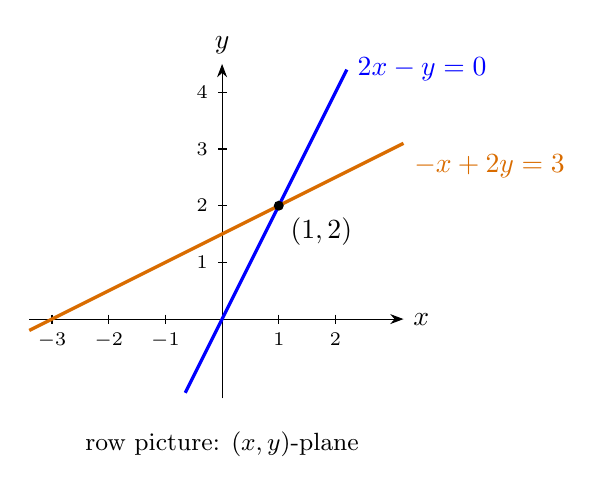
\begin{tikzpicture}[scale=0.72,>=Stealth]
  \draw[->] (-3.4,0) -- (3.2,0) node[right] {$x$};
  \draw[->] (0,-1.4) -- (0,4.5) node[above] {$y$};
  \foreach \t in {-3,-2,-1,1,2} \draw (\t,0.08) -- (\t,-0.08) node[below] {\scriptsize $\t$};
  \foreach \t in {1,2,3,4} \draw (0.08,\t) -- (-0.08,\t) node[left] {\scriptsize $\t$};
  \draw[very thick,blue] (-0.65,-1.3) -- (2.2,4.4) node[right] {$2x-y=0$};
  \draw[very thick,orange!85!black] (-3.4,-0.2) -- (3.2,3.1) node[below right] {$-x+2y=3$};
  \fill (1,2) circle (2.5pt) node[below right=1pt] {$(1,2)$};
  \node[font=\small] at (0,-2.2) {row picture: $(x,y)$-plane};
\end{tikzpicture}
\qquad
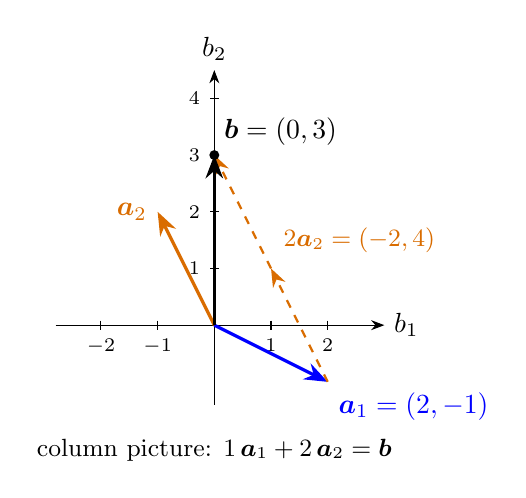
\begin{tikzpicture}[scale=0.72,>=Stealth]
  \draw[->] (-2.8,0) -- (3,0) node[right] {$b_1$};
  \draw[->] (0,-1.4) -- (0,4.5) node[above] {$b_2$};
  \foreach \t in {-2,-1,1,2} \draw (\t,0.08) -- (\t,-0.08) node[below] {\scriptsize $\t$};
  \foreach \t in {1,2,3,4} \draw (0.08,\t) -- (-0.08,\t) node[left] {\scriptsize $\t$};
  \draw[->,very thick,blue] (0,0) -- (2,-1) node[below right] {$\vb{a}_1=(2,-1)$};
  \draw[->,very thick,orange!85!black] (0,0) -- (-1,2) node[left] {$\vb{a}_2$};
  \draw[->,thick,dashed,orange!85!black] (2,-1) -- (1,1);
  \draw[->,thick,dashed,orange!85!black] (1,1) -- (0,3);
  \node[orange!85!black,right,font=\small] at (1.05,1.5) {$2\vb{a}_2=(-2,4)$};
  \draw[->,very thick] (0,0) -- (0,3);
  \fill (0,3) circle (2.5pt) node[above right] {$\vb{b}=(0,3)$};
  \node[font=\small] at (0,-2.2) {column picture: $1\,\vb{a}_1+2\,\vb{a}_2=\vb{b}$};
\end{tikzpicture}
\caption{The system $2x-y=0$, $-x+2y=3$ two ways. Left: each equation is a line and the
solution is the crossing point $(1,2)$. Right: the columns $\vb{a}_1,\vb{a}_2$ are arrows in
the plane of right-hand sides; one $\vb{a}_1$ followed by two copies of $\vb{a}_2$ (dashed,
tip to tail) lands on $\vb{b}=(0,3)$. The weights $1,2$ are the coordinates of the crossing
point.}\label{fig:u01-pictures}
\end{figure}

The two panels live in different planes. In the row picture the axes are the unknowns
$x$ and $y$, and the answer is a point. In the column picture the axes are the components
$b_1,b_2$ of the right-hand side (the first and second equations), and the answer is a pair
of weights.

What do \emph{all} combinations $x\vb{a}_1+y\vb{a}_2$ give? Multiples of $\vb{a}_1$ fill a
line through the origin, multiples of $\vb{a}_2$ fill another line, and because the two
lines point in different directions, adding a point of one to a point of the other reaches
every point of the plane. So for this $A$ the system can be solved for \emph{every}
right-hand side $\vb{b}$ (Exercise~\ref{ex:u01-every-b} finds the weights explicitly).

The column picture of the $3\times3$ system \eqref{eq:u01-three} is
\[
  x\begin{bmatrix} 2\\ -1\\ 0\end{bmatrix}
  + y\begin{bmatrix} -1\\ 2\\ -3\end{bmatrix}
  + z\begin{bmatrix} 0\\ -1\\ 4\end{bmatrix}
  = \begin{bmatrix} 0\\ -1\\ 4\end{bmatrix}.
\]
This right-hand side was chosen to equal the third column, so the combination is visible at
once: $x=0$, $y=0$, $z=1$. That is the point where the three planes of the row picture meet,
found without drawing a single plane. If we change the right-hand side to
$\vb{b}=(1,1,-3)$, which is column~1 plus column~2, the solution becomes $(x,y,z)=(1,1,0)$.
In the row picture all three planes moved; in the column picture the three columns stayed
put and only the target changed. Usually the combination is not visible by eye, and the
systematic method of finding it, elimination, is the subject of Section~\ref{sec:u03}.

\subsection{Multiplying a matrix by a vector}\label{subsec:u01-product}

The column picture tells us what $A\vb{x}$ should mean.

\begin{definition}[Matrix times vector]\label{def:u01-Ax}
Let $A$ be an $m\times n$ matrix with columns $\vb{a}_1,\dots,\vb{a}_n$ (each in $\R^m$),
and let $\vb{x}=(x_1,\dots,x_n)\in\R^n$. The product $A\vb{x}$ is the combination of the
columns with weights from $\vb{x}$:
\[
  A\vb{x} = x_1\vb{a}_1 + x_2\vb{a}_2 + \cdots + x_n\vb{a}_n \in \R^m .
\]
\end{definition}

The product is defined only when the number of columns of $A$ equals the number of
components of $\vb{x}$. The familiar ``row times vector'' rule is the same computation
organised differently.

\begin{proposition}[Row form of $A\vb{x}$]\label{prop:u01-rows}
For $A$ and $\vb{x}$ as in Definition~\ref{def:u01-Ax}, component $i$ of $A\vb{x}$ is the
dot product of row $i$ of $A$ with $\vb{x}$:
\[
  (A\vb{x})_i = a_{i1}x_1 + a_{i2}x_2 + \cdots + a_{in}x_n = \sum_{j=1}^{n} a_{ij}x_j .
\]
\end{proposition}

\begin{proof}
Component $i$ of the vector $x_j\vb{a}_j$ is $x_j$ times component $i$ of $\vb{a}_j$, which
is $a_{ij}x_j$. Components of a sum are sums of components, so component $i$ of
$x_1\vb{a}_1+\cdots+x_n\vb{a}_n$ is $a_{i1}x_1+\cdots+a_{in}x_n$, and this is row $i$ of $A$
dotted with $\vb{x}$.
\end{proof}

So the row picture corresponds to computing $A\vb{x}$ by rows (each equation is one dot
product), and the column picture corresponds to computing $A\vb{x}$ by columns. With
Definition~\ref{def:u01-Ax}, the shorthand $A\vb{x}=\vb{b}$ for a linear system is now a true
equation between vectors.

\begin{example}[Both ways]\label{ex:u01-both-ways}
Compute $\begin{bmatrix} 2 & 5\\ 1 & 3\end{bmatrix}\begin{bmatrix} 1\\ 2\end{bmatrix}$.
By columns, take one of the first column and two of the second:
\[
  1\begin{bmatrix} 2\\ 1\end{bmatrix} + 2\begin{bmatrix} 5\\ 3\end{bmatrix}
  = \begin{bmatrix} 2+10\\ 1+6\end{bmatrix} = \begin{bmatrix} 12\\ 7\end{bmatrix}.
\]
By rows, $(2,5)\cdot(1,2) = 2+10 = 12$ and $(1,3)\cdot(1,2)=1+6=7$. The same four
multiplications happen in a different order. In particular, if the right-hand side were
$\vb{b}=(12,7)$, the solution of $A\vb{x}=\vb{b}$ would be $\vb{x}=(1,2)$.
\end{example}

\subsection{Can every right-hand side be reached?}

For a given square matrix $A$, can we solve $A\vb{x}=\vb{b}$ for \emph{every} $\vb{b}$?
In the language of the column picture the question becomes: do the linear combinations of
the columns fill the whole space $\R^n$? For the $2\times2$ example the answer was yes,
and for the $3\times3$ matrix of \eqref{eq:u01-three} it is also yes. Such matrices are called
\emph{nonsingular} or \emph{invertible}; Section~\ref{sec:u04} defines the inverse matrix
that undoes $A$. When the answer is no, $A$ is \emph{singular}.

Here is how the answer can fail in three dimensions. If the three columns happen to lie in
one plane through the origin, every combination of them lies in that plane too, and no
right-hand side off the plane can be produced.

\begin{proposition}[A dependent column adds nothing]\label{prop:u01-dependent}
Let $A$ have columns $\vb{a}_1,\vb{a}_2,\vb{a}_3$ in $\R^3$ and suppose
$\vb{a}_3 = c_1\vb{a}_1 + c_2\vb{a}_2$. Then every vector $A\vb{x}$ is a combination of
$\vb{a}_1$ and $\vb{a}_2$ alone.
\end{proposition}

\begin{proof}
For any $\vb{x}=(x_1,x_2,x_3)$,
\[
  A\vb{x} = x_1\vb{a}_1 + x_2\vb{a}_2 + x_3(c_1\vb{a}_1+c_2\vb{a}_2)
  = (x_1+c_1x_3)\,\vb{a}_1 + (x_2+c_2x_3)\,\vb{a}_2 . \qedhere
\]
\end{proof}

The combinations of two vectors in $\R^3$ fill at most a plane through the origin, so a
matrix with a dependent column is singular: some $\vb{b}$ are out of reach. (That two
vectors cannot fill $\R^3$ is intuitively clear; the precise statement, that a space of
dimension $3$ needs three independent vectors, is proved in Section~\ref{sec:u10}.)

\begin{example}[Three columns in a plane]\label{ex:u01-plane}
Let $\vb{w}_1=(1,2,3)$, $\vb{w}_2=(4,5,6)$, $\vb{w}_3=(7,8,9)$. Find a combination
$x_1\vb{w}_1+x_2\vb{w}_2+x_3\vb{w}_3$ that gives the zero vector, and a vector $\vb{b}$ that
is not a combination of them.

The requirement is three equations:
\[
  x_1+4x_2+7x_3=0,\qquad 2x_1+5x_2+8x_3=0,\qquad 3x_1+6x_2+9x_3=0 .
\]
Subtract twice the first equation from the second: $-3x_2-6x_3=0$. Subtract three times
the first from the third: $-6x_2-12x_3=0$, which is twice the previous equation and so
tells us nothing new. Choose $x_3=1$; then $x_2=-2$ and $x_1=-4x_2-7x_3=8-7=1$. Hence
\[
  \vb{w}_1 - 2\vb{w}_2 + \vb{w}_3 = (1-8+7,\; 2-10+8,\; 3-12+9) = (0,0,0).
\]
The vectors are \emph{dependent}: $\vb{w}_2=\tfrac12(\vb{w}_1+\vb{w}_3)$ lies in the plane
of $\vb{w}_1$ and $\vb{w}_3$, so all three lie in one plane through the origin. Which plane?
Each $\vb{w}_j=(w_1,w_2,w_3)$ satisfies $w_1-2w_2+w_3=0$ ($1-4+3=0$, $4-10+6=0$,
$7-16+9=0$), and that equation is preserved by adding vectors and multiplying by scalars. So
every combination $\vb{b}$ satisfies $b_1-2b_2+b_3=0$. The vector $\vb{b}=(1,0,0)$ gives
$1\neq0$, so $W\vb{x}=(1,0,0)$ has no solution for the matrix $W$ with columns
$\vb{w}_1,\vb{w}_2,\vb{w}_3$, and $W$ is not invertible.
\end{example}

The same thinking works in any dimension, even where nothing can be drawn. Nine equations
in nine unknowns give nine columns, each a vector in $\R^9$. A matrix with random entries
almost certainly has columns whose combinations fill all of $\R^9$. But if, say, the ninth
column equals the eighth, it contributes nothing new, and the combinations fill only an
eight-dimensional ``plane'' through the origin inside $\R^9$. Learning to think about such
flat pieces of high-dimensional space is the heart of the course.

\begin{trap}
Do not mix up the two pictures. In the row picture the point $(1,2)$ is a \emph{location}
in the plane of unknowns; in the column picture the same numbers are \emph{weights}, and the
arrows live in the plane of right-hand sides, where the target is $\vb{b}=(0,3)$, not
$(1,2)$. Likewise, $A\vb{x}$ is not only ``rows dotted with $\vb{x}$'': it is a combination
of the columns of $A$, and that is the view that keeps working when no lines or planes can
be drawn.
\end{trap}

\subsection{Exercises}

\begin{exercise}\label{ex:u01-multiply}
Compute $\begin{bmatrix} 1 & 2 & 0\\ 2 & 0 & 3\\ 4 & 1 & 1\end{bmatrix}
\begin{bmatrix} 3\\ -2\\ 1\end{bmatrix}$ by rows, and again as a combination of columns.
\end{exercise}
\begin{solution}
By rows: $1\cdot3+2\cdot(-2)+0\cdot1=-1$, then $2\cdot3+0\cdot(-2)+3\cdot1=9$, then
$4\cdot3+1\cdot(-2)+1\cdot1=11$. By columns:
\[
  3\begin{bmatrix} 1\\ 2\\ 4\end{bmatrix} - 2\begin{bmatrix} 2\\ 0\\ 1\end{bmatrix}
  + 1\begin{bmatrix} 0\\ 3\\ 1\end{bmatrix}
  = \begin{bmatrix} 3-4+0\\ 6-0+3\\ 12-2+1\end{bmatrix}
  = \begin{bmatrix} -1\\ 9\\ 11\end{bmatrix}. \qedhere
\]
\end{solution}

\begin{exercise}\label{ex:u01-shapes}
True or false: a $3\times2$ matrix $A$ times a $2\times3$ matrix $B$ is a $3\times3$ matrix
$AB$. State the general rule for the shapes. (Think of $AB$ as $A$ multiplying each column
of $B$; Section~\ref{sec:u04} develops this.)
\end{exercise}
\begin{solution}
True. Each column of $B$ has $2$ components, which matches the $2$ columns of $A$, so $A$
can multiply it and produces a vector with $3$ components. $B$ has $3$ columns, so $AB$ has
$3$ columns of length $3$. In general an $m\times n$ matrix times an $n\times p$ matrix is
$m\times p$: the inner dimensions must agree and the outer ones give the shape.
\end{solution}

\begin{exercise}\label{ex:u01-recitation}
Solve $2x+y=3$, $x-2y=-1$. Sketch the row picture (find two points on each line) and the
column picture, and write the system in matrix form.
\end{exercise}
\begin{solution}
From the second equation $x=2y-1$; substituting, $2(2y-1)+y=3$, so $5y=5$, $y=1$ and $x=1$.
Row picture: $2x+y=3$ passes through $(0,3)$ and $(1,1)$; $x-2y=-1$ passes through
$(0,\tfrac12)$ and $(1,1)$; the lines cross at $(1,1)$. Column picture: the columns are
$\vb{v}_1=(2,1)$ and $\vb{v}_2=(1,-2)$, and one of each gives the diagonal of the
parallelogram they span, $(2+1,\,1-2)=(3,-1)=\vb{b}$. Matrix form:
$\begin{bmatrix} 2 & 1\\ 1 & -2\end{bmatrix}\begin{bmatrix} x\\ y\end{bmatrix}
=\begin{bmatrix} 3\\ -1\end{bmatrix}$.
\end{solution}

\begin{exercise}\label{ex:u01-every-b}
With the columns $\vb{a}_1=(2,-1)$ and $\vb{a}_2=(-1,2)$ of Example~\ref{ex:u01-two-pictures},
which combination reaches $\vb{b}=(1,1)$? Then find the weights $x,y$ with
$x\vb{a}_1+y\vb{a}_2=(b_1,b_2)$ for an arbitrary right-hand side, confirming that every $\vb{b}$
is reachable.
\end{exercise}
\begin{solution}
$\vb{a}_1+\vb{a}_2=(2-1,\,-1+2)=(1,1)$, so $x=y=1$. In general we need $2x-y=b_1$ and
$-x+2y=b_2$. Adding twice the first equation to the second gives $3x=2b_1+b_2$; adding the
first to twice the second gives $3y=b_1+2b_2$. So
\[
  x=\frac{2b_1+b_2}{3},\qquad y=\frac{b_1+2b_2}{3}.
\]
Check: $2x-y=\frac{4b_1+2b_2-b_1-2b_2}{3}=b_1$ and $-x+2y=\frac{-2b_1-b_2+2b_1+4b_2}{3}=b_2$.
Weights exist for every $\vb{b}$, so the columns fill the plane. For $\vb{b}=(1,1)$ the
formula gives $x=y=1$ again.
\end{solution}

\begin{exercise}\label{ex:u01-param}
The matrix $A$ has columns $(1,0,1)$, $(0,1,1)$ and $(1,1,c)$. For $c=2$, show that the
columns lie in a plane, find an equation of that plane, and give a right-hand side $\vb{b}$
for which $A\vb{x}=\vb{b}$ has no solution. For $c=3$, solve $A\vb{x}=(0,0,1)$.
\end{exercise}
\begin{solution}
For $c=2$ the third column is $(1,0,1)+(0,1,1)$, so by
Proposition~\ref{prop:u01-dependent} every $A\vb{x}$ is a combination
$s(1,0,1)+t(0,1,1)=(s,\,t,\,s+t)$. These vectors satisfy $b_3=b_1+b_2$, the equation of
the plane. The vector $\vb{b}=(0,0,1)$ has $b_3=1\neq0=b_1+b_2$, so it is unreachable.

For $c=3$ we need $x_1+x_3=0$, $x_2+x_3=0$ and $x_1+x_2+3x_3=1$. The first two give
$x_1=x_2=-x_3$, and the third becomes $-x_3-x_3+3x_3=x_3=1$. So $\vb{x}=(-1,-1,1)$, and
indeed $-(1,0,1)-(0,1,1)+(1,1,3)=(0,0,1)$. The column $(1,1,3)$ is off the plane
$b_3=b_1+b_2$, which is why the target off that plane can now be reached.
\end{solution}

% unit: u02
% sources: sources/068-an-overview-of-key-ideas.txt, sources/120-an-overview-of-linear-algebra.txt, sources/121-mit18-06scf11-ses1-13sum-pdf-download-file.txt, sources/122-an-overview-of-key-ideas.txt, short_plan.json (s01)
\section{An overview of key ideas}\label{sec:u02}

Before the course settles into elimination, it is worth seeing the whole road at once.
Linear algebra moves from \emph{vectors} to \emph{matrices} to \emph{subspaces}: what you do
with vectors is take combinations; a matrix packages those combinations as a single
operation $\vb{x}\mapsto A\vb{x}$; and the set of all combinations is a subspace. This
section, adapted from Strang's opening review in 18.085, follows two $3\times3$ matrices that
differ in a single column. One is invertible and its inverse can be written down by hand; the
other has dependent columns, solves $C\vb{x}=\vb{b}$ only for special $\vb{b}$, and shows
what a subspace is. Almost every idea of Part~I appears here in preview, and later sections
make each one precise.

\subsection{Vectors: take their combinations}

Work in $\R^3$, the space of vectors with three real components, with
\[
  \vb{u}=\begin{bmatrix} 1\\ -1\\ 0\end{bmatrix},\qquad
  \vb{v}=\begin{bmatrix} 0\\ 1\\ -1\end{bmatrix},\qquad
  \vb{w}=\begin{bmatrix} 0\\ 0\\ 1\end{bmatrix}.
\]
The only operations we need are multiplying a vector by a scalar and adding vectors, which
together produce linear combinations $x_1\vb{u}+x_2\vb{v}+x_3\vb{w}$
(Definition~\ref{def:u01-combination}). All multiples $c\,\vb{u}$ fill a line through the
origin. All multiples of $\vb{v}$ fill a second line. Because $\vb{v}$ is not a multiple of
$\vb{u}$, the combinations $x_1\vb{u}+x_2\vb{v}$ fill something bigger than either line: a
plane through the origin. Whether adding $\vb{w}$ fills all of $\R^3$ is the question the
rest of the section answers.

\subsection{Matrices: the difference matrix and its inverse}

Put the three vectors into the columns of a matrix. Then the combination with weights
$x_1,x_2,x_3$ is exactly the matrix-vector product of Definition~\ref{def:u01-Ax}:
\begin{equation}\label{eq:u02-A}
  A\vb{x}=\begin{bmatrix} 1 & 0 & 0\\ -1 & 1 & 0\\ 0 & -1 & 1\end{bmatrix}
  \begin{bmatrix} x_1\\ x_2\\ x_3\end{bmatrix}
  = x_1\vb{u}+x_2\vb{v}+x_3\vb{w}
  = \begin{bmatrix} x_1\\ x_2-x_1\\ x_3-x_2\end{bmatrix}.
\end{equation}
The calculation is the same as before but the point of view has changed. Before, numbers
$x_j$ multiplied vectors; now the matrix $A$ acts on the vector $\vb{x}$ and produces an
output. This $A$ is a \emph{difference matrix}: each output component is a difference of
consecutive inputs (with $x_0=0$).

\begin{example}[Differences of squares]\label{ex:u02-squares}
Feed in the squares $\vb{x}=(1,4,9)$:
\[
  A\begin{bmatrix} 1\\ 4\\ 9\end{bmatrix}
  =\begin{bmatrix} 1\\ 4-1\\ 9-4\end{bmatrix}=\begin{bmatrix} 1\\ 3\\ 5\end{bmatrix}.
\]
Differences of consecutive squares are the odd numbers, since $(k+1)^2-k^2=2k+1$.
\end{example}

The deeper question runs backwards: given the output $\vb{b}$, find the input $\vb{x}$ with
$A\vb{x}=\vb{b}$. The three equations are
\[
  x_1=b_1,\qquad x_2-x_1=b_2,\qquad x_3-x_2=b_3 .
\]
Because $A$ is lower triangular they can be solved from the top down: $x_1=b_1$, then
$x_2=b_1+b_2$, then $x_3=b_1+b_2+b_3$. Read the answer as a matrix times $\vb{b}$: the
coefficients of $b_1$ form the first column, and so on.
\begin{equation}\label{eq:u02-S}
  \vb{x}=\begin{bmatrix} b_1\\ b_1+b_2\\ b_1+b_2+b_3\end{bmatrix}
  =\begin{bmatrix} 1 & 0 & 0\\ 1 & 1 & 0\\ 1 & 1 & 1\end{bmatrix}
  \begin{bmatrix} b_1\\ b_2\\ b_3\end{bmatrix} = S\vb{b}.
\end{equation}
The matrix $S$ takes running sums. It undoes $A$, and $A$ undoes $S$:

\begin{proposition}[The sum matrix inverts the difference matrix]\label{prop:u02-sum}
For every $\vb{x}\in\R^3$, $S(A\vb{x})=\vb{x}$, and for every $\vb{b}\in\R^3$,
$A(S\vb{b})=\vb{b}$. Consequently $A\vb{x}=\vb{b}$ has exactly one solution for every
$\vb{b}$, namely $\vb{x}=S\vb{b}$, and $A\vb{x}=\vb{0}$ only for $\vb{x}=\vb{0}$.
\end{proposition}

\begin{proof}
Running sums of differences telescope:
\[
  S(A\vb{x}) = S\begin{bmatrix} x_1\\ x_2-x_1\\ x_3-x_2\end{bmatrix}
  = \begin{bmatrix} x_1\\ x_1+(x_2-x_1)\\ x_1+(x_2-x_1)+(x_3-x_2)\end{bmatrix}
  = \begin{bmatrix} x_1\\ x_2\\ x_3\end{bmatrix}.
\]
Differences of running sums return the original entries:
$A(S\vb{b}) = \bigl(b_1,\ (b_1+b_2)-b_1,\ (b_1+b_2+b_3)-(b_1+b_2)\bigr)=(b_1,b_2,b_3)$.
The second identity shows that $\vb{x}=S\vb{b}$ solves $A\vb{x}=\vb{b}$. If $\vb{x}$ is any
solution, then $\vb{x}=S(A\vb{x})=S\vb{b}$ by the first identity, so the solution is unique.
With $\vb{b}=\vb{0}$ this unique solution is $S\vb{0}=\vb{0}$.
\end{proof}

A matrix that undoes $A$ in this way is called the \emph{inverse} of $A$ and written
$A^{-1}$; here $A^{-1}=S$. Section~\ref{sec:u04} defines inverses in general and shows how to
compute them. Think of $A$ as a transform taking $\vb{x}$ to $\vb{b}$ and of $S$ as the
inverse transform taking $\vb{b}$ back to $\vb{x}$. For example $S(1,3,5)=(1,1+3,1+3+5)=(1,4,9)$
recovers the squares. Calculus has the same structure: differences are the discrete version of
the derivative, running sums the discrete version of the integral, and
Proposition~\ref{prop:u02-sum} is a small fundamental theorem of calculus.

\subsection{The cyclic difference matrix}

Keep $\vb{u}$ and $\vb{v}$ but replace $\vb{w}$ by $\vb{w}^{*}=(-1,0,1)$. The new matrix
\begin{equation}\label{eq:u02-C}
  C\vb{x}=\begin{bmatrix} 1 & 0 & -1\\ -1 & 1 & 0\\ 0 & -1 & 1\end{bmatrix}
  \begin{bmatrix} x_1\\ x_2\\ x_3\end{bmatrix}
  =\begin{bmatrix} x_1-x_3\\ x_2-x_1\\ x_3-x_2\end{bmatrix}
\end{equation}
still takes differences, but now cyclically: the first row compares $x_1$ with $x_3$, as if
the three entries sat on a circle. Only one column changed, yet $C$ behaves completely
differently from $A$.

\emph{Zero output from a nonzero input.} If $x_1=x_2=x_3=c$, every difference is zero, so
$C(c,c,c)=\vb{0}$. A whole line of inputs, all multiples of $(1,1,1)$, is sent to zero.

\begin{proposition}[No inverse when a nonzero vector goes to zero]\label{prop:u02-noinverse}
If $C\vb{x}=\vb{0}$ for some $\vb{x}\neq\vb{0}$, then there is no matrix $T$ with
$T(C\vb{y})=\vb{y}$ for all $\vb{y}$; that is, $C$ has no inverse.
\end{proposition}

\begin{proof}
Such a $T$ would give $\vb{x}=T(C\vb{x})=T\vb{0}=\vb{0}$, since any matrix times the zero
vector is the zero vector. This contradicts $\vb{x}\neq\vb{0}$. Once $C$ has crushed
$\vb{x}$ to zero, nothing can bring it back.
\end{proof}

\emph{Solvable only for special right-hand sides.} Write out $C\vb{x}=\vb{b}$ and add the
three equations. The left sides cancel, $(x_1-x_3)+(x_2-x_1)+(x_3-x_2)=0$, so the right
sides must satisfy $0=b_1+b_2+b_3$. This condition is not only necessary but sufficient.

\begin{proposition}[When the cyclic system is solvable]\label{prop:u02-solvable}
$C\vb{x}=\vb{b}$ has a solution if and only if $b_1+b_2+b_3=0$. In that case the solutions
are exactly
\[
  \vb{x} = \begin{bmatrix} 0\\ b_2\\ b_2+b_3\end{bmatrix} + c\begin{bmatrix} 1\\ 1\\ 1\end{bmatrix},
  \qquad c\in\R .
\]
\end{proposition}

\begin{proof}
Necessity was shown above by adding the equations. Conversely, suppose $b_1+b_2+b_3=0$ and
let $\vb{x}_p=(0,\,b_2,\,b_2+b_3)$. Then
\[
  C\vb{x}_p = \begin{bmatrix} 0-(b_2+b_3)\\ b_2-0\\ (b_2+b_3)-b_2\end{bmatrix}
  = \begin{bmatrix} b_1\\ b_2\\ b_3\end{bmatrix},
\]
using $-(b_2+b_3)=b_1$. Adding $c(1,1,1)$ does not change $C\vb{x}$, because
$C(c,c,c)=\vb{0}$. Finally, if $\vb{x}$ is any solution, then $\vb{y}=\vb{x}-\vb{x}_p$ satisfies
$C\vb{y}=\vb{b}-\vb{b}=\vb{0}$, so $y_2-y_1=0$ and $y_3-y_2=0$; hence $\vb{y}=c(1,1,1)$ for
some $c$, and every solution has the stated form.
\end{proof}

In a physical model where $x_1,x_2,x_3$ are positions of masses joined in a ring by springs
and $\vb{b}$ holds the applied forces, the condition $b_1+b_2+b_3=0$ says the forces must
balance; the free constant $c$ says the whole ring can be shifted without changing any
spring.

\begin{example}[Solving and failing with $C$]\label{ex:u02-cyclic}
Take $\vb{b}=(1,2,-3)$. Its components sum to $0$, so the system is solvable, and
Proposition~\ref{prop:u02-solvable} gives $\vb{x}_p=(0,\,2,\,2-3)=(0,2,-1)$. Check:
$C\vb{x}_p=(0-(-1),\ 2-0,\ -1-2)=(1,2,-3)$. All solutions are $(0,2,-1)+c(1,1,1)$, for
instance $(1,3,0)$ with $c=1$. For $\vb{b}=(1,1,1)$ the components sum to $3\neq0$, and
$C\vb{x}=\vb{b}$ has no solution at all.
\end{example}

\subsection{Subspaces: what all the combinations fill}

Which vectors $\vb{b}$ are combinations of the columns $\vb{u},\vb{v},\vb{w}^{*}$ of $C$?
Each column has components adding to zero, and that property survives addition and
scalar multiplication, so every combination $C\vb{x}$ lies on the plane
$b_1+b_2+b_3=0$. Proposition~\ref{prop:u02-solvable} says that every vector on that plane is
reached. So \emph{all vectors $C\vb{x}$} form exactly the plane $b_1+b_2+b_3=0$. In fact
$\vb{w}^{*}=-(\vb{u}+\vb{v})$ lies in the plane of $\vb{u}$ and $\vb{v}$ and adds nothing
new (Proposition~\ref{prop:u01-dependent}). For $A$, Proposition~\ref{prop:u02-sum} says
every $\vb{b}$ in $\R^3$ is reached, so the combinations of $\vb{u},\vb{v},\vb{w}$ fill all of
$\R^3$. Figure~\ref{fig:u02-plane} shows the difference.

\begin{figure}[ht]
\centering
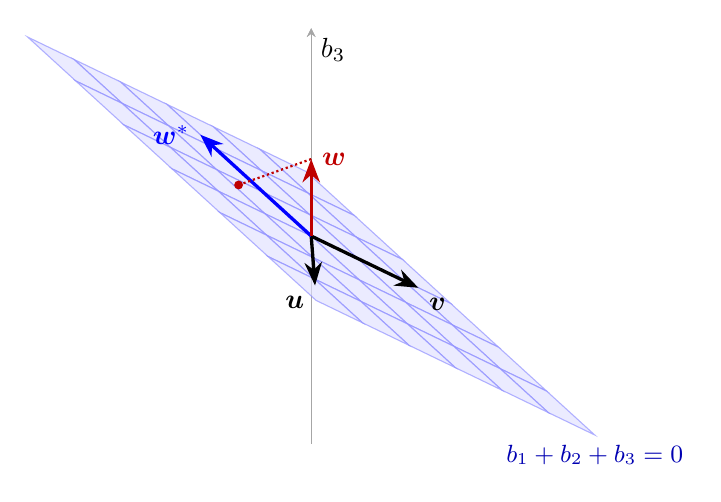
\begin{tikzpicture}[>=Stealth]
\begin{axis}[view={44}{16}, width=11cm, height=9cm, axis x line=none, axis y line=none, axis z line=center, axis line style={gray!70},
  ticks=none, zlabel={$b_3$},
  xmin=-1.7, xmax=1.7, ymin=-1.7, ymax=1.7, zmin=-2.7, zmax=2.7, clip=false]
  \addplot3[surf, shader=faceted, colormap={single}{color=(blue!12) color=(blue!12)},
    faceted color=blue!45, opacity=0.65, samples=7, domain=-1.3:1.3, y domain=-1.3:1.3] {-x-y};
  \draw[->,very thick] (0,0,0) -- (1,-1,0) node[below left] {$\vb{u}$};
  \draw[->,very thick] (0,0,0) -- (0,1,-1) node[below right] {$\vb{v}$};
  \draw[->,very thick,blue] (0,0,0) -- (-1,0,1) node[left] {$\vb{w}^{*}$};
  \draw[->,very thick,red!75!black] (0,0,0) -- (0,0,1) node[right] {$\vb{w}$};
  \draw[thick,densely dotted,red!75!black] (0,0,1) -- (-0.333,-0.333,0.667);
  \fill[red!75!black] (-0.333,-0.333,0.667) circle (1.6pt);
  \node[blue!70!black,font=\small] at (1.3,1.3,-2.6) [below] {$b_1+b_2+b_3=0$};
\end{axis}
\end{tikzpicture}
\caption{The columns $\vb{u}=(1,-1,0)$, $\vb{v}=(0,1,-1)$ and $\vb{w}^{*}=(-1,0,1)$ of the
cyclic matrix $C$ all lie in the plane $b_1+b_2+b_3=0$ (shaded), so every $C\vb{x}$ stays in
that plane. The third column $\vb{w}=(0,0,1)$ of the difference matrix $A$ points out of the
plane (the dotted segment drops from its tip to the nearest point of the plane), so the
combinations of $\vb{u},\vb{v},\vb{w}$ fill all of $\R^3$.}\label{fig:u02-plane}
\end{figure}

Here are the words for what we have seen; Sections~\ref{sec:u06}, \ref{sec:u07} and
\ref{sec:u10} develop them in full.

\begin{definition}[Independent and dependent vectors]\label{def:u02-independent}
Vectors $\vb{v}_1,\dots,\vb{v}_n$ are \emph{dependent} if some combination
$c_1\vb{v}_1+\cdots+c_n\vb{v}_n$ with weights not all zero equals the zero vector. Otherwise
they are \emph{independent}: the only combination giving $\vb{0}$ is the one with all
weights zero.
\end{definition}

In matrix language, the columns of a matrix are independent exactly when $A\vb{x}=\vb{0}$
forces $\vb{x}=\vb{0}$. So $\vb{u},\vb{v},\vb{w}$ are independent
(Proposition~\ref{prop:u02-sum}), while $\vb{u}+\vb{v}+\vb{w}^{*}=C(1,1,1)=\vb{0}$ shows that
$\vb{u},\vb{v},\vb{w}^{*}$ are dependent.

\begin{definition}[Vector space, subspace, basis]\label{def:u02-subspace}
A \emph{vector space} is a collection of vectors closed under linear combinations: any
combination of vectors in the collection is again in it. A \emph{subspace} is a vector space
contained in a larger one. A \emph{basis} of $\R^n$ is a set of $n$ independent vectors in
$\R^n$.
\end{definition}

The plane $b_1+b_2+b_3=0$ is a subspace of $\R^3$: it is the set of all combinations of
$\vb{u}$ and $\vb{v}$, and a combination of combinations is a combination. A filled triangle
with corners $\vb{0},\vb{u},\vb{v}$ is \emph{not} a subspace, because $2\vb{u}$ leaves it.
Taking all combinations of some vectors is the standard way to build a subspace, and it
always produces a subspace. The subspaces of $\R^3$ are: the origin alone, the lines
through the origin, the planes through the origin, and $\R^3$ itself, of dimensions
$0,1,2,3$. The zero vector belongs to every one of them, since $0\cdot\vb{v}=\vb{0}$.

For $n$ vectors in $\R^n$ there are three equivalent ways to say ``basis'', which this
section has seen side by side for $\vb{u},\vb{v},\vb{w}$: (i) the vectors are independent;
(ii) their combinations fill $\R^n$; (iii) the $n\times n$ matrix with those columns is
invertible. The vectors $\vb{u},\vb{v},\vb{w}^{*}$ fail all three. The proof that the three
statements always agree comes in Section~\ref{sec:u10}.

\begin{example}[A basis of the plane from Section~\ref{sec:u01}]\label{ex:u02-basis2}
The columns $\vb{a}_1=(2,-1)$ and $\vb{a}_2=(-1,2)$ of the first example of the course form a
basis of $\R^2$. They are independent: if $c_1\vb{a}_1+c_2\vb{a}_2=\vb{0}$ then
$2c_1-c_2=0$ and $-c_1+2c_2=0$; the first gives $c_2=2c_1$, and the second becomes
$-c_1+4c_1=3c_1=0$, so $c_1=c_2=0$. Their combinations fill $\R^2$: we found
$1\,\vb{a}_1+2\,\vb{a}_2=(0,3)$, and $\vb{a}_1+\vb{a}_2=(1,1)$, and
Exercise~\ref{ex:u01-every-b} gives the weights for every $\vb{b}$. And the matrix
$\begin{bmatrix} 2 & -1\\ -1 & 2\end{bmatrix}$ is invertible, since each $\vb{b}$ has exactly
one pair of weights.
\end{example}

\begin{trap}
Dependence is not the same as ``two columns are parallel''. No column of $C$ is a multiple of
another, yet the three columns are dependent because $\vb{u}+\vb{v}+\vb{w}^{*}=\vb{0}$. To
test three vectors you must look for a combination of all of them, not compare them in pairs.
\end{trap}

\subsection{Looking ahead: rectangular matrices}

The habit to build is to look at a matrix and ask what it \emph{does}. $A$ takes differences
and can be undone; $C$ takes cyclic differences, crushes the constant vectors and reaches
only a plane. Matrices need not be square: a $7\times3$ matrix sends $\R^3$ into $\R^7$, can
reach at most a three-dimensional part of $\R^7$, and has no inverse. A matrix that keeps
appearing with rectangular $A$ is $A\T A$: it is square ($3\times3$ here) and symmetric, and
it will be the key to least squares in Part~II (Section~\ref{sec:u17}).

\subsection{Exercises}

\begin{exercise}\label{ex:u02-quiz}
A matrix $A$ has the property that \emph{all} solutions of $A\vb{x}=(1,4,1,1)$ are
\[
  \vb{x}=\begin{bmatrix} 0\\ 1\\ 1\end{bmatrix} + c\begin{bmatrix} 0\\ 2\\ 1\end{bmatrix},
  \qquad c\in\R .
\]
Say everything you can about the columns $\vb{c}_1,\vb{c}_2,\vb{c}_3$ of $A$.
\end{exercise}
\begin{solution}
Since $\vb{x}$ has three components, $A$ has three columns, and since $\vb{b}=(1,4,1,1)$ has
four, each column lies in $\R^4$. Taking $c=0$ gives $A(0,1,1)=\vb{b}$, that is,
$\vb{c}_2+\vb{c}_3=\vb{b}$. Taking $c=1$ gives $A(0,3,2)=\vb{b}$; subtracting,
$A(0,2,1)=\vb{0}$, that is, $2\vb{c}_2+\vb{c}_3=\vb{0}$. Subtract the first relation from the
second: $\vb{c}_2=-\vb{b}$, and then $\vb{c}_3=\vb{b}-\vb{c}_2=2\vb{b}$. So
$\vb{c}_2=(-1,-4,-1,-1)$ and $\vb{c}_3=(2,8,2,2)$.

About $\vb{c}_1$: it cannot be a multiple of $\vb{b}$. If $\vb{c}_1=k\vb{b}$, then
$A(1,k,0)=k\vb{b}-k\vb{b}=\vb{0}$, and $(0,1,1)+(1,k,0)$ would be another solution of
$A\vb{x}=\vb{b}$ whose first component is $1$, which is not of the given form. Conversely,
if $\vb{c}_1$ is not a multiple of $\vb{b}$, then $A\vb{x}=x_1\vb{c}_1+(2x_3-x_2)\vb{b}=\vb{0}$
forces $x_1=0$ and $x_2=2x_3$ (two non-parallel vectors combine to zero only with zero
weights), so the solutions of $A\vb{x}=\vb{0}$ are exactly the multiples of $(0,2,1)$, as
required. Hence: $\vb{c}_1$ is any vector of $\R^4$ that is not a multiple of $\vb{b}$
(in particular not $\vb{0}$), and nothing more can be said.
\end{solution}

\begin{exercise}\label{ex:u02-four}
Let $A_4$ be the $4\times4$ difference matrix, $A_4\vb{x}=(x_1,\,x_2-x_1,\,x_3-x_2,\,x_4-x_3)$.
Write $A_4$ and its inverse $S_4$, and use $S_4$ to solve $A_4\vb{x}=(1,3,5,7)$.
\end{exercise}
\begin{solution}
Solving from the top, $x_1=b_1$, $x_2=b_1+b_2$, $x_3=b_1+b_2+b_3$,
$x_4=b_1+b_2+b_3+b_4$, so
\[
  A_4=\begin{bmatrix} 1&0&0&0\\ -1&1&0&0\\ 0&-1&1&0\\ 0&0&-1&1\end{bmatrix},\qquad
  S_4=A_4^{-1}=\begin{bmatrix} 1&0&0&0\\ 1&1&0&0\\ 1&1&1&0\\ 1&1&1&1\end{bmatrix}.
\]
Then $\vb{x}=S_4(1,3,5,7)=(1,\,4,\,9,\,16)$: running sums of odd numbers are the squares.
Check: $A_4(1,4,9,16)=(1,3,5,7)$.
\end{solution}

\begin{exercise}\label{ex:u02-cyclic}
For the cyclic matrix $C$ of \eqref{eq:u02-C}, decide which of $\vb{b}=(1,0,-1)$,
$(2,-3,1)$ and $(1,1,0)$ lie in the plane of all $C\vb{x}$, and solve $C\vb{x}=\vb{b}$ when it
is possible.
\end{exercise}
\begin{solution}
Use Proposition~\ref{prop:u02-solvable}. For $(1,0,-1)$ the sum is $0$; the particular
solution is $(0,\,b_2,\,b_2+b_3)=(0,0,-1)$, and indeed $C(0,0,-1)=(0+1,\,0-0,\,-1-0)=(1,0,-1)$.
All solutions: $(0,0,-1)+c(1,1,1)$. For $(2,-3,1)$ the sum is $0$; the particular solution
is $(0,-3,-2)$, and $C(0,-3,-2)=(0+2,\,-3-0,\,-2+3)=(2,-3,1)$. All solutions:
$(0,-3,-2)+c(1,1,1)$. For $(1,1,0)$ the sum is $2\neq0$, so this $\vb{b}$ is off the plane
and there is no solution.
\end{solution}

\begin{exercise}\label{ex:u02-which}
Which of these subsets of $\R^3$ are subspaces? (a) all $\vb{b}$ with $b_1+b_2+b_3=0$;
(b) all $\vb{b}$ with $b_1+b_2+b_3=1$; (c) all multiples of $(1,1,1)$; (d) all $\vb{b}$
with $b_1\ge0$; (e) the zero vector alone.
\end{exercise}
\begin{solution}
(a) Yes: it is the plane of all combinations of $\vb{u}$ and $\vb{v}$, and directly, if two
vectors have component sums $0$, so does $c\vb{b}+d\vb{b}'$. (b) No: the zero vector has sum
$0\neq1$, and every subspace contains $\vb{0}$. (c) Yes: a line through the origin;
$c(1,1,1)+d(1,1,1)=(c+d)(1,1,1)$. It is also the set of $\vb{x}$ with $C\vb{x}=\vb{0}$.
(d) No: $(1,0,0)$ is in the set but $-1\cdot(1,0,0)$ is not; the set is closed under
addition but not under multiplication by negative numbers. (e) Yes: $\vb{0}+\vb{0}=\vb{0}$
and $c\,\vb{0}=\vb{0}$; this is the smallest subspace.
\end{solution}

% unit: u03
% sources: sources/072-elimination-with-matrices.txt, sources/123-lecture-elimination-with-matrices.txt, sources/124-mit18-06scf11-ses1-2sum-pdf-download-file.txt, sources/026-elimination-with-matrices.txt, sources/125-mit18-06scf11-ses1-2prob-pdf-download-file.txt, sources/126-mit18-06scf11-ses1-2sol-pdf-download-file.txt
\section{Elimination with matrices}\label{sec:u03}

Section~\ref{sec:u01} asked which combination of the columns produces $\vb{b}$ but had no
systematic way to find it. \emph{Gaussian elimination} is that way, and it is how essentially
every software package solves $A\vb{x}=\vb{b}$. It subtracts multiples of equations from
other equations until the system is triangular, then solves the triangular system from the
bottom up. This section does elimination by hand, sees how it can fail, and then rewrites
each step as multiplication by a simple matrix. That last move turns a procedure into
algebra, and it is the starting point for the factorization $A=LU$ in Section~\ref{sec:u05}.

\subsection{Pivots and multipliers}

Our example has three equations in three unknowns:
\begin{equation}\label{eq:u03-system}
\begin{aligned}
  x + 2y + z &= 2\\
  3x + 8y + z &= 12\\
  4y + z &= 2
\end{aligned}
\qquad\qquad
A=\begin{bmatrix} 1 & 2 & 1\\ 3 & 8 & 1\\ 0 & 4 & 1\end{bmatrix},\quad
\vb{b}=\begin{bmatrix} 2\\ 12\\ 2\end{bmatrix}.
\end{equation}
Elimination works on the rows of $A$ (the equations), so we write only the numbers.

\begin{definition}[Pivot, multiplier, upper triangular]\label{def:u03-pivot}
Elimination clears the columns of $A$ from left to right. At step $k$ the \emph{pivot} is the
entry in position $(k,k)$ of the current matrix; it must be nonzero. To clear an entry
$a_{ik}$ below the pivot ($i>k$), subtract
\[
  \ell_{ik} = \frac{\text{entry to eliminate}}{\text{pivot}}
\]
times the pivot row $k$ from row $i$. The number $\ell_{ik}$ is the \emph{multiplier}. When
all columns are cleared the result $U$ is \emph{upper triangular}: every entry below the main
diagonal is zero, and the pivots sit on the diagonal.
\end{definition}

\begin{example}[Forward elimination on a $3\times3$ system]\label{ex:u03-forward}
Eliminate below the pivots of the matrix $A$ in \eqref{eq:u03-system}.
\begin{itemize}
  \item \emph{Step $(2,1)$.} The first pivot is $1$. The entry below it is $3$, so
    $\ell_{21}=3/1=3$: subtract $3$ times row $1$ from row $2$, giving
    $(3,8,1)-3(1,2,1)=(0,2,-2)$.
  \item \emph{Step $(3,1)$.} The entry in position $(3,1)$ is already $0$, so
    $\ell_{31}=0$ and nothing changes. (Software still checks this position.)
  \item \emph{Step $(3,2)$.} The second pivot is the $2$ now in position $(2,2)$. The entry
    below it is $4$, so $\ell_{32}=4/2=2$: subtract $2$ times the \emph{new} row $2$ from
    row $3$, giving $(0,4,1)-2(0,2,-2)=(0,0,5)$.
\end{itemize}
The third pivot is $5$, and
\[
  A=\begin{bmatrix} 1 & 2 & 1\\ 3 & 8 & 1\\ 0 & 4 & 1\end{bmatrix}
  \;\longrightarrow\;
  \begin{bmatrix} 1 & 2 & 1\\ 0 & 2 & -2\\ 0 & 4 & 1\end{bmatrix}
  \;\longrightarrow\;
  U=\begin{bmatrix} 1 & 2 & 1\\ 0 & 2 & -2\\ 0 & 0 & 5\end{bmatrix}.
\]
\end{example}
The pivots $1,2,5$ already tell us a great deal about $A$. For instance, their product
$1\cdot2\cdot5=10$ is the determinant of $A$ (Section~\ref{sec:u20}).

The right-hand side must receive the same operations. The convenient bookkeeping is the
\emph{augmented matrix} $[\,A\;\;\vb{b}\,]$, with $\vb{b}$ tacked on as an extra column.
Subtracting $3$ times row~1 changes $12$ into $12-3\cdot2=6$; subtracting $2$ times row~2
changes $2$ into $2-2\cdot6=-10$. Elimination turns $A\vb{x}=\vb{b}$ into $U\vb{x}=\vb{c}$
with $\vb{c}=(2,6,-10)$; Figure~\ref{fig:u03-flow} records the whole computation.

\begin{figure}[ht]
\centering
\small
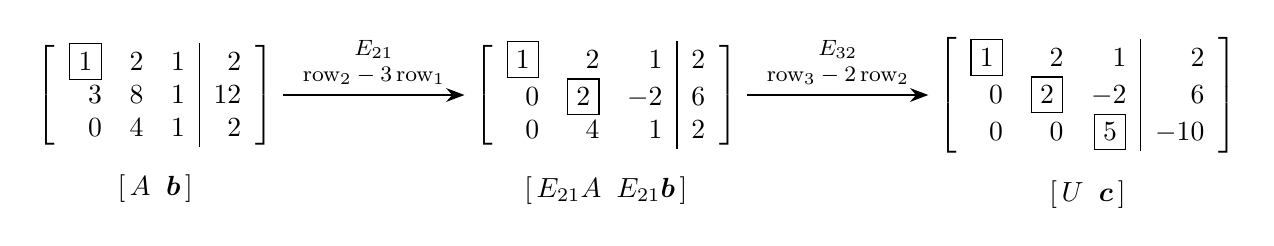
\begin{tikzpicture}[>=Stealth]
  \node (A) {$\left[\begin{array}{rrr|r} \boxed{1} & 2 & 1 & 2\\ 3 & 8 & 1 & 12\\ 0 & 4 & 1 & 2\end{array}\right]$};
  \node[right=2.3cm of A] (B) {$\left[\begin{array}{rrr|r} \boxed{1} & 2 & 1 & 2\\ 0 & \boxed{2} & -2 & 6\\ 0 & 4 & 1 & 2\end{array}\right]$};
  \node[right=2.3cm of B] (C) {$\left[\begin{array}{rrr|r} \boxed{1} & 2 & 1 & 2\\ 0 & \boxed{2} & -2 & 6\\ 0 & 0 & \boxed{5} & -10\end{array}\right]$};
  \draw[->,thick] (A) -- node[above,align=center,font=\footnotesize] {$E_{21}$\\ row$_2-3\,$row$_1$} (B);
  \draw[->,thick] (B) -- node[above,align=center,font=\footnotesize] {$E_{32}$\\ row$_3-2\,$row$_2$} (C);
  \node[below=3pt of A] {$[\,A\;\;\vb{b}\,]$};
  \node[below=3pt of B] {$[\,E_{21}A\;\;E_{21}\vb{b}\,]$};
  \node[below=3pt of C] {$[\,U\;\;\vb{c}\,]$};
\end{tikzpicture}
\caption{Forward elimination on the augmented matrix. Boxed entries are pivots. Each arrow is
one row operation, equivalently one multiplication on the left by an elimination matrix; the
step $E_{31}$ is skipped because the $(3,1)$ entry is already zero. The right-hand column
changes from $\vb{b}=(2,12,2)$ to $\vb{c}=(2,6,-10)$.}\label{fig:u03-flow}
\end{figure}

\subsection{Back substitution}

The triangular system $U\vb{x}=\vb{c}$ reads
\[
  x+2y+z=2,\qquad 2y-2z=6,\qquad 5z=-10 .
\]
Solve it in reverse order. The last equation gives $z=-2$. The second becomes
$2y+4=6$, so $y=1$. The first becomes $x+2-2=2$, so $x=2$. Checking in the original
equations \eqref{eq:u03-system}: $2+2-2=2$, $6+8-2=12$, $4-2=2$.

\begin{proposition}[Back substitution]\label{prop:u03-back}
Let $U$ be an $n\times n$ upper triangular matrix whose diagonal entries $u_{11},\dots,u_{nn}$
are all nonzero. Then for every $\vb{c}$ the system $U\vb{x}=\vb{c}$ has exactly one
solution, given by
\[
  x_n=\frac{c_n}{u_{nn}},\qquad
  x_i=\frac{1}{u_{ii}}\Bigl(c_i-\sum_{j=i+1}^{n}u_{ij}x_j\Bigr)\quad (i=n-1,\dots,1).
\]
\end{proposition}

\begin{proof}
Equation $i$ of $U\vb{x}=\vb{c}$ is $u_{ii}x_i+\sum_{j>i}u_{ij}x_j=c_i$, because the entries
left of the diagonal are zero. Equation $n$ involves only $x_n$ and forces $x_n=c_n/u_{nn}$.
Suppose $x_{i+1},\dots,x_n$ are already forced. Then equation $i$ has exactly one unknown
left, $x_i$, with the nonzero coefficient $u_{ii}$, so it forces the stated value. Working
upward, every component is forced, which proves uniqueness; and the values so obtained
satisfy every equation, which proves existence.
\end{proof}

\subsection{When elimination breaks down}

Zero is never allowed as a pivot. If a zero appears in the pivot position, there are two
cases.

\emph{Temporary failure.} If some row \emph{below} has a nonzero entry in that column,
exchange the two rows and continue.

\begin{example}[A row exchange rescues elimination]\label{ex:u03-exchange}
Change the $8$ in $A$ to a $6$. The first step gives
row~2 $=(3,6,1)-3(1,2,1)=(0,0,-2)$, a zero in the $(2,2)$ pivot position. Row~3 is
$(0,4,1)$, with a nonzero entry there, so exchange rows~2 and~3:
\[
  \begin{bmatrix} 1 & 2 & 1\\ 0 & 0 & -2\\ 0 & 4 & 1\end{bmatrix}
  \;\xrightarrow{\text{exchange rows 2, 3}}\;
  \begin{bmatrix} 1 & 2 & 1\\ 0 & 4 & 1\\ 0 & 0 & -2\end{bmatrix},
\]
which is already triangular, with pivots $1,4,-2$. The matrix is fine; only the order of the
equations was unlucky.
\end{example}

\emph{Complete failure.} If the pivot position holds a zero and every entry below it is zero
too, no exchange helps.

\begin{example}[Elimination fails: a singular matrix]\label{ex:u03-singular}
Change the $(3,3)$ entry of $A$ from $1$ to $-4$. The first step
gives row~2 $=(0,2,-2)$ and leaves row~3 $=(0,4,-4)$; subtracting $2$ times row~2 leaves
row~3 $=(0,0,0)$. There is no third pivot. The matrix is \emph{singular}: depending on
$\vb{b}$, the system has no solution or infinitely many, never exactly one. (In the column
picture, column~3 has become $(1,1,-4)=3\,(1,3,0)-(2,8,4)$, a combination of the
first two columns.)
\end{example}

In summary, elimination on an $n\times n$ matrix proceeds as follows.
\begin{enumerate}
  \item For $k=1,\dots,n$: if the $(k,k)$ entry is zero, exchange row $k$ with a lower row
    that has a nonzero entry in column $k$; if there is none, stop: $A$ is singular.
  \item For each row $i>k$, compute $\ell_{ik}=a_{ik}/a_{kk}$ (current entries) and subtract
    $\ell_{ik}$ times row $k$ from row $i$, in the augmented column as well.
  \item When all $n$ pivots are found, solve $U\vb{x}=\vb{c}$ by back substitution.
\end{enumerate}

\begin{trap}
The multipliers use the \emph{current} entries, not the original ones: in step $(3,2)$ the
multiplier is $4/2$, where $2$ is the pivot created by step $(2,1)$, not the original entry
$8$. And a zero in a pivot position is not yet a verdict of singularity: look below it first.
Only a zero with nothing nonzero underneath means failure.
\end{trap}

\subsection{Each elimination step is a matrix}

To put elimination into matrix language we need products of matrices. Multiplying a matrix
by a column gives a combination of its columns (Definition~\ref{def:u01-Ax}). The mirror image
is a row times a matrix.

\begin{proposition}[Row times matrix]\label{prop:u03-rowtimes}
If $\vb{y}\T=(y_1,\dots,y_m)$ is a row vector and $A$ is $m\times n$ with rows
$\vb{r}_1,\dots,\vb{r}_m$, then $\vb{y}\T A=y_1\vb{r}_1+\cdots+y_m\vb{r}_m$, a combination of
the rows of $A$.
\end{proposition}

\begin{proof}
Entry $j$ of $\vb{y}\T A$ is the row $\vb{y}\T$ times column $j$ of $A$, namely
$\sum_i y_ia_{ij}$. Entry $j$ of $\sum_i y_i\vb{r}_i$ is also $\sum_i y_ia_{ij}$, since
$a_{ij}$ is entry $j$ of row $\vb{r}_i$.
\end{proof}

For example, $\begin{bmatrix} 1 & 2 & 7\end{bmatrix}A
=1\,(1,2,1)+2\,(3,8,1)+7\,(0,4,1)=(7,46,10)$.
For a matrix $E$ with $m$ columns and a matrix $A$ with $m$ rows, the product $EA$ is the
matrix whose column $j$ is $E$ times column $j$ of $A$; its $(i,j)$ entry is row $i$ of $E$
times column $j$ of $A$. By Proposition~\ref{prop:u03-rowtimes}, \emph{row $i$ of $EA$ is
the combination of the rows of $A$ given by row $i$ of $E$}. (Section~\ref{sec:u04} collects
all the ways to see a matrix product.) So to subtract $3$ times row~1 from row~2 and leave
the other rows alone, the rows of $E$ must be $(1,0,0)$, $(-3,1,0)$ and $(0,0,1)$.

\begin{definition}[Elimination matrix]\label{def:u03-Eij}
For $i\neq j$, the \emph{elimination matrix} $E_{ij}$ with multiplier $\ell$ is the identity
matrix with the entry $-\ell$ placed in row $i$, column $j$. Multiplying on the left,
$E_{ij}A$ subtracts $\ell$ times row $j$ of $A$ from row $i$ and leaves the other rows
unchanged.
\end{definition}

\begin{example}[Elimination as matrix multiplication]\label{ex:u03-matrices}
For the example \eqref{eq:u03-system}, the two nontrivial steps are
\[
  E_{21}=\begin{bmatrix} 1 & 0 & 0\\ -3 & 1 & 0\\ 0 & 0 & 1\end{bmatrix},\qquad
  E_{32}=\begin{bmatrix} 1 & 0 & 0\\ 0 & 1 & 0\\ 0 & -2 & 1\end{bmatrix}.
\]
Then
\[
  E_{21}A=\begin{bmatrix} 1 & 2 & 1\\ 0 & 2 & -2\\ 0 & 4 & 1\end{bmatrix},\qquad
  E_{32}(E_{21}A)=\begin{bmatrix} 1 & 2 & 1\\ 0 & 2 & -2\\ 0 & 0 & 5\end{bmatrix}=U.
\]
Spot-check one entry: the $(2,3)$ entry of $E_{21}A$ is row~2 of $E_{21}$ times column~3 of
$A$, $(-3)(1)+(1)(1)+(0)(1)=-2$. The step $E_{31}$ is the identity, because $\ell_{31}=0$.
\end{example}

The whole of forward elimination is the single line $E_{32}(E_{31}(E_{21}A))=U$. Can we
multiply the $E$'s together first, to get one matrix that does everything? Yes, because
matrix multiplication is associative.

\begin{proposition}[Associative law]\label{prop:u03-assoc}
If the shapes allow the products, $(EF)A=E(FA)$.
\end{proposition}

\begin{proof}
Compare the $(i,j)$ entries, writing $e,f,a$ for the entries of $E,F,A$:
\[
  \bigl((EF)A\bigr)_{ij}=\sum_k\Bigl(\sum_l e_{il}f_{lk}\Bigr)a_{kj}
  =\sum_l e_{il}\Bigl(\sum_k f_{lk}a_{kj}\Bigr)=\bigl(E(FA)\bigr)_{ij}.
\]
Both are the sum of $e_{il}f_{lk}a_{kj}$ over all $k$ and $l$, added in a different order.
\end{proof}

So we may move parentheses freely, as long as the order of the factors is kept. For the
example, $E=E_{32}E_{21}$ does all of elimination at once:
\[
  E=\begin{bmatrix} 1 & 0 & 0\\ 0 & 1 & 0\\ 0 & -2 & 1\end{bmatrix}
  \begin{bmatrix} 1 & 0 & 0\\ -3 & 1 & 0\\ 0 & 0 & 1\end{bmatrix}
  =\begin{bmatrix} 1 & 0 & 0\\ -3 & 1 & 0\\ 6 & -2 & 1\end{bmatrix},\qquad EA=U,\quad E\vb{b}=\vb{c}.
\]
The entry $6$ appears because $3$ of row~1 went into row~2 and then $2$ of that row~2 went into
row~3. Section~\ref{sec:u05} shows how to avoid such entries by recording elimination the
other way around.

The order of the factors cannot be changed: the \emph{commutative} law fails for matrices.
Row exchanges show this vividly.

\begin{definition}[Permutation matrix]\label{def:u03-perm}
A \emph{permutation matrix} $P$ is the identity matrix with its rows reordered. Multiplying
on the left, $PA$ reorders the rows of $A$ in the same way.
\end{definition}

To exchange the two rows of a $2\times2$ matrix, exchange the rows of $I$:
\[
  \begin{bmatrix} 0 & 1\\ 1 & 0\end{bmatrix}\begin{bmatrix} a & b\\ c & d\end{bmatrix}
  =\begin{bmatrix} c & d\\ a & b\end{bmatrix},
  \qquad
  \begin{bmatrix} a & b\\ c & d\end{bmatrix}\begin{bmatrix} 0 & 1\\ 1 & 0\end{bmatrix}
  =\begin{bmatrix} b & a\\ d & c\end{bmatrix}.
\]
On the left, $P$ acts on rows; on the right, the same $P$ acts on columns (each column of $AP$
is a combination of the columns of $A$). So $PA\neq AP$ in general. In elimination we use
row operations, so the elimination and permutation matrices always multiply from the left.

\subsection{Undoing a step: inverse matrices}

Every elimination step can be undone. If $E_{21}$ subtracts $3$ times row~1 from row~2, the
step that brings row~2 back adds $3$ times row~1 to row~2:
\[
  E_{21}^{-1}E_{21}=
  \begin{bmatrix} 1 & 0 & 0\\ 3 & 1 & 0\\ 0 & 0 & 1\end{bmatrix}
  \begin{bmatrix} 1 & 0 & 0\\ -3 & 1 & 0\\ 0 & 0 & 1\end{bmatrix}
  =\begin{bmatrix} 1 & 0 & 0\\ 0 & 1 & 0\\ 0 & 0 & 1\end{bmatrix}=I .
\]
For example, $E_{21}$ turns $\vb{b}=(2,12,2)$ into $(2,6,2)$, and $E_{21}^{-1}$ turns
$(2,6,2)$ back into $(2,12,2)$. The matrix $I$ is the \emph{identity}: $I\vb{x}=\vb{x}$ for
every $\vb{x}$, the matrix analogue of the number $1$.

\begin{proposition}[Inverse of an elimination matrix]\label{prop:u03-Einv}
Let $E_{ij}(\ell)$ denote the elimination matrix with $-\ell$ in position $(i,j)$. Then
$E_{ij}(-\ell)\,E_{ij}(\ell)=I=E_{ij}(\ell)\,E_{ij}(-\ell)$. A permutation matrix that
exchanges two rows is its own inverse.
\end{proposition}

\begin{proof}
Apply $E_{ij}(-\ell)E_{ij}(\ell)$ to any matrix $M$. The first factor replaces row $i$ by
(row $i$) $-\ell\,$(row $j$) and leaves row $j$ untouched, since $j\neq i$. The second factor
adds $\ell\,$(row $j$) back to row $i$, restoring $M$. A matrix that leaves every $M$
unchanged is $I$ (take $M=I$). The other order is the same argument with $\ell$ replaced by
$-\ell$. Exchanging the same two rows twice restores every matrix.
\end{proof}

This is why elimination is legitimate: with $E$ the product of all the step matrices,
$A\vb{x}=\vb{b}$ and $U\vb{x}=\vb{c}$ have the same solutions. If $A\vb{x}=\vb{b}$ then
$EA\vb{x}=E\vb{b}$, that is, $U\vb{x}=\vb{c}$. Conversely, each step can be reversed, so
multiplying $U\vb{x}=\vb{c}$ on the left by the inverse steps returns $A\vb{x}=\vb{b}$. The
answer $\vb{x}=(2,1,-2)$ found by back substitution is therefore the solution of the original
system.

\begin{trap}
Row operations multiply on the \emph{left}; a matrix on the right of $A$ combines columns.
Writing $AE_{21}$ instead of $E_{21}A$ subtracts $3$ times column~2 from column~1, a
different operation entirely. Also keep the factors in order: elimination is $E_{32}E_{21}A$,
not $E_{21}E_{32}A$.
\end{trap}

\subsection{Exercises}

\begin{exercise}\label{ex:u03-two}
For the system $2x+3y=5$, $6x+15y=12$: what multiple of equation~1 should be subtracted from
equation~2? Write the system as $A\vb{x}=\vb{b}$, eliminate (what are the pivots?), and solve by
back substitution. Check your answer in both equations.
\end{exercise}
\begin{solution}
Subtract $\ell_{21}=6/2=3$ times equation~1. In matrix form,
\[
  \begin{bmatrix} 2 & 3\\ 6 & 15\end{bmatrix}\begin{bmatrix} x\\ y\end{bmatrix}
  =\begin{bmatrix} 5\\ 12\end{bmatrix}
  \;\longrightarrow\;
  \begin{bmatrix} 2 & 3\\ 0 & 6\end{bmatrix}\begin{bmatrix} x\\ y\end{bmatrix}
  =\begin{bmatrix} 5\\ -3\end{bmatrix},
\]
since $15-3\cdot3=6$ and $12-3\cdot5=-3$. The pivots are $2$ and $6$. Back substitution:
$6y=-3$ gives $y=-\tfrac12$; then $2x-\tfrac32=5$ gives $x=\tfrac{13}{4}$. Check:
$2\cdot\tfrac{13}{4}+3(-\tfrac12)=\tfrac{13}{2}-\tfrac32=5$ and
$6\cdot\tfrac{13}{4}+15(-\tfrac12)=\tfrac{39}{2}-\tfrac{15}{2}=12$.
\end{solution}

\begin{exercise}\label{ex:u03-four}
Solve by elimination, using a row exchange when needed:
\[
  x-y-z+u=0,\qquad 2x+2z=8,\qquad -y-2z=-8,\qquad 3x-3y-2z+4u=7 .
\]
\end{exercise}
\begin{solution}
The augmented matrix and the elimination steps:
\[
  \left[\begin{array}{rrrr|r} 1&-1&-1&1&0\\ 2&0&2&0&8\\ 0&-1&-2&0&-8\\ 3&-3&-2&4&7\end{array}\right]
  \to
  \left[\begin{array}{rrrr|r} 1&-1&-1&1&0\\ 0&2&4&-2&8\\ 0&-1&-2&0&-8\\ 0&0&1&1&7\end{array}\right]
  \to
  \left[\begin{array}{rrrr|r} 1&-1&-1&1&0\\ 0&2&4&-2&8\\ 0&0&0&-1&-4\\ 0&0&1&1&7\end{array}\right].
\]
The first arrow subtracts $2$ times row~1 from row~2 and $3$ times row~1 from row~4. The
second adds $\tfrac12$ of row~2 to row~3 (multiplier $\ell_{32}=-\tfrac12$). Now the $(3,3)$
position holds $0$, but row~4 has a $1$ below it, so exchange rows~3 and~4; the matrix is
then upper triangular with pivots $1,2,1,-1$. Back substitution: $-u=-4$ gives $u=4$;
$z+u=7$ gives $z=3$; $2y+4z-2u=8$ gives $2y=8-12+8=4$, $y=2$; $x-y-z+u=0$ gives $x=2+3-4=1$.
So $(x,y,z,u)=(1,2,3,4)$. Check the last equation: $3-6-6+16=7$.
\end{solution}

\begin{exercise}\label{ex:u03-pascal}
Find the lower triangular $E$ that reduces the $4\times4$ Pascal matrix to a smaller Pascal
matrix:
\[
  E\begin{bmatrix} 1&0&0&0\\ 1&1&0&0\\ 1&2&1&0\\ 1&3&3&1\end{bmatrix}
  =\begin{bmatrix} 1&0&0&0\\ 0&1&0&0\\ 0&1&1&0\\ 0&1&2&1\end{bmatrix}.
\]
Which matrix $M$, a product of several such $E$'s, reduces the Pascal matrix all the way to $I$?
\end{exercise}
\begin{solution}
Subtracting each row from the row below it uses Pascal's rule
$\binom{i}{j}-\binom{i-1}{j}=\binom{i-1}{j-1}$ and produces the smaller Pascal matrix:
\[
  E=\begin{bmatrix} 1&0&0&0\\ -1&1&0&0\\ 0&-1&1&0\\ 0&0&-1&1\end{bmatrix}.
\]
(Here row $i$ is replaced by row $i$ minus the \emph{original} row $i-1$; as a sequence of
elimination steps, do row~4 first, then row~3, then row~2.) The same idea one level down
clears the second column with $E_2$ (rows~3 and~4 minus the rows above them, leaving rows~1,
2 alone), and then $E_3$ subtracts row~3 from row~4:
\[
  E_2=\begin{bmatrix} 1&0&0&0\\ 0&1&0&0\\ 0&-1&1&0\\ 0&0&-1&1\end{bmatrix},\quad
  E_3=\begin{bmatrix} 1&0&0&0\\ 0&1&0&0\\ 0&0&1&0\\ 0&0&-1&1\end{bmatrix},\quad
  M=E_3E_2E=\begin{bmatrix} 1&0&0&0\\ -1&1&0&0\\ 1&-2&1&0\\ -1&3&-3&1\end{bmatrix}.
\]
Since $M$ times the Pascal matrix is $I$, $M$ is its inverse: Pascal's triangle with
alternating signs.
\end{solution}

\begin{exercise}\label{ex:u03-fail}
For which numbers $d$ does elimination on
$A=\begin{bmatrix} 2&1&0\\ 4&d&1\\ 0&1&2\end{bmatrix}$ meet a zero in a pivot position? For
each such $d$, say whether a row exchange rescues it.
\end{exercise}
\begin{solution}
The first pivot is $2$; subtracting $2$ times row~1 from row~2 gives row~2 $=(0,\,d-2,\,1)$.
If $d=2$ the $(2,2)$ position is zero, but row~3 $=(0,1,2)$ has a $1$ below it; exchanging
rows~2 and~3 gives pivots $2,1,1$ (the matrix becomes $\begin{bmatrix}2&1&0\\0&1&2\\0&0&1\end{bmatrix}$),
so this failure is only temporary. If $d\neq2$, the second pivot is $d-2$; the multiplier is
$\ell_{32}=1/(d-2)$, and the third pivot is $2-\frac{1}{d-2}$. It is zero when $d-2=\tfrac12$,
that is $d=\tfrac52$, and then nothing lies below it: complete failure, and $A$ is singular.
For every other $d$, elimination succeeds without exchanges.
\end{solution}

% unit: u04
% sources: sources/080-multiplication-and-inverse-matrices.txt, sources/127-multiplication-and-inverse-matrices.txt, sources/128-mit18-06scf11-ses1-3sum-pdf-download-file.txt, sources/129-inverse-matrices.txt, sources/130-mit18-06scf11-ses1-3prob-pdf-download-file.txt, sources/131-mit18-06scf11-ses1-3sol-pdf-download-file.txt
\section{Multiplication and inverse matrices}\label{sec:u04}

We have been multiplying matrices since Section~\ref{sec:u03}, where elimination steps were
matrices acting on the left. This section sets down the rule for the product $AB$ and then
looks at the same product in four more ways: by columns, by rows, as a sum of
column-times-row pieces, and by blocks. All five give the same answer, and each is the right
one in some argument later on. The second half answers the most important question about a
square matrix: does it have an inverse? A singular matrix sends some nonzero vector to zero,
which no inverse can undo; for an invertible matrix, Gauss--Jordan elimination computes
$A^{-1}$.

\subsection{The rule: row times column}

\begin{definition}[Matrix product]\label{def:u04-product}
Let $A$ be $m\times n$ and $B$ be $n\times p$. The product $C=AB$ is the $m\times p$ matrix
with entries
\[
  c_{ij}=\sum_{k=1}^{n}a_{ik}b_{kj}=a_{i1}b_{1j}+a_{i2}b_{2j}+\cdots+a_{in}b_{nj},
\]
the dot product of row $i$ of $A$ with column $j$ of $B$. The product is defined only when
the number of columns of $A$ equals the number of rows of $B$.
\end{definition}

For instance, the entry $c_{34}$ comes from row~3 of $A$ and column~4 of $B$:
$c_{34}=a_{31}b_{14}+a_{32}b_{24}+\cdots+a_{3n}b_{n4}$. The shapes follow the pattern
$(m\times n)(n\times p)=(m\times p)$: the inner numbers must match and disappear, the outer
numbers give the shape. When $B$ is a single column ($p=1$), this is the row form of
$A\vb{x}$ from Proposition~\ref{prop:u01-rows}.

\subsection{Columns, rows, and columns times rows}

The entry rule hides what the product does to whole vectors. The next three views each look at
whole columns or rows.

\begin{proposition}[Three more views of $AB$]\label{prop:u04-views}
Let $A$ be $m\times n$ with columns $\vb{a}_1,\dots,\vb{a}_n$ and let $B$ be $n\times p$ with
columns $\vb{b}_1,\dots,\vb{b}_p$ and rows $\vb{r}_1\T,\dots,\vb{r}_n\T$.
\begin{enumerate}[(a)]
  \item \emph{Columns:} column $j$ of $AB$ is $A\vb{b}_j$. Every column of $AB$ is a
    combination of the columns of $A$.
  \item \emph{Rows:} row $i$ of $AB$ is (row $i$ of $A$) times $B$. Every row of $AB$ is a
    combination of the rows of $B$.
  \item \emph{Columns times rows:} $AB=\vb{a}_1\vb{r}_1\T+\vb{a}_2\vb{r}_2\T+\cdots+\vb{a}_n\vb{r}_n\T$,
    a sum of $n$ matrices, each an $m\times1$ column times a $1\times p$ row.
\end{enumerate}
\end{proposition}

\begin{proof}
(a) The entries of $A\vb{b}_j$ are $\sum_k a_{ik}b_{kj}$ for $i=1,\dots,m$
(Proposition~\ref{prop:u01-rows}), which is column $j$ of $AB$. By
Definition~\ref{def:u01-Ax}, $A\vb{b}_j=b_{1j}\vb{a}_1+\cdots+b_{nj}\vb{a}_n$.
(b) Entry $j$ of (row $i$ of $A$)$\,B$ is $\sum_k a_{ik}b_{kj}=c_{ij}$, and by
Proposition~\ref{prop:u03-rowtimes} that row is $a_{i1}\vb{r}_1\T+\cdots+a_{in}\vb{r}_n\T$.
(c) The column-times-row product $\vb{a}_k\vb{r}_k\T$ is the $m\times p$ matrix with $(i,j)$
entry $a_{ik}b_{kj}$. Summing over $k$ gives $\sum_k a_{ik}b_{kj}=c_{ij}$.
\end{proof}

\begin{example}[One product, four ways]\label{ex:u04-four-ways}
Let $A=\begin{bmatrix} 1 & 2\\ 3 & 4\end{bmatrix}$ ($2\times2$) and
$B=\begin{bmatrix} 1 & 0 & 2\\ 1 & 1 & 0\end{bmatrix}$ ($2\times3$), so $AB$ is $2\times3$.
\begin{itemize}
  \item \emph{Entries.} $c_{23}=(3,4)\cdot(2,0)=6$; similarly for the other five entries.
  \item \emph{Columns.} $A(1,1)=(1+2,\,3+4)=(3,7)$, $A(0,1)=(2,4)$, $A(2,0)=(2,6)$.
  \item \emph{Rows.} $(1,2)B=1\,(1,0,2)+2\,(1,1,0)=(3,2,2)$ and
    $(3,4)B=3\,(1,0,2)+4\,(1,1,0)=(7,4,6)$.
  \item \emph{Columns times rows.}
    \[
      \begin{bmatrix} 1\\ 3\end{bmatrix}\begin{bmatrix} 1 & 0 & 2\end{bmatrix}
      +\begin{bmatrix} 2\\ 4\end{bmatrix}\begin{bmatrix} 1 & 1 & 0\end{bmatrix}
      =\begin{bmatrix} 1 & 0 & 2\\ 3 & 0 & 6\end{bmatrix}
      +\begin{bmatrix} 2 & 2 & 0\\ 4 & 4 & 0\end{bmatrix}.
    \]
\end{itemize}
Every view gives $AB=\begin{bmatrix} 3 & 2 & 2\\ 7 & 4 & 6\end{bmatrix}$. The
same twelve multiplications are being done each time; only the grouping changes.
\end{example}

A single column times a single row is a very special matrix:
\[
  \begin{bmatrix} 2\\ 3\\ 4\end{bmatrix}\begin{bmatrix} 1 & 6\end{bmatrix}
  =\begin{bmatrix} 2 & 12\\ 3 & 18\\ 4 & 24\end{bmatrix}.
\]
Its columns are multiples of $(2,3,4)$ and its rows are multiples of $(1,6)$, as views (a)
and (b) predict. Plotted as points, the rows $(2,12)$, $(3,18)$, $(4,24)$ all lie on the line
through $(1,6)$, and both columns lie on the line through $(2,3,4)$. In later language
(Section~\ref{sec:u11}), its row space and column space are both lines: it is a matrix of
rank one. View (c) says that every product $AB$ is a sum of such rank-one pieces. For
instance, if $A$ has columns $(2,3,4)$ and $(7,8,9)$ and $B$ has rows $(1,6)$ and $(0,0)$,
the second piece is zero and $AB$ is the matrix above.

\subsection{Block multiplication}

Matrices can be cut into blocks, and if the cuts match, blocks multiply like numbers
(keeping their order). With $A$ and $B$ cut into $2\times2$ arrays of blocks,
\[
  \begin{bmatrix} A_1 & A_2\\ A_3 & A_4\end{bmatrix}
  \begin{bmatrix} B_1 & B_2\\ B_3 & B_4\end{bmatrix}
  =\begin{bmatrix} A_1B_1+A_2B_3 & A_1B_2+A_2B_4\\ A_3B_1+A_4B_3 & A_3B_2+A_4B_4\end{bmatrix},
\]
provided the columns of $A$ are cut the same way as the rows of $B$, so that every product
$A_iB_j$ is defined.

\begin{proposition}[Block multiplication]\label{prop:u04-blocks}
If the column partition of $A$ matches the row partition of $B$, then block $(I,J)$ of $AB$
is $\sum_K A_{IK}B_{KJ}$, a sum of block products.
\end{proposition}

\begin{proof}
Take an entry $c_{ij}$ inside block $(I,J)$. Its sum $\sum_k a_{ik}b_{kj}$ runs over all
column indices $k$ of $A$. Split this sum according to the column blocks $K$: the part with
$k$ in block $K$ is exactly the $(i,j)$ entry of $A_{IK}B_{KJ}$. Adding over $K$ gives the
claim.
\end{proof}

\begin{example}[Blocks behave like numbers]\label{ex:u04-blocks}
Let $C=\begin{bmatrix} 1 & 2\\ 3 & 4\end{bmatrix}$ and let $I$, $0$ be the $2\times2$ identity
and zero matrices. By block multiplication,
\[
  \begin{bmatrix} I & 0\\ C & I\end{bmatrix}\begin{bmatrix} I & 0\\ -C & I\end{bmatrix}
  =\begin{bmatrix} I\cdot I+0\cdot(-C) & I\cdot0+0\cdot I\\ C\cdot I+I\cdot(-C) & C\cdot 0+I\cdot I\end{bmatrix}
  =\begin{bmatrix} I & 0\\ 0 & I\end{bmatrix}.
\]
So the $4\times4$ matrix $\begin{bmatrix} I & 0\\ C & I\end{bmatrix}$, which adds combinations
of rows~1--2 to rows~3--4, is undone by subtracting the same combinations, exactly like the
elimination matrices of Proposition~\ref{prop:u03-Einv}.
\end{example}

Matrix multiplication obeys the associative law (Proposition~\ref{prop:u03-assoc}) and the
distributive laws $A(B+C)=AB+AC$, $(A+B)C=AC+BC$ (Exercise~\ref{ex:u04-distributive}), but
in general $AB\neq BA$.

\subsection{Inverse matrices}

\begin{definition}[Inverse, invertible, singular]\label{def:u04-inverse}
A square $n\times n$ matrix $A$ is \emph{invertible} (or \emph{nonsingular}) if there is an
$n\times n$ matrix $A^{-1}$ with
\[
  A^{-1}A=I\qquad\text{and}\qquad AA^{-1}=I .
\]
A square matrix with no inverse is \emph{singular}.
\end{definition}

An inverse, when it exists, is unique: if $BA=I$ and $AC=I$, then
$B=B(AC)=(BA)C=C$. For square matrices it is enough to find a one-sided inverse
(Corollary~\ref{cor:u04-onesided} below). (A rectangular matrix can have an inverse on one side only, as
Section~\ref{sec:u36} explains.)

Whether $A$ is invertible is the first question to ask about a square matrix. The clearest
way to see that a matrix is \emph{not} invertible is to find a vector it sends to zero.

\begin{theorem}[A nonzero solution of $A\vb{x}=\vb{0}$ rules out an inverse]\label{thm:u04-singular}
If $A$ is square and $A\vb{x}=\vb{0}$ for some $\vb{x}\neq\vb{0}$, then $A$ is singular.
\end{theorem}

\begin{proof}
Suppose $A^{-1}$ existed. Multiplying $A\vb{x}=\vb{0}$ on the left by $A^{-1}$ gives
$\vb{x}=A^{-1}A\vb{x}=A^{-1}\vb{0}=\vb{0}$, contradicting $\vb{x}\neq\vb{0}$.
\end{proof}

\begin{example}[A singular matrix, three ways]\label{ex:u04-singular}
Take $A=\begin{bmatrix} 1 & 3\\ 2 & 6\end{bmatrix}$.
\emph{Null vector:} $\vb{x}=(3,-1)$ gives $A\vb{x}=3(1,2)-1(3,6)=(0,0)$, so $A$ is singular
by Theorem~\ref{thm:u04-singular}.
\emph{Columns:} column~2 is $3$ times column~1, so both columns lie on the line through
$(1,2)$. By Proposition~\ref{prop:u04-views}(a), every column of any product $AB$ lies on that
line too, so $AB$ can never have the column $(1,0)$ of $I$.
\emph{Elimination:} subtracting $2$ times row~1 from row~2 leaves $(0,0)$, so there is no
second pivot. (For readers who know determinants: $1\cdot6-3\cdot2=0$.)
\end{example}

\begin{figure}[ht]
\centering
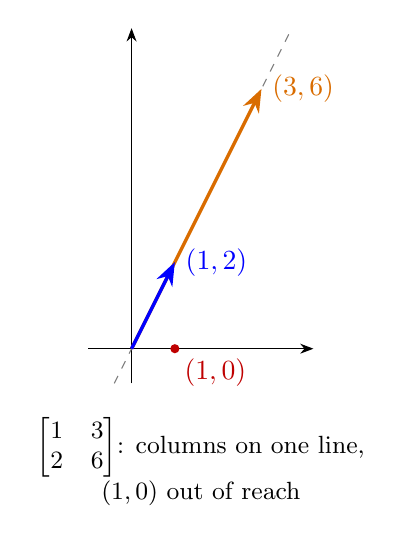
\begin{tikzpicture}[scale=0.55,>=Stealth]
  \draw[->] (-1,0) -- (4.2,0);
  \draw[->] (0,-0.8) -- (0,7.4);
  \draw[dashed,gray] (-0.4,-0.8) -- (3.7,7.4);
  \draw[->,very thick,orange!85!black] (0,0) -- (3,6) node[right] {$(3,6)$};
  \draw[->,very thick,blue] (0,0) -- (1,2) node[right] {$(1,2)$};
  \fill[red!75!black] (1,0) circle (3pt) node[below right] {$(1,0)$};
  \node[font=\small,align=center] at (1.6,-2.6) {$\begin{bmatrix} 1&3\\ 2&6\end{bmatrix}$: columns on one line,\\ $(1,0)$ out of reach};
\end{tikzpicture}
\qquad\qquad
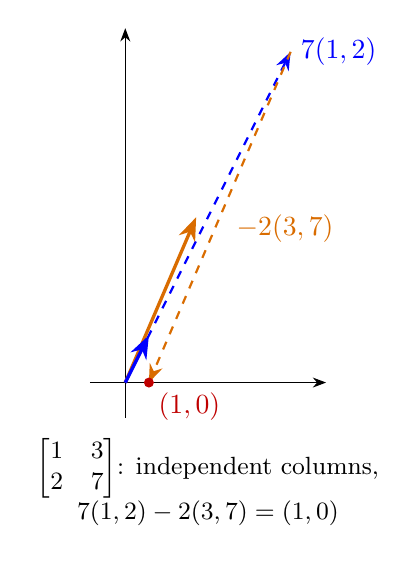
\begin{tikzpicture}[scale=0.3,>=Stealth]
  \draw[->] (-1.5,0) -- (8.5,0);
  \draw[->] (0,-1.5) -- (0,15);
  \draw[->,thick,dashed,blue] (0,0) -- (7,14) node[right] {$7(1,2)$};
  \draw[->,thick,dashed,orange!85!black] (7,14) -- (1,0);
  \node[orange!85!black,right] at (4.3,6.5) {$-2(3,7)$};
  \draw[->,very thick,orange!85!black] (0,0) -- (3,7);
  \draw[->,very thick,blue] (0,0) -- (1,2);
  \fill[red!75!black] (1,0) circle (6pt) node[below right] {$(1,0)$};
  \node[font=\small,align=center] at (3.5,-4.2) {$\begin{bmatrix} 1&3\\ 2&7\end{bmatrix}$: independent columns,\\ $7(1,2)-2(3,7)=(1,0)$};
\end{tikzpicture}
\caption{Left: the columns of the singular matrix lie on one line (dashed), so every
combination stays on it and the column $(1,0)$ of $I$ cannot be produced. Right: the columns
$(1,2)$ and $(3,7)$ of the invertible matrix (solid, near the origin) point in different
directions, so their combinations fill the plane. Seven copies of the first column followed
by $-2$ copies of the second (dashed) land on $(1,0)$; the weights $7,-2$ form the first column
of $A^{-1}$. They are large because the two columns are nearly parallel.}
\label{fig:u04-columns}
\end{figure}

\subsection{Gauss--Jordan elimination computes \texorpdfstring{\(A^{-1}\)}{the inverse}}

Now change the $6$ to a $7$: $A=\begin{bmatrix} 1 & 3\\ 2 & 7\end{bmatrix}$. Its columns point
in different directions (Figure~\ref{fig:u04-columns}), and we look for
$A^{-1}=\begin{bmatrix} a & c\\ b & d\end{bmatrix}$ with $AA^{-1}=I$. By the column view,
this is two systems with the same matrix:
\[
  A\begin{bmatrix} a\\ b\end{bmatrix}=\begin{bmatrix} 1\\ 0\end{bmatrix},\qquad
  A\begin{bmatrix} c\\ d\end{bmatrix}=\begin{bmatrix} 0\\ 1\end{bmatrix}.
\]
In general, column $j$ of $A^{-1}$ solves $A\vb{x}=\vb{e}_j$, where $\vb{e}_j$ is column $j$
of $I$. Finding $A^{-1}$ means solving $n$ systems at once. Gauss's elimination would solve
them one at a time; Jordan's idea is to carry all $n$ right-hand sides along as extra columns
and keep eliminating \emph{upwards} until the left half is $I$.

\begin{example}[Gauss--Jordan on a $2\times2$ matrix]\label{ex:u04-gj2}
\[
  \left[\begin{array}{rr|rr} 1 & 3 & 1 & 0\\ 2 & 7 & 0 & 1\end{array}\right]
  \xrightarrow{\ \text{row}_2-2\,\text{row}_1\ }
  \left[\begin{array}{rr|rr} 1 & 3 & 1 & 0\\ 0 & 1 & -2 & 1\end{array}\right]
  \xrightarrow{\ \text{row}_1-3\,\text{row}_2\ }
  \left[\begin{array}{rr|rr} 1 & 0 & 7 & -3\\ 0 & 1 & -2 & 1\end{array}\right].
\]
The first step is ordinary elimination (Gauss stops at the upper triangular form). The second
clears the entry \emph{above} the pivot (Jordan continues). The right half is
$A^{-1}=\begin{bmatrix} 7 & -3\\ -2 & 1\end{bmatrix}$. Check:
$A^{-1}A=\begin{bmatrix} 7-6 & 21-21\\ -2+2 & -6+7\end{bmatrix}=I$.
\end{example}

\begin{theorem}[Why Gauss--Jordan works]\label{thm:u04-gj}
Suppose a sequence of row operations (elimination steps, row exchanges, and division of rows
by nonzero pivots) turns $[\,A\;\;I\,]$ into $[\,I\;\;E\,]$. Then $E=A^{-1}$: both $EA=I$
and $AE=I$.
\end{theorem}

\begin{proof}
Each row operation is multiplication on the left by an invertible matrix (an elimination
matrix, a permutation, or a diagonal matrix with one nonzero entry changed), so the whole
sequence is multiplication by their product, call it $M$. By block multiplication
$M[\,A\;\;I\,]=[\,MA\;\;M\,]$, and this equals $[\,I\;\;E\,]$. So $M=E$ and $EA=I$.
Moreover $M$ is invertible, its inverse being the product of the inverse steps in reverse
order. Hence $A=M^{-1}(MA)=M^{-1}$, and $AE=M^{-1}M=I$.
\end{proof}

\begin{example}[A $3\times3$ inverse]\label{ex:u04-gj3}
Invert $K=\begin{bmatrix} 2 & -1 & 0\\ -1 & 2 & -1\\ 0 & -1 & 2\end{bmatrix}$. Forward
elimination (multipliers $-\tfrac12$, then $-\tfrac23$):
{\renewcommand{\arraystretch}{1.3}
\[
  \left[\begin{array}{rrr|rrr} 2&-1&0&1&0&0\\ -1&2&-1&0&1&0\\ 0&-1&2&0&0&1\end{array}\right]
  \to
  \left[\begin{array}{rrr|rrr} 2&-1&0&1&0&0\\ 0&\tfrac32&-1&\tfrac12&1&0\\ 0&0&\tfrac43&\tfrac13&\tfrac23&1\end{array}\right].
\]}%
Upward elimination: add $\tfrac34$ of row~3 to row~2, then $\tfrac23$ of the new row~2 to
row~1; finally divide by the pivots $2,\tfrac32,\tfrac43$:
{\renewcommand{\arraystretch}{1.3}
\[
  \to
  \left[\begin{array}{rrr|rrr} 2&0&0&\tfrac32&1&\tfrac12\\ 0&\tfrac32&0&\tfrac34&\tfrac32&\tfrac34\\ 0&0&\tfrac43&\tfrac13&\tfrac23&1\end{array}\right]
  \to
  \left[\begin{array}{rrr|rrr} 1&0&0&\tfrac34&\tfrac12&\tfrac14\\ 0&1&0&\tfrac12&1&\tfrac12\\ 0&0&1&\tfrac14&\tfrac12&\tfrac34\end{array}\right].
\]}%
So $K^{-1}=\frac14\begin{bmatrix} 3&2&1\\ 2&4&2\\ 1&2&3\end{bmatrix}$. Notice that $K$ is
symmetric and so is $K^{-1}$, and that $K^{-1}$ has no zero entries although $K$ has two.
\end{example}

Putting the pieces together gives the basic test for invertibility of a square matrix.

\begin{theorem}[Invertibility test]\label{thm:u04-test}
For an $n\times n$ matrix $A$ the following are equivalent:
\begin{enumerate}[(a)]
  \item $A$ is invertible;
  \item $A\vb{x}=\vb{0}$ has only the solution $\vb{x}=\vb{0}$;
  \item elimination, with row exchanges allowed, produces $n$ nonzero pivots.
\end{enumerate}
\end{theorem}

\begin{proof}
(a)$\Rightarrow$(b) is Theorem~\ref{thm:u04-singular}. (c)$\Rightarrow$(a): with $n$ pivots,
continue upward and divide by the pivots; this is Gauss--Jordan, and
Theorem~\ref{thm:u04-gj} produces $A^{-1}$. (b)$\Rightarrow$(c): suppose elimination stops at
column $k$ because the entries of the current matrix $M$ in column $k$, from row $k$ down, are
all zero. The first $k-1$ columns of $M$ have pivots in rows $1,\dots,k-1$ and zeros below,
so column $k$ of $M$ is a combination of them: back substitution in the top
$(k-1)\times(k-1)$ triangle (Proposition~\ref{prop:u03-back}) gives weights
$y_1,\dots,y_{k-1}$. Then $\vb{x}=(-y_1,\dots,-y_{k-1},1,0,\dots,0)\neq\vb{0}$ satisfies
$M\vb{x}=\vb{0}$. Since $M$ is $A$ multiplied on the left by invertible step matrices, also
$A\vb{x}=\vb{0}$, contradicting (b).
\end{proof}

\begin{corollary}[One side is enough]\label{cor:u04-onesided}
If $A$ and $B$ are $n\times n$ and $BA=I$, then $A$ is invertible, $B=A^{-1}$, and $AB=I$.
\end{corollary}

\begin{proof}
If $A\vb{x}=\vb{0}$ then $\vb{x}=BA\vb{x}=B\vb{0}=\vb{0}$, so (b) of
Theorem~\ref{thm:u04-test} holds and $A^{-1}$ exists. Then
$B=B(AA^{-1})=(BA)A^{-1}=A^{-1}$, and $AB=AA^{-1}=I$. (If instead $AB=I$, apply this to the
pair $B,A$.)
\end{proof}

\begin{trap}
The entry $c_{ij}$ of $AB$ is \emph{not} $a_{ij}b_{ij}$; it uses a whole row of $A$ and a whole
column of $B$. And the right half of $[\,A\;\;I\,]$ becomes $A^{-1}$ only if the left half
really reaches $I$; stopping at the triangular form $U$ leaves a matrix that is not the
inverse. Finally, a matrix with no zero entries can still be singular, as
$\begin{bmatrix} 1&3\\ 2&6\end{bmatrix}$ shows.
\end{trap}

\subsection{Exercises}

\begin{exercise}\label{ex:u04-distributive}
With $A=\begin{bmatrix} 1&2\\ 3&4\end{bmatrix}$, $B=\begin{bmatrix} 1&0\\ 0&0\end{bmatrix}$
and $C=\begin{bmatrix} 0&0\\ 5&6\end{bmatrix}$, compute $AB+AC$ and $A(B+C)$. Then prove
$A(B+C)=AB+AC$ in general.
\end{exercise}
\begin{solution}
$AB=\begin{bmatrix} 1&0\\ 3&0\end{bmatrix}$ (column~1 of $A$ in column~1) and
$AC=\begin{bmatrix} 10&12\\ 20&24\end{bmatrix}$ (rows of $AC$ are $2(5,6)$ and $4(5,6)$), so
$AB+AC=\begin{bmatrix} 11&12\\ 23&24\end{bmatrix}$. Also
$B+C=\begin{bmatrix} 1&0\\ 5&6\end{bmatrix}$ and
$A(B+C)=\begin{bmatrix} 1+10&0+12\\ 3+20&0+24\end{bmatrix}=\begin{bmatrix} 11&12\\ 23&24\end{bmatrix}$,
the same. In general, the $(i,j)$ entry of $A(B+C)$ is
$\sum_k a_{ik}(b_{kj}+c_{kj})=\sum_k a_{ik}b_{kj}+\sum_k a_{ik}c_{kj}$, which is the $(i,j)$
entry of $AB+AC$.
\end{solution}

\begin{exercise}\label{ex:u04-Uinv}
Use Gauss--Jordan elimination on $[\,U\;\;I\,]$ to find the inverse of the upper triangular
matrix $U=\begin{bmatrix} 1&a&b\\ 0&1&c\\ 0&0&1\end{bmatrix}$.
\end{exercise}
\begin{solution}
$U$ is already triangular with pivots $1,1,1$, so only upward steps are needed. Subtract $a$
times row~2 from row~1 and $c$ times row~3 from row~2:
\[
  \left[\begin{array}{ccc|ccc} 1&a&b&1&0&0\\ 0&1&c&0&1&0\\ 0&0&1&0&0&1\end{array}\right]
  \to
  \left[\begin{array}{ccc|ccc} 1&0&b-ac&1&-a&0\\ 0&1&0&0&1&-c\\ 0&0&1&0&0&1\end{array}\right].
\]
Then subtract $b-ac$ times row~3 from row~1:
\[
  \to
  \left[\begin{array}{ccc|ccc} 1&0&0&1&-a&ac-b\\ 0&1&0&0&1&-c\\ 0&0&1&0&0&1\end{array}\right],
  \qquad
  U^{-1}=\begin{bmatrix} 1&-a&ac-b\\ 0&1&-c\\ 0&0&1\end{bmatrix}.
\]
Check the $(1,3)$ entry of $UU^{-1}$: $1\cdot(ac-b)+a\cdot(-c)+b\cdot1=0$. The inverse of an
upper triangular matrix is upper triangular.
\end{solution}

\begin{exercise}\label{ex:u04-ab}
For which numbers $a$ and $b$ is $A=\begin{bmatrix} a&b&b\\ a&a&b\\ a&a&a\end{bmatrix}$
invertible? Find $A^{-1}$ when it exists.
\end{exercise}
\begin{solution}
Quick tests first: if $a=0$ the first column is zero, and if $a=b$ all rows are equal; either
way $A$ is singular. Gauss--Jordan: subtract row~1 from rows~2 and~3, then the new row~2 from
row~3:
\[
  \left[\begin{array}{ccc|ccc} a&b&b&1&0&0\\ a&a&b&0&1&0\\ a&a&a&0&0&1\end{array}\right]
  \to
  \left[\begin{array}{ccc|ccc} a&b&b&1&0&0\\ 0&a-b&0&-1&1&0\\ 0&0&a-b&0&-1&1\end{array}\right].
\]
The pivots are $a$, $a-b$, $a-b$, so $A$ is invertible exactly when $a\neq0$ and $a\neq b$.
Then divide rows~2 and~3 by $a-b$, divide row~1 by $a$, and subtract $\tfrac ba$ times rows~2
and~3 from row~1. The right half becomes
\[
  A^{-1}=\frac{1}{a-b}\begin{bmatrix} 1&0&-b/a\\ -1&1&0\\ 0&-1&1\end{bmatrix}.
\]
For example, the $(1,1)$ entry is $\frac1a+\frac ba\cdot\frac{1}{a-b}=\frac{(a-b)+b}{a(a-b)}=\frac{1}{a-b}$.
Check row~3 of $A$ times column~1 of $A^{-1}$: $\frac{a\cdot1+a\cdot(-1)+a\cdot0}{a-b}=0$.
\end{solution}

\begin{exercise}\label{ex:u04-rank1}
Write $\begin{bmatrix} 1&2\\ 3&4\end{bmatrix}\begin{bmatrix} 5&6\\ 7&8\end{bmatrix}$ as a sum of
two column-times-row matrices, and check the result against the entry rule.
\end{exercise}
\begin{solution}
By Proposition~\ref{prop:u04-views}(c),
\[
  \begin{bmatrix} 1\\ 3\end{bmatrix}\begin{bmatrix} 5&6\end{bmatrix}
  +\begin{bmatrix} 2\\ 4\end{bmatrix}\begin{bmatrix} 7&8\end{bmatrix}
  =\begin{bmatrix} 5&6\\ 15&18\end{bmatrix}+\begin{bmatrix} 14&16\\ 28&32\end{bmatrix}
  =\begin{bmatrix} 19&22\\ 43&50\end{bmatrix}.
\]
Entry rule: $c_{11}=1\cdot5+2\cdot7=19$, $c_{12}=1\cdot6+2\cdot8=22$,
$c_{21}=3\cdot5+4\cdot7=43$, $c_{22}=3\cdot6+4\cdot8=50$.
\end{solution}

% unit: u05
% sources: sources/081-factorization-into-a-lu.txt, sources/132-factorization-into-a-lu.txt, sources/133-mit18-06scf11-ses1-4sum-pdf-download-file.txt, sources/134-lu-decomposition.txt, sources/135-mit18-06scf11-ses1-4prob-pdf-download-file.txt, sources/136-mit18-06scf11-ses1-4sol-pdf-download-file.txt
\section{Factorization into \texorpdfstring{\(A=LU\)}{A = LU}}\label{sec:u05}

Section~\ref{sec:u03} wrote elimination as $EA=U$, with $E$ a product of elimination
matrices. This section turns that statement around into $A=LU$: a lower triangular $L$ times
an upper triangular $U$. The surprise is that $L$ needs no computation at all; it simply
stores the multipliers. On the way we need the rules for inverting and transposing a product,
and afterwards we count how much work elimination costs (about $\tfrac13n^3$ operations)
and see what row exchanges do to the factorization.

\subsection{Inverses and transposes of products}

\begin{theorem}[Inverse of a product]\label{thm:u05-inv-product}
If $A$ and $B$ are invertible $n\times n$ matrices, then $AB$ is invertible and
\[
  (AB)^{-1}=B^{-1}A^{-1}.
\]
\end{theorem}

\begin{proof}
Using the associative law to regroup,
$(AB)(B^{-1}A^{-1})=A(BB^{-1})A^{-1}=AIA^{-1}=AA^{-1}=I$, and similarly
$(B^{-1}A^{-1})(AB)=B^{-1}(A^{-1}A)B=B^{-1}B=I$.
\end{proof}

The order reverses for the same reason as in everyday life: you put on socks, then shoes;
to undo it you take off the shoes first. The same holds for any number of factors:
$(ABC)^{-1}=C^{-1}B^{-1}A^{-1}$.

\begin{definition}[Transpose]\label{def:u05-transpose}
The \emph{transpose} of an $m\times n$ matrix $A$ is the $n\times m$ matrix $A\T$ whose rows
are the columns of $A$: $(A\T)_{ij}=a_{ji}$. For example
$\begin{bmatrix} 2 & 1\\ 8 & 7\end{bmatrix}\T=\begin{bmatrix} 2 & 8\\ 1 & 7\end{bmatrix}$.
\end{definition}

\begin{theorem}[Transpose of a product]\label{thm:u05-transpose-product}
If $AB$ is defined, then $(AB)\T=B\T A\T$. If $A$ is invertible, then so is $A\T$, and
$(A\T)^{-1}=(A^{-1})\T$.
\end{theorem}

\begin{proof}
Compare entries: $\bigl((AB)\T\bigr)_{ij}=(AB)_{ji}=\sum_k a_{jk}b_{ki}
=\sum_k (B\T)_{ik}(A\T)_{kj}=(B\T A\T)_{ij}$. For the second statement, transpose
$AA^{-1}=I$ using the first: $(A^{-1})\T A\T=I\T=I$. A one-sided inverse of a square matrix
is a true inverse (Corollary~\ref{cor:u04-onesided}), so $(A^{-1})\T$ is the inverse of $A\T$.
\end{proof}

So for a single matrix, inverting and transposing can be done in either order.

\subsection{From \texorpdfstring{\(EA=U\)}{EA = U} to \texorpdfstring{\(A=LU\)}{A = LU}}

\begin{example}[$LU$ and $LDU$ for a $2\times2$ matrix]\label{ex:u05-LU2}
The first pivot of $A=\begin{bmatrix} 2 & 1\\ 8 & 7\end{bmatrix}$
is $2$ and the multiplier is $\ell_{21}=8/2=4$:
\[
  \underbrace{\begin{bmatrix} 1 & 0\\ -4 & 1\end{bmatrix}}_{E_{21}}
  \underbrace{\begin{bmatrix} 2 & 1\\ 8 & 7\end{bmatrix}}_{A}
  =\underbrace{\begin{bmatrix} 2 & 1\\ 0 & 3\end{bmatrix}}_{U}.
\]
Multiply both sides on the left by $E_{21}^{-1}$, which \emph{adds} back $4$ times row~1:
\[
  \underbrace{\begin{bmatrix} 2 & 1\\ 8 & 7\end{bmatrix}}_{A}
  =\underbrace{\begin{bmatrix} 1 & 0\\ 4 & 1\end{bmatrix}}_{L}
  \underbrace{\begin{bmatrix} 2 & 1\\ 0 & 3\end{bmatrix}}_{U}.
\]
$L$ is lower triangular with ones on its diagonal and the multiplier $4$ below; $U$ is upper
triangular with the pivots $2,3$ on its diagonal. (Had the $7$ been a $4$, the second pivot
would have been $0$.) Sometimes it is useful to divide the pivots out of $U$ into a diagonal
matrix $D$, leaving ones on the diagonal of the last factor as well:
\[
  \begin{bmatrix} 2 & 1\\ 8 & 7\end{bmatrix}
  =\begin{bmatrix} 1 & 0\\ 4 & 1\end{bmatrix}
  \begin{bmatrix} 2 & 0\\ 0 & 3\end{bmatrix}
  \begin{bmatrix} 1 & \tfrac12\\ 0 & 1\end{bmatrix}
  \qquad (A=LDU).
\]
\end{example}

For a $3\times3$ matrix with no row exchanges, elimination is
$E_{32}E_{31}E_{21}A=U$, and inverting the three factors in reverse order gives
\[
  A=E_{21}^{-1}E_{31}^{-1}E_{32}^{-1}\,U=LU .
\]
Why prefer $L=E_{21}^{-1}E_{31}^{-1}E_{32}^{-1}$ to $E=E_{32}E_{31}E_{21}$?

\begin{example}[$E$ mixes the multipliers, $L$ keeps them]\label{ex:u05-EvsL}
Take $\ell_{21}=2$, $\ell_{31}=0$, $\ell_{32}=5$. Then
\[
  E=\underbrace{\begin{bmatrix} 1&0&0\\ 0&1&0\\ 0&-5&1\end{bmatrix}}_{E_{32}}
  \underbrace{\begin{bmatrix} 1&0&0\\ -2&1&0\\ 0&0&1\end{bmatrix}}_{E_{21}}
  =\begin{bmatrix} 1&0&0\\ -2&1&0\\ 10&-5&1\end{bmatrix},
  \qquad
  L=\underbrace{\begin{bmatrix} 1&0&0\\ 2&1&0\\ 0&0&1\end{bmatrix}}_{E_{21}^{-1}}
  \underbrace{\begin{bmatrix} 1&0&0\\ 0&1&0\\ 0&5&1\end{bmatrix}}_{E_{32}^{-1}}
  =\begin{bmatrix} 1&0&0\\ 2&1&0\\ 0&5&1\end{bmatrix}.
\]
The $10$ in $E$ appears because $2$ of row~1 went into row~2 and then $5$ of that row~2 went
into row~3, so row~1 reached row~3 with weight $10$. In $L$ the multipliers do not interfere:
they sit in their places untouched.
\end{example}

This is true in general.

\begin{theorem}[The multipliers go into $L$]\label{thm:u05-LU}
Suppose elimination on the $n\times n$ matrix $A$ succeeds without row exchanges, with
multipliers $\ell_{ij}$ ($i>j$) and upper triangular result $U$. Then $A=LU$, where $L$ is the
lower triangular matrix with ones on the diagonal and entry $\ell_{ij}$ in position $(i,j)$
below it.
\end{theorem}

\begin{proof}
Let $\vb{u}_j\T$ denote row $j$ of $U$. When elimination subtracts $\ell_{ij}$ times the pivot
row $j$ from row $i$, the pivot row is already finished (all its own eliminations used rows
above it and happened earlier), so what is subtracted is $\ell_{ij}\vb{u}_j\T$. Row $i$
undergoes these subtractions for $j=1,\dots,i-1$ and what remains is $\vb{u}_i\T$:
\[
  \vb{u}_i\T=(\text{row $i$ of }A)-\sum_{j<i}\ell_{ij}\vb{u}_j\T,
  \qquad\text{so}\qquad
  \text{row $i$ of }A=\sum_{j<i}\ell_{ij}\vb{u}_j\T+1\cdot\vb{u}_i\T .
\]
The right side is the combination of the rows of $U$ with weights from row $i$ of $L$, which
by the row view (Proposition~\ref{prop:u04-views}(b)) is row $i$ of $LU$.
\end{proof}

\begin{example}[$LU$ for the elimination example]\label{ex:u05-LU3}
For $A=\begin{bmatrix} 1&2&1\\ 3&8&1\\ 0&4&1\end{bmatrix}$ of Section~\ref{sec:u03} the
multipliers were $\ell_{21}=3$, $\ell_{31}=0$, $\ell_{32}=2$ and the pivots $1,2,5$. So
\[
  A=LU=\begin{bmatrix} 1&0&0\\ 3&1&0\\ 0&2&1\end{bmatrix}
  \begin{bmatrix} 1&2&1\\ 0&2&-2\\ 0&0&5\end{bmatrix}
  =\begin{bmatrix} 1&0&0\\ 3&1&0\\ 0&2&1\end{bmatrix}
  \begin{bmatrix} 1&&\\ &2&\\ &&5\end{bmatrix}
  \begin{bmatrix} 1&2&1\\ 0&1&-1\\ 0&0&1\end{bmatrix}.
\]
Check row~3 as in the proof: $0\,(1,2,1)+2\,(0,2,-2)+1\,(0,0,5)=(0,4,1)$, which is row~3 of
$A$. To solve $A\vb{x}=\vb{b}$ with $\vb{b}=(2,12,2)$, solve two triangular systems:
\begin{align*}
  L\vb{c}=\vb{b}&:\quad c_1=2,\quad c_2=12-3c_1=6,\quad c_3=2-0\cdot c_1-2c_2=-10;\\
  U\vb{x}=\vb{c}&:\quad 5z=-10,\quad 2y-2z=6,\quad x+2y+z=2\quad\Longrightarrow\quad (x,y,z)=(2,1,-2).
\end{align*}
The vector $\vb{c}$ is exactly the right-hand side that forward elimination produced in
Section~\ref{sec:u03}: solving $L\vb{c}=\vb{b}$ \emph{is} elimination applied to $\vb{b}$.
\end{example}

In a computer, $A$ can be overwritten as elimination proceeds: once row $i$ is finished, the
new row of $U$ and the multipliers $\ell_{ij}$ (which fill exactly the positions that became
zero) are all that must be kept. Nothing else about $A$ is needed again.

\begin{trap}
$L$ is not $E$ with its signs flipped. The matrix $E=L^{-1}$ can have extra entries, like
the $10$ above; only $L$ holds the plain multipliers. Also, ``$A=LU$ exists'' is about the
\emph{order of the rows}, not about invertibility: $\begin{bmatrix} 0&2\\ 3&4\end{bmatrix}$ is
invertible but has no $LU$ factorization (its first pivot position holds $0$), while a
singular matrix whose last pivot is $0$ still has one (Exercise~\ref{ex:u05-ab}).
\end{trap}

\subsection{How expensive is elimination?}

How long does a computer need to solve $n$ equations? Count the operations on a full
$n\times n$ matrix, taking one ``operation'' to be a multiplication or division, each paired
with at most one subtraction. The first stage clears column~1: for each of the $n-1$ rows
below the pivot it computes a multiplier and updates the other $n-1$ entries of the row, about
$n^2$ operations in all. The second stage does the same on the remaining
$(n-1)\times(n-1)$ block, about $(n-1)^2$ operations, and so on down to the last $1\times1$
block. The total is about
\[
  n^2+(n-1)^2+\cdots+2^2+1^2\;\approx\;\int_0^n x^2\,dx=\frac{n^3}{3}.
\]
Figure~\ref{fig:u05-cost} compares the sum with the integral. The exact count is just as
easy.

\begin{proposition}[Operation count]\label{prop:u05-count}
Without row exchanges, reducing an $n\times n$ matrix $A$ to $U$ takes exactly
$\tfrac13(n^3-n)$ operations (multiplications and divisions). Applying the same steps to one
right-hand side and back substituting takes $n^2$ operations.
\end{proposition}

\begin{proof}
At the stage with a $k\times k$ active block ($k=n,n-1,\dots,2$), each of the $k-1$ rows below
the pivot costs one division (its multiplier) and $k-1$ multiply-subtracts, so the stage
costs $(k-1)k$. Summing,
\[
  \sum_{k=1}^{n}(k^2-k)=\frac{n(n+1)(2n+1)}{6}-\frac{n(n+1)}{2}
  =\frac{n(n+1)(2n-2)}{6}=\frac{(n-1)n(n+1)}{3}=\frac{n^3-n}{3},
\]
using the standard formulas for $\sum k^2$ and $\sum k$. For the right-hand side, the stage
with a $k\times k$ block updates $k-1$ entries of $\vb{b}$, a total of
$\sum_{k}(k-1)=\tfrac12n(n-1)$. Back substitution for $x_i$ uses $n-i$ multiply-subtracts and
one division, a total of $\tfrac12n(n-1)+n$. Together that is $n(n-1)+n=n^2$.
\end{proof}

\begin{figure}[ht]
\centering
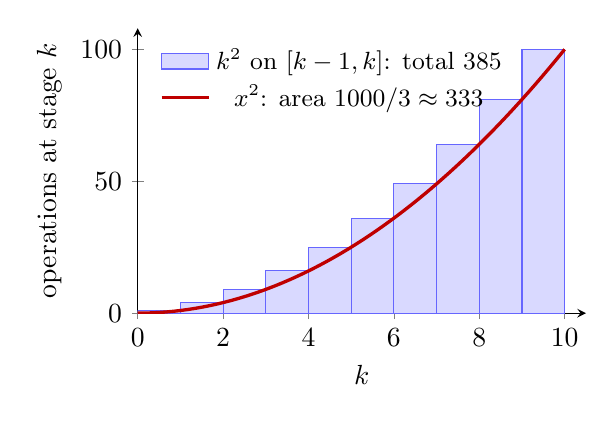
\begin{tikzpicture}
\begin{axis}[width=0.6\textwidth, height=5.2cm, xmin=0, xmax=10.5, ymin=0, ymax=108,
  xlabel={$k$}, ylabel={operations at stage $k$}, xtick={0,2,4,6,8,10},
  axis lines=left, legend pos=north west, legend style={font=\small,draw=none,fill=none}]
  \addplot[ybar interval, area legend, fill=blue!15, draw=blue!60] coordinates
    {(0,1) (1,4) (2,9) (3,16) (4,25) (5,36) (6,49) (7,64) (8,81) (9,100) (10,100)};
  \addlegendentry{$k^2$ on $[k-1,k]$: total $385$}
  \addplot[very thick, red!75!black, domain=0:10, samples=60] {x^2};
  \addlegendentry{$x^2$: area $1000/3\approx333$}
\end{axis}
\end{tikzpicture}
\caption{The work of elimination for $n=10$. Stage $k$ works on a $k\times k$ block and costs
about $k^2$ operations (bars). The bars and the parabola $x^2$ enclose nearly the same area,
so the total is about $\int_0^n x^2\,dx=n^3/3$. The exact count $\frac13(n^3-n)=330$ is even
closer, because the true cost of stage $k$ is $k^2-k$.}\label{fig:u05-cost}
\end{figure}

The cube matters. For $n=100$ elimination costs $\tfrac13(10^6-100)=333{,}300$ operations;
for $n=1000$ about $3.3\times10^8$. Doubling $n$ multiplies the work by $8$. Each additional
right-hand side costs only $n^2$, so a computer factors $A=LU$ once (the expensive part) and
then solves for many vectors $\vb{b}$ cheaply. Matrices with many zeros in good positions
(band matrices, for instance) cost far less, since zero entries need no elimination. By
contrast, the determinant formula with $n!$ terms (Section~\ref{sec:u21}) would be hopeless
for even $n=25$.

\subsection{Row exchanges and permutation matrices}

If a zero appears in a pivot position, elimination needs a row exchange, which is
multiplication by a permutation matrix (Definition~\ref{def:u03-perm}). For $3\times3$
matrices there are exactly six permutation matrices, one for each ordering of the rows of $I$:
\[
  I=\begin{bmatrix} 1&0&0\\ 0&1&0\\ 0&0&1\end{bmatrix},
  P_{12}=\begin{bmatrix} 0&1&0\\ 1&0&0\\ 0&0&1\end{bmatrix},
  P_{13}=\begin{bmatrix} 0&0&1\\ 0&1&0\\ 1&0&0\end{bmatrix},
  P_{23}=\begin{bmatrix} 1&0&0\\ 0&0&1\\ 0&1&0\end{bmatrix},
  \begin{bmatrix} 0&1&0\\ 0&0&1\\ 1&0&0\end{bmatrix},
  \begin{bmatrix} 0&0&1\\ 1&0&0\\ 0&1&0\end{bmatrix}.
\]
The first four leave rows alone or exchange one pair; the last two move all three rows in a
cycle (the fifth sends row~2 up to row~1, row~3 up to row~2 and row~1 down to row~3). The
family is closed: a product of two of them reorders rows twice, which is again a reordering,
and the inverse of each one is also in the list. The exchanges $P_{12},P_{13},P_{23}$ are their
own inverses, and the two cycles are inverses of each other. In every case the inverse is the
transpose, $P^{-1}=P\T$, a fact proved in Section~\ref{sec:u06}. There are $n!$ permutation
matrices of size $n$: $6$ for $n=3$ and $24$ for $n=4$.

With exchanges allowed, $A=LU$ becomes $PA=LU$: put the rows in a good order first, then
eliminate. The smallest example is $A=\begin{bmatrix} 0&2\\ 3&4\end{bmatrix}$. Its first pivot
position holds $0$, so exchange the rows: $P_{12}A=\begin{bmatrix} 3&4\\ 0&2\end{bmatrix}$,
which is already upper triangular, so $L=I$ and $U=P_{12}A$. Section~\ref{sec:u06} completes the
story with a $3\times3$ example.

\subsection{Exercises}

\begin{exercise}\label{ex:u05-EA}
Which matrix $E$ puts $A=\begin{bmatrix} 1&3&0\\ 2&4&0\\ 2&0&1\end{bmatrix}$ into triangular form
$EA=U$? Multiply by $E^{-1}=L$ to factor $A=LU$.
\end{exercise}
\begin{solution}
The multipliers are $\ell_{21}=2$ (row~2 becomes $(0,-2,0)$), $\ell_{31}=2$ (row~3 becomes
$(0,-6,1)$) and $\ell_{32}=-6/-2=3$ (row~3 becomes $(0,0,1)$). So
$U=\begin{bmatrix} 1&3&0\\ 0&-2&0\\ 0&0&1\end{bmatrix}$ and
\[
  E=E_{32}E_{31}E_{21}
  =\begin{bmatrix} 1&0&0\\ 0&1&0\\ 0&-3&1\end{bmatrix}
   \begin{bmatrix} 1&0&0\\ 0&1&0\\ -2&0&1\end{bmatrix}
   \begin{bmatrix} 1&0&0\\ -2&1&0\\ 0&0&1\end{bmatrix}
  =\begin{bmatrix} 1&0&0\\ -2&1&0\\ 4&-3&1\end{bmatrix}.
\]
(The $4$ is $-2-3\cdot(-2)$: row~3 lost $2$ of row~1 directly and gained $6$ of it through row~2.)
The inverse just collects the multipliers:
$L=E^{-1}=\begin{bmatrix} 1&0&0\\ 2&1&0\\ 2&3&1\end{bmatrix}$, and one checks
$LU=\begin{bmatrix} 1&3&0\\ 2&6-2&0\\ 2&6-6&1\end{bmatrix}=A$.
\end{solution}

\begin{exercise}\label{ex:u05-abcd}
Compute $L$ and $U$ for the symmetric matrix
$A=\begin{bmatrix} a&a&a&a\\ a&b&b&b\\ a&b&c&c\\ a&b&c&d\end{bmatrix}$. Find four conditions on
$a,b,c,d$ for $A=LU$ with four pivots.
\end{exercise}
\begin{solution}
Subtract row~1 from rows~2, 3 and~4 (multipliers $1$): the rows become
$(0,b-a,b-a,b-a)$, $(0,b-a,c-a,c-a)$, $(0,b-a,c-a,d-a)$. Subtract the new row~2 from rows~3
and~4 (multipliers $1$): $(0,0,c-b,c-b)$ and $(0,0,c-b,d-b)$. Subtract row~3 from row~4
(multiplier $1$): $(0,0,0,d-c)$. Hence
\[
  L=\begin{bmatrix} 1&0&0&0\\ 1&1&0&0\\ 1&1&1&0\\ 1&1&1&1\end{bmatrix},\qquad
  U=\begin{bmatrix} a&a&a&a\\ 0&b-a&b-a&b-a\\ 0&0&c-b&c-b\\ 0&0&0&d-c\end{bmatrix}.
\]
Four nonzero pivots, with no row exchanges, require $a\neq0$, $b\neq a$, $c\neq b$ and
$d\neq c$.
\end{solution}

\begin{trap}
The posted solution to this problem lists the last condition as $d=c$. That is a slip: with
$d=c$ the fourth pivot $d-c$ is zero. The four conditions are all inequalities.
\end{trap}

\begin{exercise}\label{ex:u05-ab}
Find the $LU$ factorization of $A=\begin{bmatrix} 1&0&1\\ a&a&a\\ b&b&a\end{bmatrix}$ when it
exists. For which real numbers $a,b$ does it exist?
\end{exercise}
\begin{solution}
Step $(2,1)$: $\ell_{21}=a$, row~2 becomes $(0,a,0)$. Step $(3,1)$: $\ell_{31}=b$, row~3
becomes $(0,b,a-b)$. Step $(3,2)$ needs the pivot $a$ to be nonzero; then $\ell_{32}=b/a$ and
row~3 becomes $(0,0,a-b)$. So, for $a\neq0$,
\[
  A=\begin{bmatrix} 1&0&0\\ a&1&0\\ b&b/a&1\end{bmatrix}
    \begin{bmatrix} 1&0&1\\ 0&a&0\\ 0&0&a-b\end{bmatrix}.
\]
If $a=0$, row~2 of the partly reduced matrix is zero while row~3 is $(0,b,-b)$; for $b\neq0$
a row exchange is required, and for $b=0$ there is no pivot in column~2 at all. Either way
there is no $LU$ factorization with a nonzero second pivot, so the condition is $a\neq0$.
The third pivot $a-b$ may be zero: for $a=b\neq0$ the matrix is singular, yet $A=LU$
exists, because no row exchange was needed to reach $U$. Always check by multiplying: row~3
of $LU$ is $b(1,0,1)+\tfrac ba(0,a,0)+(0,0,a-b)=(b,b,a)$.
\end{solution}

\begin{exercise}\label{ex:u05-time}
A computer performs $10^9$ operations per second. Using Proposition~\ref{prop:u05-count},
estimate the time to factor a full $1000\times1000$ matrix, the time for each additional
right-hand side, and the time to factor a $10{,}000\times10{,}000$ matrix.
\end{exercise}
\begin{solution}
For $n=1000$: $\tfrac13(10^9-10^3)\approx3.3\times10^8$ operations, about $0.33$ seconds.
Each right-hand side then costs $n^2=10^6$ operations, one millisecond. For $n=10^4$ the
factorization costs about $\tfrac13\times10^{12}$ operations, roughly $333$ seconds or five
and a half minutes: ten times the size, a thousand times the work. (Real machines are faster,
and sparse matrices are much cheaper, but the $n^3$ growth is the same.)
\end{solution}

% unit: u06
% sources: sources/067-transposes-permutations-vector-spaces.txt, sources/137-transposes-permutations-vector-spaces.txt, sources/138-mit18-06scf11-ses1-5sum-pdf-download-file.txt, sources/139-subspaces-of-three-dimensional-space.txt, sources/140-mit18-06scf11-ses1-5prob-pdf-download-file.txt, sources/141-mit18-06scf11-ses1-5sol-pdf-download-file.txt
\section{Transposes, permutations, vector spaces}\label{sec:u06}

This section closes the chapter on elimination and opens the one on vector spaces. First we
finish two loose ends: permutation matrices, which complete $A=LU$ to $PA=LU$, and
transposes, which produce the symmetric matrices that dominate applications. Then comes
the step that turns a toolbox of computations into linear algebra proper: instead of
individual vectors we study \emph{spaces} of vectors, and especially the subspaces that live
inside $\R^n$. The first such subspace attached to a matrix is its column space.

\subsection{Permutations complete elimination: \texorpdfstring{\(PA=LU\)}{PA = LU}}

A permutation matrix is the identity with its rows reordered
(Definition~\ref{def:u03-perm}); $PA$ puts the rows of $A$ in the same new order. There is
one permutation matrix for each ordering of $n$ rows. The first row of $P$ can be any of the
$n$ rows of $I$, the second any of the remaining $n-1$, and so on, so there are
$n(n-1)\cdots2\cdot1=n!$ permutation matrices of size $n$: $6$ when $n=3$, $24$ when $n=4$,
$120$ when $n=5$.

\begin{theorem}[The inverse of a permutation is its transpose]\label{thm:u06-PTP}
Every permutation matrix satisfies $P\T P=I$, so $P^{-1}=P\T$.
\end{theorem}

\begin{proof}
The rows of $P$ are the rows of $I$ in a new order, so each column of $P$ contains exactly
one $1$ and the columns of $P$ are the standard vectors $\vb{e}_1,\dots,\vb{e}_n$ in some
order, each appearing once. The $(i,j)$ entry of $P\T P$ is (column $i$ of $P$)$\cdot$(column $j$
of $P$). For $i=j$ this is $\vb{e}_k\cdot\vb{e}_k=1$; for $i\neq j$ it is the dot product of two
different standard vectors, which is $0$. Hence $P\T P=I$, and by
Corollary~\ref{cor:u04-onesided} $P\T$ is the inverse of $P$.
\end{proof}

Section~\ref{sec:u05} factored $A=LU$ when elimination needs no row exchanges. Most matrices
need none, but some do: a zero can land in a pivot position while a nonzero sits below it.
The cure is to do all the necessary exchanges first.

\begin{theorem}[$PA=LU$]\label{thm:u06-PALU}
If $A$ is an invertible $n\times n$ matrix, there is a permutation matrix $P$ such that
elimination on $PA$ needs no row exchanges, so that $PA=LU$ with $L$ lower triangular with
unit diagonal and $U$ upper triangular with the (nonzero) pivots on its diagonal.
\end{theorem}

\begin{proof}[Sketch]
Run elimination on $A$, exchanging rows whenever a pivot position holds zero; since $A$ is
invertible a nonzero entry is always available below (Theorem~\ref{thm:u04-test}). Let $P$
be the product of all the exchanges made. A row exchange only swaps two rows that are not yet
pivot rows, and elimination never mixes a row into the rows above it, so performing all the
exchanges at the very start puts every row where it eventually ends up. Elimination on $PA$
then meets the same pivots in the same places and needs no exchange, and
Theorem~\ref{thm:u05-LU} gives $PA=LU$. (In the bookkeeping, a later exchange of rows $i$ and
$k$ also exchanges the multipliers already recorded in those rows of $L$.)
\end{proof}

\begin{example}[A $3\times3$ factorization $PA=LU$]\label{ex:u06-PALU}
Let $A=\begin{bmatrix} 0&2&1\\ 1&1&1\\ 2&0&3\end{bmatrix}$. The $(1,1)$ position holds $0$,
so exchange rows~1 and~2:
\[
  P_{12}A=\begin{bmatrix} 1&1&1\\ 0&2&1\\ 2&0&3\end{bmatrix}.
\]
Now eliminate without further exchanges: $\ell_{21}=0$; $\ell_{31}=2$ turns row~3 into
$(2,0,3)-2(1,1,1)=(0,-2,1)$; then $\ell_{32}=-2/2=-1$ turns it into
$(0,-2,1)+(0,2,1)=(0,0,2)$. Therefore
\[
  \underbrace{\begin{bmatrix} 0&1&0\\ 1&0&0\\ 0&0&1\end{bmatrix}}_{P}
  \underbrace{\begin{bmatrix} 0&2&1\\ 1&1&1\\ 2&0&3\end{bmatrix}}_{A}
  =\underbrace{\begin{bmatrix} 1&0&0\\ 0&1&0\\ 2&-1&1\end{bmatrix}}_{L}
  \underbrace{\begin{bmatrix} 1&1&1\\ 0&2&1\\ 0&0&2\end{bmatrix}}_{U}.
\]
Check row~3: $2\,(1,1,1)-1\,(0,2,1)+1\,(0,0,2)=(2,0,3)$, which is row~3 of $PA$. The pivots
are $1,2,2$, and $A$ itself has no $LU$ factorization because its first pivot position holds
zero.
\end{example}

In practice, software exchanges rows more often than algebra requires. MATLAB's elimination
chooses, in each column, the largest available entry as the pivot (\emph{partial pivoting}):
dividing by a tiny pivot would magnify rounding errors. The algebra is the same, $PA=LU$;
only $P$ changes.

\subsection{Transposes and symmetric matrices}

The transpose (Definition~\ref{def:u05-transpose}) flips a matrix across its main diagonal,
$(A\T)_{ij}=a_{ji}$; the rows of $A$ become the columns of $A\T$. A $3\times2$ matrix becomes
$2\times3$:
\[
  \begin{bmatrix} 1&3\\ 2&3\\ 4&1\end{bmatrix}\T=\begin{bmatrix} 1&2&4\\ 3&3&1\end{bmatrix}.
\]

\begin{definition}[Symmetric matrix]\label{def:u06-symmetric}
A square matrix $S$ is \emph{symmetric} if $S\T=S$, that is, $s_{ij}=s_{ji}$ for all $i,j$.
\end{definition}

The diagonal of a symmetric matrix is unrestricted, and each entry above the diagonal is
mirrored below it, as in
$\begin{bmatrix} 3&1&7\\ 1&2&9\\ 7&9&4\end{bmatrix}$. Symmetric matrices are the most
important special family in applications, and the most common way they arise is this.

\begin{theorem}[$R\T R$ is symmetric]\label{thm:u06-RTR}
For every $m\times n$ matrix $R$, the $n\times n$ matrix $R\T R$ is symmetric, and so is the
$m\times m$ matrix $RR\T$.
\end{theorem}

\begin{proof}
By the rule for transposes of products (Theorem~\ref{thm:u05-transpose-product}) and
$(R\T)\T=R$,
\[
  (R\T R)\T=R\T(R\T)\T=R\T R .
\]
The same computation with $R\T$ in place of $R$ shows $(RR\T)\T=RR\T$.
\end{proof}

\begin{example}[Building symmetric matrices from a rectangular one]\label{ex:u06-RTR}
Take the $2\times3$ matrix $R=\begin{bmatrix} 1&2&4\\ 3&3&1\end{bmatrix}$. Then
\[
  R\T R=\begin{bmatrix} 1&3\\ 2&3\\ 4&1\end{bmatrix}\begin{bmatrix} 1&2&4\\ 3&3&1\end{bmatrix}
  =\begin{bmatrix} 10&11&7\\ 11&13&11\\ 7&11&17\end{bmatrix},\qquad
  RR\T=\begin{bmatrix} 21&13\\ 13&19\end{bmatrix}.
\]
The $(1,2)$ entry of $R\T R$ is row~1 of $R\T$ times column~2 of $R$, namely
$(1,3)\cdot(2,3)=11$; the $(2,1)$ entry is $(2,3)\cdot(1,3)$, the same dot product taken in
the other order. In general $(R\T R)_{ij}$ is the dot product of columns $i$ and $j$ of $R$,
which is why the matrix must be symmetric. The product $R\T R$ will be central to least
squares (Section~\ref{sec:u17}).
\end{example}

\subsection{Vector spaces}

The two operations we perform on vectors are adding them and multiplying them by
numbers (scalars). A \emph{space} of vectors is a collection in which these operations can
always be carried out without leaving the collection.

\begin{definition}[The space \texorpdfstring{$\R^n$}{Rn}]\label{def:u06-Rn}
$\R^n$ is the set of all column vectors with $n$ real components, with addition and scalar
multiplication done component by component.
\end{definition}

$\R^2$ contains $(3,2)$, $(0,0)$, $(\pi,e)$ and every other pair of real numbers; drawn as
arrows from the origin (or as their endpoints), it is the whole $xy$-plane. The vector
$(3,2,0)$ belongs to $\R^3$, not to $\R^2$: it has three components, one of which happens to
be zero.

\begin{definition}[Vector space]\label{def:u06-vspace}
A \emph{vector space} is a nonempty set $V$ of objects (vectors) with an addition and a
multiplication by real scalars such that $V$ is \emph{closed} under both: if $\vb{v},\vb{w}\in V$
and $c\in\R$, then $\vb{v}+\vb{w}\in V$ and $c\vb{v}\in V$. The operations must obey the usual
rules: $\vb{v}+\vb{w}=\vb{w}+\vb{v}$; $(\vb{u}+\vb{v})+\vb{w}=\vb{u}+(\vb{v}+\vb{w})$; there is a
zero vector with $\vb{v}+\vb{0}=\vb{v}$; each $\vb{v}$ has a negative with $\vb{v}+(-\vb{v})=\vb{0}$;
$1\vb{v}=\vb{v}$; $c(d\vb{v})=(cd)\vb{v}$; $c(\vb{v}+\vb{w})=c\vb{v}+c\vb{w}$; and
$(c+d)\vb{v}=c\vb{v}+d\vb{v}$.
\end{definition}

In $\R^n$ the eight rules hold automatically, because they hold for each component; the
question in practice is always closure. Closure under both operations is the same as closure
under linear combinations $c\vb{v}+d\vb{w}$. Vector spaces need not consist of columns:
the set of all $2\times2$ matrices, with the usual addition and scalar multiplication, is a
vector space too (Section~\ref{sec:u12} studies such spaces).

\begin{proposition}[Every vector space contains zero]\label{prop:u06-zero}
If $V$ is a vector space, then $\vb{0}\in V$.
\end{proposition}

\begin{proof}
$V$ is nonempty; pick any $\vb{v}\in V$. Closure under scalar multiplication puts
$0\cdot\vb{v}$ in $V$, and $0\cdot\vb{v}=(0+0)\vb{v}=0\cdot\vb{v}+0\cdot\vb{v}$; adding the
negative of $0\cdot\vb{v}$ to both sides gives $0\cdot\vb{v}=\vb{0}$.
\end{proof}

So the $xy$-plane with the origin removed is not a vector space. Neither is the quarter-plane
$Q$ of vectors with both components nonnegative: adding two vectors of $Q$ stays in $Q$, but
$-1\cdot(3,2)=(-3,-2)$ does not. $Q$ is closed under addition but not under multiplication by
all real numbers (right panel of Figure~\ref{fig:u06-subspaces}).

\subsection{Subspaces}

\begin{definition}[Subspace]\label{def:u06-subspace}
A \emph{subspace} of a vector space $V$ is a nonempty subset $S\subseteq V$ that is itself a
vector space with the same operations. Equivalently, $S$ is nonempty and closed under
addition and scalar multiplication: $\vb{v},\vb{w}\in S$ and $c\in\R$ imply
$\vb{v}+\vb{w}\in S$ and $c\vb{v}\in S$.
\end{definition}

The two descriptions agree because the eight rules are inherited from $V$, and the zero
vector and negatives lie in $S$ by closure ($0\vb{v}=\vb{0}$, $(-1)\vb{v}=-\vb{v}$). By
Proposition~\ref{prop:u06-zero} every subspace contains $\vb{0}$.

If a subspace of $\R^2$ contains a nonzero vector $\vb{v}$, it contains every multiple
$c\vb{v}$: the whole line through $\vb{0}$ and $\vb{v}$. That line $L=\{c\vb{v}:c\in\R\}$ is a
subspace, since $c\vb{v}+d\vb{v}=(c+d)\vb{v}$ and $k(c\vb{v})=(kc)\vb{v}$ stay on it. A line that
misses the origin is never a subspace: multiplying one of its vectors by $0$ leaves the line
(left panel of Figure~\ref{fig:u06-subspaces}).

\begin{figure}[ht]
\centering
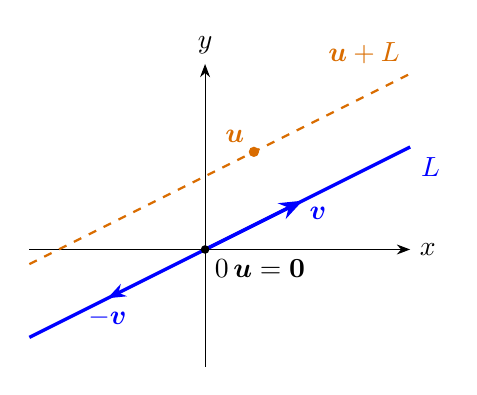
\begin{tikzpicture}[scale=0.62,>=Stealth]
  \draw[->] (-3.6,0) -- (4.2,0) node[right] {$x$};
  \draw[->] (0,-2.4) -- (0,3.8) node[above] {$y$};
  \draw[very thick,blue] (-3.6,-1.8) -- (4.2,2.1) node[below right] {$L$};
  \draw[thick,dashed,orange!85!black] (-3.6,-0.3) -- (4.2,3.6) node[above left] {$\vb{u}+L$};
  \draw[->,very thick,blue] (0,0) -- (2,1) node[below right=-2pt] {$\vb{v}$};
  \draw[->,thick,blue] (0,0) -- (-2,-1) node[below] {$-\vb{v}$};
  \fill[orange!85!black] (1,2) circle (3pt) node[above left] {$\vb{u}$};
  \fill (0,0) circle (2.5pt) node[below right] {$0\,\vb{u}=\vb{0}$};
\end{tikzpicture}
\qquad
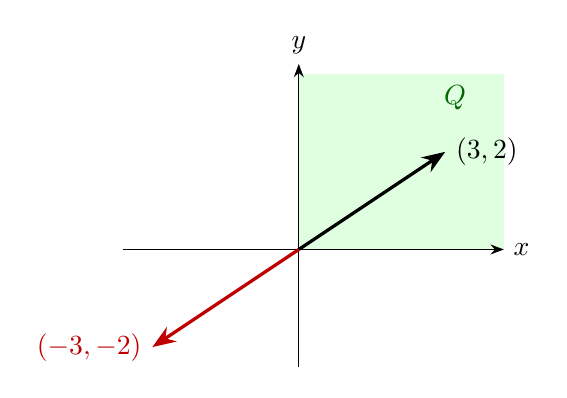
\begin{tikzpicture}[scale=0.62,>=Stealth]
  \fill[green!12] (0,0) rectangle (4.2,3.6);
  \draw[->] (-3.6,0) -- (4.2,0) node[right] {$x$};
  \draw[->] (0,-2.4) -- (0,3.8) node[above] {$y$};
  \node[green!40!black] at (3.2,3.1) {$Q$};
  \draw[->,very thick] (0,0) -- (3,2) node[right] {$(3,2)$};
  \draw[->,very thick,red!75!black] (0,0) -- (-3,-2) node[left] {$(-3,-2)$};
\end{tikzpicture}
\caption{Left: the line $L$ through the origin (all multiples of $\vb{v}$) is a subspace of
$\R^2$. The parallel dashed line through $\vb{u}=(1,2)$ is not: $0\,\vb{u}=\vb{0}$ is not on it.
Right: the quarter-plane $Q$ is closed under addition but not under scalar multiplication,
since $-1\cdot(3,2)$ leaves it.}\label{fig:u06-subspaces}
\end{figure}

\begin{proposition}[The subspaces of \texorpdfstring{$\R^2$}{R2}]\label{prop:u06-R2}
Every subspace of $\R^2$ is one of: the zero subspace $Z=\{\vb{0}\}$; a line through the
origin; all of $\R^2$.
\end{proposition}

\begin{proof}
Let $S$ be a subspace. If $S=\{\vb{0}\}$ we are done. Otherwise $S$ contains some
$\vb{v}\neq\vb{0}$ and hence the line $L$ of its multiples. If $S=L$ we are done. Otherwise $S$
contains a vector $\vb{w}$ off that line, so $\delta=v_1w_2-v_2w_1\neq0$ (if $\delta=0$, $\vb{w}$
would be a multiple of $\vb{v}$). For any $\vb{b}\in\R^2$, the weights
$x=(b_1w_2-b_2w_1)/\delta$ and $y=(v_1b_2-v_2b_1)/\delta$ satisfy $x\vb{v}+y\vb{w}=\vb{b}$, as
direct substitution confirms. By closure $\vb{b}\in S$, so $S=\R^2$.
\end{proof}

Similarly, the subspaces of $\R^3$ are $Z$, the lines through the origin, the planes through
the origin, and $\R^3$ itself; the proof uses the idea of dimension
(Section~\ref{sec:u10}). A line through the origin in $\R^2$ looks like $\R^1$, but it is not
$\R^1$: its vectors have two components.

\begin{trap}
$\R^2$ is \emph{not} a subspace of $\R^3$: its vectors have two components, so it is not
even a subset of $\R^3$. The plane of vectors $(x,y,0)$ \emph{is} a subspace of $\R^3$; it
looks like $\R^2$ but is a different set. Also, closure under addition alone proves
nothing (the quarter-plane passes that test); always check scalar multiplication by negative
numbers and by zero.
\end{trap}

\subsection{The column space of a matrix}

Subspaces of $\R^m$ come naturally from matrices. Put two vectors in the columns of a matrix;
a subspace containing them must contain all their combinations, and the set of all
combinations is already a subspace.

\begin{definition}[Column space]\label{def:u06-colspace}
The \emph{column space} $\Col{A}$ of an $m\times n$ matrix $A$ is the set of all linear
combinations of the columns of $A$. Equivalently, $\Col{A}=\{A\vb{x}:\vb{x}\in\R^n\}$. It is a
subspace of $\R^m$.
\end{definition}

It is a subspace because $A\vb{x}+A\vb{y}=A(\vb{x}+\vb{y})$ and $c(A\vb{x})=A(c\vb{x})$ are again
of the form $A(\text{something})$.

\begin{example}[A plane in \texorpdfstring{$\R^3$}{R3}]\label{ex:u06-colspace}
Let $A=\begin{bmatrix} 1&3\\ 2&3\\ 4&1\end{bmatrix}$. Its columns $(1,2,4)$ and $(3,3,1)$ are
vectors in $\R^3$ that do not lie on one line, so their combinations fill a plane through the
origin: $\Col{A}$ is a plane in $\R^3$. It contains $\vb{0}$, both columns, their sum
$(4,5,5)$, and, e.g., $(1,2,4)+3(3,3,1)=(10,11,7)$. Which plane? A vector $\vb{b}$ is in
$\Col{A}$ when $x_1(1,2,4)+x_2(3,3,1)=\vb{b}$ can be solved. Eliminate on the augmented matrix:
\[
  \left[\begin{array}{rr|l} 1&3&b_1\\ 2&3&b_2\\ 4&1&b_3\end{array}\right]
  \to
  \left[\begin{array}{rr|l} 1&3&b_1\\ 0&-3&b_2-2b_1\\ 0&-11&b_3-4b_1\end{array}\right]
  \to
  \left[\begin{array}{rr|l} 1&3&b_1\\ 0&-3&b_2-2b_1\\ 0&0&b_3-4b_1-\tfrac{11}{3}(b_2-2b_1)\end{array}\right].
\]
The last row says $0=\tfrac{10}{3}b_1-\tfrac{11}{3}b_2+b_3$. So
\[
  \Col{A}=\{\vb{b}\in\R^3: 10b_1-11b_2+3b_3=0\}.
\]
Check: $(1,2,4)$ gives $10-22+12=0$, $(3,3,1)$ gives $30-33+3=0$, $(4,5,5)$ gives
$40-55+15=0$. The vector $(1,0,0)$ gives $10\neq0$; it is not in the column space, and
$A\vb{x}=(1,0,0)$ has no solution.
\end{example}

The same construction works in any dimension: five vectors in $\R^{10}$, each with ten
components, have combinations that fill a subspace of $\R^{10}$, at most five-dimensional and
smaller if the vectors are dependent. How the column space decides which systems
$A\vb{x}=\vb{b}$ are solvable is the subject of Section~\ref{sec:u07}.

\subsection{Exercises}

\begin{exercise}\label{ex:u06-cycle}
(a) Find a $3\times3$ permutation matrix with $P^3=I$ but $P\neq I$. (b) Find a $4\times4$
permutation matrix $\widehat{P}$ with $\widehat{P}^4\neq I$.
\end{exercise}
\begin{solution}
(a) Move the rows in a cycle: row~1 to position~2, row~2 to position~3, row~3 to position~1.
\[
  P=\begin{bmatrix} 0&0&1\\ 1&0&0\\ 0&1&0\end{bmatrix},\qquad
  P^2=\begin{bmatrix} 0&1&0\\ 0&0&1\\ 1&0&0\end{bmatrix},\qquad P^3=I .
\]
Indeed $P(1,2,3)=(3,1,2)$, and applying the cycle three times returns every row home.
(b) Use the block matrix $\widehat{P}=\begin{bmatrix} 1&0\\ 0&P\end{bmatrix}$, which leaves
row~1 alone and cycles rows~2, 3, 4. By block multiplication $\widehat{P}^3=I$, so
$\widehat{P}^4=\widehat{P}\neq I$.
\end{solution}

\begin{exercise}\label{ex:u06-count}
How many entries of a $4\times4$ matrix $A$ can be chosen independently if (a) $A$ is
symmetric; (b) $A$ is skew-symmetric, $A\T=-A$?
\end{exercise}
\begin{solution}
(a) The $4$ diagonal entries and the $6$ entries above the diagonal are free; the $6$ below
are copies. So $10$ entries:
$A=\begin{bmatrix} a&e&f&g\\ e&b&h&i\\ f&h&c&j\\ g&i&j&d\end{bmatrix}$.
(b) Now $a_{ii}=-a_{ii}$ forces a zero diagonal, and the entries below the diagonal are the
negatives of those above. So $6$ entries:
$A=\begin{bmatrix} 0&-a&-b&-c\\ a&0&-d&-e\\ b&d&0&-f\\ c&e&f&0\end{bmatrix}$.
\end{solution}

\begin{exercise}\label{ex:u06-matrix-subspaces}
In the vector space $M$ of all $n\times n$ matrices, decide which of these are subspaces:
(a) the symmetric matrices; (b) the skew-symmetric matrices; (c) the unsymmetric matrices
($A\T\neq A$).
\end{exercise}
\begin{solution}
(a) Yes. If $A\T=A$ and $B\T=B$, then $(A+B)\T=A\T+B\T=A+B$ and $(cA)\T=cA\T=cA$.
(b) Yes. If $A\T=-A$ and $B\T=-B$, then $(A+B)\T=-A-B=-(A+B)$ and $(cA)\T=-cA$.
(c) No. The zero matrix is symmetric, so it is not in the set; and the set is not closed
under addition:
$\begin{bmatrix} 1&1\\ 0&0\end{bmatrix}+\begin{bmatrix} 0&0\\ 1&1\end{bmatrix}
=\begin{bmatrix} 1&1\\ 1&1\end{bmatrix}$, two unsymmetric matrices with a symmetric sum.
\end{solution}

\begin{exercise}\label{ex:u06-lines}
Let $\vb{x}_1=(1,2,3)$ and $\vb{x}_2=(1,3,0)$ in $\R^3$. Let $V_1$ and $V_2$ be the smallest
subspaces containing $\vb{x}_1$, respectively $\vb{x}_2$, and $V_3$ the smallest subspace
containing both. (a) Describe $V_1$, $V_2$ and $V_1\cap V_2$. (b) Is $V_1\cup V_2$ a subspace? Is it
$V_3$? (c) Find a subspace $S$ of $V_3$ containing neither $\vb{x}_1$ nor $\vb{x}_2$.
(d) Describe $V_3\cap\{\text{the $xy$-plane}\}$.
\end{exercise}
\begin{solution}
(a) A subspace containing $\vb{x}_1$ contains all its multiples, and the multiples already form
a subspace, so $V_1$ is the line through $(1,2,3)$; likewise $V_2$ is the line through
$(1,3,0)$. If $c(1,2,3)=d(1,3,0)$, the third components give $3c=0$, so $c=0=d$: the lines meet
only at the origin, and $V_1\cap V_2=\{\vb{0}\}$, the zero subspace.
(b) No. $\vb{x}_1+\vb{x}_2=(2,5,3)$ is on neither line ($(2,5,3)$ is not a multiple of $(1,2,3)$
since $5\neq2\cdot2$, and its third component is not $0$), so the union is not closed under
addition and cannot equal $V_3$. Instead $V_3$ is the plane of all combinations
$s\vb{x}_1+t\vb{x}_2=(s+t,\,2s+3t,\,3s)$. Eliminating $s=b_3/3$ and $t=b_1-b_3/3$ from
$b_2=2s+3t$ gives its equation $9b_1-3b_2-b_3=0$.
(c) The line through $\vb{x}_1+\vb{x}_2=(2,5,3)$ lies in $V_3$ and contains neither
$\vb{x}_1$ nor $\vb{x}_2$ (neither is a multiple of $(2,5,3)$). Other choices, such as the line
through $2\vb{x}_1+\vb{x}_2$, work too.
(d) Points of the $xy$-plane have $b_3=0$; on $V_3$ this forces $9b_1=3b_2$, i.e.\ $b_2=3b_1$.
So the intersection is the line through $(1,3,0)$, which is $V_2$. This makes sense: $\vb{x}_2$
lies in both planes, and two different planes through the origin meet in a line.
\end{solution}

% unit: u07
% sources: sources/090-column-space-and-nullspace.txt, sources/142-column-space-and-nullspace.txt, sources/143-mit18-06scf11-ses1-6sum-pdf-download-file.txt, sources/144-vector-subspaces.txt, sources/145-mit18-06scf11-ses1-6prob-pdf-download-file.txt, sources/146-mit18-06scf11-ses1-6sol-pdf-download-file.txt, short_plan.json (s02)
\section{Column space and nullspace}\label{sec:u07}

Every matrix carries two subspaces that answer the two basic questions about
$A\vb{x}=\vb{b}$. The \emph{column space} $\Col{A}$ answers ``for which $\vb{b}$ is there a
solution?'': exactly those $\vb{b}$ that are combinations of the columns. The
\emph{nullspace} $\Nul{A}$ answers ``how many solutions are there?'': any two solutions differ
by a vector that $A$ sends to zero. The two subspaces are built in opposite ways. The column
space is \emph{spanned}: we are handed some vectors and take all their combinations. The
nullspace is \emph{cut out by equations}: we are told the conditions $A\vb{x}=\vb{0}$ and must
find which vectors satisfy them. This section works both out for small examples by inspection;
Section~\ref{sec:u08} gives the systematic method by elimination.

\subsection{Unions and intersections of subspaces}

Recall that a subspace is a nonempty set of vectors closed under addition and scalar
multiplication (Definition~\ref{def:u06-subspace}); equivalently, for any $\vb{v},\vb{w}$ in
the subspace and any numbers $c,d$, the combination $c\vb{v}+d\vb{w}$ is in it. In $\R^3$ a plane
$P$ through the origin and a line $L$ through the origin are subspaces. What about combining
them?

\emph{The union is usually not a subspace.} Take $P$ to be the $x_1x_2$-plane (vectors
$(x_1,x_2,0)$) and $L$ the $x_3$-axis. Then $(1,0,0)\in P$ and $(0,0,1)\in L$, but their sum
$(1,0,1)$ is in neither, so $P\cup L$ is not closed under addition.

\begin{theorem}[Intersections of subspaces are subspaces]\label{thm:u07-intersection}
If $S$ and $T$ are subspaces of a vector space $V$, then $S\cap T$, the set of vectors lying
in both, is a subspace of $V$.
\end{theorem}

\begin{proof}
$\vb{0}$ lies in both $S$ and $T$ (Proposition~\ref{prop:u06-zero}), so $S\cap T$ is nonempty.
Let $\vb{v},\vb{w}\in S\cap T$ and $c,d\in\R$. Since $\vb{v},\vb{w}\in S$ and $S$ is a subspace,
$c\vb{v}+d\vb{w}\in S$. Since $\vb{v},\vb{w}\in T$ and $T$ is a subspace, $c\vb{v}+d\vb{w}\in T$.
So $c\vb{v}+d\vb{w}\in S\cap T$.
\end{proof}

For the plane and line above, $P\cap L=\{\vb{0}\}$, the zero subspace. Intersecting adds
requirements, so the intersection is usually smaller, but it is always a subspace.
(Exercise~\ref{ex:u07-sum} shows that the right way to combine two subspaces into a bigger
one is their sum $S+T$, not their union.)

\subsection{The column space decides solvability}

Our example is the $4\times3$ matrix
\begin{equation}\label{eq:u07-A}
  A=\begin{bmatrix} 1&1&2\\ 2&1&3\\ 3&1&4\\ 4&1&5\end{bmatrix},\qquad
  A\vb{x}=x_1\begin{bmatrix}1\\2\\3\\4\end{bmatrix}+x_2\begin{bmatrix}1\\1\\1\\1\end{bmatrix}
         +x_3\begin{bmatrix}2\\3\\4\\5\end{bmatrix}=\begin{bmatrix}b_1\\b_2\\b_3\\b_4\end{bmatrix}.
\end{equation}
Its columns are vectors in $\R^4$, so its column space
$\Col{A}=\{A\vb{x}:\vb{x}\in\R^3\}$ (Definition~\ref{def:u06-colspace}) is a subspace of
$\R^4$. These are four equations in only three unknowns, and we should not expect a solution
for every $\vb{b}$: the combinations of three vectors cannot fill four-dimensional space.
But some right-hand sides are fine, and they are exactly the vectors in the column space.

\begin{theorem}[Solvability]\label{thm:u07-solvable}
$A\vb{x}=\vb{b}$ has a solution if and only if $\vb{b}$ is in the column space $\Col{A}$.
\end{theorem}

\begin{proof}
$A\vb{x}$ is the combination of the columns with weights $x_1,\dots,x_n$. If a solution
$\vb{x}$ exists, $\vb{b}=A\vb{x}$ is such a combination, so $\vb{b}\in\Col{A}$. Conversely,
if $\vb{b}$ is a combination $x_1\vb{a}_1+\cdots+x_n\vb{a}_n$, those weights form a solution
$\vb{x}$.
\end{proof}

A good way to find vectors in $\Col{A}$ is to choose $\vb{x}$ first and compute $\vb{b}$. The
right side $\vb{b}=\vb{0}$ is always reached (by $\vb{x}=\vb{0}$); $\vb{b}=(1,2,3,4)$ is
column~1, reached by $\vb{x}=(1,0,0)$; $\vb{b}=(1,1,1,1)$ is column~2, reached by
$\vb{x}=(0,1,0)$.

How big is $\Col{A}$? Column~3 is the sum of columns~1 and~2, so it contributes nothing new:
by Proposition~\ref{prop:u01-dependent} every combination of all three columns is already a
combination of the first two. Columns~1 and~2 are not on one line, so their combinations form
a plane. Hence \emph{$\Col{A}$ is a two-dimensional subspace (a plane) of $\R^4$}. We could
equally have thrown away column~1, since column~1 $=$ column~3 $-$ column~2; the convention
(made precise in Section~\ref{sec:u08}) is to keep the earliest columns that are not
combinations of earlier ones, the \emph{pivot columns}.

\begin{example}[Equations for the column space]\label{ex:u07-colspace}
Which $\vb{b}\in\R^4$ lie in $\Col{A}$? We need $\vb{b}=x_1(1,2,3,4)+x_2(1,1,1,1)$, that is,
$b_i=i\,x_1+x_2$ for $i=1,2,3,4$: the components of $\vb{b}$ must form an arithmetic
progression. That is two equations:
\[
  \Col{A}=\{\vb{b}\in\R^4:\ b_1-2b_2+b_3=0\ \text{and}\ b_2-2b_3+b_4=0\}.
\]
Indeed each column passes both tests (for column~3: $2-6+4=0$ and $3-8+5=0$), and the tests are
preserved by combinations. Conversely, if $\vb{b}$ passes both tests then the differences
$b_2-b_1=b_3-b_2=b_4-b_3$ share a common value $d$, and
$\vb{b}=d\,(1,2,3,4)+(b_1-d)\,(1,1,1,1)$. So $A\vb{x}=(2,3,4,5)$ is solvable (it is column~3),
while $A\vb{x}=(1,2,3,5)$ is not, because $b_2-2b_3+b_4=2-6+5=1\neq0$.
\end{example}

\subsection{The nullspace}

\begin{definition}[Nullspace]\label{def:u07-nullspace}
The \emph{nullspace} of an $m\times n$ matrix $A$ is the set of all solutions of
$A\vb{x}=\vb{0}$:
\[
  \Nul{A}=\{\vb{x}\in\R^n:\ A\vb{x}=\vb{0}\}.
\]
\end{definition}

The column space contains right-hand sides $\vb{b}\in\R^m$; the nullspace contains inputs
$\vb{x}\in\R^n$. For the $4\times3$ example, $\Col{A}\subseteq\R^4$ while
$\Nul{A}\subseteq\R^3$.

\begin{theorem}[The nullspace is a subspace]\label{thm:u07-nullspace}
For every $m\times n$ matrix $A$, $\Nul{A}$ is a subspace of $\R^n$.
\end{theorem}

\begin{proof}
$A\vb{0}=\vb{0}$, so $\vb{0}\in\Nul{A}$. If $A\vb{v}=\vb{0}$ and $A\vb{w}=\vb{0}$, then by the
distributive law $A(\vb{v}+\vb{w})=A\vb{v}+A\vb{w}=\vb{0}+\vb{0}=\vb{0}$, and for any scalar
$c$, $A(c\vb{v})=c\,A\vb{v}=c\,\vb{0}=\vb{0}$. So $\Nul{A}$ is closed under addition and scalar
multiplication.
\end{proof}

\begin{example}[A nullspace that is a line]\label{ex:u07-nullspace}
For $A$ in \eqref{eq:u07-A}, the relation column~1 $+$ column~2 $-$ column~3 $=\vb{0}$ says
that $(1,1,-1)\in\Nul{A}$, and so is every multiple $c(1,1,-1)$. Are there other solutions?
Write $\vb{a}_1,\vb{a}_2$ for the first two columns. Since $\vb{a}_3=\vb{a}_1+\vb{a}_2$,
\[
  A\vb{x}=x_1\vb{a}_1+x_2\vb{a}_2+x_3(\vb{a}_1+\vb{a}_2)=(x_1+x_3)\,\vb{a}_1+(x_2+x_3)\,\vb{a}_2 .
\]
Because $\vb{a}_1$ and $\vb{a}_2$ are not parallel, this combination is zero only when both
weights are zero: $x_1=-x_3$ and $x_2=-x_3$. So $\vb{x}=-x_3(1,1,-1)$, and
\[
  \Nul{A}=\{c\,(1,1,-1):c\in\R\},
\]
a line through the origin in $\R^3$.
\end{example}

\subsection{The solutions of \texorpdfstring{\(A\vb{x}=\vb{b}\)}{Ax = b} are a shifted nullspace}

Now take a right-hand side that is not zero, say $\vb{b}=(1,2,3,4)$. One solution is
$\vb{x}=(1,0,0)$; another is $(0,-1,1)$, since $-$column~2 $+$ column~3 $=(1,2,3,4)$. The
solutions do \emph{not} form a subspace: $\vb{x}=\vb{0}$ is not a solution, because
$A\vb{0}=\vb{0}\neq\vb{b}$. Their structure is described next.

\begin{proposition}[All solutions]\label{prop:u07-allsolutions}
Suppose $A\vb{x}_p=\vb{b}$. Then the solutions of $A\vb{x}=\vb{b}$ are exactly the vectors
$\vb{x}=\vb{x}_p+\vb{x}_n$ with $\vb{x}_n\in\Nul{A}$.
\end{proposition}

\begin{proof}
If $\vb{x}_n\in\Nul{A}$, then $A(\vb{x}_p+\vb{x}_n)=\vb{b}+\vb{0}=\vb{b}$. Conversely, if
$A\vb{x}=\vb{b}$, then $A(\vb{x}-\vb{x}_p)=\vb{b}-\vb{b}=\vb{0}$, so $\vb{x}_n=\vb{x}-\vb{x}_p$
is in $\Nul{A}$ and $\vb{x}=\vb{x}_p+\vb{x}_n$.
\end{proof}

For our example the solutions of $A\vb{x}=(1,2,3,4)$ are $(1,0,0)+c(1,1,-1)$: a line parallel
to the nullspace but shifted away from the origin (Figure~\ref{fig:u07-shifted}); $c=-1$ gives
$(0,-1,1)$. Section~\ref{sec:u09} builds on this to find the complete solution of any system.

\begin{figure}[ht]
\centering
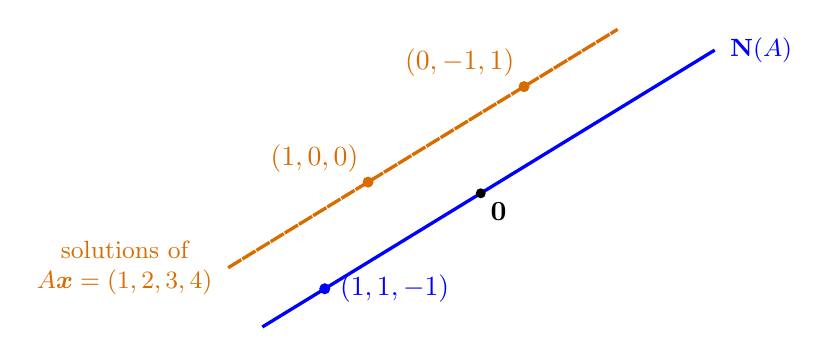
\begin{tikzpicture}
\begin{axis}[view={200}{25}, width=9cm, height=7cm, axis lines=none,
  xmin=-1.6, xmax=2.2, ymin=-1.8, ymax=1.8, zmin=-1.8, zmax=1.8, clip=false]
  \addplot3[very thick, blue, domain=-1.5:1.4, samples=2] ({x},{x},{-x});
  \addplot3[very thick, dashed, orange!85!black, domain=-1.6:0.9, samples=2] ({1+x},{x},{-x});
  \fill (0,0,0) circle (1.8pt) node[below right] {$\vb{0}$};
  \fill[blue] (1,1,-1) circle (2pt) node[right=2pt] {$(1,1,-1)$};
  \fill[orange!85!black] (1,0,0) circle (2pt) node[above left] {$(1,0,0)$};
  \fill[orange!85!black] (0,-1,1) circle (2pt) node[above left] {$(0,-1,1)$};
  \node[blue,font=\small] at (-1.5,-1.5,1.5) [right=2pt] {$\Nul{A}$};
  \node[orange!85!black,font=\small,align=center] at (1.9,0.9,-0.9) [left=2pt] {solutions of\\ $A\vb{x}=(1,2,3,4)$};
\end{axis}
\end{tikzpicture}
\caption{For the $4\times3$ matrix $A$ of \eqref{eq:u07-A}, the nullspace is the line through
$(1,1,-1)$ (solid). The solutions of $A\vb{x}=(1,2,3,4)$ form the parallel line through
$(1,0,0)$ and $(0,-1,1)$ (dashed): one particular solution plus the whole nullspace. It does
not pass through the origin, so it is not a subspace.}\label{fig:u07-shifted}
\end{figure}

The two examples show the two ways of describing a subspace. For $\Col{A}$ we were
\emph{given} vectors (the columns) and took all their combinations. For $\Nul{A}$ we were given
\emph{equations} ($A\vb{x}=\vb{0}$) and had to discover which vectors satisfy them; the answer
turned out to be all combinations of one vector. Example~\ref{ex:u07-colspace} went the other
way, describing $\Col{A}$ by equations. Turning one description into the other is a recurring
task of the course.

\begin{trap}
Keep the spaces apart: for an $m\times n$ matrix, $\Col{A}$ lies in $\R^m$ (vectors as long as
a column) while $\Nul{A}$ lies in $\R^n$ (vectors with one entry per column). And the solution
set of $A\vb{x}=\vb{b}$ with $\vb{b}\neq\vb{0}$ is never a subspace, even when it looks like a
line or plane: it is a copy of $\Nul{A}$ shifted off the origin.
\end{trap}

\subsection{What a matrix keeps and what it crushes}

The next example previews the main theorem of Part~I. A matrix sends some input directions to
zero; those directions form the nullspace, and the information they carry is lost.

\begin{example}[What the matrix crushes]\label{ex:u07-crush}
Let $A=\begin{bmatrix} 1&2&2\\ 2&4&4\end{bmatrix}$: two outputs, three inputs ($m=2$,
$n=3$).
\begin{enumerate}
  \item \emph{Eliminate.} Row~2 $-$ 2 row~1 $=(0,0,0)$, leaving one pivot. So $A\vb{x}=\vb{0}$ is
    the single equation $x_1+2x_2+2x_3=0$. (The number of pivots, here $r=1$, is the
    \emph{rank}; see Section~\ref{sec:u08}.)
  \item \emph{The nullspace is a plane.} Choosing $x_2,x_3$ freely and setting
    $x_1=-2x_2-2x_3$ gives every solution:
    $\vb{x}=x_2(-2,1,0)+x_3(-2,0,1)$. The two \emph{special solutions}
    $\vb{s}_1=(-2,1,0)$ and $\vb{s}_2=(-2,0,1)$ satisfy $A\vb{s}_1=A\vb{s}_2=(0,0)$, so $\Nul{A}$
    is the plane of their combinations, of dimension $2=n-r$.
  \item \emph{The row is perpendicular to that plane.} The row $(1,2,2)$ has dot product
    $-2+2+0=0$ with $\vb{s}_1$ and $-2+0+2=0$ with $\vb{s}_2$. The \emph{row space}, all
    multiples of $(1,2,2)$, is a line (dimension $r=1$) perpendicular to $\Nul{A}$.
  \item \emph{The nullspace part is crushed.} Take $\vb{x}=(-1,3,2)=(1,2,2)+\vb{s}_1$. Then
    $A\vb{x}=(-1+6+4,\,-2+12+8)=(9,18)$, exactly $A(1,2,2)=(1+4+4,\,2+8+8)=(9,18)$: adding
    $\vb{s}_1$ changed nothing.
  \item \emph{Outputs.} Every column is a multiple of $(1,2)$, so $\Col{A}$ is the line through
    $(1,2)$ in $\R^2$ (dimension $r=1$). The perpendicular line through $(2,-1)$ is the
    \emph{left nullspace} (dimension $m-r=1$): it contains the vectors $\vb{y}$ with
    $A\T\vb{y}=\vb{0}$, since $(2,-1)\cdot(1,2)=0$.
\end{enumerate}
The input space splits as $\R^3=$ row-space line $+$ nullspace plane, $1+2=3$; the output
space splits as $\R^2=$ column-space line $+$ left-nullspace line, $1+1=2$.
Figure~\ref{fig:u07-crush} draws both. Sections~\ref{sec:u10} and~\ref{sec:u11} prove that
these dimension counts, $r+(n-r)=n$ and $r+(m-r)=m$, hold for every matrix.
\end{example}

\begin{figure}[ht]
\centering
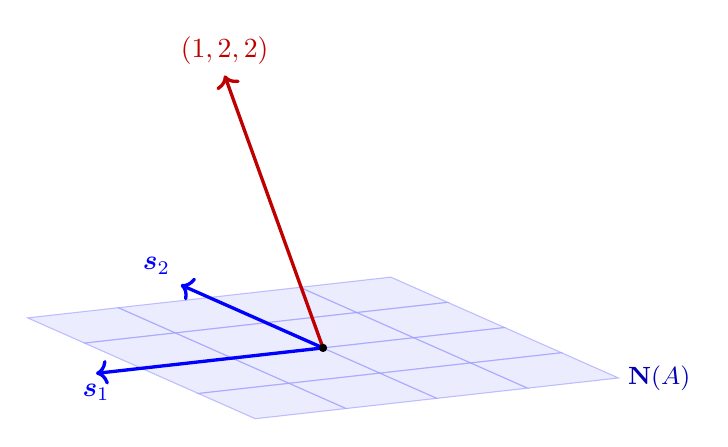
\begin{tikzpicture}
\begin{axis}[view={-50}{15}, width=9.5cm, height=9.5cm, axis lines=none,
  xmin=-2, xmax=2, ymin=-2, ymax=2, zmin=-2, zmax=2, clip=false,
  unit vector ratio=1 1 1]
  \addplot3[surf, shader=faceted, colormap={single}{color=(blue!12) color=(blue!12)},
    faceted color=blue!40, opacity=0.6, samples=5, domain=-0.8:0.8, y domain=-0.8:0.8]
    ({-2*x-2*y},{x},{y});
  \draw[->,very thick,blue] (0,0,0) -- (-2,1,0) node[below] {$\vb{s}_1$};
  \draw[->,very thick,blue] (0,0,0) -- (-2,0,1) node[above left] {$\vb{s}_2$};
  \draw[->,very thick,red!75!black] (0,0,0) -- (1,2,2) node[above] {$(1,2,2)$};
  \fill (0,0,0) circle (1.5pt);
  \node[blue!70!black,font=\small] at (3.2,-0.8,-0.8) [right] {$\Nul{A}$};
\end{axis}
\end{tikzpicture}
\qquad
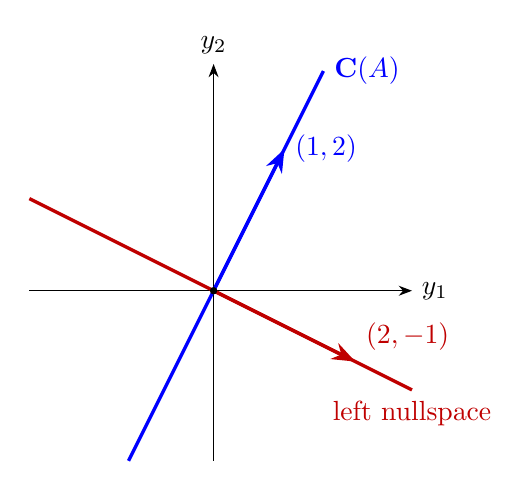
\begin{tikzpicture}[scale=0.9,>=Stealth]
  \draw[->] (-2.6,0) -- (2.8,0) node[right] {$y_1$};
  \draw[->] (0,-2.4) -- (0,3.2) node[above] {$y_2$};
  \draw[very thick,blue] (-1.2,-2.4) -- (1.55,3.1) node[right] {$\Col{A}$};
  \draw[very thick,red!75!black] (-2.6,1.3) -- (2.8,-1.4) node[below] {left nullspace};
  \draw[->,very thick,blue] (0,0) -- (1,2) node[right] {$(1,2)$};
  \draw[->,very thick,red!75!black] (0,0) -- (2,-1) node[above right] {$(2,-1)$};
  \fill (0,0) circle (1.5pt);
\end{tikzpicture}
\caption{The matrix $A=\begin{bmatrix} 1&2&2\\ 2&4&4\end{bmatrix}$. Left (inputs, $\R^3$): the
nullspace is the plane spanned by $\vb{s}_1=(-2,1,0)$ and $\vb{s}_2=(-2,0,1)$; the row
vector $(1,2,2)$ is perpendicular to it. Right (outputs, $\R^2$):
every $A\vb{x}$, including $A(-1,3,2)=(9,18)$, lies on the column-space line through $(1,2)$;
the perpendicular line through $(2,-1)$ is the left nullspace.}\label{fig:u07-crush}
\end{figure}

\subsection{Exercises}

\begin{exercise}\label{ex:u07-sum}
Let $S$ and $T$ be subspaces of a vector space $V$. Their \emph{sum} $S+T$ is the set of all
vectors $\vb{s}+\vb{t}$ with $\vb{s}\in S$ and $\vb{t}\in T$. (a) Show that $S+T$ is a subspace.
(b) If $S$ and $T$ are two different lines through the origin in $\R^m$, how do $S+T$ and
$S\cup T$ differ? Explain why the set of all combinations of vectors in $S\cup T$ is $S+T$.
\end{exercise}
\begin{solution}
(a) $\vb{0}=\vb{0}+\vb{0}\in S+T$. If $\vb{s}+\vb{t}$ and $\vb{s}'+\vb{t}'$ are in $S+T$ and $c$ is
a scalar, then $(\vb{s}+\vb{t})+(\vb{s}'+\vb{t}')=(\vb{s}+\vb{s}')+(\vb{t}+\vb{t}')$ and
$c(\vb{s}+\vb{t})=c\vb{s}+c\vb{t}$, with $\vb{s}+\vb{s}',c\vb{s}\in S$ and $\vb{t}+\vb{t}',c\vb{t}\in T$.
So $S+T$ is closed under both operations.
(b) $S\cup T$ is just the two lines, while $S+T$ is the whole plane containing them. Every
combination of vectors from $S\cup T$ can be grouped as (a vector of $S$) $+$ (a vector of
$T$), so it lies in $S+T$; conversely each $\vb{s}+\vb{t}$ is such a combination. Hence the
combinations of $S\cup T$ are exactly $S+T$, the smallest subspace containing both lines.
\end{solution}

\begin{exercise}\label{ex:u07-plane}
The plane $x-3y-z=12$ is parallel to the plane $x-3y-z=0$, and $(12,0,0)$ lies on it. Write
every point of the plane in the form
$(x,y,z)=(\,\cdot\,,0,0)+y(\,\cdot\,,1,0)+z(\,\cdot\,,0,1)$. Which part is a particular solution
and which part is the nullspace of $\begin{bmatrix} 1&-3&-1\end{bmatrix}$?
\end{exercise}
\begin{solution}
Solve for $x$: $x=12+3y+z$. So
\[
  \begin{bmatrix} x\\ y\\ z\end{bmatrix}=\begin{bmatrix} 12+3y+z\\ y\\ z\end{bmatrix}
  =\begin{bmatrix} 12\\ 0\\ 0\end{bmatrix}+y\begin{bmatrix} 3\\ 1\\ 0\end{bmatrix}
   +z\begin{bmatrix} 1\\ 0\\ 1\end{bmatrix}.
\]
The vector $(12,0,0)$ is a particular solution of $x-3y-z=12$; the combinations of $(3,1,0)$
and $(1,0,1)$ form the plane $x-3y-z=0$, the nullspace of $\begin{bmatrix} 1&-3&-1\end{bmatrix}$.
This is Proposition~\ref{prop:u07-allsolutions} for a $1\times3$ matrix.
\end{solution}

\begin{exercise}\label{ex:u07-stack}
If $C=\begin{bmatrix} A\\ B\end{bmatrix}$ is the matrix formed by placing the rows of $B$ below
the rows of $A$ (both with $n$ columns), how is $\Nul{C}$ related to $\Nul{A}$ and $\Nul{B}$?
\end{exercise}
\begin{solution}
By block multiplication $C\vb{x}=\begin{bmatrix} A\vb{x}\\ B\vb{x}\end{bmatrix}$, which is zero
exactly when $A\vb{x}=\vb{0}$ and $B\vb{x}=\vb{0}$. So $\Nul{C}=\Nul{A}\cap\Nul{B}$, the
vectors in both nullspaces. (This is a subspace, as Theorem~\ref{thm:u07-intersection}
guarantees: stacking more equations can only shrink the nullspace.)
\end{solution}

\begin{exercise}\label{ex:u07-which}
Which of these subsets of $\R^3$ are subspaces? (a) all $\vb{b}$ with $b_1+b_2-b_3=0$;
(b) all $\vb{b}$ with $b_3=b_1b_2$; (c) all $\vb{b}=c_1(1,0,-1)+c_2(1,0,1)+(1,0,0)$;
(d) all $\vb{b}=c_1(1,0,-1)+c_2(1,0,1)+(0,1,0)$, where $c_1,c_2$ range over $\R$.
\end{exercise}
\begin{solution}
(a) Yes: it is the nullspace of the $1\times3$ matrix $\begin{bmatrix} 1&1&-1\end{bmatrix}$.
(b) No: $(1,1,1)$ is in the set ($1=1\cdot1$), but $2(1,1,1)=(2,2,2)$ is not ($2\neq2\cdot2$).
(c) Yes: $(1,0,0)=\tfrac12(1,0,-1)+\tfrac12(1,0,1)$ already lies in the plane spanned by the two
vectors, so $\vb{b}=(c_1+\tfrac12)(1,0,-1)+(c_2+\tfrac12)(1,0,1)$ runs over exactly that plane
(the plane $b_2=0$), a subspace.
(d) No: every vector in the span of $(1,0,-1)$ and $(1,0,1)$ has second component $0$, so every
$\vb{b}$ in the set has $b_2=1$. The zero vector is not in the set.
\end{solution}

\begin{exercise}\label{ex:u07-practice}
Change the last entry of Example~\ref{ex:u07-crush}: $A=\begin{bmatrix} 1&2&2\\ 2&4&5\end{bmatrix}$.
How many pivots are there now, what is $\Nul{A}$, and what is $\Col{A}$?
\end{exercise}
\begin{solution}
Row~2 $-$ 2 row~1 $=(0,0,1)$, so there are two pivots, in columns~1 and~3 ($r=2$). The
equations $x_1+2x_2+2x_3=0$ and $x_3=0$ give $x_1=-2x_2$, so $\Nul{A}$ is the line of multiples
of $(-2,1,0)$, of dimension $3-2=1$. Columns~1 and~3, $(1,2)$ and $(2,5)$, are not parallel,
so their combinations fill the plane: $\Col{A}=\R^2$, and $A\vb{x}=\vb{b}$ is solvable for
every $\vb{b}$.
\end{solution}

% unit: u08
% sources: sources/014-solving-ax-0-pivot-variables-special-solutions.txt, sources/024-solving-ax-0-pivot-variables-special-solutions.txt, sources/107-mit18-06scf11-ses1-7sum-pdf-download-file.txt, sources/108-solving-ax-0.txt, sources/109-mit18-06scf11-ses1-7prob-pdf-download-file.txt, sources/110-mit18-06scf11-ses1-7sol-pdf-download-file.txt
\section{\texorpdfstring{Solving \(A\vb{x}=\vb{0}\): pivot variables, special solutions}{Solving Ax = 0: pivot variables, special solutions}}\label{sec:u08}

Section~\ref{sec:u07} defined the nullspace $\Nul{A}$ as the set of all solutions of
$A\vb{x}=\vb{0}$ and showed that it is a subspace of $\R^n$. A definition is not yet a
description: we want to \emph{list} what is in $\Nul{A}$. This section turns elimination, which
so far solved square invertible systems, into an algorithm that works for every $m\times n$
matrix. The algorithm produces one number, the rank $r$, and a short list of $n-r$
\emph{special solutions} whose combinations are exactly the nullspace.

\subsection{Elimination on a rectangular matrix}

The running example of the lecture is the $3\times 4$ matrix
\[
A=\begin{bmatrix}1&2&2&2\\2&4&6&8\\3&6&8&10\end{bmatrix}.
\]
Two facts are visible before any computation: column~2 is twice column~1, and row~3 is
row~1 plus row~2. Elimination should discover both. The first question is whether elimination
is allowed to change the problem.

\begin{proposition}[Row operations keep the nullspace]\label{prop:u08-same-null}
If $E$ is an invertible $m\times m$ matrix, then $\Nul{EA}=\Nul{A}$. In particular, subtracting
a multiple of one row from another, exchanging two rows, or dividing a row by a nonzero number
never changes the nullspace.
\end{proposition}
\begin{proof}
If $A\vb{x}=\vb{0}$ then $EA\vb{x}=E\vb{0}=\vb{0}$. Conversely, if $EA\vb{x}=\vb{0}$, multiply on
the left by $E^{-1}$ to get $A\vb{x}=\vb{0}$. Each elimination step is multiplication on the left
by an invertible elementary or permutation matrix (Sections~\ref{sec:u03} and~\ref{sec:u06}), and
a product of invertible matrices is invertible.
\end{proof}

Because the right-hand side is $\vb{0}$ and stays $\vb{0}$ under every row operation, we do not
need to carry it along. Elimination proceeds column by column as in the square case, with one
new rule: if the pivot position and every entry below it are zero, there is nothing to do in
that column, so we move to the next column (staying in the same row) instead of stopping.

\begin{example}[Elimination with a missing pivot]\label{ex:u08-elim}
Subtract $2\times$row~1 from row~2 and $3\times$row~1 from row~3:
\[
\begin{bmatrix}1&2&2&2\\2&4&6&8\\3&6&8&10\end{bmatrix}\longrightarrow
\begin{bmatrix}1&2&2&2\\0&0&2&4\\0&0&2&4\end{bmatrix}.
\]
In column~2 the pivot position $(2,2)$ holds a zero and so does the entry below it, so no row
exchange can help: column~2 gets no pivot. The next pivot is the $2$ in row~2, column~3.
Subtracting row~2 from row~3 finishes the job:
\[
U=\begin{bmatrix}\boxed{1}&2&2&2\\0&0&\boxed{2}&4\\0&0&0&0\end{bmatrix}.
\]
The row of zeros records that row~3 of $A$ was a combination of rows~1 and~2; elimination
knocked it out.
\end{example}

\begin{definition}[Echelon form, pivots, rank]\label{def:u08-rank}
A matrix is in \emph{echelon form} if every zero row lies below all nonzero rows and the first
nonzero entry of each nonzero row (its \emph{pivot}) lies strictly to the right of the pivot in
the row above. Elimination brings every matrix $A$ to an echelon form $U$. The \emph{rank} of
$A$, written $r=\rank A$, is the number of pivots. Columns that contain a pivot are
\emph{pivot columns}; the remaining columns are \emph{free columns}.
\end{definition}

A row holds at most one pivot and so does a column, so always
\[
r\le m\qquad\text{and}\qquad r\le n.
\]
In Example~\ref{ex:u08-elim} the rank is $2$, the pivot columns are $1$ and $3$, and the free
columns are $2$ and $4$. (That the rank does not depend on the order of the elimination steps
follows from Section~\ref{sec:u10}, where $r$ is identified with the dimension of the column
space, a number defined without elimination.)

\subsection{Pivot variables, free variables and special solutions}

The system $U\vb{x}=\vb{0}$ of Example~\ref{ex:u08-elim} is
\begin{align*}
x_1+2x_2+2x_3+2x_4&=0,\\
2x_3+4x_4&=0.
\end{align*}
The unknowns that multiply pivot columns, $x_1$ and $x_3$, are \emph{pivot variables}; the
others, $x_2$ and $x_4$, are \emph{free variables}. The free variables may be given any values.
Once they are chosen, back substitution determines the pivot variables uniquely, because each
nonzero row, read from the bottom up, contains exactly one new pivot variable with a nonzero
coefficient.

\begin{definition}[Special solutions]\label{def:u08-special}
For each free variable, the \emph{special solution} is the solution of $A\vb{x}=\vb{0}$ in
which that free variable equals $1$, every other free variable equals $0$, and the pivot
variables are found by back substitution.
\end{definition}

\begin{example}[The two special solutions]\label{ex:u08-special}
Take $x_2=1$, $x_4=0$. The second equation gives $2x_3=0$, so $x_3=0$; the first gives
$x_1+2=0$, so $x_1=-2$. Next take $x_2=0$, $x_4=1$. Then $2x_3+4=0$ gives $x_3=-2$, and
$x_1+2(-2)+2=0$ gives $x_1=2$:
\[
\vb{s}_1=\begin{bmatrix}-2\\1\\0\\0\end{bmatrix},\qquad
\vb{s}_2=\begin{bmatrix}2\\0\\-2\\1\end{bmatrix}.
\]
Each special solution is a dependency among the columns of $A$. The first says
$-2(\text{col }1)+(\text{col }2)=\vb{0}$: column~2 is twice column~1. The second says
$2(\text{col }1)-2(\text{col }3)+(\text{col }4)=\vb{0}$, and indeed
$2(1,2,3)-2(2,6,8)+(2,8,10)=(0,0,0)$. The whole nullspace is
\[
\Nul{A}=\{\,c\,\vb{s}_1+d\,\vb{s}_2 : c,d\in\R\,\},
\]
a two-dimensional plane through the origin in $\R^4$.
\end{example}

\begin{theorem}[Special solutions describe the nullspace]\label{thm:u08-special}
Let $A$ be $m\times n$ with rank $r$. There are exactly $n-r$ special solutions
$\vb{s}_1,\dots,\vb{s}_{n-r}$, and $\Nul{A}$ consists of all their linear combinations. More
precisely, if $\vb{x}\in\Nul{A}$ and its free variables have the values $c_1,\dots,c_{n-r}$,
then $\vb{x}=c_1\vb{s}_1+\dots+c_{n-r}\vb{s}_{n-r}$.
\end{theorem}
\begin{proof}
There are $r$ pivot columns, hence $n-r$ free columns and one special solution for each. The
special solutions lie in $\Nul{A}$, which is a subspace, so all their combinations do too.

Conversely, let $\vb{x}\in\Nul{A}$ have free variables $c_1,\dots,c_{n-r}$ and put
$\vb{y}=\vb{x}-\sum_j c_j\vb{s}_j$. Then $\vb{y}\in\Nul{A}=\Nul{U}$ by
Proposition~\ref{prop:u08-same-null}. Since $\vb{s}_j$ has a $1$ in the $j$th free position and
$0$ in the other free positions, every free variable of $\vb{y}$ is $0$. Now solve
$U\vb{y}=\vb{0}$ from the last nonzero row upward. In that row every entry to the right of the
pivot multiplies a free variable, which is zero, so the pivot variable is zero. In each row above,
the entries to the right of the pivot multiply free variables or pivot variables already shown to
be zero, so that row's pivot variable is zero as well. Hence $\vb{y}=\vb{0}$, that is,
$\vb{x}=\sum_j c_j\vb{s}_j$.
\end{proof}

\begin{corollary}[More unknowns than equations]\label{cor:u08-wide}
If $n>m$, then $A\vb{x}=\vb{0}$ has a solution $\vb{x}\ne\vb{0}$.
\end{corollary}
\begin{proof}
Since $r\le m<n$, there is at least one free variable, and its special solution has a $1$ in
that position.
\end{proof}

\subsection{The reduced row echelon form \texorpdfstring{\(R\)}{R}}

Elimination can go further. Working upward, we can also clear the entries \emph{above} each pivot
and then divide each pivot row by its pivot.

\begin{definition}[Reduced row echelon form]\label{def:u08-rref}
A matrix is in \emph{reduced row echelon form} if it is in echelon form, every pivot equals $1$,
and every pivot is the only nonzero entry in its column. Elimination brings every matrix $A$ to
such a matrix, and (a standard fact we use without proof) the result does not depend on the order
of the steps; it is denoted $R=\operatorname{rref}(A)$ (MATLAB: \texttt{rref(A)}).
\end{definition}

\begin{example}[From \texorpdfstring{\(U\)}{U} to \texorpdfstring{\(R\)}{R}]\label{ex:u08-rref}
In $U$ from Example~\ref{ex:u08-elim}, subtract row~2 from row~1 to clear the $2$ above the
second pivot, then divide row~2 by its pivot $2$:
\[
U=\begin{bmatrix}1&2&2&2\\0&0&2&4\\0&0&0&0\end{bmatrix}\longrightarrow
\begin{bmatrix}1&2&0&-2\\0&0&2&4\\0&0&0&0\end{bmatrix}\longrightarrow
R=\begin{bmatrix}1&2&0&-2\\0&0&1&2\\0&0&0&0\end{bmatrix}.
\]
The equations $R\vb{x}=\vb{0}$ are $x_1=-2x_2+2x_4$ and $x_3=-2x_4$: the pivot variables are
written directly in terms of the free ones. The free columns of $R$ contain $(2,0)$ and
$(-2,2)$ in the pivot rows, and these numbers reappear in $\vb{s}_1$ and $\vb{s}_2$ with their
signs reversed: $(x_1,x_3)=(-2,0)$ and $(2,-2)$.
\end{example}

The sign reversal is no accident. Suppose for the moment that the pivot columns come first (this
is only a renaming of the unknowns). Then $R$ has an identity block in its pivot rows and pivot
columns, a block $F$ in its pivot rows and free columns, and zero rows below:
\[
R=\begin{bmatrix}I&F\\0&0\end{bmatrix},\qquad I\text{ is }r\times r,\quad F\text{ is }r\times(n-r).
\]

\begin{proposition}[The nullspace matrix]\label{prop:u08-nullmatrix}
With $R$ in this block form, the $n\times(n-r)$ matrix
\[
N=\begin{bmatrix}-F\\ I\end{bmatrix}\qquad(\text{here }I\text{ is }(n-r)\times(n-r))
\]
satisfies $RN=0$, and its columns are the special solutions.
\end{proposition}
\begin{proof}
Block multiplication gives $RN=\begin{bmatrix}I(-F)+F\,I\\ 0\end{bmatrix}=0$. Column $j$ of $N$
has free part equal to column $j$ of the identity, a $1$ in the $j$th free position and zeros
in the others, so it is the solution whose free variables are those of the $j$th special
solution. Since back substitution determines the pivot variables uniquely, it \emph{is} the
$j$th special solution. Equivalently: $R\vb{x}=\vb{0}$ says
$\vb{x}_{\text{pivot}}+F\vb{x}_{\text{free}}=\vb{0}$, so $\vb{x}_{\text{pivot}}=-F\vb{x}_{\text{free}}$.
\end{proof}

When the pivot columns are not first, put the rows of $-F$ in the pivot positions and the rows
of $I$ in the free positions. In Example~\ref{ex:u08-rref}, $F=\begin{bmatrix}2&-2\\0&2\end{bmatrix}$
(rows~1--2, columns~2 and~4), so rows~1 and~3 of $N$ come from $-F$ and rows~2 and~4 from $I$:
\[
N=\begin{bmatrix}-2&2\\1&0\\0&-2\\0&1\end{bmatrix}=\begin{bmatrix}\vb{s}_1&\vb{s}_2\end{bmatrix}.
\]
Figure~\ref{fig:u08-blocks} records the shapes; this is exactly what the teaching code
\texttt{null(A)} does after computing $R$.

\begin{figure}[ht]\centering
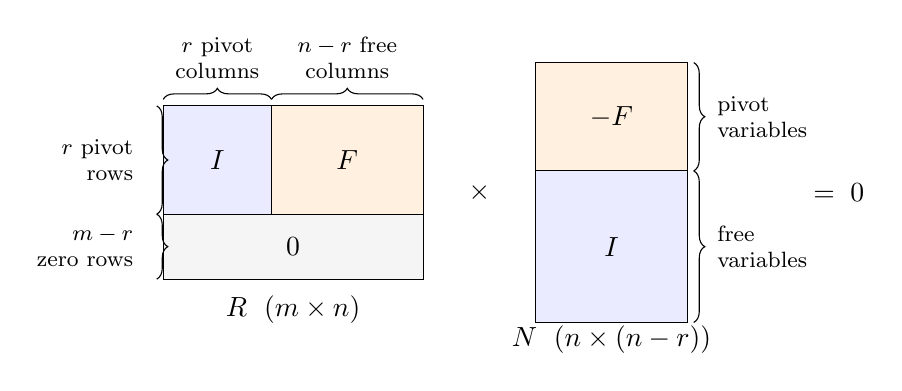
\begin{tikzpicture}[scale=0.55,>=Stealth]
  % R: m = 4 rows (r = 2.5 + 1.5), n = 6 columns (r = 2.5 + 3.5)
  \draw[fill=blue!8] (0,1.5) rectangle (2.5,4);
  \draw[fill=orange!12] (2.5,1.5) rectangle (6,4);
  \draw[fill=gray!8] (0,0) rectangle (6,1.5);
  \node at (1.25,2.75) {$I$};
  \node at (4.25,2.75) {$F$};
  \node at (3,0.75) {$0$};
  \draw[decorate,decoration={brace,amplitude=4pt}] (0,4.15) -- (2.5,4.15)
    node[midway,above=4pt,font=\footnotesize,align=center] {$r$ pivot\\columns};
  \draw[decorate,decoration={brace,amplitude=4pt}] (2.5,4.15) -- (6,4.15)
    node[midway,above=4pt,font=\footnotesize,align=center] {$n-r$ free\\columns};
  \draw[decorate,decoration={brace,amplitude=4pt,mirror}] (-0.15,1.5) -- (-0.15,4)
    node[midway,left=5pt,font=\footnotesize,align=right] {$r$ pivot\\rows};
  \draw[decorate,decoration={brace,amplitude=4pt,mirror}] (-0.15,0) -- (-0.15,1.5)
    node[midway,left=5pt,font=\footnotesize,align=right] {$m-r$\\zero rows};
  \node at (3,-0.7) {$R$ \;($m\times n$)};
  % N: n = 6 rows (2.5 + 3.5), n - r = 3.5 columns
  \begin{scope}[xshift=8.6cm,yshift=-1cm]
    \draw[fill=orange!12] (0,3.5) rectangle (3.5,6);
    \draw[fill=blue!8] (0,0) rectangle (3.5,3.5);
    \node at (1.75,4.75) {$-F$};
    \node at (1.75,1.75) {$I$};
    \draw[decorate,decoration={brace,amplitude=4pt}] (3.65,6) -- (3.65,3.5)
      node[midway,right=5pt,font=\footnotesize,align=left] {pivot\\variables};
    \draw[decorate,decoration={brace,amplitude=4pt}] (3.65,3.5) -- (3.65,0)
      node[midway,right=5pt,font=\footnotesize,align=left] {free\\variables};
    \node at (1.75,-0.4) {$N$ \;($n\times(n-r)$)};
  \end{scope}
  \node at (7.3,2) {$\times$};
  \node at (15.6,2) {$=\;0$};
\end{tikzpicture}
\caption{Block shapes in $RN=0$ when the pivot columns come first. Each column of $N$ is a
special solution: the identity block sets one free variable to $1$ and the others to $0$, and
$-F$ supplies the pivot variables, so that $I(-F)+F\,I=0$.}
\label{fig:u08-blocks}
\end{figure}

\subsection{Two more examples}

\begin{example}[The transpose needs a row exchange]\label{ex:u08-transpose}
Take $A\T=\begin{bmatrix}1&2&3\\2&4&6\\2&6&8\\2&8&10\end{bmatrix}$. Its third column is the
sum of the first two, so we expect a free third column. Subtract $2\times$row~1 from rows 2, 3
and~4; column~2 then has a zero in the pivot position but a $2$ below it, so exchange rows~2
and~3; finally subtract $2\times$row~2 from row~4:
\[
\begin{bmatrix}1&2&3\\0&0&0\\0&2&2\\0&4&4\end{bmatrix}\longrightarrow
\begin{bmatrix}1&2&3\\0&2&2\\0&0&0\\0&4&4\end{bmatrix}\longrightarrow
U=\begin{bmatrix}1&2&3\\0&2&2\\0&0&0\\0&0&0\end{bmatrix}.
\]
Column~3 has nothing in the pivot position or below, so the rank is $2$, the same as the rank
of $A$; Section~\ref{sec:u11} proves that $\rank A\T=\rank A$ always. With the free variable
$x_3=1$, the second row gives $2x_2+2=0$, so $x_2=-1$, and the first gives $x_1-2+3=0$, so
$x_1=-1$. The nullspace is the line $\{c(-1,-1,1)\}$ in $\R^3$. Going on to
$R=\begin{bmatrix}1&0&1\\0&1&1\\0&0&0\\0&0&0\end{bmatrix}$ shows $F=\begin{bmatrix}1\\1\end{bmatrix}$
and $N=\begin{bmatrix}-F\\1\end{bmatrix}=(-1,-1,1)$, as it must.
\end{example}

\begin{example}[What a matrix crushes]\label{ex:u08-crush}
Let $A=\begin{bmatrix}1&2&2\\2&4&4\end{bmatrix}$, which takes $n=3$ inputs to $m=2$ outputs.
Row~2 minus $2\times$row~1 is $(0,0,0)$, so $R=\begin{bmatrix}1&2&2\\0&0&0\end{bmatrix}$ has one
pivot and $r=1$. The free columns $2$ and~$3$ give
\[
\vb{s}_1=\begin{bmatrix}-2\\1\\0\end{bmatrix},\qquad \vb{s}_2=\begin{bmatrix}-2\\0\\1\end{bmatrix},
\qquad A\vb{s}_1=\begin{bmatrix}-2+2\\-4+4\end{bmatrix}=\vb{0},\quad
A\vb{s}_2=\begin{bmatrix}-2+2\\-4+4\end{bmatrix}=\vb{0}.
\]
So $\Nul{A}$ is a plane in $\R^3$ of dimension $n-r=2$: a whole plane of inputs is sent to
zero. Both special solutions are perpendicular to the row $(1,2,2)$, since
$-2+2+0=0$ and $-2+0+2=0$. That is no coincidence: $A\vb{x}=\vb{0}$ says precisely that
$\vb{x}$ has zero dot product with every row. Section~\ref{sec:u11} completes this example with
the other three subspaces.
\end{example}

\begin{trap}
Row operations preserve the nullspace but \emph{not} the column space. In
Example~\ref{ex:u08-elim}, column~3 of $U$ is $(2,2,0)$. Every vector $A\vb{x}$ has third component
equal to the sum of the first two (row~3 of $A$ is row~1 plus row~2), and $2+2\ne 0$, so $(2,2,0)$
is not in $\Col{A}$. Use $U$ or $R$ to find $\Nul{A}$ and to locate the pivot columns, but take
those pivot columns from the original $A$ when you want the column space. A second slip: setting
\emph{all} free variables to zero produces only $\vb{x}=\vb{0}$; a special solution needs a $1$.
\end{trap}

\subsection{Exercises}

\begin{exercise}\label{exr:u08-rref}
Let $A=\begin{bmatrix}1&5&7&9\\0&4&1&7\\2&-2&11&-3\end{bmatrix}$. (a) Find the reduced row
echelon form of $A$. (b) What is the rank of $A$? (c) Find the special solutions of
$A\vb{x}=\vb{0}$.
\end{exercise}
\begin{solution}
(a) Subtract $2\times$row~1 from row~3, giving row~3 $=(0,-12,-3,-21)$. Divide row~2 by $4$:
$(0,1,\tfrac14,\tfrac74)$. Add $12\times$(new row~2) to row~3, giving a zero row. Subtract
$5\times$row~2 from row~1: $7-\tfrac54=\tfrac{23}{4}$ and $9-\tfrac{35}{4}=\tfrac14$. Hence
\[
R=\begin{bmatrix}1&0&\tfrac{23}{4}&\tfrac14\\[2pt]0&1&\tfrac14&\tfrac74\\[2pt]0&0&0&0\end{bmatrix}.
\]
(b) There are two pivots, so $\rank A=2$.
(c) The free variables are $x_3,x_4$, and $F=\begin{bmatrix}23/4&1/4\\1/4&7/4\end{bmatrix}$.
The columns of $\begin{bmatrix}-F\\I\end{bmatrix}$ are
$\vb{s}_1=\bigl(-\tfrac{23}{4},-\tfrac14,1,0\bigr)$ and $\vb{s}_2=\bigl(-\tfrac14,-\tfrac74,0,1\bigr)$.
Check one entry: row~2 of $A$ times $\vb{s}_1$ is $4(-\tfrac14)+1=0$.
\end{solution}

\begin{exercise}\label{exr:u08-change}
Change one entry of Example~\ref{ex:u08-crush}: $A=\begin{bmatrix}1&2&2\\2&4&5\end{bmatrix}$.
Find the rank, the special solutions and the dimension of the nullspace.
\end{exercise}
\begin{solution}
Row~2 minus $2\times$row~1 is now $(0,0,1)$, so there are pivots in columns~1 and~3 and $r=2$.
Clearing above the second pivot gives $R=\begin{bmatrix}1&2&0\\0&0&1\end{bmatrix}$. The only free
variable is $x_2$; setting $x_2=1$ gives $x_3=0$ and $x_1=-2$. The nullspace is the line through
$(-2,1,0)$, of dimension $3-2=1$: the plane of Example~\ref{ex:u08-crush} has shrunk to a line.
\end{solution}

\begin{exercise}\label{exr:u08-reverse}
Find a $2\times 4$ matrix $R$ in reduced row echelon form whose special solutions are
$(-3,1,0,0)$ and $(-2,0,-6,1)$.
\end{exercise}
\begin{solution}
In a special solution the free variables are $1$ and $0$; here the pattern
$(x_2,x_4)=(1,0)$ and $(0,1)$ shows that $x_2,x_4$ are free and $x_1,x_3$ are pivot variables.
By Proposition~\ref{prop:u08-nullmatrix} the pivot entries of the special solutions are the
columns of $-F$: $(x_1,x_3)=(-3,0)$ and $(-2,-6)$, so $F$ has columns $(3,0)$ and $(2,6)$.
Placing the identity in columns~1 and~3 and $F$ in columns~2 and~4,
\[
R=\begin{bmatrix}1&3&0&2\\0&0&1&6\end{bmatrix}.
\]
Check: $R(-3,1,0,0)=(-3+3,\,0)=\vb{0}$ and $R(-2,0,-6,1)=(-2+2,\,-6+6)=\vb{0}$.
\end{solution}

\begin{exercise}\label{exr:u08-rankAB}
Let $B=\begin{bmatrix}1&1\\1&1\end{bmatrix}$. Find $2\times2$ matrices $A_1$ and $A_2$ with
$\rank(A_1B)=1$ and $\rank(A_2B)=0$, and describe all possible $A_2$.
\end{exercise}
\begin{solution}
$A_1=I$ works: $A_1B=B$ has equal rows, so elimination leaves one pivot. $A_2=0$ works
trivially. In general, a row $(a,b)$ of $A_2$ multiplies $B$ to give $(a+b,\,a+b)$, which is zero
exactly when $b=-a$. So $A_2B=0$ precisely when every row of $A_2$ is a multiple of $(1,-1)$, for
example $A_2=\begin{bmatrix}1&-1\\1&-1\end{bmatrix}$.
\end{solution}

% unit: u09
% sources: sources/093-solving-ax-b-row-reduced-form-r.txt, sources/147-solving-ax-b-row-reduced-form-r.txt, sources/148-mit18-06scf11-ses1-8sum-pdf-download-file.txt, sources/149-solving-ax-b.txt, sources/150-mit18-06scf11-ses1-8prob-pdf-download-file.txt, sources/151-mit18-06scf11-ses1-8sol-pdf-download-file.txt
\section{\texorpdfstring{Solving \(A\vb{x}=\vb{b}\): row reduced form \(R\)}{Solving Ax = b: row reduced form R}}\label{sec:u09}

Section~\ref{sec:u08} found every solution of $A\vb{x}=\vb{0}$. Now the right-hand side is a
general vector $\vb{b}\in\R^m$, and three questions arise: \emph{is there} a solution, \emph{how
do we find one}, and \emph{what are all of them}? Elimination answers all three. A solution
exists only when $\vb{b}$ passes a test that elimination produces; every solution is one
particular solution plus a vector from the nullspace; and the rank $r$ alone predicts whether there
are $0$, $1$ or infinitely many solutions.

\subsection{When is \texorpdfstring{\(A\vb{x}=\vb{b}\)}{Ax = b} solvable?}

Keep the matrix of Section~\ref{sec:u08}, whose third row is the sum of the first two:
\[
A=\begin{bmatrix}1&2&2&2\\2&4&6&8\\3&6&8&10\end{bmatrix}.
\]
Adding the first two equations of $A\vb{x}=\vb{b}$ gives the left side of the third, so a solution
can exist only if $b_1+b_2=b_3$. With $\vb{b}=(1,5,17)$ there is no solution; with $b_1=1$, $b_2=5$
the only acceptable third component is $b_3=6$.

Elimination discovers this condition by itself. We attach $\vb{b}$ as an extra column, forming
the \emph{augmented matrix} $\begin{bmatrix}A&\vb{b}\end{bmatrix}$, and do to the last column
whatever we do to the rows of $A$:
\[
\left[\begin{array}{cccc|c}1&2&2&2&b_1\\2&4&6&8&b_2\\3&6&8&10&b_3\end{array}\right]
\longrightarrow
\left[\begin{array}{cccc|c}1&2&2&2&b_1\\0&0&2&4&b_2-2b_1\\0&0&2&4&b_3-3b_1\end{array}\right]
\longrightarrow
\left[\begin{array}{cccc|c}1&2&2&2&b_1\\0&0&2&4&b_2-2b_1\\0&0&0&0&b_3-b_2-b_1\end{array}\right].
\]
The last row is the equation $0=b_3-b_2-b_1$. If a row of $A$ is wiped out, the same
combination of the entries of $\vb{b}$ must vanish. For $\vb{b}=(1,5,6)$ the last column becomes
$(1,3,0)$ and the system is consistent.

There are now two descriptions of the good right-hand sides. Section~\ref{sec:u07} said that
$A\vb{x}=\vb{b}$ is solvable exactly when $\vb{b}\in\Col{A}$, because $A\vb{x}$ is the combination
of the columns with weights $x_1,\dots,x_n$. Elimination says: whenever a combination of the
rows gives the zero row, the same combination of the $b_i$ must give zero. These are not
obviously the same, but they are.

\begin{theorem}[Solvability]\label{thm:u09-solvable}
For an $m\times n$ matrix $A$ and $\vb{b}\in\R^m$ the following are equivalent:
\begin{enumerate}[(a)]
\item $A\vb{x}=\vb{b}$ has a solution;
\item $\vb{b}\in\Col{A}$;
\item $\vb{y}\T\vb{b}=0$ for every $\vb{y}\in\R^m$ with $\vb{y}\T A=\vb{0}\T$ (every combination of
rows that gives the zero row also gives zero when applied to $\vb{b}$).
\end{enumerate}
\end{theorem}
\begin{proof}
(a)$\Leftrightarrow$(b): $A\vb{x}=x_1\vb{a}_1+\dots+x_n\vb{a}_n$, so $A\vb{x}=\vb{b}$ asks
exactly for weights that produce $\vb{b}$ from the columns.

(a)$\Rightarrow$(c): if $A\vb{x}=\vb{b}$ and $\vb{y}\T A=\vb{0}\T$, then
$\vb{y}\T\vb{b}=\vb{y}\T A\vb{x}=\vb{0}\T\vb{x}=0$.

(c)$\Rightarrow$(a): let $E$ be the invertible matrix that records the elimination steps, so that
$EA=R$ is the reduced row echelon form, and let $r=\rank A$. Then $A\vb{x}=\vb{b}$ is equivalent
to $R\vb{x}=E\vb{b}$. For $i>r$, row $i$ of $R$ is zero, so the $i$th row $\vb{y}_i\T$ of $E$
satisfies $\vb{y}_i\T A=\vb{0}\T$, and by (c) the $i$th entry of $E\vb{b}$, namely
$\vb{y}_i\T\vb{b}$, is $0$. Hence the zero rows of $R\vb{x}=E\vb{b}$ read $0=0$. In the first
$r$ rows, set every free variable to $0$; since the pivot columns of $R$ are columns of the
identity, the $i$th pivot variable equals the $i$th entry of $E\vb{b}$. This $\vb{x}$ solves
$R\vb{x}=E\vb{b}$, hence $A\vb{x}=E^{-1}R\vb{x}=E^{-1}E\vb{b}=\vb{b}$.
\end{proof}

The vectors $\vb{y}$ in (c) form the left nullspace $\Nul{A\T}$, the fourth of the subspaces in
Section~\ref{sec:u11}. In the example, $\vb{y}=(-1,-1,1)$ gives the condition
$-b_1-b_2+b_3=0$.

\subsection{The complete solution \texorpdfstring{\(\vb{x}_p+\vb{x}_n\)}{xp + xn}}

The proof just given also finds a solution.

\begin{definition}[Particular solution]\label{def:u09-particular}
When $A\vb{x}=\vb{b}$ is solvable, the \emph{particular solution} $\vb{x}_p$ is the solution whose
free variables are all $0$. Its pivot variables come from back substitution, or directly from the
last column of the reduced augmented matrix $\begin{bmatrix}R&\vb{d}\end{bmatrix}$.
\end{definition}

\begin{example}[A particular solution]\label{ex:u09-particular}
For $\vb{b}=(1,5,6)$, set the free variables $x_2=x_4=0$. The two remaining equations are
$x_1+2x_3=1$ and $2x_3=3$, so $x_3=\tfrac32$ and $x_1=1-3=-2$. Carrying the elimination on to
the reduced form gives the same numbers without back substitution:
\[
\left[\begin{array}{cccc|c}1&2&2&2&1\\0&0&2&4&3\\0&0&0&0&0\end{array}\right]
\longrightarrow
\left[\begin{array}{cccc|c}1&2&0&-2&-2\\0&0&1&2&\tfrac32\\0&0&0&0&0\end{array}\right]
=\begin{bmatrix}R&\vb{d}\end{bmatrix},\qquad
\vb{x}_p=\begin{bmatrix}-2\\0\\\tfrac32\\0\end{bmatrix}.
\]
The entries of $\vb{d}$ sit in the pivot positions of $\vb{x}_p$ and zeros sit in the free
positions. Check: $A\vb{x}_p=(-2+3,\,-4+9,\,-6+12)=(1,5,6)$.
\end{example}

\begin{theorem}[Complete solution]\label{thm:u09-complete}
Suppose $A\vb{x}_p=\vb{b}$. Then $\vb{x}$ solves $A\vb{x}=\vb{b}$ if and only if
$\vb{x}=\vb{x}_p+\vb{x}_n$ for some $\vb{x}_n\in\Nul{A}$.
\end{theorem}
\begin{proof}
If $\vb{x}_n\in\Nul{A}$ then $A(\vb{x}_p+\vb{x}_n)=A\vb{x}_p+A\vb{x}_n=\vb{b}+\vb{0}=\vb{b}$.
Conversely, if $A\vb{x}=\vb{b}$ then $A(\vb{x}-\vb{x}_p)=\vb{b}-\vb{b}=\vb{0}$, so
$\vb{x}_n=\vb{x}-\vb{x}_p$ lies in $\Nul{A}$ and $\vb{x}=\vb{x}_p+\vb{x}_n$.
\end{proof}

\begin{example}[All solutions for \texorpdfstring{\(\vb{b}=(1,5,6)\)}{b = (1,5,6)}]\label{ex:u09-complete}
The nullspace was found in Example~\ref{ex:u08-special}. Therefore
\[
\vb{x}_{\text{complete}}=
\begin{bmatrix}-2\\0\\\tfrac32\\0\end{bmatrix}
+c_1\begin{bmatrix}-2\\1\\0\\0\end{bmatrix}
+c_2\begin{bmatrix}2\\0\\-2\\1\end{bmatrix},\qquad c_1,c_2\in\R.
\]
There is no free constant in front of $\vb{x}_p$: tripling it would give right-hand side $3\vb{b}$.
The constants belong to the nullspace part, because only there do multiples and sums keep the
right-hand side at $\vb{0}$.
\end{example}

Geometrically, $\Nul{A}$ is a two-dimensional subspace of $\R^4$, and the solutions of
$A\vb{x}=\vb{b}$ form a copy of it shifted away from the origin so that it passes through
$\vb{x}_p$. That shifted copy is \emph{not} a subspace (it does not contain $\vb{0}$ when
$\vb{b}\neq\vb{0}$). Figure~\ref{fig:u09-planes} shows the same structure in $\R^3$.

\begin{figure}[ht]\centering
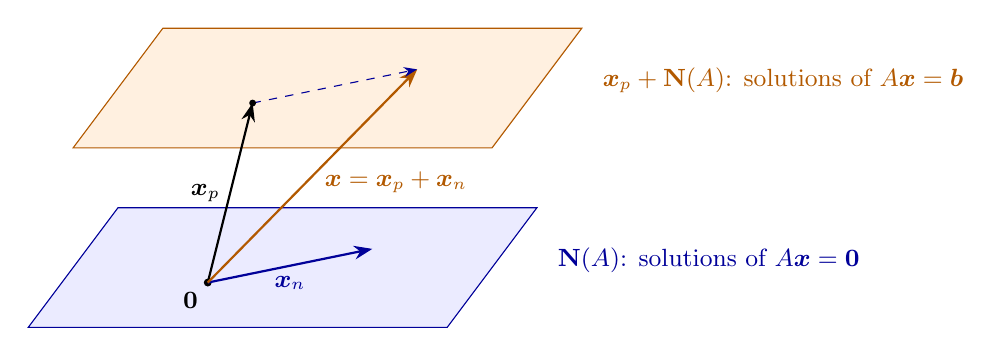
\begin{tikzpicture}[scale=0.95,>=Stealth]
  % lower plane: the nullspace
  \fill[blue!8] (-3,-0.8) -- (2.6,-0.8) -- (3.8,0.8) -- (-1.8,0.8) -- cycle;
  \draw[blue!60!black] (-3,-0.8) -- (2.6,-0.8) -- (3.8,0.8) -- (-1.8,0.8) -- cycle;
  \node[blue!60!black,anchor=west,font=\small] at (3.95,0.1) {$\Nul{A}$: solutions of $A\vb{x}=\vb{0}$};
  % upper plane: the shifted copy
  \fill[orange!12] (-2.4,1.6) -- (3.2,1.6) -- (4.4,3.2) -- (-1.2,3.2) -- cycle;
  \draw[orange!70!black] (-2.4,1.6) -- (3.2,1.6) -- (4.4,3.2) -- (-1.2,3.2) -- cycle;
  \node[orange!70!black,anchor=west,font=\small] at (4.55,2.5) {$\vb{x}_p+\Nul{A}$: solutions of $A\vb{x}=\vb{b}$};
  % vectors
  \coordinate (O) at (-0.6,-0.2);
  \coordinate (P) at (0,2.2);
  \coordinate (N) at (1.6,0.25);
  \coordinate (X) at ($(P)+(N)-(O)$);
  \fill (O) circle (1.5pt) node[below left,font=\small] {$\vb{0}$};
  \draw[->,thick] (O) -- (P) node[midway,left,font=\small] {$\vb{x}_p$};
  \draw[->,thick,blue!60!black] (O) -- (N) node[midway,below,font=\small] {$\vb{x}_n$};
  \draw[->,thick,orange!70!black] (O) -- (X) node[pos=0.47,right=3pt,font=\small] {$\vb{x}=\vb{x}_p+\vb{x}_n$};
  \draw[dashed,->,blue!60!black] (P) -- (X);
  \fill (P) circle (1.3pt);
\end{tikzpicture}
\caption{The complete solution. The nullspace is a subspace through $\vb{0}$; the solutions of
$A\vb{x}=\vb{b}$ form the parallel copy through $\vb{x}_p$. For the $1\times3$ matrix
$A=\begin{bmatrix}1&-5&2\end{bmatrix}$ and $b=9$ these are the parallel planes $x-5y+2z=0$
and $x-5y+2z=9$, and $\vb{x}_p=(9,0,0)$ (Exercise~\ref{exr:u09-planes}).}
\label{fig:u09-planes}
\end{figure}

\subsection{The rank decides the number of solutions}

Let $A$ be $m\times n$ of rank $r$, so $r\le m$ and $r\le n$. The two extreme cases, \emph{full
column rank} $r=n$ and \emph{full row rank} $r=m$, behave in opposite ways.

\begin{theorem}[Full rank]\label{thm:u09-fullrank}
\begin{enumerate}[(a)]
\item $r=n$ if and only if $\Nul{A}=\{\vb{0}\}$, if and only if $A\vb{x}=\vb{b}$ has at most one
solution for every $\vb{b}$. Then $R=\begin{bmatrix}I\\0\end{bmatrix}$.
\item $r=m$ if and only if $A\vb{x}=\vb{b}$ has at least one solution for every $\vb{b}\in\R^m$.
Then $R=\begin{bmatrix}I&F\end{bmatrix}$ (with the columns of $I$ possibly interleaved with those of
$F$) has no zero rows, and there are $n-m$ free variables.
\end{enumerate}
\end{theorem}
\begin{proof}
(a) If $r=n$ there are no free variables, hence no special solutions, and
Theorem~\ref{thm:u08-special} gives $\Nul{A}=\{\vb{0}\}$; by Theorem~\ref{thm:u09-complete}
two solutions differ by a nullspace vector, so there is at most one. If $r<n$, a special solution
$\vb{s}\ne\vb{0}$ exists, and $\vb{0}$ and $\vb{s}$ are two solutions of $A\vb{x}=\vb{0}$.
With all $n$ columns pivot columns, $R$ is the $n\times n$ identity above $m-n$ zero rows.

(b) If $r=m$, the matrix $R$ has no zero rows, so condition (c) of Theorem~\ref{thm:u09-solvable}
is never tested and the construction in its proof solves $A\vb{x}=\vb{b}$ for every $\vb{b}$. If
$r<m$, take $\vb{y}\T$ to be the last row of $E$ (where $EA=R$). It is nonzero because $E$ is
invertible, and $\vb{y}\T A$ is the last row of $R$, which is zero. For $\vb{b}=\vb{y}$ we get
$\vb{y}\T\vb{b}=\|\vb{y}\|^2\ne0$, so this $\vb{b}$ has no solution.
\end{proof}

\begin{example}[Full column rank: tall and thin]\label{ex:u09-tall}
$A=\begin{bmatrix}1&3\\2&1\\6&1\\5&1\end{bmatrix}$ has two columns pointing in different
directions, so $r=n=2$ and $R=\begin{bmatrix}I\\0\end{bmatrix}$ with two zero rows. For
$\vb{b}=(4,3,7,6)$, the sum of the columns, the unique solution is $\vb{x}=(1,1)$. For
$\vb{b}=(1,0,0,0)$ the first two equations force $x_1=-\tfrac15$, $x_2=\tfrac25$, and then the
third equation gives $6(-\tfrac15)+\tfrac25=-\tfrac45\ne0$: no solution. A random $\vb{b}$ in
$\R^4$ has no solution, because $\Col{A}$ is only a plane.
\end{example}

\begin{example}[Full row rank: short and wide]\label{ex:u09-wide}
Transpose the last matrix: $A=\begin{bmatrix}1&2&6&5\\3&1&1&1\end{bmatrix}$, again of rank $2$,
now $r=m=2<n=4$. Elimination gives
\[
R=\begin{bmatrix}1&0&-\tfrac45&-\tfrac35\\[2pt]0&1&\tfrac{17}{5}&\tfrac{14}{5}\end{bmatrix},
\]
with no zero rows, so every $\vb{b}\in\R^2$ is reachable, and there are $n-r=2$ free variables.
For $\vb{b}=(3,4)$, the sum of the first two columns, $\vb{x}_p=(1,1,0,0)$, and after scaling the
special solutions by $5$,
\[
\vb{x}=\begin{bmatrix}1\\1\\0\\0\end{bmatrix}+c\begin{bmatrix}4\\-17\\5\\0\end{bmatrix}
+d\begin{bmatrix}3\\-14\\0\\5\end{bmatrix}.
\]
(Check: $A(4,-17,5,0)=(4-34+30,\;12-17+5)=(0,0)$.) Infinitely many solutions, for every $\vb{b}$.
\end{example}

When $r=m=n$, both parts of Theorem~\ref{thm:u09-fullrank} apply: $A$ is square and invertible,
$R=I$, and $\vb{x}=A^{-1}\vb{b}$ is the one and only solution. For instance
$A=\begin{bmatrix}1&2\\3&1\end{bmatrix}$ has rank $2$ and
$A^{-1}=\tfrac15\begin{bmatrix}-1&2\\3&-1\end{bmatrix}$. In the remaining case $r<m$ and
$r<n$, both failures occur: some $\vb{b}$ are unreachable (zero rows in $R$), and whenever a
solution exists there are infinitely many (free variables). The running example
of this section is of that kind. Table~\ref{tab:u09-cases} summarises.

\begin{table}[ht]\centering
\begin{tabular}{@{}lcccc@{}}
\toprule
 & $r=m=n$ & $r=n<m$ & $r=m<n$ & $r<m,\ r<n$\\
\midrule
shape of $R$ & $I$ & $\begin{bmatrix}I\\0\end{bmatrix}$ & $\begin{bmatrix}I&F\end{bmatrix}$ & $\begin{bmatrix}I&F\\0&0\end{bmatrix}$\\[10pt]
number of solutions & $1$ & $0$ or $1$ & $\infty$ & $0$ or $\infty$\\
example & $\begin{bmatrix}1&2\\3&1\end{bmatrix}$ & Example~\ref{ex:u09-tall} & Example~\ref{ex:u09-wide} & Example~\ref{ex:u09-complete}\\
\bottomrule
\end{tabular}
\caption{The rank tells everything about the \emph{number} of solutions of $A\vb{x}=\vb{b}$
(with the pivot columns of $R$ moved first).}
\label{tab:u09-cases}
\end{table}

\subsection{A system with parameters}

\begin{example}[Solvability depends on \texorpdfstring{\(\vb{b}\)}{b}]\label{ex:u09-params}
Solve $x-2y-2z=b_1$, $2x-5y-4z=b_2$, $4x-9y-8z=b_3$. Eliminate on the augmented matrix
(row~2 $-\,2\,$row~1, row~3 $-\,4\,$row~1, then row~3 $-$ row~2):
\[
\left[\begin{array}{ccc|c}1&-2&-2&b_1\\2&-5&-4&b_2\\4&-9&-8&b_3\end{array}\right]\longrightarrow
\left[\begin{array}{ccc|c}1&-2&-2&b_1\\0&-1&0&b_2-2b_1\\0&-1&0&b_3-4b_1\end{array}\right]\longrightarrow
\left[\begin{array}{ccc|c}1&-2&-2&b_1\\0&-1&0&b_2-2b_1\\0&0&0&b_3-b_2-2b_1\end{array}\right].
\]
If $b_3-b_2-2b_1\ne0$ there is no solution. If $b_3=2b_1+b_2$, continue to the reduced form:
multiply row~2 by $-1$ and add twice the new row~2 to row~1, giving
\[
\left[\begin{array}{ccc|c}1&0&-2&5b_1-2b_2\\0&1&0&2b_1-b_2\\0&0&0&0\end{array}\right].
\]
The pivot variables are $x,y$ and the free variable is $z$. Setting $z=0$ gives
$\vb{x}_p=(5b_1-2b_2,\;2b_1-b_2,\;0)$; setting $z=1$ in $R\vb{x}=\vb{0}$ gives the special solution
$(2,0,1)$. So
\[
\vb{x}=\begin{bmatrix}5b_1-2b_2\\2b_1-b_2\\0\end{bmatrix}+c\begin{bmatrix}2\\0\\1\end{bmatrix},
\qquad\text{provided } b_3=2b_1+b_2.
\]
Here $m=n=3$ and $r=2$: the case ``$0$ or $\infty$''.
\end{example}

\begin{trap}
The complete solution is \emph{not} ``any combination of $\vb{x}_p$ and $\vb{x}_n$''. The
coefficient of $\vb{x}_p$ must be exactly $1$; only the nullspace part carries free constants.
Relatedly, ``the'' particular solution is just a convenient choice: $\vb{x}_p+\vb{x}_n$ is an
equally good particular solution for any $\vb{x}_n\in\Nul{A}$. And an invertible $A$ still has a
nullspace, namely $\{\vb{0}\}$; it is not empty.
\end{trap}

\subsection{Exercises}

\begin{exercise}\label{exr:u09-false}
Explain why each statement is false. (a) The complete solution is any linear combination of
$\vb{x}_p$ and $\vb{x}_n$. (b) A system $A\vb{x}=\vb{b}$ has at most one particular solution.
(c) If $A$ is invertible, there is no solution $\vb{x}_n$ in the nullspace.
\end{exercise}
\begin{solution}
(a) The coefficient of $\vb{x}_p$ must be $1$: $A(2\vb{x}_p)=2\vb{b}\ne\vb{b}$ unless
$\vb{b}=\vb{0}$. (b) If $\vb{x}_p$ is a particular solution and $\vb{x}_n\in\Nul{A}$, then
$\vb{x}_p+\vb{x}_n$ is another one; the choice ``free variables $=0$'' is a convention.
(c) $\vb{x}_n=\vb{0}$ is always in the nullspace.
\end{solution}

\begin{exercise}\label{exr:u09-gj}
Let $U=\begin{bmatrix}1&2&3\\0&0&4\end{bmatrix}$ and $\vb{c}=(5,8)$. Use Gauss--Jordan
elimination to reduce $\begin{bmatrix}U&\vb{0}\end{bmatrix}$ and $\begin{bmatrix}U&\vb{c}\end{bmatrix}$
to $\begin{bmatrix}R&\vb{0}\end{bmatrix}$ and $\begin{bmatrix}R&\vb{d}\end{bmatrix}$, solve
$R\vb{x}=\vb{0}$ and $R\vb{x}=\vb{d}$, and check the answers in $U\vb{x}=\vb{0}$ and
$U\vb{x}=\vb{c}$.
\end{exercise}
\begin{solution}
Divide row~2 by $4$, then subtract $3\times$row~2 from row~1:
\[
\left[\begin{array}{ccc|c}1&2&3&5\\0&0&4&8\end{array}\right]\longrightarrow
\left[\begin{array}{ccc|c}1&2&3&5\\0&0&1&2\end{array}\right]\longrightarrow
\left[\begin{array}{ccc|c}1&2&0&-1\\0&0&1&2\end{array}\right],
\]
so $R=\begin{bmatrix}1&2&0\\0&0&1\end{bmatrix}$ and $\vb{d}=(-1,2)$ (the zero column stays zero).
$R\vb{x}=\vb{0}$ says $x_1=-2x_2$, $x_3=0$: the nullspace is all $c(-2,1,0)$. $R\vb{x}=\vb{d}$ has
$\vb{x}_p=(-1,0,2)$, so all solutions are $(-1,0,2)+c(-2,1,0)$. Checks:
$U(-2,1,0)=(-2+2,0)=\vb{0}$ and $U(-1,0,2)=(-1+6,\,8)=(5,8)=\vb{c}$.
\end{solution}

\begin{exercise}\label{exr:u09-sameC}
Suppose $A\vb{x}=\vb{b}$ and $C\vb{x}=\vb{b}$ have the same complete solutions for every
$\vb{b}$. Must $A=C$?
\end{exercise}
\begin{solution}
Yes. Take any vector $\vb{v}$ of the right size and set $\vb{b}=A\vb{v}$. Then $\vb{v}$ solves
$A\vb{x}=\vb{b}$, so by hypothesis it also solves $C\vb{x}=\vb{b}$: $C\vb{v}=A\vb{v}$. Choosing
$\vb{v}$ to be the $j$th column of the identity shows that column $j$ of $C$ equals column $j$ of
$A$, for every $j$.
\end{solution}

\begin{exercise}\label{exr:u09-planes}
Let $S$ be the set of points $(x,y,z)$ with $x-5y+2z=9$ and $S_0$ the set with
$x-5y+2z=0$. (a) Describe $S$ and $S_0$ and how they are related. (b) Fill in the blanks so that
every point of $S$ has the form
$(x,y,z)=(\,\underline{\ \ }\,,0,0)+c_1(\,\underline{\ \ }\,,1,0)+c_2(\,\underline{\ \ }\,,0,1)$.
\end{exercise}
\begin{solution}
(a) Both are planes in $\R^3$ (one linear equation removes one of three degrees of freedom).
Subtracting the equations would give $0=9$, so they never meet: they are parallel. $S_0$ is the
nullspace of $A=\begin{bmatrix}1&-5&2\end{bmatrix}$ and passes through the origin; $S$ is the
solution set of $A\vb{x}=9$. (b) The particular solution with free variables $y=z=0$ is
$x=9$. The pivot variable is $x$ and the special solutions of $A\vb{x}=0$ are $(5,1,0)$ (from
$x-5=0$) and $(-2,0,1)$ (from $x+2=0$). Hence
$(x,y,z)=(9,0,0)+c_1(5,1,0)+c_2(-2,0,1)$: go from $S_0$ to $S$ by the vector $(9,0,0)$, exactly
the structure of Figure~\ref{fig:u09-planes}.
\end{solution}

% unit: u10
% sources: sources/087-independence-basis-and-dimension.txt, sources/152-independence-basis-and-dimension.txt, sources/153-mit18-06scf11-ses1-9sum-pdf-download-file.txt, sources/154-basis-and-dimension.txt, sources/155-mit18-06scf11-ses1-9prob-pdf-download-file.txt, sources/156-mit18-06scf11-ses1-9sol-pdf-download-file.txt
\section{Independence, basis and dimension}\label{sec:u10}

Sections~\ref{sec:u08} and~\ref{sec:u09} spoke loosely of a ``two-dimensional nullspace''. This
section gives precise meaning to four words: vectors are \emph{independent}, vectors \emph{span} a
space, vectors form a \emph{basis}, and a space has a \emph{dimension}. The words attach to
different objects. Independence, spanning and being a basis are properties of a list of vectors;
dimension is a property of a space; rank is a property of a matrix. The payoff is the pair of
formulas $\dim\Col{A}=r$ and $\dim\Nul{A}=n-r$.

\subsection{Linear independence}

\begin{definition}[Independence]\label{def:u10-indep}
Vectors $\vb{v}_1,\dots,\vb{v}_n$ in a vector space are \emph{linearly independent} if the only
combination that gives the zero vector is the zero combination:
\[
c_1\vb{v}_1+c_2\vb{v}_2+\dots+c_n\vb{v}_n=\vb{0}\quad\Longrightarrow\quad c_1=c_2=\dots=c_n=0.
\]
Otherwise they are \emph{dependent}: some combination with not all $c_i=0$ gives $\vb{0}$.
\end{definition}

Two quick cases. The vectors $\vb{v}$ and $2\vb{v}$ are dependent, since
$2\vb{v}-(2\vb{v})=\vb{0}$. Any list that contains the zero vector is dependent: if
$\vb{v}_2=\vb{0}$, take $0\cdot\vb{v}_1+6\cdot\vb{v}_2=\vb{0}$. Two vectors are independent when
they do not lie on one line; three vectors are independent when they do not lie in one plane.

\begin{example}[Three vectors in the plane]\label{ex:u10-three}
Let $\vb{v}_1=(2,1)$, $\vb{v}_2=(1,2)$, $\vb{v}_3=(\tfrac52,-1)$. Put them in the columns of
the $2\times3$ matrix $A=\begin{bmatrix}2&1&\tfrac52\\1&2&-1\end{bmatrix}$. It has more columns
than rows, so Corollary~\ref{cor:u08-wide} guarantees a nonzero $\vb{c}$ in $\Nul{A}$. Elimination
replaces row~2 by row~2 minus $\tfrac12\,$row~1, which is $(0,\tfrac32,-\tfrac94)$. Choosing the
free variable $c_3=2$, the second row gives $c_2=3$ and the first gives $c_1=-4$:
\[
-4\vb{v}_1+3\vb{v}_2+2\vb{v}_3=(-8+3+5,\;-4+6-2)=(0,0).
\]
Figure~\ref{fig:u10-loop} draws this: go out along $3\vb{v}_2$, then along $2\vb{v}_3$, then back
along $-4\vb{v}_1$, and you are home.
\end{example}

\begin{figure}[ht]\centering
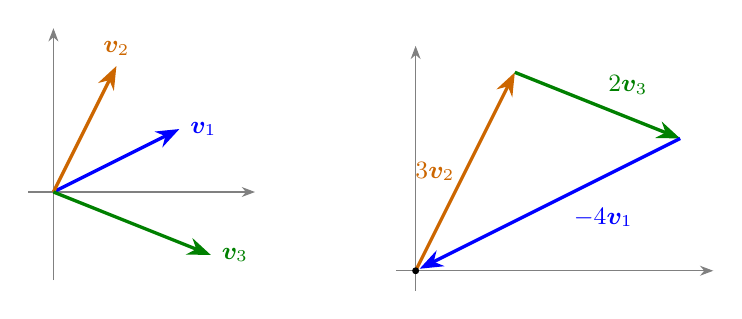
\begin{tikzpicture}[>=Stealth]
  \begin{scope}[scale=0.8]
    \draw[->,gray] (-0.4,0) -- (3.2,0);
    \draw[->,gray] (0,-1.4) -- (0,2.6);
    \draw[->,very thick,blue] (0,0) -- (2,1) node[right,font=\small] {$\vb{v}_1$};
    \draw[->,very thick,orange!80!black] (0,0) -- (1,2) node[above,font=\small] {$\vb{v}_2$};
    \draw[->,very thick,green!50!black] (0,0) -- (2.5,-1) node[right,font=\small] {$\vb{v}_3$};
  \end{scope}
  \begin{scope}[xshift=4.6cm,yshift=-1.0cm,scale=0.42]
    \draw[->,gray] (-0.6,0) -- (9,0);
    \draw[->,gray] (0,-0.6) -- (0,6.8);
    \draw[->,very thick,orange!80!black] (0,0) -- (3,6) node[midway,left,font=\small] {$3\vb{v}_2$};
    \draw[->,very thick,green!50!black] (3,6) -- (8,4) node[midway,above right,font=\small] {$2\vb{v}_3$};
    \draw[->,very thick,blue] (8,4) -- (0.12,0.06) node[pos=0.45,below right,font=\small] {$-4\vb{v}_1$};
    \fill (0,0) circle (3pt);
  \end{scope}
\end{tikzpicture}
\caption{Left: three vectors in $\R^2$. Right: the combination $3\vb{v}_2+2\vb{v}_3-4\vb{v}_1$
traced head to tail returns to the origin, so the three vectors are dependent. Any three vectors in
the plane admit such a closed path (Corollary~\ref{cor:u10-toomany}).}
\label{fig:u10-loop}
\end{figure}

When the vectors are columns, independence is a statement about a nullspace, and elimination
decides it.

\begin{theorem}[Independence test]\label{thm:u10-test}
The columns of an $m\times n$ matrix $A$ are independent if and only if $\Nul{A}=\{\vb{0}\}$, if
and only if $\rank A=n$ (every column is a pivot column, no free variables).
\end{theorem}
\begin{proof}
$A\vb{c}=c_1\vb{a}_1+\dots+c_n\vb{a}_n$, so a combination of the columns that gives $\vb{0}$ is
exactly a vector $\vb{c}$ in $\Nul{A}$; the columns are independent precisely when the only such
vector is $\vb{c}=\vb{0}$. By Theorem~\ref{thm:u08-special}, $\Nul{A}=\{\vb{0}\}$ exactly when there
are no special solutions, i.e.\ no free columns, i.e.\ $r=n$.
\end{proof}

\begin{corollary}[Too many vectors]\label{cor:u10-toomany}
Any $n$ vectors in $\R^m$ with $n>m$ are dependent.
\end{corollary}
\begin{proof}
As columns of an $m\times n$ matrix they give $r\le m<n$, so Theorem~\ref{thm:u10-test} applies.
\end{proof}

\subsection{Spanning sets and bases}

\begin{definition}[Span]\label{def:u10-span}
Vectors $\vb{v}_1,\dots,\vb{v}_k$ \emph{span} a space $V$ if $V$ consists of all their linear
combinations; we write $V=\Span\{\vb{v}_1,\dots,\vb{v}_k\}$. For example, the columns of $A$ span
$\Col{A}$.
\end{definition}

The span is the \emph{smallest} subspace containing the vectors: it is a subspace (sums and multiples
of combinations are combinations), and any subspace that contains $\vb{v}_1,\dots,\vb{v}_k$ must
contain all their combinations.

\begin{definition}[Basis]\label{def:u10-basis}
A \emph{basis} for a vector space $V$ is a list of vectors $\vb{v}_1,\dots,\vb{v}_d$ that (i) are
independent and (ii) span $V$.
\end{definition}

Spanning means there are enough vectors; independence means there are not too many. A basis tells
us everything about the space: every vector in it is a combination of the basis vectors, and, by the
next proposition, in only one way.

\begin{proposition}[Coordinates are unique]\label{prop:u10-unique}
If $\vb{v}_1,\dots,\vb{v}_d$ is a basis of $V$, every $\vb{v}\in V$ can be written as
$\vb{v}=c_1\vb{v}_1+\dots+c_d\vb{v}_d$ in exactly one way.
\end{proposition}
\begin{proof}
Spanning gives at least one way. If $\sum c_i\vb{v}_i=\sum c_i'\vb{v}_i$ then
$\sum(c_i-c_i')\vb{v}_i=\vb{0}$, and independence forces $c_i=c_i'$ for every $i$.
\end{proof}

\begin{proposition}[Bases of \texorpdfstring{\(\R^n\)}{Rn}]\label{prop:u10-Rn}
Vectors $\vb{v}_1,\dots,\vb{v}_n$ in $\R^n$ form a basis of $\R^n$ if and only if the $n\times n$
matrix with these columns is invertible.
\end{proposition}
\begin{proof}
Let $A$ be that matrix. Independence means $r=n$ (Theorem~\ref{thm:u10-test}); spanning $\R^n$ means
$A\vb{x}=\vb{b}$ is solvable for every $\vb{b}$, i.e.\ $r=m=n$ (Theorem~\ref{thm:u09-fullrank}).
For a square matrix both say $r=n$, which is invertibility.
\end{proof}

\begin{example}[Many bases of \texorpdfstring{\(\R^3\)}{R3}]\label{ex:u10-R3}
The standard basis $(1,0,0),(0,1,0),(0,0,1)$ consists of the columns of $I$, and
$\Nul{I}=\{\vb{0}\}$. It is far from the only basis. The vectors $(1,1,2)$ and $(2,2,5)$ are
independent (neither is a multiple of the other) but cannot span $\R^3$: as columns of a $3\times2$
matrix they give $r\le2<3$. They \emph{are} a basis for the plane they span. To complete them to a
basis of $\R^3$ we need a third vector outside that plane. $(3,3,7)$ fails, being their sum. The
vector $(1,0,0)$ works: the matrix $\begin{bmatrix}1&2&1\\1&2&0\\2&5&0\end{bmatrix}$ is invertible
(its determinant is $1$; elimination finds three pivots).
\end{example}

\begin{trap}
In the lecture, after rejecting $(3,3,7)$, the vector $(3,3,8)$ was offered as a third basis vector
``sticking a little out of the plane''. It does not: the matrix
$\begin{bmatrix}1&2&3\\1&2&3\\2&5&8\end{bmatrix}$ has two equal rows, so it is not invertible and by
Proposition~\ref{prop:u10-Rn} its columns are dependent. Indeed $(3,3,8)=-(1,1,2)+2(2,2,5)$. Every
vector in the plane of $(1,1,2)$ and $(2,2,5)$ has equal first and second components, and so does
$(3,3,8)$. Checking the \emph{rows} can expose a dependence among the columns that is invisible
column by column; Section~\ref{sec:u11} explains why (row rank equals column rank).
\end{trap}

\subsection{Dimension}

All bases of $\R^3$ above had three vectors. That is the central fact of the section.

\begin{lemma}[Independent sets are no larger than spanning sets]\label{lem:u10-count}
If $\vb{v}_1,\dots,\vb{v}_m$ span $V$ and $\vb{w}_1,\dots,\vb{w}_n\in V$ are independent, then
$n\le m$.
\end{lemma}
\begin{proof}
Suppose $n>m$. Each $\vb{w}_j$ is a combination of the $\vb{v}$'s:
$\vb{w}_j=a_{1j}\vb{v}_1+\dots+a_{mj}\vb{v}_m$. Collect the coefficients in the $m\times n$ matrix
$A=(a_{ij})$; in matrix shorthand $W=VA$, where $V$ and $W$ have the $\vb{v}$'s and $\vb{w}$'s as
columns. Since $n>m$, Corollary~\ref{cor:u08-wide} gives $\vb{x}\neq\vb{0}$ with $A\vb{x}=\vb{0}$.
Then $W\vb{x}=VA\vb{x}=\vb{0}$, i.e.\ $x_1\vb{w}_1+\dots+x_n\vb{w}_n=\vb{0}$ with not all $x_j=0$,
contradicting the independence of the $\vb{w}$'s.
\end{proof}

\begin{theorem}[Every basis has the same size]\label{thm:u10-dim}
Any two bases of a vector space $V$ contain the same number of vectors.
\end{theorem}
\begin{proof}
Let $\vb{v}_1,\dots,\vb{v}_m$ and $\vb{w}_1,\dots,\vb{w}_n$ be bases. The $\vb{v}$'s span and the
$\vb{w}$'s are independent, so $n\le m$ by Lemma~\ref{lem:u10-count}. Exchanging roles,
$m\le n$.
\end{proof}

\begin{definition}[Dimension]\label{def:u10-dim}
The \emph{dimension} of $V$, written $\dim V$, is the number of vectors in any basis of $V$. The
space $\{\vb{0}\}$ has the empty basis and dimension $0$.
\end{definition}

So $\dim\R^n=n$, the plane spanned by $(1,1,2)$ and $(2,2,5)$ has dimension $2$, and a line through
the origin has dimension $1$. Knowing the dimension saves half the work of checking a basis:

\begin{proposition}[The right number of vectors]\label{prop:u10-right}
Let $\dim V=d$. (a) Any $d$ independent vectors in $V$ form a basis. (b) Any $d$ vectors that span
$V$ form a basis. (c) Any independent list in $V$ can be extended to a basis of $V$.
\end{proposition}
\begin{proof}
First a remark: if $\vb{u}_1,\dots,\vb{u}_k$ are independent and $\vb{u}\notin\Span\{\vb{u}_i\}$,
then $\vb{u}_1,\dots,\vb{u}_k,\vb{u}$ are independent. (In a combination equal to $\vb{0}$ the
coefficient of $\vb{u}$ must vanish, otherwise $\vb{u}$ would be a combination of the $\vb{u}_i$;
then the other coefficients vanish too.)

(c) Keep adjoining a vector of $V$ outside the current span. Each list stays independent, and by
Lemma~\ref{lem:u10-count} (comparing with a basis of $d$ vectors) no independent list has more than
$d$ vectors, so the process stops; when it stops the list spans $V$.
(a) If $d$ independent vectors did not span $V$, the remark would produce $d+1$ independent vectors,
contradicting Lemma~\ref{lem:u10-count}.
(b) If $d$ spanning vectors were dependent, one of them would be a combination of the others and
could be dropped, leaving $d-1$ spanning vectors; but a basis of $V$ consists of $d$ independent
vectors, contradicting Lemma~\ref{lem:u10-count}.
\end{proof}

\subsection{Bases for the column space and the nullspace}

\begin{example}[Pivot columns and special solutions]\label{ex:u10-CN}
Take
\[
A=\begin{bmatrix}1&2&3&1\\1&1&2&1\\1&2&3&1\end{bmatrix},\qquad
R=\begin{bmatrix}1&0&1&1\\0&1&1&0\\0&0&0&0\end{bmatrix}.
\]
The four columns span $\Col{A}$ by definition, but they are not independent: column~3 is
column~1 plus column~2, and column~4 equals column~1. The pivot columns $(1,1,1)$ and $(2,1,2)$
form a basis of $\Col{A}$, so $\dim\Col{A}=2=\rank A$. Other bases are columns $1,3$, or columns
$2,3$, or columns $2,4$, or vectors not among the columns at all such as $(2,2,2)$ and $(7,5,7)$
(two independent vectors in a two-dimensional space, Proposition~\ref{prop:u10-right}(a)). The
special solutions
\[
\vb{s}_1=(-1,-1,1,0),\qquad \vb{s}_2=(-1,0,0,1)
\]
record exactly those two dependencies, and they form a basis of $\Nul{A}$, which has dimension
$4-2=2$.
\end{example}

\begin{theorem}[Basis of the column space]\label{thm:u10-col}
The pivot columns of $A$ (columns of $A$ itself, not of $R$) form a basis of $\Col{A}$. Hence
$\dim\Col{A}=\rank A$.
\end{theorem}
\begin{proof}
Let $EA=R$ with $E$ invertible; by Proposition~\ref{prop:u08-same-null}, $A\vb{c}=\vb{0}$ if and
only if $R\vb{c}=\vb{0}$, so the columns of $A$ satisfy exactly the same linear relations as the
columns of $R$.

\emph{Independent:} a combination of the pivot columns of $A$ equal to $\vb{0}$ is a vector
$\vb{c}$ with $A\vb{c}=\vb{0}$ and nonzero entries only in pivot positions. Then $R\vb{c}=\vb{0}$.
The pivot columns of $R$ are the distinct identity columns $\vb{e}_1,\dots,\vb{e}_r$, so
$R\vb{c}=\sum_i c_{p_i}\vb{e}_i=\vb{0}$ forces every $c_{p_i}=0$.

\emph{Spanning:} for a free column $\vb{a}_j$, the special solution $\vb{s}_j$ has $1$ in position
$j$, zeros in the other free positions, and $A\vb{s}_j=\vb{0}$. So $\vb{a}_j$ equals minus a
combination of pivot columns. Every column, hence every vector of $\Col{A}$, is a combination of the
pivot columns.
\end{proof}

\begin{theorem}[Basis of the nullspace]\label{thm:u10-null}
The $n-r$ special solutions form a basis of $\Nul{A}$. Hence $\dim\Nul{A}=n-r$.
\end{theorem}
\begin{proof}
They span $\Nul{A}$ by Theorem~\ref{thm:u08-special}. If $\sum_j c_j\vb{s}_j=\vb{0}$, look at the
$j$th free position: only $\vb{s}_j$ is nonzero there, with entry $1$, so the left side has entry
$c_j$ there. Hence every $c_j=0$.
\end{proof}

Mind the grammar: a matrix has a rank, a space has a dimension. ``The rank of $A$ is the dimension
of its column space'' is correct; ``the dimension of $A$'' and ``the rank of $\Col{A}$'' are not.

\begin{example}[Basis and dimension of a span]\label{ex:u10-span}
Find a basis and the dimension of the subspace of $\R^5$ spanned by
\[
\vb{w}_1=(1,1,-2,0,-1),\ \ \vb{w}_2=(1,2,0,-4,1),\ \ \vb{w}_3=(0,1,3,-3,2),\ \ \vb{w}_4=(2,3,0,-2,0).
\]
\emph{As rows.} Put the vectors in the rows of a matrix and eliminate: row~2 $-$ row~1 and
row~4 $-\,2\,$row~1 give $(0,1,2,-4,2)$ and $(0,1,4,-2,2)$; subtracting this new row~2 from rows~3
and~4 gives $(0,0,1,1,0)$ and $(0,0,2,2,0)$; finally row~4 $-\,2\,$row~3 $=\vb{0}$. Every step
replaces a row by a combination of rows and can be undone, so the span of the rows never changes.
The three nonzero rows
\[
(1,1,-2,0,-1),\qquad(0,1,2,-4,2),\qquad(0,0,1,1,0)
\]
are independent (look at the staircase of leading entries) and span the space: a basis, and the
dimension is $3$.

\emph{As columns.} Put the vectors in the columns of a $5\times4$ matrix instead. Elimination
finds pivots in columns $1,2,3$, so $\vb{w}_1,\vb{w}_2,\vb{w}_3$ themselves form a basis
(Theorem~\ref{thm:u10-col}); the free column records $\vb{w}_4=3\vb{w}_1-\vb{w}_2+2\vb{w}_3$. Here
one must use the original columns: the columns of the eliminated matrix have zeros in their last two
entries and span a different space. Both answers are correct; a space has many bases but one
dimension.
\end{example}

\subsection{Exercises}

\begin{exercise}\label{exr:u10-six}
Find the largest possible number of independent vectors among
\begin{gather*}
\vb{v}_1=(1,-1,0,0),\ \vb{v}_2=(1,0,-1,0),\ \vb{v}_3=(1,0,0,-1),\\
\vb{v}_4=(0,1,-1,0),\ \vb{v}_5=(0,1,0,-1),\ \vb{v}_6=(0,0,1,-1).
\end{gather*}
\end{exercise}
\begin{solution}
Observe $\vb{v}_4=\vb{v}_2-\vb{v}_1$, $\vb{v}_5=\vb{v}_3-\vb{v}_1$ and $\vb{v}_6=\vb{v}_3-\vb{v}_2$,
so the span is that of $\vb{v}_1,\vb{v}_2,\vb{v}_3$. Eliminating
$\begin{bmatrix}\vb{v}_1&\vb{v}_2&\vb{v}_3\end{bmatrix}$ (row~2 $+$ row~1, then row~3 $+$ row~2,
then row~4 $+$ row~3) leaves pivots $1,1,1$ in the first three rows and a zero fourth row: three
pivots, so $\vb{v}_1,\vb{v}_2,\vb{v}_3$ are independent. The answer is $3$, the rank of the
$4\times6$ matrix of all six vectors. (All six vectors have components adding to zero, so they lie
in a three-dimensional subspace of $\R^4$; Section~\ref{sec:u13} meets them again as the edges of a
graph.)
\end{solution}

\begin{exercise}\label{exr:u10-plane}
Find a basis for the plane $x-2y+3z=0$ in $\R^3$, then a basis for its intersection with the
$xy$-plane, then a basis for all vectors perpendicular to the plane.
\end{exercise}
\begin{solution}
The plane is $\Nul{\begin{bmatrix}1&-2&3\end{bmatrix}}$. The pivot variable is $x$; the special
solutions are $\vb{v}_1=(2,1,0)$ (from $y=1,z=0$) and $\vb{v}_2=(-3,0,1)$ (from $y=0,z=1$), a basis
of the plane. The intersection with the $xy$-plane ($z=0$) contains $\vb{v}_1$ but not $\vb{v}_2$,
so it is a line, with basis $\vb{v}_1$. The vector $\vb{v}_3=(1,-2,3)$ satisfies
$\vb{v}_3\cdot\vb{v}_1=2-2+0=0$ and $\vb{v}_3\cdot\vb{v}_2=-3+0+3=0$, so it is perpendicular to the
plane; the perpendicular vectors form a line, with basis $\vb{v}_3$.
\end{solution}

\begin{exercise}\label{exr:u10-wdep}
Suppose $\vb{w}_1,\vb{w}_2,\vb{w}_3$ are independent. Show that $\vb{v}_1=\vb{w}_2-\vb{w}_3$,
$\vb{v}_2=\vb{w}_1-\vb{w}_3$, $\vb{v}_3=\vb{w}_1-\vb{w}_2$ are dependent, and that
$\vb{u}_1=\vb{w}_2+\vb{w}_3$, $\vb{u}_2=\vb{w}_1+\vb{w}_3$, $\vb{u}_3=\vb{w}_1+\vb{w}_2$ are
independent.
\end{exercise}
\begin{solution}
$\vb{v}_1-\vb{v}_2+\vb{v}_3=(\vb{w}_2-\vb{w}_3)-(\vb{w}_1-\vb{w}_3)+(\vb{w}_1-\vb{w}_2)=\vb{0}$ is a
nonzero combination giving $\vb{0}$. For the $\vb{u}$'s, suppose
$c_1\vb{u}_1+c_2\vb{u}_2+c_3\vb{u}_3=\vb{0}$, i.e.
$(c_2+c_3)\vb{w}_1+(c_1+c_3)\vb{w}_2+(c_1+c_2)\vb{w}_3=\vb{0}$. Independence of the $\vb{w}$'s gives
$c_2+c_3=c_1+c_3=c_1+c_2=0$; adding, $c_1+c_2+c_3=0$, and subtracting each equation gives
$c_1=c_2=c_3=0$.
\end{solution}

\begin{exercise}\label{exr:u10-invertible}
Let $\vb{v}_1,\dots,\vb{v}_n$ be a basis of $\R^n$ and $B$ an invertible $n\times n$ matrix. Show
that $B\vb{v}_1,\dots,B\vb{v}_n$ is also a basis of $\R^n$.
\end{exercise}
\begin{solution}
If $\sum c_iB\vb{v}_i=\vb{0}$ then $B\bigl(\sum c_i\vb{v}_i\bigr)=\vb{0}$; multiplying by $B^{-1}$
gives $\sum c_i\vb{v}_i=\vb{0}$, so all $c_i=0$. The $n$ vectors $B\vb{v}_i$ are therefore
independent, and since $\dim\R^n=n$, Proposition~\ref{prop:u10-right}(a) says they form a basis.
\end{solution}

% unit: u11
% sources: sources/099-the-four-fundamental-subspaces.txt, sources/157-the-four-fundamental-subspaces.txt, sources/158-mit18-06scf11-ses1-10sum-pdf-download-file.txt, sources/159-computing-the-four-fundamental-subspaces.txt, sources/160-mit18-06scf11-ses1-10prob-pdf-download-file.txt, sources/161-mit18-06scf11-ses1-10sol-pdf-download-file.txt
\section{The four fundamental subspaces}\label{sec:u11}

So far each matrix has come with two subspaces, the column space and the nullspace. Transposing
the matrix gives two more, and the four together are the heart of this approach to linear algebra.
This section finds a basis and the dimension of each, all from one elimination $EA=R$, and proves the
first great count: the row space and the column space have the same dimension $r$. That fact
already corrects the slip of Section~\ref{sec:u10}, where $(3,3,8)$ was proposed as independent of
$(1,1,2)$ and $(2,2,5)$: the matrix with those columns has two equal rows, so its row space is only
two-dimensional, and therefore so is its column space.

\subsection{Two subspaces in \texorpdfstring{\(\R^n\)}{Rn}, two in \texorpdfstring{\(\R^m\)}{Rm}}

\begin{definition}[The four fundamental subspaces]\label{def:u11-four}
Let $A$ be an $m\times n$ matrix.
\begin{itemize}
\item The \emph{column space} $\Col{A}\subseteq\R^m$: all combinations of the columns.
\item The \emph{nullspace} $\Nul{A}\subseteq\R^n$: all solutions of $A\vb{x}=\vb{0}$.
\item The \emph{row space} $\Col{A\T}\subseteq\R^n$: all combinations of the rows of $A$, written as
column vectors, i.e.\ the column space of $A\T$.
\item The \emph{left nullspace} $\Nul{A\T}\subseteq\R^m$: all solutions of $A\T\vb{y}=\vb{0}$.
\end{itemize}
\end{definition}

Transposing $A\T\vb{y}=\vb{0}$ gives $\vb{y}\T A=\vb{0}\T$: a row vector multiplying $A$ from the
\emph{left} gives the zero row. That explains the name. A vector $\vb{y}$ in the left nullspace lists
the coefficients of a combination of the rows of $A$ that produces the zero row, just as a vector in
$\Nul{A}$ lists a combination of the columns that produces the zero column. These are exactly the
vectors that appeared in the solvability test of Theorem~\ref{thm:u09-solvable}.
Figure~\ref{fig:u11-big} shows where the four spaces live.

\begin{figure}[ht]\centering
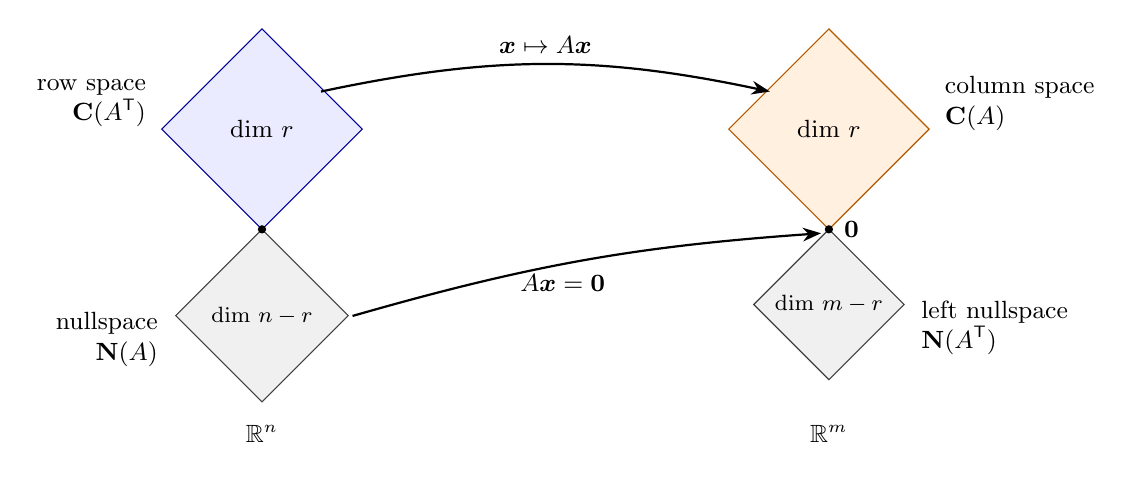
\begin{tikzpicture}[>=Stealth,font=\small]
  \begin{scope}
    \coordinate (On) at (0,0);
    \filldraw[fill=blue!8,draw=blue!60!black] (On) -- ++(45:1.8) -- ++(135:1.8) -- ++(225:1.8) -- cycle;
    \node at (0,1.27) {dim $r$};
    \node[anchor=east,align=right] at (-1.35,1.6) {row space\\$\Col{A\T}$};
    \filldraw[fill=gray!12,draw=gray!50!black] (On) -- ++(-45:1.55) -- ++(-135:1.55) -- ++(135:1.55) -- cycle;
    \node[font=\footnotesize] at (0,-1.1) {dim $n-r$};
    \node[anchor=east,align=right] at (-1.2,-1.4) {nullspace\\$\Nul{A}$};
    \fill (On) circle (1.5pt);
    \node at (0,-2.6) {$\R^n$};
  \end{scope}
  \begin{scope}[xshift=7.2cm]
    \coordinate (Om) at (0,0);
    \filldraw[fill=orange!12,draw=orange!70!black] (Om) -- ++(45:1.8) -- ++(135:1.8) -- ++(225:1.8) -- cycle;
    \node at (0,1.27) {dim $r$};
    \node[anchor=west,align=left] at (1.35,1.6) {column space\\$\Col{A}$};
    \filldraw[fill=gray!12,draw=gray!50!black] (Om) -- ++(-45:1.35) -- ++(-135:1.35) -- ++(135:1.35) -- cycle;
    \node[font=\footnotesize] at (0,-0.95) {dim $m-r$};
    \node[anchor=west,align=left] at (1.05,-1.25) {left nullspace\\$\Nul{A\T}$};
    \fill (Om) circle (1.5pt) node[right=2pt] {$\vb{0}$};
    \node at (0,-2.6) {$\R^m$};
  \end{scope}
  \draw[->,thick] (0.75,1.75) to[bend left=12] node[above] {$\vb{x}\mapsto A\vb{x}$} (6.45,1.75);
  \draw[->,thick] (1.15,-1.1) to[bend left=6] node[below,pos=0.45] {$A\vb{x}=\vb{0}$} (7.1,-0.05);
\end{tikzpicture}
\caption{The four fundamental subspaces of an $m\times n$ matrix of rank $r$. The row space and
nullspace live in $\R^n$ and their dimensions add to $n$; the column space and left nullspace live
in $\R^m$ and their dimensions add to $m$. $A$ sends every input into the column space and sends the
nullspace to $\vb{0}$.}
\label{fig:u11-big}
\end{figure}

For the column space and the nullspace the work is already done (Theorems~\ref{thm:u10-col}
and~\ref{thm:u10-null}): the pivot columns of $A$ are a basis of $\Col{A}$, of dimension $r$, and
the $n-r$ special solutions are a basis of $\Nul{A}$. One could treat $A\T$ the same way, but that
means a second elimination. The point is that the elimination already done on $A$ suffices.

\subsection{The row space}

\begin{theorem}[Row space]\label{thm:u11-row}
If $E$ is invertible and $EA=R$, then $A$ and $R$ have the same row space. In particular the $r$
nonzero rows of $R=\operatorname{rref}(A)$ form a basis of $\Col{A\T}$, and $\dim\Col{A\T}=r$.
\end{theorem}
\begin{proof}
Row $i$ of $R=EA$ is $\sum_k e_{ik}(\text{row }k\text{ of }A)$, a combination of the rows of $A$;
so the row space of $R$ is contained in that of $A$. Since $A=E^{-1}R$, each row of $A$ is likewise a
combination of the rows of $R$, giving the reverse inclusion. The zero rows of $R$ contribute
nothing, so the $r$ nonzero rows span. They are independent: the $i$th nonzero row has a $1$ in the
$i$th pivot column, where every other row of $R$ has a $0$, so in any combination equal to
$\vb{0}$ the $i$th coefficient is $0$.
\end{proof}

\begin{corollary}[Row rank equals column rank]\label{cor:u11-rankT}
For every matrix, $\dim\Col{A\T}=\dim\Col{A}$; that is, $\rank A\T=\rank A$.
\end{corollary}
\begin{proof}
Both dimensions equal the number $r$ of pivots of $A$, by Theorems~\ref{thm:u11-row}
and~\ref{thm:u10-col}. Applying Theorem~\ref{thm:u10-col} to $A\T$ shows that $\dim\Col{A\T}$ is
also the rank of $A\T$.
\end{proof}

This is a statement with content: there is no evident reason why the number of independent rows of
a $3\times 7$ matrix should equal its number of independent columns, yet it always does.

\subsection{The left nullspace and the matrix \texorpdfstring{\(E\)}{E}}

To find $\Nul{A\T}$ without transposing, we keep a record of the elimination. Attach the $m\times m$
identity to $A$ and apply to $\begin{bmatrix}A&I\end{bmatrix}$ the row operations that turn $A$
into $R$:
\[
\begin{bmatrix}A_{m\times n}&I_{m\times m}\end{bmatrix}\longrightarrow
\begin{bmatrix}R_{m\times n}&E_{m\times m}\end{bmatrix}.
\]
The row operations amount to multiplying on the left by some invertible matrix, and that matrix
turned $I$ into $E$, so it \emph{is} $E$: we get $EA=R$. When $A$ is square and invertible, $R=I$
and this is Gauss--Jordan: $E=A^{-1}$. In general $E$ is not unique when $r<m$ (one may add
multiples of the bottom rows to the others), but any such $E$ works below.

\begin{theorem}[Left nullspace]\label{thm:u11-left}
Let $EA=R$ with $E$ invertible and $R=\operatorname{rref}(A)$. The last $m-r$ rows of $E$ form a
basis of $\Nul{A\T}$, and $\dim\Nul{A\T}=m-r$.
\end{theorem}
\begin{proof}
$A\T$ is $n\times m$ with rank $r$ (Corollary~\ref{cor:u11-rankT}), so by
Theorem~\ref{thm:u10-null} its nullspace has dimension $m-r$. The last $m-r$ rows of $R=EA$ are
zero, so each of the last $m-r$ rows $\vb{y}\T$ of $E$ satisfies $\vb{y}\T A=\vb{0}\T$. These rows
are independent because $E$ is invertible (Theorem~\ref{thm:u10-test} applied to $E\T$). So they
are $m-r$ independent vectors in an $(m-r)$-dimensional space, and Proposition~\ref{prop:u10-right}(a)
makes them a basis.
\end{proof}

\begin{theorem}[Dimensions of the four subspaces]\label{thm:u11-dims}
For an $m\times n$ matrix of rank $r$:
\[
\dim\Col{A}=r,\qquad \dim\Nul{A}=n-r,\qquad \dim\Col{A\T}=r,\qquad \dim\Nul{A\T}=m-r.
\]
In $\R^n$: $r+(n-r)=n$. In $\R^m$: $r+(m-r)=m$.
\end{theorem}
\begin{proof}
Theorems~\ref{thm:u10-col}, \ref{thm:u10-null}, \ref{thm:u11-row} and~\ref{thm:u11-left}.
\end{proof}

The count $r+(n-r)=n$ is the old count of pivot variables plus free variables; the count in $\R^m$
is the same statement for $A\T$, which is just as good a matrix as $A$.

\begin{example}[All four subspaces at once]\label{ex:u11-four}
Take $A=\begin{bmatrix}1&2&3&1\\1&1&2&1\\1&2&3&1\end{bmatrix}$ from Example~\ref{ex:u10-CN},
so $m=3$, $n=4$, $r=2$. Reduce $\begin{bmatrix}A&I\end{bmatrix}$: subtract row~1 from rows~2 and~3,
multiply row~2 by $-1$, subtract $2\times$row~2 from row~1:
\[
\left[\begin{array}{cccc|ccc}1&2&3&1&1&0&0\\1&1&2&1&0&1&0\\1&2&3&1&0&0&1\end{array}\right]
\longrightarrow
\left[\begin{array}{cccc|ccc}1&0&1&1&-1&2&0\\0&1&1&0&1&-1&0\\0&0&0&0&-1&0&1\end{array}\right].
\]
Check $EA=R$ row by row: $-(1,2,3,1)+2(1,1,2,1)=(1,0,1,1)$, $(1,2,3,1)-(1,1,2,1)=(0,1,1,0)$,
$-(1,2,3,1)+(1,2,3,1)=\vb{0}$. Now read off:
\begin{itemize}
\item $\Col{A}$ (dimension $2$): pivot columns of $A$, $(1,1,1)$ and $(2,1,2)$.
\item $\Nul{A}$ (dimension $4-2=2$): special solutions $(-1,-1,1,0)$ and $(-1,0,0,1)$.
\item $\Col{A\T}$ (dimension $2$): nonzero rows of $R$, $(1,0,1,1)$ and $(0,1,1,0)$.
\item $\Nul{A\T}$ (dimension $3-2=1$): last row of $E$, $\vb{y}=(-1,0,1)$; indeed
$-(\text{row }1)+(\text{row }3)$ is the zero row.
\end{itemize}
\end{example}

\begin{trap}
Elimination keeps the row space and the nullspace but changes the column space and the left
nullspace. In Example~\ref{ex:u11-four}, $(1,1,1)$ is a column of $A$, so it lies in $\Col{A}$;
but every column of $R$ has third component $0$, so $(1,1,1)\notin\Col{R}$. Take the
\emph{rows of $R$} for the row space, but the \emph{columns of $A$} for the column space. Likewise
$\Nul{R\T}$ is spanned by $(0,0,1)$, not by the correct $(-1,0,1)$.
\end{trap}

\subsection{What a matrix keeps and what it crushes}

\begin{example}[The four subspaces of a rank-one matrix]\label{ex:u11-crush}
Return to $A=\begin{bmatrix}1&2&2\\2&4&4\end{bmatrix}$ from Example~\ref{ex:u08-crush}, with
$m=2$, $n=3$ and $r=1$.
\begin{itemize}
\item \emph{Inputs, $\R^3$.} The row space is the line through $(1,2,2)$ (dimension $r=1$). The
nullspace is the plane spanned by $\vb{s}_1=(-2,1,0)$ and $\vb{s}_2=(-2,0,1)$ (dimension
$n-r=2$). Both special solutions are perpendicular to $(1,2,2)$. Count: $1+2=3$.
\item \emph{Outputs, $\R^2$.} Every column is a multiple of $(1,2)$, so the column space is the
line through $(1,2)$ (dimension $1$). Row~2 minus $2\times$row~1 is zero, so $\vb{y}=(-2,1)$, or
equally $(2,-1)$, spans the left nullspace (dimension $m-r=1$). Count: $1+1=2$.
\end{itemize}
Now take the input $\vb{x}=(-1,3,2)$. It splits as a row-space part plus a nullspace part,
\[
\vb{x}=\begin{bmatrix}-1\\3\\2\end{bmatrix}=\begin{bmatrix}1\\2\\2\end{bmatrix}+\begin{bmatrix}-2\\1\\0\end{bmatrix},
\qquad
A\vb{x}=\begin{bmatrix}-1+6+4\\-2+12+8\end{bmatrix}=\begin{bmatrix}9\\18\end{bmatrix}
=A\begin{bmatrix}1\\2\\2\end{bmatrix}.
\]
The nullspace part was crushed to $\vb{0}$; only the row-space part reached the output, landing at
$(9,18)$ on the column-space line. The information that $A$ destroys is not scattered at random:
it is exactly the nullspace component, and that subspace is perpendicular to the rows.
(Section~\ref{sec:u16} proves that the nullspace is always perpendicular to the row space, and the
left nullspace to the column space; here $(1,2)\cdot(2,-1)=0$.) Figure~\ref{fig:u11-crush}
draws both sides.
\end{example}

\begin{figure}[ht]\centering
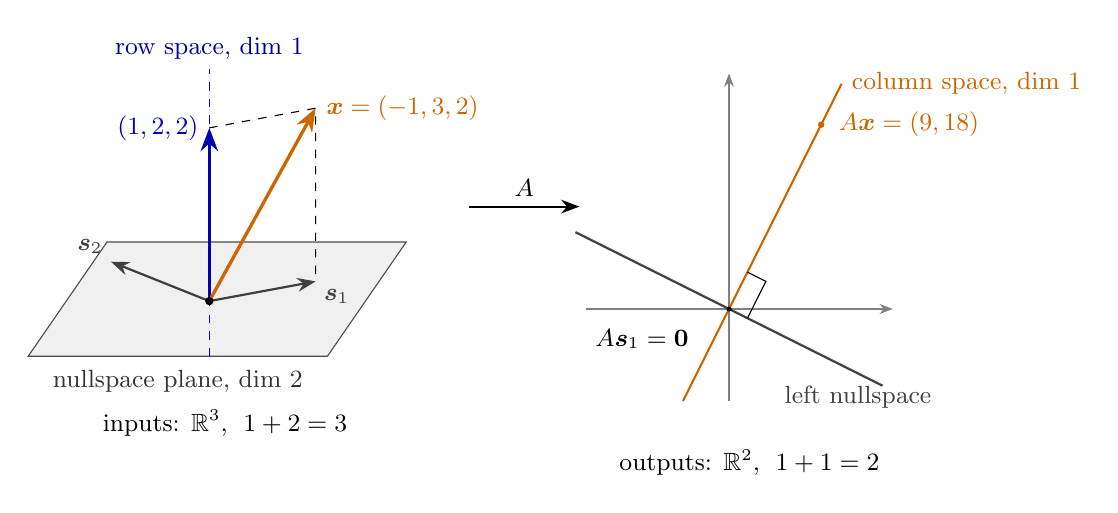
\begin{tikzpicture}[>=Stealth,font=\small]
  % input space R^3 (schematic): nullspace plane as a floor, row space as the vertical line
  \begin{scope}
    \fill[gray!12] (-2.3,-0.9) -- (1.5,-0.9) -- (2.5,0.55) -- (-1.3,0.55) -- cycle;
    \draw[gray!60!black] (-2.3,-0.9) -- (1.5,-0.9) -- (2.5,0.55) -- (-1.3,0.55) -- cycle;
    \node[gray!40!black,anchor=north] at (-0.4,-0.95) {nullspace plane, dim 2};
    \coordinate (O) at (0,-0.2);
    \draw[blue!60!black,dashed] (0,-0.9) -- (0,2.75);
    \node[blue!60!black,anchor=south] at (0,2.75) {row space, dim 1};
    \draw[->,thick,gray!50!black] (O) -- (1.35,0.05) node[below right=-1pt] {$\vb{s}_1$};
    \draw[->,thick,gray!50!black] (O) -- (-1.25,0.3) node[above left=-1pt] {$\vb{s}_2$};
    \draw[->,very thick,blue!70!black] (O) -- (0,2.0) node[left] {$(1,2,2)$};
    \draw[dashed] (0,2.0) -- (1.35,2.25) -- (1.35,0.05);
    \draw[->,very thick,orange!80!black] (O) -- (1.35,2.25) node[right] {$\vb{x}=(-1,3,2)$};
    \fill (O) circle (1.5pt);
    \node at (0.2,-1.75) {inputs: $\R^3$, \;$1+2=3$};
  \end{scope}
  % map
  \draw[->,thick] (3.3,1.0) -- node[above] {$A$} (4.7,1.0);
  % output space R^2, true proportions (scale 0.13)
  \begin{scope}[xshift=6.6cm,yshift=-0.3cm,scale=0.13]
    \draw[->,gray] (-14,0) -- (16,0);
    \draw[->,gray] (0,-9) -- (0,23);
    \draw[orange!80!black,thick] (-4.5,-9) -- (11,22) node[right] {column space, dim 1};
    \draw[gray!50!black,thick] (-15,7.5) -- (15,-7.5) node[below=1pt,pos=0.92] {left nullspace};
    \draw (1.8,3.6) -- (3.6,2.7) -- (1.8,-0.9);
    \fill[orange!80!black] (9,18) circle (9pt) node[right=3pt] {$A\vb{x}=(9,18)$};
    \fill (0,0) circle (7pt);
    \node[anchor=north east] at (-3,-1) {$A\vb{s}_1=\vb{0}$};
    \node at (2,-15) {outputs: $\R^2$, \;$1+1=2$};
  \end{scope}
\end{tikzpicture}
\caption{The matrix $A=\begin{bmatrix}1&2&2\\2&4&4\end{bmatrix}$. Left (schematic): the input
$\vb{x}=(-1,3,2)$ is the row-space vector $(1,2,2)$ plus the nullspace vector $\vb{s}_1$.
Right (to scale): $A$ crushes $\vb{s}_1$ to $\vb{0}$ and sends the row-space part to
$(9,18)$ on the column-space line, which is perpendicular to the left nullspace line through
$(2,-1)$.}
\label{fig:u11-crush}
\end{figure}

\subsection{A new vector space: matrices}

Nothing in the definition of a vector space requires the vectors to be columns of numbers. All we
use is that vectors can be added and multiplied by scalars, following the usual rules.

\begin{example}[The space of \texorpdfstring{\(3\times3\)}{3 by 3} matrices]\label{ex:u11-M}
Let $M$ be the set of all $3\times3$ real matrices. Matrices can be added and multiplied by
numbers, there is a zero matrix, and all eight vector-space rules hold; that we can also
\emph{multiply} two matrices is irrelevant here. Three subspaces of $M$: all upper triangular
matrices $U$; all symmetric matrices $S$; and their intersection $S\cap U$, which is the set $D$ of
diagonal matrices (symmetric with zeros below the diagonal forces zeros above it). Each is closed
under addition and scalar multiplication. A basis of $D$ is
\[
\begin{bmatrix}1&0&0\\0&0&0\\0&0&0\end{bmatrix},\quad
\begin{bmatrix}0&0&0\\0&3&0\\0&0&0\end{bmatrix},\quad
\begin{bmatrix}0&0&0\\0&0&0\\0&0&7\end{bmatrix}:
\]
they are independent (a combination with weights $a,b,c$ is $\operatorname{diag}(a,3b,7c)$, which
is zero only when $a=b=c=0$), and every diagonal matrix $\operatorname{diag}(d_1,d_2,d_3)$ is the
combination with weights $d_1,\,d_2/3,\,d_3/7$. So $\dim D=3$. Section~\ref{sec:u12} finds the
dimensions of $M$, $S$ and $U$.
\end{example}

\subsection{Exercises}

\begin{exercise}\label{exr:u11-ineq}
$A$ is $m\times n$ of rank $r$, and some right-hand sides $\vb{b}$ give no solution of
$A\vb{x}=\vb{b}$. (a) Which inequalities ($<$ or $\le$) must hold between $m$, $n$ and $r$?
(b) How do you know that $A\T\vb{y}=\vb{0}$ has solutions other than $\vb{y}=\vb{0}$?
\end{exercise}
\begin{solution}
(a) Always $r\le m$ and $r\le n$. Since some $\vb{b}$ is unreachable, $\Col{A}\ne\R^m$, so
$r<m$ (Theorem~\ref{thm:u09-fullrank}(b)). Nothing more can be said about $r$ versus $n$.
(b) $\dim\Nul{A\T}=m-r>0$, so the left nullspace contains nonzero vectors.
\end{solution}

\begin{exercise}\label{exr:u11-ATy}
For which $\vb{d}$ is $A\T\vb{y}=\vb{d}$ solvable? When is the solution unique?
\end{exercise}
\begin{solution}
$A\T\vb{y}$ is a combination of the columns of $A\T$, i.e.\ of the rows of $A$, so the system is
solvable exactly when $\vb{d}$ is in the row space $\Col{A\T}$. Two solutions differ by a vector in
$\Nul{A\T}$, so the solution is unique when the left nullspace is $\{\vb{0}\}$, i.e.\ when $r=m$.
\end{solution}

\begin{exercise}\label{exr:u11-LU}
Let $B=LU$ with $L=\begin{bmatrix}1&0&0\\2&1&0\\-1&0&1\end{bmatrix}$ and
$U=\begin{bmatrix}5&0&3\\0&1&1\\0&0&0\end{bmatrix}$. Find a basis and the dimension of each of the
four subspaces of $B$, without multiplying out $B$.
\end{exercise}
\begin{solution}
$U$ has two pivots, so $r=2$ and all four dimensions are $2$, $3-2=1$, $2$, $3-2=1$.
\emph{Column space:} since $L$ is invertible, the columns of $B=LU$ satisfy the same relations as
the columns of $U$, so columns~1 and~2 of $B$ are pivot columns. They are $L$ times $(5,0,0)$ and
$(0,1,0)$, i.e.\ $5(1,2,-1)$ and $(0,1,0)$; a basis is $(1,2,-1),(0,1,0)$, the first two columns
of $L$. \emph{Nullspace:} $\Nul{B}=\Nul{U}$; the free variable $x_3=1$ gives $x_2=-1$ and
$5x_1+3=0$, so the basis is $(-\tfrac35,-1,1)$. \emph{Row space:} $L^{-1}B=U$ is a sequence of row
operations, so the row space is spanned by the pivot rows of $U$: $(5,0,3)$ and $(0,1,1)$.
\emph{Left nullspace:} $L^{-1}=\begin{bmatrix}1&0&0\\-2&1&0\\1&0&1\end{bmatrix}$ plays the role of
$E$, and its last row $(1,0,1)$ is the basis: row~1 of $B$ is $(5,0,3)$, row~3 is $-(5,0,3)$, and
they cancel.
\end{solution}

\begin{exercise}\label{exr:u11-construct}
Find a $3\times3$ matrix whose column space contains $(1,1,0)$ and $(1,0,1)$ and whose nullspace
contains $(1,1,1)$. What must its rank be?
\end{exercise}
\begin{solution}
The column space contains two independent vectors, so $r\ge2$; the nullspace is at least a line,
so $3-r\ge1$. Hence $r=2$. The condition $A(1,1,1)=\vb{0}$ says the three columns add to zero. Take
the first two columns to be the given vectors and the third their negative sum:
$A=\begin{bmatrix}1&1&-2\\1&0&-1\\0&1&-1\end{bmatrix}$. Its column space is the plane spanned by
$(1,1,0)$ and $(1,0,1)$, and $A(1,1,1)=(0,0,0)$.
\end{solution}

% unit: u12
% sources: sources/070-matrix-spaces-rank-1-small-world-graphs.txt, sources/162-matrix-spaces-rank-1-small-world-graphs.txt, sources/163-mit18-06scf11-ses1-11sum-pdf-download-file.txt, sources/164-matrix-spaces.txt, sources/165-mit18-06scf11-ses1-11prob-pdf-download-file.txt, sources/166-mit18-06scf11-ses1-11sol-pdf-download-file.txt
\section{Matrix spaces; rank one; small world graphs}\label{sec:u12}

Everything in Sections~\ref{sec:u10} and~\ref{sec:u11} used only two operations: adding vectors and
multiplying them by numbers. So the same ideas (subspace, basis, dimension) apply to any objects
that can be added and scaled. This section works them out for spaces of matrices and a space of
functions, introduces two natural operations on subspaces (intersection and sum), shows that
rank-one matrices are the building blocks of every matrix, and ends with the graphs that lead into
Section~\ref{sec:u13}.

\subsection{Bases and dimensions of matrix spaces}

Let $M$ be the space of all $3\times3$ matrices (Example~\ref{ex:u11-M}). Write $E_{ij}$ for the
matrix with a $1$ in position $(i,j)$ and zeros elsewhere.

\begin{proposition}[Dimensions in \texorpdfstring{\(M\)}{M}]\label{prop:u12-dims}
\begin{enumerate}[(a)]
\item The nine matrices $E_{ij}$ form a basis of $M$, so $\dim M=9$.
\item The six $E_{ij}$ with $i\le j$ form a basis of the upper triangular matrices $U$: $\dim U=6$.
\item $E_{11},E_{22},E_{33},\ E_{12}+E_{21},\ E_{13}+E_{31},\ E_{23}+E_{32}$ form a basis of the
symmetric matrices $S$: $\dim S=6$.
\item $E_{11},E_{22},E_{33}$ form a basis of the diagonal matrices $D=S\cap U$: $\dim D=3$.
\end{enumerate}
\end{proposition}
\begin{proof}
(a) $A=\sum_{i,j}a_{ij}E_{ij}$, and this combination is the zero matrix only if every $a_{ij}=0$.
(b) The same argument applies to matrices with $a_{ij}=0$ for $i>j$. (c) A symmetric matrix is
determined by its three diagonal entries and three entries above the diagonal:
$A=\sum_i a_{ii}E_{ii}+\sum_{i<j}a_{ij}(E_{ij}+E_{ji})$, and the six coefficients are entries of
$A$, so the combination vanishes only when they are all $0$. (d) As in (a).
\end{proof}

So $M$ is ``practically $\R^9$'', with the nine numbers written in a square. The bases of $U$ and
$D$ happen to be subsets of the standard basis of $M$; the basis of $S$ cannot be, because only three
of the nine $E_{ij}$ are symmetric. In general a subspace needs its own basis.

\subsection{Intersections and sums of subspaces}

\begin{proposition}[Intersection]\label{prop:u12-cap}
If $V$ and $W$ are subspaces of the same space, so is $V\cap W$.
\end{proposition}
\begin{proof}
If $\vb{x},\vb{y}$ lie in both $V$ and $W$, then $\vb{x}+\vb{y}$ and $c\vb{x}$ lie in $V$ (a
subspace) and in $W$ (a subspace).
\end{proof}

The union $V\cup W$ is usually \emph{not} a subspace: two different lines through the origin in
$\R^2$ are not closed under addition (Figure~\ref{fig:u12-sum}). To get a subspace we must fill in
between them.

\begin{definition}[Sum of subspaces]\label{def:u12-sum}
The \emph{sum} of subspaces $V$ and $W$ is $V+W=\{\vb{v}+\vb{w}:\vb{v}\in V,\ \vb{w}\in W\}$.
\end{definition}

$V+W$ is a subspace: $(\vb{v}+\vb{w})+(\vb{v}'+\vb{w}')=(\vb{v}+\vb{v}')+(\vb{w}+\vb{w}')$ and
$c(\vb{v}+\vb{w})=c\vb{v}+c\vb{w}$. It is the smallest subspace containing $V\cup W$, since any
subspace containing both must contain all such sums.

\begin{figure}[ht]\centering
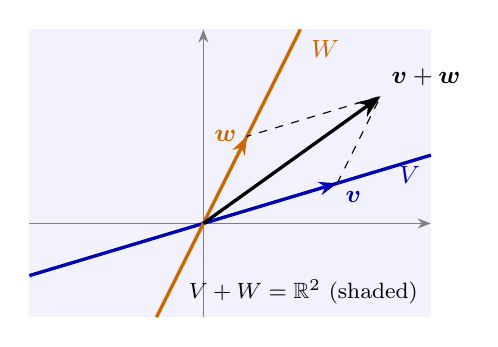
\begin{tikzpicture}[scale=0.85,>=Stealth,font=\small]
  \fill[blue!5] (-2.6,-1.4) rectangle (3.4,2.9);
  \draw[->,gray] (-2.6,0) -- (3.4,0);
  \draw[->,gray] (0,-1.4) -- (0,2.9);
  \draw[very thick,blue!70!black] (-2.6,-0.78) -- (3.4,1.02) node[below left] {$V$};
  \draw[very thick,orange!80!black] (-0.7,-1.4) -- (1.45,2.9) node[below right] {$W$};
  \draw[->,thick,blue!70!black] (0,0) -- (2,0.6) node[below right=-1pt] {$\vb{v}$};
  \draw[->,thick,orange!80!black] (0,0) -- (0.65,1.3) node[left] {$\vb{w}$};
  \draw[dashed] (2,0.6) -- (2.65,1.9) -- (0.65,1.3);
  \draw[->,very thick] (0,0) -- (2.65,1.9) node[above right] {$\vb{v}+\vb{w}$};
  \node[anchor=south east,align=right,font=\footnotesize] at (3.35,-1.35) {$V+W=\R^2$ (shaded)};
\end{tikzpicture}
\caption{Two lines $V$ and $W$ through the origin. Their union is not a subspace: $\vb{v}+\vb{w}$
lies on neither line. Their sum $V+W$ is the whole plane, and their intersection is $\{\vb{0}\}$,
so $\dim(V+W)+\dim(V\cap W)=2+0=1+1$.}
\label{fig:u12-sum}
\end{figure}

\begin{example}[Symmetric plus upper triangular]\label{ex:u12-SU}
$S+U=M$: every $3\times3$ matrix is a symmetric matrix plus an upper triangular one. Copy the part
below the diagonal into a symmetric matrix and put the rest into the upper triangular one:
\[
\begin{bmatrix}1&2&3\\4&5&6\\7&8&9\end{bmatrix}
=\begin{bmatrix}0&4&7\\4&0&8\\7&8&0\end{bmatrix}
+\begin{bmatrix}1&-2&-4\\0&5&-2\\0&0&9\end{bmatrix}.
\]
The same recipe works for every matrix. Note the dimensions: $\dim S+\dim U=6+6$ and
$\dim(S+U)+\dim(S\cap U)=9+3$.
\end{example}

\begin{theorem}[Dimension of a sum]\label{thm:u12-sumdim}
For finite-dimensional subspaces $V$ and $W$ of the same space,
\[
\dim(V+W)+\dim(V\cap W)=\dim V+\dim W.
\]
\end{theorem}
\begin{proof}
Let $\vb{u}_1,\dots,\vb{u}_k$ be a basis of $V\cap W$. By Proposition~\ref{prop:u10-right}(c)
it extends to a basis of $V$, say $\vb{u}_1,\dots,\vb{u}_k$, $\vb{v}_1,\dots,\vb{v}_p$, and to a
basis of $W$, say $\vb{u}_1,\dots,\vb{u}_k$, $\vb{w}_1,\dots,\vb{w}_q$. We claim that all $k+p+q$
vectors $\vb{u}_i,\vb{v}_j,\vb{w}_l$ together form a basis of $V+W$; then
$\dim(V+W)+\dim(V\cap W)=(k+p+q)+k=(k+p)+(k+q)$, as required.

They span $V+W$, since every $\vb{v}\in V$ and every $\vb{w}\in W$ is a combination of them. For
independence, suppose $\sum a_i\vb{u}_i+\sum b_j\vb{v}_j+\sum c_l\vb{w}_l=\vb{0}$. Then
$\vb{z}=\sum c_l\vb{w}_l=-\sum a_i\vb{u}_i-\sum b_j\vb{v}_j$ lies in $W$ (left side) and in $V$
(right side), hence in $V\cap W$, so $\vb{z}=\sum d_i\vb{u}_i$ for some $d_i$. Then
$\sum c_l\vb{w}_l-\sum d_i\vb{u}_i=\vb{0}$, and independence of the basis of $W$ gives all
$c_l=0$ (and $d_i=0$). Now $\sum a_i\vb{u}_i+\sum b_j\vb{v}_j=\vb{0}$, and independence of the
basis of $V$ gives all $a_i=b_j=0$.
\end{proof}

\begin{trap}
The dimension formula involves the \emph{sum} $V+W$, not the union. ``$\dim(S\cup U)$'' has no
meaning, because $S\cup U$ is not a vector space: the symmetric matrix $E_{12}+E_{21}$ plus the
upper triangular matrix $E_{12}$ is $2E_{12}+E_{21}$, which is neither symmetric nor upper
triangular.
\end{trap}

\subsection{A space of functions}

The solutions of the differential equation
\[
\frac{d^2y}{dx^2}+y=0
\]
form a vector space: if $y_1''+y_1=0$ and $y_2''+y_2=0$ then $(c_1y_1+c_2y_2)''+(c_1y_1+c_2y_2)=0$.
It is the ``nullspace'' of the operation $y\mapsto y''+y$. Both $\cos x$ and $\sin x$ are in it.

\begin{theorem}[Solutions of \texorpdfstring{\(y''+y=0\)}{y''+y=0}]\label{thm:u12-ode}
$\cos x$ and $\sin x$ form a basis of the solution space, which therefore has dimension $2$. The
solution with $y(0)=a$ and $y'(0)=b$ is $y=a\cos x+b\sin x$.
\end{theorem}
\begin{proof}
\emph{Independent:} if $c_1\cos x+c_2\sin x=0$ for all $x$, then $x=0$ gives $c_1=0$ and
$x=\pi/2$ gives $c_2=0$.
\emph{Spanning:} let $y$ be any solution and put $z=y-y(0)\cos x-y'(0)\sin x$. Then $z$ is a
solution with $z(0)=0$ and $z'(0)=0$. The quantity $E=z^2+(z')^2$ satisfies
$E'=2zz'+2z'z''=2z'(z+z'')=0$, so $E$ is constant, equal to $E(0)=0$. Hence $z\equiv0$ and
$y=y(0)\cos x+y'(0)\sin x$.
\end{proof}

These two functions play the role of the special solutions: a second-order equation has a
two-dimensional solution space, and solving it means finding a basis. Other bases exist; if complex
scalars are allowed, $e^{ix}$ and $e^{-ix}$ form one (they are $\cos x\pm i\sin x$). For example,
the solution with $y(0)=2$ and $y'(0)=-1$ is $y=2\cos x-\sin x$; check:
$y''=-2\cos x+\sin x=-y$.

\subsection{Rank-one matrices}

\begin{example}[A column times a row]\label{ex:u12-rank1}
In $A=\begin{bmatrix}1&4&5\\2&8&10\end{bmatrix}$ the second row is twice the first, so the rank is
$1$. A basis of the row space is $(1,4,5)$, a basis of the column space is $(1,2)$, and every column
is a multiple of $(1,2)$, with multipliers $1,4,5$. That is exactly the product
\[
A=\begin{bmatrix}1\\2\end{bmatrix}\begin{bmatrix}1&4&5\end{bmatrix}.
\]
\end{example}

\begin{theorem}[Rank one]\label{thm:u12-rank1}
A matrix has rank $1$ if and only if it equals $\vb{u}\vb{v}\T$ for some nonzero column vectors
$\vb{u}\in\R^m$, $\vb{v}\in\R^n$. Then $\Col{A}$ is the line through $\vb{u}$, $\Col{A\T}$ is the
line through $\vb{v}$, and $\Nul{A}=\{\vb{x}:\vb{v}\T\vb{x}=0\}$.
\end{theorem}
\begin{proof}
Column $j$ of $\vb{u}\vb{v}\T$ is $v_j\vb{u}$, so every column lies on the line through $\vb{u}$,
and some column is nonzero because $\vb{v}\ne\vb{0}$ and $\vb{u}\ne\vb{0}$; hence the column space
is that line and the rank is $1$. Conversely, if $\rank A=1$, then $\Col{A}$ has a basis consisting
of one vector $\vb{u}$, so each column is $\vb{a}_j=v_j\vb{u}$ for some number $v_j$; that says
$A=\vb{u}\vb{v}\T$, and $\vb{v}\ne\vb{0}$ because $A\ne0$. The same argument applied to the rows
($A\T=\vb{v}\vb{u}\T$) gives the row space. Finally
$A\vb{x}=\vb{u}(\vb{v}\T\vb{x})=\vb{0}$ exactly when the number $\vb{v}\T\vb{x}$ is $0$.
\end{proof}

\begin{example}[The four subspaces of \texorpdfstring{\(\begin{bmatrix}1&1&1&1\end{bmatrix}\)}{[1 1 1 1]}]\label{ex:u12-sum0}
The vectors $\vb{v}\in\R^4$ with $v_1+v_2+v_3+v_4=0$ form a subspace, the nullspace of the
rank-one matrix $A=\begin{bmatrix}1&1&1&1\end{bmatrix}$ ($m=1$, $n=4$, $r=1$). The pivot variable
is $v_1$, and the three special solutions
\[
(-1,1,0,0),\qquad(-1,0,1,0),\qquad(-1,0,0,1)
\]
are a basis, so the dimension is $n-r=3$. The row space is the line through $(1,1,1,1)$
(dimension~1); $3+1=4$. The column space is all of $\R^1$ (dimension $1$), and the left nullspace is
$\{0\}$ (dimension $0$, with the empty set as basis); $1+0=1$.
\end{example}

Rank-one matrices are the building blocks of all matrices.

\begin{theorem}[A sum of rank-one pieces]\label{thm:u12-CR}
Let $A$ have rank $r$, let $C$ be the $m\times r$ matrix of pivot columns of $A$, and let $R_0$ be
the $r\times n$ matrix of nonzero rows of $R=\operatorname{rref}(A)$. Then $A=CR_0$; equivalently, $A$
is the sum of the $r$ rank-one matrices $(\text{pivot column }k)(\text{row }k\text{ of }R_0)$.
\end{theorem}
\begin{proof}
Column $j$ of $CR_0$ is $C$ times column $j$ of $R_0$. If $j$ is the $k$th pivot column, column $j$
of $R_0$ is the $k$th standard basis vector and the product is the $k$th column of $C$, which is
$\vb{a}_j$. If $j$ is free, column $j$ of $R_0$ holds the entries $f_{1j},\dots,f_{rj}$ of $F$ in
that column, and the special solution $\vb{s}_j$ (pivot entries $-f_{kj}$, entry $1$ in position $j$)
gives $A\vb{s}_j=\vb{a}_j-\sum_kf_{kj}(\text{pivot column }k)=\vb{0}$. So
$\vb{a}_j=\sum_kf_{kj}(\text{pivot column }k)$, which is again column $j$ of $CR_0$. The column-row
expansion of a product then writes $CR_0$ as a sum of $r$ column-times-row terms.
\end{proof}

For the matrix of Example~\ref{ex:u11-four} this reads
\[
\begin{bmatrix}1&2&3&1\\1&1&2&1\\1&2&3&1\end{bmatrix}
=\begin{bmatrix}1\\1\\1\end{bmatrix}\begin{bmatrix}1&0&1&1\end{bmatrix}
+\begin{bmatrix}2\\1\\2\end{bmatrix}\begin{bmatrix}0&1&1&0\end{bmatrix},
\]
two rank-one pieces for a rank-two matrix. In the same way a $5\times17$ matrix of rank $4$ is a sum
of four rank-one matrices.

\begin{proposition}[Rank of a sum]\label{prop:u12-subadd}
$\rank(A+B)\le\rank A+\rank B$ for matrices of the same size.
\end{proposition}
\begin{proof}
Every column of $A+B$ is a column of $A$ plus a column of $B$, so $\Col{A+B}\subseteq\Col{A}+\Col{B}$.
By Theorem~\ref{thm:u12-sumdim}, $\dim(\Col{A}+\Col{B})\le\dim\Col{A}+\dim\Col{B}$.
\end{proof}

Consequently the rank-one matrices do \emph{not} form a subspace of $M$: $E_{11}+E_{22}$ has rank $2$.
Nor do the $5\times17$ matrices of rank at most $4$ (even with the zero matrix included): with
$E_{ij}$ now $5\times17$, the matrices $E_{11}+E_{22}+E_{33}+E_{44}$ and
$E_{22}+E_{33}+E_{44}+E_{55}$ have rank $4$, but their sum has the five pivots $1,2,2,2,1$ and rank
$5$.

\subsection{Small world graphs}

\begin{definition}[Graph, distance, diameter]\label{def:u12-graph}
A \emph{graph} $G=\{\text{nodes},\text{edges}\}$ is a set of nodes together with edges, each edge
joining two nodes. The \emph{distance} between two nodes is the smallest number of edges in a path
joining them; the \emph{diameter} is the largest distance between two nodes.
\end{definition}

Take one node for each person in a country and an edge between any two people who are friends. The
phrase ``six degrees of separation'' is the claim that this graph has small diameter, roughly six;
when two strangers on a plane find a mutual friend they remark that it is a small world. The World
Wide Web, with sites as nodes and links as edges, raises the same question. The mathematical point
is that a few long-range shortcuts make all distances drop dramatically.

\begin{example}[A ring with shortcuts]\label{ex:u12-ring}
Put $12$ people in a ring, each friends only with the two neighbours. The distance between nodes
$i$ and $j$ is $\min(|i-j|,\,12-|i-j|)$, so the diameter is $6$. From any node the other eleven are
at distances $1,1,2,2,3,3,4,4,5,5,6$, which sum to $36$: the average distance is
$36/11\approx3.27$. Now add the long-range friendships $1$--$7$, $3$--$9$, $5$--$11$ one at a time
(Figure~\ref{fig:u12-ring}). Breadth-first search from every node gives
\begin{center}
\begin{tabular}{@{}lcccc@{}}
\toprule
shortcuts added & none & $1$--$7$ & $+\ 3$--$9$ & $+\ 5$--$11$\\
\midrule
diameter & $6$ & $6$ & $5$ & $3$\\
average distance & $3.27$ & $2.74$ & $2.39$ & $2.18$\\
\bottomrule
\end{tabular}
\end{center}
Three extra edges out of fifteen halve the diameter. For instance, after all three shortcuts node
$2$ reaches node $8$ in three steps ($2\to1\to7\to8$) instead of six.
\end{example}

\begin{figure}[ht]\centering
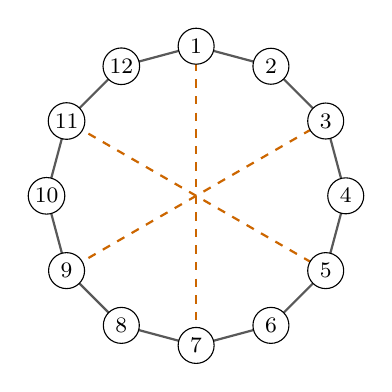
\begin{tikzpicture}[font=\footnotesize]
  \foreach \k in {1,...,12} {
    \coordinate (n\k) at ({90-30*(\k-1)}:1.9);
  }
  \foreach \k [evaluate=\k as \nxt using {int(mod(\k,12)+1)}] in {1,...,12} {
    \draw[thick,gray!70!black] (n\k) -- (n\nxt);
  }
  \draw[thick,dashed,orange!80!black] (n1) -- (n7);
  \draw[thick,dashed,orange!80!black] (n3) -- (n9);
  \draw[thick,dashed,orange!80!black] (n5) -- (n11);
  \foreach \k in {1,...,12} {
    \node[circle,draw,fill=white,inner sep=1.2pt,minimum size=13pt] at (n\k) {\k};
  }
\end{tikzpicture}
\caption{A ring of $12$ friends (solid) with three long-range shortcuts (dashed). Without shortcuts
the diameter is $6$; with them it is $3$.}
\label{fig:u12-ring}
\end{figure}

To study such questions with linear algebra we need a matrix for every graph. Section~\ref{sec:u13}
builds it, the incidence matrix, for a small directed graph.

\subsection{Exercises}

\begin{exercise}\label{exr:u12-perm}
Write the $3\times3$ identity as a combination of the other five $3\times3$ permutation matrices,
and show that those five are linearly independent. (They form a basis of the subspace of
$3\times3$ matrices whose row and column sums are all equal.)
\end{exercise}
\begin{solution}
The other five are $P_{21},P_{31},P_{32}$ (exchanging two rows of $I$) and the cyclic shifts
\[
P_{32}P_{21}=\begin{bmatrix}0&1&0\\0&0&1\\1&0&0\end{bmatrix},\qquad
P_{21}P_{32}=\begin{bmatrix}0&0&1\\1&0&0\\0&1&0\end{bmatrix}.
\]
$P_{21}+P_{31}+P_{32}$ is the all-ones matrix and $P_{32}P_{21}+P_{21}P_{32}$ has zeros on the diagonal
and ones elsewhere, so $I=P_{21}+P_{31}+P_{32}-P_{32}P_{21}-P_{21}P_{32}$. For independence,
\[
c_1P_{21}+c_2P_{31}+c_3P_{32}+c_4P_{32}P_{21}+c_5P_{21}P_{32}=
\begin{bmatrix}c_3&c_1+c_4&c_2+c_5\\c_1+c_5&c_2&c_3+c_4\\c_2+c_4&c_3+c_5&c_1\end{bmatrix}.
\]
If this is zero, the diagonal gives $c_1=c_2=c_3=0$ and then the off-diagonal entries give
$c_4=c_5=0$.
\end{solution}

\begin{exercise}\label{exr:u12-AX}
Let $M$ be the space of $3\times3$ matrices and $A=\begin{bmatrix}1&0&-1\\-1&1&0\\0&-1&1\end{bmatrix}$.
Consider the operation $X\mapsto AX$ on $M$. (a) Which $X$ give $AX=0$? (b) Which matrices have
the form $AX$? (c) What are the dimensions of these two subspaces of $M$, and why do they add to $9$?
\end{exercise}
\begin{solution}
(a) $A$ has rank $2$ (the rows add to zero, and the first two are independent), and
$\Nul{A}$ is the line through $(1,1,1)$. $AX=0$ means every column of $X$ lies in $\Nul{A}$, so
$X=\begin{bmatrix}a&b&c\\a&b&c\\a&b&c\end{bmatrix}$. (b) The columns of $AX$ are combinations of the
columns of $A$, all of which have components summing to $0$; and since $\Col{A}$ is the whole
plane of such vectors (dimension $2$), every matrix whose columns each sum to $0$ is some $AX$.
(c) The ``nullspace'' has dimension $3$ ($a,b,c$ free) and the ``column space'' has dimension $6$
(each of three columns lies in a $2$-dimensional plane). $3+6=9=\dim M$: the count
$(n-r)+r=n$ for an operation on a $9$-dimensional input space, column by column $1+2=3$.
\end{solution}

\begin{exercise}\label{exr:u12-211}
Show that the $2\times3$ matrices $A$ with $(2,1,1)$ in their nullspace form a subspace of the
space of $2\times3$ matrices, and find a basis and its dimension. Do the $2\times3$ matrices whose
column space contains $(2,1)$ form a subspace?
\end{exercise}
\begin{solution}
If $A(2,1,1)=\vb{0}$ and $B(2,1,1)=\vb{0}$ then $(A+B)(2,1,1)=\vb{0}$ and $(cA)(2,1,1)=\vb{0}$, so it
is a subspace. Each row $(a,b,c)$ must satisfy $2a+b+c=0$, i.e.\ $c=-2a-b$, so each row is a
combination of $(1,0,-2)$ and $(0,1,-1)$. A basis is
\[
\begin{bmatrix}1&0&-2\\0&0&0\end{bmatrix},\
\begin{bmatrix}0&1&-1\\0&0&0\end{bmatrix},\
\begin{bmatrix}0&0&0\\1&0&-2\end{bmatrix},\
\begin{bmatrix}0&0&0\\0&1&-1\end{bmatrix},
\]
and the dimension is $4$. The second set is not a subspace: the zero matrix has column space
$\{\vb{0}\}$, which does not contain $(2,1)$, yet every subspace contains the zero vector.
\end{solution}

\begin{exercise}\label{exr:u12-uvT}
Write $A=\begin{bmatrix}2&-4&6\\-1&2&-3\\3&-6&9\end{bmatrix}$ as $\vb{u}\vb{v}\T$, and give a basis
for each of its four subspaces.
\end{exercise}
\begin{solution}
Every row is a multiple of $(1,-2,3)$, with multipliers $2,-1,3$, so
$A=\vb{u}\vb{v}\T$ with $\vb{u}=(2,-1,3)$ and $\vb{v}=(1,-2,3)$, and $r=1$. By
Theorem~\ref{thm:u12-rank1}: $\Col{A}$ has basis $(2,-1,3)$; $\Col{A\T}$ has basis $(1,-2,3)$;
$\Nul{A}$ is the plane $x_1-2x_2+3x_3=0$, with special solutions $(2,1,0)$ and $(-3,0,1)$; and
$\Nul{A\T}$ is the plane $2y_1-y_2+3y_3=0$, with special solutions $(\tfrac12,1,0)$ and
$(-\tfrac32,0,1)$. Dimensions $1,2,1,2$, consistent with $r=1$, $n-r=2$, $m-r=2$.
\end{solution}

% unit: u13
% sources: sources/065-graphs-networks-incidence-matrices.txt, sources/167-graphs-networks-incidence-matrices.txt, sources/168-mit18-06scf11-ses1-12sum-pdf-download-file.txt, sources/169-graphs-and-networks.txt, sources/170-mit18-06scf11-ses1-12prob-pdf-download-file.txt, sources/171-mit18-06scf11-ses1-12sol-pdf-download-file.txt
\section{Graphs, networks, incidence matrices}\label{sec:u13}

The matrices in the previous sections were invented on the spot. Matrices in applications come from
somewhere and have structure, and whoever works with them uses that structure. The most important
example in applied mathematics is the matrix of a graph. Here every one of the four subspaces has a
physical meaning (potentials, potential differences, currents, and Kirchhoff's current law), and
the dimension count of Section~\ref{sec:u11} proves Euler's formula for graphs.

\subsection{The incidence matrix of a directed graph}

A graph has nodes and edges (Definition~\ref{def:u12-graph}). To measure currents we give each edge a
direction, an arrow that says which way of flowing counts as positive; the choice of arrows is
arbitrary.

\begin{definition}[Incidence matrix]\label{def:u13-incidence}
Let a directed graph have $n$ nodes and $m$ edges. Its \emph{incidence matrix} $A$ is $m\times n$,
with one row per edge and one column per node. If edge $k$ goes from node $i$ to node $j$, row $k$
has $-1$ in column $i$, $+1$ in column $j$, and zeros elsewhere.
\end{definition}

\begin{example}[Four nodes, five edges]\label{ex:u13-graph}
The graph of the lecture (Figure~\ref{fig:u13-graph}, left) has $n=4$ nodes and $m=5$ edges:
edge~1 from node~1 to~2, edge~2 from~2 to~3, edge~3 from~1 to~3, edge~4 from~1 to~4, and edge~5
from~3 to~4. Its incidence matrix is
\[
A=\begin{bmatrix}-1&1&0&0\\0&-1&1&0\\-1&0&1&0\\-1&0&0&1\\0&0&-1&1\end{bmatrix}
\begin{matrix}\text{edge }1\\\text{edge }2\\\text{edge }3\\\text{edge }4\\\text{edge }5\end{matrix}.
\]
Each row has exactly two nonzeros, so a large graph gives a large but very sparse matrix ($2m$
nonzero entries out of $mn$). Edges $1,2,3$ form a loop, and the corresponding rows are dependent:
row~1 $+$ row~2 $=(-1,0,1,0)=$ row~3. Loops will turn out to be exactly the source of dependent
rows.
\end{example}

\begin{figure}[ht]\centering
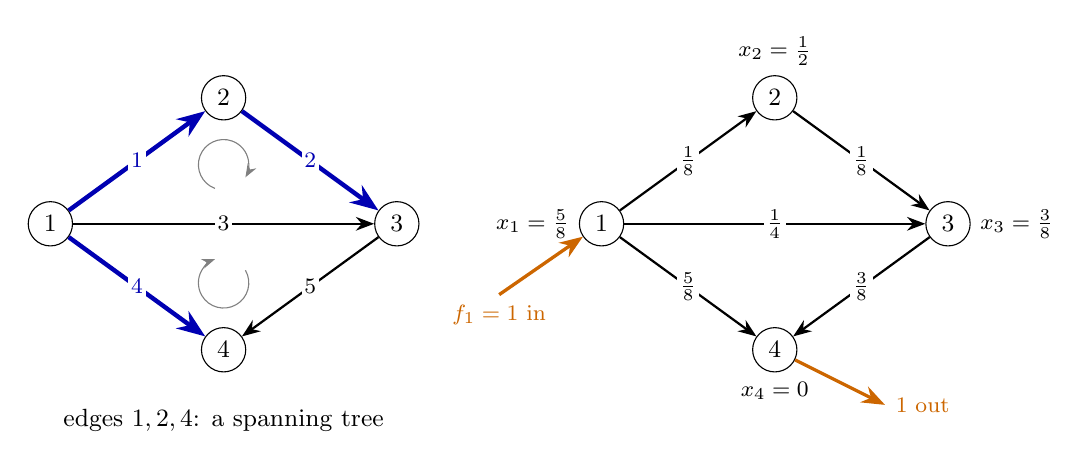
\begin{tikzpicture}[>=Stealth,font=\small,
    nd/.style={circle,draw,fill=white,inner sep=1.5pt,minimum size=16pt},
    el/.style={fill=white,inner sep=1pt,font=\footnotesize}]
  \begin{scope}
    \node[nd] (a) at (0,0) {1};
    \node[nd] (b) at (2.2,1.6) {2};
    \node[nd] (c) at (4.4,0) {3};
    \node[nd] (d) at (2.2,-1.6) {4};
    \draw[->,line width=1.6pt,blue!70!black] (a) -- node[el] {1} (b);
    \draw[->,line width=1.6pt,blue!70!black] (b) -- node[el] {2} (c);
    \draw[->,thick] (a) -- node[el] {3} (c);
    \draw[->,line width=1.6pt,blue!70!black] (a) -- node[el] {4} (d);
    \draw[->,thick] (c) -- node[el] {5} (d);
    \draw[->,gray] (2.2,0.75) ++(250:0.32) arc[start angle=250,end angle=-30,radius=0.32];
    \draw[->,gray] (2.2,-0.75) ++(30:0.32) arc[start angle=30,end angle=-250,radius=0.32];
    \node at (2.2,-2.5) {edges $1,2,4$: a spanning tree};
  \end{scope}
  \begin{scope}[xshift=7cm]
    \node[nd,label={[font=\footnotesize]left:$x_1=\tfrac58$}] (a) at (0,0) {1};
    \node[nd,label={[font=\footnotesize]above:$x_2=\tfrac12$}] (b) at (2.2,1.6) {2};
    \node[nd,label={[font=\footnotesize]right:$x_3=\tfrac38$}] (c) at (4.4,0) {3};
    \node[nd,label={[font=\footnotesize]below:$x_4=0$}] (d) at (2.2,-1.6) {4};
    \draw[->,thick] (a) -- node[el] {$\tfrac18$} (b);
    \draw[->,thick] (b) -- node[el] {$\tfrac18$} (c);
    \draw[->,thick] (a) -- node[el] {$\tfrac14$} (c);
    \draw[->,thick] (a) -- node[el] {$\tfrac58$} (d);
    \draw[->,thick] (c) -- node[el] {$\tfrac38$} (d);
    \draw[->,very thick,orange!80!black] (-1.3,-0.9) -- (a) node[pos=0,below,font=\footnotesize] {$f_1=1$ in};
    \draw[->,very thick,orange!80!black] (d) -- (3.6,-2.3) node[right,font=\footnotesize] {$1$ out};
    \node at (2.2,-2.5) {};
  \end{scope}
\end{tikzpicture}
\caption{Left: the directed graph of Example~\ref{ex:u13-graph}; the two circular arrows mark
the independent loops (edges $1,2,3$ and edges $3,5,4$), and the thick edges $1,2,4$ form a tree.
Right: with unit conductances, one unit of current entering node~1 and leaving node~4
(Example~\ref{ex:u13-network}): node potentials and edge currents, all flowing along the arrows.}
\label{fig:u13-graph}
\end{figure}

\subsection{Potentials and the nullspace}

Multiply $A$ by a vector $\vb{x}=(x_1,x_2,x_3,x_4)$ of \emph{potentials} at the nodes:
\[
A\vb{x}=\begin{bmatrix}x_2-x_1\\x_3-x_2\\x_3-x_1\\x_4-x_1\\x_4-x_3\end{bmatrix}.
\]
Each component is a \emph{potential difference} across an edge (head minus tail). Potential
differences are what make current flow.

\begin{proposition}[Nullspace of an incidence matrix]\label{prop:u13-null}
If the graph is connected (every two nodes are joined by a path), then $\Nul{A}$ is the line of
constant vectors $c(1,1,\dots,1)$, and $\rank A=n-1$.
\end{proposition}
\begin{proof}
A constant vector gives zero differences, so it lies in $\Nul{A}$. Conversely, $A\vb{x}=\vb{0}$
says $x_i=x_j$ whenever an edge joins $i$ and $j$; following a path from node~1 to any node $k$
gives $x_k=x_1$. So $\dim\Nul{A}=1$ and $r=n-1$.
\end{proof}

Physically, potentials are determined only up to an additive constant, like the constant of
integration in calculus or the choice of zero on a temperature scale. One fixes it by
\emph{grounding} a node, say $x_4=0$. That removes column~4, and the remaining three columns are
independent. In the example $r=3$, and any three of the four columns are independent.

Which vectors $\vb{e}$ of edge values are potential differences, i.e.\ lie in $\Col{A}$? Going around
a loop, the differences telescope: on the loop of edges $1,2,3$,
$(x_2-x_1)+(x_3-x_2)-(x_3-x_1)=0$. So every $\vb{e}=A\vb{x}$ satisfies $e_1+e_2-e_3=0$, and
likewise $e_3+e_5-e_4=0$ on the other loop. This is \emph{Kirchhoff's voltage law}, and by
Theorem~\ref{thm:u09-solvable} these loop conditions are also sufficient once we know that the loop
vectors span the left nullspace, which we prove next.

\subsection{Currents and Kirchhoff's current law}

Now let $\vb{y}=(y_1,\dots,y_5)$ be \emph{currents} on the edges, positive when flowing along the
arrow. Then
\[
A\T\vb{y}=\begin{bmatrix}-1&0&-1&-1&0\\1&-1&0&0&0\\0&1&1&0&-1\\0&0&0&1&1\end{bmatrix}
\begin{bmatrix}y_1\\y_2\\y_3\\y_4\\y_5\end{bmatrix}
=\begin{bmatrix}-y_1-y_3-y_4\\y_1-y_2\\y_2+y_3-y_5\\y_4+y_5\end{bmatrix}.
\]
Row $i$ of $A\T\vb{y}$ is (current into node $i$) minus (current out of node $i$). The equation
\[
A\T\vb{y}=\vb{0}\qquad\text{(Kirchhoff's current law)}
\]
says that at every node, in equals out: charge does not accumulate. It is a balance equation, a
conservation law, perhaps the most fundamental equation of applied mathematics. Its solutions form
the left nullspace, of dimension $m-r=5-3=2$.

\begin{definition}[Loop vector]\label{def:u13-loop}
For a loop in the graph traversed in a chosen direction, its \emph{loop vector} has entry $+1$ for
each edge traversed along its arrow, $-1$ for each edge traversed against its arrow, and $0$ for
edges not on the loop.
\end{definition}

\begin{theorem}[Loops span the left nullspace]\label{thm:u13-loops}
Every loop vector satisfies $A\T\vb{y}=\vb{0}$, and every solution of $A\T\vb{y}=\vb{0}$ is a
combination of loop vectors.
\end{theorem}
\begin{proof}
A loop vector sends one unit of current around the loop. At each node on the loop, one unit
arrives along one loop edge and one unit leaves along the next, so in minus out is $0$; nodes off
the loop see no current.

Conversely, let $\vb{y}\ne\vb{0}$ satisfy the current law. Pick an edge with $y_k\ne0$ and walk along
it in the direction the current flows. At the node reached, current arrives, so by the balance
some other edge carries current away; walk along it in its direction of flow. Continue. With
finitely many nodes, the walk eventually revisits a node, closing a loop on which every edge carries
nonzero current in the walking direction. Let $t>0$ be the smallest of these currents in absolute
value and subtract $t$ times this loop's vector from $\vb{y}$. The result still satisfies the
current law and has at least one more zero entry. Repeating, after finitely many steps nothing is
left, so $\vb{y}$ was a sum of multiples of loop vectors.
\end{proof}

\begin{example}[Two independent loops]\label{ex:u13-loops}
Send one unit around the upper triangle $1\to2\to3\to1$: edges $1$ and $2$ are traversed along
their arrows and edge~$3$ against it, giving $\vb{y}=(1,1,-1,0,0)$. Check the four node equations:
$-1+1-0=0$, $1-1=0$, $1-1-0=0$, $0+0=0$. The lower triangle $1\to3\to4\to1$ gives
$(0,0,1,-1,1)$. These two are independent (look at entries $1$ and $5$), and $\dim\Nul{A\T}=2$,
so they form a basis. The big outer loop $1\to2\to3\to4\to1$ gives $(1,1,0,-1,1)$, which is
their sum: on edge~3 the two loop currents cancel. It is a loop, but not an independent one.
\end{example}

\subsection{Trees, the row space and Euler's formula}

The row space $\Col{A\T}$ has dimension $r=3$. Which three rows (edges) are independent? Row
reduction of $A\T$ finds pivots in columns $1,2,4$, the columns of $A\T$ that belong to edges $1,2$
and~$4$. Column~3 of $A\T$ is column~1 plus column~2, which is the loop $1,2,3$ again. The pivot edges
$1,2,4$ connect all four nodes and contain no loop (thick edges in Figure~\ref{fig:u13-graph}).
A graph with no loops is a \emph{tree}. Independent rows correspond to edges without loops;
dependencies among rows are exactly loops.

\begin{theorem}[Euler's formula]\label{thm:u13-euler}
For a connected graph with $n$ nodes, $m$ edges and $\ell=\dim\Nul{A\T}$ independent loops,
\[
n-m+\ell=1.
\]
\end{theorem}
\begin{proof}
By Theorem~\ref{thm:u11-dims}, $\ell=\dim\Nul{A\T}=m-r$, and $r=n-1$ by
Proposition~\ref{prop:u13-null}. So $\ell=m-n+1$.
\end{proof}

Nodes are zero-dimensional, edges one-dimensional, and loops enclose two-dimensional regions; the
alternating count is always $1$. For the example, $4-5+2=1$. For a graph with $5$ nodes and $7$
edges drawn in the plane with $3$ independent loops, $5-7+3=1$. Linear algebra has proved a theorem
of topology.

\begin{trap}
Euler's formula counts \emph{independent} loops. The graph of Figure~\ref{fig:u13-graph} has three
visible loops (two triangles and the outer quadrilateral), and $4-5+3\neq1$; the outer loop is the
sum of the other two. Also, Proposition~\ref{prop:u13-null} needs a connected graph: if the graph
falls into separate pieces, $\Nul{A}$ is larger (Exercise~\ref{exr:u13-disconnected}).
\end{trap}

\subsection{\texorpdfstring{Ohm's law and \(A\T CA\vb{x}=\vb{f}\)}{Ohm's law and ATCAx = f}}

The three steps of an electrical network chain together:
\begin{center}
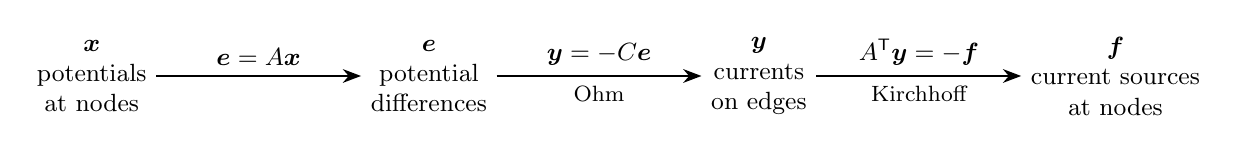
\begin{tikzpicture}[>=Stealth,font=\small,node distance=2.6cm]
  \node[align=center] (x) {$\vb{x}$\\potentials\\at nodes};
  \node[align=center,right=of x] (e) {$\vb{e}$\\potential\\differences};
  \node[align=center,right=of e] (y) {$\vb{y}$\\currents\\on edges};
  \node[align=center,right=of y] (f) {$\vb{f}$\\current sources\\at nodes};
  \draw[->,thick] (x) -- node[above] {$\vb{e}=A\vb{x}$} (e);
  \draw[->,thick] (e) -- node[above] {$\vb{y}=-C\vb{e}$} node[below,font=\footnotesize] {Ohm} (y);
  \draw[->,thick] (y) -- node[above] {$A\T\vb{y}=-\vb{f}$} node[below,font=\footnotesize] {Kirchhoff} (f);
\end{tikzpicture}
\end{center}
Ohm's law says that the current on an edge is its conductance (one over its resistance) times the
potential drop; $C$ is the diagonal matrix of conductances. Current flows from high to low
potential, hence the minus sign in $\vb{y}=-C\vb{e}$. If a current $f_i$ is fed into node $i$ from
outside, the balance at that node becomes (in) $-$ (out) $+f_i=0$, i.e.\ $A\T\vb{y}=-\vb{f}$.
Combining the three equations, the signs cancel:
\[
A\T CA\,\vb{x}=\vb{f}.
\]
(The lecture writes the chain as $\vb{e}=A\vb{x}$, $\vb{y}=C\vb{e}$, $A\T\vb{y}=\vb{f}$, absorbing
the signs into the conventions; the resulting equation is the same.) This is the basic equation of
equilibrium for networks, and the matrix $A\T CA$ is symmetric:
$(A\T CA)\T=A\T C\T A=A\T CA$.

\begin{proposition}[The matrix \texorpdfstring{\(A\T A\)}{ATA} of a graph]\label{prop:u13-laplacian}
For an incidence matrix $A$, the diagonal entry $(A\T A)_{ii}$ is the \emph{degree} of node $i$
(the number of edges touching it), the off-diagonal entry $(A\T A)_{ij}$ is $-1$ if an edge joins
$i$ and $j$ and $0$ otherwise, and $\tr(A\T A)=2m$.
\end{proposition}
\begin{proof}
$(A\T A)_{ij}$ is the dot product of columns $i$ and $j$ of $A$. Column $i$ has an entry $\pm1$ in
each row whose edge touches node $i$, so its squared length is the degree. Two different columns
share a nonzero row only for an edge joining $i$ and $j$, where the entries are $-1$ and $+1$. The
trace is the sum of the degrees, and each edge contributes to two degrees.
\end{proof}

\begin{example}[Solving a network]\label{ex:u13-network}
Take all conductances equal to $1$ ($C=I$) in the graph of Example~\ref{ex:u13-graph}, feed one unit
of current into node~1 and take it out at node~4: $\vb{f}=(1,0,0,-1)$. The degrees are $3,2,3,2$, so
\[
A\T A=\begin{bmatrix}3&-1&-1&-1\\-1&2&-1&0\\-1&-1&3&-1\\-1&0&-1&2\end{bmatrix}.
\]
It is singular (its rows add to zero, reflecting $\Nul{A}$), so ground node~4: set $x_4=0$ and
drop the fourth equation. The remaining equations $3x_1-x_2-x_3=1$, $-x_1+2x_2-x_3=0$,
$-x_1-x_2+3x_3=0$ give, by elimination, $\vb{x}=(\tfrac58,\tfrac12,\tfrac38,0)$. Check the first:
$\tfrac{15}{8}-\tfrac48-\tfrac38=1$. The potential differences and currents are
\[
\vb{e}=A\vb{x}=\bigl(-\tfrac18,-\tfrac18,-\tfrac14,-\tfrac58,-\tfrac38\bigr),\qquad
\vb{y}=-\vb{e}=\bigl(\tfrac18,\tfrac18,\tfrac14,\tfrac58,\tfrac38\bigr).
\]
All currents are positive, so all flow along the arrows (Figure~\ref{fig:u13-graph}, right). Node~1
sends out $\tfrac18+\tfrac14+\tfrac58=1$, node~2 passes $\tfrac18$ through, node~3 receives
$\tfrac18+\tfrac14$ and sends $\tfrac38$, and node~4 collects $\tfrac58+\tfrac38=1$. The direct edge
$1\to4$ carries the most current, because every other route to node~4 crosses two edges.
\end{example}

\subsection{Exercises}

\begin{exercise}\label{exr:u13-square}
A square graph has nodes $1,2,3,4$ and edges $1\to2$, $2\to3$, $4\to3$, $1\to4$ (in that order).
Write its $4\times4$ incidence matrix $A$. Which vectors are in $\Nul{A}$? Why is $(1,0,0,0)$ not in
the row space of $A$?
\end{exercise}
\begin{solution}
\[
A=\begin{bmatrix}-1&1&0&0\\0&-1&1&0\\0&0&1&-1\\-1&0&0&1\end{bmatrix},\qquad
A\vb{x}=\begin{bmatrix}x_2-x_1\\x_3-x_2\\x_3-x_4\\x_4-x_1\end{bmatrix}.
\]
$A\vb{x}=\vb{0}$ forces $x_1=x_2=x_3=x_4$, so $\Nul{A}$ is all $(a,a,a,a)$. Every row of $A$ has
entries adding to $0$ (one $-1$ and one $+1$), so every combination of rows has entries adding to
$0$; the entries of $(1,0,0,0)$ add to $1$, so it is not in the row space.
\end{solution}

\begin{exercise}\label{exr:u13-ATCA}
For the square graph of Exercise~\ref{exr:u13-square} let the conductances be
$C=\operatorname{diag}(1,2,2,1)$. Find $A\T CA$. For the current source $\vb{f}=(1,0,-1,0)$ (one
unit into node~1, out of node~3), solve $A\T CA\vb{x}=\vb{f}$ with node~3 grounded, and find the
currents $\vb{y}=-CA\vb{x}$.
\end{exercise}
\begin{solution}
Multiplying out (or using Proposition~\ref{prop:u13-laplacian} with each edge weighted by its
conductance),
\[
A\T CA=\begin{bmatrix}2&-1&0&-1\\-1&3&-2&0\\0&-2&4&-2\\-1&0&-2&3\end{bmatrix}.
\]
With $x_3=0$, the equations from nodes $1,2,4$ are $2x_1-x_2-x_4=1$, $-x_1+3x_2=0$,
$-x_1+3x_4=0$. So $x_2=x_4=x_1/3$ and $2x_1-\tfrac23x_1=1$, giving $x_1=\tfrac34$ and
$\vb{x}=(\tfrac34,\tfrac14,0,\tfrac14)$. Then $A\vb{x}=(-\tfrac12,-\tfrac14,-\tfrac14,-\tfrac12)$ and
$\vb{y}=-CA\vb{x}=(\tfrac12,\tfrac12,\tfrac12,\tfrac12)$: half the current takes the route
$1\to2\to3$ and half takes $1\to4\to3$, as symmetry demands (each route has conductances $1$ and $2$
in series). Check at node~1: $\tfrac12+\tfrac12=1$ leaves.
\end{solution}

\begin{exercise}\label{exr:u13-five}
A graph has $5$ nodes and $6$ edges: $1\to2$, $2\to3$, $1\to3$, $2\to4$, $4\to5$, $5\to3$. Without
row reduction, find $\Nul{A}$, a basis of $\Nul{A\T}$, and $\tr(A\T A)$.
\end{exercise}
\begin{solution}
The graph is connected, so $\Nul{A}$ is the line through $(1,1,1,1,1)$ and $r=4$; then
$\dim\Nul{A\T}=6-4=2$. Loop vectors: the triangle $1\to2\to3\to1$ gives $(1,1,-1,0,0,0)$, and the
square $2\to4\to5\to3\to2$ gives $(0,-1,0,1,1,1)$ (edge~2 is traversed against its arrow). They are
independent, so they form a basis; the outer loop $1\to2\to4\to5\to3\to1$ gives their sum
$(1,0,-1,1,1,1)$. The degrees are $2,3,3,2,2$, so $\tr(A\T A)=12=2m$.
\end{solution}

\begin{exercise}\label{exr:u13-disconnected}
A graph consists of two separate triangles: nodes $1,2,3$ with edges $1\to2$, $2\to3$, $1\to3$, and
nodes $4,5,6$ with edges $4\to5$, $5\to6$, $4\to6$. Find $\dim\Nul{A}$, the rank, and
$\dim\Nul{A\T}$. What becomes of Euler's formula?
\end{exercise}
\begin{solution}
$A\vb{x}=\vb{0}$ forces equal potentials within each triangle but not across, so $\Nul{A}$ has basis
$(1,1,1,0,0,0)$ and $(0,0,0,1,1,1)$: dimension $2$, rank $6-2=4$. Then
$\dim\Nul{A\T}=m-r=6-4=2$, one loop per triangle. Now $n-m+\ell=6-6+2=2$: in general the alternating
count equals the number of connected pieces, and Euler's formula is the case of one piece.
\end{solution}

% unit: u14
% sources: sources/005-exam-1-review.txt, sources/022-exam-1-review.txt, sources/103-mit18-06scf11-ses1-14sum-pdf-download-file.txt, sources/006-exam-1-problem-solving.txt
\section{Exam 1 review}\label{sec:u14}

The first exam covers Part I, Sections~\ref{sec:u01}--\ref{sec:u13}, with the emphasis on
rectangular matrices: nullspaces, ranks, complete solutions and the four subspaces. This section
collects the essential facts in one place and then works through the review problems of the course,
which test understanding by approaching familiar ideas from unfamiliar directions, for instance by
giving the answer and asking for the matrix.

\subsection{The essentials of Part I}

\begin{itemize}
\item \textbf{Elimination} (Sections~\ref{sec:u03}--\ref{sec:u05}). Row operations are
multiplications by elementary matrices: $E_{32}E_{31}E_{21}A=U$, so $A=LU$ with the multipliers in
$L$ (with row exchanges, $PA=LU$). Gauss--Jordan reduces $\begin{bmatrix}A&I\end{bmatrix}$ to
$\begin{bmatrix}I&A^{-1}\end{bmatrix}$ when $A$ is invertible.
\item \textbf{Subspaces} (Sections~\ref{sec:u06}--\ref{sec:u07}). A subspace contains $\vb{0}$ and
is closed under addition and scalar multiplication. Intersections of subspaces are subspaces;
unions usually are not.
\item \textbf{Rank and special solutions} (Section~\ref{sec:u08}). $r=$ number of pivots;
$R=\operatorname{rref}(A)$ has the block form $\begin{bmatrix}I&F\\0&0\end{bmatrix}$ (pivot columns
first), and the special solutions are the columns of $N=\begin{bmatrix}-F\\I\end{bmatrix}$.
\item \textbf{Complete solution} (Section~\ref{sec:u09}). $A\vb{x}=\vb{b}$ is solvable iff
$\vb{b}\in\Col{A}$; then $\vb{x}=\vb{x}_p+\vb{x}_n$. Full column rank $r=n$: at most one solution;
full row rank $r=m$: at least one (Table~\ref{tab:u09-cases}).
\item \textbf{Basis and dimension} (Section~\ref{sec:u10}). Independent and spanning; every basis of
a space has the same size. Pivot columns of $A$ are a basis of $\Col{A}$.
\item \textbf{Four subspaces} (Section~\ref{sec:u11}). Dimensions $r$, $n-r$, $r$, $m-r$ for
$\Col{A}$, $\Nul{A}$, $\Col{A\T}$, $\Nul{A\T}$. Row operations preserve the row space and the
nullspace.
\item \textbf{Beyond $\R^n$} (Sections~\ref{sec:u12}--\ref{sec:u13}). Spaces of matrices and
functions; rank one means $\vb{u}\vb{v}\T$; for a connected graph, $\Nul{A}$ is the constants,
$\Nul{A\T}$ is spanned by loops, and $n-m+\ell=1$.
\end{itemize}

Figure~\ref{fig:u14-flow} is the algorithm for $A\vb{x}=\vb{b}$ that runs through all of it.

\begin{figure}[ht]\centering
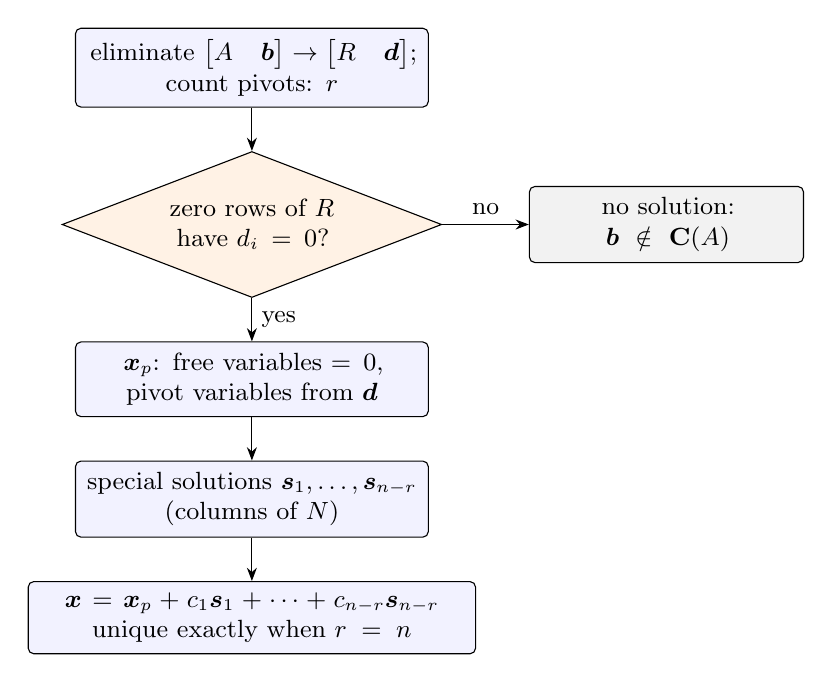
\begin{tikzpicture}[>=Stealth,font=\small,node distance=0.55cm,
    box/.style={draw,rounded corners=2pt,fill=blue!5,align=center,inner sep=4pt,text width=4.2cm},
    dec/.style={draw,diamond,aspect=2.6,fill=orange!10,align=center,inner sep=1pt,text width=2.9cm}]
  \node[box] (elim) {eliminate $\begin{bmatrix}A&\vb{b}\end{bmatrix}\to\begin{bmatrix}R&\vb{d}\end{bmatrix}$;\\ count pivots: $r$};
  \node[dec,below=of elim] (test) {zero rows of $R$\\have $d_i=0$?};
  \node[box,right=1.1cm of test,text width=3.2cm,fill=gray!10] (none) {no solution:\\$\vb{b}\notin\Col{A}$};
  \node[box,below=of test] (xp) {$\vb{x}_p$: free variables $=0$,\\pivot variables from $\vb{d}$};
  \node[box,below=of xp] (xn) {special solutions $\vb{s}_1,\dots,\vb{s}_{n-r}$\\(columns of $N$)};
  \node[box,below=of xn,text width=5.4cm] (all) {$\vb{x}=\vb{x}_p+c_1\vb{s}_1+\dots+c_{n-r}\vb{s}_{n-r}$\\unique exactly when $r=n$};
  \draw[->] (elim) -- (test);
  \draw[->] (test) -- node[above] {no} (none);
  \draw[->] (test) -- node[right] {yes} (xp);
  \draw[->] (xp) -- (xn);
  \draw[->] (xn) -- (all);
\end{tikzpicture}
\caption{Solving $A\vb{x}=\vb{b}$ for any $m\times n$ matrix. When $r=m$ there are no zero rows and
the test always passes; when $r=n$ there are no special solutions.}
\label{fig:u14-flow}
\end{figure}

\subsection{Solved review problems}

\begin{example}[The dimension of a span]\label{ex:u14-span}
\emph{Nonzero vectors $\vb{u},\vb{v},\vb{w}\in\R^7$ span a subspace. What are its possible
dimensions?}
The answer is $1$, $2$ or $3$. A basis can be chosen from among the three spanning vectors, so the
dimension is at most $3$; it is at least $1$ because the vectors are nonzero. All three values
occur: $\vb{u}=\vb{v}=\vb{w}$ gives $1$, and three independent vectors give $3$.
\end{example}

\begin{example}[Stacked echelon forms]\label{ex:u14-blocks}
\emph{A $5\times3$ matrix $R$ in reduced echelon form has $r=3$ pivots. (a) Find $\Nul{R}$. (b) Find
the reduced echelon form and the rank of the $10\times3$ matrix $B=\begin{bmatrix}R\\2R\end{bmatrix}$.
(c) Do the same for the $10\times6$ matrix $C=\begin{bmatrix}R&R\\R&0\end{bmatrix}$. (d) Find
$\dim\Nul{C\T}$.}

(a) Three pivots in three columns: no free variables, so $\Nul{R}=\{\vb{0}\}$. In fact
$R=\begin{bmatrix}I_3\\0\end{bmatrix}$ is forced: three pivots equal to $1$, zeros elsewhere in
their columns, two zero rows.

(b) Subtract $2\times$(rows $1$--$5$) from rows $6$--$10$: $B\to\begin{bmatrix}R\\0\end{bmatrix}$,
which is already in reduced form. The rank is $3$, not $6$: the bottom rows of $B$ are multiples of
the top rows.

(c) Work with block rows. Subtract the top block row from the bottom one, then add the new bottom
block row to the top one, then multiply the bottom by $-1$:
\[
\begin{bmatrix}R&R\\R&0\end{bmatrix}\to\begin{bmatrix}R&R\\0&-R\end{bmatrix}\to
\begin{bmatrix}R&0\\0&-R\end{bmatrix}\to\begin{bmatrix}R&0\\0&R\end{bmatrix}.
\]
Moving the zero rows (rows $4,5$ and $9,10$) to the bottom gives
$\begin{bmatrix}I_6\\0\end{bmatrix}$. The rank is $6$.

(d) $C$ is $10\times6$ of rank $6$, so $\dim\Nul{C\T}=m-r=10-6=4$ (and $\dim\Nul{C}=6-6=0$).
\end{example}

\begin{example}[From the complete solution back to the matrix]\label{ex:u14-recover}
\emph{The complete solution of $A\vb{x}=(2,4,2)$ is}
\[
\vb{x}=\begin{bmatrix}2\\0\\0\end{bmatrix}+c\begin{bmatrix}1\\1\\0\end{bmatrix}+d\begin{bmatrix}0\\0\\1\end{bmatrix}.
\]
\emph{Find the shape of $A$, its rank, $A$ itself, and the $\vb{b}$ for which $A\vb{x}=\vb{b}$ is
solvable.}

$\vb{x}$ and $\vb{b}$ both have three components, so $A$ is $3\times3$. The two vectors multiplying
$c$ and $d$ are independent and lie in $\Nul{A}$; nothing else does (otherwise there would be more
free constants), so $\dim\Nul{A}=2$ and $r=3-2=1$. To recover $A$: $A(2,0,0)=2\,\vb{a}_1=(2,4,2)$
gives $\vb{a}_1=(1,2,1)$; $A(0,0,1)=\vb{a}_3=\vb{0}$; and $A(1,1,0)=\vb{a}_1+\vb{a}_2=\vb{0}$ gives
$\vb{a}_2=-\vb{a}_1$. Hence
\[
A=\begin{bmatrix}1&-1&0\\2&-2&0\\1&-1&0\end{bmatrix},\qquad
A\begin{bmatrix}2\\0\\0\end{bmatrix}=\begin{bmatrix}2\\4\\2\end{bmatrix}.
\]
$A\vb{x}=\vb{b}$ is solvable exactly when $\vb{b}\in\Col{A}$, i.e.\ when $\vb{b}$ is a multiple of
$(1,2,1)$. This is the case $r<m$, $r<n$: zero or infinitely many solutions.
\end{example}

\begin{example}[A factored matrix]\label{ex:u14-CD}
\emph{Let}
\[
B=CD=\begin{bmatrix}1&1&0\\0&1&0\\1&0&1\end{bmatrix}\begin{bmatrix}1&0&-1&2\\0&1&1&-1\\0&0&0&0\end{bmatrix}.
\]
\emph{Without multiplying, find a basis of $\Nul{B}$ and the complete solution of
$B\vb{x}=(1,0,1)$.}

$B$ is $3\times4$, so $\Nul{B}\subseteq\R^4$. The first factor $C$ is invertible: in a combination of
its columns giving $\vb{0}$, the second row forces the weight of column~2 to be $0$, and columns~1
and~3 are clearly independent. By Proposition~\ref{prop:u08-same-null}, $\Nul{CD}=\Nul{D}$, and $D$ is
already in reduced form with pivot columns $1,2$ and $F=\begin{bmatrix}-1&2\\1&-1\end{bmatrix}$.
The special solutions (columns of $\begin{bmatrix}-F\\I\end{bmatrix}$) are
\[
\vb{s}_1=(1,-1,1,0),\qquad\vb{s}_2=(-2,1,0,1),
\]
a basis of $\Nul{B}$ (and $\rank B=2$). For a particular solution, note that the first column of $B$
is $C$ times the first column of $D$, which is the first column of $C$, namely $(1,0,1)$, exactly the
right-hand side. So $\vb{x}_p=(1,0,0,0)$ and
\[
\vb{x}=\begin{bmatrix}1\\0\\0\\0\end{bmatrix}+c\begin{bmatrix}1\\-1\\1\\0\end{bmatrix}
+d\begin{bmatrix}-2\\1\\0\\1\end{bmatrix}.
\]
Any other solution would serve equally well as $\vb{x}_p$; this one is simply the most convenient.
\end{example}

\begin{example}[A square system with a parameter]\label{ex:u14-k}
\emph{Let $A=\begin{bmatrix}1&1&1\\1&2&3\\3&4&k\end{bmatrix}$ and $\vb{b}=(2,3,7)$. (a) For which $k$
does $A\vb{x}=\vb{b}$ have exactly one solution? (b) Infinitely many? (c) Find $A=LU$. (d) Find the
complete solution for every $k$.}

Eliminate on the augmented matrix and record the steps, since part (c) needs them. $E_{21}$ subtracts
row~1 from row~2, $E_{31}$ subtracts $3\times$row~1 from row~3, and $E_{32}$ subtracts row~2 from
row~3:
\[
\left[\begin{array}{ccc|c}1&1&1&2\\1&2&3&3\\3&4&k&7\end{array}\right]\to
\left[\begin{array}{ccc|c}1&1&1&2\\0&1&2&1\\0&1&k-3&1\end{array}\right]\to
\left[\begin{array}{ccc|c}1&1&1&2\\0&1&2&1\\0&0&k-5&0\end{array}\right].
\]
(a) The third pivot is $k-5$. For $k\ne5$, $A$ is invertible and the solution is unique.
(b) For $k=5$ the third row becomes $0=0$, consistent, and $x_3$ is free: infinitely many solutions.
(Had the last entry been nonzero, $k=5$ would give no solution at all.)
(c) $U$ is the final left block, and $L=E_{21}^{-1}E_{31}^{-1}E_{32}^{-1}$ holds the multipliers
$1,3,1$ in their positions:
\[
A=\begin{bmatrix}1&0&0\\1&1&0\\3&1&1\end{bmatrix}\begin{bmatrix}1&1&1\\0&1&2\\0&0&k-5\end{bmatrix}.
\]
(d) For $k\ne5$: $x_3=0$, then $x_2=1$, then $x_1=2-1-0=1$, so $\vb{x}=(1,1,0)$. For $k=5$: set
$x_3=c$; then $x_2=1-2c$ and $x_1=2-x_2-x_3=1+c$, so
\[
\vb{x}=\begin{bmatrix}1\\1\\0\end{bmatrix}+c\begin{bmatrix}1\\-2\\1\end{bmatrix}.
\]
Check: with $k=5$, $A(1,-2,1)=(1-2+1,\,1-4+3,\,3-8+5)=\vb{0}$.
\end{example}

\subsection{Quick checks}

The following short questions test whether the definitions are understood. Each answer is followed
by its reason.
\begin{enumerate}[1.]
\item \emph{$A$ is square and $\Nul{A}=\{\vb{0}\}$. What is $\Nul{A\T}$?} Also $\{\vb{0}\}$: $r=n=m$, so
$\dim\Nul{A\T}=m-r=0$.
\item \emph{Do the invertible $5\times5$ matrices form a subspace of the $25$-dimensional space of
$5\times5$ matrices?} No: the zero matrix is not invertible, and $I+(-I)=0$. (The singular matrices
fail too: $\operatorname{diag}(1,0)+\operatorname{diag}(0,1)=I$ in the $2\times2$ case.)
\item \emph{If $B^2=0$, must $B=0$?} No: $B=\begin{bmatrix}0&1\\0&0\end{bmatrix}$ has $B^2=0$.
\item \emph{An $n\times n$ system with independent columns is solvable for every $\vb{b}$.} True:
$r=n=m$, so $A$ is invertible and $\vb{x}=A^{-1}\vb{b}$.
\item \emph{If $m=n$, the row space equals the column space.} False: for
$B=\begin{bmatrix}0&1\\0&0\end{bmatrix}$ the row space is the line through $(0,1)$ and the column
space is the line through $(1,0)$. Only the dimensions agree. (For a symmetric matrix they are equal.)
\item \emph{$A$ and $-A$ have the same four subspaces.} True: each subspace contains $-\vb{v}$
whenever it contains $\vb{v}$.
\item \emph{If $A$ and $B$ have the same four subspaces, then $A$ is a multiple of $B$.} False: every
invertible $3\times3$ matrix has $\Col{A}=\Col{A\T}=\R^3$ and both nullspaces $\{\vb{0}\}$, yet
$I$ and $\operatorname{diag}(1,2,3)$ are not multiples of each other. What \emph{is} forced is equal
rank.
\item \emph{If two rows of $A$ are exchanged, which subspaces stay the same?} The row space and the
nullspace. The column space can change: exchanging the rows of $\begin{bmatrix}1&0\\0&0\end{bmatrix}$
moves $\Col{A}$ from the line through $(1,0)$ to the line through $(0,1)$.
\item \emph{Why can $\vb{v}=(1,2,3)$ not be both a row of $A$ and in $\Nul{A}$?} The entry of
$A\vb{v}$ in that row would be $\vb{v}\cdot\vb{v}=1+4+9=14\ne0$. In fact the row space and the
nullspace meet only in $\vb{0}$, and they are perpendicular, the first topic of Part II
(Section~\ref{sec:u16}).
\end{enumerate}

\begin{trap}
Stacking copies of rows does not add rank. In Example~\ref{ex:u14-blocks} it is tempting to say
$\rank\begin{bmatrix}R\\2R\end{bmatrix}=6$ because the matrix ``contains $R$ twice''; but rank
counts independent rows, and the rows of $2R$ are multiples of those of $R$. In
$\begin{bmatrix}R&R\\R&0\end{bmatrix}$, by contrast, the second block column breaks the dependence,
and the rank does double.
\end{trap}

\subsection{Exercises}

\begin{exercise}\label{exr:u14-dims}
$A$ is $3\times5$ of rank $3$. Give the dimensions of its four subspaces. Is $A\vb{x}=\vb{b}$
solvable for every $\vb{b}$? Can a solution be unique?
\end{exercise}
\begin{solution}
$\dim\Col{A}=3$, $\dim\Nul{A}=5-3=2$, $\dim\Col{A\T}=3$, $\dim\Nul{A\T}=3-3=0$. Since $r=m=3$,
$\Col{A}=\R^3$ and every $\vb{b}$ is reachable. Since $r<n$, there are two free variables, so every
solvable system has infinitely many solutions, never exactly one.
\end{solution}

\begin{exercise}\label{exr:u14-k}
For which numbers $k$ are $(1,1,0)$, $(0,1,1)$, $(1,0,k)$ linearly independent? For the exceptional
value, find the dependency.
\end{exercise}
\begin{solution}
Put them in the columns of $A=\begin{bmatrix}1&0&1\\1&1&0\\0&1&k\end{bmatrix}$ and eliminate:
row~2 $-$ row~1 gives $(0,1,-1)$, then row~3 $-$ row~2 gives $(0,0,k+1)$. Three pivots unless
$k=-1$, so the vectors are independent exactly when $k\ne-1$. For $k=-1$ the free variable
$x_3=1$ gives $x_2=1$ and $x_1=-1$: $-(1,1,0)+(0,1,1)+(1,0,-1)=\vb{0}$.
\end{solution}

\begin{exercise}\label{exr:u14-invertible}
$M$ is an invertible matrix. Which of the four subspaces of $A$ are unchanged in $MA$ (when $M$ is
$m\times m$)? Which are unchanged in $AM$ (when $M$ is $n\times n$)?
\end{exercise}
\begin{solution}
$MA$: the nullspace is unchanged ($MA\vb{x}=\vb{0}\iff A\vb{x}=\vb{0}$) and so is the row space
(the rows of $MA$ are combinations of the rows of $A$, and conversely via $M^{-1}$); this is
Theorem~\ref{thm:u11-row}. The column space and left nullspace may change, as row exchanges show.
$AM$: transposing, $(AM)\T=M\T A\T$ with $M\T$ invertible, so by the first part $A\T$ and $M\T A\T$
have the same nullspace and row space; that is, $AM$ has the same left nullspace and column space as
$A$. Its nullspace and row space may change. In every case the rank is unchanged.
\end{solution}

% unit: u15
% sources: sources/018-exam-1.txt, sources/113-mit18-06scf11-ex1-pdf-download-file.txt, sources/114-mit18-06scf11-ex1s-pdf-download-file.txt
\section{Exam 1}\label{sec:u15}

The first unit exam checks whether the machinery of Part~I has become reflex: elimination
written with elementary matrices $E_{ij}$, the factorization $A=LU$, the inverse, bases for
the column space and the nullspace, the complete solution of $A\vb{x}=\vb{b}$, and what the
reduced echelon form $R$ says about the columns of $A$. This section collects the four exam
problems as practice problems with complete solutions, preceded by the handful of facts they
draw on and followed by variations to practise on. Try each problem before reading its solution.

\subsection{The facts the exam draws on}

Every problem on the exam is an application of a few statements from
Sections~\ref{sec:u05}--\ref{sec:u11}. For an $m\times n$ matrix $A$ of rank $r$:
\begin{itemize}
  \item $A\vb{x}=\vb{b}$ is solvable exactly when $\vb{b}\in\Col{A}$; it is solvable for
    \emph{every} $\vb{b}\in\R^m$ exactly when $r=m$.
  \item A solution, when one exists, is unique exactly when $\Nul{A}=\{\vb{0}\}$, that is,
    when $r=n$. Otherwise the complete solution is $\vb{x}_p+\vb{x}_n$ with $\vb{x}_n$ ranging
    over the $(n-r)$-dimensional nullspace.
  \item The pivot columns of $A$ (not of $R$) are a basis for $\Col{A}$; the $n-r$ special
    solutions are a basis for $\Nul{A}$.
  \item Row operations do not change the nullspace, so $A$ and $R=\operatorname{rref}(A)$
    satisfy exactly the same column relations.
  \item The inverse of an elimination matrix $E_{ij}$ (subtract $\ell$ times row $j$ from row
    $i$) adds $\ell$ times row $j$ back, and the inverse of a product reverses the order.
\end{itemize}
The first two items combine into the four cases of Table~\ref{tab:u15-cases}, which is the
whole content of Problem~1 below.

\begin{table}[ht]
  \centering
  \begin{tabular}{@{}llll@{}}
    \toprule
    Rank & Shape of $R$ & Solutions of $A\vb{x}=\vb{b}$ & Example \\
    \midrule
    $r=m=n$ & $I$ & exactly one, for every $\vb{b}$ & square invertible \\
    $r=n<m$ & $\begin{bmatrix} I\\ 0\end{bmatrix}$ & zero or one & tall, independent columns \\
    $r=m<n$ & $\begin{bmatrix} I & F\end{bmatrix}$ & infinitely many, for every $\vb{b}$ & wide, independent rows \\
    $r<m,\ r<n$ & $\begin{bmatrix} I & F\\ 0 & 0\end{bmatrix}$ & zero or infinitely many & neither \\
    \bottomrule
  \end{tabular}
  \caption{Rank decides how many solutions $A\vb{x}=\vb{b}$ can have ($F$ is the free part of $R$; columns may need reordering).}
  \label{tab:u15-cases}
\end{table}

\begin{example}[Reading the case from two right-hand sides]\label{ex:u15-case}
Take
\[
  A=\begin{bmatrix}1&2\\2&4\\3&6\end{bmatrix}.
\]
Column~2 is twice column~1, so $r=1$, which is smaller than both $m=3$ and $n=2$: the last
row of the table. Check both possibilities. For $\vb{b}=(1,2,3)$, which is column~1, the
system is solvable with $\vb{x}_p=(1,0)$, and adding any multiple of the special solution
$(-2,1)$ gives infinitely many solutions $\vb{x}=(1-2t,\,t)$. For $\vb{b}=(1,0,0)$,
elimination on the augmented matrix gives
\[
  \left[\begin{array}{cc|c}1&2&1\\2&4&0\\3&6&0\end{array}\right]
  \longrightarrow
  \left[\begin{array}{cc|c}1&2&1\\0&0&-2\\0&0&-3\end{array}\right],
\]
and the equations $0=-2$ and $0=-3$ are impossible, so there is no solution. A single
right-hand side with a unique solution would have forced $r=n$; a single unsolvable one
forces $r<m$.
\end{example}

\subsection{Problem 1: rank from solvability}

\begin{exercise}[Exam problem 1]\label{ex:u15-p1}
An $m\times n$ matrix $A$ has the property that
\[
  A\vb{x}=\begin{bmatrix}1\\1\\1\end{bmatrix}\ \text{has no solution}
  \qquad\text{and}\qquad
  A\vb{x}=\begin{bmatrix}0\\1\\0\end{bmatrix}\ \text{has exactly one solution.}
\]
\begin{enumerate}[(a)]
  \item Give all the information you can about $m$, $n$ and the rank $r$.
  \item Find all solutions of $A\vb{x}=\vb{0}$ and explain.
  \item Write down an example of such a matrix $A$.
\end{enumerate}
\end{exercise}

\begin{solution}
(a) The right-hand sides live in $\R^m$, so $m=3$. Exactly one solution for
$\vb{b}=(0,1,0)$ means there are no free variables: $\Nul{A}=\{\vb{0}\}$ and $r=n$. No
solution for $\vb{b}=(1,1,1)$ means $\Col{A}\neq\R^3$, so $r<m=3$. Together,
$r=n\le 2$: either $n=r=1$ or $n=r=2$ (and $m=3$ in both cases).

(b) Since $r=n$, the columns are independent and $A\vb{x}=\vb{0}$ has only the solution
$\vb{x}=\vb{0}$. (The zero vector is always a solution; independence of the columns says no
other combination of them vanishes.)

(c) Two examples, one for each possible $n$:
\[
  n=1:\ A=\begin{bmatrix}0\\1\\0\end{bmatrix},\qquad
  n=2:\ A=\begin{bmatrix}1&0\\0&1\\0&0\end{bmatrix}.
\]
For $n=1$, $A\vb{x}=(0,1,0)$ is solved only by the scalar $x=1$, and $(1,1,1)$ is not a
multiple of $(0,1,0)$. For $n=2$ the column space is the plane $x_3=0$
(Figure~\ref{fig:u15-p1}), which contains $(0,1,0)=A(0,1)$ but not $(1,1,1)$; the two
columns are independent, so the solution $(0,1)$ is unique.
\end{solution}

\begin{figure}[ht]
  \centering
  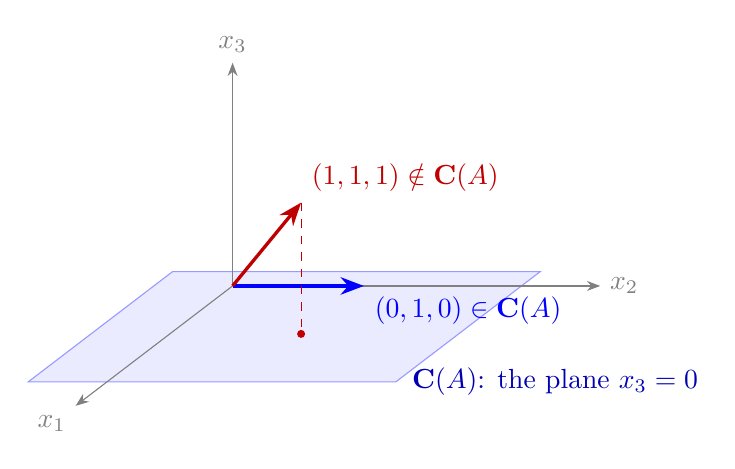
\begin{tikzpicture}[x={(-0.55cm,-0.42cm)},y={(1.15cm,0cm)},z={(0cm,1.15cm)},>=Stealth,scale=1.45]
    \fill[blue!8] (-0.3,-0.6,0) -- (2,-0.6,0) -- (2,2.2,0) -- (-0.3,2.2,0) -- cycle;
    \draw[blue!40] (-0.3,-0.6,0) -- (2,-0.6,0) -- (2,2.2,0) -- (-0.3,2.2,0) -- cycle;
    \draw[->,gray] (0,0,0) -- (2.5,0,0) node[below left] {$x_1$};
    \draw[->,gray] (0,0,0) -- (0,2.8,0) node[right] {$x_2$};
    \draw[->,gray] (0,0,0) -- (0,0,1.7) node[above] {$x_3$};
    \draw[->,very thick,blue] (0,0,0) -- (0,1,0) node[below right] {$(0,1,0)\in\Col{A}$};
    \draw[->,very thick,red!75!black] (0,0,0) -- (1,1,1) node[above right] {$(1,1,1)\notin\Col{A}$};
    \draw[dashed,red!75!black] (1,1,1) -- (1,1,0);
    \fill[red!75!black] (1,1,0) circle (1pt);
    \node[blue!70!black,anchor=west] at (2,2.25,0) {$\Col{A}$: the plane $x_3=0$};
  \end{tikzpicture}
  \caption{Problem 1(c) with $n=2$: the column space of $A$ is a plane through the origin in $\R^3$.
  Right-hand sides in the plane are reachable (uniquely, since the columns are independent);
  $(1,1,1)$ sits above the plane and is not.}
  \label{fig:u15-p1}
\end{figure}

\begin{trap}
Each hypothesis controls one inequality: uniqueness for one $\vb{b}$ gives $r=n$ (no free
variables), unsolvability for one $\vb{b}$ gives $r<m$. A frequent slip is to read ``exactly
one solution'' as ``$A$ is square and invertible''; that would make every $\vb{b}$ solvable,
contradicting the first hypothesis.
\end{trap}

\subsection{Problem 2: from elimination matrices to \texorpdfstring{$A^{-1}$}{A inverse}, \texorpdfstring{$A$}{A} and \texorpdfstring{$L$}{L}}

\begin{exercise}[Exam problem 2]\label{ex:u15-p2}
A $3\times 3$ matrix $A$ reduces to $I$ by three row operations, in this order:
$E_{21}$ subtracts $4$ times row~1 from row~2; $E_{31}$ subtracts $3$ times row~1 from
row~3; $E_{23}$ subtracts row~3 from row~2.
\begin{enumerate}[(a)]
  \item Write $A^{-1}$ in terms of the $E$'s, then compute it.
  \item What is the original matrix $A$?
  \item What is the lower triangular factor $L$ in $A=LU$?
\end{enumerate}
\end{exercise}

\begin{solution}
(a) The operations give $E_{23}E_{31}E_{21}A=I$, so $A^{-1}=E_{23}E_{31}E_{21}$, with
\[
  E_{21}=\begin{bmatrix}1&0&0\\-4&1&0\\0&0&1\end{bmatrix},\quad
  E_{31}=\begin{bmatrix}1&0&0\\0&1&0\\-3&0&1\end{bmatrix},\quad
  E_{23}=\begin{bmatrix}1&0&0\\0&1&-1\\0&0&1\end{bmatrix}.
\]
Apply them to $I$ in order. $E_{31}E_{21}$ places $-4$ and $-3$ in column~1; then $E_{23}$
subtracts row~3 from row~2:
\[
  E_{31}E_{21}=\begin{bmatrix}1&0&0\\-4&1&0\\-3&0&1\end{bmatrix},\qquad
  A^{-1}=E_{23}(E_{31}E_{21})=\begin{bmatrix}1&0&0\\-1&1&-1\\-3&0&1\end{bmatrix}.
\]
(b) Invert the product in reverse order, $A=E_{21}^{-1}E_{31}^{-1}E_{23}^{-1}$, where each
inverse just flips the sign of its off-diagonal entry:
\[
  A=\begin{bmatrix}1&0&0\\4&1&0\\0&0&1\end{bmatrix}
    \begin{bmatrix}1&0&0\\0&1&0\\3&0&1\end{bmatrix}
    \begin{bmatrix}1&0&0\\0&1&1\\0&0&1\end{bmatrix}
   =\begin{bmatrix}1&0&0\\4&1&0\\3&0&1\end{bmatrix}
    \begin{bmatrix}1&0&0\\0&1&1\\0&0&1\end{bmatrix}
   =\begin{bmatrix}1&0&0\\4&1&1\\3&0&1\end{bmatrix}.
\]
Check: multiplying this $A$ by the $A^{-1}$ of part (a) gives $I$.

(c) Forward elimination on $A$ uses only $E_{21}$ and $E_{31}$: subtracting $4$ (row~1) from
row~2 and $3$ (row~1) from row~3 leaves a matrix that is already upper triangular. The step $E_{23}$ is an \emph{upward} step (it clears the entry above the
last pivot), so it is not part of $A=LU$. The multipliers $4$ and $3$ go straight into $L$:
\[
  L=E_{21}^{-1}E_{31}^{-1}=\begin{bmatrix}1&0&0\\4&1&0\\3&0&1\end{bmatrix},\qquad
  U=E_{23}^{-1}=\begin{bmatrix}1&0&0\\0&1&1\\0&0&1\end{bmatrix},
\]
and indeed the factorization in (b) already reads $A=LU$.
\end{solution}

\begin{trap}
$A^{-1}$ is the product of the $E$'s in the order they were \emph{applied}
($E_{23}E_{31}E_{21}$, last step on the left); $A$ is the product of the inverses in the
\emph{opposite} order. Writing $A^{-1}=E_{21}E_{31}E_{23}$ gives a different matrix here,
because $E_{23}$ does not commute with $E_{31}$.
\end{trap}

\subsection{Problem 3: bases and the complete solution for a matrix with a parameter}

\begin{exercise}[Exam problem 3]\label{ex:u15-p3}
This $3\times 4$ matrix depends on $c$:
\[
  A=\begin{bmatrix}1&1&2&4\\3&c&2&8\\0&0&2&2\end{bmatrix}.
\]
\begin{enumerate}[(a)]
  \item For each $c$ find a basis for the column space of $A$.
  \item For each $c$ find a basis for the nullspace of $A$.
  \item For each $c$ find the complete solution of $A\vb{x}=(1,c,0)$.
\end{enumerate}
\end{exercise}

\begin{solution}
Subtract $3$ (row~1) from row~2:
\[
  \begin{bmatrix}1&1&2&4\\0&c-3&-4&-4\\0&0&2&2\end{bmatrix}.
\]
Everything depends on whether the entry $c-3$ is a pivot.

\emph{Case $c\neq 3$.} The pivots are in columns 1, 2, 3, so $r=3$. Dividing and clearing
upward gives
\[
  R=\begin{bmatrix}1&0&0&2\\0&1&0&0\\0&0&1&1\end{bmatrix}.
\]
(a) The pivot columns of $A$, namely $(1,3,0)$, $(1,c,0)$, $(2,2,2)$, are a basis for
$\Col{A}$. Since $r=m=3$ this column space is all of $\R^3$, so the standard basis would do
equally well.
(b) One free variable, $x_4$. Setting $x_4=1$ in $R\vb{x}=\vb{0}$ gives $x_1=-2$, $x_2=0$,
$x_3=-1$; the basis is $\vb{s}=(-2,0,-1,1)$.

\emph{Case $c=3$.} Row~2 becomes $(0,0,-4,-4)$; adding half of it to row~3 kills row~3, so
$r=2$ with pivots in columns 1 and 3:
\[
  R=\begin{bmatrix}1&1&0&2\\0&0&1&1\\0&0&0&0\end{bmatrix}.
\]
(a) Basis for $\Col{A}$: columns 1 and 3 of $A$, $(1,3,0)$ and $(2,2,2)$.
(b) Free variables $x_2$ and $x_4$. The special solutions are
$\vb{s}_1=(-1,1,0,0)$ (from $x_2=1,x_4=0$) and $\vb{s}_2=(-2,0,-1,1)$ (from $x_2=0,x_4=1$).

(c) The right-hand side $(1,c,0)$ is exactly column~2 of $A$, so $\vb{x}_p=(0,1,0,0)$ is a
particular solution for every $c$. Adding the nullspace:
\[
  c\neq 3:\ \ \vb{x}=\begin{bmatrix}0\\1\\0\\0\end{bmatrix}+x_4\begin{bmatrix}-2\\0\\-1\\1\end{bmatrix};
  \qquad
  c=3:\ \ \vb{x}=\begin{bmatrix}0\\1\\0\\0\end{bmatrix}+x_2\begin{bmatrix}-1\\1\\0\\0\end{bmatrix}
   +x_4\begin{bmatrix}-2\\0\\-1\\1\end{bmatrix}.
\]
When $c=3$ the vector $(1,0,0,0)$ is another particular solution (column~1 equals
$(1,3,0)$ too); it differs from $(0,1,0,0)$ by the null vector $\vb{s}_1$, so it describes
the same solution set.
\end{solution}

\begin{trap}
The basis for $\Col{A}$ consists of columns of $A$, not of $R$. For $c=3$ the pivot columns
of $R$ are $(1,0,0)$ and $(0,1,0)$, which span the plane $x_3=0$. But column~3 of $A$ is
$(2,2,2)$, which is not in that plane, so those two vectors are not a basis for $\Col{A}$.
Row operations preserve the \emph{relations} among the columns, not the column space.
\end{trap}

\subsection{Problem 4: what \texorpdfstring{$\operatorname{rref}(A)$}{rref(A)} reveals}

\begin{exercise}[Exam problem 4]\label{ex:u15-p4}
\begin{enumerate}[(a)]
  \item If $A$ is $3\times 5$, what do you know about its nullspace?
  \item Row operations on $A$ lead to
    \[
      R=\operatorname{rref}(A)=\begin{bmatrix}1&4&0&0&0\\0&0&0&1&0\\0&0&0&0&1\end{bmatrix}.
    \]
    Write down everything you know about the columns of $A$.
  \item In the vector space $M$ of all $3\times 3$ matrices, which subspace $S$ is spanned by
    all possible reduced row echelon forms $R$?
\end{enumerate}
\end{exercise}

\begin{solution}
(a) $\Nul{A}$ is a subspace of $\R^5$ of dimension $5-r$. Since $r\le 3$, the dimension is
at least $2$: the nullspace contains at least two independent vectors, and every
$3\times 5$ matrix has nonzero solutions to $A\vb{x}=\vb{0}$.

(b) Write $\vb{a}_1,\dots,\vb{a}_5$ for the columns of $A$. The pivots of $R$ are in columns
1, 4, 5, so $r=3$ and:
\begin{itemize}
  \item $\vb{a}_1,\vb{a}_4,\vb{a}_5$ are independent and form a basis for
    $\Col{A}=\R^3$ (three pivots in three rows);
  \item $\vb{a}_2=4\vb{a}_1$, because $(-4,1,0,0,0)\in\Nul{R}=\Nul{A}$ means
    $-4\vb{a}_1+\vb{a}_2=\vb{0}$;
  \item $\vb{a}_3=\vb{0}$, because $(0,0,1,0,0)\in\Nul{A}$.
\end{itemize}
Nothing else is determined: any three independent vectors in $\R^3$ can serve as
$\vb{a}_1,\vb{a}_4,\vb{a}_5$.

(c) In an echelon matrix the pivot of row $i$ sits in a column $p_i$ with
$p_1<p_2<\cdots$, so $p_i\ge i$ and everything to the left of a pivot is zero; zero rows are
at the bottom. Hence every $R$ is \emph{upper triangular}, and so is every combination of
$R$'s. Conversely, the six matrices $E_{ij}$ ($i\le j$) with a single $1$ in position
$(i,j)$ are combinations of echelon forms:
$E_{11}$, $E_{12}$, $E_{13}$ are themselves echelon forms; $E_{22}$ is the echelon form
$\left[\begin{smallmatrix}1&0&0\\0&1&0\\0&0&0\end{smallmatrix}\right]$ minus $E_{11}$;
$E_{23}$ is $\left[\begin{smallmatrix}0&1&0\\0&0&1\\0&0&0\end{smallmatrix}\right]$ minus
$E_{12}$; $E_{33}$ is $I$ minus
$\left[\begin{smallmatrix}1&0&0\\0&1&0\\0&0&0\end{smallmatrix}\right]$.
So $S$ is the space of all $3\times 3$ upper triangular matrices, of dimension $6$.
\end{solution}

\subsection{Variations for practice}

\begin{exercise}\label{ex:u15-v1}
Suppose $A\vb{x}=\vb{b}$ has a solution for every $\vb{b}\in\R^2$, and $A\vb{x}=(1,0)$ has
infinitely many solutions. What can you say about $m$, $n$, $r$? Give an example.
\end{exercise}

\begin{solution}
$\vb{b}\in\R^2$ gives $m=2$; solvable for every $\vb{b}$ gives $r=m=2$; infinitely many
solutions means free variables, so $n>r=2$. Thus $m=r=2<n$. Example:
$A=\begin{bmatrix}1&0&0\\0&1&0\end{bmatrix}$, where $A\vb{x}=(1,0)$ is solved by
$(1,0,t)$ for every $t$.
\end{solution}

\begin{exercise}\label{ex:u15-v2}
Elimination on a $3\times 3$ matrix $A$ uses $E_{21}$ (subtract $2$ times row~1 from
row~2) and then $E_{32}$ (subtract $5$ times row~2 from row~3), reaching
$U=\begin{bmatrix}1&1&1\\0&1&1\\0&0&1\end{bmatrix}$. Find $L$ and $A$.
\end{exercise}

\begin{solution}
In the order $E_{21}$, $E_{32}$ the multipliers go directly into $L$:
$L=E_{21}^{-1}E_{32}^{-1}=\begin{bmatrix}1&0&0\\2&1&0\\0&5&1\end{bmatrix}$. Then
\[
  A=LU=\begin{bmatrix}1&0&0\\2&1&0\\0&5&1\end{bmatrix}
       \begin{bmatrix}1&1&1\\0&1&1\\0&0&1\end{bmatrix}
      =\begin{bmatrix}1&1&1\\2&3&3\\0&5&6\end{bmatrix}.
\]
Check: subtracting $2$ (row~1) from row~2 gives $(0,1,1)$, then subtracting $5$ times that
from row~3 gives $(0,0,1)$.
\end{solution}

\part{Least squares, determinants and eigenvalues}
% unit: u16
% sources: sources/094-orthogonal-vectors-and-subspaces.txt, sources/172-orthogonal-vectors-and-subspaces.txt, sources/173-mit18-06scf11-ses2-1sum-pdf-download-file.txt, sources/027-problem-solving-orthogonal-vectors-and-subspaces.txt, sources/174-mit18-06scf11-ses2-1prob-pdf-download-file.txt, sources/175-mit18-06scf11-ses2-1sol-pdf-download-file.txt
\section{Orthogonal vectors and subspaces}\label{sec:u16}

Part~I found the four fundamental subspaces of an $m\times n$ matrix and their dimensions:
the row space $\Col{A\T}$ and nullspace $\Nul{A}$ in $\R^n$, of dimensions $r$ and $n-r$, and
the column space $\Col{A}$ and left nullspace $\Nul{A\T}$ in $\R^m$, of dimensions $r$ and
$m-r$ (Section~\ref{sec:u11}). This section adds the geometry: the subspaces meet at right
angles, in pairs. That fact is ``part two'' of the fundamental theorem of linear algebra
(part one being the dimensions), and it is what makes the central problem of this part of the
course solvable: finding the best $\vb{x}$ when $A\vb{x}=\vb{b}$ has no solution. The
section ends with the matrix $A\T A$ that will carry that problem.

\subsection{Orthogonal vectors: the dot product test}

\begin{definition}[Length and orthogonality]\label{def:u16-orth}
The \emph{length} of $\vb{x}\in\R^n$ is $\|\vb{x}\|=\sqrt{\vb{x}\T\vb{x}}$, where
$\vb{x}\T\vb{x}=x_1^2+\cdots+x_n^2$. Two vectors $\vb{x},\vb{y}\in\R^n$ are
\emph{orthogonal} (perpendicular), written $\vb{x}\perp\vb{y}$, when
\[
  \vb{x}\T\vb{y}=x_1y_1+x_2y_2+\cdots+x_ny_n=0 .
\]
\end{definition}

Writing the dot product as $\vb{x}\T\vb{y}$, a row times a column, is deliberate: it lets
dot products sit inside matrix products. For real vectors $\vb{x}\T\vb{y}=\vb{y}\T\vb{x}$,
and $\vb{x}\T\vb{x}>0$ unless $\vb{x}=\vb{0}$. Why is ``dot product zero'' the right test for a
right angle in $n$ dimensions? Because it is exactly what Pythagoras requires.

\begin{proposition}[Pythagoras]\label{prop:u16-pythagoras}
For $\vb{x},\vb{y}\in\R^n$,
$\ \|\vb{x}\|^2+\|\vb{y}\|^2=\|\vb{x}+\vb{y}\|^2$ if and only if $\vb{x}\T\vb{y}=0$.
\end{proposition}

\begin{proof}
Expand the right side by the rules of matrix multiplication:
\[
  \|\vb{x}+\vb{y}\|^2=(\vb{x}+\vb{y})\T(\vb{x}+\vb{y})
  =\vb{x}\T\vb{x}+\vb{x}\T\vb{y}+\vb{y}\T\vb{x}+\vb{y}\T\vb{y}
  =\|\vb{x}\|^2+2\,\vb{x}\T\vb{y}+\|\vb{y}\|^2 .
\]
The two sides of the Pythagoras equation therefore differ by exactly $2\,\vb{x}\T\vb{y}$,
which vanishes precisely when $\vb{x}\T\vb{y}=0$.
\end{proof}

\begin{example}[A right triangle in \texorpdfstring{$\R^3$}{R3}]\label{ex:u16-pythagoras}
Let $\vb{x}=(1,2,3)$ and $\vb{y}=(2,-1,0)$. Then $\vb{x}\T\vb{y}=2-2+0=0$, so the vectors
are orthogonal. The lengths confirm it:
$\|\vb{x}\|^2=1+4+9=14$, $\|\vb{y}\|^2=4+1+0=5$, and $\vb{x}+\vb{y}=(3,1,3)$ has
$\|\vb{x}+\vb{y}\|^2=9+1+9=19=14+5$.
\end{example}

Two small consequences of the definition are worth stating. The zero vector is orthogonal to
every vector, since $\vb{0}\T\vb{y}=0$; and it is the only vector orthogonal to itself, since
$\vb{x}\T\vb{x}=\|\vb{x}\|^2$.

\subsection{Orthogonal subspaces}

\begin{definition}[Orthogonal subspaces]\label{def:u16-orthsub}
Subspaces $S$ and $T$ of $\R^n$ are \emph{orthogonal}, $S\perp T$, if every vector in $S$ is
orthogonal to every vector in $T$: $\vb{s}\T\vb{t}=0$ for all $\vb{s}\in S$, $\vb{t}\in T$.
\end{definition}

The wall and the floor of a room are \emph{not} orthogonal subspaces of $\R^3$, even though we
call them perpendicular planes: the line along the crease where they meet lies in both, and a
nonzero vector on that line is not orthogonal to itself. More generally:

\begin{proposition}\label{prop:u16-meet}
If $S\perp T$, then $S\cap T=\{\vb{0}\}$.
\end{proposition}

\begin{proof}
If $\vb{v}\in S\cap T$, then $\vb{v}$ is orthogonal to itself, so
$\|\vb{v}\|^2=\vb{v}\T\vb{v}=0$ and $\vb{v}=\vb{0}$.
\end{proof}

In the plane $\R^2$ the subspaces are $\{\vb{0}\}$, lines through the origin, and $\R^2$
itself. The zero subspace is orthogonal to everything; a line is never orthogonal to the whole
plane (it is not orthogonal to itself); two lines are orthogonal exactly when they meet at
$90^\circ$. The converse of Proposition~\ref{prop:u16-meet} is false: two lines meeting at
$45^\circ$ share only $\vb{0}$ but are not orthogonal.

Checking orthogonality of subspaces does not require testing infinitely many pairs.

\begin{lemma}[Spanning vectors suffice]\label{lem:u16-span}
If $S=\Span\{\vb{s}_1,\dots,\vb{s}_k\}$ and $T=\Span\{\vb{t}_1,\dots,\vb{t}_\ell\}$, then
$S\perp T$ if and only if $\vb{s}_i\T\vb{t}_j=0$ for all $i,j$.
\end{lemma}

\begin{proof}
One direction is immediate. For the other, take $\vb{s}=\sum_i c_i\vb{s}_i$ and
$\vb{t}=\sum_j d_j\vb{t}_j$; then
$\vb{s}\T\vb{t}=\sum_{i,j}c_id_j\,\vb{s}_i\T\vb{t}_j=0$.
\end{proof}

\subsection{The row space is orthogonal to the nullspace}

\begin{theorem}[Orthogonality of the fundamental subspaces]\label{thm:u16-rowperp}
For every $m\times n$ matrix $A$, the row space is orthogonal to the nullspace in $\R^n$, and
the column space is orthogonal to the left nullspace in $\R^m$:
\[
  \Col{A\T}\perp\Nul{A},\qquad \Col{A}\perp\Nul{A\T}.
\]
\end{theorem}

\begin{proof}
Let $\vb{x}\in\Nul{A}$. Writing $A$ by rows,
\[
  A\vb{x}=\begin{bmatrix}\text{row }1\\ \vdots\\ \text{row }m\end{bmatrix}\vb{x}
  =\begin{bmatrix}(\text{row }1)\cdot\vb{x}\\ \vdots\\ (\text{row }m)\cdot\vb{x}\end{bmatrix}
  =\begin{bmatrix}0\\ \vdots\\ 0\end{bmatrix},
\]
so $\vb{x}$ is orthogonal to every row of $A$. The rows span the row space, so by
Lemma~\ref{lem:u16-span} $\vb{x}$ is orthogonal to every vector in $\Col{A\T}$. (Explicitly:
$(c_1\,\text{row }1+\cdots+c_m\,\text{row }m)\cdot\vb{x}=c_1\cdot 0+\cdots+c_m\cdot 0=0$.)
The second statement is the first one applied to the matrix $A\T$, whose row space is
$\Col{A}$ and whose nullspace is $\Nul{A\T}$.
\end{proof}

There is more: the dimensions add up to the whole space ($r+(n-r)=n$ and $r+(m-r)=m$), so each
subspace contains \emph{all} the vectors orthogonal to its partner, not just some of them.

\begin{definition}[Orthogonal complement]\label{def:u16-complement}
The \emph{orthogonal complement} of a subspace $V\subseteq\R^n$ is
$V^{\perp}=\{\vb{w}\in\R^n:\ \vb{w}\T\vb{v}=0\text{ for every }\vb{v}\in V\}$.
\end{definition}

\begin{theorem}[Fundamental theorem, part two]\label{thm:u16-complements}
For every $m\times n$ matrix $A$,
\[
  \Nul{A}=\Col{A\T}^{\perp},\quad \Col{A\T}=\Nul{A}^{\perp}\ \ \text{in }\R^n,
  \qquad
  \Nul{A\T}=\Col{A}^{\perp},\quad \Col{A}=\Nul{A\T}^{\perp}\ \ \text{in }\R^m .
\]
Moreover, for any subspace $V\subseteq\R^n$, $\dim V+\dim V^{\perp}=n$.
\end{theorem}

\begin{proof}
\emph{$\Nul{A}=\Col{A\T}^{\perp}$.} Theorem~\ref{thm:u16-rowperp} gives
$\Nul{A}\subseteq\Col{A\T}^{\perp}$. Conversely, if $\vb{w}$ is orthogonal to the whole row
space, it is orthogonal to each row, so every component of $A\vb{w}$ is zero and
$\vb{w}\in\Nul{A}$.

\emph{Dimension count.} Given $V$ with basis $\vb{v}_1,\dots,\vb{v}_k$, let $B$ be the
$k\times n$ matrix with these vectors as rows. Then $V=\Col{B\T}$, so
$V^{\perp}=\Nul{B}$ by the first step, and $\dim\Nul{B}=n-\rank B=n-k$.

\emph{$\Col{A\T}=\Nul{A}^{\perp}$.} Theorem~\ref{thm:u16-rowperp} gives
$\Col{A\T}\subseteq\Nul{A}^{\perp}$. By the dimension count,
$\dim\Nul{A}^{\perp}=n-(n-r)=r=\dim\Col{A\T}$. A subspace contained in another of the same
dimension equals it.

The statements in $\R^m$ follow by applying these to $A\T$.
\end{proof}

\begin{corollary}[Splitting a vector]\label{cor:u16-split}
Every $\vb{x}\in\R^n$ can be written in exactly one way as $\vb{x}=\vb{x}_r+\vb{x}_n$ with
$\vb{x}_r\in\Col{A\T}$ and $\vb{x}_n\in\Nul{A}$. Likewise every $\vb{b}\in\R^m$ splits
uniquely into a part in $\Col{A}$ and a part in $\Nul{A\T}$.
\end{corollary}

\begin{proof}
Put a basis of the row space ($r$ vectors) together with a basis of the nullspace ($n-r$
vectors). If a combination of all $n$ vectors is zero, move the nullspace terms to the other
side: the vector $\sum c_i\vb{u}_i=-\sum d_j\vb{w}_j$ lies in both subspaces, hence is
$\vb{0}$ by Proposition~\ref{prop:u16-meet}, and independence within each basis forces all
$c_i$, $d_j$ to vanish. So the $n$ vectors are independent, hence a basis of $\R^n$, and
every $\vb{x}$ is uniquely a combination of them. The same argument works in $\R^m$.
\end{proof}

Figure~\ref{fig:u16-bigpicture} is the picture to keep in mind for the rest of the course.

\begin{figure}[ht]
  \centering
  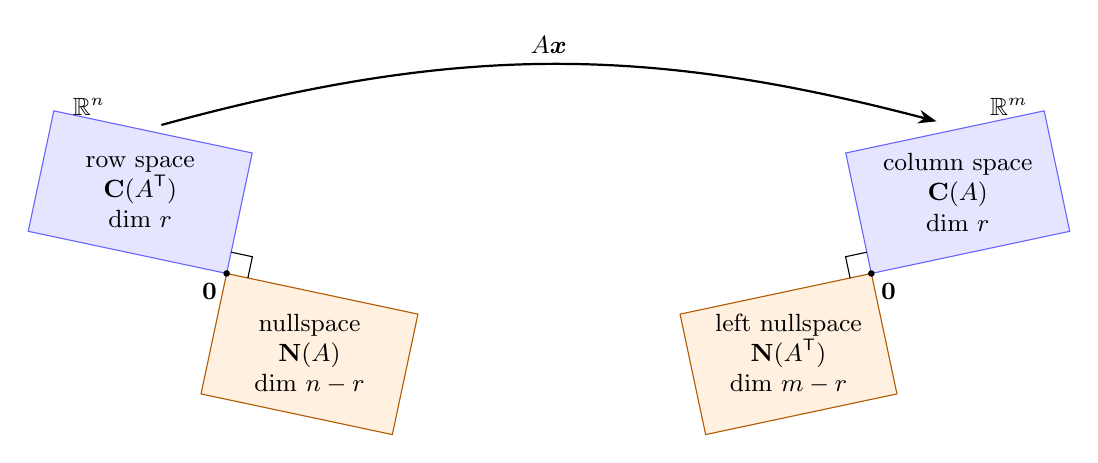
\begin{tikzpicture}[>=Stealth,font=\small,scale=0.92]
    \begin{scope}[rotate=-12]
      \filldraw[fill=blue!10,draw=blue!60] (0,0) rectangle (-2.8,1.7);
      \filldraw[fill=orange!12,draw=orange!70!black] (0,0) rectangle (2.7,-1.7);
      \draw (0,0.3) -- (0.3,0.3) -- (0.3,0);
      \node[align=center] at (-1.4,0.85) {row space\\ $\Col{A\T}$\\ dim $r$};
      \node[align=center] at (1.35,-0.85) {nullspace\\ $\Nul{A}$\\ dim $n-r$};
      \fill (0,0) circle (1.3pt) node[below left] {$\vb{0}$};
    \end{scope}
    \node at (-1.9,2.3) {$\R^n$};
    \begin{scope}[xshift=8.9cm,rotate=12]
      \filldraw[fill=blue!10,draw=blue!60] (0,0) rectangle (2.8,1.7);
      \filldraw[fill=orange!12,draw=orange!70!black] (0,0) rectangle (-2.7,-1.7);
      \draw (0,0.3) -- (-0.3,0.3) -- (-0.3,0);
      \node[align=center] at (1.4,0.85) {column space\\ $\Col{A}$\\ dim $r$};
      \node[align=center] at (-1.35,-0.85) {left nullspace\\ $\Nul{A\T}$\\ dim $m-r$};
      \fill (0,0) circle (1.3pt) node[below right] {$\vb{0}$};
    \end{scope}
    \node at (10.8,2.3) {$\R^m$};
    \draw[->,thick] (-0.9,2.05) to[bend left=15] node[above] {$A\vb{x}$} (9.8,2.1);
  \end{tikzpicture}
  \caption{The four subspaces with their right angles. In $\R^n$ the row space and nullspace
  are orthogonal complements (dimensions $r+(n-r)=n$); in $\R^m$ the column space and left
  nullspace are (dimensions $r+(m-r)=m$). Every $A\vb{x}$ lands in the column space.}
  \label{fig:u16-bigpicture}
\end{figure}

\begin{example}[A plane perpendicular to a row]\label{ex:u16-plane}
Take $A=\begin{bmatrix}1&2&5\\2&4&10\end{bmatrix}$. Row~2 is twice row~1, so $r=1$ and the
row space is the line through $(1,2,5)$. The nullspace has dimension $3-1=2$: it is the plane
$x_1+2x_2+5x_3=0$, with special solutions $(-2,1,0)$ and $(-5,0,1)$. Both are orthogonal to
$(1,2,5)$: $-2+2+0=0$ and $-5+0+5=0$. The second row adds nothing; the nullspace is the plane
whose normal vector is $(1,2,5)$, exactly as in calculus. Notice what cannot happen: the row
space and nullspace of a matrix with three columns can never be two perpendicular
\emph{lines} in $\R^3$, because their dimensions must add to $3$.
\end{example}

\begin{example}[Finding \texorpdfstring{$S^{\perp}$}{the complement} in \texorpdfstring{$\R^4$}{R4}]\label{ex:u16-sperp}
Let $S=\Span\{(1,2,2,3),\,(1,3,3,2)\}$. A vector $\vb{x}$ is in $S^{\perp}$ when it is
orthogonal to both spanning vectors (Lemma~\ref{lem:u16-span}), that is, when
$\vb{x}\in\Nul{B}$ for the matrix $B$ with those vectors as rows. Elimination subtracts row~1
from row~2:
\[
  B=\begin{bmatrix}1&2&2&3\\1&3&3&2\end{bmatrix}\longrightarrow
  \begin{bmatrix}1&2&2&3\\0&1&1&-1\end{bmatrix}.
\]
The rank is $2$, so $\dim S^{\perp}=4-2=2$. With $x_3=a$ and $x_4=b$ free, row~2 gives
$x_2=-a+b$ and row~1 gives $x_1=-2x_2-2x_3-3x_4=-5b$. Hence
\[
  \vb{x}=a\begin{bmatrix}0\\-1\\1\\0\end{bmatrix}+b\begin{bmatrix}-5\\1\\0\\1\end{bmatrix},
\]
and $(0,-1,1,0)$, $(-5,1,0,1)$ form a basis for $S^{\perp}$ (check: each has zero dot product
with both rows of $B$). By Corollary~\ref{cor:u16-split} the four vectors together are a basis
of $\R^4$ (the $4\times 4$ matrix with them as columns has determinant $53\neq 0$), so every
$\vb{v}\in\R^4$ splits uniquely into a piece of $S$ plus a piece of $S^{\perp}$.
\end{example}

\begin{example}[The left nullspace of a tall matrix]\label{ex:u16-short}
The matrix of the best-fit problem in Sections~\ref{sec:u17} and~\ref{sec:u18} is
\[
  A=\begin{bmatrix}1&0\\1&1\\1&2\end{bmatrix}.
\]
Its column space is a plane in $\R^3$ (the columns are independent), so its orthogonal
complement $\Nul{A\T}$ is a line. Solving $A\T\vb{y}=\vb{0}$, i.e.\ $y_1+y_2+y_3=0$ and
$y_2+2y_3=0$, gives $y_2=-2y_3$, $y_1=y_3$: the line through $(1,-2,1)$. Indeed
$(1,-2,1)\cdot(1,1,1)=0$ and $(1,-2,1)\cdot(0,1,2)=0$. Any $\vb{b}\in\R^3$ that is not in the
plane has a nonzero component along this line; that component will be the error vector
of least squares.
\end{example}

\subsection{The matrix \texorpdfstring{$A\T A$}{A-transpose-A}}

The main problem of this part of the course is to solve $A\vb{x}=\vb{b}$ ``as well as
possible'' when it has no solution. This is the normal situation for a tall matrix: a
satellite's position measured a thousand times gives a thousand equations in a handful of
unknowns, and noise in $\vb{b}$ pushes it off the column space. Throwing away equations until
the system is square discards information; we want to use every measurement. The equation that
does this, derived in Section~\ref{sec:u17}, is
\[
  A\T A\,\hat{\vb{x}}=A\T\vb{b}.
\]
Whatever $A$ is, $A\T A$ is square ($n\times n$) and symmetric, since
$(A\T A)\T=A\T(A\T)\T=A\T A$. The question is when it is invertible.

\begin{theorem}[\texorpdfstring{$A\T A$}{A-transpose-A} has the same nullspace as \texorpdfstring{$A$}{A}]\label{thm:u16-ata}
For every $m\times n$ matrix $A$: $\ \Nul{A\T A}=\Nul{A}$ and $\rank(A\T A)=\rank A$.
Consequently $A\T A$ is invertible if and only if the columns of $A$ are independent.
\end{theorem}

\begin{proof}
If $A\vb{x}=\vb{0}$ then $A\T A\vb{x}=\vb{0}$. Conversely, suppose $A\T A\vb{x}=\vb{0}$ and
multiply on the left by $\vb{x}\T$:
\[
  0=\vb{x}\T A\T A\vb{x}=(A\vb{x})\T(A\vb{x})=\|A\vb{x}\|^2 ,
\]
so $A\vb{x}=\vb{0}$. Equal nullspaces in $\R^n$ give equal ranks, $n-\dim\Nul{A}$. The square
matrix $A\T A$ is invertible exactly when its nullspace is $\{\vb{0}\}$, that is, when
$\Nul{A}=\{\vb{0}\}$, which means the columns of $A$ are independent.
\end{proof}

\begin{example}[Invertible and singular \texorpdfstring{$A\T A$}{A-transpose-A}]\label{ex:u16-ata}
For $A=\begin{bmatrix}1&1\\1&2\\1&5\end{bmatrix}$ the columns are independent and
\[
  A\T A=\begin{bmatrix}1&1&1\\1&2&5\end{bmatrix}\begin{bmatrix}1&1\\1&2\\1&5\end{bmatrix}
  =\begin{bmatrix}3&8\\8&30\end{bmatrix},
\]
which is invertible ($3\cdot 30-8\cdot 8=26\neq 0$). Changing the second column to $(3,3,3)$
makes the rank $1$, and then $A\T A=\begin{bmatrix}3&9\\9&27\end{bmatrix}$ has rank $1$ as
well: the vector $(3,-1)$ is in the nullspace of both $A$ and $A\T A$. For the matrix of
Example~\ref{ex:u16-short}, $A\T A=\begin{bmatrix}3&3\\3&5\end{bmatrix}$, invertible as the
theorem promises.
\end{example}

\begin{trap}
Orthogonality of subspaces is much stronger than meeting only at $\vb{0}$. And
``perpendicular'' planes in the everyday sense, like a wall and the floor, are not orthogonal
subspaces. When you test $S\perp T$, test every spanning vector of $S$ against every
spanning vector of $T$; when you claim $T=S^{\perp}$, also check that the dimensions add up
to $n$.
\end{trap}

\subsection{Exercises}

\begin{exercise}[Fredholm's alternative]\label{ex:u16-fredholm}
Exactly one of these problems has a solution: $A\vb{x}=\vb{b}$, or $A\T\vb{y}=\vb{0}$ with
$\vb{y}\T\vb{b}=1$. (If $\vb{b}\notin\Col{A}$, then $\vb{b}$ is not orthogonal to
$\Nul{A\T}$.) Multiply the equations $x_1-x_2=1$, $x_2-x_3=1$, $x_1-x_3=1$ by numbers
$y_1,y_2,y_3$ chosen so that the equations add up to $0=1$.
\end{exercise}

\begin{solution}
Take $y_1=1$, $y_2=1$, $y_3=-1$. The left sides add to
$(x_1-x_2)+(x_2-x_3)-(x_1-x_3)=0$, while the right sides add to $1+1-1=1$. So the system
implies $0=1$ and has no solution. In matrix language $\vb{y}=(1,1,-1)$ satisfies
$A\T\vb{y}=\vb{0}$ (it is in the left nullspace) and $\vb{y}\T\vb{b}=1\neq 0$, so $\vb{b}$ is
not orthogonal to $\Nul{A\T}$ and therefore not in $\Col{A}=\Nul{A\T}^{\perp}$.
\end{solution}

\begin{exercise}\label{ex:u16-four}
You are given four nonzero vectors $\vb{r},\vb{n},\vb{c},\vb{l}$ in $\R^2$.
(a) What conditions must they satisfy to be bases for $\Col{A\T}$, $\Nul{A}$, $\Col{A}$,
$\Nul{A\T}$ of some $2\times 2$ matrix $A$? (b) Give one such matrix.
\end{exercise}

\begin{solution}
(a) Each subspace has a one-vector basis, so all four have dimension $1$ and $r=1$; the
dimension counts $1+1=2$ hold automatically. What remains is orthogonality:
$\vb{r}\T\vb{n}=0$ and $\vb{c}\T\vb{l}=0$. These are also sufficient, by part (b).
(b) Take $A=\vb{c}\,\vb{r}\T$. Every column is a multiple of $\vb{c}$ and every row a multiple
of $\vb{r}$, so $\Col{A}$ is the line through $\vb{c}$ and $\Col{A\T}$ the line through
$\vb{r}$. The nullspaces are then the orthogonal complements, the lines through $\vb{n}$ and
$\vb{l}$ (Theorem~\ref{thm:u16-complements}).
\end{solution}

\begin{exercise}\label{ex:u16-impossible}
Is there a matrix whose row space contains $(1,2,1)$ and whose nullspace contains
$(1,-2,1)$?
\end{exercise}

\begin{solution}
No. The row space and the nullspace are orthogonal (Theorem~\ref{thm:u16-rowperp}), but
$(1,2,1)\cdot(1,-2,1)=1-4+1=-2\neq 0$.
\end{solution}

\begin{exercise}\label{ex:u16-splitb}
For $A=\begin{bmatrix}1&0\\1&1\\1&2\end{bmatrix}$ (Example~\ref{ex:u16-short}), split
$\vb{b}=(6,0,0)$ into a vector in $\Col{A}$ plus a vector in $\Nul{A\T}$.
\end{exercise}

\begin{solution}
$\Nul{A\T}$ is the line through $\vb{n}=(1,-2,1)$. Write $\vb{b}=\vb{p}+t\vb{n}$ with
$\vb{p}\in\Col{A}$; dotting with $\vb{n}$ kills $\vb{p}$ (Theorem~\ref{thm:u16-rowperp}), so
$\vb{n}\T\vb{b}=t\,\vb{n}\T\vb{n}$, i.e.\ $6=6t$ and $t=1$. Hence the left-nullspace part is
$(1,-2,1)$ and $\vb{p}=\vb{b}-(1,-2,1)=(5,2,-1)$. Check that $\vb{p}$ really is in the column
space: $5(1,1,1)-3(0,1,2)=(5,2,-1)$. This is the projection computed again in
Sections~\ref{sec:u17} and~\ref{sec:u18}.
\end{solution}

% unit: u17
% sources: sources/096-projections-onto-subspaces.txt, sources/028-lecture-15-projections-onto-subspaces.txt, sources/176-mit18-06scf11-ses2-2sum-pdf-download-file.txt, sources/029-problem-solving-projection-onto-subspaces.txt, sources/177-mit18-06scf11-ses2-2prob-pdf-download-file.txt, sources/178-mit18-06scf11-ses2-2sol-pdf-download-file.txt
\section{Projections onto subspaces}\label{sec:u17}

Section~\ref{sec:u16} showed that $\R^m$ splits into the column space of $A$ and the left
nullspace, at right angles. Projection makes that split computable: given $\vb{b}$, find the
point $\vb{p}$ of a subspace closest to $\vb{b}$. The answer is pinned down by a single right
angle, the error $\vb{e}=\vb{b}-\vb{p}$ must be perpendicular to the subspace, and it leads to
three formulas to remember: the coefficients $\hat{\vb{x}}$, the projection $\vb{p}$, and the
projection matrix $P$. We do the one-dimensional case first and then repeat every step for a
subspace of any dimension.

\subsection{Projecting onto a line}

Let $\vb{a}\neq\vb{0}$ and $\vb{b}$ be vectors in $\R^m$. The point of the line through
$\vb{a}$ closest to $\vb{b}$ is some multiple $\vb{p}=\hat{x}\,\vb{a}$. Trigonometry would
express $\hat{x}$ with $\cos\theta$; linear algebra only needs the right angle in
Figure~\ref{fig:u17-line}: the error $\vb{e}=\vb{b}-\hat{x}\vb{a}$ is perpendicular to
$\vb{a}$.
\[
  \vb{a}\T(\vb{b}-\hat{x}\vb{a})=0
  \quad\Longrightarrow\quad
  \hat{x}\,\vb{a}\T\vb{a}=\vb{a}\T\vb{b}
  \quad\Longrightarrow\quad
  \hat{x}=\frac{\vb{a}\T\vb{b}}{\vb{a}\T\vb{a}},\qquad
  \vb{p}=\vb{a}\,\frac{\vb{a}\T\vb{b}}{\vb{a}\T\vb{a}} .
\]
Two sanity checks: doubling $\vb{b}$ doubles $\vb{p}$; doubling $\vb{a}$ (or replacing it by
$-\vb{a}$) does not change $\vb{p}$, because the line is the same: replacing $\vb{a}$ by $2\vb{a}$ multiplies the
numerator and the denominator by $4$.

\begin{figure}[ht]
  \centering
  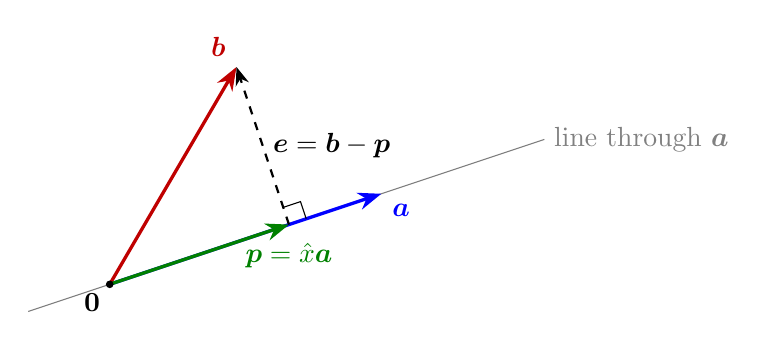
\begin{tikzpicture}[>=Stealth,scale=1.15]
    \draw[gray] (-0.9,-0.3) -- (4.8,1.6) node[right] {line through $\vb{a}$};
    \draw[->,very thick,blue] (0,0) -- (3,1) node[below right] {$\vb{a}$};
    \draw[->,very thick,red!75!black] (0,0) -- (1.4,2.4) node[above left] {$\vb{b}$};
    \draw[->,very thick,green!50!black] (0,0) -- (1.98,0.66) node[below=3pt] {$\vb{p}=\hat{x}\vb{a}$};
    \draw[->,thick,dashed] (1.98,0.66) -- (1.4,2.4) node[midway,right] {$\vb{e}=\vb{b}-\vb{p}$};
    \draw[shift={(1.98,0.66)},rotate=18.43] (0.2,0) -- (0.2,0.2) -- (0,0.2);
    \fill (0,0) circle (1.2pt) node[below left] {$\vb{0}$};
  \end{tikzpicture}
  \caption{Projection onto a line. The closest point $\vb{p}$ is where the perpendicular from
  $\vb{b}$ meets the line; the error $\vb{e}$ is orthogonal to $\vb{a}$, which is the equation
  $\vb{a}\T(\vb{b}-\hat{x}\vb{a})=0$.}
  \label{fig:u17-line}
\end{figure}

\begin{proposition}[The perpendicular foot is closest]\label{prop:u17-closest-line}
For every number $t$,
$\ \|\vb{b}-t\vb{a}\|^2=\|\vb{e}\|^2+(t-\hat{x})^2\|\vb{a}\|^2$. Hence $\vb{p}=\hat{x}\vb{a}$
is the unique point of the line closest to $\vb{b}$.
\end{proposition}

\begin{proof}
Write $\vb{b}-t\vb{a}=\vb{e}+(\hat{x}-t)\vb{a}$. The two pieces are orthogonal, so
Pythagoras (Section~\ref{sec:u16}) adds their squared lengths. The second term is zero only for $t=\hat{x}$.
\end{proof}

The projection is a linear function of $\vb{b}$, so a matrix does it. Moving the parentheses
in $\vb{p}=\vb{a}(\vb{a}\T\vb{b})/(\vb{a}\T\vb{a})$ gives $\vb{p}=P\vb{b}$ with:

\begin{definition}[Projection matrix onto a line]\label{def:u17-pline}
The matrix that projects onto the line through $\vb{a}\in\R^m$ is the $m\times m$ matrix
\[
  P=\frac{\vb{a}\vb{a}\T}{\vb{a}\T\vb{a}} .
\]
The numerator is a column times a row, a full matrix; the denominator is a number.
\end{definition}

\begin{proposition}\label{prop:u17-pline-props}
The matrix $P=\vb{a}\vb{a}\T/\vb{a}\T\vb{a}$ has column space the line through $\vb{a}$, rank
$1$, and satisfies $P\T=P$ and $P^2=P$.
\end{proposition}

\begin{proof}
$P\vb{b}$ is always a multiple of $\vb{a}$, and $P\vb{a}=\vb{a}$, so $\Col{P}$ is the line
through $\vb{a}$ and the rank is $1$. Transposing, $(\vb{a}\vb{a}\T)\T=\vb{a}\vb{a}\T$, so
$P\T=P$. Finally
$P^2=\vb{a}(\vb{a}\T\vb{a})\vb{a}\T/(\vb{a}\T\vb{a})^2=\vb{a}\vb{a}\T/\vb{a}\T\vb{a}=P$:
projecting a second time leaves a point already on the line where it is.
\end{proof}

\begin{example}[Projecting onto the line through \texorpdfstring{$(1,2,2)$}{(1,2,2)}]\label{ex:u17-line}
Let $\vb{a}=(1,2,2)$ and $\vb{b}=(1,1,1)$. Then $\vb{a}\T\vb{b}=5$ and $\vb{a}\T\vb{a}=9$, so
\[
  \hat{x}=\tfrac{5}{9},\qquad
  \vb{p}=\tfrac{5}{9}(1,2,2)=\bigl(\tfrac59,\tfrac{10}9,\tfrac{10}9\bigr),\qquad
  \vb{e}=\vb{b}-\vb{p}=\bigl(\tfrac49,-\tfrac19,-\tfrac19\bigr).
\]
Check: $\vb{a}\T\vb{e}=\frac{4-2-2}{9}=0$. The projection matrix is
\[
  P=\frac{1}{9}\begin{bmatrix}1\\2\\2\end{bmatrix}\begin{bmatrix}1&2&2\end{bmatrix}
   =\frac{1}{9}\begin{bmatrix}1&2&2\\2&4&4\\2&4&4\end{bmatrix},
\]
symmetric and of rank one, and $P\vb{b}=\frac19(5,10,10)=\vb{p}$.
\end{example}

\subsection{Why project: the closest solvable problem}

The equation $A\vb{x}=\vb{b}$ may have no solution: $A\vb{x}$ always lies in $\Col{A}$, while
$\vb{b}$, typically a list of measurements with errors, does not. The natural repair is to
replace $\vb{b}$ by the closest vector $\vb{p}$ that \emph{is} in the column space and solve
$A\hat{\vb{x}}=\vb{p}$ instead. The hat on $\hat{\vb{x}}$ marks it as the best available
coefficient vector rather than an exact solution. So we need to project onto a column space.

\subsection{Projecting onto a subspace}

Let the subspace be spanned by independent vectors $\vb{a}_1,\dots,\vb{a}_n$ in $\R^m$, and
put them into the columns of the $m\times n$ matrix $A$, so the subspace is $\Col{A}$. The
columns need not be perpendicular, only independent. The projection is a combination
$\vb{p}=\hat{x}_1\vb{a}_1+\cdots+\hat{x}_n\vb{a}_n=A\hat{\vb{x}}$, and the error
$\vb{e}=\vb{b}-A\hat{\vb{x}}$ must be perpendicular to the subspace, which means
perpendicular to every column:
\[
  \vb{a}_1\T(\vb{b}-A\hat{\vb{x}})=0,\ \ \dots,\ \ \vb{a}_n\T(\vb{b}-A\hat{\vb{x}})=0
  \qquad\Longleftrightarrow\qquad
  A\T(\vb{b}-A\hat{\vb{x}})=\vb{0}.
\]
The $n$ dot products stack into one matrix equation because the rows of $A\T$ are the
columns of $A$. With one column this is the line equation $\vb{a}\T(\vb{b}-\hat{x}\vb{a})=0$
again. The equation also says $\vb{e}\in\Nul{A\T}$, which by Section~\ref{sec:u16} is
precisely the orthogonal complement of $\Col{A}$: the algebra and the geometry agree.

\begin{theorem}[Projection onto a column space]\label{thm:u17-projection}
Let $A$ be $m\times n$ with independent columns and $\vb{b}\in\R^m$. The vector
$\hat{\vb{x}}$ for which $\vb{e}=\vb{b}-A\hat{\vb{x}}$ is orthogonal to $\Col{A}$ is the unique
solution of the \emph{normal equations}
\[
  A\T A\,\hat{\vb{x}}=A\T\vb{b},
\]
and
\[
  \hat{\vb{x}}=(A\T A)^{-1}A\T\vb{b},\qquad
  \vb{p}=A\hat{\vb{x}}=A(A\T A)^{-1}A\T\vb{b},\qquad
  P=A(A\T A)^{-1}A\T .
\]
\end{theorem}

\begin{proof}
The orthogonality condition is $A\T(\vb{b}-A\hat{\vb{x}})=\vb{0}$, which rearranges to the
normal equations. Because the columns of $A$ are independent, $A\T A$ is invertible
(by $\Nul{A\T A}=\Nul{A}$, Section~\ref{sec:u16}), so the solution exists, is unique, and
equals $(A\T A)^{-1}A\T\vb{b}$. Multiplying by $A$ gives $\vb{p}$, and the matrix that
multiplies $\vb{b}$ is $P$.
\end{proof}

When $n=1$ the matrix $A\T A$ is the number $\vb{a}\T\vb{a}$ and ``divide by it'' becomes
``multiply by its inverse''; the formulas reduce to those for a line.

\begin{proposition}[Projection matrices are symmetric and idempotent]\label{prop:u17-pprops}
$P=A(A\T A)^{-1}A\T$ satisfies $P\T=P$ and $P^2=P$.
\end{proposition}

\begin{proof}
$A\T A$ is symmetric, so its inverse is symmetric too, and
$P\T=(A\T)\T\bigl((A\T A)^{-1}\bigr)\T A\T=A(A\T A)^{-1}A\T=P$. For the square, the middle
factors cancel:
\[
  P^2=A(A\T A)^{-1}\underbrace{(A\T A)(A\T A)^{-1}}_{I}A\T=A(A\T A)^{-1}A\T=P.\qedhere
\]
\end{proof}

\begin{theorem}[The projection is the closest point]\label{thm:u17-closest}
For every $\vb{x}\in\R^n$,
$\ \|\vb{b}-A\vb{x}\|^2=\|\vb{b}-\vb{p}\|^2+\|A(\hat{\vb{x}}-\vb{x})\|^2$. Hence
$\vb{p}=A\hat{\vb{x}}$ is the unique point of $\Col{A}$ closest to $\vb{b}$.
\end{theorem}

\begin{proof}
Split $\vb{b}-A\vb{x}=(\vb{b}-A\hat{\vb{x}})+A(\hat{\vb{x}}-\vb{x})=\vb{e}+A(\hat{\vb{x}}-\vb{x})$.
The second piece lies in $\Col{A}$ and $\vb{e}$ is orthogonal to $\Col{A}$, so Pythagoras
applies. The extra term vanishes only when $A\vb{x}=A\hat{\vb{x}}$, i.e.\ at $\vb{p}$.
\end{proof}

\begin{trap}
It is tempting to simplify $A(A\T A)^{-1}A\T$ to $AA^{-1}(A\T)^{-1}A\T=I$. That is only
legal when $A$ is square and invertible, and then the answer $P=I$ is correct: the column
space is all of $\R^m$ and every $\vb{b}$ is its own projection. For the tall matrices of
interest, $A$ has no inverse, $(A\T A)^{-1}$ cannot be split, and $P\neq I$.
\end{trap}

\begin{example}[Projecting \texorpdfstring{$(6,0,0)$}{(6,0,0)} onto a plane]\label{ex:u17-plane}
Project $\vb{b}=(6,0,0)$ onto the plane spanned by $\vb{a}_1=(1,1,1)$ and $\vb{a}_2=(0,1,2)$
(this is the data of the line fit in Section~\ref{sec:u18}). Here
\[
  A=\begin{bmatrix}1&0\\1&1\\1&2\end{bmatrix},\qquad
  A\T A=\begin{bmatrix}3&3\\3&5\end{bmatrix},\qquad
  A\T\vb{b}=\begin{bmatrix}6\\0\end{bmatrix}.
\]
The normal equations are $3\hat{x}_1+3\hat{x}_2=6$ and $3\hat{x}_1+5\hat{x}_2=0$. Subtracting,
$2\hat{x}_2=-6$, so $\hat{x}_2=-3$ and then $\hat{x}_1=5$. Therefore
\[
  \vb{p}=5\begin{bmatrix}1\\1\\1\end{bmatrix}-3\begin{bmatrix}0\\1\\2\end{bmatrix}
  =\begin{bmatrix}5\\2\\-1\end{bmatrix},\qquad
  \vb{e}=\vb{b}-\vb{p}=\begin{bmatrix}1\\-2\\1\end{bmatrix}.
\]
The right angle checks out: $\vb{e}\T\vb{a}_1=1-2+1=0$ and $\vb{e}\T\vb{a}_2=0-2+2=0$. With
$(A\T A)^{-1}=\frac16\left[\begin{smallmatrix}5&-3\\-3&3\end{smallmatrix}\right]$ the
projection matrix is
\[
  P=A(A\T A)^{-1}A\T=\frac16\begin{bmatrix}5&2&-1\\2&2&2\\-1&2&5\end{bmatrix},
  \qquad
  I-P=\frac16\begin{bmatrix}1&-2&1\\-2&4&-2\\1&-2&1\end{bmatrix}.
\]
$P$ is symmetric, $P\vb{b}=\frac16(30,12,-6)=(5,2,-1)$, and $I-P$ is exactly
$\vb{e}\vb{e}\T/\vb{e}\T\vb{e}$ with $\vb{e}=(1,-2,1)$: the projection onto the left
nullspace, the line through $(1,-2,1)$ found in Section~\ref{sec:u16}.
Figure~\ref{fig:u17-plane} shows the picture.
\end{example}

\begin{figure}[ht]
  \centering
  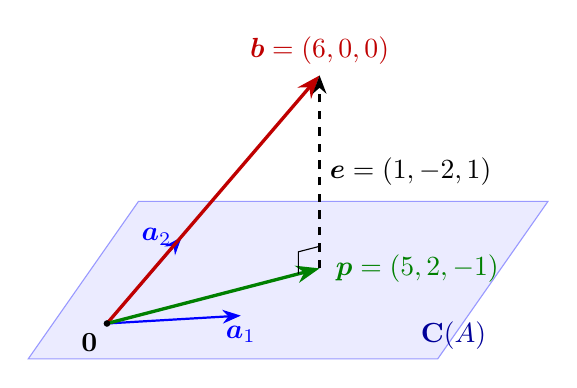
\begin{tikzpicture}[>=Stealth,scale=1.0]
    \filldraw[fill=blue!8,draw=blue!40] (0,0) -- (5.2,0) -- (6.6,2.0) -- (1.4,2.0) -- cycle;
    \node[blue!60!black] at (5.4,0.3) {$\Col{A}$};
    \coordinate (O) at (1.0,0.45);
    \coordinate (P) at (3.7,1.15);
    \coordinate (B) at (3.7,3.6);
    \draw[->,thick,blue] (O) -- (2.7,0.55) node[below] {$\vb{a}_1$};
    \draw[->,thick,blue] (O) -- (1.95,1.55) node[left] {$\vb{a}_2$};
    \draw[->,very thick,red!75!black] (O) -- (B) node[above] {$\vb{b}=(6,0,0)$};
    \draw[->,very thick,green!50!black] (O) -- (P) node[right=2pt] {$\vb{p}=(5,2,-1)$};
    \draw[->,thick,dashed] (P) -- (B) node[midway,right] {$\vb{e}=(1,-2,1)$};
    \draw (3.7,1.43) -- (3.43,1.36) -- (3.43,1.08);
    \fill (O) circle (1.2pt) node[below left] {$\vb{0}$};
  \end{tikzpicture}
  \caption{Projection onto the plane spanned by $\vb{a}_1=(1,1,1)$ and $\vb{a}_2=(0,1,2)$
  (schematic). The error $\vb{e}$ is perpendicular to the whole plane, so it lies in
  $\Nul{A\T}$; $\vb{p}$ and $\vb{e}$ add back to $\vb{b}$.}
  \label{fig:u17-plane}
\end{figure}

Different bases for the same subspace give the same $P$ (Exercise~\ref{ex:u17-basis}). This
is often useful, as in the next example: the formula needs \emph{some} basis, and the
complementary projection can be quicker.

\begin{example}[Projection onto the plane \texorpdfstring{$x+y-z=0$}{x+y-z=0}]\label{ex:u17-normal}
Two independent vectors in the plane are $(1,-1,0)$ and $(1,0,1)$. With them as columns,
\[
  A=\begin{bmatrix}1&1\\-1&0\\0&1\end{bmatrix},\qquad
  A\T A=\begin{bmatrix}2&1\\1&2\end{bmatrix},\qquad
  (A\T A)^{-1}=\frac13\begin{bmatrix}2&-1\\-1&2\end{bmatrix},
\]
and multiplying out,
\[
  P=A(A\T A)^{-1}A\T=\frac13\begin{bmatrix}2&-1&1\\-1&2&1\\1&1&2\end{bmatrix}.
\]
A quicker route: every $\vb{b}$ is its projection onto the plane plus its projection onto the
normal line through $\vb{n}=(1,1,-1)$, so $I=P+P_{\vb{n}}$ and
\[
  P=I-\frac{\vb{n}\vb{n}\T}{\vb{n}\T\vb{n}}
   =I-\frac13\begin{bmatrix}1&1&-1\\1&1&-1\\-1&-1&1\end{bmatrix}
   =\frac13\begin{bmatrix}2&-1&1\\-1&2&1\\1&1&2\end{bmatrix},
\]
the same matrix. A good final check: $P\vb{n}=\vb{0}$, since the normal vector projects to
the origin.
\end{example}

\subsection{Exercises}

\begin{exercise}\label{ex:u17-drop}
Let $A$ be the $4\times 4$ identity matrix with its last column removed, so $A$ is
$4\times 3$. Project $\vb{b}=(1,2,3,4)$ onto $\Col{A}$. What shape is $P$, and what is it?
\end{exercise}

\begin{solution}
$P$ is $4\times 4$: it takes vectors of $\R^4$ to vectors of $\R^4$. Here $A\T A=I_3$, so
$P=AA\T$, which is the identity with its last diagonal entry replaced by $0$:
\[
  P=\begin{bmatrix}1&0&0&0\\0&1&0&0\\0&0&1&0\\0&0&0&0\end{bmatrix},\qquad
  \vb{p}=P\vb{b}=(1,2,3,0).
\]
Geometrically, $\Col{A}$ is the coordinate subspace of the first three axes, and projecting
onto it just zeroes the fourth coordinate.
\end{solution}

\begin{exercise}\label{ex:u17-complement}
If $P^2=P$, show that $(I-P)^2=I-P$. For the matrices of
Exercise~\ref{ex:u17-drop}, $P$ projects onto $\Col{A}$; onto which subspace does $I-P$
project?
\end{exercise}

\begin{solution}
$(I-P)^2=I-2P+P^2=I-2P+P=I-P$. In Exercise~\ref{ex:u17-drop},
$I-P=\operatorname{diag}(0,0,0,1)$ projects onto the fourth axis, which is the left nullspace
$\Nul{A\T}$: the vectors orthogonal to the first three columns of $I$. In general $I-P$ sends
$\vb{b}$ to $\vb{e}$, the component in $\Nul{A\T}$.
\end{solution}

\begin{exercise}\label{ex:u17-basis}
Show that $P=A(A\T A)^{-1}A\T$ does not change when $A$ is replaced by $AM$ for an invertible
$n\times n$ matrix $M$ (a different basis for the same column space).
\end{exercise}

\begin{solution}
Using $(XY)^{-1}=Y^{-1}X^{-1}$ for the square invertible factors $M\T$, $A\T A$, $M$:
\begin{align*}
  AM\bigl((AM)\T AM\bigr)^{-1}(AM)\T
  &=AM\bigl(M\T(A\T A)M\bigr)^{-1}M\T A\T\\
  &=AM\,M^{-1}(A\T A)^{-1}(M\T)^{-1}M\T A\T
  =A(A\T A)^{-1}A\T .
\end{align*}
So $P$ depends only on the subspace, as the geometry demands. This is why the two
different bases in Example~\ref{ex:u17-normal} could not have given different answers.
\end{solution}

% unit: u18
% sources: sources/097-projection-matrices-and-least-squares.txt, sources/030-lecture-16-projection-matrices-and-least-squares.txt, sources/179-mit18-06scf11-ses2-3sum-pdf-download-file.txt, sources/031-problem-solving-least-squares-approximation.txt, sources/180-mit18-06scf11-ses2-3prob-pdf-download-file.txt, sources/181-mit18-06scf11-ses2-3sol-pdf-download-file.txt
\section{Projection matrices and least squares}\label{sec:u18}

This section puts the projection formulas of Section~\ref{sec:u17} to work on their most
important application: fitting a straight line to data that no line passes through exactly.
First we look once more at what $P=A(A\T A)^{-1}A\T$ does to the two kinds of vectors it can
meet, because that explains the whole least-squares picture: $\vb{b}$ splits into a part
$\vb{p}$ that the model can explain and an error $\vb{e}$ that it cannot, at right angles.

\subsection{What a projection does to \texorpdfstring{$\vb{b}$}{b}}

\begin{proposition}[The two extreme cases]\label{prop:u18-extremes}
Let $A$ have independent columns and $P=A(A\T A)^{-1}A\T$.
If $\vb{b}\in\Col{A}$ then $P\vb{b}=\vb{b}$; if $\vb{b}\in\Nul{A\T}$ (perpendicular to the
column space) then $P\vb{b}=\vb{0}$.
\end{proposition}

\begin{proof}
A vector in the column space has the form $\vb{b}=A\vb{x}$, and then
$P\vb{b}=A(A\T A)^{-1}(A\T A)\vb{x}=A\vb{x}=\vb{b}$. A vector in $\Nul{A\T}$ has
$A\T\vb{b}=\vb{0}$, and the last factor of $P$ kills it.
\end{proof}

A typical $\vb{b}$ is neither: it has a component in $\Col{A}$ and a component in $\Nul{A\T}$
(Section~\ref{sec:u16}), and the projection keeps the first and kills the second.

\begin{proposition}[The complementary projection]\label{prop:u18-iminusp}
$I-P$ is the projection matrix onto $\Nul{A\T}$: it is symmetric, $(I-P)^2=I-P$, and
$\vb{b}=P\vb{b}+(I-P)\vb{b}=\vb{p}+\vb{e}$ with $\vb{p}\in\Col{A}$, $\vb{e}\in\Nul{A\T}$.
\end{proposition}

\begin{proof}
$(I-P)\T=I-P\T=I-P$, and $(I-P)^2=I-2P+P^2=I-P$ because $P^2=P$. The vector
$(I-P)\vb{b}=\vb{b}-A\hat{\vb{x}}=\vb{e}$ satisfies $A\T\vb{e}=\vb{0}$ by the normal equations,
so it lies in $\Nul{A\T}$. By Proposition~\ref{prop:u18-extremes}, $I-P$ fixes vectors of
$\Nul{A\T}$ and kills vectors of $\Col{A}$; so it is the projection onto $\Nul{A\T}$.
\end{proof}

\subsection{Fitting a line: the least-squares problem}

We are given three measurements $(t,b)=(1,1),\,(2,2),\,(3,2)$ and want the line $b=C+Dt$
that comes closest. If the line went through all three points we would have
\[
  \begin{aligned}
    C+D&=1\\ C+2D&=2\\ C+3D&=2
  \end{aligned}
  \qquad\text{i.e.}\qquad
  \underbrace{\begin{bmatrix}1&1\\1&2\\1&3\end{bmatrix}}_{A}
  \underbrace{\begin{bmatrix}C\\D\end{bmatrix}}_{\vb{x}}
  =\underbrace{\begin{bmatrix}1\\2\\2\end{bmatrix}}_{\vb{b}} .
\]
The first two equations force $C=0$, $D=1$, and then the third fails ($3\neq 2$). Three
equations, two unknowns, no solution: $\vb{b}$ is not in the plane $\Col{A}$. Any choice of
$C,D$ misses by the vector $A\vb{x}-\vb{b}$, whose components are the misses at the three data
points.

\begin{definition}[Least-squares solution]\label{def:u18-ls}
A \emph{least-squares solution} of $A\vb{x}=\vb{b}$ is a vector $\hat{\vb{x}}$ that minimizes
the total squared error
\[
  E(\vb{x})=\|A\vb{x}-\vb{b}\|^2=e_1^2+e_2^2+\cdots+e_m^2 .
\]
Fitting a line this way is called \emph{linear regression}.
\end{definition}

There are two pictures of the same computation, and it pays to keep both. In the
\emph{data picture} ($t$ horizontal, $b$ vertical) the errors $e_i$ are the \emph{vertical}
distances from the data points to the line, and $p_i=C+Dt_i$ are the heights of the line
above the $t_i$. In the \emph{vector picture} in $\R^m$, $\vb{b}$ is one vector, the line
corresponds to a point $\vb{p}=A\hat{\vb{x}}$ of the column space, and
$\vb{e}=\vb{b}-\vb{p}$ is the perpendicular from $\vb{b}$ to that plane. The second picture
tells us how to minimize.

\begin{theorem}[Least squares = projection]\label{thm:u18-ls}
If $A$ has independent columns, the unique least-squares solution of $A\vb{x}=\vb{b}$ is the
solution of the normal equations $A\T A\hat{\vb{x}}=A\T\vb{b}$. The best fit is
$\vb{p}=A\hat{\vb{x}}=P\vb{b}$, the minimum squared error is $\|\vb{e}\|^2$ with
$\vb{e}=\vb{b}-\vb{p}$, and $\vb{e}$ is orthogonal to every column of $A$.
\end{theorem}

\begin{proof}
For any $\vb{x}$,
$A\vb{x}-\vb{b}=A(\vb{x}-\hat{\vb{x}})-\vb{e}$, where $A(\vb{x}-\hat{\vb{x}})\in\Col{A}$ and
$\vb{e}\in\Nul{A\T}$ is orthogonal to it. By Pythagoras,
\[
  \|A\vb{x}-\vb{b}\|^2=\|A(\vb{x}-\hat{\vb{x}})\|^2+\|\vb{e}\|^2\ \ge\ \|\vb{e}\|^2 ,
\]
with equality only when $A(\vb{x}-\hat{\vb{x}})=\vb{0}$, which (independent columns) means
$\vb{x}=\hat{\vb{x}}$.
\end{proof}

Calculus reaches the same equations. For the three points above,
\[
  E(C,D)=(C+D-1)^2+(C+2D-2)^2+(C+3D-2)^2 ,
\]
and setting both partial derivatives to zero gives
\[
  \tfrac12\tfrac{\partial E}{\partial C}=3C+6D-5=0,\qquad
  \tfrac12\tfrac{\partial E}{\partial D}=6C+14D-11=0,
\]
which are exactly the normal equations below. In general the gradient of $\|A\vb{x}-\vb{b}\|^2$
is $2A\T(A\vb{x}-\vb{b})$, and setting it to zero is $A\T A\vb{x}=A\T\vb{b}$. Because the
error is a sum of \emph{squares}, its derivatives are linear, which is why the minimum comes
from a linear system.

\begin{example}[The lecture's line through \texorpdfstring{$(1,1),(2,2),(3,2)$}{three points}]\label{ex:u18-lecture}
Compute
\[
  A\T A=\begin{bmatrix}1&1&1\\1&2&3\end{bmatrix}\begin{bmatrix}1&1\\1&2\\1&3\end{bmatrix}
  =\begin{bmatrix}3&6\\6&14\end{bmatrix},\qquad
  A\T\vb{b}=\begin{bmatrix}1+2+2\\1+4+6\end{bmatrix}=\begin{bmatrix}5\\11\end{bmatrix}.
\]
The matrix is symmetric and invertible, as Section~\ref{sec:u16} promised. Elimination:
subtract twice the first equation $3\hat C+6\hat D=5$ from the second $6\hat C+14\hat D=11$ to
get $2\hat D=1$, so $\hat D=\tfrac12$; back substitution gives $3\hat C+3=5$, so
$\hat C=\tfrac23$. The best line is
\[
  b=\tfrac23+\tfrac12 t .
\]
Its heights at $t=1,2,3$ and the errors are
\[
  \vb{p}=\begin{bmatrix}7/6\\5/3\\13/6\end{bmatrix},\qquad
  \vb{e}=\vb{b}-\vb{p}=\begin{bmatrix}-1/6\\1/3\\-1/6\end{bmatrix},
\]
and indeed $\vb{p}+\vb{e}=\vb{b}$. Three checks of the geometry:
$\vb{p}\T\vb{e}=\frac{-7+20-13}{36}=0$;
$\vb{e}\T(1,1,1)=-\frac16+\frac13-\frac16=0$; and
$\vb{e}\T(1,2,3)=\frac{-1+4-3}{6}=0$. The error is perpendicular not only to $\vb{p}$ but to
the whole column space. The minimum total squared error is
$\|\vb{e}\|^2=\frac{1+4+1}{36}=\frac16$.
\end{example}

\subsection{The best line leaves a perpendicular error}

The following example is the one worked in the short video for this part of the course.

\begin{example}[Fitting \texorpdfstring{$(0,6),(1,0),(2,0)$}{three points}]\label{ex:u18-short}
Fit $b=C+Dt$ to the points $(t,b)=(0,6),\,(1,0),\,(2,0)$. Here
\[
  A=\begin{bmatrix}1&0\\1&1\\1&2\end{bmatrix},\qquad
  \vb{x}=\begin{bmatrix}C\\D\end{bmatrix},\qquad
  \vb{b}=\begin{bmatrix}6\\0\\0\end{bmatrix}.
\]
\emph{No exact line.} The point at $t=0$ forces $C=6$. Then $C+D=0$ needs $D=-6$, but
$C+2D=0$ needs $D=-3$: contradiction.

\emph{Normal equations.}
$A\T A=\begin{bmatrix}3&3\\3&5\end{bmatrix}$ and $A\T\vb{b}=(6,0)$, so
\[
  3C+3D=6,\qquad 3C+5D=0 .
\]
Subtracting, $2D=-6$, so $D=-3$ and $C=5$. The best line is $b=5-3t$.

\emph{Projection and error.} The line's heights at $t=0,1,2$ are $\vb{p}=(5,2,-1)$, so the
errors are $\vb{e}=\vb{b}-\vb{p}=(1,-2,1)$: the first and last points sit $1$ above the line,
the middle one $2$ below (Figure~\ref{fig:u18-fits}, right).

\emph{Right-angle check.} $\vb{e}\T(1,1,1)=1-2+1=0$ and $\vb{e}\T(0,1,2)=0-2+2=0$. The error
is perpendicular to both columns, i.e.\ $\vb{e}\in\Nul{A\T}$, the line through $(1,-2,1)$ found
in Section~\ref{sec:u16}.

\emph{Result.} The total squared error is $1+4+1=6$. For comparison, the line $b=6-3t$
through the first point has errors $(0,-3,0)$ and squared error $9$, and the horizontal line
$b=2$ (the mean of the data) has errors $(4,-2,-2)$ and squared error $24$. The vector
picture of this fit, with $\vb{b}=(6,0,0)$ dropping perpendicularly onto the plane of the
columns, is drawn in Section~\ref{sec:u17}.
\end{example}

\begin{figure}[ht]
  \centering
  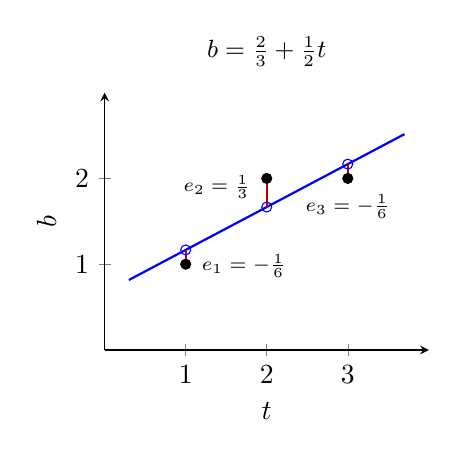
\begin{tikzpicture}
    \begin{axis}[width=0.47\textwidth,height=0.4\textwidth,xmin=0,xmax=4,ymin=0,ymax=3,
        xlabel={$t$},ylabel={$b$},axis lines=left,xtick={1,2,3},ytick={1,2},
        title={\small $b=\tfrac23+\tfrac12t$},clip=false]
      \addplot[thick,blue,domain=0.3:3.7] {2/3+x/2};
      \draw[red!75!black,thick] (axis cs:1,1) -- (axis cs:1,7/6);
      \draw[red!75!black,thick] (axis cs:2,2) -- (axis cs:2,5/3);
      \draw[red!75!black,thick] (axis cs:3,2) -- (axis cs:3,13/6);
      \addplot[only marks,mark=*,mark size=1.8pt] coordinates {(1,1) (2,2) (3,2)};
      \addplot[only marks,mark=o,mark size=1.8pt,blue] coordinates {(1,7/6) (2,5/3) (3,13/6)};
      \node[anchor=west,font=\scriptsize] at (axis cs:1.08,0.98) {$e_1=-\tfrac16$};
      \node[anchor=east,font=\scriptsize] at (axis cs:1.92,1.9) {$e_2=\tfrac13$};
      \node[anchor=north,font=\scriptsize] at (axis cs:3,1.92) {$e_3=-\tfrac16$};
    \end{axis}
  \end{tikzpicture}\hfill
  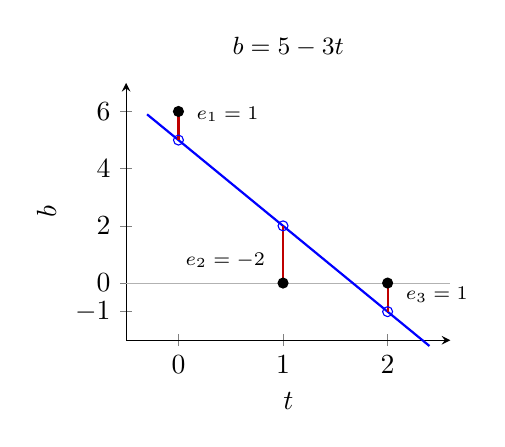
\begin{tikzpicture}
    \begin{axis}[width=0.47\textwidth,height=0.4\textwidth,xmin=-0.5,xmax=2.6,ymin=-2,ymax=7,
        xlabel={$t$},ylabel={$b$},axis lines=left,xtick={0,1,2},ytick={-1,0,2,4,6},
        title={\small $b=5-3t$},clip=false]
      \draw[gray!60] (axis cs:-0.5,0) -- (axis cs:2.6,0);
      \addplot[thick,blue,domain=-0.3:2.4] {5-3*x};
      \draw[red!75!black,thick] (axis cs:0,6) -- (axis cs:0,5);
      \draw[red!75!black,thick] (axis cs:1,0) -- (axis cs:1,2);
      \draw[red!75!black,thick] (axis cs:2,0) -- (axis cs:2,-1);
      \addplot[only marks,mark=*,mark size=1.8pt] coordinates {(0,6) (1,0) (2,0)};
      \addplot[only marks,mark=o,mark size=1.8pt,blue] coordinates {(0,5) (1,2) (2,-1)};
      \node[anchor=west,font=\scriptsize] at (axis cs:0.08,5.9) {$e_1=1$};
      \node[anchor=east,font=\scriptsize] at (axis cs:0.92,0.8) {$e_2=-2$};
      \node[anchor=west,font=\scriptsize] at (axis cs:2.08,-0.4) {$e_3=1$};
    \end{axis}
  \end{tikzpicture}
  \caption{The data picture of two least-squares fits. Dots are the data $b_i$, circles the
  heights $p_i$ of the best line, red segments the vertical errors $e_i=b_i-p_i$. Left: the
  lecture's points; right: the points $(0,6),(1,0),(2,0)$ with errors $(1,-2,1)$. The right
  angle of least squares is not visible here; it lives in $\R^3$, between $\vb{e}$ and the
  column space.}
  \label{fig:u18-fits}
\end{figure}

\begin{trap}
Least squares does \emph{not} minimize the perpendicular distances from the points to the
line. It minimizes the sum of squared \emph{vertical} errors $e_i=b_i-(C+Dt_i)$, because those
are the components of $A\vb{x}-\vb{b}$. The right angle is between $\vb{e}$ and $\Col{A}$ in
$\R^m$, not between the error segments and the line in the $t$--$b$ plane. A second warning:
squaring makes a single wild measurement (an \emph{outlier}) count heavily, so one bad point can
swing the whole line; statisticians check for outliers before trusting a least-squares fit.
\end{trap}

\subsection{When the normal equations can be solved}

Everything above assumed that $A\T A$ is invertible.

\begin{theorem}\label{thm:u18-invertible}
If $A$ has independent columns, then $A\T A$ is invertible.
\end{theorem}

\begin{proof}
Suppose $A\T A\vb{x}=\vb{0}$; we show $\vb{x}=\vb{0}$. Multiply by $\vb{x}\T$:
$\vb{x}\T A\T A\vb{x}=(A\vb{x})\T(A\vb{x})=\|A\vb{x}\|^2=0$, so $A\vb{x}=\vb{0}$. Independent
columns mean the only solution of $A\vb{x}=\vb{0}$ is $\vb{x}=\vb{0}$. So $\Nul{A\T A}=\{\vb{0}\}$
and the square matrix $A\T A$ is invertible. (This is half of the equality
$\Nul{A\T A}=\Nul{A}$ of Section~\ref{sec:u16}.)
\end{proof}

For a line fit, the columns $(1,\dots,1)$ and $(t_1,\dots,t_m)$ are independent as soon as two
of the $t_i$ differ, so least squares always has a unique line unless all measurements are at
the same time. Columns are certainly independent when they are \emph{orthonormal}:
perpendicular unit vectors such as $(1,0,0),(0,1,0),(0,0,1)$, or $(\cos\theta,\sin\theta)$ and
$(-\sin\theta,\cos\theta)$. Then $A\T A=I$ and the normal equations need no solving at all.
Section~\ref{sec:u19} shows how to make the columns orthonormal.

Nothing in the method needs the model to be a straight line; it only needs the unknown
coefficients to enter \emph{linearly}. A parabola $C+Dt+Et^2$ gives a matrix with columns $1$,
$t_i$, $t_i^2$; a curve through the origin $ct+dt^2$ gives columns $t_i$ and $t_i^2$
(Exercise~\ref{ex:u18-quad}).

\subsection{Exercises}

\begin{exercise}\label{ex:u18-ex1}
Write down three equations for the line $b=C+Dt$ to go through $b=7$ at $t=-1$, $b=7$ at
$t=1$, and $b=21$ at $t=2$. Find the least-squares solution $\hat{\vb{x}}=(C,D)$, the
projection $\vb{p}=A\hat{\vb{x}}$, and the error $\vb{e}$. Why is $P\vb{e}=\vb{0}$?
\end{exercise}

\begin{solution}
The equations are $C-D=7$, $C+D=7$, $C+2D=21$, so
\[
  A=\begin{bmatrix}1&-1\\1&1\\1&2\end{bmatrix},\quad
  A\T A=\begin{bmatrix}3&2\\2&6\end{bmatrix},\quad
  A\T\vb{b}=\begin{bmatrix}35\\42\end{bmatrix}.
\]
Solving $3C+2D=35$, $2C+6D=42$: three times the first minus the second gives $7C=63$, so
$C=9$ and $D=4$. The closest line is $b=9+4t$, with heights $\vb{p}=(5,13,17)$ and error
$\vb{e}=\vb{b}-\vb{p}=(2,-6,4)$. Since $\vb{e}\in\Nul{A\T}$ (check: $2-6+4=0$ and
$-2-6+8=0$), Proposition~\ref{prop:u18-extremes} gives $P\vb{e}=\vb{0}$; equivalently
$P\vb{e}=P\vb{b}-P\vb{p}=\vb{p}-\vb{p}=\vb{0}$.
\end{solution}

\begin{exercise}\label{ex:u18-ex2}
With the same times $t=-1,1,2$: (a) If the measurements are $\vb{b}=(2,-6,4)$, find
$\hat{\vb{x}}$ and the closest line. (b) If they are $\vb{b}=(5,13,17)$, find $\hat{\vb{x}}$
and $\vb{e}$. (c) Which of the four subspaces contain $\vb{e}$, $\vb{p}$, $\hat{\vb{x}}$? What
is $\Nul{A}$?
\end{exercise}

\begin{solution}
(a) This $\vb{b}$ is the previous error, which is perpendicular to $\Col{A}$; so
$A\T\vb{b}=\vb{0}$, $\hat{\vb{x}}=(0,0)$, $\vb{p}=\vb{0}$, and the best line is $b=0$.
(b) This $\vb{b}$ is the previous projection, which lies in $\Col{A}$; so
$\hat{\vb{x}}=(9,4)$ fits exactly and $\vb{e}=\vb{0}$.
(c) $\vb{e}\in\Nul{A\T}$, $\vb{p}\in\Col{A}$, $\hat{\vb{x}}\in\Col{A\T}=\R^2$ (the row space
is all of $\R^2$ here), and $\Nul{A}=\{\vb{0}\}$ because the columns are independent.
\end{solution}

\begin{exercise}\label{ex:u18-ex3}
Find the best line $C+Dt$ to fit $b=4,2,-1,0,0$ at times $t=-2,-1,0,1,2$.
\end{exercise}

\begin{solution}
The column of $t$'s is $(-2,-1,0,1,2)$, which is orthogonal to the column of ones (the times
are symmetric about $0$), so $A\T A$ is diagonal:
\[
  A\T A=\begin{bmatrix}5&0\\0&10\end{bmatrix},\qquad
  A\T\vb{b}=\begin{bmatrix}4+2-1+0+0\\-8-2+0+0+0\end{bmatrix}=\begin{bmatrix}5\\-10\end{bmatrix}.
\]
Hence $C=1$, $D=-1$, and the best line is $b=1-t$. Its errors are $(1,0,-2,0,1)$, which are
orthogonal to both columns.
\end{solution}

\begin{exercise}\label{ex:u18-short-practice}
Fit a least-squares line through $(0,0)$, $(1,3)$, $(2,0)$. What are $C$ and $D$?
\end{exercise}

\begin{solution}
The matrix is the same as in Example~\ref{ex:u18-short}, so $A\T A=\begin{bmatrix}3&3\\3&5\end{bmatrix}$,
and now $A\T\vb{b}=(3,3)$. The equations $3C+3D=3$ and $3C+5D=3$ give $D=0$, $C=1$: the flat
line $b=1$, with errors $(-1,2,-1)$, again a multiple of $(1,-2,1)$.
\end{solution}

\begin{exercise}\label{ex:u18-quad}
Find the curve $y=ct+dt^2$ through the origin that best fits $(1,1)$, $(2,5)$, $(-1,-2)$ in
the least-squares sense.
\end{exercise}

\begin{solution}
Plugging each point into $ct+dt^2=y$ gives
\[
  A=\begin{bmatrix}1&1\\2&4\\-1&1\end{bmatrix},\qquad
  \vb{x}=\begin{bmatrix}c\\d\end{bmatrix},\qquad
  \vb{b}=\begin{bmatrix}1\\5\\-2\end{bmatrix},
\]
with columns $t_i$ and $t_i^2$. Then
\[
  A\T A=\begin{bmatrix}1+4+1&1+8-1\\1+8-1&1+16+1\end{bmatrix}=\begin{bmatrix}6&8\\8&18\end{bmatrix},\qquad
  A\T\vb{b}=\begin{bmatrix}1+10+2\\1+20-2\end{bmatrix}=\begin{bmatrix}13\\19\end{bmatrix}.
\]
The determinant is $6\cdot 18-8\cdot 8=44$, and solving gives $c=\frac{13\cdot 18-8\cdot 19}{44}=\frac{41}{22}$,
$d=\frac{6\cdot 19-8\cdot 13}{44}=\frac{5}{22}$. The best curve is
$y=\frac{41}{22}t+\frac{5}{22}t^2$, with errors $\vb{e}=\frac{1}{11}(-12,4,-4)$; check that
$A\T\vb{e}=\vb{0}$. (If you watch the recitation video for this problem, note that the
$(2,2)$ entry of $A\T A$ is $1+16+1=18$; using $10$ there leads to a curve whose squared error,
$56$, is far larger than the true minimum $\frac{16}{11}$.)
\end{solution}

% unit: u19
% sources: sources/089-orthogonal-matrices-and-gram-schmidt.txt, sources/032-lecture-17-orthogonal-matrices-and-gram-schmidt.txt, sources/182-mit18-06scf11-ses2-4sum-pdf-download-file.txt, sources/033-problem-solving-gram-schmidt-orthogonalization.txt, sources/183-mit18-06scf11-ses2-4prob-pdf-download-file.txt, sources/184-mit18-06scf11-ses2-4sol-pdf-download-file.txt
\section{Orthogonal matrices and Gram--Schmidt}\label{sec:u19}

The last step in the story of orthogonality is an orthogonal \emph{basis}. Section~\ref{sec:u18}
ended with the observation that the normal equations become trivial when the columns of $A$
are perpendicular unit vectors, because then $A\T A=I$. This section collects such matrices,
called $Q$, shows exactly which formulas simplify, and then gives the Gram--Schmidt process,
which turns any independent columns into orthonormal ones. In matrix language Gram--Schmidt is
a factorization $A=QR$, just as elimination was $A=LU$.

\subsection{Orthonormal vectors and the matrix \texorpdfstring{$Q$}{Q}}

\begin{definition}[Orthonormal vectors]\label{def:u19-orthonormal}
Vectors $\vb{q}_1,\dots,\vb{q}_n$ in $\R^m$ are \emph{orthonormal} if
\[
  \vb{q}_i\T\vb{q}_j=\begin{cases}0 & i\neq j\quad\text{(orthogonal)},\\ 1 & i=j\quad\text{(normalized: unit length)}.\end{cases}
\]
\end{definition}

Put orthonormal vectors into the columns of an $m\times n$ matrix $Q$. Then $Q\T Q$ is the
matrix of all their dot products: row $i$ of $Q\T$ is $\vb{q}_i\T$, column $j$ of $Q$ is
$\vb{q}_j$.

\begin{proposition}\label{prop:u19-qtq}
$Q$ has orthonormal columns if and only if $Q\T Q=I$ (the $n\times n$ identity).
\end{proposition}

\begin{proof}
The $(i,j)$ entry of $Q\T Q$ is $\vb{q}_i\T\vb{q}_j$; Definition~\ref{def:u19-orthonormal}
says precisely that these are the entries of $I$.
\end{proof}

$Q$ need not be square: two orthonormal columns in $\R^4$ give a $4\times 2$ matrix with
$Q\T Q=I_2$ (but $QQ\T\neq I_4$). Orthonormal columns are automatically independent
(Exercise~\ref{ex:u19-indep}). This adds a new family to our list of special matrices
(triangular, diagonal, permutation, symmetric, echelon, projection).

\begin{definition}[Orthogonal matrix]\label{def:u19-orthogonal}
A \emph{square} matrix with orthonormal columns is called an \emph{orthogonal matrix}. For
such $Q$, $Q\T Q=I$ means $Q\T=Q^{-1}$, and then also $QQ\T=I$.
\end{definition}

The name is a historical accident (``orthonormal matrix'' would be more accurate), and it is
reserved for the square case.

\begin{example}[A gallery of orthogonal matrices]\label{ex:u19-gallery}
Four families are worth knowing.
\begin{itemize}
  \item Every permutation matrix, e.g.\
    $Q=\left[\begin{smallmatrix}0&0&1\\1&0&0\\0&1&0\end{smallmatrix}\right]$: its columns
    are distinct standard basis vectors, and $Q\T$ (another permutation) is its inverse.
  \item Rotations
    $Q=\begin{bmatrix}\cos\theta&-\sin\theta\\ \sin\theta&\cos\theta\end{bmatrix}$: both
    columns have length $\cos^2\theta+\sin^2\theta=1$ and their dot product is
    $-\cos\theta\sin\theta+\sin\theta\cos\theta=0$.
  \item $\begin{bmatrix}1&1\\1&-1\end{bmatrix}$ has orthogonal columns of length $\sqrt2$;
    dividing by $\sqrt2$ makes it orthogonal. Repeating the sign pattern in blocks gives
    \[
      Q=\frac12\begin{bmatrix}1&1&1&1\\1&-1&1&-1\\1&1&-1&-1\\1&-1&-1&1\end{bmatrix},
    \]
    a \emph{Hadamard matrix}: entries $\pm1$ (scaled), columns of length $2$ before
    scaling. Such matrices exist for sizes $2,4,8,16,\dots$ and many others, but which sizes
    allow them is still an open question.
  \item A rectangular example without square roots, and a square one extending it:
    \[
      Q=\frac13\begin{bmatrix}1&-2\\2&-1\\2&2\end{bmatrix},\qquad
      Q'=\frac13\begin{bmatrix}1&-2&2\\2&-1&-2\\2&2&1\end{bmatrix}.
    \]
    Each column has squared length $\frac{1+4+4}{9}=1$, and the dot products vanish, e.g.\
    $(1,2,2)\cdot(-2,-1,2)=-2-2+4=0$.
\end{itemize}
\end{example}

\subsection{Orthonormal columns make projection easy}

Suppose $Q$ has orthonormal columns and we project onto its column space. The projection
formula of Section~\ref{sec:u17} contains $Q\T Q=I$, which disappears:

\begin{proposition}[Projection with an orthonormal basis]\label{prop:u19-proj}
If $Q$ has orthonormal columns, the projection onto $\Col{Q}$ is
\[
  P=Q(Q\T Q)^{-1}Q\T=QQ\T ,
\]
the least-squares solution of $Q\vb{x}=\vb{b}$ is $\hat{\vb{x}}=Q\T\vb{b}$, that is
$\hat{x}_i=\vb{q}_i\T\vb{b}$, and
$\vb{p}=\vb{q}_1(\vb{q}_1\T\vb{b})+\cdots+\vb{q}_n(\vb{q}_n\T\vb{b})$.
If $Q$ is square, $P=I$.
\end{proposition}

\begin{proof}
Substitute $Q\T Q=I$ into $P=A(A\T A)^{-1}A\T$ and into the normal equations
$Q\T Q\hat{\vb{x}}=Q\T\vb{b}$. Writing $QQ\T\vb{b}$ column by column gives the sum of
one-dimensional projections. If $Q$ is square, $QQ\T=I$ by Definition~\ref{def:u19-orthogonal}.
As a check, $QQ\T$ is symmetric and $(QQ\T)(QQ\T)=Q(Q\T Q)Q\T=QQ\T$.
\end{proof}

No matrix needs to be inverted and no system solved: each coefficient is one dot product.
This is the formula behind Fourier series and much of numerical linear algebra, where
orthonormal vectors are prized because they never grow or shrink, so roundoff stays under
control. For the $3\times 2$ matrix of Example~\ref{ex:u19-gallery},
\[
  QQ\T=\frac19\begin{bmatrix}5&4&-2\\4&5&2\\-2&2&8\end{bmatrix},
\]
the projection onto the plane spanned by $(1,2,2)$ and $(-2,-1,2)$.

\subsection{The Gram--Schmidt process}

Elimination aimed for a triangular matrix; Gram--Schmidt aims for orthonormal columns. Start
with two independent vectors $\vb{a}$ and $\vb{b}$. Keep the direction of the first:
$\vb{A}=\vb{a}$. The second is not perpendicular to $\vb{A}$, so remove its projection onto
$\vb{A}$ and keep the rest, which is exactly the error vector $\vb{e}$ of
Section~\ref{sec:u17}:
\[
  \vb{B}=\vb{b}-\frac{\vb{A}\T\vb{b}}{\vb{A}\T\vb{A}}\,\vb{A}.
\]
It is perpendicular to $\vb{A}$:
$\vb{A}\T\vb{B}=\vb{A}\T\vb{b}-\frac{\vb{A}\T\vb{b}}{\vb{A}\T\vb{A}}\vb{A}\T\vb{A}=0$
(Figure~\ref{fig:u19-gs}). Finally divide by lengths:
$\vb{q}_1=\vb{A}/\|\vb{A}\|$, $\vb{q}_2=\vb{B}/\|\vb{B}\|$. With a third vector $\vb{c}$,
subtract its components along \emph{both} earlier directions:
\[
  \vb{C}=\vb{c}-\frac{\vb{A}\T\vb{c}}{\vb{A}\T\vb{A}}\,\vb{A}-\frac{\vb{B}\T\vb{c}}{\vb{B}\T\vb{B}}\,\vb{B},
  \qquad \vb{q}_3=\vb{C}/\|\vb{C}\|.
\]

\begin{figure}[ht]
  \centering
  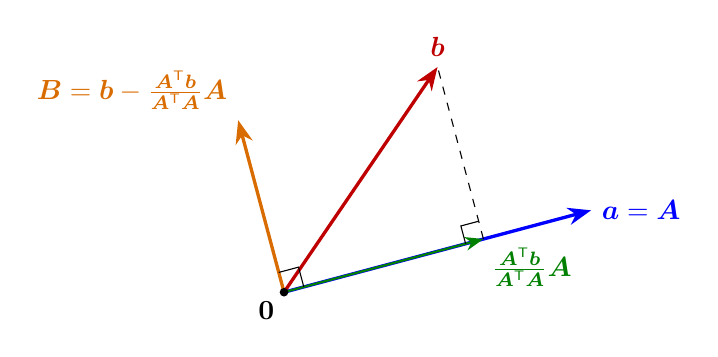
\begin{tikzpicture}[>=Stealth,scale=1.3]
    \draw[->,very thick,blue] (0,0) -- (3,0.8) node[right] {$\vb{a}=\vb{A}$};
    \draw[->,very thick,red!75!black] (0,0) -- (1.5,2.2) node[above] {$\vb{b}$};
    \draw[->,thick,green!50!black] (0,0) -- (1.948,0.5195) node[below right=-1pt] {$\frac{\vb{A}\T\vb{b}}{\vb{A}\T\vb{A}}\vb{A}$};
    \draw[dashed] (1.948,0.5195) -- (1.5,2.2);
    \draw[->,very thick,orange!85!black] (0,0) -- (-0.448,1.6805) node[above left] {$\vb{B}=\vb{b}-\frac{\vb{A}\T\vb{b}}{\vb{A}\T\vb{A}}\vb{A}$};
    \draw[rotate=14.93] (0.2,0) -- (0.2,0.2) -- (0,0.2);
    \draw[shift={(1.948,0.5195)},rotate=14.93] (-0.18,0) -- (-0.18,0.18) -- (0,0.18);
    \fill (0,0) circle (1.2pt) node[below left] {$\vb{0}$};
  \end{tikzpicture}
  \caption{One Gram--Schmidt step. Subtracting from $\vb{b}$ its projection onto $\vb{A}$
  leaves $\vb{B}$, perpendicular to $\vb{A}$ and parallel to the dashed error segment. The
  plane spanned by $\vb{A},\vb{B}$ is the plane spanned by $\vb{a},\vb{b}$.}
  \label{fig:u19-gs}
\end{figure}

\begin{theorem}[Gram--Schmidt]\label{thm:u19-gs}
Let $\vb{a}_1,\dots,\vb{a}_n$ be independent. Define recursively
\[
  \vb{A}_k=\vb{a}_k-\sum_{i<k}(\vb{q}_i\T\vb{a}_k)\,\vb{q}_i,\qquad
  \vb{q}_k=\vb{A}_k/\|\vb{A}_k\|.
\]
Then each $\vb{A}_k\neq\vb{0}$, the vectors $\vb{q}_1,\dots,\vb{q}_n$ are orthonormal, and for
every $k$
\[
  \Span\{\vb{q}_1,\dots,\vb{q}_k\}=\Span\{\vb{a}_1,\dots,\vb{a}_k\}.
\]
\end{theorem}

(Since $\vb{q}_i=\vb{A}_i/\|\vb{A}_i\|$, the term $(\vb{q}_i\T\vb{a}_k)\vb{q}_i$ equals
$\frac{\vb{A}_i\T\vb{a}_k}{\vb{A}_i\T\vb{A}_i}\vb{A}_i$, the form used above.)

\begin{proof}
Induction on $k$. Assume $\vb{q}_1,\dots,\vb{q}_{k-1}$ are orthonormal and span the same
space $V_{k-1}$ as $\vb{a}_1,\dots,\vb{a}_{k-1}$. The vector $\vb{A}_k$ is $\vb{a}_k$ minus an
element of $V_{k-1}$. If $\vb{A}_k$ were $\vb{0}$, then $\vb{a}_k\in V_{k-1}$, contradicting
independence; so $\vb{q}_k$ is defined. For $j<k$,
\[
  \vb{q}_j\T\vb{A}_k=\vb{q}_j\T\vb{a}_k-\sum_{i<k}(\vb{q}_i\T\vb{a}_k)\,\vb{q}_j\T\vb{q}_i
  =\vb{q}_j\T\vb{a}_k-\vb{q}_j\T\vb{a}_k=0,
\]
because only the $i=j$ term survives. So $\vb{q}_k$ is a unit vector orthogonal to the
earlier $\vb{q}$'s. Finally $\vb{q}_k$ is a combination of $\vb{a}_k$ and $V_{k-1}$, and
$\vb{a}_k=\|\vb{A}_k\|\vb{q}_k+\sum_{i<k}(\vb{q}_i\T\vb{a}_k)\vb{q}_i$ is a combination of
$\vb{q}_1,\dots,\vb{q}_k$; hence the two spans agree.
\end{proof}

\begin{example}[Two vectors in \texorpdfstring{$\R^3$}{R3}]\label{ex:u19-lecture}
Let $\vb{a}=(1,1,1)$ and $\vb{b}=(1,0,2)$. Then $\vb{A}=\vb{a}$, $\vb{A}\T\vb{b}=3$,
$\vb{A}\T\vb{A}=3$, and
\[
  \vb{B}=\begin{bmatrix}1\\0\\2\end{bmatrix}-\frac33\begin{bmatrix}1\\1\\1\end{bmatrix}
  =\begin{bmatrix}0\\-1\\1\end{bmatrix},
  \qquad \vb{A}\T\vb{B}=0-1+1=0 .
\]
Dividing by the lengths $\sqrt3$ and $\sqrt2$,
\[
  Q=\begin{bmatrix}\vb{q}_1&\vb{q}_2\end{bmatrix}
  =\begin{bmatrix}1/\sqrt3&0\\1/\sqrt3&-1/\sqrt2\\1/\sqrt3&1/\sqrt2\end{bmatrix}.
\]
The column space of $Q$ is the same plane as the column space of
$\left[\begin{smallmatrix}1&1\\1&0\\1&2\end{smallmatrix}\right]$; only the basis improved.
\end{example}

\begin{trap}
When computing $\vb{C}$, subtract the projections of $\vb{c}$ onto the \emph{new} orthogonal
vectors $\vb{A}$ and $\vb{B}$, not onto the original $\vb{a}$ and $\vb{b}$; the original
vectors are not perpendicular, and subtracting both of their projections over-corrects.
And do not forget the final division by lengths: $\vb{A},\vb{B},\vb{C}$ are orthogonal but
generally not orthonormal. Doing the normalization last keeps square roots out of the
intermediate arithmetic.
\end{trap}

\subsection{\texorpdfstring{$A=QR$}{A = QR}}

Elimination is summarized by $A=LU$; Gram--Schmidt is summarized by a factorization that
connects $A$ to $Q$. Since $\Col{A}=\Col{Q}$, each column of $A$ is a combination of the
$\vb{q}$'s, and the coefficients form a matrix $R$.

\begin{theorem}[\texorpdfstring{$QR$}{QR} factorization]\label{thm:u19-qr}
If $A$ ($m\times n$) has independent columns and $Q$ comes from Gram--Schmidt, then
\[
  A=QR,\qquad R=Q\T A,\qquad r_{ij}=\vb{q}_i\T\vb{a}_j ,
\]
and $R$ is upper triangular with positive diagonal entries $r_{kk}=\|\vb{A}_k\|$.
\end{theorem}

\begin{proof}
Rearranging the definition of $\vb{A}_k$,
$\vb{a}_k=\sum_{i<k}(\vb{q}_i\T\vb{a}_k)\vb{q}_i+\|\vb{A}_k\|\,\vb{q}_k$. This says column $k$
of $A$ equals $Q$ times the column $(r_{1k},\dots,r_{kk},0,\dots,0)$, with
$r_{ik}=\vb{q}_i\T\vb{a}_k$ for $i<k$ and $r_{kk}=\|\vb{A}_k\|>0$; note also
$\vb{q}_k\T\vb{a}_k=\|\vb{A}_k\|$ by dotting the same identity with $\vb{q}_k$. The entries
below the diagonal are zero because $\vb{a}_k$ lies in the span of
$\vb{q}_1,\dots,\vb{q}_k$, so $\vb{q}_i\T\vb{a}_k=0$ for $i>k$: later $\vb{q}$'s are
perpendicular to earlier $\vb{a}$'s. Multiplying $A=QR$ by $Q\T$ gives $R=Q\T A$.
\end{proof}

For two columns,
\[
  \begin{bmatrix}\vb{a}_1&\vb{a}_2\end{bmatrix}
  =\begin{bmatrix}\vb{q}_1&\vb{q}_2\end{bmatrix}
  \begin{bmatrix}\vb{q}_1\T\vb{a}_1&\vb{q}_1\T\vb{a}_2\\0&\vb{q}_2\T\vb{a}_2\end{bmatrix},
\]
and the zero is $\vb{q}_2\T\vb{a}_1=0$ because $\vb{q}_2$ was built perpendicular to
$\vb{a}_1=\vb{A}$. In Example~\ref{ex:u19-lecture}, $\vb{q}_1\T\vb{a}=3/\sqrt3$,
$\vb{q}_1\T\vb{b}=3/\sqrt3$ and $\vb{q}_2\T\vb{b}=2/\sqrt2$, so
\[
  \begin{bmatrix}1&1\\1&0\\1&2\end{bmatrix}
  =\begin{bmatrix}1/\sqrt3&0\\1/\sqrt3&-1/\sqrt2\\1/\sqrt3&1/\sqrt2\end{bmatrix}
   \begin{bmatrix}\sqrt3&\sqrt3\\0&\sqrt2\end{bmatrix}.
\]

\begin{example}[A lucky \texorpdfstring{$3\times 3$}{3 by 3} with no square roots]\label{ex:u19-recitation}
Orthonormalize the columns $\vb{a}=(1,0,0)$, $\vb{b}=(2,0,3)$, $\vb{c}=(4,5,6)$ of
$A=\left[\begin{smallmatrix}1&2&4\\0&0&5\\0&3&6\end{smallmatrix}\right]$, working directly
with unit vectors.
\begin{itemize}
  \item $\vb{a}$ already has length $1$: $\vb{q}_1=(1,0,0)$.
  \item $\vb{b}-(\vb{b}\T\vb{q}_1)\vb{q}_1=(2,0,3)-2(1,0,0)=(0,0,3)$, of length $3$, so
    $\vb{q}_2=(0,0,1)$.
  \item $\vb{c}-(\vb{c}\T\vb{q}_1)\vb{q}_1-(\vb{c}\T\vb{q}_2)\vb{q}_2=(4,5,6)-4(1,0,0)-6(0,0,1)=(0,5,0)$,
    of length $5$, so $\vb{q}_3=(0,1,0)$.
\end{itemize}
The numbers subtracted and the lengths are exactly the entries of $R$:
\[
  \underbrace{\begin{bmatrix}1&2&4\\0&0&5\\0&3&6\end{bmatrix}}_{A}
  =\underbrace{\begin{bmatrix}1&0&0\\0&0&1\\0&1&0\end{bmatrix}}_{Q}
   \underbrace{\begin{bmatrix}1&2&4\\0&3&6\\0&0&5\end{bmatrix}}_{R},
\]
which reads column by column as $\vb{a}=1\vb{q}_1$, $\vb{b}=2\vb{q}_1+3\vb{q}_2$,
$\vb{c}=4\vb{q}_1+6\vb{q}_2+5\vb{q}_3$. Here $Q$ happens to be a permutation matrix, and $R$
is $A$ with rows~2 and~3 exchanged.
\end{example}

\paragraph{Least squares with \texorpdfstring{$A=QR$}{A = QR}.}
Substituting $A=QR$ into the normal equations,
$R\T Q\T QR\hat{\vb{x}}=R\T Q\T\vb{b}$ becomes $R\T R\hat{\vb{x}}=R\T Q\T\vb{b}$, and since $R$
is invertible,
\[
  R\hat{\vb{x}}=Q\T\vb{b},
\]
a triangular system solved by back substitution. This is how least squares is computed in
practice.

\begin{example}[The best-fit line again, via \texorpdfstring{$QR$}{QR}]\label{ex:u19-short}
For the data $(0,6),(1,0),(2,0)$ of Section~\ref{sec:u18}, $A$ has columns
$\vb{a}_1=(1,1,1)$ and $\vb{a}_2=(0,1,2)$, and $\vb{b}=(6,0,0)$. Gram--Schmidt:
$\vb{A}_2=(0,1,2)-\frac33(1,1,1)=(-1,0,1)$, so
\[
  \vb{q}_1=\tfrac{1}{\sqrt3}(1,1,1),\quad \vb{q}_2=\tfrac{1}{\sqrt2}(-1,0,1),\qquad
  R=\begin{bmatrix}\sqrt3&\sqrt3\\0&\sqrt2\end{bmatrix},\qquad
  Q\T\vb{b}=\begin{bmatrix}6/\sqrt3\\-6/\sqrt2\end{bmatrix}=\begin{bmatrix}2\sqrt3\\-3\sqrt2\end{bmatrix}.
\]
Back substitution in $R\hat{\vb{x}}=Q\T\vb{b}$: $\sqrt2\,D=-3\sqrt2$ gives $D=-3$, then
$\sqrt3\,C+\sqrt3\,D=2\sqrt3$ gives $C=5$, the same line $b=5-3t$. The projection is a sum of
two independent one-dimensional projections:
$\vb{p}=\vb{q}_1(\vb{q}_1\T\vb{b})+\vb{q}_2(\vb{q}_2\T\vb{b})=2(1,1,1)-3(-1,0,1)=(5,2,-1)$.
\end{example}

\subsection{Exercises}

\begin{exercise}\label{ex:u19-indep}
Orthonormal vectors are automatically independent. Give a matrix proof: if $Q$ has
orthonormal columns, show that $Q\vb{x}=\vb{0}$ implies $\vb{x}=\vb{0}$. ($Q$ may be
rectangular, so use $Q\T$, not $Q^{-1}$.)
\end{exercise}

\begin{solution}
Multiply $Q\vb{x}=\vb{0}$ by $Q\T$: $Q\T Q\vb{x}=Q\T\vb{0}$, i.e.\ $I\vb{x}=\vb{0}$, so
$\vb{x}=\vb{0}$. Thus $\Nul{Q}=\{\vb{0}\}$ and no nontrivial combination of the columns
vanishes.
\end{solution}

\begin{exercise}\label{ex:u19-perpd}
Apply Gram--Schmidt to $\vb{a}=(1,-1,0,0)$, $\vb{b}=(0,1,-1,0)$, $\vb{c}=(0,0,1,-1)$ to get
orthogonal vectors $\vb{A},\vb{B},\vb{C}$. Show that $\{\vb{A},\vb{B},\vb{C}\}$ and
$\{\vb{a},\vb{b},\vb{c}\}$ are both bases for the space of vectors perpendicular to
$\vb{d}=(1,1,1,1)$.
\end{exercise}

\begin{solution}
$\vb{A}=\vb{a}=(1,-1,0,0)$. Then $\vb{A}\T\vb{b}=-1$, $\vb{A}\T\vb{A}=2$, and
$\vb{B}=\vb{b}+\frac12\vb{A}=(\frac12,\frac12,-1,0)$. Next $\vb{A}\T\vb{c}=0$,
$\vb{B}\T\vb{c}=-1$, $\vb{B}\T\vb{B}=\frac32$, so
$\vb{C}=\vb{c}+\frac23\vb{B}=(\frac13,\frac13,\frac13,-1)$. The three are mutually orthogonal
(check the three dot products) and each has components summing to zero, so each is
perpendicular to $\vb{d}$; so are $\vb{a},\vb{b},\vb{c}$. The space $\vb{d}^{\perp}$ is the
nullspace of the $1\times 4$ matrix $\vb{d}\T$, of dimension $4-1=3$. Three independent
vectors in a $3$-dimensional space form a basis. $\vb{A},\vb{B},\vb{C}$ are independent
because they are orthogonal and nonzero (normalize them and use Exercise~\ref{ex:u19-indep}).
For $\vb{a},\vb{b},\vb{c}$: the combination
$x_1\vb{a}+x_2\vb{b}+x_3\vb{c}=(x_1,\,x_2-x_1,\,x_3-x_2,\,-x_3)$ is zero only when
$x_1=x_2=x_3=0$.
\end{solution}

\begin{exercise}\label{ex:u19-qr}
Find the $QR$ factorization of $A=\begin{bmatrix}1&1\\2&0\\2&1\end{bmatrix}$.
\end{exercise}

\begin{solution}
$\|\vb{a}_1\|=3$, so $\vb{q}_1=\frac13(1,2,2)$ and $r_{11}=3$. Next
$r_{12}=\vb{q}_1\T\vb{a}_2=\frac{1+0+2}{3}=1$, and
$\vb{A}_2=\vb{a}_2-\vb{q}_1=(1,0,1)-\frac13(1,2,2)=\frac13(2,-2,1)$, which already has length
$1$; so $\vb{q}_2=\frac13(2,-2,1)$ and $r_{22}=1$. Hence
\[
  A=\frac13\begin{bmatrix}1&2\\2&-2\\2&1\end{bmatrix}\begin{bmatrix}3&1\\0&1\end{bmatrix},
\]
and multiplying out reproduces the columns $(1,2,2)$ and $(1,0,1)$.
\end{solution}

\begin{exercise}\label{ex:u19-length}
Show that multiplication by a matrix with orthonormal columns preserves lengths and dot
products: $\|Q\vb{x}\|=\|\vb{x}\|$ and $(Q\vb{x})\T(Q\vb{y})=\vb{x}\T\vb{y}$. What does this
say about the rotation matrices of Example~\ref{ex:u19-gallery}?
\end{exercise}

\begin{solution}
$(Q\vb{x})\T(Q\vb{y})=\vb{x}\T Q\T Q\vb{y}=\vb{x}\T\vb{y}$; taking $\vb{y}=\vb{x}$ gives
$\|Q\vb{x}\|^2=\|\vb{x}\|^2$. Rotations therefore move vectors without stretching them and
preserve the angles between them, as a rigid rotation of the plane should.
\end{solution}

% unit: u20
% sources: sources/079-properties-of-determinants.txt, sources/035-lecture-18-properties-of-determinants.txt, sources/185-mit18-06scf11-ses2-5sum-pdf-download-file.txt, sources/036-problem-solving-properties-of-determinants.txt, sources/186-mit18-06scf11-ses2-5prob-pdf-download-file.txt, sources/187-mit18-06scf11-ses2-5sol-pdf-download-file.txt
\section{Properties of determinants}\label{sec:u20}

Up to now most of our matrices were rectangular. The second half of the course concentrates on
\emph{square} matrices, and its two big tools are the determinant and the eigenvalues; the
determinant comes first because eigenvalues will be found from it. The determinant of a
square matrix $A$, written $\det A$ or $|A|$, is a single number that packs in a remarkable
amount of information, above all: $A$ is invertible exactly when $\det A\neq 0$. Rather than
start from a formula (that comes in Section~\ref{sec:u21}), we start from three properties.
Everything else, including the familiar $ad-bc$ and an efficient way to compute, follows from
them.

\subsection{Three properties define the determinant}

\begin{definition}[The determinant]\label{def:u20-det}
The determinant is the function assigning a number $\det A$ to each $n\times n$ matrix such
that:
\begin{enumerate}[1.]
  \item $\det I=1$.
  \item Exchanging two rows reverses the sign of the determinant.
  \item The determinant is linear in each row separately (the other rows held fixed):
    \begin{enumerate}[(a)]
      \item multiplying one row by $t$ multiplies the determinant by $t$;
      \item if one row is a sum $\vb{r}+\vb{r}'$, the determinant is the sum of the two
        determinants with that row replaced by $\vb{r}$ and by $\vb{r}'$.
    \end{enumerate}
\end{enumerate}
\end{definition}

For $2\times 2$ matrices, with vertical bars denoting determinants:
\[
  \text{(3a)}\ \ \begin{vmatrix}ta&tb\\c&d\end{vmatrix}=t\begin{vmatrix}a&b\\c&d\end{vmatrix},
  \qquad
  \text{(3b)}\ \ \begin{vmatrix}a+a'&b+b'\\c&d\end{vmatrix}
  =\begin{vmatrix}a&b\\c&d\end{vmatrix}+\begin{vmatrix}a'&b'\\c&d\end{vmatrix}.
\]
Properties 1 and 2 already give every permutation matrix: $\det P=+1$ if $P$ comes from $I$
by an even number of row exchanges and $-1$ if by an odd number. For instance
$\left|\begin{smallmatrix}1&0\\0&1\end{smallmatrix}\right|=1$ and
$\left|\begin{smallmatrix}0&1\\1&0\end{smallmatrix}\right|=-1$. Hidden here is a fact that we
take on trust until Section~\ref{sec:u21}: a permutation can never be reached both by an even
and by an odd number of exchanges. Without it, property 2 could force $\det P=-\det P$, and
the three properties would contradict each other.

\begin{trap}
Property 3 is linearity in \emph{one row at a time}. It does \emph{not} say
$\det(A+B)=\det A+\det B$, which is false: for
$A=\left[\begin{smallmatrix}1&2\\3&4\end{smallmatrix}\right]$ and
$B=\left[\begin{smallmatrix}2&0\\1&1\end{smallmatrix}\right]$, $\det A=-2$ and $\det B=2$,
but $\det(A+B)=\left|\begin{smallmatrix}3&2\\4&5\end{smallmatrix}\right|=7$. Nor does it say
$\det(2A)=2\det A$: the factor $2$ comes out of \emph{every} row, so
$\det(2A)=2^n\det A$ for an $n\times n$ matrix, just as doubling the sides of a box in
$\R^3$ multiplies its volume by $2^3=8$.
\end{trap}

\subsection{Seven consequences}

Each of the following is derived from properties 1--3 alone. The proofs are short, and they
are the reason the properties are worth learning: they explain why elimination computes
determinants.

\begin{proposition}[Property 4: equal rows]\label{prop:u20-equal}
If two rows of $A$ are equal, then $\det A=0$.
\end{proposition}

\begin{proof}
Exchanging the two equal rows leaves $A$ unchanged, so the determinant is unchanged; by
property 2 it also changes sign. So $\det A=-\det A$, and $\det A=0$.
\end{proof}

\begin{proposition}[Property 5: elimination does not change the determinant]\label{prop:u20-elim}
Subtracting $\ell$ times row $i$ from row $k$ ($i\neq k$) leaves $\det A$ unchanged.
\end{proposition}

\begin{proof}
By linearity in row $k$ (3b, then 3a), the new determinant is $\det A$ minus $\ell$ times the
determinant of the matrix whose row $k$ is a copy of row $i$. That matrix has two equal rows,
so its determinant is $0$ by property 4. In the $2\times 2$ case:
\[
  \begin{vmatrix}a&b\\c-\ell a&d-\ell b\end{vmatrix}
  =\begin{vmatrix}a&b\\c&d\end{vmatrix}-\ell\begin{vmatrix}a&b\\a&b\end{vmatrix}
  =\begin{vmatrix}a&b\\c&d\end{vmatrix}.\qedhere
\]
\end{proof}

\begin{proposition}[Property 6: zero row]\label{prop:u20-zero}
If $A$ has a row of zeros, then $\det A=0$.
\end{proposition}

\begin{proof}
Multiply the zero row by $t=0$: the matrix does not change, and by 3a the determinant is
multiplied by $0$.
\end{proof}

\begin{proposition}[Property 7: triangular matrices]\label{prop:u20-triangular}
If $U$ is triangular with diagonal entries $d_1,\dots,d_n$, then $\det U=d_1d_2\cdots d_n$.
\end{proposition}

\begin{proof}
Suppose $U$ is upper triangular (the lower case is the same). If all $d_i\neq 0$, use each
diagonal entry, from the bottom up, to eliminate the entries above it; by property 5 this does
not change the determinant and it leaves the diagonal matrix $D=\operatorname{diag}(d_1,\dots,d_n)$.
Factor $d_i$ out of row $i$ for each $i$ (property 3a) to get $d_1\cdots d_n\det I$, and
$\det I=1$. If some $d_i=0$, elimination produces a full row of zeros instead (take the
lowest zero on the diagonal: the rows below it can clear everything in its row), and property 6
gives $\det U=0=d_1\cdots d_n$.
\end{proof}

\begin{theorem}[Property 8: the invertibility test]\label{thm:u20-singular}
$\det A=0$ exactly when $A$ is singular. If elimination with $k$ row exchanges reduces $A$
to $U$ with pivots $d_1,\dots,d_n$, then
\[
  \det A=(-1)^k\,d_1d_2\cdots d_n .
\]
\end{theorem}

\begin{proof}
Elimination uses only subtractions of multiples of rows (no change, property 5) and row
exchanges (a sign change each, property 2), so $\det A=(-1)^k\det U$. If $A$ is singular,
elimination produces a zero row and $\det U=0$ (property 6). If $A$ is invertible, there are
$n$ nonzero pivots and $\det U=d_1\cdots d_n\neq 0$ (property 7).
\end{proof}

This ``product of the pivots'' is how software computes determinants: an $n\times n$
elimination costs about $n^3/3$ operations, while the formulas of Section~\ref{sec:u21} have
$n!$ terms. The proof also shows that properties 1--3 leave no freedom: any function
satisfying them must equal $(-1)^k d_1\cdots d_n$ on every matrix. We use this uniqueness
below.

\begin{example}[\texorpdfstring{$ad-bc$}{ad - bc} from the pivots]\label{ex:u20-2by2}
If $a\neq 0$, subtract $c/a$ times row~1 from row~2:
\[
  \begin{vmatrix}a&b\\c&d\end{vmatrix}=\begin{vmatrix}a&b\\0&d-\frac{c}{a}b\end{vmatrix}
  =a\Bigl(d-\frac{cb}{a}\Bigr)=ad-bc .
\]
If $a=0$, exchange the rows first:
$\left|\begin{smallmatrix}0&b\\c&d\end{smallmatrix}\right|=-\left|\begin{smallmatrix}c&d\\0&b\end{smallmatrix}\right|=-cb$,
again $ad-bc$. (If also $c=0$, the first column is zero, $A$ is singular, and both sides are
$0$.) For instance $\left|\begin{smallmatrix}0&2\\3&4\end{smallmatrix}\right|=-(3\cdot 2)=-6$.
\end{example}

\begin{example}[A \texorpdfstring{$3\times 3$}{3 by 3} determinant by elimination]\label{ex:u20-3by3}
\[
  A=\begin{bmatrix}2&1&1\\4&-6&0\\-2&7&2\end{bmatrix}
  \longrightarrow
  \begin{bmatrix}2&1&1\\0&-8&-2\\0&8&3\end{bmatrix}
  \longrightarrow
  \begin{bmatrix}2&1&1\\0&-8&-2\\0&0&1\end{bmatrix}=U .
\]
The steps subtract $2$ (row~1) from row~2, add row~1 to row~3, then add row~2 to row~3; none
changes the determinant and there were no exchanges. So
$\det A=2\cdot(-8)\cdot 1=-16$.
\end{example}

Figure~\ref{fig:u20-shear} shows what property 5 means geometrically for $2\times 2$
matrices, where $|\det A|$ is the area of the parallelogram spanned by the rows (proved in
Section~\ref{sec:u22}).

\begin{figure}[ht]
  \centering
  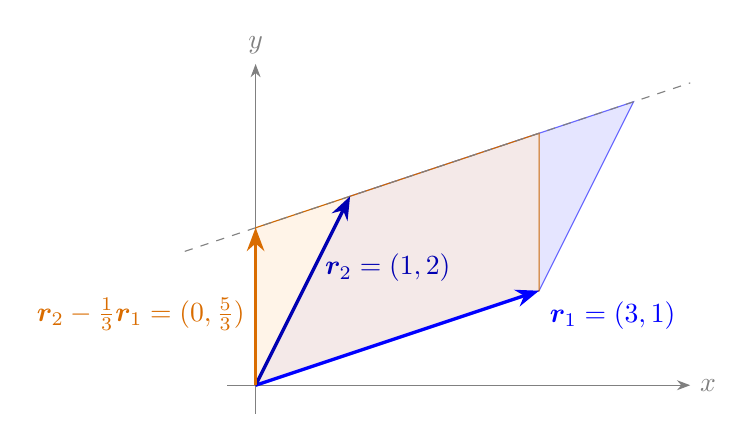
\begin{tikzpicture}[>=Stealth,scale=1.2]
    \draw[->,gray] (-0.3,0) -- (4.6,0) node[right] {$x$};
    \draw[->,gray] (0,-0.3) -- (0,3.4) node[above] {$y$};
    \filldraw[fill=blue!10,draw=blue!60] (0,0) -- (3,1) -- (4,3) -- (1,2) -- cycle;
    \filldraw[fill=orange!15,draw=orange!80!black,fill opacity=0.6] (0,0) -- (3,1) -- (3,8/3) -- (0,5/3) -- cycle;
    \draw[dashed,gray] (-0.75,1.4167) -- (4.6,3.2);
    \draw[->,very thick,blue] (0,0) -- (3,1) node[below right] {$\vb{r}_1=(3,1)$};
    \draw[->,very thick,blue!70!black] (0,0) -- (1,2) node[pos=0.62,right] {$\vb{r}_2=(1,2)$};
    \draw[->,very thick,orange!85!black] (0,0) -- (0,5/3) node[pos=0.45,left] {$\vb{r}_2-\frac13\vb{r}_1=(0,\frac53)$};
  \end{tikzpicture}
  \caption{Subtracting a multiple of row~1 from row~2 slides $\vb{r}_2$ along the dashed line
  parallel to $\vb{r}_1$. Base and height are unchanged, so the area stays
  $\left|\begin{smallmatrix}3&1\\1&2\end{smallmatrix}\right|=6-1=5$; the new matrix
  $\left[\begin{smallmatrix}3&1\\0&5/3\end{smallmatrix}\right]$ is triangular, and its pivots
  give $3\cdot\frac53=5$.}
  \label{fig:u20-shear}
\end{figure}

\begin{theorem}[Property 9: the product rule]\label{thm:u20-product}
For $n\times n$ matrices, $\det(AB)=(\det A)(\det B)$. In particular
$\det A^{-1}=1/\det A$ when $A$ is invertible, and $\det A^2=(\det A)^2$.
\end{theorem}

\begin{proof}
If $\det B=0$, then $B$ is singular: some $\vb{x}\neq\vb{0}$ has $B\vb{x}=\vb{0}$, so
$AB\vb{x}=\vb{0}$, $AB$ is singular, and both sides are $0$. If $\det B\neq 0$, consider the
function $D(A)=\det(AB)/\det B$ of the matrix $A$. It satisfies the three defining
properties: $D(I)=1$; exchanging two rows of $A$ exchanges the same two rows of $AB$, so $D$
changes sign; and row $i$ of $AB$ is (row $i$ of $A$) times $B$, which depends linearly on row
$i$ of $A$, so $D$ is linear in each row. By uniqueness (the remark after
Theorem~\ref{thm:u20-singular}), $D(A)=\det A$, which is the product rule. Applying it to
$A^{-1}A=I$ gives $\det A^{-1}\det A=1$.
\end{proof}

For diagonal matrices the rule is plain: $A=\operatorname{diag}(2,3)$ has $\det A=6$ and
$A^{-1}=\operatorname{diag}(\frac12,\frac13)$ has determinant $\frac16$.

\begin{theorem}[Property 10: transpose]\label{thm:u20-transpose}
$\det A\T=\det A$.
\end{theorem}

\begin{proof}
If $A$ is singular, so is $A\T$ (same rank), and both determinants are $0$. Otherwise
elimination gives $PA=LU$ with $P$ a permutation, $L$ lower triangular with ones on the
diagonal and $U$ upper triangular. Since $P\T P=I$, $A=P\T LU$ and $A\T=U\T L\T P$. By the
product rule and property 7,
\[
  \det A=\det P\T\cdot 1\cdot\det U,\qquad \det A\T=\det U\T\cdot 1\cdot\det P ,
\]
with $\det U\T=\det U$ (same diagonal). Finally $\det P\T\det P=\det(P\T P)=1$ and
$\det P=\pm1$, so $\det P\T=\det P$.
\end{proof}

Property 10 turns every statement about rows into one about columns: a zero column gives
$\det A=0$, exchanging two columns reverses the sign, and the determinant is linear in each
column separately.

\begin{example}[Four quick determinants]\label{ex:u20-recitation}
Each of these needs only one or two of the properties.
\begin{enumerate}[(a)]
  \item Subtracting row~1 from row~2 and row~2 from row~3 (property 5) produces two rows
    equal to $(1,1,1)$, so by property 4
    \[
      \begin{vmatrix}101&201&301\\102&202&302\\103&203&303\end{vmatrix}
      =\begin{vmatrix}101&201&301\\1&1&1\\1&1&1\end{vmatrix}=0 .
    \]
  \item The rank-one matrix
    $C=\begin{bmatrix}1\\2\\3\end{bmatrix}\begin{bmatrix}1&-4&5\end{bmatrix}$ has rows that
    are $1,2,3$ times the same row, so $C$ is singular and $\det C=0$ (property 8).
  \item The skew-symmetric matrix
    $D=\left[\begin{smallmatrix}0&1&3\\-1&0&4\\-3&-4&0\end{smallmatrix}\right]$ has
    $D\T=-D$. Then $\det D=\det D\T=\det(-D)=(-1)^3\det D$, so $\det D=0$.
  \item $\det\left[\begin{smallmatrix}0&1\\-1&0\end{smallmatrix}\right]=1$: for even $n$ the
    argument in (c) gives only $\det D=\det D$, and skew-symmetric matrices can be invertible.
\end{enumerate}
\end{example}

\subsection{Exercises}

\begin{exercise}\label{ex:u20-rowsums}
If the entries in every row of a square matrix $A$ add to zero, solve $A\vb{x}=\vb{0}$ to
prove $\det A=0$. If those entries add to one, show that $\det(A-I)=0$. Does this mean
$\det A=1$?
\end{exercise}

\begin{solution}
If every row sums to zero, then $\vb{x}=(1,1,\dots,1)$ satisfies $A\vb{x}=\vb{0}$, because each
component of $A\vb{x}$ is a row sum. A nonzero nullspace means $A$ is singular, so
$\det A=0$. If every row sums to one, every row of $A-I$ sums to zero, so $\det(A-I)=0$. This
does not force $\det A=1$: the rows of $A=\left[\begin{smallmatrix}0&1\\1&0\end{smallmatrix}\right]$
sum to one, but $\det A=-1$.
\end{solution}

\begin{exercise}[Vandermonde determinant]\label{ex:u20-vandermonde}
Use row operations and the properties to show
\[
  \det\begin{bmatrix}1&a&a^2\\1&b&b^2\\1&c&c^2\end{bmatrix}=(b-a)(c-a)(c-b).
\]
\end{exercise}

\begin{solution}
Subtract row~1 from rows~2 and~3 (no change), then factor $b-a$ out of row~2 and $c-a$ out of
row~3 (property 3a), using $b^2-a^2=(b-a)(b+a)$:
\[
  \begin{vmatrix}1&a&a^2\\0&b-a&b^2-a^2\\0&c-a&c^2-a^2\end{vmatrix}
  =(b-a)(c-a)\begin{vmatrix}1&a&a^2\\0&1&b+a\\0&1&c+a\end{vmatrix}
  =(b-a)(c-a)\begin{vmatrix}1&a&a^2\\0&1&b+a\\0&0&c-b\end{vmatrix},
\]
where the last step subtracts row~2 from row~3. The matrix is now triangular with diagonal
$1,1,c-b$, so the determinant is $(b-a)(c-a)(c-b)$. It is zero exactly when two of $a,b,c$
coincide, i.e.\ when two rows are equal.
\end{solution}

\begin{exercise}\label{ex:u20-scaling}
A $3\times 3$ matrix $A$ has $\det A=5$. Find $\det(2A)$, $\det(-A)$, $\det(A^2)$,
$\det(A^{-1})$ and $\det(A\T)$.
\end{exercise}

\begin{solution}
$\det(2A)=2^3\cdot 5=40$; $\det(-A)=(-1)^3\cdot 5=-5$; $\det(A^2)=5^2=25$;
$\det(A^{-1})=\frac15$; $\det(A\T)=5$.
\end{solution}

\begin{exercise}\label{ex:u20-skew}
Show that every skew-symmetric matrix ($D\T=-D$) of odd size $n$ has $\det D=0$.
\end{exercise}

\begin{solution}
$\det D=\det D\T=\det(-D)=(-1)^n\det D=-\det D$ for odd $n$, using property 10 and
property 3a applied to each of the $n$ rows. Hence $\det D=0$. Example~\ref{ex:u20-recitation}(d)
shows that the conclusion fails for even $n$.
\end{solution}

% unit: u21
% sources: sources/083-determinant-formulas-and-cofactors.txt, sources/037-lecture-19-determinant-formulas-and-cofactors.txt, sources/188-mit18-06scf11-ses2-6sum-pdf-download-file.txt, sources/038-problem-solving-determinants.txt, sources/189-mit18-06scf11-ses2-6prob-pdf-download-file.txt, sources/190-mit18-06scf11-ses2-6sol-pdf-download-file.txt
\section{Determinant formulas and cofactors}\label{sec:u21}

Section~\ref{sec:u20} defined the determinant by three properties and computed it by
elimination: $\det A$ is $\pm$ the product of the pivots. This section derives two explicit
formulas from the same properties. The \emph{big formula} writes $\det A$ as a sum of $n!$
signed products, one entry from each row and each column. The \emph{cofactor formula} groups
those products to express an $n\times n$ determinant through determinants of size $n-1$. We
finish with a family of tridiagonal matrices whose determinants repeat with period six.

\subsection{Splitting the rows: from \texorpdfstring{$2\times 2$}{2 by 2} to the big formula}

Linearity in each row (property 3) lets us split a row into pieces. For a $2\times 2$ matrix
split row~1 as $(a,b)=(a,0)+(0,b)$, then split row~2 in each piece:
\[
  \begin{vmatrix}a&b\\c&d\end{vmatrix}
  =\begin{vmatrix}a&0\\c&d\end{vmatrix}+\begin{vmatrix}0&b\\c&d\end{vmatrix}
  =\begin{vmatrix}a&0\\c&0\end{vmatrix}+\begin{vmatrix}a&0\\0&d\end{vmatrix}
  +\begin{vmatrix}0&b\\c&0\end{vmatrix}+\begin{vmatrix}0&b\\0&d\end{vmatrix}.
\]
The first and last pieces have a zero column, so they are singular and vanish. The second is
diagonal, $ad$. The third is $bc$ times the determinant of the row exchange
$\left[\begin{smallmatrix}0&1\\1&0\end{smallmatrix}\right]$, which is $-1$. So
$\det A=ad-bc$, now derived rather than remembered.

For a $3\times 3$ matrix the same splitting produces $3\cdot 3\cdot 3=27$ pieces, each with
one entry from each row. A piece survives only if its three entries also lie in three
\emph{different columns}; otherwise it has a zero column. The survivors are the six patterns of
Figure~\ref{fig:u21-survivors}, and each equals the product of its entries times the
determinant of a permutation matrix:
\[
  \det A=a_{11}a_{22}a_{33}-a_{11}a_{23}a_{32}-a_{12}a_{21}a_{33}+a_{12}a_{23}a_{31}
  +a_{13}a_{21}a_{32}-a_{13}a_{22}a_{31}.
\]
For example the term $a_{12}a_{23}a_{31}$ uses columns $(2,3,1)$; two exchanges (rows 1 and
3, then rows 2 and 3) restore the order $(1,2,3)$, so its sign is $+$.

\begin{figure}[ht]
  \centering
  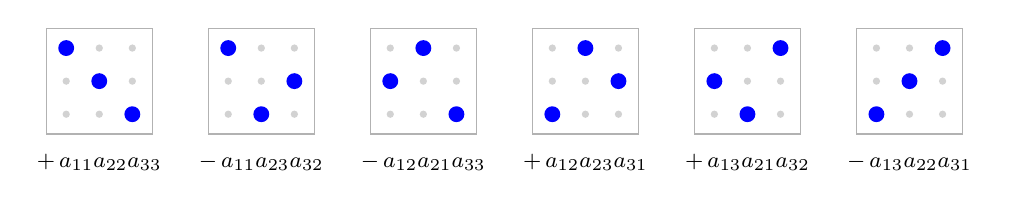
\begin{tikzpicture}[scale=0.42,font=\footnotesize]
    \foreach \a/\b/\c/\sg [count=\k from 0] in {1/2/3/+, 1/3/2/-, 2/1/3/-, 2/3/1/+, 3/1/2/+, 3/2/1/-}{
      \begin{scope}[shift={(\k*4.9,0)}]
        \draw[gray!60] (0.4,0.4) rectangle (3.6,3.6);
        \foreach \i in {1,2,3} {\foreach \j in {1,2,3} {\fill[gray!35] (\j,4-\i) circle (0.11);}}
        \fill[blue] (\a,3) circle (0.24);
        \fill[blue] (\b,2) circle (0.24);
        \fill[blue] (\c,1) circle (0.24);
        \node at (2,-0.45) {$\sg\,a_{1\a}a_{2\b}a_{3\c}$};
      \end{scope}}
  \end{tikzpicture}
  \caption{The six nonzero pieces of a $3\times 3$ determinant: one entry from each row and
  each column, i.e.\ the positions of the $1$'s in a permutation matrix. The sign is the
  determinant of that permutation matrix: $+$ for an even number of row exchanges, $-$ for an
  odd number.}
  \label{fig:u21-survivors}
\end{figure}

\begin{definition}[Sign of a permutation]\label{def:u21-sign}
A permutation $\sigma$ of $\{1,\dots,n\}$ corresponds to the permutation matrix $P_\sigma$
whose row $i$ has its $1$ in column $\sigma(i)$. Its \emph{sign} is
$\operatorname{sgn}\sigma=\det P_\sigma$, which is $+1$ if $P_\sigma$ is reached from $I$ by
an even number of row exchanges and $-1$ if by an odd number.
\end{definition}

\begin{theorem}[The big formula]\label{thm:u21-big}
For an $n\times n$ matrix $A$,
\[
  \det A=\sum_{\sigma}\operatorname{sgn}(\sigma)\,a_{1\sigma(1)}a_{2\sigma(2)}\cdots a_{n\sigma(n)},
\]
the sum running over all $n!$ permutations $\sigma=(\alpha,\beta,\dots,\omega)$ of the column
numbers.
\end{theorem}

\begin{proof}
Write row $i$ of $A$ as $\sum_j a_{ij}\vb{e}_j\T$, where $\vb{e}_j\T$ is row $j$ of $I$. Using
linearity in row~1, then in row~2, and so on, $\det A$ becomes a sum over all choices of
column numbers $(j_1,\dots,j_n)$:
\[
  \det A=\sum_{j_1,\dots,j_n}a_{1j_1}a_{2j_2}\cdots a_{nj_n}\,
  \det\begin{bmatrix}\vb{e}_{j_1}\T\\ \vdots\\ \vb{e}_{j_n}\T\end{bmatrix}.
\]
If two of the $j$'s coincide, the last matrix has two equal rows and its determinant is $0$.
Otherwise $(j_1,\dots,j_n)$ is a permutation $\sigma$ and the matrix is $P_\sigma$, whose
determinant is $\operatorname{sgn}\sigma$.
\end{proof}

Why $n!$ terms: the entry from row~1 can be chosen in $n$ columns, the entry from row~2 in the
$n-1$ columns still unused, and so on: $2$ terms for $n=2$, $6$ for $n=3$, $24$ for $n=4$.
Half have each sign (for $n\ge 2$). The formula reproduces the properties; for instance
$\det I=1$ because only the identity permutation picks no zero entry of $I$. Conversely, the
formula \emph{defines} a function with properties 1--3, which settles the loose end of
Section~\ref{sec:u20}: the determinant exists, so a permutation cannot be both even and odd.

\begin{trap}
The ``down-right diagonals are $+$, down-left diagonals are $-$'' picture of the $3\times 3$
formula does not extend to $4\times 4$. The $4\times 4$ anti-diagonal permutation $(4,3,2,1)$
needs two exchanges (rows 1 and 4, rows 2 and 3), so its term carries a $+$ sign. Always count
exchanges, or use cofactors.
\end{trap}

\begin{example}[Most terms vanish]\label{ex:u21-sparse}
For
\[
  A=\begin{bmatrix}0&0&1&1\\0&1&1&0\\1&1&0&0\\1&0&0&1\end{bmatrix}
\]
look for ways to pick a nonzero entry in every row and column. Row~1 can use column~3 or
column~4, and each choice forces the rest. If row~1 uses column~4, row~4 must use column~1,
then row~3 column~2 and row~2 column~3: the permutation $(4,3,2,1)$, sign $+$, contributing
$+1$. If row~1 uses column~3, row~2 must use column~2, row~3 column~1 and row~4 column~4:
the permutation $(3,2,1,4)$, which one exchange (rows 1 and 3 of its permutation matrix) puts
in order, so its sign is $-$ and it contributes $-1$.
Row~1 has no other nonzero entries, so these are the only two of the $24$ terms, and
$\det A=1-1=0$. The matrix must be singular, and indeed
row~1 $-$ row~2 $+$ row~3 $-$ row~4 $=\vb{0}$.
\end{example}

\subsection{Cofactors}

Collect the terms of the big formula that contain a particular entry $a_{1j}$. What
multiplies $a_{1j}$ is built from the other rows and the other columns, one entry from each:
it is (up to sign) a determinant of size $n-1$.

\begin{definition}[Minor and cofactor]\label{def:u21-cofactor}
The \emph{minor} $M_{ij}$ is the $(n-1)\times(n-1)$ matrix obtained from $A$ by deleting row
$i$ and column $j$. The \emph{cofactor} of $a_{ij}$ is
\[
  C_{ij}=(-1)^{i+j}\det M_{ij}.
\]
The signs $(-1)^{i+j}$ form a checkerboard starting with $+$ in the top-left corner.
\end{definition}

\begin{theorem}[Cofactor expansion]\label{thm:u21-cofactor}
For each row $i$,
\[
  \det A=a_{i1}C_{i1}+a_{i2}C_{i2}+\cdots+a_{in}C_{in},
\]
and likewise down each column $j$: $\det A=a_{1j}C_{1j}+\cdots+a_{nj}C_{nj}$.
\end{theorem}

\begin{proof}
\emph{Row 1.} By linearity in row~1, $\det A=\sum_j a_{1j}\det A_j$, where $A_j$ is $A$ with
row~1 replaced by $\vb{e}_j\T$. In $A_j$ subtract multiples of row~1 from the other rows to
clear column $j$ below the $1$ (property 5, no change). Then move column $j$ to the front by
$j-1$ exchanges of neighbouring columns; each reverses the sign (exchanging columns is allowed
because $\det A\T=\det A$), and the other columns keep their order. The result is the block matrix
\[
  \begin{bmatrix}1&\vb{0}\T\\ \vb{0}&M_{1j}\end{bmatrix}.
\]
Its determinant is $\det M_{1j}$, because as a function of the $(n-1)\times(n-1)$ matrix $M$,
the determinant of $\left[\begin{smallmatrix}1&\vb{0}\T\\ \vb{0}&M\end{smallmatrix}\right]$
satisfies the three defining properties, so it equals $\det M$ by uniqueness
(Section~\ref{sec:u20}). Hence $\det A_j=(-1)^{j-1}\det M_{1j}=C_{1j}$.

\emph{Row $i$.} Move row $i$ to the top by $i-1$ exchanges of neighbouring rows, keeping the
other rows in order. The determinant gains the factor $(-1)^{i-1}$, the new first row is row
$i$ of $A$, and its minors are the $M_{ij}$. So
$\det A=(-1)^{i-1}\sum_j a_{ij}(-1)^{1+j}\det M_{ij}=\sum_j a_{ij}C_{ij}$.

\emph{Columns.} Apply the row expansion to $A\T$.
\end{proof}

For a $2\times 2$ matrix the cofactors along row~1 are $C_{11}=d$ and $C_{12}=-c$, giving
$ad+b(-c)$. For $3\times 3$ the expansion along row~1 is
\[
  \det A=a_{11}(a_{22}a_{33}-a_{23}a_{32})+a_{12}(-a_{21}a_{33}+a_{23}a_{31})+a_{13}(a_{21}a_{32}-a_{22}a_{31}),
\]
which is the six-term formula regrouped; the middle parenthesis carries the minus sign of the
$(1,2)$ position.

\begin{example}[Expanding along a convenient row]\label{ex:u21-expand}
Take the matrix of Section~\ref{sec:u20} whose pivots $2,-8,1$ gave $\det A=-16$:
\[
  A=\begin{bmatrix}2&1&1\\4&-6&0\\-2&7&2\end{bmatrix}.
\]
Along row~1:
\[
  C_{11}=+\begin{vmatrix}-6&0\\7&2\end{vmatrix}=-12,\quad
  C_{12}=-\begin{vmatrix}4&0\\-2&2\end{vmatrix}=-8,\quad
  C_{13}=+\begin{vmatrix}4&-6\\-2&7\end{vmatrix}=16,
\]
so $\det A=2(-12)+1(-8)+1(16)=-16$. Row~2 contains a zero, which saves one minor: with
$C_{21}=-\left|\begin{smallmatrix}1&1\\7&2\end{smallmatrix}\right|=5$ and
$C_{22}=+\left|\begin{smallmatrix}2&1\\-2&2\end{smallmatrix}\right|=6$,
$\det A=4\cdot 5+(-6)\cdot 6+0\cdot C_{23}=-16$ again.
\end{example}

There are now three ways to compute a determinant, and each has its use.
\begin{center}
\begin{tabular}{@{}lll@{}}
  \toprule
  Method & Work for $n\times n$ & Best when \\
  \midrule
  Pivots (elimination) & about $n^3/3$ operations & any numerical matrix \\
  Big formula & $n!$ products of $n$ entries & very few nonzero entries \\
  Cofactors & reduces size $n$ to size $n-1$ & a row or column with many zeros; patterns \\
  \bottomrule
\end{tabular}
\end{center}
The pivots have all the complexity built in efficiently; the big formula spreads it out
completely; cofactors sit in between and are the tool for proving recursions.

\subsection{Tridiagonal matrices of ones}

Let $A_n$ be the $n\times n$ matrix with $1$'s on the main diagonal and the two diagonals
next to it, and $0$ elsewhere:
\[
  A_1=\begin{bmatrix}1\end{bmatrix},\quad
  A_2=\begin{bmatrix}1&1\\1&1\end{bmatrix},\quad
  A_3=\begin{bmatrix}1&1&0\\1&1&1\\0&1&1\end{bmatrix},\quad
  A_4=\begin{bmatrix}1&1&0&0\\1&1&1&0\\0&1&1&1\\0&0&1&1\end{bmatrix}.
\]
Directly, $|A_1|=1$ and $|A_2|=0$. For $A_3$ the big formula has only three nonzero terms:
$a_{11}a_{22}a_{33}=1$, $-a_{11}a_{23}a_{32}=-1$ and $-a_{12}a_{21}a_{33}=-1$, so $|A_3|=-1$.

\begin{theorem}[A three-term recursion]\label{thm:u21-tridiag}
For $n\ge 3$, $\ |A_n|=|A_{n-1}|-|A_{n-2}|$. Consequently the sequence $|A_n|$ is
\[
  1,\ 0,\ -1,\ -1,\ 0,\ 1,\ \ 1,\ 0,\ -1,\ -1,\ 0,\ 1,\ \dots
\]
and repeats with period $6$.
\end{theorem}

\begin{proof}
Expand along row~1, whose only nonzero entries are $a_{11}=a_{12}=1$. The cofactor $C_{11}$
is the determinant of the lower-right block, which is $A_{n-1}$. The cofactor $C_{12}$ is
$-\det M_{12}$, where $M_{12}$ (rows $2,\dots,n$ and columns $1,3,\dots,n$) has first column
$(1,0,\dots,0)$. Expanding $M_{12}$ down that column leaves its lower-right block, which is
$A_{n-2}$. Hence $|A_n|=|A_{n-1}|-|A_{n-2}|$. Applying the recursion twice,
$|A_{n+3}|=|A_{n+2}|-|A_{n+1}|=(|A_{n+1}|-|A_n|)-|A_{n+1}|=-|A_n|$, so
$|A_{n+6}|=|A_n|$. Starting from $1,0$ the recursion gives $-1,-1,0,1$ and then repeats.
\end{proof}

So $|A_4|=|A_3|-|A_2|=-1$, and for instance $|A_{61}|=|A_1|=1$, a value no one would guess by
looking at a $61\times 61$ matrix. Figure~\ref{fig:u21-period} plots the pattern.

\begin{figure}[ht]
  \centering
  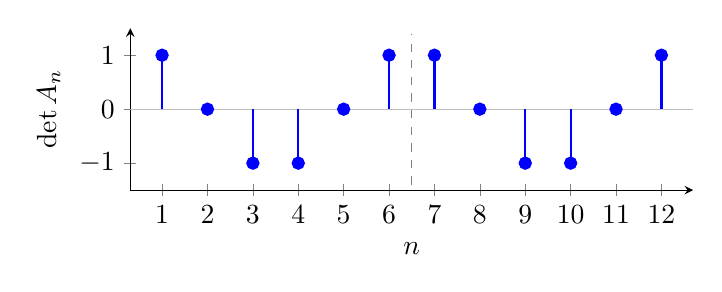
\begin{tikzpicture}
    \begin{axis}[width=0.72\textwidth,height=0.3\textwidth,xmin=0.3,xmax=12.7,ymin=-1.5,ymax=1.5,
        xtick={1,...,12},ytick={-1,0,1},xlabel={$n$},ylabel={$\det A_n$},axis lines=left]
      \draw[gray!50] (axis cs:0.3,0) -- (axis cs:12.7,0);
      \draw[dashed,gray] (axis cs:6.5,-1.4) -- (axis cs:6.5,1.4);
      \addplot[ycomb,blue,thick,mark=*,mark options={fill=blue}] coordinates
        {(1,1) (2,0) (3,-1) (4,-1) (5,0) (6,1) (7,1) (8,0) (9,-1) (10,-1) (11,0) (12,1)};
    \end{axis}
  \end{tikzpicture}
  \caption{Determinants of the tridiagonal matrices of ones. The recursion
  $|A_n|=|A_{n-1}|-|A_{n-2}|$ from the cofactor expansion forces period $6$ (dashed line: one
  period).}
  \label{fig:u21-period}
\end{figure}

\subsection{Exercises}

\begin{exercise}\label{ex:u21-cycle}
Compute the determinant of
\[
  A=\begin{bmatrix}0&0&0&1\\1&0&0&0\\0&1&0&0\\0&0&1&0\end{bmatrix}.
\]
Which method do you prefer here, and why?
\end{exercise}

\begin{solution}
The big formula has a single nonzero term, from the permutation $(4,1,2,3)$, with product
$1$. Moving row~1 to the bottom takes three exchanges (rows 1--2, 2--3, 3--4), which turns $A$
into $I$; the permutation is odd, so $\det A=-1$. Cofactors along row~1 give the same with no
searching: the only nonzero entry is $a_{14}=1$, whose minor (rows 2--4, columns 1--3) is $I_3$,
so $\det A=(-1)^{1+4}\cdot 1=-1$. With a single $1$ in each row, either method beats
elimination.
\end{solution}

\begin{exercise}\label{ex:u21-pascal}
The symmetric Pascal matrices have determinant $1$; for instance
$\det\left[\begin{smallmatrix}1&1&1&1\\1&2&3&4\\1&3&6&10\\1&4&10&20\end{smallmatrix}\right]=1$.
Explain why subtracting $1$ from the $(n,n)$ entry (here $20\to 19$) makes the determinant
$0$.
\end{exercise}

\begin{solution}
By linearity in the last row, the new determinant is the old one plus the determinant of the
matrix whose last row is $(0,\dots,0,-1)$. Expanding that matrix along its last row gives
$(-1)\cdot C_{nn}=-\det(\text{Pascal matrix of size }n-1)=-1$, because $(-1)^{n+n}=+1$. So the
determinant drops from $1$ to $1-1=0$. In the example the cofactor is
$\det\left[\begin{smallmatrix}1&1&1\\1&2&3\\1&3&6\end{smallmatrix}\right]=1$.
\end{solution}

\begin{exercise}\label{ex:u21-cyclic5}
Find the determinant of the $5\times 5$ matrix with $x$ on the diagonal, $y$ just to the
right of the diagonal in rows~1--4, $y$ in position $(5,1)$, and zeros elsewhere:
\[
  A=\begin{bmatrix}x&y&0&0&0\\0&x&y&0&0\\0&0&x&y&0\\0&0&0&x&y\\y&0&0&0&x\end{bmatrix}.
\]
\end{exercise}

\begin{solution}
Expand down column~1, which has only $a_{11}=x$ and $a_{51}=y$. Deleting row~1 and column~1
leaves an upper triangular matrix with $x$'s on its diagonal, determinant $x^4$. Deleting
row~5 and column~1 leaves a lower triangular matrix with $y$'s on its diagonal, determinant
$y^4$, and the sign is $(-1)^{5+1}=+1$. Hence $\det A=x\cdot x^4+y\cdot y^4=x^5+y^5$.
\end{solution}

\begin{exercise}\label{ex:u21-allY}
Find the determinant of the $5\times 5$ matrix $B$ with $x$ on the diagonal and $y$ in every
other position.
\end{exercise}

\begin{solution}
Add rows 2--5 to row~1 (property 5, no change): every entry of row~1 becomes $x+4y$. Factor
it out (property 3a), leaving a row of ones. Now subtract $y$ times this row of ones from each of
rows 2--5. Row $k$ had $y$ in every position except $x$ in position $k$, so it becomes $0$
everywhere except $x-y$ in position $k$. The result is upper
triangular with diagonal $1,\,x-y,\,x-y,\,x-y,\,x-y$, so
\[
  \det B=(x+4y)(x-y)^4 .
\]
Check: for $y=0$ this is $x^5=\det(xI)$, and for $x=y$ all rows are equal and the determinant
is $0$.
\end{solution}

% unit: u22
% sources: sources/086-cramer-s-rule-inverse-matrix-and-volume.txt, sources/039-lecture-20-cramer-s-rule-inverse-matrix-and-volume.txt, sources/191-mit18-06scf11-ses2-7sum-pdf-download-file.txt, sources/040-problem-solving-determinants-and-volume.txt, sources/192-mit18-06scf11-ses2-7prob-pdf-download-file.txt, sources/193-mit18-06scf11-ses2-7sol-pdf-download-file.txt
\section{Cramer's rule, inverse matrix and volume}\label{sec:u22}

The last two sections built the determinant from three properties and found two formulas
for it: the big formula with $n!$ terms and the cofactor expansion
(Section~\ref{sec:u21}). This section puts the determinant to work. The cofactor expansion
turns into an explicit formula for $A^{-1}$; applied to $\vb{b}$ that formula becomes
Cramer's rule for the solution of $A\vb{x}=\vb{b}$; and the absolute value $|\det A|$ turns
out to be a volume. Elimination remains the way to compute. What these formulas give
instead is \emph{algebra}: the answer written in terms of the entries, which shows how it
depends on them.

\subsection{The cofactor matrix gives \texorpdfstring{\(A^{-1}\)}{the inverse}}

Start from the $2\times 2$ inverse we already know:
\[
  \begin{bmatrix} a & b\\ c & d\end{bmatrix}^{-1}
  =\frac{1}{ad-bc}\begin{bmatrix} d & -b\\ -c & a\end{bmatrix}.
\]
We divide by the determinant, which is exactly what fails when $A$ is singular. The entries
of the matrix on the right are cofactors: $d$ is the cofactor of $a$ (strike out row~1 and
column~1), and $-b$ is the cofactor of $c$ (strike out row~2 and column~1, and attach the
sign $(-1)^{2+1}$). Notice that the cofactor of $c$, which sits in position $(2,1)$, appears
in position $(1,2)$. The cofactors are transposed.

\begin{definition}[Cofactor matrix]\label{def:u22-cofactor}
Let $A$ be $n\times n$ and let $M_{ij}$ be the $(n-1)\times(n-1)$ matrix left when row $i$
and column $j$ of $A$ are removed. The cofactor of $a_{ij}$ is
$C_{ij}=(-1)^{i+j}\det M_{ij}$, and the \emph{cofactor matrix} is $C=(C_{ij})$. Its
transpose $C\T$ is sometimes called the adjugate of $A$.
\end{definition}

Each cofactor is a sum of products of $n-1$ entries, while $\det A$ is a sum of products of
$n$ entries. So a formula $A^{-1}=C\T/\det A$ has the right ``degree'': entries of $A^{-1}$
behave like $1/(\text{entry of }A)$. For a general $3\times 3$ matrix with rows
$(a,b,c)$, $(d,e,f)$, $(g,h,i)$, the $(1,1)$ entry of $A^{-1}$ should be
$(ei-fh)/\det A$. The theorem says this pattern holds for every entry and every $n$.

\begin{theorem}[Inverse from cofactors]\label{thm:u22-inverse}
For every square matrix $A$,
\[
  A\,C\T=(\det A)\,I .
\]
Consequently, if $\det A\neq 0$ then $A^{-1}=\dfrac{1}{\det A}\,C\T$, that is,
$(A^{-1})_{ij}=C_{ji}/\det A$.
\end{theorem}

\begin{proof}
The $(i,k)$ entry of $A\,C\T$ is row $i$ of $A$ times column $k$ of $C\T$, which is row $k$
of $C$:
\[
  (A\,C\T)_{ik}=\sum_{j=1}^{n} a_{ij}\,C_{kj}.
\]
\emph{Diagonal entries} ($k=i$). The sum $\sum_j a_{ij}C_{ij}$ is the cofactor expansion of
$\det A$ along row $i$ (Section~\ref{sec:u21}). So every diagonal entry equals $\det A$.

\emph{Off-diagonal entries} ($k\neq i$). Let $A^{*}$ be the matrix $A$ with row $k$
replaced by a copy of row $i$. Then $A^{*}$ has two equal rows, so $\det A^{*}=0$. Expand
$\det A^{*}$ along its row $k$. The entries of that row are $a_{i1},\dots,a_{in}$, and the
cofactors of row $k$ of $A^{*}$ are the same as those of $A$, because they are computed after
deleting row $k$, the only row where $A$ and $A^{*}$ differ. Hence
\[
  0=\det A^{*}=\sum_{j} a_{ij}\,C_{kj}=(A\,C\T)_{ik}.
\]
So $A\,C\T$ has $\det A$ on its diagonal and zeros elsewhere. If $\det A\neq 0$, dividing
by $\det A$ gives $A\,(C\T/\det A)=I$, and a one-sided inverse of a square matrix is its
inverse.
\end{proof}

In the $2\times 2$ case the off-diagonal computation is visible: row~1 of $A$ is $(a,b)$,
the cofactors of row~2 are $(-b,a)$, and $a(-b)+b(a)=0$ is the determinant of the matrix
with two equal rows $\left[\begin{smallmatrix} a&b\\ a&b\end{smallmatrix}\right]$.

\begin{example}[A $3\times 3$ inverse by cofactors]\label{ex:u22-cofactors}
Let
\[
  A=\begin{bmatrix} 1&1&4\\ 1&2&2\\ 1&2&5\end{bmatrix}.
\]
The nine cofactors, each a signed $2\times 2$ determinant, are
\begin{align*}
C_{11}&=+(2\cdot5-2\cdot2)=6, & C_{12}&=-(1\cdot5-2\cdot1)=-3, & C_{13}&=+(1\cdot2-2\cdot1)=0,\\
C_{21}&=-(1\cdot5-4\cdot2)=3, & C_{22}&=+(1\cdot5-4\cdot1)=1, & C_{23}&=-(1\cdot2-1\cdot1)=-1,\\
C_{31}&=+(1\cdot2-4\cdot2)=-6, & C_{32}&=-(1\cdot2-4\cdot1)=2, & C_{33}&=+(1\cdot2-1\cdot1)=1.
\end{align*}
Multiplying $A$ by $C\T$,
\[
  A\,C\T=\begin{bmatrix} 1&1&4\\ 1&2&2\\ 1&2&5\end{bmatrix}
  \begin{bmatrix} 6&3&-6\\ -3&1&2\\ 0&-1&1\end{bmatrix}
  =\begin{bmatrix} 3&0&0\\ 0&3&0\\ 0&0&3\end{bmatrix}=3I,
\]
so $\det A=3$ and
\[
  A^{-1}=\frac13\begin{bmatrix} 6&3&-6\\ -3&1&2\\ 0&-1&1\end{bmatrix}
  =\begin{bmatrix} 2&1&-2\\ -1&\tfrac13&\tfrac23\\ 0&-\tfrac13&\tfrac13\end{bmatrix}.
\]
One more question the formula answers instantly: if the entry $a_{13}=4$ is changed to
$100$, the determinant does not change, because $\det A=a_{11}C_{11}+a_{12}C_{12}+a_{13}C_{13}$
and $C_{13}=0$. (The inverse does change: the cofactors in rows~2 and~3 involve $a_{13}$.)
\end{example}

\subsection{Cramer's rule}

If $A$ is invertible, the solution of $A\vb{x}=\vb{b}$ is
$\vb{x}=A^{-1}\vb{b}=C\T\vb{b}/\det A$. Cramer noticed that each component of $C\T\vb{b}$ is
itself a determinant.

\begin{theorem}[Cramer's rule]\label{thm:u22-cramer}
Let $A$ be $n\times n$ with $\det A\neq 0$, and let $B_j$ be the matrix $A$ with its column
$j$ replaced by $\vb{b}$. Then the solution of $A\vb{x}=\vb{b}$ is
\[
  x_j=\frac{\det B_j}{\det A},\qquad j=1,\dots,n.
\]
\end{theorem}

\begin{proof}
By Theorem~\ref{thm:u22-inverse}, $x_j=(C\T\vb{b})_j/\det A$ and
$(C\T\vb{b})_j=\sum_{i} C_{ij}\,b_i$. Now expand $\det B_j$ down its column $j$, which holds
$b_1,\dots,b_n$. The cofactor of position $(i,j)$ in $B_j$ is computed after deleting
column $j$, so it ignores $\vb{b}$ and equals the cofactor $C_{ij}$ of $A$. Therefore
$\det B_j=\sum_i b_i\,C_{ij}=(C\T\vb{b})_j$.
\end{proof}

\begin{example}[Cramer's rule on a $3\times 3$ system]\label{ex:u22-cramer}
Solve $A\vb{x}=\vb{b}$ with $A$ from Example~\ref{ex:u22-cofactors} and
$\vb{b}=(5,2,5)$. We know $\det A=3$. Replacing one column at a time,
\[
  \det B_1=\begin{vmatrix} 5&1&4\\ 2&2&2\\ 5&2&5\end{vmatrix}=6,\qquad
  \det B_2=\begin{vmatrix} 1&5&4\\ 1&2&2\\ 1&5&5\end{vmatrix}=-3,\qquad
  \det B_3=\begin{vmatrix} 1&1&5\\ 1&2&2\\ 1&2&5\end{vmatrix}=3 .
\]
For instance, expanding $\det B_1$ along row~1 gives
$5(10-4)-1(10-10)+4(4-10)=30-0-24=6$. Hence
$\vb{x}=(6/3,\,-3/3,\,3/3)=(2,-1,1)$. Check: $A(2,-1,1)=(2-1+4,\;2-2+2,\;2-2+5)=(5,2,5)$.
The same answer comes from $\vb{x}=C\T\vb{b}/3$:
$C\T\vb{b}=(30+6-30,\;-15+2+10,\;0-2+5)=(6,-3,3)$.
\end{example}

\begin{remark}[Formula versus algorithm]
Cramer's rule needs $n+1$ determinants of size $n$. Computed by elimination each costs about
$n^{3}/3$ operations, so the rule costs about $n^{4}/3$, against $n^{3}/3$ for solving the
system once by elimination; computed by the big formula it is hopeless. Software never uses
it. Its value is theoretical: it shows that each $x_j$ is a ratio of polynomials in the
entries of $A$ and $\vb{b}$, so the solution depends smoothly on the data wherever
$\det A\neq 0$, and it shows exactly how $\det A$ appears in every denominator.
\end{remark}

\begin{trap}
The inverse is $C\T/\det A$, not $C/\det A$. The cofactors of \emph{row}~$i$ of $A$ fill
\emph{column}~$i$ of $A^{-1}$. A quick test: for
$\left[\begin{smallmatrix} a&b\\ c&d\end{smallmatrix}\right]$ the $(1,2)$ entry of the
inverse must be $-b/(ad-bc)$, which is the cofactor of $c$, not of $b$. Also remember the
checkerboard signs $(-1)^{i+j}$; forgetting them is the other common error.
\end{trap}

\subsection{The determinant is a volume}

Take the rows of an $n\times n$ matrix $A$ as $n$ edges leaving the origin and complete
them to a box: the parallelogram ($n=2$), the parallelepiped ($n=3$), or its analogue in
$\R^{n}$, consisting of all points $t_1\vb{r}_1+\dots+t_n\vb{r}_n$ with $0\le t_i\le 1$.
The claim of this subsection is that the volume of that box is $|\det A|$.

We use only these geometric facts about volume. (V1) A rectangular box whose edges point
along the coordinate axes, with lengths $\ell_1,\dots,\ell_n$, has volume
$\ell_1\cdots\ell_n$. (V2) Listing the edges in another order gives the same box. (V3)
Volume is base times height: the box sits on the base spanned by $n-1$ of its edges, and its
height is the distance of the last edge's tip from that base. (V4) If the edges are dependent,
the box lies in a hyperplane and has volume $0$.

\begin{theorem}[Determinant and volume]\label{thm:u22-volume}
The box whose edges are the rows of $A$ has volume $|\det A|$. The same holds for the box
built on the columns, since $\det A\T=\det A$.
\end{theorem}

\begin{proof}
If $A$ is singular its rows are dependent, so the volume is $0=|\det A|$ by (V4).
Suppose $A$ is invertible. Elimination with row exchanges, followed by elimination upward,
reduces $A$ to a diagonal matrix $D=\operatorname{diag}(d_1,\dots,d_n)$ with nonzero
entries, using two kinds of steps (no row is ever rescaled).

\emph{Subtract $c$ times row $j$ from row $i$.} The determinant is unchanged (property~5 in
Section~\ref{sec:u20}). The box is sheared but its volume is unchanged: take as base the
face spanned by the other $n-1$ rows, which do not move. Row $i$ changes by a multiple of
row $j$, which lies in that base, so the tip of row $i$ moves parallel to the base and the
height stays the same. By (V3) the volume is unchanged.

\emph{Exchange two rows.} The determinant changes sign, so $|\det A|$ is unchanged, and by
(V2) the box is the same.

So both $|\det A|$ and the volume are unchanged at every step, and at the end both equal
$|d_1d_2\cdots d_n|$: the determinant of the diagonal matrix $D$ is the product of its
diagonal entries, and the box of $D$ is a rectangular box with edge lengths
$|d_1|,\dots,|d_n|$ along the axes (V1).
\end{proof}

The lecture argues differently but equivalently: the volume of the box satisfies the three
defining properties of $|\det|$. The unit cube ($A=I$) has volume $1$; exchanging two edges
does not change the box; stretching one edge by $t$ multiplies the volume by $|t|$; and
splitting one edge as a sum splits the volume (when the two pieces lie on the same side of the
base). The shear step in the proof is the geometric heart of the linearity property. The sign
of $\det A$ also means something: it records whether the edges form a right-handed or a
left-handed system, and exchanging two edges reverses the handedness.

A good test case is an orthogonal matrix $Q$. Its rows are perpendicular unit vectors, so its
box is a unit cube turned in space, with volume $1$. The determinant agrees: from
$Q\T Q=I$ and the product rule, $(\det Q\T)(\det Q)=(\det Q)^{2}=1$, so $\det Q=\pm 1$.

\begin{figure}[ht]\centering
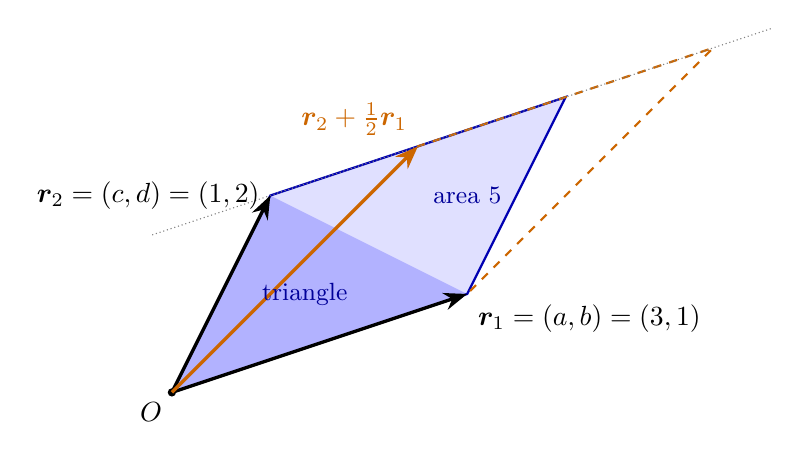
\begin{tikzpicture}[scale=1.25,>=Stealth]
  % original parallelogram on r1=(3,1), r2=(1,2)
  \fill[blue!12] (0,0) -- (3,1) -- (4,3) -- (1,2) -- cycle;
  \fill[blue!30] (0,0) -- (3,1) -- (1,2) -- cycle;
  \draw[thick,blue!70!black] (0,0) -- (3,1) -- (4,3) -- (1,2) -- cycle;
  % sheared parallelogram on r1 and r2 + r1/2 = (2.5,2.5)
  \draw[thick,dashed,orange!80!black] (0,0) -- (3,1) -- (5.5,3.5) -- (2.5,2.5) -- cycle;
  % line through the tip of r2, parallel to r1
  \draw[gray,densely dotted] (-0.2,1.6) -- (6.1,3.7);
  \fill (0,0) circle (1.2pt) node[below left] {$O$};
  \draw[->,very thick] (0,0) -- (3,1) node[below right] {$\vb{r}_1=(a,b)=(3,1)$};
  \draw[->,very thick] (0,0) -- (1,2) node[left] {$\vb{r}_2=(c,d)=(1,2)$};
  \draw[->,very thick,orange!80!black] (0,0) -- (2.5,2.5) node[above left] {$\vb{r}_2+\tfrac12\vb{r}_1$};
  \node[blue!60!black] at (1.35,1.0) {\small triangle};
  \node[blue!60!black] at (3.0,2.0) {\small area $5$};
\end{tikzpicture}
\caption{The parallelogram with edges $\vb{r}_1=(3,1)$ and $\vb{r}_2=(1,2)$ has area
$|ad-bc|=|3\cdot 2-1\cdot 1|=5$, and the shaded triangle is half of it. Adding
$\tfrac12\vb{r}_1$ to $\vb{r}_2$ (a row operation) moves the tip along the dotted line
parallel to $\vb{r}_1$: the dashed parallelogram has the same base and height, hence the
same area, just as the determinant is unchanged.}
\label{fig:u22-area}
\end{figure}

\subsection{Areas and volumes from coordinates}

Theorem~\ref{thm:u22-volume} is a formula that needs no lengths, angles or heights, only
coordinates. In the plane, the parallelogram with edges $(a,b)$ and $(c,d)$ has area
$|ad-bc|$, and the triangle with vertices $(0,0)$, $(a,b)$, $(c,d)$ has half that area
(Figure~\ref{fig:u22-area}). For a triangle placed anywhere:

\begin{proposition}[Area of a triangle]\label{prop:u22-triangle}
The triangle with vertices $(x_1,y_1)$, $(x_2,y_2)$, $(x_3,y_3)$ has area
\[
  \frac12\left|\det\begin{bmatrix} x_1&y_1&1\\ x_2&y_2&1\\ x_3&y_3&1\end{bmatrix}\right| .
\]
\end{proposition}

\begin{proof}
Subtract row~1 from rows~2 and~3; the determinant does not change. The last column becomes
$(1,0,0)$, and expanding along it leaves
\[
  \det\begin{bmatrix} x_2-x_1 & y_2-y_1\\ x_3-x_1 & y_3-y_1\end{bmatrix}.
\]
The row operations translated the triangle so that its first vertex is at the origin; its
other vertices are now the two edge vectors, and half the parallelogram area is the triangle
area.
\end{proof}

For example, the triangle with vertices $(1,1)$, $(4,2)$, $(2,5)$ has edges $(3,1)$ and
$(1,4)$ from the first vertex, so its area is $\tfrac12|3\cdot4-1\cdot1|=\tfrac{11}{2}$. A
zero determinant means the three points are collinear.

\begin{example}[Volume of a tetrahedron]\label{ex:u22-tetra}
A tetrahedron $T$ has one vertex at the origin $O$ and the others at
$A_1=(2,2,-1)$, $A_2=(1,3,0)$ and $A_3=(-1,1,4)$. Find its volume. Then keep $A_1$ and
$A_2$, move the apex to $A_3'=(-201,-199,104)$, and find the new volume.

\emph{Relate $T$ to a box.} Let $P$ be the parallelepiped on the edges $OA_1$, $OA_2$,
$OA_3$. Take the triangle $OA_1A_2$ as the base of $T$ and the parallelogram on $OA_1$,
$OA_2$ as the base of $P$; the parallelogram has twice the area of the triangle, and both
solids have the same height $h$ (the distance from $A_3$ to that plane). So
\[
  \operatorname{vol}(T)=\tfrac13(\text{area of triangle})\,h
  =\tfrac16(\text{area of parallelogram})\,h=\tfrac16\operatorname{vol}(P).
\]
\emph{Compute.} By Theorem~\ref{thm:u22-volume},
\[
  \operatorname{vol}(P)=\left|\det\begin{bmatrix} 2&2&-1\\ 1&3&0\\ -1&1&4\end{bmatrix}\right|
  =\bigl|2(12-0)-2(4-0)+(-1)(1+3)\bigr|=|24-8-4|=12,
\]
so $\operatorname{vol}(T)=12/6=2$.

\emph{Move the apex.} Notice that $A_3'=A_3-100A_1$: indeed
$(-1,1,4)-100(2,2,-1)=(-201,-199,104)$. In the matrix this is the row operation ``subtract
$100$ times row~1 from row~3'', which leaves the determinant at $12$. So the long, needle-like
tetrahedron still has volume $2$. Geometrically, the apex moved parallel to the edge $OA_1$,
which lies in the base plane, so the height did not change.
\end{example}

\subsection{Exercises}

\begin{exercise}[Spherical coordinates]\label{exr:u22-spherical}
Spherical coordinates $(\rho,\phi,\theta)$ are defined by
\[
  x=\rho\sin\phi\cos\theta,\qquad y=\rho\sin\phi\sin\theta,\qquad z=\rho\cos\phi .
\]
Find the $3\times3$ matrix of partial derivatives of $(x,y,z)$ with respect to
$(\rho,\phi,\theta)$ and show that its determinant is $J=\rho^{2}\sin\phi$. Explain why
$\rho^{2}\sin\phi\,d\rho\,d\phi\,d\theta$ is the volume of a small coordinate box.
\end{exercise}
\begin{solution}
The rows are the partial derivatives of $x$, $y$, $z$:
\[
  J=\det\begin{bmatrix}
  \sin\phi\cos\theta & \rho\cos\phi\cos\theta & -\rho\sin\phi\sin\theta\\
  \sin\phi\sin\theta & \rho\cos\phi\sin\theta & \rho\sin\phi\cos\theta\\
  \cos\phi & -\rho\sin\phi & 0
  \end{bmatrix}.
\]
Expand along the bottom row (cofactor signs $+,-,+$; the last entry is $0$):
\begin{align*}
J&=\cos\phi\,\bigl(\rho^{2}\cos\phi\sin\phi\cos^{2}\theta+\rho^{2}\cos\phi\sin\phi\sin^{2}\theta\bigr)
 +\rho\sin\phi\,\bigl(\rho\sin^{2}\phi\cos^{2}\theta+\rho\sin^{2}\phi\sin^{2}\theta\bigr)\\
&=\rho^{2}\cos^{2}\phi\sin\phi+\rho^{2}\sin^{3}\phi
 =\rho^{2}\sin\phi\,(\cos^{2}\phi+\sin^{2}\phi)=\rho^{2}\sin\phi .
\end{align*}
Small changes $d\rho$, $d\phi$, $d\theta$ move the point by the three columns of this matrix
times $d\rho$, $d\phi$, $d\theta$. These three small vectors are the edges of the tiny
coordinate box, so by Theorem~\ref{thm:u22-volume} its volume is
$|J|\,d\rho\,d\phi\,d\theta=\rho^{2}\sin\phi\,d\rho\,d\phi\,d\theta$ (here $0\le\phi\le\pi$, so
$\sin\phi\ge0$).
\end{solution}

\begin{exercise}[Integer inverses]\label{exr:u22-integer}
Suppose $A$ has integer entries. Show that $A^{-1}$ has integer entries if $\det A=\pm1$,
and that conversely, if both $A$ and $A^{-1}$ have integer entries, then $\det A=\pm1$.
Find the inverse of $\left[\begin{smallmatrix} 2&3\\ 1&2\end{smallmatrix}\right]$.
\end{exercise}
\begin{solution}
Every cofactor is a sum of products of integers, so $C\T$ has integer entries; if
$\det A=\pm1$ then $A^{-1}=\pm C\T$ is an integer matrix. Conversely, $\det A$ and
$\det A^{-1}$ are integers (sums of products of integers) and their product is
$\det(AA^{-1})=\det I=1$, so both are $\pm1$. For the example, $\det A=4-3=1$ and
$A^{-1}=C\T=\left[\begin{smallmatrix} 2&-3\\ -1&2\end{smallmatrix}\right]$; indeed
$\left[\begin{smallmatrix} 2&3\\ 1&2\end{smallmatrix}\right]
\left[\begin{smallmatrix} 2&-3\\ -1&2\end{smallmatrix}\right]=I$.
\end{solution}

\begin{exercise}[Determinant of the cofactor matrix]\label{exr:u22-detC}
Show that $\det C=(\det A)^{n-1}$ for an invertible $n\times n$ matrix $A$, and check it on
Example~\ref{ex:u22-cofactors}.
\end{exercise}
\begin{solution}
Take determinants in $A\,C\T=(\det A)I$. The right side is a diagonal matrix with $n$ entries
equal to $\det A$, so its determinant is $(\det A)^{n}$. The left side gives
$\det A\cdot\det C\T=\det A\cdot\det C$. Dividing by $\det A\neq0$ gives
$\det C=(\det A)^{n-1}$. In Example~\ref{ex:u22-cofactors}, $n=3$ and $\det A=3$, so
$\det C$ should be $9$. Directly, expanding
$C=\left[\begin{smallmatrix} 6&-3&0\\ 3&1&-1\\ -6&2&1\end{smallmatrix}\right]$ along row~1:
$6(1+2)+3(3-6)+0=18-9=9$.
\end{solution}

\begin{exercise}[Cramer's rule and collinear points]\label{exr:u22-small}
(a) Solve $2x+y=3$, $x+3y=5$ by Cramer's rule.
(b) Use Proposition~\ref{prop:u22-triangle} to decide whether $(1,2)$, $(3,5)$, $(7,11)$
lie on one line.
\end{exercise}
\begin{solution}
(a) $\det A=2\cdot3-1\cdot1=5$, $\det B_1=\left|\begin{smallmatrix} 3&1\\ 5&3\end{smallmatrix}\right|=9-5=4$,
$\det B_2=\left|\begin{smallmatrix} 2&3\\ 1&5\end{smallmatrix}\right|=10-3=7$. So
$x=4/5$, $y=7/5$. Check: $8/5+7/5=3$ and $4/5+21/5=5$.

(b) Subtracting the first row as in the proof of Proposition~\ref{prop:u22-triangle} leaves
$\det\left[\begin{smallmatrix} 2&3\\ 6&9\end{smallmatrix}\right]=18-18=0$. The triangle
has area $0$, so the points are collinear: the edge $(6,9)$ is $3$ times the edge $(2,3)$.
\end{solution}

% unit: u23
% sources: sources/095-eigenvalues-and-eigenvectors.txt, sources/041-lecture-21-eigenvalues-and-eigenvectors.txt, sources/194-mit18-06scf11-ses2-8sum-pdf-download-file.txt, sources/042-problem-solving-eigenvalues-and-eigenvectors.txt, sources/195-mit18-06scf11-ses2-8prob-pdf-download-file.txt, sources/196-mit18-06scf11-ses2-8sol-pdf-download-file.txt
\section{Eigenvalues and eigenvectors}\label{sec:u23}

Up to now a matrix has mostly been the coefficient matrix of a static problem
$A\vb{x}=\vb{b}$. From here on we also think of a square matrix as an operation that is
applied again and again: $A\vb{u}$, $A^{2}\vb{u}$, $A^{3}\vb{u}$, or continuously in time.
For that, the important vectors are the few whose direction $A$ does not change. They and
their stretching factors, the eigenvectors and eigenvalues, occupy most of the rest of the
course. This section says what they are and how to find them; the next sections use them.

\subsection{Vectors that keep their direction}

A matrix acts like a function: in goes $\vb{x}$, out comes $A\vb{x}$. For most vectors the
output points in a new direction. The eigenvectors are the exceptions.

\begin{definition}[Eigenvalue and eigenvector]\label{def:u23-eig}
Let $A$ be $n\times n$. A number $\lambda$ is an \emph{eigenvalue} of $A$ if there is a
\emph{nonzero} vector $\vb{x}$ with
\[
  A\vb{x}=\lambda\vb{x}.
\]
Such an $\vb{x}$ is an \emph{eigenvector} for $\lambda$. The eigenvectors for $\lambda$,
together with $\vb{0}$, form the \emph{eigenspace} $\Nul{A-\lambda I}$.
\end{definition}

``Same direction'' allows $\lambda$ to be negative (the vector reverses), zero, or even
complex. The vector $\vb{0}$ is excluded because $A\vb{0}=\lambda\vb{0}$ for every
$\lambda$ and would tell us nothing. Any nonzero multiple of an eigenvector is again an
eigenvector, so ``the'' eigenvector really means a basis for the eigenspace.

\emph{Eigenvalue zero.} $A\vb{x}=0\vb{x}$ says $\vb{x}$ is a nonzero vector in the nullspace.
So $\lambda=0$ is an eigenvalue exactly when $A$ is singular, and its eigenvectors are the
nonzero vectors of $\Nul{A}$. Among eigenvalues, zero is no longer special.

Before any formulas, two matrices whose eigenvectors we can see from what they do.

\begin{example}[A projection matrix]\label{ex:u23-projection}
Let $P$ project $\R^{3}$ onto the plane $x+y+z=0$. By the formula
$P=I-\vb{n}\vb{n}\T/\vb{n}\T\vb{n}$ with normal $\vb{n}=(1,1,1)$,
\[
  P=\frac13\begin{bmatrix} 2&-1&-1\\ -1&2&-1\\ -1&-1&2\end{bmatrix}.
\]
A vector already in the plane is not moved: $P\vb{x}=\vb{x}$, so every nonzero vector of the
plane is an eigenvector with $\lambda=1$, for example $(1,-1,0)$ and $(1,0,-1)$. A vector
along the normal is projected to zero: $P(1,1,1)=\vb{0}$, so $\vb{n}$ is an eigenvector with
$\lambda=0$. The eigenvalues are $1,1,0$, and the three eigenvectors are independent. A
typical vector such as $\vb{b}=(1,0,0)$ is \emph{not} an eigenvector:
$P\vb{b}=\tfrac13(2,-1,-1)$ points in another direction.
\end{example}

\begin{example}[A permutation matrix]\label{ex:u23-permutation}
$B=\begin{bmatrix} 0&1\\ 1&0\end{bmatrix}$ swaps the two components:
$B(x_1,x_2)=(x_2,x_1)$. The vector $(1,1)$ is unchanged, so it is an eigenvector with
$\lambda=1$. The vector $(1,-1)$ becomes $(-1,1)$, its negative, so it is an eigenvector
with $\lambda=-1$. A matrix with no negative entries can still have a negative eigenvalue.
\end{example}

\subsection{The characteristic equation}

The equation $A\vb{x}=\lambda\vb{x}$ has two unknowns multiplied together, so elimination
cannot be applied to it directly. The trick is to find $\lambda$ first.

\begin{theorem}[Characteristic equation]\label{thm:u23-chareq}
$\lambda$ is an eigenvalue of $A$ if and only if
\[
  \det(A-\lambda I)=0 .
\]
The eigenvectors for $\lambda$ are the nonzero vectors in $\Nul{A-\lambda I}$.
\end{theorem}

\begin{proof}
$A\vb{x}=\lambda\vb{x}$ is the same as $(A-\lambda I)\vb{x}=\vb{0}$. A nonzero solution
exists exactly when $A-\lambda I$ is singular, and a square matrix is singular exactly when
its determinant is zero (Section~\ref{sec:u20}).
\end{proof}

By the big formula, $p(\lambda)=\det(A-\lambda I)$ is a polynomial of degree $n$ in
$\lambda$, the \emph{characteristic polynomial}; its leading term comes from the product of
the diagonal entries and is $(-\lambda)^{n}$. Over the complex numbers it factors as
$p(\lambda)=(\lambda_1-\lambda)(\lambda_2-\lambda)\cdots(\lambda_n-\lambda)$, so an
$n\times n$ matrix has exactly $n$ eigenvalues if repeated roots are counted with their
multiplicity. The recipe is:
\begin{enumerate}
  \item compute $\det(A-\lambda I)$ and find its $n$ roots $\lambda_1,\dots,\lambda_n$;
  \item for each $\lambda_i$, find the nullspace of the singular matrix $A-\lambda_i I$ by
  elimination (give the free variable the value $1$).
\end{enumerate}

\begin{example}[A symmetric $2\times 2$ matrix]\label{ex:u23-31}
Let $A=\begin{bmatrix} 3&1\\ 1&3\end{bmatrix}$. Then
\[
  \det(A-\lambda I)=\begin{vmatrix} 3-\lambda & 1\\ 1 & 3-\lambda\end{vmatrix}
  =(3-\lambda)^{2}-1=\lambda^{2}-6\lambda+8=(\lambda-4)(\lambda-2),
\]
so $\lambda_1=4$ and $\lambda_2=2$. For $\lambda_1=4$:
$A-4I=\left[\begin{smallmatrix} -1&1\\ 1&-1\end{smallmatrix}\right]$, whose nullspace is the
line through $\vb{x}_1=(1,1)$. For $\lambda_2=2$:
$A-2I=\left[\begin{smallmatrix} 1&1\\ 1&1\end{smallmatrix}\right]$, whose nullspace is the
line through $\vb{x}_2=(-1,1)$. Check: $A(1,1)=(4,4)$ and $A(-1,1)=(-2,2)$.
Figure~\ref{fig:u23-stretch} shows the two eigenvector lines.
\end{example}

\begin{figure}[ht]\centering
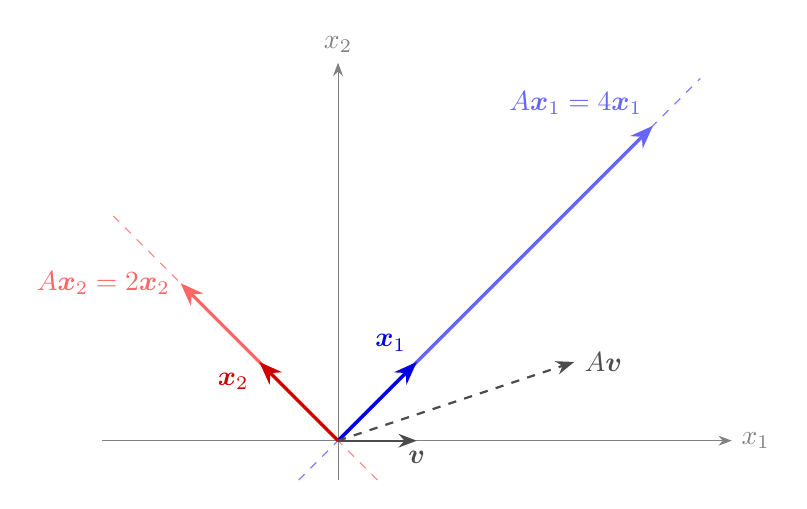
\begin{tikzpicture}[scale=1.0,>=Stealth]
  \draw[->,gray] (-3,0) -- (5,0) node[right] {$x_1$};
  \draw[->,gray] (0,-0.5) -- (0,4.8) node[above] {$x_2$};
  \draw[blue!50,dashed] (-0.5,-0.5) -- (4.6,4.6);
  \draw[red!50,dashed] (0.5,-0.5) -- (-2.9,2.9);
  \draw[->,very thick,blue!60] (0,0) -- (4,4) node[above left] {$A\vb{x}_1=4\vb{x}_1$};
  \draw[->,very thick,blue!90!black] (0,0) -- (1,1) node[above left] {$\vb{x}_1$};
  \draw[->,very thick,red!60] (0,0) -- (-2,2) node[left] {$A\vb{x}_2=2\vb{x}_2$};
  \draw[->,very thick,red!80!black] (0,0) -- (-1,1) node[below left] {$\vb{x}_2$};
  \draw[->,thick,black!70] (0,0) -- (1,0) node[below] {$\vb{v}$};
  \draw[->,thick,black!70,dashed] (0,0) -- (3,1) node[right] {$A\vb{v}$};
\end{tikzpicture}
\caption{For $A=\left[\begin{smallmatrix} 3&1\\ 1&3\end{smallmatrix}\right]$, vectors on the
dashed line through $(1,1)$ are stretched by $\lambda_1=4$ and vectors on the line through
$(-1,1)$ by $\lambda_2=2$, without turning. A typical vector such as $\vb{v}=(1,0)$ is turned:
$A\vb{v}=(3,1)$ is not a multiple of $\vb{v}$.}
\label{fig:u23-stretch}
\end{figure}

The matrix in Example~\ref{ex:u23-31} is $B+3I$, with $B$ the permutation of
Example~\ref{ex:u23-permutation}. Its eigenvalues $4,2$ are those of $B$ (namely $1,-1$)
plus $3$, and its eigenvectors are the same lines. This is a general fact.

\begin{proposition}[Shifting by a multiple of $I$]\label{prop:u23-shift}
If $A\vb{x}=\lambda\vb{x}$, then $(A+cI)\vb{x}=(\lambda+c)\vb{x}$. So $A+cI$ has the
eigenvalues of $A$ shifted by $c$, with the same eigenvectors.
\end{proposition}

\begin{proof}
$(A+cI)\vb{x}=A\vb{x}+c\vb{x}=\lambda\vb{x}+c\vb{x}=(\lambda+c)\vb{x}$.
\end{proof}

\begin{trap}
It is tempting to argue: if $A\vb{x}=\lambda\vb{x}$ and $B\vb{x}=\alpha\vb{x}$ then
$(A+B)\vb{x}=(\lambda+\alpha)\vb{x}$, so eigenvalues add. The flaw is that $A$ and $B$
usually have \emph{different} eigenvectors, and then nothing can be concluded. For
$A=\left[\begin{smallmatrix} 0&1\\ 0&0\end{smallmatrix}\right]$ and
$B=\left[\begin{smallmatrix} 0&0\\ 1&0\end{smallmatrix}\right]$ all four eigenvalues are $0$,
yet $A+B$ has eigenvalues $1$ and $-1$, and $AB=\left[\begin{smallmatrix} 1&0\\ 0&0\end{smallmatrix}\right]$
has eigenvalues $1$ and $0$. Eigenvalues are neither additive nor multiplicative; the shift
$B=cI$ works only because every vector is an eigenvector of $cI$.
\end{trap}

\subsection{Trace and determinant}

In Example~\ref{ex:u23-31} the coefficient $6$ in $\lambda^{2}-6\lambda+8$ is $3+3$, the sum
of the diagonal entries, and the constant $8$ is $\det A$. That is no accident.

\begin{theorem}[Sum and product of the eigenvalues]\label{thm:u23-trace}
Let $\lambda_1,\dots,\lambda_n$ be the eigenvalues of $A$, repeated according to
multiplicity. Then
\[
  \lambda_1+\lambda_2+\dots+\lambda_n=a_{11}+a_{22}+\dots+a_{nn}=\tr A,
  \qquad
  \lambda_1\lambda_2\cdots\lambda_n=\det A .
\]
\end{theorem}

\begin{proof}
Compare two expressions for the characteristic polynomial,
\[
  \det(A-\lambda I)=(\lambda_1-\lambda)(\lambda_2-\lambda)\cdots(\lambda_n-\lambda).
\]
\emph{Product.} Set $\lambda=0$: $\det A=\lambda_1\lambda_2\cdots\lambda_n$.

\emph{Sum.} Look at the coefficient of $\lambda^{n-1}$. On the right it is
$(-1)^{n-1}(\lambda_1+\dots+\lambda_n)$. On the left, use the big formula: each term is a
product of $n$ entries of $A-\lambda I$, one from each row and each column. A term that uses
an off-diagonal entry in position $(i,j)$ cannot also use the diagonal entries of row $i$ or
of column $j$, so it contains at most $n-2$ factors with $\lambda$. Hence only the diagonal
product $(a_{11}-\lambda)\cdots(a_{nn}-\lambda)$ reaches $\lambda^{n-1}$, with coefficient
$(-1)^{n-1}(a_{11}+\dots+a_{nn})$. Equate the two coefficients.
\end{proof}

For a $2\times 2$ matrix this pins the characteristic equation down completely:
\[
  \lambda^{2}-(\tr A)\,\lambda+\det A=0 .
\]
Knowing one eigenvalue, the trace gives the other at once. The two facts are also the
quickest check on a computation: add the eigenvalues and compare with the diagonal.

\begin{example}[Two cities: finding eigenvalues by inspection]\label{ex:u23-markov}
Each year $80\%$ of the people in city~1 stay and $20\%$ move to city~2, while $70\%$ of
city~2 stays and $30\%$ moves to city~1. The populations change by
\[
  A=\begin{bmatrix} 0.8&0.3\\ 0.2&0.7\end{bmatrix}.
\]
Try $\vb{x}_1=(600,400)$:
$A\vb{x}_1=(480+120,\;120+280)=(600,400)$. So $\vb{x}_1$ is an eigenvector with
$\lambda_1=1$. The trace is $0.8+0.7=1.5$, so $\lambda_2=1.5-1=0.5$. The determinant
confirms it: $0.56-0.06=0.5=\lambda_1\lambda_2$. For $\lambda_2$,
$A-0.5I=\left[\begin{smallmatrix} 0.3&0.3\\ 0.2&0.2\end{smallmatrix}\right]$ has nullspace
spanned by $\vb{x}_2=(1,-1)$, and indeed $A(1,-1)=(0.5,-0.5)=0.5\,\vb{x}_2$. The two
eigenvectors are the key to what happens to the populations year after year:
Section~\ref{sec:u24} follows them.
\end{example}

\subsection{Complex eigenvalues}

The $90^{\circ}$ rotation $Q=\begin{bmatrix} 0&-1\\ 1&0\end{bmatrix}$ turns every nonzero
vector, so no real vector can be an eigenvector. The trace and determinant agree that
something is strange: $\lambda_1+\lambda_2=0$ but $\lambda_1\lambda_2=1$, impossible for
real numbers. The characteristic equation settles it:
\[
  \det(Q-\lambda I)=\begin{vmatrix} -\lambda & -1\\ 1 & -\lambda\end{vmatrix}=\lambda^{2}+1=0,
  \qquad \lambda_1=i,\quad \lambda_2=-i .
\]
For $\lambda_1=i$, the nullspace of $Q-iI$ contains $\vb{x}_1=(1,-i)$; check:
$Q(1,-i)=(i,1)=i(1,-i)$. Similarly $\vb{x}_2=(1,i)$ goes with $-i$. A perfectly real matrix
can have complex eigenvalues and eigenvectors.

\begin{proposition}[Conjugate pairs]\label{prop:u23-conj}
If $A$ is real and $A\vb{x}=\lambda\vb{x}$, then $A\bar{\vb{x}}=\bar\lambda\bar{\vb{x}}$.
So the nonreal eigenvalues of a real matrix come in conjugate pairs $a\pm ib$, with conjugate
eigenvectors.
\end{proposition}

\begin{proof}
Take complex conjugates of every entry in $A\vb{x}=\lambda\vb{x}$. Since $\bar A=A$, this
gives $A\bar{\vb{x}}=\bar\lambda\bar{\vb{x}}$, and $\bar{\vb{x}}\neq\vb{0}$.
\end{proof}

How far a matrix is from symmetric decides how complex its eigenvalues can be. Symmetric
matrices ($A\T=A$) have real eigenvalues and perpendicular eigenvectors; this is proved in
Section~\ref{sec:u29}, and the examples $B$ and $\left[\begin{smallmatrix} 3&1\\ 1&3\end{smallmatrix}\right]$
above show it. The rotation $Q$ is antisymmetric ($Q\T=-Q$), the opposite extreme, and its
eigenvalues are purely imaginary.

\subsection{Triangular matrices and repeated eigenvalues}

\begin{proposition}[Triangular matrices]\label{prop:u23-triangular}
The eigenvalues of a triangular matrix are its diagonal entries.
\end{proposition}

\begin{proof}
$A-\lambda I$ is triangular with diagonal entries $a_{ii}-\lambda$, and the determinant of a
triangular matrix is the product of its diagonal entries. So
$\det(A-\lambda I)=(a_{11}-\lambda)\cdots(a_{nn}-\lambda)$, with roots $a_{11},\dots,a_{nn}$.
\end{proof}

Triangular matrices show the one real danger in this subject: a repeated eigenvalue can come
with too few eigenvectors.

\begin{example}[A shortage of eigenvectors]\label{ex:u23-defective}
$A=\begin{bmatrix} 3&1\\ 0&3\end{bmatrix}$ has $\det(A-\lambda I)=(3-\lambda)^{2}$, so
$\lambda_1=\lambda_2=3$. The eigenvectors fill the nullspace of
$A-3I=\left[\begin{smallmatrix} 0&1\\ 0&0\end{smallmatrix}\right]$, which has rank $1$, so
the nullspace is only the line through $(1,0)$. There is no second independent eigenvector.
Compare $3I$, which has the same eigenvalues $3,3$ but for which every nonzero vector is an
eigenvector. A repeated eigenvalue may or may not cost us eigenvectors; Section~\ref{sec:u24}
explains why this matters.
\end{example}

\subsection{Eigenvalues of powers, inverses and polynomials}

Once the eigenvectors of $A$ are known, many related matrices come for free.

\begin{proposition}[Functions of $A$]\label{prop:u23-functions}
Suppose $A\vb{x}=\lambda\vb{x}$. Then $A^{k}\vb{x}=\lambda^{k}\vb{x}$ for $k=1,2,\dots$, and
for any polynomial $p$, $p(A)\vb{x}=p(\lambda)\vb{x}$. If $A$ is invertible, then
$\lambda\neq0$ and $A^{-1}\vb{x}=\lambda^{-1}\vb{x}$.
\end{proposition}

\begin{proof}
$A^{2}\vb{x}=A(\lambda\vb{x})=\lambda A\vb{x}=\lambda^{2}\vb{x}$, and induction gives
$A^{k}\vb{x}=\lambda^{k}\vb{x}$. A polynomial $p(A)=c_0I+c_1A+\dots+c_mA^{m}$ then sends
$\vb{x}$ to $(c_0+c_1\lambda+\dots+c_m\lambda^{m})\vb{x}$. If $A$ is invertible it is not
singular, so $\lambda\neq0$; multiplying $A\vb{x}=\lambda\vb{x}$ by $A^{-1}$ and dividing by
$\lambda$ gives $A^{-1}\vb{x}=\lambda^{-1}\vb{x}$.
\end{proof}

\begin{example}[Eigenvalues of $A^{2}$ and $A^{-1}-I$ without computing them]\label{ex:u23-recitation}
Find the eigenvalues and eigenvectors of $A^{2}$ and of $A^{-1}-I$ for
\[
  A=\begin{bmatrix} 1&2&3\\ 0&1&-2\\ 0&1&4\end{bmatrix}.
\]

By Proposition~\ref{prop:u23-functions} it is enough to find those of $A$. Expand
$\det(A-\lambda I)$ down the first column, which has a single nonzero entry:
\[
  \det(A-\lambda I)=(1-\lambda)\begin{vmatrix} 1-\lambda & -2\\ 1 & 4-\lambda\end{vmatrix}
  =(1-\lambda)(\lambda^{2}-5\lambda+6)=(1-\lambda)(\lambda-2)(\lambda-3).
\]
The eigenvalues are $1,2,3$ (trace check: $1+1+4=6=1+2+3$). The eigenvectors:
\begin{itemize}
  \item $\lambda=1$: $A-I=\left[\begin{smallmatrix} 0&2&3\\ 0&0&-2\\ 0&1&3\end{smallmatrix}\right]$
  has a zero first column, so $x_1$ is free; the last two rows force $x_3=0$, then $x_2=0$.
  Eigenvector $(1,0,0)$.
  \item $\lambda=2$: $A-2I=\left[\begin{smallmatrix} -1&2&3\\ 0&-1&-2\\ 0&1&2\end{smallmatrix}\right]$.
  Row~2 gives $x_2=-2x_3$; row~1 gives $x_1=2x_2+3x_3=-x_3$. With $x_3=1$: $(-1,-2,1)$.
  \item $\lambda=3$: $A-3I=\left[\begin{smallmatrix} -2&2&3\\ 0&-2&-2\\ 0&1&1\end{smallmatrix}\right]$.
  Row~3 gives $x_2=-x_3$; row~1 gives $2x_1=2x_2+3x_3=x_3$. With $x_3=2$: $(1,-2,2)$.
\end{itemize}
These three vectors are eigenvectors of $A^{2}$ with eigenvalues $1,4,9$, and of $A^{-1}-I$
with eigenvalues $\tfrac11-1=0$, $\tfrac12-1=-\tfrac12$ and $\tfrac13-1=-\tfrac23$. We
never squared or inverted a $3\times3$ matrix.
\end{example}

\subsection{Exercises}

\begin{exercise}\label{exr:u23-B012}
A $3\times3$ matrix $B$ has eigenvalues $0$, $1$, $2$. Which of the following can be
determined from this information? Give them where possible.
(a) the rank of $B$; (b) $\det(B\T B)$; (c) the eigenvalues of $B\T B$;
(d) the eigenvalues of $(B^{2}+I)^{-1}$.
\end{exercise}
\begin{solution}
(a) The rank is $2$. Since $0$ is an eigenvalue, $B$ is singular and the rank is at most $2$.
Eigenvectors $\vb{x}_1,\vb{x}_2$ for $\lambda=1,2$ lie in the column space, because
$\vb{x}=B(\vb{x}/\lambda)$ when $\lambda\neq0$. They are independent: if
$\vb{x}_2=c\,\vb{x}_1$ then $2\vb{x}_2=B\vb{x}_2=c\,\vb{x}_1=\vb{x}_2$, impossible for
$\vb{x}_2\neq\vb{0}$. So the rank is at least $2$.

(b) $\det(B\T B)=\det B\T\det B=0\cdot0=0$, since $\det B=0\cdot1\cdot2$.

(c) Not determined. For $B=\operatorname{diag}(0,1,2)$, $B\T B=\operatorname{diag}(0,1,4)$
has eigenvalues $0,1,4$. For the triangular
$B=\left[\begin{smallmatrix} 0&1&0\\ 0&1&0\\ 0&0&2\end{smallmatrix}\right]$, which also has
eigenvalues $0,1,2$, we get
$B\T B=\left[\begin{smallmatrix} 0&0&0\\ 0&2&0\\ 0&0&4\end{smallmatrix}\right]$ with
eigenvalues $0,2,4$.

(d) By Proposition~\ref{prop:u23-functions}, an eigenvector of $B$ with eigenvalue
$\lambda$ is an eigenvector of $B^{2}+I$ with eigenvalue $\lambda^{2}+1\neq0$, hence of its
inverse with eigenvalue $1/(\lambda^{2}+1)$. The eigenvalues are $1$, $\tfrac12$, $\tfrac15$.
\end{solution}

\begin{exercise}\label{exr:u23-ABC}
Find the eigenvalues of
\[
  A=\begin{bmatrix} 1&2&3\\ 0&4&5\\ 0&0&6\end{bmatrix},\qquad
  B=\begin{bmatrix} 0&0&1\\ 0&2&0\\ 3&0&0\end{bmatrix},\qquad
  C=\begin{bmatrix} 2&2&2\\ 2&2&2\\ 2&2&2\end{bmatrix}.
\]
\end{exercise}
\begin{solution}
$A$ is triangular, so its eigenvalues are $1,4,6$
(Proposition~\ref{prop:u23-triangular}). For $B$, expand along the middle row:
\[
  \det(B-\lambda I)=(2-\lambda)\begin{vmatrix} -\lambda & 1\\ 3 & -\lambda\end{vmatrix}
  =(2-\lambda)(\lambda^{2}-3),
\]
so the eigenvalues are $2$, $\sqrt3$, $-\sqrt3$ (check: the sum is $2=\tr B$ and the product
$-6$ equals $\det B=-6$). $C$ has rank $1$, so its nullspace is a plane and $\lambda=0$ is an
eigenvalue twice; the trace $6$ gives the third eigenvalue $6$, with eigenvector $(1,1,1)$.
Directly, $\det(C-\lambda I)=-\lambda^{3}+6\lambda^{2}=-\lambda^{2}(\lambda-6)$.
\end{solution}

\begin{exercise}\label{exr:u23-idempotent}
Show that every eigenvalue of a projection matrix ($P^{2}=P$) is $0$ or $1$.
\end{exercise}
\begin{solution}
If $P\vb{x}=\lambda\vb{x}$ with $\vb{x}\neq\vb{0}$, then by
Proposition~\ref{prop:u23-functions} $\lambda^{2}\vb{x}=P^{2}\vb{x}=P\vb{x}=\lambda\vb{x}$,
so $(\lambda^{2}-\lambda)\vb{x}=\vb{0}$ and $\lambda(\lambda-1)=0$. Example~\ref{ex:u23-projection}
shows both values occurring: the plane gives $\lambda=1$, the normal line $\lambda=0$.
\end{solution}

\begin{exercise}\label{exr:u23-rotation}
Find the eigenvalues and eigenvectors of the rotation through the angle $\theta$,
\[
  R=\begin{bmatrix} \cos\theta & -\sin\theta\\ \sin\theta & \cos\theta\end{bmatrix},
\]
and check Theorem~\ref{thm:u23-trace}.
\end{exercise}
\begin{solution}
$\det(R-\lambda I)=(\cos\theta-\lambda)^{2}+\sin^{2}\theta=\lambda^{2}-2\lambda\cos\theta+1$.
The quadratic formula gives
$\lambda=\cos\theta\pm\sqrt{\cos^{2}\theta-1}=\cos\theta\pm i\sin\theta=e^{\pm i\theta}$.
For $\lambda=e^{i\theta}$, the vector $(1,-i)$ works:
$R(1,-i)=(\cos\theta+i\sin\theta,\;\sin\theta-i\cos\theta)=e^{i\theta}(1,-i)$; the conjugate
$(1,i)$ goes with $e^{-i\theta}$ (Proposition~\ref{prop:u23-conj}). The sum
$e^{i\theta}+e^{-i\theta}=2\cos\theta$ is the trace and the product $1$ is
$\det R=\cos^{2}\theta+\sin^{2}\theta$. For $\theta=90^{\circ}$ this is the matrix $Q$ above,
with eigenvalues $\pm i$. Both eigenvalues have $|\lambda|=1$: a rotation does not change
lengths.
\end{solution}

% unit: u24
% sources: sources/092-diagonalization-and-powers-of-a.txt, sources/043-lecture-22-diagonalization-and-powers-of-a.txt, sources/197-mit18-06scf11-ses2-9sum-pdf-download-file.txt, sources/044-problem-solving-powers-of-a-matrix.txt, sources/198-mit18-06scf11-ses2-9prob-pdf-download-file.txt, sources/199-mit18-06scf11-ses2-9sol-pdf-download-file.txt, short_plan.json (s04)
\section{Diagonalization and powers of \texorpdfstring{\(A\)}{A}}\label{sec:u24}

Section~\ref{sec:u23} found eigenvalues and eigenvectors one at a time. Now we use all of
them at once. Putting the eigenvectors into the columns of a matrix turns $A$ into a
diagonal matrix, and that single factorization makes powers of $A$ easy: $A^{100}$ costs no
more than $A$. Powers of a matrix are what we need for any process that repeats the same
linear step, such as populations that move every year or the Fibonacci numbers.

\subsection{The eigenvector matrix diagonalizes \texorpdfstring{\(A\)}{A}}

\begin{theorem}[Diagonalization]\label{thm:u24-diag}
Suppose the $n\times n$ matrix $A$ has $n$ linearly independent eigenvectors
$\vb{x}_1,\dots,\vb{x}_n$, with $A\vb{x}_i=\lambda_i\vb{x}_i$. Put them in the columns of
the \emph{eigenvector matrix} $X$ and the eigenvalues on the diagonal of the
\emph{eigenvalue matrix} $\Lambda$:
\[
  X=\begin{bmatrix} \vb{x}_1 & \cdots & \vb{x}_n\end{bmatrix},\qquad
  \Lambda=\begin{bmatrix} \lambda_1 & & \\ & \ddots & \\ & & \lambda_n\end{bmatrix}.
\]
Then $AX=X\Lambda$, and since $X$ is invertible,
\[
  X^{-1}AX=\Lambda\qquad\text{and}\qquad A=X\Lambda X^{-1}.
\]
Conversely, if $A=X\Lambda X^{-1}$ with $X$ invertible and $\Lambda$ diagonal, then the
columns of $X$ are $n$ independent eigenvectors of $A$ and the diagonal entries of $\Lambda$
are the matching eigenvalues.
\end{theorem}

\begin{proof}
Multiply a column at a time. Column $j$ of $AX$ is $A\vb{x}_j=\lambda_j\vb{x}_j$. Column $j$
of $X\Lambda$ is $X$ times column $j$ of $\Lambda$, which is $\lambda_j$ times the $j$th
unit vector, so it is $\lambda_j\vb{x}_j$ as well. Hence $AX=X\Lambda$. The columns of $X$ are
independent, so $X^{-1}$ exists; multiplying on the left or on the right by $X^{-1}$ gives
the two forms. Conversely, $A=X\Lambda X^{-1}$ gives $AX=X\Lambda$, whose column $j$ reads
$A\vb{x}_j=\lambda_j\vb{x}_j$; and $\vb{x}_j\neq\vb{0}$ because $X$ is invertible.
\end{proof}

A matrix that can be written this way is called \emph{diagonalizable}. The lectures call the
eigenvector matrix $S$; these notes write $X$, as in the notation table. To remember the
order of the factors, note that $A$ multiplies its eigenvectors, so $X$ stands immediately to
the right of $A$ in $AX=X\Lambda$. The factorization $A=X\Lambda X^{-1}$ joins $A=LU$ from
elimination and $A=QR$ from Gram--Schmidt; unlike those two, it describes what $A$
\emph{does} when it is applied repeatedly.

\begin{example}[Diagonalizing the two-city matrix]\label{ex:u24-diag}
In Section~\ref{sec:u23} the two-city matrix
$A=\left[\begin{smallmatrix} 0.8&0.3\\ 0.2&0.7\end{smallmatrix}\right]$ had eigenvalues $1$
and $0.5$ with eigenvectors along $(600,400)$ and $(1,-1)$. Scale the first to $(3,2)$:
\[
  X=\begin{bmatrix} 3&1\\ 2&-1\end{bmatrix},\qquad
  \Lambda=\begin{bmatrix} 1&0\\ 0&0.5\end{bmatrix},\qquad
  X^{-1}=\frac{1}{-5}\begin{bmatrix} -1&-1\\ -2&3\end{bmatrix}
  =\frac15\begin{bmatrix} 1&1\\ 2&-3\end{bmatrix}.
\]
Check: $X\Lambda=\left[\begin{smallmatrix} 3&0.5\\ 2&-0.5\end{smallmatrix}\right]$ and
\[
  X\Lambda X^{-1}=\frac15\begin{bmatrix} 3+1 & 3-1.5\\ 2-1 & 2+1.5\end{bmatrix}
  =\begin{bmatrix} 0.8&0.3\\ 0.2&0.7\end{bmatrix}=A .
\]
\end{example}

\subsection{Powers of \texorpdfstring{\(A\)}{A}}

Squaring $A=X\Lambda X^{-1}$, the inner $X^{-1}X$ cancels:
$A^{2}=X\Lambda X^{-1}X\Lambda X^{-1}=X\Lambda^{2}X^{-1}$.

\begin{proposition}[Powers]\label{prop:u24-powers}
If $A=X\Lambda X^{-1}$, then $A^{k}=X\Lambda^{k}X^{-1}$ for every $k\ge1$, where
$\Lambda^{k}=\operatorname{diag}(\lambda_1^{k},\dots,\lambda_n^{k})$. So $A^{k}$ has the same
eigenvectors as $A$ and eigenvalues $\lambda_i^{k}$. If $A$ is invertible the same holds for
$k=-1$.
\end{proposition}

\begin{proof}
In the product of $k$ copies of $X\Lambda X^{-1}$, each of the $k-1$ inner pairs
$X^{-1}X$ equals $I$, leaving $X\Lambda^{k}X^{-1}$. A power of a diagonal matrix is
diagonal with the powers of its entries. For $k=-1$, $(X\Lambda X^{-1})^{-1}=X\Lambda^{-1}X^{-1}$,
which exists when no $\lambda_i$ is zero.
\end{proof}

Compare this with $LU$: multiplying $LU$ by itself a hundred times gives a hundred factors
that do not simplify. The eigenvector picture is the one that makes $A^{100}$ transparent.
For the two-city matrix of Example~\ref{ex:u24-diag},
\[
  A^{k}=X\begin{bmatrix} 1&0\\ 0&0.5^{k}\end{bmatrix}X^{-1}
  =\frac15\begin{bmatrix} 3+2(0.5)^{k} & 3-3(0.5)^{k}\\ 2-2(0.5)^{k} & 2+3(0.5)^{k}\end{bmatrix}
  \;\longrightarrow\;\begin{bmatrix} 0.6&0.6\\ 0.4&0.4\end{bmatrix}\quad(k\to\infty).
\]
At $k=1$ this gives back $A$. The question ``does $A^{k}$ go to zero?'' cannot be answered
from the pivots, but the eigenvalues answer it at once.

\begin{theorem}[When powers go to zero]\label{thm:u24-stable}
Let $A$ be diagonalizable with eigenvalues $\lambda_1,\dots,\lambda_n$. Then $A^{k}\to0$ as
$k\to\infty$ if and only if $|\lambda_i|<1$ for every $i$.
\end{theorem}

\begin{proof}
If every $|\lambda_i|<1$, then each $\lambda_i^{k}\to0$, so $\Lambda^{k}\to0$ and
$A^{k}=X\Lambda^{k}X^{-1}\to0$ because $X$ and $X^{-1}$ do not change with $k$. Conversely,
if some $|\lambda_j|\ge1$, then $A^{k}\vb{x}_j=\lambda_j^{k}\vb{x}_j$ has length
$|\lambda_j|^{k}\|\vb{x}_j\|\ge\|\vb{x}_j\|>0$ for every $k$, so $A^{k}$ does not go to zero.
\end{proof}

The absolute value matters because eigenvalues can be negative or complex. The theorem stays
true for matrices that cannot be diagonalized (Exercise~\ref{exr:u24-jordan} shows one), but
that proof needs the Jordan form of Section~\ref{sec:u32}.

\subsection{Which matrices can be diagonalized?}

Everything above assumed $n$ independent eigenvectors. Distinct eigenvalues guarantee them.

\begin{theorem}[Distinct eigenvalues give independent eigenvectors]\label{thm:u24-distinct}
Eigenvectors $\vb{x}_1,\dots,\vb{x}_k$ that belong to distinct eigenvalues
$\lambda_1,\dots,\lambda_k$ are linearly independent. In particular, an $n\times n$ matrix
with $n$ distinct eigenvalues is diagonalizable.
\end{theorem}

\begin{proof}
Induction on $k$; one nonzero vector is independent. Suppose the statement holds for $k-1$
vectors, and $c_1\vb{x}_1+\dots+c_k\vb{x}_k=\vb{0}$. Multiply by $A-\lambda_kI$. Since
$(A-\lambda_kI)\vb{x}_i=(\lambda_i-\lambda_k)\vb{x}_i$, the last term disappears:
\[
  c_1(\lambda_1-\lambda_k)\vb{x}_1+\dots+c_{k-1}(\lambda_{k-1}-\lambda_k)\vb{x}_{k-1}=\vb{0}.
\]
By the induction hypothesis every coefficient is zero, and $\lambda_i\neq\lambda_k$, so
$c_1=\dots=c_{k-1}=0$. Then $c_k\vb{x}_k=\vb{0}$ forces $c_k=0$.
\end{proof}

A random matrix has distinct eigenvalues (MATLAB's \texttt{eig(rand(10))} will show ten
different numbers), so ``most'' matrices are diagonalizable. Trouble can come only from
repeated eigenvalues, and then we must count.

\begin{definition}[Algebraic and geometric multiplicity]\label{def:u24-mult}
The \emph{algebraic multiplicity} of an eigenvalue $\lambda$ is the number of times it is a
root of $\det(A-\lambda I)$. Its \emph{geometric multiplicity} is the number of independent
eigenvectors, $\dim\Nul{A-\lambda I}$.
\end{definition}

The geometric multiplicity is at least $1$ and never exceeds the algebraic one (a proof uses
the similar matrices of Section~\ref{sec:u32}). Eigenvectors from different eigenspaces
combine independently, by the same argument as Theorem~\ref{thm:u24-distinct}, so $A$ is
diagonalizable exactly when the geometric multiplicities add up to $n$, that is, when every
eigenvalue has as many independent eigenvectors as its algebraic multiplicity.

\begin{example}[Repeated eigenvalues, two outcomes]\label{ex:u24-repeated}
The $n\times n$ identity has the eigenvalue $1$ repeated $n$ times, and every nonzero vector
is an eigenvector; any invertible $X$ gives $X^{-1}IX=I=\Lambda$. In contrast,
$A=\left[\begin{smallmatrix} 2&1\\ 0&2\end{smallmatrix}\right]$ has
$\det(A-\lambda I)=(2-\lambda)^{2}$, algebraic multiplicity $2$, but
$A-2I=\left[\begin{smallmatrix} 0&1\\ 0&0\end{smallmatrix}\right]$ has a one-dimensional
nullspace spanned by $(1,0)$: geometric multiplicity $1$. There is no invertible $X$ with
$X^{-1}AX$ diagonal; indeed the only diagonal candidate is $\Lambda=2I$, and
$X(2I)X^{-1}=2I\neq A$.
\end{example}

\begin{trap}
Diagonalizable and invertible are unrelated properties. Invertibility is about the
eigenvalues (none is $0$); diagonalizability is about the eigenvectors (enough of them).
$\left[\begin{smallmatrix} 2&1\\ 0&2\end{smallmatrix}\right]$ is invertible but not
diagonalizable; $\left[\begin{smallmatrix} 1&0\\ 0&0\end{smallmatrix}\right]$ is
diagonalizable but singular. Also, $X$ is not unique: its columns can be rescaled and
reordered, as long as $\Lambda$ is reordered the same way.
\end{trap}

\subsection{Difference equations \texorpdfstring{\(\vb{u}_{k+1}=A\vb{u}_k\)}{u(k+1) = A u(k)}}

Start with a vector $\vb{u}_0$ and apply the same step over and over:
$\vb{u}_1=A\vb{u}_0$, $\vb{u}_2=A\vb{u}_1=A^{2}\vb{u}_0$, and in general
$\vb{u}_k=A^{k}\vb{u}_0$. This is a first-order system of difference equations. The compact
formula $A^{k}\vb{u}_0$ does not show what happens; the eigenvectors do.

\begin{proposition}[Solution by eigenvectors]\label{prop:u24-difference}
Let $A$ have independent eigenvectors $\vb{x}_1,\dots,\vb{x}_n$ with eigenvalues
$\lambda_1,\dots,\lambda_n$, and write the start as $\vb{u}_0=c_1\vb{x}_1+\dots+c_n\vb{x}_n$,
that is, solve $X\vb{c}=\vb{u}_0$. Then
\[
  \vb{u}_k=A^{k}\vb{u}_0=c_1\lambda_1^{k}\vb{x}_1+c_2\lambda_2^{k}\vb{x}_2+\dots+c_n\lambda_n^{k}\vb{x}_n
  =X\Lambda^{k}\vb{c}.
\]
\end{proposition}

\begin{proof}
$A^{k}$ is linear and $A^{k}\vb{x}_i=\lambda_i^{k}\vb{x}_i$, so
$A^{k}\vb{u}_0=\sum_i c_iA^{k}\vb{x}_i=\sum_i c_i\lambda_i^{k}\vb{x}_i$. In matrix form,
$A^{k}\vb{u}_0=X\Lambda^{k}X^{-1}\vb{u}_0=X\Lambda^{k}\vb{c}$.
\end{proof}

Each eigenvector component goes its own way, multiplied by its own $\lambda$ at every step.
The three tasks are: find the eigenvalues, find the eigenvectors, find the $c_i$ from
$\vb{u}_0$. The eigenvalues alone already tell whether $\vb{u}_k$ grows, decays or settles.

\begin{example}[Where do the 1000 people end up?]\label{ex:u24-cities}
A thousand people move between two cities by the rule of Example~\ref{ex:u24-diag}: each
year $80\%$ of city~1 stays and $20\%$ moves, $70\%$ of city~2 stays and $30\%$ moves. All
start in city~1: $\vb{u}_0=(1000,0)$.

\emph{Eigenvectors.} $A(600,400)=(480+120,\,120+280)=(600,400)$, so $\lambda_1=1$ with
$\vb{x}_1=(600,400)$; and $A(1,-1)=(0.5,-0.5)$, so $\lambda_2=0.5$ with $\vb{x}_2=(1,-1)$.

\emph{Split the start.} $(1000,0)=(600,400)+400\,(1,-1)$, so $c_1=1$ and $c_2=400$.

\emph{Follow each piece.} The $\lambda=1$ piece never changes; the $\lambda=0.5$ piece
halves every year:
\[
  \vb{u}_k=(600,400)+400\,(0.5)^{k}\,(1,-1).
\]
\begin{center}
\begin{tabular}{@{}lcccccc@{}}
\toprule
year $k$ & 0 & 1 & 2 & 3 & 4 & $\infty$\\
\midrule
city 1 & 1000 & 800 & 700 & 650 & 625 & 600\\
city 2 & 0 & 200 & 300 & 350 & 375 & 400\\
gap $400(0.5)^{k}$ & 400 & 200 & 100 & 50 & 25 & 0\\
\bottomrule
\end{tabular}
\end{center}
A direct multiplication confirms one step: $A(800,200)=(640+60,\,160+140)=(700,300)$.

\emph{Interpretation.} The populations approach the steady state $(600,400)$, the
eigenvector for $\lambda=1$, and the distance to it halves every year because the other
eigenvalue is $\tfrac12$ (Figure~\ref{fig:u24-cities}). Starting instead from
$(0,1000)=(600,400)-600\,(1,-1)$ gives $\vb{u}_1=(300,700)$ and the same limit $(600,400)$:
the start only decides how large the decaying piece is.
\end{example}

\begin{figure}[ht]\centering
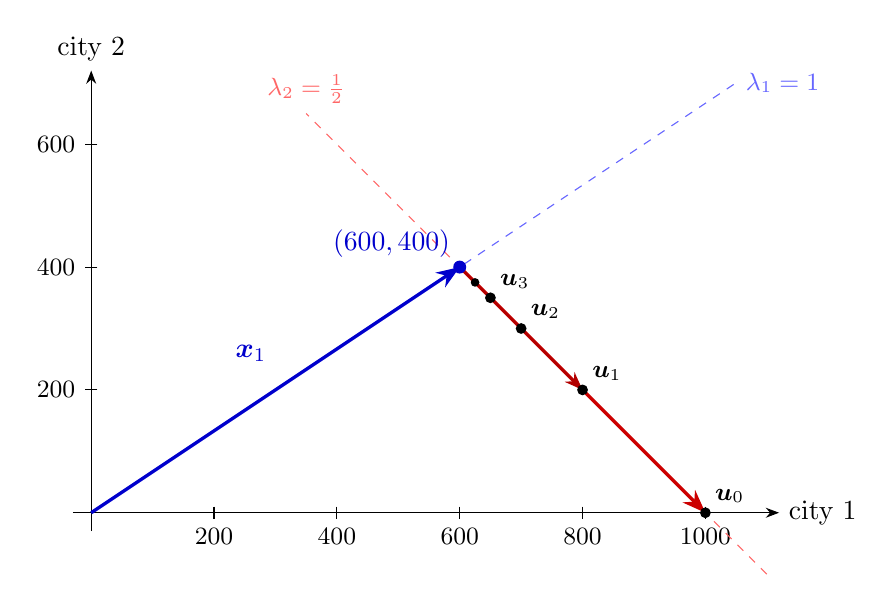
\begin{tikzpicture}[scale=0.78,>=Stealth]
  \draw[->] (-0.3,0) -- (11.2,0) node[right] {city 1};
  \draw[->] (0,-0.3) -- (0,7.2) node[above] {city 2};
  \foreach \x in {2,4,6,8,10} \draw (\x,0.1) -- (\x,-0.1) node[below] {\small $\x00$};
  \foreach \y in {2,4,6} \draw (0.1,\y) -- (-0.1,\y) node[left] {\small $\y00$};
  % eigenvector lines
  \draw[blue!60,dashed] (0,0) -- (10.5,7) node[right] {\small $\lambda_1=1$};
  \draw[red!60,dashed] (11,-1) -- (3.5,6.5) node[above] {\small $\lambda_2=\tfrac12$};
  % fixed arrow and sliding arrow
  \draw[->,very thick,blue!80!black] (0,0) -- (6,4);
  \draw[->,very thick,red!80!black] (6,4) -- (10,0);
  \draw[->,thick,red!70!black] (6,4) -- (8,2);
  % states
  \foreach \p/\l/\a in {(10,0)/0/above right,(8,2)/1/above right,(7,3)/2/above right,(6.5,3.5)/3/above right}
    \fill[black] \p circle (2.5pt) node[\a] {\small $\vb{u}_{\l}$};
  \fill[black] (6.25,3.75) circle (2pt);
  \fill[blue!80!black] (6,4) circle (3pt) node[above left] {$(600,400)$};
  \node[blue!80!black] at (2.6,2.6) {$\vb{x}_1$};
\end{tikzpicture}
\caption{The two-city model of Example~\ref{ex:u24-cities}. Every state lies on the line
$u_1+u_2=1000$ through the steady state $(600,400)$ in the direction $(1,-1)$. Each state is
the fixed arrow $(600,400)$ plus a sliding arrow $400(0.5)^{k}(1,-1)$; every year the sliding
arrow halves and the state hops $\vb{u}_0\to\vb{u}_1\to\vb{u}_2\to\dots$ toward $(600,400)$.}
\label{fig:u24-cities}
\end{figure}

\subsection{Fibonacci numbers}

The Fibonacci numbers $0,1,1,2,3,5,8,13,\dots$ obey $F_{k+2}=F_{k+1}+F_k$. How fast do
they grow, and what is $F_{100}$? The rule is a single second-order equation; a small trick
makes it a first-order system. Let $\vb{u}_k=(F_{k+1},F_k)$ and add the trivial equation
$F_{k+1}=F_{k+1}$:
\[
  \begin{aligned} F_{k+2}&=F_{k+1}+F_k\\ F_{k+1}&=F_{k+1}\end{aligned}
  \qquad\Longleftrightarrow\qquad
  \vb{u}_{k+1}=\begin{bmatrix} 1&1\\ 1&0\end{bmatrix}\vb{u}_k .
\]

\begin{example}[A formula for $F_k$]\label{ex:u24-fibonacci}
For $A=\left[\begin{smallmatrix} 1&1\\ 1&0\end{smallmatrix}\right]$ the trace is $1$ and the
determinant is $-1$, so
\[
  \det(A-\lambda I)=\lambda^{2}-\lambda-1=0,\qquad
  \lambda_1=\frac{1+\sqrt5}{2}\approx1.618,\qquad
  \lambda_2=\frac{1-\sqrt5}{2}\approx-0.618 .
\]
The equation $\lambda^{2}=\lambda+1$ is the Fibonacci rule itself. The eigenvalues are
distinct, so $A$ is diagonalizable. For the eigenvectors,
$A-\lambda I=\left[\begin{smallmatrix} 1-\lambda & 1\\ 1 & -\lambda\end{smallmatrix}\right]$
kills $(\lambda,1)$: the second row gives $\lambda-\lambda=0$ and the first gives
$(1-\lambda)\lambda+1=-(\lambda^{2}-\lambda-1)=0$. So $\vb{x}_1=(\lambda_1,1)$ and
$\vb{x}_2=(\lambda_2,1)$.

The start is $\vb{u}_0=(F_1,F_0)=(1,0)=c_1\vb{x}_1+c_2\vb{x}_2$. The second components give
$c_1+c_2=0$, the first $c_1\lambda_1+c_2\lambda_2=1$, so
$c_1=-c_2=1/(\lambda_1-\lambda_2)=1/\sqrt5$. Reading off the second component of
$\vb{u}_k=c_1\lambda_1^{k}\vb{x}_1+c_2\lambda_2^{k}\vb{x}_2$:
\[
  F_k=\frac{1}{\sqrt5}\left(\frac{1+\sqrt5}{2}\right)^{k}-\frac{1}{\sqrt5}\left(\frac{1-\sqrt5}{2}\right)^{k}.
\]
The second term is smaller than $\tfrac12$ in absolute value for every $k\ge0$ and shrinks
fast, so $F_k$ is the integer nearest to $\lambda_1^{k}/\sqrt5$. For $k=10$:
$\lambda_1^{10}/\sqrt5\approx55.004$ and $F_{10}=55$. For $k=100$: $F_{100}\approx3.54\times10^{20}$.
The large eigenvalue controls the growth: each Fibonacci number is about $1.618$ times the
previous one.
\end{example}

\subsection{Exercises}

\begin{exercise}\label{exr:u24-allX}
Describe all matrices $X$ that diagonalize
$A=\left[\begin{smallmatrix} 4&0\\ 1&2\end{smallmatrix}\right]$. Then describe all matrices
that diagonalize $A^{-1}$.
\end{exercise}
\begin{solution}
$A$ is triangular, so $\lambda_1=4$, $\lambda_2=2$. For $\lambda_1=4$:
$A-4I=\left[\begin{smallmatrix} 0&0\\ 1&-2\end{smallmatrix}\right]$, so $y=2z$ and the
eigenvectors are the nonzero multiples of $(2,1)$. For $\lambda_2=2$:
$A-2I=\left[\begin{smallmatrix} 2&0\\ 1&0\end{smallmatrix}\right]$, so $y=0$ and the
eigenvectors are the nonzero multiples of $(0,1)$. The diagonalizing matrices are
$X=\left[\begin{smallmatrix} 2a&0\\ a&b\end{smallmatrix}\right]$ and
$X=\left[\begin{smallmatrix} 0&2a\\ b&a\end{smallmatrix}\right]$ with $a,b\neq0$ (the
eigenvalues in $\Lambda$ then come in the order $4,2$ or $2,4$). Since
$A^{-1}=X\Lambda^{-1}X^{-1}$, exactly the same matrices diagonalize $A^{-1}$.
\end{solution}

\begin{exercise}\label{exr:u24-limit}
Diagonalize $A=\left[\begin{smallmatrix} 0.6&0.9\\ 0.4&0.1\end{smallmatrix}\right]$. What
is the limit of $\Lambda^{k}$ as $k\to\infty$? What is the limit of $X\Lambda^{k}X^{-1}$,
and what do you see in its columns?
\end{exercise}
\begin{solution}
Each column adds to $1$, so (as Section~\ref{sec:u26} explains) $\lambda_1=1$; the trace
$0.7$ gives $\lambda_2=-0.3$. From
$A-I=\left[\begin{smallmatrix} -0.4&0.9\\ 0.4&-0.9\end{smallmatrix}\right]$,
$\vb{x}_1=(9,4)$; from
$A+0.3I=\left[\begin{smallmatrix} 0.9&0.9\\ 0.4&0.4\end{smallmatrix}\right]$,
$\vb{x}_2=(1,-1)$. So
$X=\left[\begin{smallmatrix} 9&1\\ 4&-1\end{smallmatrix}\right]$,
$\Lambda=\operatorname{diag}(1,-0.3)$, and $\Lambda^{k}\to\operatorname{diag}(1,0)$ because
$|-0.3|<1$. With $X^{-1}=\tfrac1{13}\left[\begin{smallmatrix} 1&1\\ 4&-9\end{smallmatrix}\right]$,
\[
  A^{k}\to X\begin{bmatrix} 1&0\\ 0&0\end{bmatrix}X^{-1}
  =\begin{bmatrix} 9\\ 4\end{bmatrix}\frac{1}{13}\begin{bmatrix} 1&1\end{bmatrix}
  =\frac1{13}\begin{bmatrix} 9&9\\ 4&4\end{bmatrix}.
\]
Both columns are the steady state $(9,4)/13$: whatever the start (with components adding to
$1$), $A^{k}\vb{u}_0$ approaches it.
\end{solution}

\begin{exercise}\label{exr:u24-Ck}
For numbers $a\neq b$, let
$C=\left[\begin{smallmatrix} 2b-a & a-b\\ 2b-2a & 2a-b\end{smallmatrix}\right]$. Find the
eigenvalues and eigenvectors of $C$, a formula for $C^{k}$, and $C^{100}$ when $a=1$, $b=-1$.
\end{exercise}
\begin{solution}
The trace is $a+b$ and the determinant is $(2b-a)(2a-b)-(a-b)(2b-2a)=ab$, so
$\det(C-\lambda I)=\lambda^{2}-(a+b)\lambda+ab=(\lambda-a)(\lambda-b)$. For $\lambda=a$:
$C-aI=\left[\begin{smallmatrix} 2b-2a & a-b\\ 2b-2a & a-b\end{smallmatrix}\right]$; its first
column is $-2$ times its second, so $(1,2)$ is in the nullspace. For $\lambda=b$:
$C-bI=\left[\begin{smallmatrix} b-a & a-b\\ 2b-2a & 2a-2b\end{smallmatrix}\right]$, killed by
$(1,1)$. With $X=\left[\begin{smallmatrix} 1&1\\ 2&1\end{smallmatrix}\right]$ and
$X^{-1}=\left[\begin{smallmatrix} -1&1\\ 2&-1\end{smallmatrix}\right]$,
\[
  C^{k}=X\begin{bmatrix} a^{k}&0\\ 0&b^{k}\end{bmatrix}X^{-1}
  =\begin{bmatrix} 2b^{k}-a^{k} & a^{k}-b^{k}\\ 2b^{k}-2a^{k} & 2a^{k}-b^{k}\end{bmatrix}.
\]
At $k=1$ this is $C$, a useful check. For $a=1$, $b=-1$ and $k=100$, $a^{k}=b^{k}=1$ and
$C^{100}=\left[\begin{smallmatrix} 1&0\\ 0&1\end{smallmatrix}\right]=I$. (Here
$C=\left[\begin{smallmatrix} -3&2\\ -4&3\end{smallmatrix}\right]$ already has $C^{2}=I$.)
\end{solution}

\begin{exercise}\label{exr:u24-lucas}
The Lucas numbers $2,1,3,4,7,11,18,\dots$ follow the Fibonacci rule
$L_{k+2}=L_{k+1}+L_k$ but start from $L_0=2$, $L_1=1$. Show that
$L_k=\lambda_1^{k}+\lambda_2^{k}$ with $\lambda_{1,2}=(1\pm\sqrt5)/2$.
\end{exercise}
\begin{solution}
Use the same $A$ and eigenvectors as in Example~\ref{ex:u24-fibonacci} with
$\vb{u}_0=(L_1,L_0)=(1,2)$. The equations $c_1+c_2=2$ and $c_1\lambda_1+c_2\lambda_2=1$ are
solved by $c_1=c_2=1$, because $\lambda_1+\lambda_2=1$ (the trace). The second component of
$\vb{u}_k=\lambda_1^{k}\vb{x}_1+\lambda_2^{k}\vb{x}_2$ is $L_k=\lambda_1^{k}+\lambda_2^{k}$.
Check: $\lambda_1^{2}+\lambda_2^{2}=(\lambda_1+\lambda_2)^{2}-2\lambda_1\lambda_2=1+2=3=L_2$.
\end{solution}

\begin{exercise}\label{exr:u24-jordan}
Let $N=\left[\begin{smallmatrix} 1/2 & 1\\ 0 & 1/2\end{smallmatrix}\right]$. Show that $N$
is not diagonalizable, that
$N^{k}=\left[\begin{smallmatrix} 2^{-k} & k\,2^{1-k}\\ 0 & 2^{-k}\end{smallmatrix}\right]$,
and that $N^{k}\to0$ anyway.
\end{exercise}
\begin{solution}
The eigenvalue $\tfrac12$ is repeated, and $N-\tfrac12I=\left[\begin{smallmatrix} 0&1\\ 0&0\end{smallmatrix}\right]$
has only a one-dimensional nullspace, so there is just one independent eigenvector. The
formula holds for $k=1$; if it holds for $k$, then
\[
  N^{k+1}=N^{k}N=\begin{bmatrix} 2^{-k}\cdot\tfrac12 & 2^{-k}+k\,2^{1-k}\cdot\tfrac12\\ 0 & 2^{-k}\cdot\tfrac12\end{bmatrix}
  =\begin{bmatrix} 2^{-(k+1)} & (k+1)\,2^{-k}\\ 0 & 2^{-(k+1)}\end{bmatrix},
\]
which is the formula for $k+1$. Since $k\,2^{1-k}\to0$, $N^{k}\to0$. The off-diagonal entry
decays more slowly than $2^{-k}$ (it is $1,1,\tfrac34,\tfrac12,\dots$) because of the factor
$k$, but the decay of $|\lambda|^{k}$ wins in the end.
\end{solution}

% unit: u25
% sources: sources/066-differential-equations-and-exp-at.txt, sources/045-lecture-23-differential-equations-and-exp-at.txt, sources/200-mit18-06scf11-ses2-10sum-pdf-download-file.txt, sources/046-problem-solving-determinants-and-volumedifferential-equation.txt, sources/201-mit18-06scf11-ses2-10prob-pdf-download-file.txt, sources/202-mit18-06scf11-ses2-10sol-pdf-download-file.txt
\section{Differential equations and \texorpdfstring{\(e^{At}\)}{exp(At)}}\label{sec:u25}

Section~\ref{sec:u24} solved $\vb{u}_{k+1}=A\vb{u}_k$, where time moves in steps and the
solution is built from powers $\lambda^{k}$. Here time is continuous: we solve the system of
linear, constant-coefficient differential equations
\[
  \frac{d\vb{u}}{dt}=A\vb{u},\qquad \vb{u}(0)\ \text{given}.
\]
The key fact from calculus is that solutions of constant-coefficient linear equations are
exponentials. Looking for an exponential solution turns the differential equation into the
eigenvalue problem, and the whole section runs parallel to the previous one with
$e^{\lambda t}$ in place of $\lambda^{k}$.

\subsection{Pure exponential solutions}

Try $\vb{u}(t)=e^{\lambda t}\vb{x}$ with a fixed vector $\vb{x}$. Then
$d\vb{u}/dt=\lambda e^{\lambda t}\vb{x}$ while $A\vb{u}=e^{\lambda t}A\vb{x}$. These agree
for all $t$ exactly when $A\vb{x}=\lambda\vb{x}$. So every eigenvalue--eigenvector pair gives
a \emph{pure exponential solution} $e^{\lambda t}\vb{x}$, and since the equation is linear,
combinations of solutions are solutions.

\begin{theorem}[Solution by eigenvectors]\label{thm:u25-solution}
Let $A$ have $n$ independent eigenvectors $\vb{x}_1,\dots,\vb{x}_n$ with eigenvalues
$\lambda_1,\dots,\lambda_n$. Given $\vb{u}(0)$, solve $X\vb{c}=\vb{u}(0)$ for the coefficients
$c_i$. Then
\[
  \vb{u}(t)=c_1e^{\lambda_1t}\vb{x}_1+c_2e^{\lambda_2t}\vb{x}_2+\dots+c_ne^{\lambda_nt}\vb{x}_n
\]
solves $d\vb{u}/dt=A\vb{u}$ with the given initial value.
\end{theorem}

\begin{proof}
Each term satisfies the equation:
$\frac{d}{dt}\bigl(c_ie^{\lambda_it}\vb{x}_i\bigr)=c_i\lambda_ie^{\lambda_it}\vb{x}_i
=c_ie^{\lambda_it}A\vb{x}_i=A\bigl(c_ie^{\lambda_it}\vb{x}_i\bigr)$. Adding the terms, the sum
satisfies it too. At $t=0$ every exponential equals $1$, so
$\vb{u}(0)=c_1\vb{x}_1+\dots+c_n\vb{x}_n=X\vb{c}$, which is the given vector. (That this is
the \emph{only} solution follows from the matrix exponential below.)
\end{proof}

Set the two formulas side by side: $\vb{u}_k=\sum c_i\lambda_i^{k}\vb{x}_i$ for steps and
$\vb{u}(t)=\sum c_ie^{\lambda_it}\vb{x}_i$ for continuous time. Each eigenvector component
evolves on its own; $A$ couples the components of $\vb{u}$, and the eigenvectors uncouple
them.

\begin{example}[Flow between two compartments]\label{ex:u25-flow}
Solve
\[
  \frac{du_1}{dt}=-u_1+2u_2,\qquad \frac{du_2}{dt}=u_1-2u_2,\qquad \vb{u}(0)=(1,0).
\]
\emph{Eigenvalues.} $A=\left[\begin{smallmatrix} -1&2\\ 1&-2\end{smallmatrix}\right]$ is
singular (column~2 is $-2$ times column~1), so $\lambda_1=0$; the trace $-3$ gives
$\lambda_2=-3$. Directly, $\det(A-\lambda I)=\lambda^{2}+3\lambda=\lambda(\lambda+3)$.

\emph{Eigenvectors.} $A\vb{x}_1=\vb{0}$ gives $\vb{x}_1=(2,1)$.
$A+3I=\left[\begin{smallmatrix} 2&2\\ 1&1\end{smallmatrix}\right]$ gives $\vb{x}_2=(1,-1)$.

\emph{Coefficients.} $X\vb{c}=\vb{u}(0)$ reads $c_1(2,1)+c_2(1,-1)=(1,0)$; adding the
components, $3c_1=1$, and then $c_2=1-2c_1=\tfrac13$. So $c_1=c_2=\tfrac13$ and
\[
  \vb{u}(t)=\frac13\begin{bmatrix} 2\\ 1\end{bmatrix}+\frac13e^{-3t}\begin{bmatrix} 1\\ -1\end{bmatrix},
  \qquad\text{i.e.}\quad u_1=\tfrac23+\tfrac13e^{-3t},\quad u_2=\tfrac13-\tfrac13e^{-3t}.
\]
\emph{Check.} $u_1'=-e^{-3t}$ and $-u_1+2u_2=-\tfrac23-\tfrac13e^{-3t}+\tfrac23-\tfrac23e^{-3t}=-e^{-3t}$.

\emph{Interpretation.} Material flows out of compartment~1 into compartment~2. The
$e^{-3t}$ term dies out, and the $e^{0t}=1$ term stays: the solution approaches the steady
state $\vb{u}(\infty)=(\tfrac23,\tfrac13)$, the eigenvector for $\lambda=0$ scaled by $c_1$
(Figure~\ref{fig:u25-flow}). The total $u_1+u_2$ stays equal to $1$ throughout, because the
columns of $A$ add to zero, so $\frac{d}{dt}(u_1+u_2)=0$.
\end{example}

\begin{figure}[ht]\centering
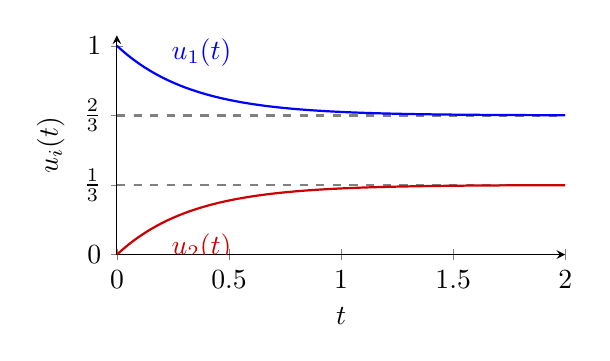
\begin{tikzpicture}
\begin{axis}[width=0.6\textwidth,height=0.36\textwidth,xmin=0,xmax=2,ymin=0,ymax=1.05,
  xlabel={$t$},ylabel={$u_i(t)$},axis lines=left,ytick={0,0.3333,0.6667,1},
  yticklabels={$0$,$\tfrac13$,$\tfrac23$,$1$},
  every axis plot/.append style={thick,samples=80}]
  \addplot[gray,dashed,domain=0:2] {2/3};
  \addplot[gray,dashed,domain=0:2] {1/3};
  \addplot[blue,domain=0:2] {2/3+exp(-3*x)/3} node[pos=0.12,above right] {$u_1(t)$};
  \addplot[red!80!black,domain=0:2] {1/3-exp(-3*x)/3} node[pos=0.12,below right] {$u_2(t)$};
\end{axis}
\end{tikzpicture}
\caption{The solution $u_1=\tfrac23+\tfrac13e^{-3t}$, $u_2=\tfrac13-\tfrac13e^{-3t}$ of
Example~\ref{ex:u25-flow}. The eigenvalue $\lambda_2=-3$ makes the
difference from the steady state decay like $e^{-3t}$ (by $t=1$ only $5\%$ of it is left);
the eigenvalue $\lambda_1=0$ supplies the steady state $(\tfrac23,\tfrac13)$.}
\label{fig:u25-flow}
\end{figure}

\subsection{Stability and steady states}

Which way the solution goes is decided by the eigenvalues alone. For a complex eigenvalue
$\lambda=a+ib$,
\[
  e^{\lambda t}=e^{at}e^{ibt}=e^{at}(\cos bt+i\sin bt),\qquad |e^{\lambda t}|=e^{at},
\]
since $\cos^{2}bt+\sin^{2}bt=1$. The imaginary part only makes the solution oscillate; the
real part decides growth or decay. For instance $\lambda=-3+6i$ gives $|e^{\lambda t}|=e^{-3t}$.
For a diagonalizable $A$, Theorem~\ref{thm:u25-solution} therefore gives three regimes:
\begin{enumerate}
  \item \emph{Stability}: $\vb{u}(t)\to\vb{0}$ for every start exactly when
  $\operatorname{Re}\lambda_i<0$ for every $i$.
  \item \emph{Steady state}: if $\lambda_1=0$ and all other $\operatorname{Re}\lambda_i<0$,
  then $\vb{u}(t)\to c_1\vb{x}_1$.
  \item \emph{Blow-up}: if some $\operatorname{Re}\lambda_i>0$, every start with $c_i\neq0$
  produces a solution that grows without bound.
\end{enumerate}
Changing $A$ to $-A$ changes the sign of every eigenvalue: in Example~\ref{ex:u25-flow} it
would turn $e^{-3t}$ into $e^{3t}$ and the steady state into blow-up.

\begin{figure}[ht]\centering
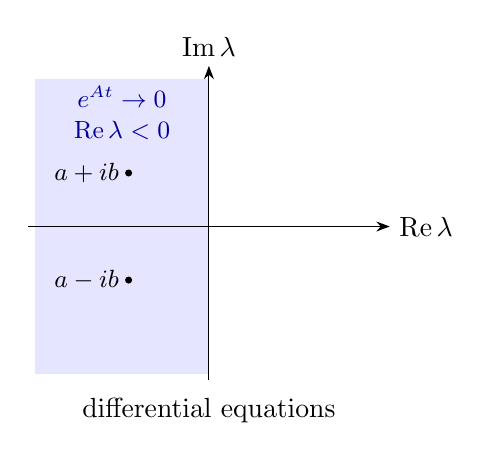
\begin{tikzpicture}[scale=0.85,>=Stealth]
  \fill[blue!10] (-2.6,-2.2) rectangle (0,2.2);
  \draw[->] (-2.7,0) -- (2.7,0) node[right] {$\operatorname{Re}\lambda$};
  \draw[->] (0,-2.3) -- (0,2.4) node[above] {$\operatorname{Im}\lambda$};
  \node[blue!60!black,align=center] at (-1.3,1.7) {\small $e^{At}\to0$\\[-1pt]\small $\operatorname{Re}\lambda<0$};
  \fill (-1.2,0.8) circle (1.5pt); \fill (-1.2,-0.8) circle (1.5pt);
  \node[left] at (-1.2,-0.8) {\small $a-ib$}; \node[left] at (-1.2,0.8) {\small $a+ib$};
  \node at (0,-2.75) {differential equations};
\end{tikzpicture}\qquad
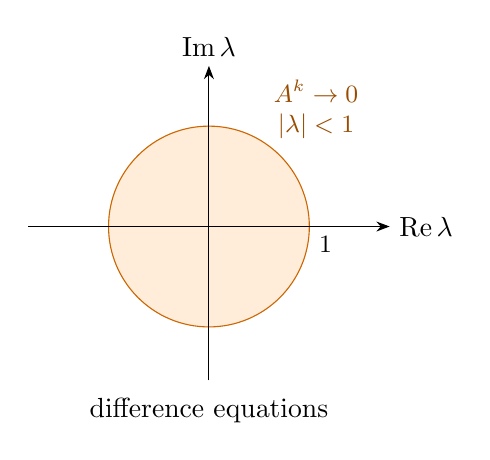
\begin{tikzpicture}[scale=0.85,>=Stealth]
  \fill[orange!15] (0,0) circle (1.5);
  \draw[orange!80!black] (0,0) circle (1.5);
  \draw[->] (-2.7,0) -- (2.7,0) node[right] {$\operatorname{Re}\lambda$};
  \draw[->] (0,-2.3) -- (0,2.4) node[above] {$\operatorname{Im}\lambda$};
  \node[orange!60!black,align=center] at (1.6,1.75) {\small $A^{k}\to0$\\[-1pt]\small $|\lambda|<1$};
  \node[below right] at (1.5,0) {\small $1$};
  \node at (0,-2.75) {difference equations};
\end{tikzpicture}
\caption{Where the eigenvalues must lie for the solutions to decay. For
$d\vb{u}/dt=A\vb{u}$ it is the left half-plane $\operatorname{Re}\lambda<0$; for
$\vb{u}_{k+1}=A\vb{u}_k$ it is the inside of the unit circle $|\lambda|<1$. The eigenvalue
$\lambda=0$ gives a steady state for differential equations; $\lambda=1$ gives one for powers.}
\label{fig:u25-regions}
\end{figure}

For $2\times2$ matrices there is a test that needs no eigenvalues at all.

\begin{proposition}[Stability of a $2\times2$ system]\label{prop:u25-2by2}
A real $2\times2$ matrix $A$ has both eigenvalues with negative real part if and only if
\[
  \tr A<0\qquad\text{and}\qquad\det A>0 .
\]
\end{proposition}

\begin{proof}
Recall $\tr A=\lambda_1+\lambda_2$ and $\det A=\lambda_1\lambda_2$
(Section~\ref{sec:u23}). If the eigenvalues are a complex pair $a\pm ib$ ($b\neq0$),
then $\tr A=2a$ and $\det A=a^{2}+b^{2}>0$, so the condition says exactly $a<0$. If they are
real, $\det A>0$ means they have the same sign and $\tr A<0$ means that sign is negative;
conversely two negative numbers have negative sum and positive product.
\end{proof}

A negative trace alone is not enough: $\left[\begin{smallmatrix} -2&0\\ 0&1\end{smallmatrix}\right]$
has trace $-1$ but eigenvalues $-2$ and $1$, so $e^{t}$ blows up. Its determinant $-2$ fails
the test.

\subsection{The matrix exponential}

For a single equation $du/dt=au$ the solution is $u(t)=e^{at}u(0)$. We would like to write
$\vb{u}(t)=e^{At}\vb{u}(0)$ for systems. The exponential of a matrix is defined by the same
power series as $e^{x}$.

\begin{definition}[Matrix exponential]\label{def:u25-exp}
For a square matrix $A$ and a number $t$,
\[
  e^{At}=I+At+\frac{(At)^{2}}{2!}+\frac{(At)^{3}}{3!}+\dots=\sum_{k=0}^{\infty}\frac{(At)^{k}}{k!}.
\]
\end{definition}

The series always converges: if every entry of $A$ has absolute value at most $m$, every entry
of $A^{k}$ has absolute value at most $(nm)^{k}$, and $\sum (nm|t|)^{k}/k!$ is finite. Compare
the geometric series $(I-At)^{-1}=I+At+(At)^{2}+\cdots$, which has no factorials and converges
only when the eigenvalues of $At$ are smaller than $1$ in absolute value; for small $t$ it says
$(I-At)^{-1}\approx I+At$.

\begin{proposition}[The exponential solves the system]\label{prop:u25-derivative}
$\dfrac{d}{dt}e^{At}=Ae^{At}$ and $e^{A\cdot0}=I$. Hence $\vb{u}(t)=e^{At}\vb{u}(0)$ solves
$d\vb{u}/dt=A\vb{u}$ with the given $\vb{u}(0)$.
\end{proposition}

\begin{proof}
Differentiate the series term by term (allowed for power series):
$\frac{d}{dt}\frac{t^{k}A^{k}}{k!}=\frac{t^{k-1}A^{k}}{(k-1)!}=A\,\frac{(At)^{k-1}}{(k-1)!}$.
Summing over $k\ge1$ gives $A\,e^{At}$. At $t=0$ only the term $I$ survives.
\end{proof}

The formula needs no eigenvectors, so it also covers matrices that are not diagonalizable.
It also gives uniqueness: if $\vb{u}$ is any solution, then
$\frac{d}{dt}\bigl(e^{-At}\vb{u}\bigr)=-Ae^{-At}\vb{u}+e^{-At}A\vb{u}=\vb{0}$ (the series show that
$A$ commutes with $e^{-At}$), so $e^{-At}\vb{u}(t)$ is constant, equal to $\vb{u}(0)$. And
$e^{At}e^{-At}=I$, because this product has derivative $Ae^{At}e^{-At}-e^{At}Ae^{-At}=0$ and
equals $I$ at $t=0$; multiplying by $e^{At}$ gives $\vb{u}(t)=e^{At}\vb{u}(0)$. When $A$ \emph{is} diagonalizable, the
eigenvectors make the series easy to sum.

\begin{theorem}[Exponential by diagonalization]\label{thm:u25-diagexp}
If $A=X\Lambda X^{-1}$, then
\[
  e^{At}=Xe^{\Lambda t}X^{-1},\qquad
  e^{\Lambda t}=\begin{bmatrix} e^{\lambda_1t} & & \\ & \ddots & \\ & & e^{\lambda_nt}\end{bmatrix}.
\]
\end{theorem}

\begin{proof}
As in Section~\ref{sec:u24}, $(At)^{k}=X\Lambda^{k}X^{-1}t^{k}$. Write $I=XX^{-1}$ and
factor $X$ out on the left and $X^{-1}$ on the right of every term:
\[
  e^{At}=X\Bigl(I+\Lambda t+\frac{(\Lambda t)^{2}}{2!}+\cdots\Bigr)X^{-1}=Xe^{\Lambda t}X^{-1}.
\]
The series for the diagonal matrix $\Lambda t$ is diagonal, with the scalar series
$\sum(\lambda_it)^{k}/k!=e^{\lambda_it}$ on the diagonal.
\end{proof}

Another way to see the same thing: substitute $\vb{u}=X\vb{v}$. Then $X\,d\vb{v}/dt=AX\vb{v}$,
so $d\vb{v}/dt=X^{-1}AX\vb{v}=\Lambda\vb{v}$, which is $n$ separate scalar equations
$dv_i/dt=\lambda_iv_i$ with solutions $v_i(t)=e^{\lambda_it}v_i(0)$. Going back,
$\vb{u}(t)=Xe^{\Lambda t}X^{-1}\vb{u}(0)$, and with $\vb{c}=X^{-1}\vb{u}(0)$ this is the sum
in Theorem~\ref{thm:u25-solution}. It also shows again that $e^{At}\to0$ exactly when every
$e^{\lambda_it}\to0$, that is, every $\operatorname{Re}\lambda_i<0$.

\begin{example}[Computing $e^{At}$]\label{ex:u25-exp}
Let $A=\begin{bmatrix} 1&1\\ 0&3\end{bmatrix}$. It is triangular: $\lambda_1=1$ with
$\vb{x}_1=(1,0)$, and $\lambda_2=3$ with $\vb{x}_2=(1,2)$ from
$A-3I=\left[\begin{smallmatrix} -2&1\\ 0&0\end{smallmatrix}\right]$. So
\[
  X=\begin{bmatrix} 1&1\\ 0&2\end{bmatrix},\qquad
  X^{-1}=\begin{bmatrix} 1&-\tfrac12\\ 0&\tfrac12\end{bmatrix},\qquad
  e^{At}=\begin{bmatrix} 1&1\\ 0&2\end{bmatrix}
  \begin{bmatrix} e^{t}&0\\ 0&e^{3t}\end{bmatrix}
  \begin{bmatrix} 1&-\tfrac12\\ 0&\tfrac12\end{bmatrix}
  =\begin{bmatrix} e^{t} & \tfrac12(e^{3t}-e^{t})\\ 0 & e^{3t}\end{bmatrix}.
\]
Check: at $t=0$ this is $I$. Its derivative is
$\left[\begin{smallmatrix} e^{t} & \frac12(3e^{3t}-e^{t})\\ 0 & 3e^{3t}\end{smallmatrix}\right]$,
which at $t=0$ equals $\left[\begin{smallmatrix} 1&1\\ 0&3\end{smallmatrix}\right]=A$, as
Proposition~\ref{prop:u25-derivative} requires.
\end{example}

\begin{trap}
The exponential of a matrix is \emph{not} the matrix of exponentials of its entries. In
Example~\ref{ex:u25-exp} the $(1,2)$ entry of $e^{At}$ is $\tfrac12(e^{3t}-e^{t})$, not
$e^{t}$, and the zero entry gives $0$, not $e^{0}=1$. Similarly $e^{A}e^{B}=e^{A+B}$ is true
when $AB=BA$ but false in general. When $A$ cannot be diagonalized, new kinds of terms
appear: for $A=\left[\begin{smallmatrix} 0&1\\ 0&0\end{smallmatrix}\right]$ we have $A^{2}=0$,
the series stops, and $e^{At}=I+At=\left[\begin{smallmatrix} 1&t\\ 0&1\end{smallmatrix}\right]$
contains $t\,e^{0t}$, which is not a pure exponential.
\end{trap}

\subsection{Higher-order equations become first-order systems}

The second-order equation $y''+by'+ky=0$ becomes a $2\times2$ system by the same trick as
for Fibonacci: take $\vb{u}=(y',y)$ and add the trivial equation $y'=y'$,
\[
  \vb{u}'=\begin{bmatrix} y''\\ y'\end{bmatrix}
  =\begin{bmatrix} -b&-k\\ 1&0\end{bmatrix}\begin{bmatrix} y'\\ y\end{bmatrix}.
\]
Its characteristic polynomial is
$\det\left[\begin{smallmatrix} -b-\lambda & -k\\ 1 & -\lambda\end{smallmatrix}\right]
=\lambda^{2}+b\lambda+k$, exactly what we get by substituting $y=e^{\lambda t}$ into the
original equation. An equation of order $m$ gives an $m\times m$ matrix with the
coefficients (with signs changed) across the first row, $1$'s just below the diagonal, and
zeros elsewhere. For such a matrix the vector $(\lambda^{m-1},\dots,\lambda,1)$ is an
eigenvector whenever $\lambda$ is an eigenvalue: the rows below the first just say
$\lambda^{j}=\lambda\cdot\lambda^{j-1}$, and the first row is the characteristic equation.

\begin{example}[A third-order equation]\label{ex:u25-third}
Solve $y'''+2y''-y'-2y=0$ and find the first column of $e^{At}$ for the corresponding
system.

With $\vb{u}=(y'',y',y)$, the equation $y'''=-2y''+y'+2y$ gives
\[
  \vb{u}'=A\vb{u},\qquad A=\begin{bmatrix} -2&1&2\\ 1&0&0\\ 0&1&0\end{bmatrix}.
\]
Expanding along the first row,
\[
  \det(A-\lambda I)=(-2-\lambda)\lambda^{2}-1\cdot(-\lambda)+2\cdot1
  =-(\lambda^{3}+2\lambda^{2}-\lambda-2)=-(\lambda-1)(\lambda+1)(\lambda+2),
\]
so $\lambda=1,-1,-2$, with eigenvectors $(\lambda^{2},\lambda,1)$:
$\vb{x}_1=(1,1,1)$, $\vb{x}_2=(1,-1,1)$, $\vb{x}_3=(4,-2,1)$. The last component of
$\vb{u}(t)=C_1e^{t}\vb{x}_1+C_2e^{-t}\vb{x}_2+C_3e^{-2t}\vb{x}_3$ is
\[
  y(t)=C_1e^{t}+C_2e^{-t}+C_3e^{-2t}.
\]
Because $\lambda=1>0$, solutions blow up unless $C_1=0$.

To get the first column of $e^{At}=Xe^{\Lambda t}X^{-1}$, only the first column of
$X^{-1}$ is needed. By the cofactor formula of Section~\ref{sec:u22} ($X^{-1}$ is the transposed cofactor matrix divided by $\det X$), that column is the cofactors of the
first row of $X$ divided by $\det X$. For
$X=\left[\begin{smallmatrix} 1&1&4\\ 1&-1&-2\\ 1&1&1\end{smallmatrix}\right]$ the cofactors
of the first row are
\[
  C_{11}=(-1)(1)-(-2)(1)=1,\qquad C_{12}=-\bigl(1\cdot1-(-2)\cdot1\bigr)=-3,\qquad
  C_{13}=1\cdot1-(-1)\cdot1=2,
\]
and $\det X=1\cdot1+1\cdot(-3)+4\cdot2=6$. So the first column of $X^{-1}$ is
$(\tfrac16,-\tfrac12,\tfrac13)$, and the first column of $e^{At}$ is
\[
  \tfrac16e^{t}\,\vb{x}_1-\tfrac12e^{-t}\,\vb{x}_2+\tfrac13e^{-2t}\,\vb{x}_3 .
\]
At $t=0$ it equals $\tfrac16(1,1,1)-\tfrac12(1,-1,1)+\tfrac13(4,-2,1)=(1,0,0)$, the first
column of $I$, as it must.
\end{example}

\subsection{Exercises}

\begin{exercise}[Skew-symmetric systems conserve length]\label{exr:u25-skew}
The matrix in
\[
  \frac{d\vb{u}}{dt}=\begin{bmatrix} 0&c&-b\\ -c&0&a\\ b&-a&0\end{bmatrix}\vb{u},
  \quad\text{that is,}\quad u_1'=cu_2-bu_3,\ \ u_2'=au_3-cu_1,\ \ u_3'=bu_1-au_2,
\]
is skew-symmetric ($A\T=-A$). Compute
$\frac{d}{dt}\|\vb{u}(t)\|^{2}$. What does this say about $\vb{u}(t)$?
\end{exercise}
\begin{solution}
\[
  \frac{d}{dt}(u_1^{2}+u_2^{2}+u_3^{2})=2u_1u_1'+2u_2u_2'+2u_3u_3'
  =2u_1(cu_2-bu_3)+2u_2(au_3-cu_1)+2u_3(bu_1-au_2)=0,
\]
since the six products cancel in pairs. So $\|\vb{u}(t)\|=\|\vb{u}(0)\|$ for all $t$: the
solution stays on the sphere of radius $\|\vb{u}(0)\|$, neither decaying nor blowing up. In
matrix form, $\frac{d}{dt}\vb{u}\T\vb{u}=\vb{u}\T(A\T+A)\vb{u}=0$ because $A\T=-A$.
Consistently, the eigenvalues of a real skew-symmetric matrix are purely imaginary
(Section~\ref{sec:u23}).
\end{solution}

\begin{exercise}[The exponential of a rotation generator]\label{exr:u25-rotation}
For $A=\left[\begin{smallmatrix} 0&-1\\ 1&0\end{smallmatrix}\right]$ show that
$e^{At}=\left[\begin{smallmatrix} \cos t & -\sin t\\ \sin t & \cos t\end{smallmatrix}\right]$.
Describe the solutions of $d\vb{u}/dt=A\vb{u}$.
\end{exercise}
\begin{solution}
$A^{2}=-I$, so $A^{3}=-A$, $A^{4}=I$, and the powers repeat with period $4$. Group the series:
\[
  e^{At}=\Bigl(1-\frac{t^{2}}{2!}+\frac{t^{4}}{4!}-\cdots\Bigr)I+\Bigl(t-\frac{t^{3}}{3!}+\cdots\Bigr)A
  =(\cos t)\,I+(\sin t)\,A,
\]
which is the stated rotation matrix. (Equivalently, the eigenvalues are $\pm i$ and
$e^{\pm it}=\cos t\pm i\sin t$.) Every solution $\vb{u}(t)=e^{At}\vb{u}(0)$ rotates
$\vb{u}(0)$ through the angle $t$: it circles the origin at constant length, the case
$\operatorname{Re}\lambda=0$ between decay and blow-up.
\end{solution}

\begin{exercise}[Stability by trace and determinant]\label{exr:u25-classify}
Decide whether solutions of $d\vb{u}/dt=A\vb{u}$ decay, blow up, or neither, for
\[
  \text{(a)}\ \begin{bmatrix} -1&5\\ -1&-1\end{bmatrix},\quad
  \text{(b)}\ \begin{bmatrix} -3&1\\ 1&-3\end{bmatrix},\quad
  \text{(c)}\ \begin{bmatrix} 0&1\\ -4&0\end{bmatrix},\quad
  \text{(d)}\ \begin{bmatrix} 1&2\\ 3&4\end{bmatrix}.
\]
\end{exercise}
\begin{solution}
Use Proposition~\ref{prop:u25-2by2}.
(a) $\tr=-2<0$, $\det=1+5=6>0$: stable. The eigenvalues are $-1\pm i\sqrt5$, so solutions
spiral into the origin.
(b) $\tr=-6$, $\det=9-1=8$: stable, with real eigenvalues $-2$ and $-4$.
(c) $\tr=0$, $\det=4$: the eigenvalues are $\pm2i$, with real part $0$. Solutions oscillate
like $\cos2t$ and $\sin2t$ forever, neither decaying nor growing. (This is $y''+4y=0$
written as a system for $(y,y')$.)
(d) $\tr=5$, $\det=4-6=-2<0$: one positive and one negative eigenvalue,
$\tfrac12(5\pm\sqrt{33})$, so solutions blow up except along one eigenvector line.
\end{solution}

\begin{exercise}[A damped oscillator]\label{exr:u25-damped}
Solve $y''+3y'+2y=0$ with $y(0)=1$, $y'(0)=0$ by writing it as a system for
$\vb{u}=(y',y)$.
\end{exercise}
\begin{solution}
$A=\left[\begin{smallmatrix} -3&-2\\ 1&0\end{smallmatrix}\right]$ and
$\det(A-\lambda I)=\lambda^{2}+3\lambda+2=(\lambda+1)(\lambda+2)$. The eigenvectors are
$(\lambda,1)$: $\vb{x}_1=(-1,1)$ for $\lambda=-1$ and $\vb{x}_2=(-2,1)$ for $\lambda=-2$.
The start $\vb{u}(0)=(y'(0),y(0))=(0,1)=c_1(-1,1)+c_2(-2,1)$ gives $-c_1-2c_2=0$ and
$c_1+c_2=1$, so $c_2=-1$, $c_1=2$. The second component of
$\vb{u}(t)=2e^{-t}\vb{x}_1-e^{-2t}\vb{x}_2$ is
\[
  y(t)=2e^{-t}-e^{-2t}.
\]
Check: $y(0)=1$, $y'(t)=-2e^{-t}+2e^{-2t}$ so $y'(0)=0$, and
$y''+3y'+2y=(2e^{-t}-4e^{-2t})+(-6e^{-t}+6e^{-2t})+(4e^{-t}-2e^{-2t})=0$. Both eigenvalues
are negative (trace $-3$, determinant $2$), so $y\to0$ without oscillating.
\end{solution}

% unit: u26
% sources: sources/085-markov-matrices-fourier-series.txt, sources/047-lecture-24-markov-matrices-fourier-series.txt, sources/203-mit18-06scf11-ses2-11sum-pdf-download-file.txt, sources/048-problem-solving-markov-matrices.txt, sources/204-mit18-06scf11-ses2-11prob-pdf-download-file.txt, sources/205-mit18-06scf11-ses2-11sol-pdf-download-file.txt, short_plan.json (s04)
\section{Markov matrices; Fourier series}\label{sec:u26}

This section gives two applications. The first uses eigenvalues: a Markov matrix moves
probabilities or populations around without creating or destroying any, and its powers
approach a steady state given by the eigenvector for $\lambda=1$. The second uses
projections: expanding a vector in an orthonormal basis is easy, and Fourier series are
exactly that expansion carried out in a space of functions.

\subsection{\texorpdfstring{\(A\)}{A} and \texorpdfstring{\(A\T\)}{its transpose} have the same eigenvalues}

\begin{proposition}[Eigenvalues of the transpose]\label{prop:u26-transpose}
For every square matrix $A$, $\det(A\T-\lambda I)=\det(A-\lambda I)$. So $A\T$ has the same
eigenvalues as $A$, with the same multiplicities.
\end{proposition}

\begin{proof}
$(A-\lambda I)\T=A\T-\lambda I$, because $I\T=I$; and a matrix and its transpose have the
same determinant (property~10, Section~\ref{sec:u20}).
\end{proof}

The eigen\emph{vectors} are usually different: an eigenvector of $A\T$ for $\lambda$ lies in
$\Nul{A\T-\lambda I}$, the left nullspace of $A-\lambda I$, not in its nullspace.

\subsection{Markov matrices}

\begin{definition}[Markov matrix]\label{def:u26-markov}
A square matrix is a \emph{Markov matrix} if every entry is nonnegative and every column
adds to $1$. With $\vb{1}=(1,1,\dots,1)$, the column condition reads $\vb{1}\T A=\vb{1}\T$.
\end{definition}

The two conditions come from probability. Entry $a_{ij}$ is the probability (or fraction of
the population) that moves from state $j$ to state $i$ in one step; probabilities are never
negative, and everything in state $j$ must go somewhere, so column $j$ adds to $1$. A
typical example is
\[
  A=\begin{bmatrix} 0.1&0.01&0.3\\ 0.2&0.99&0.3\\ 0.7&0&0.4\end{bmatrix}.
\]
Powers of a Markov matrix are Markov matrices: products of nonnegative matrices are
nonnegative, and $\vb{1}\T A^{2}=(\vb{1}\T A)A=\vb{1}\T A=\vb{1}\T$. The same computation
shows that the step $\vb{u}_{k+1}=A\vb{u}_k$ conserves the total:
$\vb{1}\T\vb{u}_{k+1}=\vb{1}\T A\vb{u}_k=\vb{1}\T\vb{u}_k$.

\begin{theorem}[Eigenvalues of a Markov matrix]\label{thm:u26-markov}
Let $A$ be a Markov matrix. Then $\lambda=1$ is an eigenvalue of $A$, and every eigenvalue
satisfies $|\lambda|\le1$.
\end{theorem}

\begin{proof}
\emph{$\lambda=1$.} Every column of $A-I$ adds to $0$, so adding all the rows of $A-I$ gives
the zero row: $\vb{1}\T(A-I)=\vb{0}\T$. The rows are dependent, so $A-I$ is singular and $1$
is an eigenvalue. (Equivalently, $A\T\vb{1}=\vb{1}$, so $\vb{1}$ is an eigenvector of $A\T$,
and Proposition~\ref{prop:u26-transpose} transfers the eigenvalue to $A$.)

\emph{$|\lambda|\le1$.} By Proposition~\ref{prop:u26-transpose} it suffices to treat $A\T$.
Let $A\T\vb{y}=\lambda\vb{y}$ with $\vb{y}\neq\vb{0}$, and choose $i$ with $|y_i|$ as large as
possible. Row $i$ of $A\T$ is column $i$ of $A$, so
\[
  |\lambda|\,|y_i|=\Bigl|\sum_j a_{ji}\,y_j\Bigr|\le\sum_j a_{ji}\,|y_j|\le|y_i|\sum_j a_{ji}=|y_i|,
\]
using $a_{ji}\ge0$ and the column sum $1$. Divide by $|y_i|>0$.
\end{proof}

The eigenvector for $\lambda=1$ is the interesting one. It is found in the nullspace of $A-I$
(not from $\vb{1}$, which lies in the left nullspace). Two more facts, which we state without
proof (they are part of the Perron--Frobenius theorem): this eigenvector can be chosen with
no negative components, and if every entry of $A$ is positive then every other eigenvalue has
$|\lambda|<1$. Zero entries can allow other eigenvalues on the unit circle: the permutation
$\left[\begin{smallmatrix} 0&1\\ 1&0\end{smallmatrix}\right]$ is a Markov matrix with
$\lambda=-1$, and its powers swap two states forever without settling down.

\begin{example}[Finding the steady-state eigenvector]\label{ex:u26-3by3}
For the $3\times3$ matrix above,
\[
  A-I=\begin{bmatrix} -0.9&0.01&0.3\\ 0.2&-0.01&0.3\\ 0.7&0&-0.6\end{bmatrix}.
\]
The last row says $0.7x_1=0.6x_3$, so try $x_1=0.6$, $x_3=0.7$. The first row then requires
$-0.54+0.01x_2+0.21=0$, so $x_2=33$. Check the middle row:
$0.12-0.33+0.21=0$. So $\vb{x}_1=(0.6,\,33,\,0.7)$, with all components positive as
promised. The middle state, which keeps $99\%$ of its contents each step, ends up holding
almost everything.
\end{example}

Now combine Theorem~\ref{thm:u26-markov} with the solution of difference equations
(Section~\ref{sec:u24}). If $A$ has independent eigenvectors, $\lambda_1=1$,
and $|\lambda_i|<1$ for $i\ge2$, then
\[
  \vb{u}_k=c_1\,1^{k}\,\vb{x}_1+c_2\lambda_2^{k}\vb{x}_2+\dots+c_n\lambda_n^{k}\vb{x}_n
  \;\longrightarrow\;c_1\vb{x}_1 .
\]
The limit is the steady state: the $\vb{x}_1$-component of the start. Because the total is
conserved, the multiple $c_1$ is fixed by $\vb{1}\T(c_1\vb{x}_1)=\vb{1}\T\vb{u}_0$. Steady states
come from $\lambda=0$ for differential equations (Section~\ref{sec:u25}) but from
$\lambda=1$ for powers.

\begin{figure}[ht]\centering
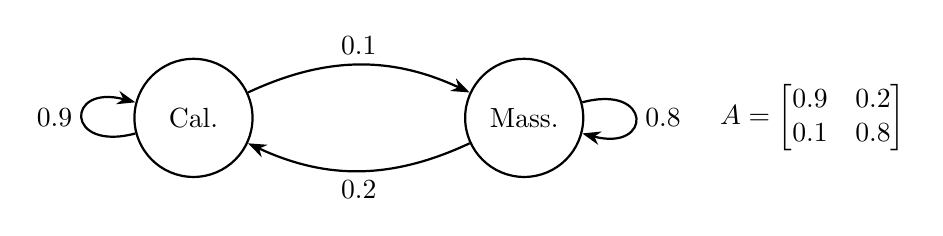
\begin{tikzpicture}[>=Stealth,node distance=4.2cm,
  st/.style={circle,draw,thick,minimum size=1.5cm,align=center}]
  \node[st] (C) {Cal.};
  \node[st,right of=C] (M) {Mass.};
  \draw[->,thick] (C) to[bend left=25] node[above] {$0.1$} (M);
  \draw[->,thick] (M) to[bend left=25] node[below] {$0.2$} (C);
  \draw[->,thick] (C) to[loop left,looseness=6] node[left] {$0.9$} (C);
  \draw[->,thick] (M) to[loop right,looseness=6] node[right] {$0.8$} (M);
  \node[right=1.6cm of M] {$A=\begin{bmatrix} 0.9&0.2\\ 0.1&0.8\end{bmatrix}$};
\end{tikzpicture}
\caption{A two-state Markov chain and its matrix. Column $j$ of $A$ lists where the
population of state $j$ goes in one year: the arrows leaving California carry $0.9$ and
$0.1$, which form column~1 and add to $1$.}
\label{fig:u26-chain}
\end{figure}

\begin{example}[California and Massachusetts]\label{ex:u26-calmass}
Each year $90\%$ of the people in California stay and $10\%$ move to Massachusetts, while
$80\%$ of Massachusetts stays and $20\%$ moves to California (Figure~\ref{fig:u26-chain}).
Start with everyone in Massachusetts:
$\vb{u}_0=(u_{\text{Cal}},u_{\text{Mass}})=(0,1000)$.

After one year $\vb{u}_1=A\vb{u}_0=1000\,(0.2,0.8)=(200,800)$. For the long run we need the
eigenvalues: $\lambda_1=1$ (Markov), and the trace $1.7$ gives $\lambda_2=0.7$ (check:
$\det A=0.72-0.02=0.7$). The eigenvectors come from
\[
  A-I=\begin{bmatrix} -0.1&0.2\\ 0.1&-0.2\end{bmatrix}\Rightarrow\vb{x}_1=(2,1),\qquad
  A-0.7I=\begin{bmatrix} 0.2&0.2\\ 0.1&0.1\end{bmatrix}\Rightarrow\vb{x}_2=(-1,1).
\]
Matching the start, $c_1(2,1)+c_2(-1,1)=(0,1000)$ gives $c_1=\tfrac{1000}{3}$ and
$c_2=\tfrac{2000}{3}$. Hence
\[
  \vb{u}_k=\frac{1000}{3}\begin{bmatrix} 2\\ 1\end{bmatrix}
  +\frac{2000}{3}(0.7)^{k}\begin{bmatrix} -1\\ 1\end{bmatrix}.
\]
At $k=1$ this gives $(\tfrac{2000-1400}{3},\tfrac{1000+1400}{3})=(200,800)$, as computed
directly; then $(340,660)$ and $(438,562)$. The populations approach
$(666\tfrac23,\,333\tfrac13)$: two thirds in California, from any start with $1000$ people.
The gap shrinks by the factor $0.7$ each year.
\end{example}

\begin{example}[The two-city model as a Markov chain]\label{ex:u26-twocity}
The matrix $A=\left[\begin{smallmatrix} 0.8&0.3\\ 0.2&0.7\end{smallmatrix}\right]$ of
the two-city example of Section~\ref{sec:u24} is a Markov matrix, which is why $\lambda_1=1$ appeared there;
$\lambda_2=1.5-1=0.5$ came from the trace. Its powers approach
\[
  A^{k}\to\begin{bmatrix} 0.6&0.6\\ 0.4&0.4\end{bmatrix}
  =\begin{bmatrix} 0.6\\ 0.4\end{bmatrix}\begin{bmatrix} 1&1\end{bmatrix},
\]
a matrix whose columns are both the steady state $(0.6,0.4)$. So
$A^{k}\vb{u}_0\to(0.6,0.4)\,(u_1+u_2)$ for every start: the long-run split does not depend on
where the 1000 people begin. Starting from $(0,1000)=(600,400)-600(1,-1)$, the first year
gives $A(0,1000)=(300,700)$, and
$\vb{u}_k=(600,400)-600(0.5)^{k}(1,-1)$ settles at $(600,400)$, the same limit as from
$(1000,0)$. Only the size of the decaying $\lambda=0.5$ part depends on the start.
\end{example}

\begin{remark}[Rows instead of columns]
Many probability texts multiply a row vector by the matrix from the left, $\vb{p}_{k+1}\T=\vb{p}_k\T P$.
Then $P=A\T$ and it is the \emph{rows} that add to $1$. Everything above holds after
transposing.
\end{remark}

\subsection{Expansion in an orthonormal basis}

Let $\vb{q}_1,\dots,\vb{q}_n$ be an orthonormal basis of $\R^{n}$. Every $\vb{v}$ is a
combination $\vb{v}=x_1\vb{q}_1+\dots+x_n\vb{q}_n$, and orthonormality makes the coefficients
trivial to find.

\begin{proposition}[Coefficients in an orthonormal basis]\label{prop:u26-coeff}
If $\vb{v}=x_1\vb{q}_1+\dots+x_n\vb{q}_n$ with orthonormal $\vb{q}_i$, then
$x_i=\vb{q}_i\T\vb{v}$. In matrix form, $Q\vb{x}=\vb{v}$ gives $\vb{x}=Q\T\vb{v}$.
\end{proposition}

\begin{proof}
Take the dot product of both sides with $\vb{q}_i$. Since $\vb{q}_i\T\vb{q}_j=0$ for $j\neq i$
and $\vb{q}_i\T\vb{q}_i=1$, every term on the right vanishes except
$x_i\vb{q}_i\T\vb{q}_i=x_i$. In matrix language, $Q$ is square with orthonormal columns, so
$Q^{-1}=Q\T$ (Section~\ref{sec:u19}), and row $i$ of $Q\T\vb{v}$ is $\vb{q}_i\T\vb{v}$.
\end{proof}

Each term $x_i\vb{q}_i=(\vb{q}_i\T\vb{v})\vb{q}_i$ is the projection of $\vb{v}$ onto the line
through $\vb{q}_i$, so the expansion writes $\vb{v}$ as the sum of its projections onto $n$
perpendicular lines. For instance, with $\vb{q}_1=(1,1)/\sqrt2$ and $\vb{q}_2=(1,-1)/\sqrt2$,
the vector $\vb{v}=(3,1)$ has $x_1=4/\sqrt2=2\sqrt2$ and $x_2=2/\sqrt2=\sqrt2$, and indeed
$2\sqrt2\,\vb{q}_1+\sqrt2\,\vb{q}_2=(2,2)+(1,-1)=(3,1)$. No linear system had to be solved.

\subsection{Fourier series: orthogonal functions}

Fourier's idea was to do the same thing with functions. A periodic function
$f(x)=f(x+2\pi)$ is to be written as
\[
  f(x)=a_0+a_1\cos x+b_1\sin x+a_2\cos2x+b_2\sin2x+\cdots .
\]
The ``vectors'' are now functions, and the basis $1,\cos x,\sin x,\cos2x,\sin2x,\dots$ is
infinite: we have moved to an infinite-dimensional vector space. To speak of orthogonality
we need an inner product. For vectors, $\vb{v}\T\vb{w}=v_1w_1+\dots+v_nw_n$ multiplies
components and adds. A function has a continuum of ``components'' $f(x)$, so we multiply
values and integrate over one period:
\[
  (f,g)=\int_{0}^{2\pi}f(x)\,g(x)\,dx,\qquad \|f\|^{2}=\int_{0}^{2\pi}f(x)^{2}\,dx .
\]

\begin{proposition}[The Fourier basis is orthogonal]\label{prop:u26-orth}
The functions $1,\cos x,\sin x,\cos2x,\sin2x,\dots$ are orthogonal for this inner product,
and $\|1\|^{2}=2\pi$, $\|\cos kx\|^{2}=\|\sin kx\|^{2}=\pi$ for $k\ge1$.
\end{proposition}

\begin{proof}
For an integer $m\neq0$, $\int_0^{2\pi}\cos mx\,dx=\int_0^{2\pi}\sin mx\,dx=0$, since each is
a whole number of periods. The product formulas
\begin{align*}
  \cos jx\cos kx&=\tfrac12[\cos(j-k)x+\cos(j+k)x],\\
  \sin jx\sin kx&=\tfrac12[\cos(j-k)x-\cos(j+k)x],\\
  \sin jx\cos kx&=\tfrac12[\sin(j+k)x+\sin(j-k)x]
\end{align*}
turn every product of two different basis functions into such terms, so its integral is
$0$. (For example $\int_0^{2\pi}\sin x\cos x\,dx=\bigl[\tfrac12\sin^{2}x\bigr]_0^{2\pi}=0$.) When
$j=k\ge1$, $\cos^{2}kx=\tfrac12(1+\cos2kx)$ and $\sin^{2}kx=\tfrac12(1-\cos2kx)$ integrate to
$\pi$, and $\int_0^{2\pi}1\,dx=2\pi$.
\end{proof}

\begin{theorem}[Fourier coefficients]\label{thm:u26-fourier}
If $f(x)=a_0+\sum_{k\ge1}(a_k\cos kx+b_k\sin kx)$, then
\[
  a_0=\frac{1}{2\pi}\int_0^{2\pi}f(x)\,dx,\qquad
  a_k=\frac1\pi\int_0^{2\pi}f(x)\cos kx\,dx,\qquad
  b_k=\frac1\pi\int_0^{2\pi}f(x)\sin kx\,dx .
\]
\end{theorem}

\begin{proof}
Exactly as in Proposition~\ref{prop:u26-coeff}: take the inner product of both sides with
$\cos kx$, that is, multiply by $\cos kx$ and integrate from $0$ to $2\pi$. By
Proposition~\ref{prop:u26-orth} every term on the right integrates to zero except
$a_k\int_0^{2\pi}\cos^{2}kx\,dx=\pi a_k$. Dividing by $\pi$ gives $a_k$; the same steps with
$\sin kx$ give $b_k$, and with the constant $1$ (whose squared length is $2\pi$) give $a_0$.
(We integrate the infinite sum term by term; for the functions met in practice this is
justified, and the series then converges to $f(x)$ wherever $f$ is continuous.)
\end{proof}

Each coefficient is a projection: $a_k=(f,\cos kx)/(\cos kx,\cos kx)$ is the formula
$\vb{a}\T\vb{b}/\vb{a}\T\vb{a}$ for projecting $\vb{b}$ onto the line through $\vb{a}$
(Section~\ref{sec:u17}), with functions in place of vectors. The basis is orthogonal but not
orthonormal, which is why we divide by $\pi$ or $2\pi$. In particular, $a_0$ is the average
value of $f$.

\begin{example}[A square wave]\label{ex:u26-square}
Let $f(x)=1$ for $0<x<\pi$ and $f(x)=-1$ for $\pi<x<2\pi$, extended with period $2\pi$. Its
average is $0$, so $a_0=0$. For $k\ge1$,
\[
  a_k=\frac1\pi\Bigl(\int_0^{\pi}\cos kx\,dx-\int_\pi^{2\pi}\cos kx\,dx\Bigr)=\frac1\pi(0-0)=0,
\]
\[
  b_k=\frac1\pi\Bigl(\int_0^{\pi}\sin kx\,dx-\int_\pi^{2\pi}\sin kx\,dx\Bigr)
  =\frac1\pi\Bigl(\frac{1-\cos k\pi}{k}-\frac{\cos k\pi-1}{k}\Bigr)
  =\frac{2\,(1-(-1)^{k})}{\pi k}.
\]
So $b_k=4/(\pi k)$ for odd $k$ and $b_k=0$ for even $k$:
\[
  f(x)=\frac4\pi\Bigl(\sin x+\frac{\sin3x}{3}+\frac{\sin5x}{5}+\cdots\Bigr).
\]
Only sines appear because $f$ is odd about $x=\pi$, like the sines. At $x=\pi/2$, where
$f=1$, the series gives $1=\tfrac4\pi\bigl(1-\tfrac13+\tfrac15-\cdots\bigr)$, which is Leibniz's
formula $\tfrac\pi4=1-\tfrac13+\tfrac15-\cdots$. Figure~\ref{fig:u26-square} shows partial
sums approaching the square wave.
\end{example}

\begin{figure}[ht]\centering
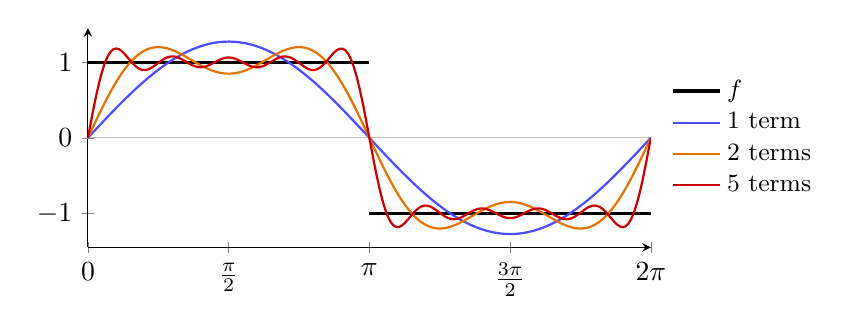
\begin{tikzpicture}
\begin{axis}[width=0.72\textwidth,height=0.36\textwidth,xmin=0,xmax=6.2832,ymin=-1.45,ymax=1.45,
  axis lines=left,xtick={0,1.5708,3.1416,4.7124,6.2832},
  xticklabels={$0$,$\tfrac\pi2$,$\pi$,$\tfrac{3\pi}2$,$2\pi$},ytick={-1,1},
  extra y ticks={0},extra y tick style={grid=major,grid style={gray!50}},
  every axis plot/.append style={samples=200,domain=0:6.2832},
  legend style={draw=none,font=\small,at={(1.02,0.5)},anchor=west},legend cell align=left]
  \addplot[black,very thick,domain=0:3.1416,samples=2] {1};
  \addlegendentry{$f$}
  \addplot[black,very thick,domain=3.1416:6.2832,samples=2,forget plot] {-1};
  \addplot[blue!70,thick] {4/pi*sin(deg(x))};
  \addlegendentry{1 term}
  \addplot[orange!90!black,thick] {4/pi*(sin(deg(x))+sin(deg(3*x))/3)};
  \addlegendentry{2 terms}
  \addplot[red!80!black,thick] {4/pi*(sin(deg(x))+sin(deg(3*x))/3+sin(deg(5*x))/5+sin(deg(7*x))/7+sin(deg(9*x))/9)};
  \addlegendentry{5 terms}
\end{axis}
\end{tikzpicture}
\caption{The square wave of Example~\ref{ex:u26-square} and the partial sums of its Fourier
series with $1$, $2$ and $5$ nonzero terms. Each added term is the projection of $f$ onto one
more basis function; the sums close in on $f$ except near the jumps, where an overshoot of
about $18\%$ of the jump's half-height persists (the Gibbs phenomenon).}
\label{fig:u26-square}
\end{figure}

\begin{trap}
The inner product of functions needs the integral over a full period, here $[0,2\pi]$.
Over other intervals the sines and cosines are generally \emph{not} orthogonal (for example
$\int_0^{\pi/2}\sin x\cos x\,dx=\tfrac12$), and the coefficient formulas fail. Also remember
the different normalization of $a_0$: the constant function has squared length $2\pi$, not
$\pi$.
\end{trap}

\subsection{Exercises}

\begin{exercise}[A jumping particle]\label{exr:u26-particle}
A particle jumps between positions $A$ and $B$. From $A$ it stays with probability $0.6$ and
jumps to $B$ with probability $0.4$; from $B$ it jumps to $A$ with probability $0.2$ and
stays with probability $0.8$. It starts at $A$. Find its probability vector after one step,
after $n$ steps, and in the limit.
\end{exercise}
\begin{solution}
With $\vb{p}=(\text{prob.\ at }A,\text{prob.\ at }B)$, the Markov matrix is
$M=\left[\begin{smallmatrix} 0.6&0.2\\ 0.4&0.8\end{smallmatrix}\right]$ and
$\vb{p}_0=(1,0)$. One step: $\vb{p}_1=M\vb{p}_0=(0.6,0.4)$. The eigenvalues are $1$ and
(trace $1.4$) $0.4$, with eigenvectors $(1,2)$ (from
$M-I=\left[\begin{smallmatrix} -0.4&0.2\\ 0.4&-0.2\end{smallmatrix}\right]$) and $(1,-1)$.
Matching $(1,0)=c_1(1,2)+c_2(1,-1)$ gives $c_1=\tfrac13$, $c_2=\tfrac23$, so
\[
  \vb{p}_n=\frac13\begin{bmatrix} 1\\ 2\end{bmatrix}+\frac23(0.4)^{n}\begin{bmatrix} 1\\ -1\end{bmatrix}
  =\frac13\begin{bmatrix} 1+2(0.4)^{n}\\ 2-2(0.4)^{n}\end{bmatrix}.
\]
For $n=1$ this is $(0.6,0.4)$ again. As $n\to\infty$, $\vb{p}_n\to(\tfrac13,\tfrac23)$: the
particle forgets where it started.
\end{solution}

\begin{exercise}[Completing a Markov matrix]\label{exr:u26-complete}
Complete the first two rows
$\left[\begin{smallmatrix} 0.7&0.1&0.2\\ 0.1&0.6&0.3\end{smallmatrix}\right]$ to a $3\times3$
Markov matrix and find its steady-state eigenvector. Why is $(1,1,\dots,1)$ the steady state of
every symmetric Markov matrix?
\end{exercise}
\begin{solution}
Each column must add to $1$, so the third row is $(0.2,\,0.3,\,0.5)$. The completed matrix is
symmetric, so its rows also add to $1$; then every row of $A-I$ adds to $0$, which says
$(A-I)(1,1,1)=\vb{0}$. The steady state is $(1,1,1)$, or $(\tfrac13,\tfrac13,\tfrac13)$ as
probabilities. The same argument works for any symmetric Markov matrix: symmetry turns the
column sums into row sums, so $A\vb{1}=\vb{1}$.
\end{solution}

\begin{exercise}[Which kinds of matrix?]\label{exr:u26-classify}
Decide which of these properties hold for
$A=\left[\begin{smallmatrix} 0&0&1\\ 0&1&0\\ 1&0&0\end{smallmatrix}\right]$ and
$B=\tfrac13\left[\begin{smallmatrix} 1&1&1\\ 1&1&1\\ 1&1&1\end{smallmatrix}\right]$:
invertible, orthogonal, projection, permutation, diagonalizable, Markov.
\end{exercise}
\begin{solution}
$A$: $\det A=-1$, so invertible; $AA\T=I$, so orthogonal; $A^{2}=I\neq A$, so not a
projection; one $1$ in each row and column, so a permutation; symmetric, so diagonalizable
(eigenvalues $1,1,-1$ with eigenvectors $(1,0,1)$, $(0,1,0)$, $(1,0,-1)$); columns add to $1$
and entries are nonnegative, so Markov.
$B$: rank $1$, so singular and not orthogonal; $B^{2}=B$ (each entry of $B^{2}$ is
$3\cdot\tfrac19$) and $B=B\T$, so it is the projection onto the line through $(1,1,1)$; not a
permutation; diagonalizable (eigenvalues $1,0,0$ with eigenvectors $(1,1,1)$ and the plane
$x+y+z=0$); Markov, since its columns add to $1$.
\end{solution}

\begin{exercise}[Fourier series of a ramp]\label{exr:u26-ramp}
Find the Fourier coefficients of $f(x)=x$ on $0\le x<2\pi$ (extended with period $2\pi$).
\end{exercise}
\begin{solution}
$a_0=\frac1{2\pi}\int_0^{2\pi}x\,dx=\frac{1}{2\pi}\cdot2\pi^{2}=\pi$, the average value.
Integrating by parts with $k\ge1$,
\begin{align*}
  \int_0^{2\pi}x\cos kx\,dx&=\Bigl[\frac{x\sin kx}{k}\Bigr]_0^{2\pi}-\int_0^{2\pi}\frac{\sin kx}{k}\,dx=0-0=0,\\
  \int_0^{2\pi}x\sin kx\,dx&=\Bigl[-\frac{x\cos kx}{k}\Bigr]_0^{2\pi}+\int_0^{2\pi}\frac{\cos kx}{k}\,dx=-\frac{2\pi}{k}+0.
\end{align*}
So $a_k=0$ and $b_k=-2/k$:
$x=\pi-2\bigl(\sin x+\tfrac12\sin2x+\tfrac13\sin3x+\cdots\bigr)$ for $0<x<2\pi$.
\end{solution}

% unit: u27
% sources: sources/002-exam-2-review.txt, sources/021-exam-2-review.txt, sources/100-mit18-06scf11-ses2-12sum-pdf-download-file.txt, sources/003-exam-2-problem-solving.txt
\section{Exam 2 review}\label{sec:u27}

Part II is the heart of the course. It started from orthogonality and least squares, built
the determinant, and arrived at eigenvalues and powers of a matrix. This section gathers the
facts to have at your fingertips for the second exam, lists the quick checks that catch most
errors, and then works through review problems of the kind the exam asks, most of them from
old 18.06 exams. The exam itself covers Sections~\ref{sec:u16}--\ref{sec:u24}; differential
equations and Markov matrices (Sections~\ref{sec:u25}--\ref{sec:u26}) build on the same
ideas and are tested later.

\subsection{What to know}

\paragraph{Orthogonality and projections (Sections~\ref{sec:u16}--\ref{sec:u18}).}
The row space is orthogonal to the nullspace, and the column space is orthogonal to the left
nullspace.
Projecting $\vb{b}$ onto the line through $\vb{a}$ gives
$\vb{p}=\dfrac{\vb{a}\T\vb{b}}{\vb{a}\T\vb{a}}\,\vb{a}$ and $P=\dfrac{\vb{a}\vb{a}\T}{\vb{a}\T\vb{a}}$.
Projecting onto the column space of $A$ (independent columns): solve the normal equations
$A\T A\hat{\vb{x}}=A\T\vb{b}$, then $\vb{p}=A\hat{\vb{x}}$ and
$P=A(A\T A)^{-1}A\T$, with $P^{2}=P=P\T$. The error $\vb{e}=\vb{b}-\vb{p}$ is perpendicular
to every column of $A$. Least squares chooses $\hat{\vb{x}}$ to minimize
$\|A\vb{x}-\vb{b}\|^{2}$, and the answer is exactly this projection.

\paragraph{Orthonormal columns and Gram--Schmidt (Section~\ref{sec:u19}).}
$Q$ has orthonormal columns exactly when $Q\T Q=I$; then the projection onto its column space
is $QQ\T$, and a square $Q$ has $Q^{-1}=Q\T$. Gram--Schmidt subtracts from each new vector its
projections onto the earlier \emph{orthogonal} directions, then normalizes; the result is
$A=QR$ with $R$ upper triangular.

\paragraph{Determinants (Sections~\ref{sec:u20}--\ref{sec:u22}).}
Three properties define $\det$: $\det I=1$; exchanging rows reverses the sign; $\det$ is
linear in each row separately. Consequences: equal rows or a zero row give $0$; subtracting a
multiple of one row from another changes nothing; triangular matrices give the product of the
diagonal; $\det A=0$ exactly when $A$ is singular; $\det AB=\det A\det B$; $\det A\T=\det A$.
The big formula has $n!$ signed terms, one entry from each row and column. The cofactor
expansion is $\det A=\sum_j a_{ij}C_{ij}$, and it leads to $A^{-1}=C\T/\det A$, Cramer's rule
and $|\det A|=$ volume.

\paragraph{Eigenvalues (Sections~\ref{sec:u23}--\ref{sec:u24}).}
Solve $\det(A-\lambda I)=0$, then find $\Nul{A-\lambda I}$. The sum of the eigenvalues is the
trace, the product is the determinant. With $n$ independent eigenvectors,
$A=X\Lambda X^{-1}$, $A^{k}=X\Lambda^{k}X^{-1}$, and
$\vb{u}_k=A^{k}\vb{u}_0=\sum c_i\lambda_i^{k}\vb{x}_i$ where $X\vb{c}=\vb{u}_0$. Distinct
eigenvalues guarantee independent eigenvectors; a repeated eigenvalue may not.

\subsection{Quick checks}

An exam rewards answers that are checked as they are produced. The cheapest checks:
\begin{itemize}
  \item eigenvalues: their sum must equal the trace and their product the determinant, and
  $A\vb{x}=\lambda\vb{x}$ can be verified in seconds;
  \item projections: $P^{2}=P$, $P\T=P$, $P\vb{a}=\vb{a}$ for vectors already in the
  subspace, and the error must be perpendicular to the subspace;
  \item Gram--Schmidt: each new vector must have zero dot product with the earlier ones;
  \item inverses and factorizations: substitute $k=1$ into a formula for $A^{k}$, multiply
  $A\,C\T$ to see $(\det A)I$, and expand a determinant along a second row or column.
\end{itemize}

\subsection{Solved review problems}

\begin{example}[Projection onto a line, and its powers]\label{ex:u27-projection}
Let $\vb{a}=(2,1,2)$. (a) Find the projection matrix $P$ onto the line through $\vb{a}$.
(b) Find its rank, column space and eigenvalues, and an eigenvector for each eigenvalue.
(c) Solve $\vb{u}_{k+1}=P\vb{u}_k$ with $\vb{u}_0=(9,9,0)$.

(a) Here $\vb{a}\T\vb{a}=9$, so
\[
  P=\frac{\vb{a}\vb{a}\T}{\vb{a}\T\vb{a}}=\frac19\begin{bmatrix} 4&2&4\\ 2&1&2\\ 4&2&4\end{bmatrix}.
\]

(b) Every column is a multiple of $\vb{a}$, so $\rank P=1$ and $\Col{P}$ is the line through
$\vb{a}$. A rank-one $3\times3$ matrix has a two-dimensional nullspace, so $\lambda=0$ is an
eigenvalue twice, with eigenvectors such as $(1,-2,0)$ and $(1,0,-1)$, the vectors
perpendicular to $\vb{a}$. The trace $\tfrac{4+1+4}{9}=1$ gives the third eigenvalue
$\lambda=1$, with eigenvector $\vb{a}$ itself: $P\vb{a}=\vb{a}(\vb{a}\T\vb{a})/9=\vb{a}$.

(c) The first step projects $\vb{u}_0$ onto the line:
\[
  \vb{u}_1=P\vb{u}_0=\frac{\vb{a}\T\vb{u}_0}{\vb{a}\T\vb{a}}\,\vb{a}=\frac{18+9+0}{9}\,\vb{a}=3\vb{a}=(6,3,6).
\]
Since $\vb{u}_1$ is already on the line, projecting again changes nothing: $P^{2}=P$, so
$\vb{u}_k=P^{k}\vb{u}_0=P\vb{u}_0=(6,3,6)$ for every $k\ge1$. In the eigenvector language of
Section~\ref{sec:u24}, $\vb{u}_0=3\vb{a}+(3,6,-6)$, where $(3,6,-6)$ is perpendicular to
$\vb{a}$ and has $\lambda=0$; that part disappears after one step and the $\lambda=1$ part
$3\vb{a}$ stays forever. For a matrix that is not a projection one would find all eigenvalues
and eigenvectors and use $\vb{u}_k=\sum c_i\lambda_i^{k}\vb{x}_i$.
\end{example}

\begin{example}[Best line through the origin]\label{ex:u27-leastsq}
Fit the line $y=Dt$ to the data points $(t,y)=(1,4)$, $(2,5)$, $(3,8)$, and say what vector
is projected onto what line.

The three equations $1\cdot D=4$, $2\cdot D=5$, $3\cdot D=8$ form $A\vb{x}=\vb{b}$ with a
single column $A=(1,2,3)$ and $\vb{b}=(4,5,8)$; they have no solution. The normal equation is
\[
  A\T A\,\hat D=A\T\vb{b}:\qquad 14\,\hat D=4+10+24=38,\qquad \hat D=\frac{19}{7}\approx2.71 .
\]
There are two pictures (Figure~\ref{fig:u27-fit}). In the $ty$-plane we fit a line to three
points; the errors are the vertical distances. In $\R^{3}$ we project the vector
$\vb{b}=(4,5,8)$ onto the line through $(1,2,3)$, the column space of $A$:
$\vb{p}=\tfrac{19}{7}(1,2,3)=\tfrac17(19,38,57)$ and
$\vb{e}=\vb{b}-\vb{p}=\tfrac17(9,-3,-1)$. Check: $\vb{e}\cdot(1,2,3)=\tfrac17(9-6-3)=0$.
The components of $\vb{e}$ are exactly the vertical errors in the first picture.
\end{example}

\begin{figure}[ht]\centering
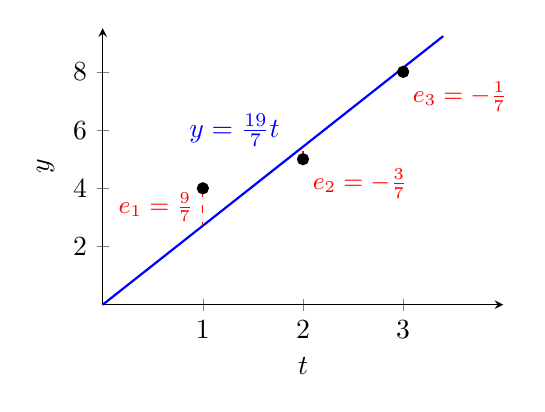
\begin{tikzpicture}
\begin{axis}[width=0.55\textwidth,height=0.42\textwidth,xmin=0,xmax=4,ymin=0,ymax=9.5,
  axis lines=left,xlabel={$t$},ylabel={$y$},xtick={1,2,3},ytick={2,4,6,8},clip=false]
  \addplot[blue,thick,domain=0:3.4] {19/7*x} node[pos=0.55,above left] {$y=\tfrac{19}{7}t$};
  \addplot[red,dashed] coordinates {(1,4) (1,19/7)};
  \addplot[red,dashed] coordinates {(2,5) (2,38/7)};
  \addplot[red,dashed] coordinates {(3,8) (3,57/7)};
  \addplot[only marks,mark=*,mark size=2pt] coordinates {(1,4) (2,5) (3,8)};
  \node[left,red,font=\small] at (axis cs:1,3.35) {$e_1=\tfrac97$};
  \node[below right,red,font=\small] at (axis cs:2,5) {$e_2=-\tfrac37$};
  \node[below right,red,font=\small] at (axis cs:3,8) {$e_3=-\tfrac17$};
\end{axis}
\end{tikzpicture}
\caption{The least-squares line through the origin for Example~\ref{ex:u27-leastsq}. The
vertical errors $e_i=y_i-\tfrac{19}{7}t_i$ are the components of the error vector
$\vb{e}=\vb{b}-\vb{p}$, which is perpendicular to the column $(1,2,3)$ in $\R^{3}$.}
\label{fig:u27-fit}
\end{figure}

\begin{example}[Gram--Schmidt in a plane]\label{ex:u27-gs}
The vectors $\vb{a}_1=(1,2,3)$ and $\vb{a}_2=(1,1,1)$ span a plane. Find two orthogonal
vectors in it, then an orthonormal pair.

Keep $\vb{a}_1$. From $\vb{a}_2$ subtract its projection onto $\vb{a}_1$:
\[
  \vb{B}=\vb{a}_2-\frac{\vb{a}_1\T\vb{a}_2}{\vb{a}_1\T\vb{a}_1}\,\vb{a}_1
  =\begin{bmatrix} 1\\ 1\\ 1\end{bmatrix}-\frac{6}{14}\begin{bmatrix} 1\\ 2\\ 3\end{bmatrix}
  =\begin{bmatrix} 1-\tfrac37\\ 1-\tfrac67\\ 1-\tfrac97\end{bmatrix}
  =\frac17\begin{bmatrix} 4\\ 1\\ -2\end{bmatrix}.
\]
Check: $\vb{a}_1\cdot(4,1,-2)=4+2-6=0$. Dividing by the lengths $\sqrt{14}$ and
$\sqrt{16+1+4}=\sqrt{21}$ gives the orthonormal pair
$\vb{q}_1=(1,2,3)/\sqrt{14}$, $\vb{q}_2=(4,1,-2)/\sqrt{21}$. The square roots appear only in
this last step, so it pays to postpone it.
\end{example}

\begin{example}[What the eigenvalues alone tell]\label{ex:u27-eigfacts}
A $4\times4$ matrix $A$ has eigenvalues $\lambda_1,\lambda_2,\lambda_3,\lambda_4$. When is it
invertible? What are $\det A^{-1}$ and $\tr(A+I)$?

$A$ is invertible exactly when no $\lambda_i$ is $0$: an eigenvalue $0$ means a nonzero vector
in the nullspace, and $\det A=\lambda_1\lambda_2\lambda_3\lambda_4$. The eigenvalues of
$A^{-1}$ are $1/\lambda_i$ (Section~\ref{sec:u23}), so
$\det A^{-1}=\dfrac{1}{\lambda_1\lambda_2\lambda_3\lambda_4}$. Adding $I$ adds $1$ to every
eigenvalue (Section~\ref{sec:u23}), so
$\tr(A+I)=\lambda_1+\lambda_2+\lambda_3+\lambda_4+4$, which is also $\tr A+4$ directly.
\end{example}

\begin{example}[Tridiagonal determinants repeat with period six]\label{ex:u27-tridiag}
Let $A_n$ be the $n\times n$ tridiagonal matrix with $1$'s on the diagonal and on both
neighbouring diagonals, and $D_n=\det A_n$. Find a recurrence for $D_n$ and solve it.

\emph{Recurrence.} Expand along the first row, which has $1$'s in columns~1 and~2 only. The
$(1,1)$ cofactor is $D_{n-1}$. The $(1,2)$ cofactor is $-1$ times the determinant of $A_n$
without row~1 and column~2; that matrix has first column $(1,0,\dots,0)$, and expanding
down it leaves $A_{n-2}$. So
\[
  D_n=D_{n-1}-D_{n-2},\qquad D_1=1,\quad D_2=\begin{vmatrix} 1&1\\ 1&1\end{vmatrix}=0 .
\]
\emph{As a matrix system.} With $\vb{u}_n=(D_n,D_{n-1})$,
$\vb{u}_n=\left[\begin{smallmatrix} 1&-1\\ 1&0\end{smallmatrix}\right]\vb{u}_{n-1}$. The
characteristic equation is $\lambda^{2}-\lambda+1=0$, so
\[
  \lambda=\frac{1\pm\sqrt{1-4}}{2}=\frac12\pm\frac{\sqrt3}{2}\,i=e^{\pm i\pi/3}.
\]
Both have $|\lambda|^{2}=\tfrac14+\tfrac34=1$: the sequence neither grows nor decays. Since
$\lambda^{6}=e^{\pm2\pi i}=1$, the matrix $M=\left[\begin{smallmatrix} 1&-1\\ 1&0\end{smallmatrix}\right]$
is diagonalizable with $\Lambda^{6}=I$, so $M^{6}=X\Lambda^{6}X^{-1}=I$ and the sequence
repeats every six steps. Running the recurrence:
\[
  D_1,\dots,D_6=1,\;0,\;-1,\;-1,\;0,\;1,\qquad\text{then } D_7=1,\ D_8=0,\dots
\]
so $D_n$ depends only on $n$ modulo $6$.
\end{example}

\begin{example}[A family of symmetric matrices]\label{ex:u27-family}
Let $A_n$ be symmetric with zeros on the diagonal and $1,2,\dots,n-1$ just above and below
it, for instance
\[
  A_3=\begin{bmatrix} 0&1&0\\ 1&0&2\\ 0&2&0\end{bmatrix},\qquad
  A_4=\begin{bmatrix} 0&1&0&0\\ 1&0&2&0\\ 0&2&0&3\\ 0&0&3&0\end{bmatrix}.
\]
(a) Find the projection matrix onto $\Col{A_3}$. (b) Find the eigenvalues and eigenvectors of
$A_3$. (c) Find the projection onto $\Col{A_4}$. (d) Show that $A_n$ is singular for odd $n$ and
invertible for even $n$.

(a) Column~3 is twice column~1, so $\Col{A_3}$ is the plane spanned by $(0,1,0)$ and
$(1,0,2)$. These two columns are already orthogonal, so $P$ is the sum of the two
projections onto lines:
\[
  P=\begin{bmatrix} 0\\ 1\\ 0\end{bmatrix}\begin{bmatrix} 0&1&0\end{bmatrix}
   +\frac15\begin{bmatrix} 1\\ 0\\ 2\end{bmatrix}\begin{bmatrix} 1&0&2\end{bmatrix}
  =\begin{bmatrix} \tfrac15&0&\tfrac25\\ 0&1&0\\ \tfrac25&0&\tfrac45\end{bmatrix}.
\]
The formula $A(A\T A)^{-1}A\T$ with these two columns gives the same matrix. Check: $P$
fixes all three columns of $A_3$.

(b) $\det(A_3-\lambda I)=-\lambda^{3}+5\lambda=-\lambda(\lambda^{2}-5)$, so
$\lambda=0,\sqrt5,-\sqrt5$ (trace check: the sum is $0$). The eigenvectors are
$(-2,0,1)$ for $0$ and $(1,\pm\sqrt5,2)$ for $\pm\sqrt5$; for instance
$A_3(1,\sqrt5,2)=(\sqrt5,\,5,\,2\sqrt5)=\sqrt5\,(1,\sqrt5,2)$. The eigenvector
$(-2,0,1)$ spans the nullspace, perpendicular to $\Col{A_3}$, so $P=I-\tfrac15(-2,0,1)(-2,0,1)\T$
is another route to (a).

(c) If $A_4$ is invertible, its column space is all of $\R^{4}$ and the projection is
$P=I$. Expanding along row~1 (only the entry $1$ in column~2), then down the first column of
the resulting $3\times3$ minor,
\[
  \det A_4=-1\cdot\begin{vmatrix} 1&2&0\\ 0&0&3\\ 0&3&0\end{vmatrix}
  =-1\cdot1\cdot\begin{vmatrix} 0&3\\ 3&0\end{vmatrix}=-1\cdot(-9)=9\neq0 .
\]
So $P=I$.

(d) Expand $D_n=\det A_n$ along the last row, whose only nonzero entry is $n-1$ in column
$n-1$. Its minor has last column $(0,\dots,0,n-1)$; expanding down that column leaves
$A_{n-2}$. With the sign $(-1)^{n+(n-1)}=-1$,
\[
  D_n=-(n-1)^{2}\,D_{n-2},\qquad D_1=0,\quad D_2=-1 .
\]
So $D_n=0$ for every odd $n$, and for even $n$ the determinant is
$\pm\bigl(1\cdot3\cdot5\cdots(n-1)\bigr)^{2}\neq0$: for example $D_4=-9D_2=9$ and
$D_6=-25D_4=-225$.
\end{example}

\begin{example}[The big formula when many entries are zero]\label{ex:u27-bigformula}
For the matrix below, find $\det A$ from the big formula, the cofactors
$C_{11},\dots,C_{14}$, and the first column of $A^{-1}$:
\[
  A=\begin{bmatrix} 1&2&3&4\\ 5&6&7&8\\ 0&0&9&10\\ 0&0&11&12\end{bmatrix}.
\]

\emph{Big formula.} Of the $24$ terms, only those avoiding the four zeros survive. Rows~3
and~4 must use columns~3 and~4, so rows~1 and~2 use columns~1 and~2: four terms in all. A
term's sign is that of its column permutation:
\[
  \det A=+1\cdot6\cdot9\cdot12-1\cdot6\cdot10\cdot11-2\cdot5\cdot9\cdot12+2\cdot5\cdot10\cdot11
  =648-660-1080+1100=8 .
\]
(The permutations are $(1,2,3,4)$, $(1,2,4,3)$, $(2,1,3,4)$ and $(2,1,4,3)$, with $0$, $1$, $1$
and $2$ exchanges.)

\emph{Cofactors.} $C_{11}=\det\left[\begin{smallmatrix} 6&7&8\\ 0&9&10\\ 0&11&12\end{smallmatrix}\right]=6(108-110)=-12$
and $C_{12}=-\det\left[\begin{smallmatrix} 5&7&8\\ 0&9&10\\ 0&11&12\end{smallmatrix}\right]=-5(-2)=10$,
each expanded down its first column. $C_{13}=C_{14}=0$ without computation: their minors have
first two columns $(5,0,0)$ and $(6,0,0)$, which are dependent. Check:
$\det A=1\cdot(-12)+2\cdot10+0+0=8$.

\emph{First column of $A^{-1}$.} By the formula $A^{-1}=C\T/\det A$ of Section~\ref{sec:u22} it is the first row of
cofactors divided by the determinant:
\[
  \frac{1}{\det A}\,(C_{11},C_{12},C_{13},C_{14})=\frac18\,(-12,10,0,0)=\Bigl(-\frac32,\frac54,0,0\Bigr).
\]
A third check: $A$ is block triangular, and
$\det\left[\begin{smallmatrix} 1&2\\ 5&6\end{smallmatrix}\right]\det\left[\begin{smallmatrix} 9&10\\ 11&12\end{smallmatrix}\right]=(-4)(-2)=8$.
\end{example}

\subsection{Exercises}

\begin{exercise}\label{exr:u27-line}
Fit the best straight line $y=C+Dt$ to the points $(-1,1)$, $(0,2)$, $(1,4)$, and find the
error vector.
\end{exercise}
\begin{solution}
$A=\left[\begin{smallmatrix} 1&-1\\ 1&0\\ 1&1\end{smallmatrix}\right]$, $\vb{b}=(1,2,4)$.
Because the times add to zero, the columns of $A$ are orthogonal and
$A\T A=\left[\begin{smallmatrix} 3&0\\ 0&2\end{smallmatrix}\right]$, while $A\T\vb{b}=(7,3)$.
So $\hat C=\tfrac73$, $\hat D=\tfrac32$. The fitted values are
$\tfrac73+\tfrac32t=\tfrac56,\tfrac73,\tfrac{23}{6}$ at $t=-1,0,1$, and
$\vb{e}=(1,2,4)-(\tfrac56,\tfrac{14}{6},\tfrac{23}{6})=(\tfrac16,-\tfrac13,\tfrac16)$, which is
perpendicular to both columns: $\tfrac16-\tfrac13+\tfrac16=0$ and $-\tfrac16+0+\tfrac16=0$.
\end{solution}

\begin{exercise}\label{exr:u27-eigalg}
A $3\times3$ matrix $A$ has eigenvalues $1,2,3$. Find $\det A$, $\tr A$, the eigenvalues of
$A^{2}-A$, and $\det(A^{2}-A)$. Is $A$ diagonalizable?
\end{exercise}
\begin{solution}
$\det A=1\cdot2\cdot3=6$ and $\tr A=6$. By Section~\ref{sec:u23} the
eigenvalues of $A^{2}-A$ are $\lambda^{2}-\lambda=0,2,6$, so $\det(A^{2}-A)=0$: the matrix
$A^{2}-A=A(A-I)$ is singular, as it must be since $A-I$ has the eigenvalue $0$. $A$ is
diagonalizable because its three eigenvalues are distinct (Section~\ref{sec:u24}).
\end{solution}

\begin{exercise}\label{exr:u27-tridiag2}
Let $T_n$ be tridiagonal with $2$'s on the diagonal and $-1$'s on the two neighbouring
diagonals. Use cofactors to show $\det T_n=2\det T_{n-1}-\det T_{n-2}$, and find $\det T_n$.
\end{exercise}
\begin{solution}
Expanding along the first row exactly as in Example~\ref{ex:u27-tridiag}: the $(1,1)$ term
gives $2\det T_{n-1}$; the $(1,2)$ entry $-1$ has cofactor $-1$ times a determinant whose
first column is $(-1,0,\dots,0)$, which equals $-\det T_{n-2}$. Altogether
$\det T_n=2\det T_{n-1}+(-1)(-1)(-\det T_{n-2})=2\det T_{n-1}-\det T_{n-2}$. With
$\det T_1=2$ and $\det T_2=4-1=3$, the recurrence gives $4,5,6,\dots$; by induction
$\det T_n=n+1$, since $2n-(n-1)=n+1$. (In matrix form, $\left[\begin{smallmatrix} 2&-1\\ 1&0\end{smallmatrix}\right]$
has the repeated eigenvalue $1$ and only one eigenvector, which is why the answer grows
linearly instead of like a power.)
\end{solution}

% unit: u28
% sources: sources/016-exam-2.txt, sources/111-mit18-06scf11-ex2-pdf-download-file.txt, sources/112-mit18-06scf11-ex2s-pdf-download-file.txt
\section{Exam 2}\label{sec:u28}

The second unit exam tests Sections~\ref{sec:u16}--\ref{sec:u24} through four problems:
determinants of matrices built from orthonormal vectors, a least-squares line, projections
and the next Gram--Schmidt vector, and a determinant that is a polynomial in one repeated
entry. Each problem is restated below and solved with the reasoning an examiner wants to see,
followed by further practice problems of the same kind. Try each problem before reading its
solution.

\subsection{The exam problems}

\begin{example}[Determinants from orthonormal vectors]\label{ex:u28-q}
Let $\vb{q}_1,\vb{q}_2,\vb{q}_3$ be orthonormal vectors in $\R^{3}$ and
$Q=\begin{bmatrix}\vb{q}_1&\vb{q}_2&\vb{q}_3\end{bmatrix}$. Find all possible values of
(a) $\det Q$; (b) $\det\begin{bmatrix}\vb{q}_1+\vb{q}_2&\vb{q}_2+\vb{q}_3&\vb{q}_3+\vb{q}_1\end{bmatrix}$;
(c) $\det Q$ times $\det\begin{bmatrix}\vb{q}_2&\vb{q}_3&\vb{q}_1\end{bmatrix}$.

(a) $Q\T Q=I$, so $(\det Q)^{2}=\det Q\T\det Q=\det I=1$ and $\det Q=\pm1$. Both values occur:
$Q=I$ gives $+1$, and $Q=\operatorname{diag}(1,1,-1)$ gives $-1$.

(b) The new columns are combinations of the old ones:
\[
  \begin{bmatrix}\vb{q}_1+\vb{q}_2&\vb{q}_2+\vb{q}_3&\vb{q}_3+\vb{q}_1\end{bmatrix}
  =Q\,M,\qquad M=\begin{bmatrix} 1&0&1\\ 1&1&0\\ 0&1&1\end{bmatrix},
\]
since column $j$ of $QM$ is $Q$ times column $j$ of $M$. Expanding along the first row,
$\det M=1\cdot(1-0)-0+1\cdot(1-0)=2$, so the determinant is $\det Q\det M=\pm2$.
Linearity in each column gives the same answer: of the eight determinants obtained by
splitting every column, all but two have a repeated column and vanish, leaving
$\det[\vb{q}_1\;\vb{q}_2\;\vb{q}_3]+\det[\vb{q}_2\;\vb{q}_3\;\vb{q}_1]=2\det Q$ by part (c).

(c) $[\vb{q}_2\;\vb{q}_3\;\vb{q}_1]$ is $Q$ with its columns cycled, which takes two
exchanges (swap columns~1 and~2, then columns~2 and~3). An even number of exchanges keeps the
determinant, so the product is $(\det Q)^{2}=1$, whichever sign $\det Q$ has.
\end{example}

\begin{example}[A least-squares line through 21 points]\label{ex:u28-21}
Measurements are taken at the $21$ times $t=-10,-9,\dots,9,10$. All are $b_i=0$ except
$b=1$ at the middle time $t=0$. (a) Find the least-squares line $C+Dt$. (b) Onto which
subspace is $\vb{b}$ projected? Give a basis, and a nonzero vector perpendicular to it.

(a) Exact fitting would require the $21$ equations $C+Dt_i=b_i$, that is
$A\vb{x}=\vb{b}$ with $\vb{x}=(C,D)$ and $A$ the $21\times2$ matrix whose columns are
$\vb{1}=(1,\dots,1)$ and $\vb{t}=(-10,\dots,10)$. The normal equations need
\[
  \vb{1}\T\vb{1}=21,\qquad \vb{1}\T\vb{t}=\sum t_i=0,\qquad
  \vb{t}\T\vb{t}=2(1^{2}+2^{2}+\dots+10^{2})=2\cdot385=770,
\]
and $A\T\vb{b}=(\vb{1}\T\vb{b},\vb{t}\T\vb{b})=(1,0)$, since the only nonzero $b_i$ sits at
$t=0$. So
\[
  \begin{bmatrix} 21&0\\ 0&770\end{bmatrix}\begin{bmatrix}\hat C\\ \hat D\end{bmatrix}
  =\begin{bmatrix} 1\\ 0\end{bmatrix},\qquad \hat C=\frac1{21},\quad \hat D=0 .
\]
The best line is the horizontal line $y=\tfrac1{21}$ (Figure~\ref{fig:u28-21}). Because the
times are symmetric about $0$, the two columns of $A$ are orthogonal and the normal equations
uncouple: $\hat C$ is the average of the $b_i$, and $\hat D=\vb{t}\T\vb{b}/\vb{t}\T\vb{t}=0$.
A symmetric data set cannot prefer an upward or a downward slope.

(b) $\vb{b}\in\R^{21}$ is projected onto the column space of $A$, a plane in $\R^{21}$ with
basis $\vb{1}$ and $\vb{t}$. The error vector is perpendicular to it:
\[
  \vb{e}=\vb{b}-\vb{p}=\vb{b}-\tfrac1{21}\vb{1}=\tfrac1{21}(\underbrace{-1,\dots,-1}_{10},\,20,\,\underbrace{-1,\dots,-1}_{10}).
\]
Check: its components add to $\tfrac1{21}(20-20)=0$, and $\vb{t}\T\vb{e}=0$ by symmetry. A
simpler perpendicular vector is $(1,-2,1,0,\dots,0)$: its components add to $0$, and against
$\vb{t}$ it gives $-10+18-8=0$.
\end{example}

\begin{figure}[ht]\centering
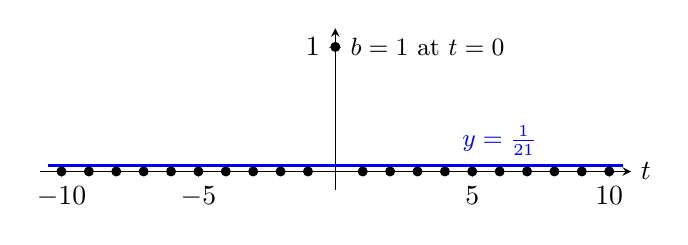
\begin{tikzpicture}
\begin{axis}[width=0.75\textwidth,height=0.3\textwidth,xmin=-10.8,xmax=10.8,ymin=-0.15,ymax=1.15,
  axis lines=middle,xlabel={$t$},xtick={-10,-5,5,10},ytick={1},
  xlabel style={anchor=west},clip=false]
  \addplot[only marks,mark=*,mark size=1.6pt] coordinates {(-10,0) (-9,0) (-8,0) (-7,0) (-6,0)
    (-5,0) (-4,0) (-3,0) (-2,0) (-1,0) (0,1) (1,0) (2,0) (3,0) (4,0) (5,0) (6,0) (7,0) (8,0)
    (9,0) (10,0)};
  \addplot[blue,thick,domain=-10.5:10.5] {1/21};
  \node[blue,above,font=\small] at (axis cs:6,0.05) {$y=\tfrac1{21}$};
  \node[right,font=\small] at (axis cs:0.2,1) {$b=1$ at $t=0$};
\end{axis}
\end{tikzpicture}
\caption{The data of Example~\ref{ex:u28-21} and its least-squares line. Twenty points sit
at $0$ and one at $1$; the best line is the horizontal line at the average height
$\tfrac1{21}$. Any tilt would help on one side of $t=0$ exactly as much as it hurts on the
other.}
\label{fig:u28-21}
\end{figure}

\begin{example}[Projections from Gram--Schmidt and the next vector]\label{ex:u28-gs}
Gram--Schmidt turns independent vectors $\vb{a}_1,\vb{a}_2,\vb{a}_3$ in $\R^{5}$ into
orthonormal $\vb{q}_1,\vb{q}_2,\vb{q}_3$. Let $A$ and $Q$ be the $5\times3$ matrices with
these columns. (a) Give formulas for the projection matrices $P_A$ and $P_Q$ onto their
column spaces. (b) Is $P_Q=P_A$? What is $P_QQ$? What is $\det P_Q$? (c) A fourth vector
$\vb{a}_4$ is added, with $\vb{a}_1,\dots,\vb{a}_4$ independent. Which of these is the next
Gram--Schmidt vector $\vb{q}_4$?
\[
  \text{(1)}\ \frac{P_Q\vb{a}_4}{\|P_Q\vb{a}_4\|},\qquad
  \text{(2)}\ \frac{\vb{w}}{\|\vb{w}\|}\ \text{with}\
  \vb{w}=\vb{a}_4-\frac{\vb{a}_4\T\vb{a}_1}{\vb{a}_1\T\vb{a}_1}\vb{a}_1
  -\frac{\vb{a}_4\T\vb{a}_2}{\vb{a}_2\T\vb{a}_2}\vb{a}_2
  -\frac{\vb{a}_4\T\vb{a}_3}{\vb{a}_3\T\vb{a}_3}\vb{a}_3,\qquad
  \text{(3)}\ \frac{\vb{a}_4-P_A\vb{a}_4}{\|\vb{a}_4-P_A\vb{a}_4\|}.
\]

(a) $P_A=A(A\T A)^{-1}A\T$ and $P_Q=Q(Q\T Q)^{-1}Q\T=QQ\T$, because $Q\T Q=I$.

(b) Yes, $P_Q=P_A$. Gram--Schmidt never leaves the span: each $\vb{q}_j$ is a combination
of $\vb{a}_1,\dots,\vb{a}_j$ and each $\vb{a}_j$ a combination of $\vb{q}_1,\dots,\vb{q}_j$,
so $\Col{Q}=\Col{A}$, and the projection onto a subspace depends only on the subspace, not on
the basis used to describe it. (Substituting $A=QR$ into $A(A\T A)^{-1}A\T$ and cancelling
also works.) Next, $P_QQ=QQ\T Q=Q$: vectors already in the subspace are not moved. Finally
$\det P_Q=0$: $P_Q$ is $5\times5$ with rank $3$, and every vector perpendicular to $\Col{Q}$ is
sent to $\vb{0}$.

(c) Choice (3). The vector $\vb{a}_4-P_A\vb{a}_4$ is the error of projecting $\vb{a}_4$ onto
$\Col{A}$, so it is perpendicular to $\vb{q}_1,\vb{q}_2,\vb{q}_3$; it is nonzero because
$\vb{a}_4$ is not in $\Col{A}$; dividing by its length makes it a unit vector. This is
exactly what Gram--Schmidt computes, usually written
$\vb{a}_4-(\vb{q}_1\T\vb{a}_4)\vb{q}_1-(\vb{q}_2\T\vb{a}_4)\vb{q}_2-(\vb{q}_3\T\vb{a}_4)\vb{q}_3$.
Choice (1) is the projection itself, which lies \emph{in} the old subspace, the opposite of
what we want. Choice (2) is the tempting one: it would be right with the orthogonal
$\vb{q}_i$ in place of the $\vb{a}_i$, but subtracting projections onto lines that are not
perpendicular to each other does not leave a vector perpendicular to all of them.
\end{example}

The failure of choice (2) is easy to see in a small case. In $\R^{3}$ take
$\vb{a}_1=(1,0,0)$, $\vb{a}_2=(1,1,0)$ and a new vector $\vb{a}_3=(1,1,1)$. The formula of
choice (2) gives
$\vb{w}=(1,1,1)-\tfrac11(1,0,0)-\tfrac22(1,1,0)=(-1,0,1)$, and $\vb{w}\cdot\vb{a}_1=-1\neq0$.
The correct $\vb{a}_3-P_A\vb{a}_3$ is $(0,0,1)$, perpendicular to the whole plane of
$\vb{a}_1,\vb{a}_2$.

\begin{example}[A determinant that is a polynomial]\label{ex:u28-poly}
A $4\times4$ matrix has the same number $x$ in every position of its first row and first
column (the exam writes $\times$ for it); the other nine entries are fixed numbers.
(a) $\det A$ is a polynomial in $x$. What is its largest possible degree? (b) If the nine
numbers form the $3\times3$ identity, find $\det A$ and the values of $x$ that make it zero.

(a) Degree at most $2$. Each term of the big formula takes exactly one entry from each row
and each column. All the $x$'s lie in row~1 or column~1, so a term can contain at most one
$x$ from row~1 and at most one from column~1; the corner entry $a_{11}=x$ uses up both. So
each term has at most two factors $x$. Part (b) shows the degree $2$ is actually reached.

(b) The matrix is
\[
  A=\begin{bmatrix} x&x&x&x\\ x&1&0&0\\ x&0&1&0\\ x&0&0&1\end{bmatrix}.
\]
Subtract $x$ times rows~2, 3 and~4 from row~1; this does not change the determinant and
clears the last three entries of row~1, leaving $x-3x^{2}$ in the corner. The result is
lower triangular, so
\[
  \det A=(x-3x^{2})\cdot1\cdot1\cdot1=x(1-3x).
\]
It is zero for $x=0$ (a zero row) and for $x=\tfrac13$. For $x=\tfrac13$ the dependence is
visible: rows~2, 3, 4 add to $(1,1,1,1)$, which is $3$ times row~1.
\end{example}

\begin{trap}
In Example~\ref{ex:u28-poly}(a) it is tempting to count the seven $x$'s and guess degree $7$,
or to count four per row and guess $4$. The big formula is the right tool for questions about
the \emph{form} of a determinant: one entry per row and per column limits how many $x$'s can
meet in one term.
\end{trap}

\subsection{Further practice}

\begin{exercise}\label{exr:u28-q2}
With $\vb{q}_1,\vb{q}_2,\vb{q}_3$ orthonormal in $\R^{3}$, find the determinants
\[
  \det\begin{bmatrix}\vb{q}_1-\vb{q}_2&\vb{q}_2-\vb{q}_3&\vb{q}_3-\vb{q}_1\end{bmatrix}
  \qquad\text{and}\qquad
  \det\begin{bmatrix}\vb{q}_1+\vb{q}_2&\vb{q}_1-\vb{q}_2&\vb{q}_3\end{bmatrix}.
\]
\end{exercise}
\begin{solution}
The three columns of the first matrix add to $\vb{0}$, so they are dependent and the
determinant is $0$. For the second, write it as $QM$ with
$M=\left[\begin{smallmatrix} 1&1&0\\ 1&-1&0\\ 0&0&1\end{smallmatrix}\right]$;
$\det M=1\cdot(-1)-1\cdot1=-2$, so the determinant is $-2\det Q=\mp2$. Geometrically, the
first two columns are perpendicular with length $\sqrt2$ each, so the box has volume
$\sqrt2\cdot\sqrt2\cdot1=2$, in agreement with the volume interpretation of Section~\ref{sec:u22}.
\end{solution}

\begin{exercise}\label{exr:u28-5pts}
Measurements at $t=-2,-1,0,1,2$ are $\vb{b}=(0,0,0,0,1)$. Find the least-squares line
$C+Dt$ and check that the error is perpendicular to both columns of $A$.
\end{exercise}
\begin{solution}
The columns $\vb{1}$ and $\vb{t}=(-2,-1,0,1,2)$ are orthogonal, with $\vb{1}\T\vb{1}=5$ and
$\vb{t}\T\vb{t}=10$; also $\vb{1}\T\vb{b}=1$ and $\vb{t}\T\vb{b}=2$. So $\hat C=\tfrac15$ and
$\hat D=\tfrac2{10}=\tfrac15$: the line is $y=\tfrac15(1+t)$. Its values at the five times are
$\vb{p}=\tfrac15(-1,0,1,2,3)$, so $\vb{e}=\vb{b}-\vb{p}=\tfrac15(1,0,-1,-2,2)$. Check:
$1+0-1-2+2=0$ and $-2+0+0-2+4=0$. Unlike Example~\ref{ex:u28-21}, the lone nonzero
measurement is off-centre, so the line tilts toward it.
\end{solution}

\begin{exercise}\label{exr:u28-poly2}
Repeat Example~\ref{ex:u28-poly}(b) when the nine numbers form $2I$ instead of $I$.
\end{exercise}
\begin{solution}
Subtract $\tfrac{x}{2}$ times rows~2, 3, 4 from row~1. The corner becomes
$x-3\cdot\tfrac{x}{2}\cdot x=x-\tfrac32x^{2}$, the rest of row~1 becomes $0$, and the
remaining diagonal is $2,2,2$. So $\det A=8\bigl(x-\tfrac32x^{2}\bigr)=8x-12x^{2}=4x(2-3x)$,
which vanishes for $x=0$ and $x=\tfrac23$. The degree is again $2$, as part (a) of the
example predicts.
\end{solution}

\part{Positive definite matrices and applications}
% unit: u29
% sources: sources/073-symmetric-matrices-and-positive-definiteness.txt, sources/049-lecture-25-symmetric-matrices-and-positive-definiteness.txt, sources/206-mit18-06scf11-ses3-1sum-pdf-download-file.txt, sources/050-problem-solving-symmetric-matrices-and-positive-definiteness.txt, sources/207-mit18-06scf11-ses3-1prob-pdf-download-file.txt, sources/208-mit18-06scf11-ses3-1sol-pdf-download-file.txt
\section{Symmetric matrices and positive definiteness}\label{sec:u29}

Part~II ended with the eigenvalue picture of a square matrix: when $A$ has $n$ independent
eigenvectors, $A=X\Lambda X^{-1}$ (Section~\ref{sec:u24}). A matrix with special structure should
have special eigenvalues and eigenvectors; Markov matrices, for instance, always have
$\lambda=1$ (Section~\ref{sec:u26}). This unit studies the most important special class,
the \emph{symmetric} matrices $A=A\T$. Two facts carry the whole unit:
\begin{itemize}
  \item the eigenvalues of a real symmetric matrix are \textbf{real};
  \item its eigenvectors can be chosen \textbf{perpendicular}, so $X$ becomes an orthogonal matrix $Q$.
\end{itemize}
Once eigenvalues are known to be real we can ask for their \emph{signs}, and a surprising
shortcut appears: the signs of the pivots are the signs of the eigenvalues. The symmetric
matrices whose eigenvalues are all positive, the positive definite matrices, are where pivots,
determinants and eigenvalues finally come together.

\subsection{Real eigenvalues}

\begin{definition}[Symmetric matrix]\label{def:u29-symmetric}
A square real matrix $A$ is \emph{symmetric} if $A\T=A$, that is $a_{ij}=a_{ji}$ for all $i,j$.
\end{definition}

A real matrix can have complex eigenvalues: the $90^\circ$ rotation
$\left[\begin{smallmatrix}0&-1\\1&0\end{smallmatrix}\right]$ has $\lambda=\pm i$. So to prove that
symmetric matrices do not, we must allow $\lambda$ and $\vb{x}$ to be complex for a moment
and see what symmetry forces. The tool is the complex conjugate: if $z=a+ib$ then
$\bar z=a-ib$ and $\bar z z=a^2+b^2\ge 0$.

\begin{lemma}[Conjugate length]\label{lem:u29-xbarx}
For a complex vector $\vb{x}=(x_1,\dots,x_n)$,
\[
  \bar{\vb{x}}\T\vb{x}=\bar x_1x_1+\cdots+\bar x_nx_n=|x_1|^2+\cdots+|x_n|^2 ,
\]
which is real, and positive unless $\vb{x}=\vb{0}$.
\end{lemma}
\begin{proof}
Each term is $\bar x_kx_k=(a_k-ib_k)(a_k+ib_k)=a_k^2+b_k^2=|x_k|^2$: the cross terms $\pm ia_kb_k$
cancel. A sum of such squares is zero only when every $a_k$ and $b_k$ is zero.
\end{proof}

Without the bar the lemma fails: for $\vb{x}=(1,i)$ we get $\vb{x}\T\vb{x}=1+i^2=0$ although
$\vb{x}\ne\vb{0}$. Section~\ref{sec:u30} builds the geometry of complex vectors on this
observation.

\begin{theorem}[Real eigenvalues]\label{thm:u29-real}
Every eigenvalue of a real symmetric matrix is real.
\end{theorem}
\begin{proof}
Let $A\vb{x}=\lambda\vb{x}$ with $\vb{x}\ne\vb{0}$, where $\lambda$ and $\vb{x}$ may be complex.
Take complex conjugates of every factor. Because $A$ is real, $\bar A=A$ and
\[
  A\bar{\vb{x}}=\bar\lambda\,\bar{\vb{x}}.
\]
(This step alone shows that the complex eigenvalues of any real matrix come in conjugate pairs
$\lambda,\bar\lambda$.) Now transpose and use $A\T=A$, which is the only place symmetry enters:
\[
  \bar{\vb{x}}\T A=\bar\lambda\,\bar{\vb{x}}\T .
\]
Multiply this on the right by $\vb{x}$, and multiply the original equation $A\vb{x}=\lambda\vb{x}$
on the left by $\bar{\vb{x}}\T$:
\[
  \bar{\vb{x}}\T A\vb{x}=\bar\lambda\,\bar{\vb{x}}\T\vb{x},
  \qquad
  \bar{\vb{x}}\T A\vb{x}=\lambda\,\bar{\vb{x}}\T\vb{x}.
\]
The left sides agree, so $(\lambda-\bar\lambda)\,\bar{\vb{x}}\T\vb{x}=0$. By
Lemma~\ref{lem:u29-xbarx}, $\bar{\vb{x}}\T\vb{x}>0$, so $\lambda=\bar\lambda$: the imaginary part
of $\lambda$ is zero.
\end{proof}

Once $\lambda$ is real, $A-\lambda I$ is a real singular matrix, so its nullspace contains real
nonzero vectors. Eigenvectors of a real symmetric matrix can therefore always be taken real.

\begin{remark}
If $A$ is complex, the same proof goes through provided $\bar A\T=A$: transposing
$\bar A\bar{\vb{x}}=\bar\lambda\bar{\vb{x}}$ gives $\bar{\vb{x}}\T\bar A\T=\bar\lambda\bar{\vb{x}}\T$,
and we need $\bar A\T=A$ to continue. So the right complex analogue of ``symmetric'' is
``equal to its conjugate transpose''. These Hermitian matrices are the subject of
Section~\ref{sec:u30}.
\end{remark}

\subsection{Perpendicular eigenvectors and the spectral theorem}

\begin{theorem}[Orthogonal eigenvectors]\label{thm:u29-orth}
If $A$ is real symmetric, $A\vb{x}=\lambda_1\vb{x}$ and $A\vb{y}=\lambda_2\vb{y}$ with
$\lambda_1\ne\lambda_2$, then $\vb{x}\T\vb{y}=0$.
\end{theorem}
\begin{proof}
Compute $\vb{x}\T A\vb{y}$ in two ways. Using $A\vb{y}=\lambda_2\vb{y}$ gives $\lambda_2\vb{x}\T\vb{y}$.
Using symmetry, $\vb{x}\T A\vb{y}=(A\T\vb{x})\T\vb{y}=(A\vb{x})\T\vb{y}=\lambda_1\vb{x}\T\vb{y}$.
Hence $(\lambda_1-\lambda_2)\vb{x}\T\vb{y}=0$, and since $\lambda_1\ne\lambda_2$, $\vb{x}\T\vb{y}=0$.
\end{proof}

When an eigenvalue is repeated there is a whole plane (or larger subspace) of eigenvectors,
and not every pair in it is perpendicular. The identity matrix is the extreme case: every
vector is an eigenvector. The correct statement is that the eigenvectors \emph{can be chosen}
perpendicular, and that there are always enough of them. That is the content of the main
theorem.

\begin{theorem}[Spectral theorem; principal axis theorem]\label{thm:u29-spectral}
Every real symmetric $n\times n$ matrix can be factored as
\[
  A=Q\Lambda Q\T ,
\]
where $Q$ is an orthogonal matrix ($Q\T Q=I$) whose columns are orthonormal eigenvectors
$\vb{q}_1,\dots,\vb{q}_n$ of $A$, and $\Lambda$ is the real diagonal matrix of eigenvalues.
Conversely, every matrix of the form $Q\Lambda Q\T$ with $\Lambda$ real diagonal is symmetric.
\end{theorem}
\begin{proof}
The converse is one line: $(Q\Lambda Q\T)\T=(Q\T)\T\Lambda\T Q\T=Q\Lambda Q\T$.

For the factorization we use induction on $n$; the case $n=1$ is trivial. The characteristic
polynomial of $A$ has at least one root $\lambda_1$, which is real by
Theorem~\ref{thm:u29-real}, with a real unit eigenvector $\vb{q}_1$. Extend $\vb{q}_1$ to an
orthonormal basis $\vb{q}_1,\vb{p}_2,\dots,\vb{p}_n$ of $\R^n$ (Gram--Schmidt,
Section~\ref{sec:u19}) and let $Q_1$ be the orthogonal matrix with these columns. The first
column of $Q_1\T AQ_1$ is $Q_1\T A\vb{q}_1=\lambda_1Q_1\T\vb{q}_1=\lambda_1\vb{e}_1$. The matrix
$Q_1\T AQ_1$ is symmetric, because $(Q_1\T AQ_1)\T=Q_1\T A\T Q_1=Q_1\T AQ_1$, so its first row is
also $\lambda_1\vb{e}_1\T$:
\[
  Q_1\T AQ_1=\begin{bmatrix}\lambda_1&\vb{0}\T\\ \vb{0}&A_2\end{bmatrix},
  \qquad A_2 \text{ symmetric of size } n-1 .
\]
By induction $A_2=Q_2\Lambda_2Q_2\T$ with $Q_2$ orthogonal. Put
$Q=Q_1\left[\begin{smallmatrix}1&\vb{0}\T\\ \vb{0}&Q_2\end{smallmatrix}\right]$, a product of
orthogonal matrices and hence orthogonal. Then
$Q\T AQ=\left[\begin{smallmatrix}\lambda_1&\vb{0}\T\\ \vb{0}&\Lambda_2\end{smallmatrix}\right]=\Lambda$,
that is $A=Q\Lambda Q\T$. Reading $AQ=Q\Lambda$ column by column shows $A\vb{q}_k=\lambda_k\vb{q}_k$.
\end{proof}

Compared with the general diagonalization $A=X\Lambda X^{-1}$, two things have improved:
the eigenvalues in $\Lambda$ are real, and the eigenvector matrix $X$ has become an orthogonal
$Q$, whose inverse is simply $Q\T$. Mathematicians call the set of eigenvalues the
\emph{spectrum}, hence the name; in mechanics the same statement is the principal axis
theorem: in the right axes (the eigenvectors) a symmetric operation does not couple the
directions together.

\begin{corollary}[A sum of projections]\label{cor:u29-projections}
If $A=Q\Lambda Q\T$ then, multiplying columns times rows,
\[
  A=\lambda_1\vb{q}_1\vb{q}_1\T+\lambda_2\vb{q}_2\vb{q}_2\T+\cdots+\lambda_n\vb{q}_n\vb{q}_n\T .
\]
Each $P_k=\vb{q}_k\vb{q}_k\T$ is the projection matrix onto the line through $\vb{q}_k$; these
projections satisfy $P_k^2=P_k$, $P_jP_k=0$ for $j\ne k$, and $P_1+\cdots+P_n=QQ\T=I$.
\end{corollary}
\begin{proof}
The product $Q(\Lambda Q\T)$ is a sum of (column $k$ of $Q$) times (row $k$ of $\Lambda Q\T$),
and row $k$ of $\Lambda Q\T$ is $\lambda_k\vb{q}_k\T$. For a unit vector the projection formula
$\vb{a}\vb{a}\T/\vb{a}\T\vb{a}$ of Section~\ref{sec:u17} reduces to $\vb{q}_k\vb{q}_k\T$. Finally
$P_jP_k=\vb{q}_j(\vb{q}_j\T\vb{q}_k)\vb{q}_k\T$ is $P_k$ when $j=k$ and $0$ otherwise.
\end{proof}

So a symmetric matrix acts on $\vb{x}$ in three moves: split $\vb{x}$ into its pieces
$(\vb{q}_k\T\vb{x})\vb{q}_k$ along perpendicular axes, stretch piece $k$ by $\lambda_k$, add.

\begin{example}[A spectral decomposition, worked in full]\label{ex:u29-spectral}
Take $A=\begin{bmatrix}1&2\\2&-2\end{bmatrix}$. The trace is $-1$ and the determinant is
$-2-4=-6$, so $\lambda^2+\lambda-6=(\lambda-2)(\lambda+3)=0$ and $\lambda_1=2$, $\lambda_2=-3$:
real, as promised.

\emph{Eigenvectors.} $A-2I=\left[\begin{smallmatrix}-1&2\\2&-4\end{smallmatrix}\right]$ has nullspace
spanned by $(2,1)$; $A+3I=\left[\begin{smallmatrix}4&2\\2&1\end{smallmatrix}\right]$ has nullspace
spanned by $(1,-2)$. Their dot product is $2-2=0$, as Theorem~\ref{thm:u29-orth} predicts.
Normalizing,
\[
  \vb{q}_1=\tfrac{1}{\sqrt5}\begin{bmatrix}2\\1\end{bmatrix},\quad
  \vb{q}_2=\tfrac{1}{\sqrt5}\begin{bmatrix}1\\-2\end{bmatrix},\quad
  A=Q\Lambda Q\T=\tfrac{1}{\sqrt5}\begin{bmatrix}2&1\\1&-2\end{bmatrix}
  \begin{bmatrix}2&0\\0&-3\end{bmatrix}
  \tfrac{1}{\sqrt5}\begin{bmatrix}2&1\\1&-2\end{bmatrix}.
\]
\emph{Projections.}
\[
  \vb{q}_1\vb{q}_1\T=\tfrac15\begin{bmatrix}4&2\\2&1\end{bmatrix},\qquad
  \vb{q}_2\vb{q}_2\T=\tfrac15\begin{bmatrix}1&-2\\-2&4\end{bmatrix},\qquad
  2\cdot\tfrac15\begin{bmatrix}4&2\\2&1\end{bmatrix}-3\cdot\tfrac15\begin{bmatrix}1&-2\\-2&4\end{bmatrix}
  =\tfrac15\begin{bmatrix}5&10\\10&-10\end{bmatrix}=A .
\]
\emph{Action on a vector.} For $\vb{x}=(1,1)$ the two pieces are
$\vb{q}_1\vb{q}_1\T\vb{x}=(1.2,\,0.6)$ and $\vb{q}_2\vb{q}_2\T\vb{x}=(-0.2,\,0.4)$, which add back to
$\vb{x}$. Stretching them by $2$ and $-3$ gives $(2.4,1.2)+(0.6,-1.2)=(3,0)$, and indeed
$A\vb{x}=(1+2,\,2-2)=(3,0)$. Figure~\ref{fig:u29-projections} draws this.

\emph{Pivots.} Elimination subtracts $2$ times row~1 from row~2, leaving pivots $1$ and
$-2-4=-6$: one positive and one negative, exactly like the eigenvalues $2$ and $-3$. Their
products agree too: $1\cdot(-6)=2\cdot(-3)=\det A$.
\end{example}

\begin{figure}[ht]\centering
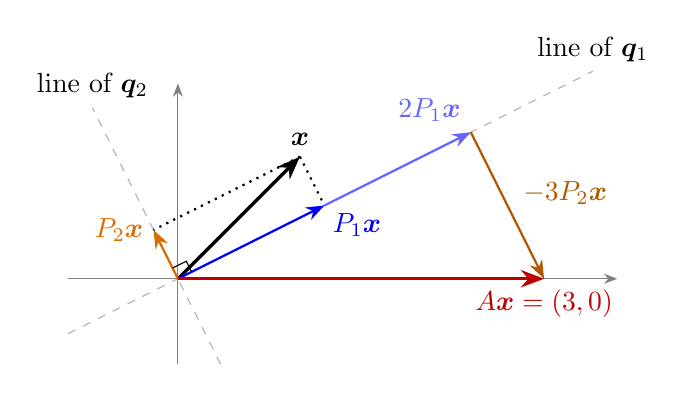
\begin{tikzpicture}[scale=1.55,>=Stealth]
  \draw[gray!60,dashed] (-0.9,-0.45) -- (3.4,1.7) node[above,black] {line of $\vb{q}_1$};
  \draw[gray!60,dashed] (0.35,-0.7) -- (-0.7,1.4) node[above,black] {line of $\vb{q}_2$};
  \draw[->,gray] (-0.9,0) -- (3.6,0);
  \draw[->,gray] (0,-0.7) -- (0,1.6);
  \draw[dotted,thick] (1,1) -- (1.2,0.6);
  \draw[dotted,thick] (1,1) -- (-0.2,0.4);
  \draw[->,very thick] (0,0) -- (1,1) node[above] {$\vb{x}$};
  \draw[->,thick,blue] (0,0) -- (1.2,0.6) node[below right=-1pt] {$P_1\vb{x}$};
  \draw[->,thick,orange!85!black] (0,0) -- (-0.2,0.4) node[left] {$P_2\vb{x}$};
  \draw[->,thick,blue!60] (1.2,0.6) -- (2.4,1.2) node[above left] {$2P_1\vb{x}$};
  \draw[->,thick,orange!70!black] (2.4,1.2) -- (3,0);
  \node[orange!70!black,right] at (2.75,0.7) {$-3P_2\vb{x}$};
  \draw[->,very thick,red!75!black] (0,0) -- (3,0) node[below] {$A\vb{x}=(3,0)$};
  \draw (0.112,0.056) -- (0.068,0.144) -- (-0.044,0.088);
\end{tikzpicture}
\caption{The spectral theorem at work for $A=\left[\begin{smallmatrix}1&2\\2&-2\end{smallmatrix}\right]$
and $\vb{x}=(1,1)$. The eigenvector lines are perpendicular; $\vb{x}$ splits into its projections
$P_1\vb{x}=(1.2,0.6)$ and $P_2\vb{x}=(-0.2,0.4)$; $A$ stretches them by $\lambda_1=2$ and
$\lambda_2=-3$ and adds, giving $A\vb{x}=(3,0)$.}
\label{fig:u29-projections}
\end{figure}

\subsection{Signs of pivots are signs of eigenvalues}

Knowing the eigenvalues are real, the next question is whether they are positive or negative;
for $d\vb{u}/dt=A\vb{u}$ that decides stability (Section~\ref{sec:u25}). Finding the 50
eigenvalues of a $50\times 50$ matrix from $\det(A-\lambda I)=0$ is hopeless: the roots of a
degree-50 polynomial are extremely sensitive to rounding. Pivots, on the other hand, are cheap
and safe to compute. For symmetric matrices they carry the sign information we want.

If elimination on a symmetric $A$ needs no row exchanges, it gives $A=LDU$ with $L$ unit lower
triangular, $D$ the diagonal matrix of pivots and $U$ unit upper triangular
(Section~\ref{sec:u05}). Transposing gives a second such factorization $A=A\T=U\T DL\T$, and
since the $LDU$ factors are unique, $U=L\T$:
\[
  A=LDL\T\qquad (A \text{ symmetric, no row exchanges}).
\]

\begin{theorem}[Pivot signs]\label{thm:u29-signs}
Let $A$ be real symmetric with nonzero pivots $d_1,\dots,d_n$ (no row exchanges). Then the
number of positive pivots equals the number of positive eigenvalues, and likewise for
negative ones.
\end{theorem}
\begin{proof}
Write $A=LDL\T$ and, for $0\le t\le 1$, let $L_t=tL+(1-t)I$. Every $L_t$ is lower triangular with
ones on the diagonal, so $\det L_t=1$. The matrix $A_t=L_tDL_t\T$ is symmetric, so its eigenvalues
are real, and $\det A_t=\det D=d_1\cdots d_n\ne 0$, so $0$ is never an eigenvalue of $A_t$. At
$t=0$, $A_0=D$, whose eigenvalues are the pivots; at $t=1$, $A_1=A$. The eigenvalues of $A_t$ are
the roots of a polynomial whose coefficients depend continuously on $t$, so they move
continuously. A real eigenvalue that changed sign would have to pass through $0$, which never
happens. Hence $A$ and $D$ have the same number of positive eigenvalues.
\end{proof}

The product of the pivots and the product of the eigenvalues are both $\det A$, but that is
one number; the theorem gives $n$ separate pieces of sign information. Combined with a shift
it locates eigenvalues: the eigenvalues of $A-bI$ are $\lambda_k-b$, so the positive pivots of
$A-bI$ count the eigenvalues of $A$ that are larger than $b$.

\begin{example}[Counting eigenvalues above a number]\label{ex:u29-shift}
Let $K=\begin{bmatrix}2&-1&0\\-1&2&-1\\0&-1&2\end{bmatrix}$. How many eigenvalues exceed $5/2$?
Eliminate on
\[
  K-\tfrac52 I=\begin{bmatrix}-\tfrac12&-1&0\\-1&-\tfrac12&-1\\0&-1&-\tfrac12\end{bmatrix}.
\]
The first pivot is $-\tfrac12$. Subtracting $2\times$row~1 from row~2 leaves
$(0,\ \tfrac32,\ -1)$, so the second pivot is $\tfrac32$. Adding $\tfrac23\times$ the new row~2
to row~3 leaves $-\tfrac12-\tfrac23=-\tfrac76$. The pivots $-\tfrac12,\ \tfrac32,\ -\tfrac76$ have one
positive sign, so exactly one eigenvalue of $K$ is above $5/2$. Check: the eigenvalues of $K$
are $2-\sqrt2\approx0.59$, $2$ and $2+\sqrt2\approx3.41$ (Section~\ref{sec:u31}), and only
$2+\sqrt2$ exceeds $2.5$.
\end{example}

\begin{trap}
Pivots are not eigenvalues. For $A=\left[\begin{smallmatrix}5&2\\2&3\end{smallmatrix}\right]$ the
pivots are $5$ and $11/5$, the eigenvalues are $4\pm\sqrt5\approx 6.24,\,1.76$. What they share is
their signs and their product ($\det A=11$). Even the signs agree only for symmetric
matrices: the nonsymmetric $\left[\begin{smallmatrix}1&-6\\1&-4\end{smallmatrix}\right]$ has
positive pivots $1$ and $2$, but its eigenvalues are $-1$ and $-2$.
\end{trap}

\subsection{Positive definite matrices}

\begin{definition}[Positive definite]\label{def:u29-pd}
A \emph{positive definite} matrix is a real symmetric matrix whose eigenvalues are all
positive.
\end{definition}

Symmetric matrices are good; positive definite ones are the best. Testing the definition
directly needs the eigenvalues, but pivots and determinants do the job without them.

\begin{theorem}[Three equivalent tests]\label{thm:u29-pdtests}
For a real symmetric $n\times n$ matrix $A$ the following are equivalent:
\begin{enumerate}[(a)]
  \item all eigenvalues of $A$ are positive;
  \item all $n$ upper-left determinants $D_1=a_{11},\ D_2,\ \dots,\ D_n=\det A$ are positive,
        where $D_k$ is the determinant of the top-left $k\times k$ submatrix $A_k$;
  \item elimination without row exchanges produces $n$ pivots, all positive.
\end{enumerate}
\end{theorem}
\begin{proof}
(a)$\Rightarrow$(b). Write $A=Q\Lambda Q\T$ and $\vb{y}=Q\T\vb{x}$. Then
$\vb{x}\T A\vb{x}=\vb{y}\T\Lambda\vb{y}=\lambda_1y_1^2+\cdots+\lambda_ny_n^2$, which is positive for every
$\vb{x}\ne\vb{0}$ (since then $\vb{y}\ne\vb{0}$). Now take $\vb{z}\in\R^k$, $\vb{z}\ne\vb{0}$, and pad it with
zeros to $\vb{x}=(\vb{z},0,\dots,0)$; then $\vb{z}\T A_k\vb{z}=\vb{x}\T A\vb{x}>0$. If $\mu$ is an eigenvalue of
the symmetric matrix $A_k$ with real eigenvector $\vb{z}$, this says $\mu\,\vb{z}\T\vb{z}>0$, so $\mu>0$.
Hence $D_k=\det A_k$, the product of the eigenvalues of $A_k$, is positive.

(b)$\Rightarrow$(c). Elimination on the first $k$ rows only ever uses entries of $A_k$, so the
first $k$ pivots of $A$ are the pivots of $A_k$ and $D_k=d_1d_2\cdots d_k$. If every $D_k>0$, then
$d_1=D_1>0$ and $d_k=D_k/D_{k-1}>0$; in particular no zero pivot forces a row exchange.

(c)$\Rightarrow$(a). With all pivots positive, Theorem~\ref{thm:u29-signs} says all $n$
eigenvalues are positive.
\end{proof}

The quantity $\vb{x}\T A\vb{x}$ that appeared in the first step will become the central character
of Section~\ref{sec:u31}, where it gives a fourth test and the link to minima.

\begin{example}[The lecture's example]\label{ex:u29-532}
$A=\begin{bmatrix}5&2\\2&3\end{bmatrix}$ is symmetric. Its upper-left determinants are $5$ and
$15-4=11$, both positive. Its pivots are $5$ and $11/5$ (the second pivot is $\det A$ divided by
the first). So $A$ is positive definite, and the eigenvalues must be positive without our
computing them. Computing anyway: $\lambda^2-8\lambda+11=0$ gives $\lambda=4\pm\sqrt{16-11}=4\pm\sqrt5$,
and $4-\sqrt5\approx1.76>0$.

By contrast $B=\begin{bmatrix}-1&0\\0&-3\end{bmatrix}$ has $\det B=3>0$, yet its eigenvalues
(and pivots) are $-1$ and $-3$. It fails test~(b) at the first step: $D_1=-1<0$.
\end{example}

\begin{trap}
A positive determinant does not make a symmetric matrix positive definite: two negative
eigenvalues also multiply to a positive number. Test \emph{all} $n$ upper-left determinants,
not only the last one. Another quick necessary condition: every diagonal entry
$a_{ii}=\vb{e}_i\T A\vb{e}_i$ of a positive definite matrix is positive, so a single
$a_{ii}\le0$ rules it out at once.
\end{trap}

Some immediate consequences, each read off from the eigenvalues:
\begin{itemize}
  \item a positive definite matrix is invertible, since $\det A=\lambda_1\cdots\lambda_n>0$;
  \item a diagonal matrix with positive diagonal entries is positive definite, since those entries
        are its eigenvalues;
  \item the inverse of a positive definite matrix is positive definite, with eigenvalues
        $1/\lambda_k>0$ (more of this in Section~\ref{sec:u32}).
\end{itemize}

\subsection{Exercises}

\begin{exercise}[Where a false proof breaks]\label{exr:u29-false}
Here is a ``proof'' that every real matrix has real eigenvalues: from $A\vb{x}=\lambda\vb{x}$ we get
$\vb{x}\T A\vb{x}=\lambda\,\vb{x}\T\vb{x}$, so $\lambda=\vb{x}\T A\vb{x}/\vb{x}\T\vb{x}$, a ratio of real numbers.
Test each step on the rotation $A=\left[\begin{smallmatrix}0&-1\\1&0\end{smallmatrix}\right]$ with
$\lambda=i$ and $\vb{x}=(i,1)$, and find the hidden assumption.
\end{exercise}
\begin{solution}
First $A\vb{x}=(0\cdot i-1,\ i+0)=(-1,\,i)=i\,(i,1)$, so $\lambda=i$ really is an eigenvalue. Next,
$\vb{x}\T A\vb{x}=(i,1)\cdot(-1,i)=-i+i=0$ and $\lambda\,\vb{x}\T\vb{x}=i\,(i^2+1)=0$, so the equation
$\vb{x}\T A\vb{x}=\lambda\vb{x}\T\vb{x}$ holds, as $0=0$. The final step divides by $\vb{x}\T\vb{x}=i^2+1^2=0$.
The hidden assumption is $\vb{x}\T\vb{x}\ne0$, which is true for real vectors but false for complex
ones; and the ratio is not obviously real either, since $\vb{x}$ may be complex. The correct
version uses $\bar{\vb{x}}\T\vb{x}=|x_1|^2+|x_2|^2>0$ (Lemma~\ref{lem:u29-xbarx}) and needs symmetry.
\end{solution}

\begin{exercise}[Which families are groups?]\label{exr:u29-groups}
A family of invertible matrices is a \emph{group} if it contains $AB$ and $A^{-1}$ whenever it
contains $A$ and $B$. Which of these are groups?
\begin{enumerate}[(a)]
  \item symmetric positive definite matrices;
  \item orthogonal matrices;
  \item all exponentials $e^{tA}$ of one fixed matrix $A$, $t\in\R$;
  \item matrices with determinant~1.
\end{enumerate}
\end{exercise}
\begin{solution}
\begin{enumerate}[(a)]
  \item No. $A=\left[\begin{smallmatrix}2&1\\1&1\end{smallmatrix}\right]$ (upper-left determinants $2,1$) and
        $B=\left[\begin{smallmatrix}1&1/2\\1/2&1\end{smallmatrix}\right]$ (determinants $1,3/4$) are positive
        definite, but $AB=\left[\begin{smallmatrix}2.5&2\\1.5&1.5\end{smallmatrix}\right]$ is not even
        symmetric. (Inverses do stay positive definite.)
  \item Yes. If $A\T A=I$ then $A^{-1}=A\T$ and $(A\T)\T A\T=AA\T=I$; if also $B\T B=I$ then
        $(AB)\T(AB)=B\T A\T AB=B\T B=I$.
  \item Yes. $(e^{pA})^{-1}=e^{-pA}$ and $e^{pA}e^{qA}=e^{(p+q)A}$ are again of the form $e^{tA}$.
  \item Yes. $\det(A^{-1})=1/\det A=1$ and $\det(AB)=\det A\det B=1$.
\end{enumerate}
\end{solution}

\begin{exercise}[Projections and determinants]\label{exr:u29-projection}
\begin{enumerate}[(a)]
  \item Show that the only positive definite projection matrix is $P=I$.
  \item Show that $S=\left[\begin{smallmatrix}-3&1\\1&-2\end{smallmatrix}\right]$ has $\det S>0$ but is not
        positive definite, by exhibiting $\vb{x}$ with $\vb{x}\T S\vb{x}<0$.
\end{enumerate}
\end{exercise}
\begin{solution}
\begin{enumerate}[(a)]
  \item A projection satisfies $P^2=P$, so each eigenvalue satisfies $\lambda^2=\lambda$: $\lambda\in\{0,1\}$.
        Positive definite forces $\lambda>0$, so all eigenvalues are $1$. A projection matrix is
        symmetric, so $P=Q\Lambda Q\T=QIQ\T=I$.
  \item $\det S=6-1=5>0$, but $\vb{x}=(1,0)$ gives $\vb{x}\T S\vb{x}=s_{11}=-3<0$. In the language of
        Theorem~\ref{thm:u29-pdtests}, $D_1=-3$ fails. In fact both eigenvalues,
        $(-5\pm\sqrt5)/2\approx-1.38,\,-3.62$, are negative: $S$ is negative definite.
\end{enumerate}
\end{solution}

\begin{exercise}[Spectral decomposition and pivots]\label{exr:u29-345}
For $A=\left[\begin{smallmatrix}3&4\\4&-3\end{smallmatrix}\right]$ find $\lambda_1,\lambda_2$, write
$A=\lambda_1P_1+\lambda_2P_2$ with projections $P_k=\vb{q}_k\vb{q}_k\T$, and confirm that the pivot signs
match the eigenvalue signs.
\end{exercise}
\begin{solution}
Trace $0$ and determinant $-9-16=-25$ give $\lambda^2-25=0$, so $\lambda=\pm5$. From
$A-5I=\left[\begin{smallmatrix}-2&4\\4&-8\end{smallmatrix}\right]$ the eigenvector is $(2,1)$; from
$A+5I=\left[\begin{smallmatrix}8&4\\4&2\end{smallmatrix}\right]$ it is $(1,-2)$; they are perpendicular.
With $\vb{q}_1=(2,1)/\sqrt5$, $\vb{q}_2=(1,-2)/\sqrt5$,
\[
  5\cdot\tfrac15\begin{bmatrix}4&2\\2&1\end{bmatrix}-5\cdot\tfrac15\begin{bmatrix}1&-2\\-2&4\end{bmatrix}
  =\begin{bmatrix}3&4\\4&-3\end{bmatrix}.
\]
Elimination subtracts $\tfrac43$ of row~1 from row~2, so the pivots are $3$ and
$-3-\tfrac{16}{3}=-\tfrac{25}{3}$: one positive, one negative, like $5$ and $-5$. Their product is
$-25=\det A$.
\end{solution}

% unit: u30
% sources: sources/075-complex-matrices-fast-fourier-transform-fft.txt, sources/051-lecture-26-complex-matrices-fast-fourier-transform-fft.txt, sources/209-mit18-06scf11-ses3-2sum-pdf-download-file.txt, sources/052-problem-solving-complex-matrices.txt, sources/210-mit18-06scf11-ses3-2prob-pdf-download-file.txt, sources/211-mit18-06scf11-ses3-2sol-pdf-download-file.txt
\providecommand{\Hm}{^{\mathsf{H}}}% conjugate transpose: A\Hm
\section{Complex matrices; fast Fourier transform (FFT)}\label{sec:u30}

Complex numbers have slipped into the course through the back door: a real matrix such as a
rotation can have complex eigenvalues and eigenvectors. This unit says once and for all what
changes when vectors and matrices are complex. Only one rule is new: \emph{whenever we
transpose, we also take complex conjugates}. With that rule, symmetric matrices become
Hermitian matrices and orthogonal matrices become unitary ones.

The payoff is the most important complex matrix of all, the Fourier matrix $F_n$. It has
orthogonal columns, so it is easy to invert, and it has so much structure that it can be
multiplied by a vector in about $\tfrac12 n\log_2 n$ steps instead of $n^2$. That algorithm, the
fast Fourier transform, is a matrix factorization, and it changed scientific computing.

\subsection{Length and inner product in \texorpdfstring{$\C^n$}{C\^{}n}}

A vector $\vb{z}=(z_1,\dots,z_n)$ with complex components lives in $\C^n$. The old length formula
$\vb{z}\T\vb{z}=z_1^2+\cdots+z_n^2$ is no good: for $\vb{z}=(1,i)$ it gives $1+i^2=0$, so a nonzero vector
would have length zero. The cure is to conjugate one factor, because $\bar z z=|z|^2\ge0$
(Section~\ref{sec:u29}).

\begin{definition}[Conjugate transpose, length, inner product]\label{def:u30-hermitian-transpose}
For a complex matrix or vector, $A\Hm=\bar A\T$ is the \emph{conjugate transpose} (read
``$A$ Hermitian''; the $\mathsf{H}$ honours Charles Hermite). For $\vb{z},\vb{x},\vb{y}\in\C^n$,
\[
  \|\vb{z}\|^2=\vb{z}\Hm\vb{z}=|z_1|^2+\cdots+|z_n|^2,
  \qquad
  \vb{y}\Hm\vb{x}=\bar y_1x_1+\cdots+\bar y_nx_n .
\]
The vectors $\vb{x}$ and $\vb{y}$ are \emph{orthogonal} when $\vb{y}\Hm\vb{x}=0$.
\end{definition}

The inner product $\vb{y}\Hm\vb{x}$ is usually a complex number; only $\vb{z}\Hm\vb{z}$ is guaranteed real
and nonnegative. The definition is forced on us: the inner product of a vector with itself
must be its length squared.

\begin{proposition}[Rules for \texorpdfstring{$\mathsf{H}$}{H}]\label{prop:u30-rules}
For complex vectors and matrices of compatible sizes:
(a) $\vb{x}\Hm\vb{y}=\overline{\vb{y}\Hm\vb{x}}$;
(b) $(AB)\Hm=B\Hm A\Hm$;
(c) $(A\vb{x})\Hm\vb{y}=\vb{x}\Hm(A\Hm\vb{y})$.
\end{proposition}
\begin{proof}
(a) $\overline{\sum\bar y_kx_k}=\sum y_k\bar x_k=\vb{x}\Hm\vb{y}$.
(b) Conjugation respects products, $\overline{AB}=\bar A\bar B$, and transposing reverses the
order: $(\bar A\bar B)\T=\bar B\T\bar A\T$.
(c) By (b), $(A\vb{x})\Hm=\vb{x}\Hm A\Hm$.
\end{proof}

\begin{example}[Lengths and right angles in \texorpdfstring{$\C^2$}{C\^{}2}]\label{ex:u30-c2}
For $\vb{z}=(1,i)$: $\vb{z}\Hm\vb{z}=\bar1\cdot1+\bar i\cdot i=1+(-i)(i)=2$, so $\|\vb{z}\|=\sqrt2$, not $0$.
For $\vb{x}=(1,i)$ and $\vb{y}=(i,1)$: $\vb{y}\Hm\vb{x}=\bar i\cdot1+\bar1\cdot i=-i+i=0$. These two vectors
are orthogonal in $\C^2$, even though the unconjugated product $\vb{y}\T\vb{x}=i+i=2i$ is not zero.
\end{example}

\subsection{Hermitian matrices}

\begin{definition}[Hermitian matrix]\label{def:u30-hermitian}
A square complex matrix is \emph{Hermitian} if $A\Hm=A$, that is $a_{ji}=\bar a_{ij}$ for all
$i,j$. In particular each diagonal entry equals its own conjugate, so it is real.
\end{definition}

For example $\begin{bmatrix}2&3+i\\3-i&5\end{bmatrix}$ is Hermitian: flipping across the
diagonal and conjugating returns the same matrix. A real matrix is Hermitian exactly when it is
symmetric, so everything below includes Section~\ref{sec:u29} as a special case.

\begin{theorem}[Hermitian matrices are as good as symmetric ones]\label{thm:u30-hermitian}
Let $A\Hm=A$. Then
\begin{enumerate}[(a)]
  \item $\vb{z}\Hm A\vb{z}$ is real for every $\vb{z}\in\C^n$;
  \item every eigenvalue of $A$ is real;
  \item eigenvectors for different eigenvalues are orthogonal: $\vb{y}\Hm\vb{x}=0$.
\end{enumerate}
\end{theorem}
\begin{proof}
(a) The number $\vb{z}\Hm A\vb{z}$ is a $1\times1$ matrix, so it equals its transpose, and its
conjugate is $(\vb{z}\Hm A\vb{z})\Hm=\vb{z}\Hm A\Hm\vb{z}=\vb{z}\Hm A\vb{z}$. A number equal to its conjugate
is real.
(b) If $A\vb{x}=\lambda\vb{x}$ with $\vb{x}\ne\vb{0}$, then $\vb{x}\Hm A\vb{x}=\lambda\,\vb{x}\Hm\vb{x}$. The left side
is real by (a) and $\vb{x}\Hm\vb{x}>0$ is real, so $\lambda$ is real.
(c) Let $A\vb{x}=\lambda\vb{x}$, $A\vb{y}=\mu\vb{y}$, $\lambda\ne\mu$, both real by (b). Then
$\vb{y}\Hm A\vb{x}=\lambda\,\vb{y}\Hm\vb{x}$, and also
$\vb{y}\Hm A\vb{x}=(A\Hm\vb{y})\Hm\vb{x}=(A\vb{y})\Hm\vb{x}=\bar\mu\,\vb{y}\Hm\vb{x}=\mu\,\vb{y}\Hm\vb{x}$.
Subtracting, $(\lambda-\mu)\vb{y}\Hm\vb{x}=0$, so $\vb{y}\Hm\vb{x}=0$.
\end{proof}

The proof of the spectral theorem in Section~\ref{sec:u29} goes through word for word
with $\mathsf{T}$ replaced by $\mathsf{H}$: every Hermitian matrix is $A=U\Lambda U\Hm$ with $\Lambda$
real and $U$ unitary (defined next).

\begin{example}[Diagonalizing a Hermitian matrix]\label{ex:u30-diag}
Let $A=\begin{bmatrix}2&1-i\\1+i&3\end{bmatrix}$. It is Hermitian: the diagonal is real and the
off-diagonal entries are conjugates.

\emph{Eigenvalues.}
$\det(A-\lambda I)=(2-\lambda)(3-\lambda)-(1-i)(1+i)=\lambda^2-5\lambda+6-2=\lambda^2-5\lambda+4$,
because $(1-i)(1+i)=1-i^2=2$. So $(\lambda-1)(\lambda-4)=0$: $\lambda_1=1$, $\lambda_2=4$, real although
$A$ is complex.

\emph{Eigenvectors.} For $\lambda=1$, $A-I=\left[\begin{smallmatrix}1&1-i\\1+i&2\end{smallmatrix}\right]$.
The second row is $(1+i)$ times the first, because $(1+i)(1-i)=2$; the rows are dependent, as
they must be. The first row is solved by $\vb{v}=(1-i,\,-1)$: $1\cdot(1-i)+(1-i)(-1)=0$. For
$\lambda=4$, $A-4I=\left[\begin{smallmatrix}-2&1-i\\1+i&-1\end{smallmatrix}\right]$; the second row
gives $\vb{u}=(1,\,1+i)$. Check: $A\vb{u}=(2+(1-i)(1+i),\ 1+i+3(1+i))=(4,\,4+4i)=4\vb{u}$.

\emph{Orthogonality.} $\vb{v}\Hm\vb{u}=\overline{(1-i)}\cdot1+\overline{(-1)}(1+i)=(1+i)-(1+i)=0$.

\emph{Unitary eigenvector matrix.} Both vectors have length $\sqrt3$: $|1-i|^2+|{-1}|^2=2+1$ and
$1+|1+i|^2=1+2$. Dividing by $\sqrt3$,
\[
  A=U\Lambda U\Hm=\frac{1}{\sqrt3}\begin{bmatrix}1-i&1\\-1&1+i\end{bmatrix}
  \begin{bmatrix}1&0\\0&4\end{bmatrix}
  \frac{1}{\sqrt3}\begin{bmatrix}1+i&-1\\1&1-i\end{bmatrix}.
\]
Multiplying out: the $(1,1)$ entry is $\tfrac13\bigl[(1-i)(1+i)+4\bigr]=\tfrac13(2+4)=2$, the $(1,2)$
entry is $\tfrac13\bigl[-(1-i)+4(1-i)\bigr]=1-i$, and similarly for the rest, recovering $A$.
\end{example}

\begin{trap}
A complex matrix that is merely \emph{symmetric} has none of these properties.
$\left[\begin{smallmatrix}1&i\\i&1\end{smallmatrix}\right]$ equals its transpose but not its
conjugate transpose, and its eigenvalues $1\pm i$ (eigenvectors $(1,1)$ and $(1,-1)$) are not real.
For complex matrices, check $A\Hm=A$, never only $A\T=A$.
\end{trap}

\subsection{Unitary matrices}

\begin{definition}[Unitary matrix]\label{def:u30-unitary}
A square complex matrix $U$ is \emph{unitary} if $U\Hm U=I$: its columns are orthonormal in the
sense $\vb{u}_j\Hm\vb{u}_k=0$ for $j\ne k$ and $\vb{u}_k\Hm\vb{u}_k=1$. Then $U^{-1}=U\Hm$.
\end{definition}

\begin{proposition}[Unitary matrices preserve lengths]\label{prop:u30-unitary}
If $U$ is unitary then $(U\vb{x})\Hm(U\vb{y})=\vb{x}\Hm\vb{y}$ and $\|U\vb{z}\|=\|\vb{z}\|$ for all vectors, and
every eigenvalue of $U$ has $|\lambda|=1$.
\end{proposition}
\begin{proof}
$(U\vb{x})\Hm(U\vb{y})=\vb{x}\Hm U\Hm U\vb{y}=\vb{x}\Hm\vb{y}$; take $\vb{x}=\vb{y}=\vb{z}$ for lengths. If
$U\vb{z}=\lambda\vb{z}$ with $\vb{z}\ne\vb{0}$, then $\|\vb{z}\|=\|U\vb{z}\|=|\lambda|\,\|\vb{z}\|$, so $|\lambda|=1$.
\end{proof}

The translation from real to complex is mechanical; Table~\ref{tab:u30-dictionary} collects it.

\begin{table}[ht]\centering
\begin{tabular}{@{}lll@{}}
\toprule
 & real ($\R^n$) & complex ($\C^n$) \\
\midrule
length squared & $\vb{x}\T\vb{x}=\sum x_k^2$ & $\vb{z}\Hm\vb{z}=\sum |z_k|^2$ \\
inner product & $\vb{y}\T\vb{x}$ & $\vb{y}\Hm\vb{x}$ \\
transpose rule & $(AB)\T=B\T A\T$ & $(AB)\Hm=B\Hm A\Hm$ \\
good matrices & symmetric, $A\T=A$ & Hermitian, $A\Hm=A$ \\
orthonormal columns & orthogonal, $Q\T Q=I$ & unitary, $U\Hm U=I$ \\
spectral theorem & $A=Q\Lambda Q\T$ & $A=U\Lambda U\Hm$ \\
\bottomrule
\end{tabular}
\caption{The dictionary between $\R^n$ and $\C^n$: transpose becomes conjugate transpose.}
\label{tab:u30-dictionary}
\end{table}

\subsection{The Fourier matrix}

Electrical engineers number rows and columns from $0$ to $n-1$, and for the Fourier matrix we
follow them.

\begin{definition}[Fourier matrix]\label{def:u30-fourier}
Let $w=w_n=e^{2\pi i/n}=\cos\frac{2\pi}{n}+i\sin\frac{2\pi}{n}$. The $n\times n$ \emph{Fourier matrix}
$F_n$ has entries $(F_n)_{jk}=w^{jk}$ for $j,k=0,1,\dots,n-1$:
\[
  F_n=\begin{bmatrix}
  1&1&1&\cdots&1\\
  1&w&w^2&\cdots&w^{n-1}\\
  1&w^2&w^4&\cdots&w^{2(n-1)}\\
  \vdots&\vdots&\vdots&&\vdots\\
  1&w^{n-1}&w^{2(n-1)}&\cdots&w^{(n-1)^2}
  \end{bmatrix}.
\]
\end{definition}

The number $w$ sits on the unit circle at angle $2\pi/n$, one $n$th of the way round, and
$w^n=1$. Its powers $1,w,w^2,\dots,w^{n-1}$ are the $n$ different $n$th roots of $1$, equally
spaced on the circle (Figure~\ref{fig:u30-roots}). Powers are easy in the polar form:
$w^{k}=e^{2\pi ik/n}$, which is why we never expand $w$ into cosines and sines. Note that
$F_n\T=F_n$ (symmetric in the old sense), but $F_n$ is not Hermitian.

\begin{figure}[ht]\centering
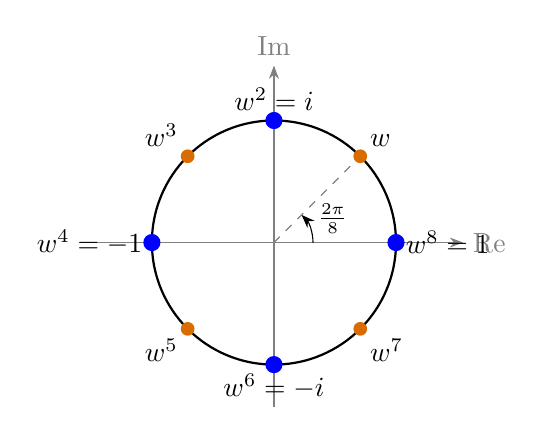
\begin{tikzpicture}[scale=1.55,>=Stealth]
  \draw[->,gray] (-1.45,0) -- (1.55,0) node[right] {$\mathrm{Re}$};
  \draw[->,gray] (0,-1.35) -- (0,1.45) node[above] {$\mathrm{Im}$};
  \draw[thick] (0,0) circle (1);
  \draw[->] (0.32,0) arc (0:45:0.32);
  \node at (22:0.52) {\small $\tfrac{2\pi}{8}$};
  \draw[dashed,gray] (0,0) -- (45:1);
  \foreach \k in {1,3,5,7} {
    \fill[orange!85!black] (45*\k:1) circle (1.6pt);
  }
  \foreach \k in {2,4,6,8} {
    \fill[blue] (45*\k:1) circle (2.0pt);
  }
  \node[above right] at (45:1) {$w$};
  \node[above] at (90:1) {$w^2=i$};
  \node[above left] at (135:1) {$w^3$};
  \node[left] at (180:1) {$w^4=-1$};
  \node[below left] at (225:1) {$w^5$};
  \node[below] at (270:1) {$w^6=-i$};
  \node[below right] at (315:1) {$w^7$};
  \node[right] at (0:1) {$w^8=1$};
\end{tikzpicture}
\caption{The eighth roots of unity, powers of $w=w_8=e^{2\pi i/8}$. The even powers (blue)
$w^2,w^4,w^6,w^8$ are exactly the fourth roots of unity $i,-1,-i,1$: squaring $w_8$ gives $w_4$.
This doubling of angles is what links $F_8$ to $F_4$ in the FFT.}
\label{fig:u30-roots}
\end{figure}

For $n=4$, $w=e^{2\pi i/4}=i$ and the exponent is always (row number)$\times$(column number):
\[
  F_4=\begin{bmatrix}1&1&1&1\\1&i&i^2&i^3\\1&i^2&i^4&i^6\\1&i^3&i^6&i^9\end{bmatrix}
     =\begin{bmatrix}1&1&1&1\\1&i&-1&-i\\1&-1&1&-1\\1&-i&-1&i\end{bmatrix}.
\]
Multiplying a four-component signal by $F_4$ (or by $F_4^{-1}$) is the four-point discrete Fourier
transform.

\begin{theorem}[The columns of \texorpdfstring{$F_n$}{F\_n} are orthogonal]\label{thm:u30-orth}
$F_n\Hm F_n=nI$. Hence $\frac{1}{\sqrt n}F_n$ is unitary and
\[
  F_n^{-1}=\frac1n F_n\Hm=\frac1n\bar F_n .
\]
\end{theorem}
\begin{proof}
The $(k,l)$ entry of $F_n\Hm F_n$ is the inner product of columns $k$ and $l$:
\[
  \sum_{j=0}^{n-1}\overline{w^{jk}}\,w^{jl}=\sum_{j=0}^{n-1}w^{j(l-k)}=\sum_{j=0}^{n-1}r^j,
  \qquad r=w^{l-k},
\]
using $\bar w=w^{-1}$ (because $|w|=1$). If $k=l$ then $r=1$ and the sum is $n$. If $k\ne l$
then $0<|l-k|<n$, so $r\ne1$, while $r^n=(w^n)^{l-k}=1$; the geometric series gives
$\sum_{j=0}^{n-1}r^j=(1-r^n)/(1-r)=0$. The last equality uses $F_n\T=F_n$, so
$F_n\Hm=\bar F_n$.
\end{proof}

\begin{example}[Orthogonality and an impulse]\label{ex:u30-f4}
Columns $1$ and $3$ of $F_4$ are $(1,i,-1,-i)$ and $(1,-i,-1,i)$. Without conjugating, their
product is $1+1+1+1=4$, which looks far from orthogonal. With the conjugate,
$\overline{(1,i,-1,-i)}\cdot(1,-i,-1,i)=1\cdot1+(-i)(-i)+(-1)(-1)+(i)(i)=1-1+1-1=0$.

The impulse $\vb{x}=(1,0,0,0)$ transforms to $F_4\vb{x}=(1,1,1,1)$, the first column: a single
impulse contains all frequencies in equal amounts. Transforming back with
$F_4^{-1}=\tfrac14\bar F_4$ gives $\tfrac14(1+1+1+1,\ 1-i-1+i,\ 0,\ 0)=(1,0,0,0)$.
\end{example}

\begin{trap}
The inverse of $F_n$ is $\frac1n\bar F_n$, not $\frac1nF_n$. For the impulse above both happen to
give the same answer, but in general $F_4F_4=4\left[\begin{smallmatrix}1&0&0&0\\0&0&0&1\\0&0&1&0\\0&1&0&0\end{smallmatrix}\right]$:
applying $F_4$ twice reverses components $1,2,3$ of the signal instead of restoring it.
\end{trap}

\subsection{The fast Fourier transform}

Multiplying $F_n\vb{x}$ directly needs $n^2$ multiplications, since $F_n$ has no zero entries.
The fast Fourier transform (FFT) connects $F_{2m}$ to two copies of $F_m$, using the fact seen in
Figure~\ref{fig:u30-roots}:
\[
  w_{2m}^2=\bigl(e^{2\pi i/2m}\bigr)^2=e^{2\pi i/m}=w_m ,
  \qquad
  w_{2m}^m=e^{\pi i}=-1 .
\]

\begin{theorem}[FFT factorization]\label{thm:u30-fft}
Let $D=\operatorname{diag}(1,w,w^2,\dots,w^{m-1})$ with $w=w_{2m}$, and let $P$ be the
$2m\times 2m$ permutation matrix that puts the even-numbered components first,
\[
  P(x_0,x_1,\dots,x_{2m-1})=(x_0,x_2,\dots,x_{2m-2},\ x_1,x_3,\dots,x_{2m-1}).
\]
Then
\[
  F_{2m}=\begin{bmatrix}I&D\\I&-D\end{bmatrix}\begin{bmatrix}F_m&0\\0&F_m\end{bmatrix}P .
\]
\end{theorem}
\begin{proof}
Let $\vb{y}=F_{2m}\vb{x}$ and split the sum $y_j=\sum_{k=0}^{2m-1}w_{2m}^{jk}x_k$ into even $k=2l$ and
odd $k=2l+1$:
\[
  y_j=\sum_{l=0}^{m-1}w_{2m}^{2jl}x_{2l}+w_{2m}^{j}\sum_{l=0}^{m-1}w_{2m}^{2jl}x_{2l+1}
     =y'_j+w_{2m}^{\,j}\,y''_j ,
\]
where $\vb{y}'=F_m(x_0,x_2,\dots)$ and $\vb{y}''=F_m(x_1,x_3,\dots)$, because $w_{2m}^{2jl}=w_m^{jl}$. For
$0\le j<m$ this is the top half of the right side. For the bottom half, replace $j$ by $j+m$:
$w_m^{(j+m)l}=w_m^{jl}$ (as $w_m^m=1$), so $\vb{y}'$ and $\vb{y}''$ are unchanged, while
$w_{2m}^{j+m}=-w_{2m}^j$. Hence $y_{j+m}=y'_j-w_{2m}^jy''_j$, which is the bottom half.
\end{proof}

In words: separate $\vb{x}$ into evens and odds (free), do two half-size transforms, then
recombine with $m$ multiplications by the entries of $D$ and $2m$ additions.

\begin{figure}[ht]\centering
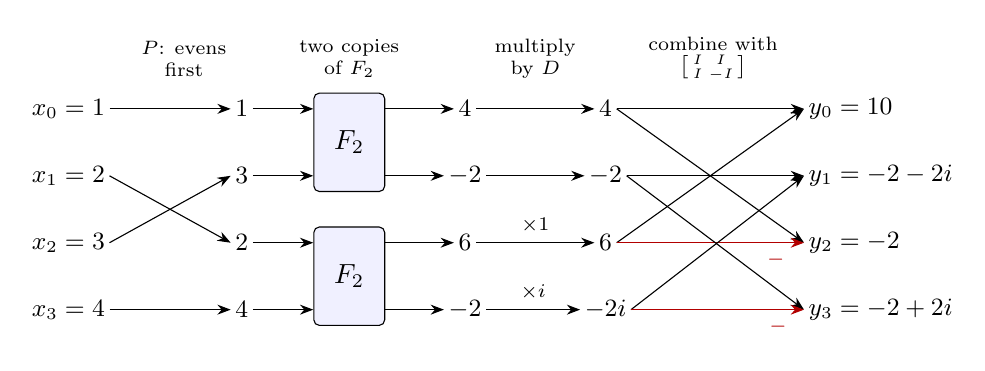
\begin{tikzpicture}[>=Stealth,x=1.05cm,y=0.85cm,
  val/.style={font=\small,inner sep=1.5pt},
  box/.style={draw,rounded corners=2pt,fill=blue!6,minimum width=0.9cm,minimum height=1.25cm}]
  \foreach \r/\lab in {0/{x_0=1},1/{x_1=2},2/{x_2=3},3/{x_3=4}}
    \node[val,anchor=east] (in\r) at (0,-\r) {$\lab$};
  \foreach \r/\lab in {0/1,1/3,2/2,3/4}
    \node[val] (p\r) at (1.6,-\r) {$\lab$};
  \draw[->] (in0.east) -- (p0.west);
  \draw[->] (in2.east) -- (p1.west);
  \draw[->] (in1.east) -- (p2.west);
  \draw[->] (in3.east) -- (p3.west);
  \node[box] (fa) at (2.9,-0.5) {$F_2$};
  \node[box] (fb) at (2.9,-2.5) {$F_2$};
  \foreach \r/\b in {0/fa,1/fa,2/fb,3/fb} \draw[->] (p\r.east) -- (\b.west |- p\r);
  \foreach \r/\lab in {0/4,1/{-2},2/6,3/{-2}}
    \node[val] (q\r) at (4.3,-\r) {$\lab$};
  \foreach \r/\b in {0/fa,1/fa,2/fb,3/fb} \draw[->] (\b.east |- q\r) -- (q\r.west);
  \foreach \r/\lab in {0/4,1/{-2},2/6,3/{-2i}}
    \node[val] (d\r) at (6.0,-\r) {$\lab$};
  \draw[->] (q0) -- (d0); \draw[->] (q1) -- (d1);
  \draw[->] (q2) -- node[above,font=\scriptsize] {$\times1$} (d2);
  \draw[->] (q3) -- node[above,font=\scriptsize] {$\times i$} (d3);
  \foreach \r/\lab in {0/10,1/{-2-2i},2/{-2},3/{-2+2i}}
    \node[val,anchor=west] (y\r) at (8.4,-\r) {$y_{\r}=\lab$};
  \draw[->] (d0.east) -- (y0.west);
  \draw[->] (d0.east) -- (y2.west);
  \draw[->] (d2.east) -- (y0.west);
  \draw[->,red!70!black] (d2.east) -- node[pos=0.85,below,font=\scriptsize] {$-$} (y2.west);
  \draw[->] (d1.east) -- (y1.west);
  \draw[->] (d1.east) -- (y3.west);
  \draw[->] (d3.east) -- (y1.west);
  \draw[->,red!70!black] (d3.east) -- node[pos=0.85,below,font=\scriptsize] {$-$} (y3.west);
  \node[font=\scriptsize,align=center] at (0.9,0.75) {$P$: evens\\first};
  \node[font=\scriptsize,align=center] at (2.9,0.75) {two copies\\of $F_2$};
  \node[font=\scriptsize,align=center] at (5.15,0.75) {multiply\\by $D$};
  \node[font=\scriptsize,align=center] at (7.3,0.75) {combine with\\$\left[\begin{smallmatrix}I&I\\I&-I\end{smallmatrix}\right]$};
\end{tikzpicture}
\caption{The factorization $F_4=\left[\begin{smallmatrix}I&D\\I&-D\end{smallmatrix}\right]
\left[\begin{smallmatrix}F_2&0\\0&F_2\end{smallmatrix}\right]P$ applied to $\vb{x}=(1,2,3,4)$. Each
``butterfly'' on the right forms a sum and a difference (red lines carry the minus sign). Only the
twiddle step $\times i$ costs a genuine multiplication.}
\label{fig:u30-butterfly}
\end{figure}

\begin{example}[A four-point FFT, step by step]\label{ex:u30-fft4}
For $F_4$ we have $m=2$, $w_4=i$, $D=\operatorname{diag}(1,i)$ and $F_2=\left[\begin{smallmatrix}1&1\\1&-1\end{smallmatrix}\right]$.
Take $\vb{x}=(1,2,3,4)$.
\begin{enumerate}
  \item Permute: evens $(x_0,x_2)=(1,3)$, odds $(x_1,x_3)=(2,4)$.
  \item Half-size transforms: $\vb{y}'=F_2(1,3)=(4,-2)$ and $\vb{y}''=F_2(2,4)=(6,-2)$.
  \item Twiddle: $D\vb{y}''=(1\cdot6,\ i\cdot(-2))=(6,-2i)$.
  \item Combine: top $\vb{y}'+D\vb{y}''=(10,\,-2-2i)$, bottom $\vb{y}'-D\vb{y}''=(-2,\,-2+2i)$.
\end{enumerate}
So $F_4\vb{x}=(10,\,-2-2i,\,-2,\,-2+2i)$. Directly from the rows of $F_4$:
$1+2+3+4=10$; $1+2i-3-4i=-2-2i$; $1-2+3-4=-2$; $1-2i-3+4i=-2+2i$. The two agree.
Figure~\ref{fig:u30-butterfly} shows the same computation as a flow diagram.
\end{example}

\begin{proposition}[Operation count]\label{prop:u30-count}
For $n=2^\ell$, applying Theorem~\ref{thm:u30-fft} recursively computes $F_n\vb{x}$ with
$\tfrac12 n\log_2 n$ multiplications (counting the multiplications by entries of $D$).
\end{proposition}
\begin{proof}
Let $C(n)$ be the count. A size-$n$ transform costs two size-$n/2$ transforms plus $n/2$
multiplications by $D$, so $C(n)=2C(n/2)+\tfrac n2$ with $C(1)=0$. If $C(n/2)=\tfrac12\cdot\tfrac n2(\ell-1)$,
then $C(n)=\tfrac n2(\ell-1)+\tfrac n2=\tfrac n2\ell$, and induction on $\ell$ finishes the proof.
\end{proof}

Unrolling the recursion explains the count: there are $\log_2 n$ levels (for $n=64$: $64\to32\to16\to8\to4\to2\to1$,
six levels), each level's fix-up costs $n/2$ multiplications, and the permutations at all
levels together just reorder the input (evens of evens, evens of odds, and so on). For
$n=1024=2^{10}$, direct multiplication costs $1024^2\approx 10^6$, while the FFT costs
$\tfrac12\cdot1024\cdot10=5120$, about $200$ times less. Since $F_n^{-1}=\frac1n\bar F_n$, the inverse
transform runs through the same algorithm with $\bar w$ in place of $w$. All of this rests on
$F_n$ being a very special matrix with orthogonal columns.

\subsection{Exercises}

\begin{exercise}[The smallest Fourier matrix]\label{exr:u30-f2}
Compute $F_2$, check that $F_2\Hm F_2=2I$, and explain why $F_2^{-1}=\frac12F_2$ even though
$F_n^{-1}\ne\frac1nF_n$ in general.
\end{exercise}
\begin{solution}
For $n=2$, $w=e^{2\pi i/2}=e^{\pi i}=-1$, so $F_2=\left[\begin{smallmatrix}1&1\\1&w\end{smallmatrix}\right]
=\left[\begin{smallmatrix}1&1\\1&-1\end{smallmatrix}\right]$. It is real and symmetric, so
$F_2\Hm F_2=F_2^2=\left[\begin{smallmatrix}2&0\\0&2\end{smallmatrix}\right]=2I$. In general
$F_n^{-1}=\frac1n\bar F_n$; here $\bar F_2=F_2$ because all entries are real, so the two formulas
coincide.
\end{solution}

\begin{exercise}[One step of the FFT for \texorpdfstring{$n=8$}{n = 8}]\label{exr:u30-f8}
In $F_8=\left[\begin{smallmatrix}I&D\\I&-D\end{smallmatrix}\right]\left[\begin{smallmatrix}F_4&0\\0&F_4\end{smallmatrix}\right]P$,
write out $D$ and describe $P$. How many multiplications does the full FFT need for $n=8$,
compared with $n^2$?
\end{exercise}
\begin{solution}
Here $w=w_8=e^{2\pi i/8}=\frac{1+i}{\sqrt2}$, so
$D=\operatorname{diag}(1,w,w^2,w^3)=\operatorname{diag}\bigl(1,\frac{1+i}{\sqrt2},\,i,\,\frac{-1+i}{\sqrt2}\bigr)$.
These are the first four eighth roots of unity; $-D$ holds the other four. The permutation sends
$(x_0,\dots,x_7)$ to $(x_0,x_2,x_4,x_6,x_1,x_3,x_5,x_7)$. The count is
$\tfrac12\cdot8\cdot\log_28=12$ multiplications instead of $64$.
\end{solution}

\begin{exercise}[A unitary matrix]\label{exr:u30-unitary}
Show that $U=\frac{1}{\sqrt2}\left[\begin{smallmatrix}1&i\\i&1\end{smallmatrix}\right]$ is unitary
and that its eigenvalues have absolute value $1$.
\end{exercise}
\begin{solution}
$U\Hm=\frac1{\sqrt2}\left[\begin{smallmatrix}1&-i\\-i&1\end{smallmatrix}\right]$ and
$U\Hm U=\frac12\left[\begin{smallmatrix}1+1&i-i\\-i+i&1+1\end{smallmatrix}\right]=I$. The matrix
$\left[\begin{smallmatrix}1&i\\i&1\end{smallmatrix}\right]$ has eigenvectors $(1,1)$ and $(1,-1)$ with
eigenvalues $1+i$ and $1-i$, so $U$ has eigenvalues $(1\pm i)/\sqrt2$, and
$|1\pm i|/\sqrt2=\sqrt2/\sqrt2=1$, as Proposition~\ref{prop:u30-unitary} requires.
\end{solution}

\begin{exercise}[Skew-Hermitian matrices]\label{exr:u30-skew}
Suppose $A\Hm=-A$. Show that $iA$ is Hermitian and conclude that the eigenvalues of $A$ are purely
imaginary. Check this on the real rotation $A=\left[\begin{smallmatrix}0&-1\\1&0\end{smallmatrix}\right]$.
\end{exercise}
\begin{solution}
$(iA)\Hm=\bar i\,A\Hm=(-i)(-A)=iA$, so $iA$ is Hermitian and its eigenvalues are real
(Theorem~\ref{thm:u30-hermitian}). If $A\vb{x}=\lambda\vb{x}$ then $(iA)\vb{x}=i\lambda\vb{x}$, so $i\lambda$ is real
and $\lambda$ is purely imaginary. The real antisymmetric rotation satisfies
$A\Hm=A\T=-A$, and indeed $\det(A-\lambda I)=\lambda^2+1=0$ gives $\lambda=\pm i$.
\end{solution}

% unit: u31
% sources: sources/074-positive-definite-matrices-and-minima.txt, sources/053-lecture-27-positive-definite-matrices-and-minima.txt, sources/212-mit18-06scf11-ses3-3sum-pdf-download-file.txt, sources/054-problem-solving-positive-definite-matrices-and-minima.txt, sources/213-mit18-06scf11-ses3-3prob-pdf-download-file.txt, sources/214-mit18-06scf11-ses3-3sol-pdf-download-file.txt
\section{Positive definite matrices and minima}\label{sec:u31}

Section~\ref{sec:u29} defined a positive definite matrix as a symmetric matrix with positive
eigenvalues and showed that positive pivots, or positive upper-left determinants, are
equivalent tests. This unit adds the quantity that explains \emph{why} these matrices matter:
the quadratic expression $\vb{x}\T A\vb{x}$. It gives a fourth test, which most books take as the
definition, and it connects linear algebra to calculus (a minimum of a function of several
variables) and to geometry (ellipses and ellipsoids). Pivots from the first week,
determinants from the middle of the course and eigenvalues from the last weeks all meet here.
All matrices in this unit are real and symmetric.

\subsection{The energy \texorpdfstring{$\vb{x}\T A\vb{x}$}{xTAx} and four equivalent tests}

\begin{definition}[Quadratic form; positive (semi)definite]\label{def:u31-form}
The \emph{quadratic form} of a symmetric $n\times n$ matrix $A$ is
$f(\vb{x})=\vb{x}\T A\vb{x}=\sum_{i,j}a_{ij}x_ix_j$. The matrix is \emph{positive definite} if
$\vb{x}\T A\vb{x}>0$ for every $\vb{x}\ne\vb{0}$, and \emph{positive semidefinite} if $\vb{x}\T A\vb{x}\ge0$
for every $\vb{x}$.
\end{definition}

For a $2\times2$ matrix the form is short enough to read off:
\[
  \begin{bmatrix}x&y\end{bmatrix}\begin{bmatrix}a&b\\b&c\end{bmatrix}\begin{bmatrix}x\\y\end{bmatrix}
  =ax^2+2bxy+cy^2 .
\]
The diagonal entries multiply the pure squares and each off-diagonal pair produces a cross term.
The form is purely quadratic: no linear terms, no constant. The squares $ax^2$ and $cy^2$ are
positive when $a,c>0$; the cross term $2bxy$ can have either sign. Positive definiteness means
the squares always win.

\begin{theorem}[Four tests]\label{thm:u31-tests}
For a symmetric matrix $A$ the following are equivalent; any one of them makes $A$ positive
definite.
\begin{enumerate}[(1)]
  \item All eigenvalues are positive: $\lambda_i>0$.
  \item All upper-left determinants are positive: $D_1>0,\dots,D_n>0$.
  \item All pivots are positive (elimination without row exchanges): $d_i>0$.
  \item $\vb{x}\T A\vb{x}>0$ for every $\vb{x}\ne\vb{0}$.
\end{enumerate}
For $A=\left[\begin{smallmatrix}a&b\\b&c\end{smallmatrix}\right]$ these read: $\lambda_1,\lambda_2>0$;
$a>0$ and $ac-b^2>0$; pivots $a>0$ and $(ac-b^2)/a>0$; $ax^2+2bxy+cy^2>0$ unless $x=y=0$.
\end{theorem}
\begin{proof}
Tests (1), (2), (3) were shown equivalent in Section~\ref{sec:u29}. It remains to connect (4)
with (1). Write $A=Q\Lambda Q\T$ (spectral theorem) and $\vb{y}=Q\T\vb{x}$. Then
\[
  \vb{x}\T A\vb{x}=\vb{y}\T\Lambda\vb{y}=\lambda_1y_1^2+\lambda_2y_2^2+\cdots+\lambda_ny_n^2 .
\]
If every $\lambda_i>0$, this is positive whenever $\vb{y}\ne\vb{0}$, that is whenever $\vb{x}\ne\vb{0}$
($Q$ is invertible). Conversely, if (4) holds and $A\vb{x}=\lambda\vb{x}$ with $\vb{x}\ne\vb{0}$, then
$0<\vb{x}\T A\vb{x}=\lambda\,\vb{x}\T\vb{x}$, so $\lambda>0$.
\end{proof}

The same computation shows that $A$ is positive \emph{semi}definite exactly when all its
eigenvalues are $\ge0$. A semidefinite matrix that is not definite is singular: it has the
eigenvalue $0$, fewer than $n$ pivots, and a nonzero $\vb{x}$ with $\vb{x}\T A\vb{x}=0$.

\begin{example}[One matrix, three regimes]\label{ex:u31-family}
For which $c$ is $A_c=\begin{bmatrix}2&6\\6&c\end{bmatrix}$ positive definite? We do not want
eigenvalues; the determinant test is fastest. $D_1=2>0$ always, and $D_2=2c-36>0$ exactly when
$c>18$. Its form is $f_c(x,y)=2x^2+12xy+cy^2$.
\begin{itemize}
  \item $c=18$ is the borderline: $\det A_{18}=0$, so $A_{18}$ is singular with eigenvalues
        $0$ and $20$ (the trace). It has one pivot, $2$, because row~2 is $3$ times row~1. Its form
        is $2x^2+12xy+18y^2=2(x+3y)^2\ge0$, which vanishes along the line $x=-3y$, for instance at
        $(3,-1)$. $A_{18}$ is positive semidefinite.
  \item $c=7$ fails badly: $\det A_7=14-36=-22$, the pivots are $2$ and $-22/2=-11$, and the
        eigenvalues (trace $9$, determinant $-22$) are $11$ and $-2$. The form goes negative:
        $f_7(1,-1)=2-12+7=-3$. Its graph is a \emph{saddle}: up along some directions, down along
        others.
  \item $c=20$ passes: $D_2=40-36=4>0$, the pivots are $2$ and $4/2=2$, and the eigenvalues
        have product $4$ and sum $22$, so both are positive. The graph of $f_{20}$ is a bowl.
\end{itemize}
\end{example}

\begin{trap}
Checking $\vb{x}\T A\vb{x}>0$ at a few convenient vectors proves nothing. The indefinite $A_7$ gives
$f_7(1,0)=2$, $f_7(0,1)=7$ and $f_7(1,1)=21$, all positive, yet $f_7(1,-1)=-3$. Positive diagonal
entries are necessary but far from sufficient: the cross term must be outweighed in every
direction, which is what the determinant $ac-b^2>0$ measures.
\end{trap}

\subsection{Completing the square is elimination}

How can we see that $f_{20}=2x^2+12xy+20y^2$ is positive everywhere except the origin? Write it
as a sum of squares. Put all the $x$'s into one square: $2(x+3y)^2=2x^2+12xy+18y^2$ produces the
first two terms correctly and $18y^2$. We have $20y^2$, so two are left over:
\[
  2x^2+12xy+20y^2=2(x+3y)^2+2y^2 ,
\]
a sum of squares with positive weights, zero only when $y=0$ and $x+3y=0$. For $c=7$ the same
step leaves $7-18=-11$:
\[
  2x^2+12xy+7y^2=2(x+3y)^2-11y^2 ,
\]
negative for example at $(x,y)=(-3,1)$, where it equals $0-11=-11$. The number $18$ is exactly the
borderline found by the determinant test.

The numbers $2$, $3$, $2$ are not new. Elimination on $A_{20}$ subtracts $3$ times row~1 from row~2:
\[
  \begin{bmatrix}2&6\\6&20\end{bmatrix}\longrightarrow\begin{bmatrix}2&6\\0&2\end{bmatrix},
  \qquad
  L=\begin{bmatrix}1&0\\3&1\end{bmatrix},\quad D=\begin{bmatrix}2&0\\0&2\end{bmatrix}.
\]
The pivots stand outside the squares and the multiplier $3$ sits inside.

\begin{proposition}[Sum of squares from \texorpdfstring{$A=LDL\T$}{A = LDLT}]\label{prop:u31-ldl}
If $A=LDL\T$ (elimination without row exchanges, pivots $d_1,\dots,d_n$), then
\[
  \vb{x}\T A\vb{x}=d_1\,(\boldsymbol{\ell}_1\T\vb{x})^2+d_2\,(\boldsymbol{\ell}_2\T\vb{x})^2+\cdots+d_n\,(\boldsymbol{\ell}_n\T\vb{x})^2 ,
\]
where $\boldsymbol{\ell}_i$ is column $i$ of $L$. In particular positive pivots give
$\vb{x}\T A\vb{x}>0$ for $\vb{x}\ne\vb{0}$, which proves test (3)$\Rightarrow$(4) directly.
\end{proposition}
\begin{proof}
$\vb{x}\T LDL\T\vb{x}=\vb{z}\T D\vb{z}$ with $\vb{z}=L\T\vb{x}$, and component $i$ of $\vb{z}$ is
$\boldsymbol{\ell}_i\T\vb{x}$. So $\vb{z}\T D\vb{z}=\sum d_iz_i^2$. If all $d_i>0$ this vanishes only for
$\vb{z}=\vb{0}$, and since $L\T$ is invertible (ones on its diagonal) that means $\vb{x}=\vb{0}$.
\end{proof}

\begin{example}[A \texorpdfstring{$3\times3$}{3 by 3} example in every test]\label{ex:u31-K}
Take the second-difference matrix
\[
  K=\begin{bmatrix}2&-1&0\\-1&2&-1\\0&-1&2\end{bmatrix}.
\]
\begin{itemize}
  \item \emph{Determinants:} $D_1=2$, $D_2=4-1=3$, $D_3=2\cdot3-(-1)(-2)=4$. All positive.
  \item \emph{Pivots:} $D_k/D_{k-1}$ gives $2,\ \tfrac32,\ \tfrac43$. Elimination uses multipliers
        $\ell_{21}=-\tfrac12$ and $\ell_{32}=-\tfrac23$.
  \item \emph{Eigenvalues:} $2-\sqrt2,\ 2,\ 2+\sqrt2$, all positive. Checks: their sum is $6=\tr K$
        and their product is $(4-2)\cdot2=4=\det K$.
  \item \emph{Energy:} $\vb{x}\T K\vb{x}=2x_1^2+2x_2^2+2x_3^2-2x_1x_2-2x_2x_3$, and completing squares with
        the pivots outside and the multipliers inside,
        \[
          \vb{x}\T K\vb{x}=2\bigl(x_1-\tfrac12x_2\bigr)^2+\tfrac32\bigl(x_2-\tfrac23x_3\bigr)^2+\tfrac43x_3^2 .
        \]
        Expanding: $2x_1^2-2x_1x_2+\tfrac12x_2^2$, plus $\tfrac32x_2^2-2x_2x_3+\tfrac23x_3^2$, plus
        $\tfrac43x_3^2$, which totals the form above.
\end{itemize}
Every test agrees: $K$ is positive definite, and the graph of $\vb{x}\T K\vb{x}$ over $\R^3$ is a bowl in
four dimensions.
\end{example}

Figure~\ref{fig:u31-levels} shows what separates a bowl from a saddle, by drawing curves
$f(x,y)=k$ on which the form is constant.

\begin{figure}[ht]\centering
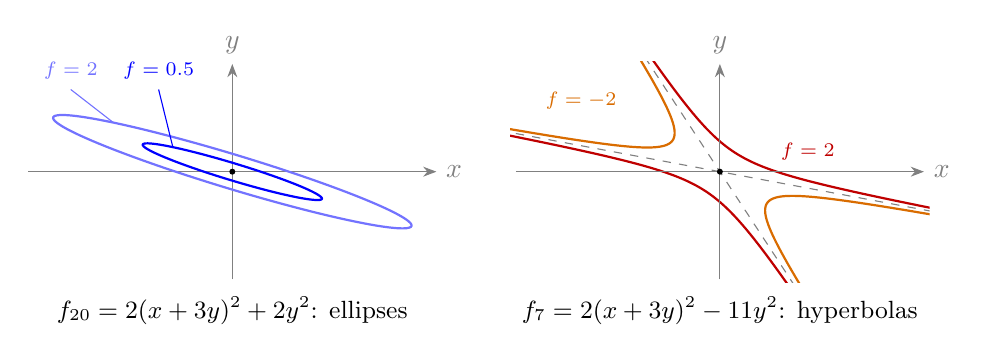
\begin{tikzpicture}[scale=0.72,>=Stealth]
  \begin{scope}
    \draw[->,gray] (-3.6,0) -- (3.6,0) node[right] {$x$};
    \draw[->,gray] (0,-1.9) -- (0,1.9) node[above] {$y$};
    \draw[thick,blue,domain=0:360,samples=90,smooth,variable=\t]
      plot ({0.5*(cos(\t)-3*sin(\t))},{0.5*sin(\t)});
    \draw[thick,blue!55,domain=0:360,samples=90,smooth,variable=\t]
      plot ({1.0*(cos(\t)-3*sin(\t))},{1.0*sin(\t)});
    \fill (0,0) circle (1.5pt);
    \draw[blue] (-1.049,0.433) -- (-1.3,1.45) node[above,font=\scriptsize] {$f=0.5$};
    \draw[blue!55] (-2.098,0.866) -- (-2.85,1.45) node[above,font=\scriptsize] {$f=2$};
    \node[font=\small] at (0,-2.45) {$f_{20}=2(x+3y)^2+2y^2$: ellipses};
  \end{scope}
  \begin{scope}[xshift=8.6cm]
    \begin{scope}
      \clip (-3.7,-1.95) rectangle (3.7,1.95);
      \draw[dashed,gray,domain=-3:3] plot ({-0.655*\x},{\x});
      \draw[dashed,gray,domain=-0.7:0.7] plot ({-5.345*\x},{\x});
      \foreach \s in {1,-1} {
        \draw[thick,red!75!black,domain=-2.6:2.6,samples=90,smooth,variable=\t]
          plot ({(\s)*cosh(\t)-3*0.4264*sinh(\t)},{0.4264*sinh(\t)});
        \draw[thick,orange!85!black,domain=-2.6:2.6,samples=90,smooth,variable=\t]
          plot ({sinh(\t)-3*(\s)*0.4264*cosh(\t)},{(\s)*0.4264*cosh(\t)});
      }
    \end{scope}
    \draw[->,gray] (-3.6,0) -- (3.6,0) node[right] {$x$};
    \draw[->,gray] (0,-1.9) -- (0,1.9) node[above] {$y$};
    \fill (0,0) circle (1.5pt);
    \node[red!75!black,font=\scriptsize,fill=white,inner sep=1pt] at (1.55,0.35) {$f=2$};
    \node[orange!85!black,font=\scriptsize,fill=white,inner sep=1pt] at (-2.45,1.25) {$f=-2$};
    \node[font=\small] at (0,-2.45) {$f_{7}=2(x+3y)^2-11y^2$: hyperbolas};
  \end{scope}
\end{tikzpicture}
\caption{Level curves of two quadratic forms that differ only in the corner entry. Left: for the
positive definite $A_{20}$ every level set $f=k>0$ is an ellipse around the minimum at the origin.
Right: for the indefinite $A_7$ the level sets $f=\pm2$ are hyperbolas; along the dashed lines
$x+3y=\pm\sqrt{11/2}\,y$ the form is zero, and between them it changes sign: a saddle point.}
\label{fig:u31-levels}
\end{figure}

\subsection{Second derivatives decide a minimum}

In one-variable calculus, $f'(x_0)=0$ makes $x_0$ a critical point and $f''(x_0)>0$ makes it a
minimum: the slope is increasing as we pass through. For $f(x_1,\dots,x_n)$ the first
derivatives must all vanish, and the role of $f''$ is played by the \emph{matrix of second
derivatives} (the Hessian)
\[
  H=\begin{bmatrix}\dfrac{\partial^2f}{\partial x_i\,\partial x_j}\end{bmatrix},
  \qquad\text{for two variables}\quad
  H=\begin{bmatrix}f_{xx}&f_{xy}\\f_{yx}&f_{yy}\end{bmatrix}.
\]
It is symmetric because mixed partial derivatives can be taken in either order: $f_{xy}=f_{yx}$.

\begin{proposition}[Second-derivative test]\label{prop:u31-hessian}
Let $f$ have continuous second derivatives near $\vb{x}_0$, with all first derivatives zero at
$\vb{x}_0$. If $H(\vb{x}_0)$ is positive definite, $\vb{x}_0$ is a strict local minimum. If
$H(\vb{x}_0)$ has a negative eigenvalue, $\vb{x}_0$ is not a minimum.
\end{proposition}
\begin{proof}[Sketch]
Taylor's formula gives $f(\vb{x}_0+\vb{h})=f(\vb{x}_0)+\tfrac12\vb{h}\T H(\vb{x}_0)\vb{h}+r(\vb{h})$ with
$r(\vb{h})/\|\vb{h}\|^2\to0$ as $\vb{h}\to\vb{0}$; the linear term is absent because the gradient is zero.
If $H$ is positive definite with smallest eigenvalue $\lambda_{\min}>0$, then
$\tfrac12\vb{h}\T H\vb{h}\ge\tfrac12\lambda_{\min}\|\vb{h}\|^2$ (expand $\vb{h}$ in the orthonormal
eigenvectors), which beats $r(\vb{h})$ for small $\vb{h}\ne\vb{0}$, so $f(\vb{x}_0+\vb{h})>f(\vb{x}_0)$. If
$H\vb{q}=\lambda\vb{q}$ with $\lambda<0$, moving along $\vb{h}=t\vb{q}$ gives
$f(\vb{x}_0+t\vb{q})-f(\vb{x}_0)=\tfrac12\lambda t^2\|\vb{q}\|^2+r(t\vb{q})<0$ for small $t\ne0$.
The full $\varepsilon$--$\delta$ details belong to multivariable calculus.
\end{proof}

For two variables the determinant test for $H$ is the familiar calculus rule: a minimum when
$f_{xx}>0$ and $f_{xx}f_{yy}>f_{xy}^2$. Linear algebra extends it to any number of variables,
where it is applied through pivots, determinants or eigenvalues of $H$. For a pure quadratic
$f(\vb{x})=\vb{x}\T A\vb{x}$ the Hessian is the constant matrix $2A$, so the local picture at the origin
is the global one: a bowl when $A$ is positive definite, a saddle when it is indefinite.

\begin{example}[Classifying critical points]\label{ex:u31-critical}
Let $f(x,y)=x^3+y^2-3xy$. Setting the first derivatives to zero,
\[
  f_x=3x^2-3y=0,\qquad f_y=2y-3x=0 .
\]
The second equation gives $y=\tfrac32x$; then $3x^2-\tfrac92x=0$, so $x=0$ or $x=\tfrac32$. The
critical points are $(0,0)$ and $(\tfrac32,\tfrac94)$. The Hessian is
$H=\left[\begin{smallmatrix}6x&-3\\-3&2\end{smallmatrix}\right]$.
\begin{itemize}
  \item At $(0,0)$: $H=\left[\begin{smallmatrix}0&-3\\-3&2\end{smallmatrix}\right]$ has
        $\det H=-9<0$, so one eigenvalue is negative: a saddle point, not a minimum.
  \item At $(\tfrac32,\tfrac94)$: $H=\left[\begin{smallmatrix}9&-3\\-3&2\end{smallmatrix}\right]$ has
        $D_1=9>0$ and $D_2=18-9=9>0$: positive definite, so a local minimum, with value
        $f=\tfrac{27}{8}+\tfrac{81}{16}-\tfrac{81}{8}=-\tfrac{27}{16}$.
\end{itemize}
\end{example}

\subsection{Ellipses, ellipsoids and principal axes}

Cut the bowl $z=\vb{x}\T A\vb{x}$ at height $1$. The cross-section $\vb{x}\T A\vb{x}=1$ is an ellipse in the plane,
an ellipsoid (a lopsided rugby ball) in $\R^3$. Cutting a saddle instead gives a hyperbola. The
spectral theorem says exactly how the ellipse sits.

\begin{theorem}[Principal axes]\label{thm:u31-axes}
Let $A=Q\Lambda Q\T$ be positive definite with orthonormal eigenvectors $\vb{q}_1,\dots,\vb{q}_n$. The
set $\vb{x}\T A\vb{x}=1$ is an ellipsoid whose axes point along the eigenvectors $\vb{q}_i$, with
half-lengths $1/\sqrt{\lambda_i}$.
\end{theorem}
\begin{proof}
In the coordinates $\vb{y}=Q\T\vb{x}$, which measure $\vb{x}$ along the perpendicular directions
$\vb{q}_i$ (a rotation, possibly with a reflection, which changes no shapes), the equation becomes
$\lambda_1y_1^2+\cdots+\lambda_ny_n^2=1$, the standard ellipsoid
$\sum y_i^2/(1/\sqrt{\lambda_i})^2=1$. Its axes are the $y_i$-axes, i.e.\ the $\vb{q}_i$ directions,
and the axis along $\vb{q}_i$ reaches $y_i=\pm1/\sqrt{\lambda_i}$.
\end{proof}

Large eigenvalues give short axes: the bowl rises steeply in that direction. Equal eigenvalues
give a round cross-section; two equal out of three give a rugby ball; the identity gives a
sphere.

\begin{example}[An ellipse tilted at \texorpdfstring{$45^\circ$}{45 degrees}]\label{ex:u31-ellipse}
For $A=\begin{bmatrix}5&4\\4&5\end{bmatrix}$ the equation $\vb{x}\T A\vb{x}=1$ reads $5x^2+8xy+5y^2=1$.
The eigenvalues are $9$ and $1$ (trace $10$, determinant $9$) with eigenvectors
$\vb{q}_1=(1,1)/\sqrt2$ and $\vb{q}_2=(1,-1)/\sqrt2$. So
\[
  5x^2+8xy+5y^2=9\Bigl(\frac{x+y}{\sqrt2}\Bigr)^2+1\Bigl(\frac{x-y}{\sqrt2}\Bigr)^2 ,
\]
and the ellipse has half-axis $1/\sqrt9=\tfrac13$ along $(1,1)$ and $1/\sqrt1=1$ along $(1,-1)$
(Figure~\ref{fig:u31-axes}). Check the endpoints: $(x,y)=\tfrac{1}{3\sqrt2}(1,1)$ gives
$\tfrac{5+8+5}{18}=1$, and $(x,y)=\tfrac{1}{\sqrt2}(1,-1)$ gives $\tfrac{5-8+5}{2}=1$.

For $K$ of Example~\ref{ex:u31-K}, $\vb{x}\T K\vb{x}=1$ is an ellipsoid with three different axes:
the longest, $1/\sqrt{2-\sqrt2}\approx1.31$, along $(1,\sqrt2,1)$; the middle one, $1/\sqrt2\approx0.71$,
along $(1,0,-1)$; the shortest, $1/\sqrt{2+\sqrt2}\approx0.54$, along $(1,-\sqrt2,1)$.
\end{example}

\begin{figure}[ht]\centering
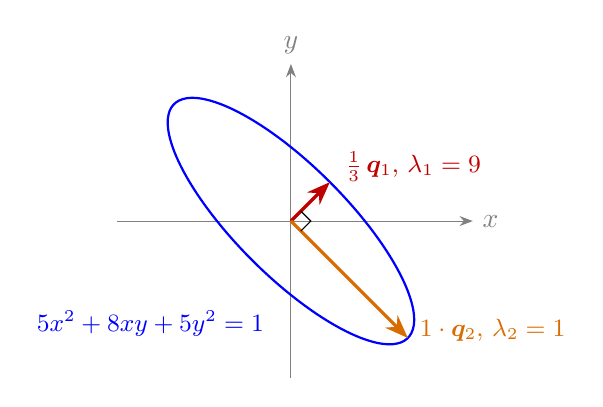
\begin{tikzpicture}[scale=2.1,>=Stealth]
  \draw[->,gray] (-1.05,0) -- (1.1,0) node[right] {$x$};
  \draw[->,gray] (0,-0.95) -- (0,0.95) node[above] {$y$};
  \draw[thick,blue,domain=0:360,samples=100,smooth,variable=\t]
    plot ({0.70711*(cos(\t)/3+sin(\t))},{0.70711*(cos(\t)/3-sin(\t))});
  \draw[->,very thick,red!75!black] (0,0) -- (0.2357,0.2357);
  \node[red!75!black,right,font=\small] at (0.27,0.33) {$\tfrac13\,\vb{q}_1$, $\lambda_1=9$};
  \draw[->,very thick,orange!85!black] (0,0) -- (0.70711,-0.70711);
  \node[orange!85!black,right,font=\small] at (0.72,-0.66) {$1\cdot\vb{q}_2$, $\lambda_2=1$};
  \draw (0.06,0.06) -- (0.12,0) -- (0.06,-0.06);
  \node[blue,font=\small] at (-0.85,-0.62) {$5x^2+8xy+5y^2=1$};
\end{tikzpicture}
\caption{The principal axes of $\vb{x}\T A\vb{x}=1$ for $A=\left[\begin{smallmatrix}5&4\\4&5\end{smallmatrix}\right]$
point along the eigenvectors; the half-lengths are $1/\sqrt{\lambda}$, so the large eigenvalue $9$
gives the short axis $\tfrac13$.}
\label{fig:u31-axes}
\end{figure}

\subsection{Exercises}

\begin{exercise}[Products of positive definite matrices]\label{exr:u31-AB}
When $A$ and $B$ are symmetric positive definite, $AB$ need not be symmetric, but its
eigenvalues are still positive. Prove this: start from $AB\vb{x}=\lambda\vb{x}$ and take the dot product
with $B\vb{x}$.
\end{exercise}
\begin{solution}
From $AB\vb{x}=\lambda\vb{x}$ with $\vb{x}\ne\vb{0}$, take the dot product with $B\vb{x}$:
\[
  (B\vb{x})\T AB\vb{x}=\lambda\,(B\vb{x})\T\vb{x}=\lambda\,\vb{x}\T B\vb{x},
\]
using $B\T=B$. The left side is $\vb{y}\T A\vb{y}$ with $\vb{y}=B\vb{x}\ne\vb{0}$ ($B$ is invertible), which is
positive because $A$ is positive definite. On the right, $\vb{x}\T B\vb{x}>0$ because $B$ is positive
definite. Hence $\lambda=\vb{y}\T A\vb{y}/\vb{x}\T B\vb{x}>0$. (Such a $\lambda$ is automatically real: the
quotient is real.) For instance $A=\left[\begin{smallmatrix}2&1\\1&1\end{smallmatrix}\right]$,
$B=\left[\begin{smallmatrix}1&1/2\\1/2&1\end{smallmatrix}\right]$ give the nonsymmetric
$AB=\left[\begin{smallmatrix}2.5&2\\1.5&1.5\end{smallmatrix}\right]$, whose eigenvalues
$2\pm\frac{\sqrt{13}}{2}\approx3.80,\,0.20$ are positive.
\end{solution}

\begin{exercise}[The form of a nonsymmetric matrix]\label{exr:u31-form}
Find the quadratic form $f(x,y)$ of $A=\left[\begin{smallmatrix}1&5\\7&9\end{smallmatrix}\right]$. Is it
always positive, always negative, or neither?
\end{exercise}
\begin{solution}
$f(x,y)=\begin{bmatrix}x&y\end{bmatrix}\begin{bmatrix}x+5y\\7x+9y\end{bmatrix}=x^2+5xy+7xy+9y^2=x^2+12xy+9y^2$.
Only the sum $5+7$ of the off-diagonal entries matters, so this is also the form of the
symmetric matrix $\left[\begin{smallmatrix}1&6\\6&9\end{smallmatrix}\right]$, whose determinant
$9-36=-27$ is negative. Hence $f$ takes both signs: $f(1,0)=1>0$ and $f(2,-2)=4-48+36=-8<0$.
Completing the square, $f=(x+6y)^2-27y^2$.
\end{solution}

\begin{exercise}[A parameter in the corner]\label{exr:u31-param}
For which $c$ is $B=\left[\begin{smallmatrix}2&-1&-1\\-1&2&-1\\-1&-1&2+c\end{smallmatrix}\right]$ positive
definite? Positive semidefinite? Confirm with pivots and by completing squares, and find
$\vb{x}\ne\vb{0}$ with $\vb{x}\T B\vb{x}=0$ when $c=0$.
\end{exercise}
\begin{solution}
\emph{Determinants.} $D_1=2$, $D_2=4-1=3$, and expanding along row~1,
$D_3=2\bigl(2(2+c)-1\bigr)+1\bigl(-(2+c)-1\bigr)-1\bigl(1+2\bigr)=(6+4c)-(3+c)-3=3c$. So $B$ is
positive definite for $c>0$ and positive semidefinite for $c\ge0$ (for $c<0$, $\det B<0$ forces a
negative eigenvalue).

\emph{Pivots.} Add $\tfrac12$ row~1 to rows 2 and 3: rows become $(0,\tfrac32,-\tfrac32)$ and
$(0,-\tfrac32,\tfrac32+c)$; add the new row~2 to row~3: $(0,0,c)$. Pivots $2,\ \tfrac32,\ c$, which are
the ratios $2,\ 3/2,\ 3c/3$ of the determinants.

\emph{Squares.} $\vb{x}\T B\vb{x}=2x^2+2y^2+(2+c)z^2-2xy-2xz-2yz
=2\bigl(x-\tfrac12y-\tfrac12z\bigr)^2+\tfrac32(y-z)^2+cz^2$. For $c=0$ this vanishes when $y=z$ and
$x=\tfrac12(y+z)$, for example at $\vb{x}=(1,1,1)$; indeed every row of $B$ then sums to zero, so
$(1,1,1)$ is in the nullspace.
\end{solution}

\begin{exercise}[How big can the cross term be?]\label{exr:u31-b}
For which $b$ is $\left[\begin{smallmatrix}1&b\\b&9\end{smallmatrix}\right]$ positive definite? For
$b=4$, find a vector that makes the form negative.
\end{exercise}
\begin{solution}
Need $1>0$ and $9-b^2>0$, so $-3<b<3$. At $b=\pm3$ the matrix is only semidefinite:
$x^2\pm6xy+9y^2=(x\pm3y)^2$. For $b=4$, $x^2+8xy+9y^2=(x+4y)^2-7y^2$; choosing $x+4y=0$, $y=1$,
i.e.\ $(x,y)=(-4,1)$, gives $16-32+9=-7<0$.
\end{solution}

% unit: u32
% sources: sources/091-similar-matrices-and-jordan-form.txt, sources/055-lecture-28-similar-matrices-and-jordan-form.txt, sources/215-mit18-06scf11-ses3-4sum-pdf-download-file.txt, sources/056-problem-solving-similar-matrices.txt, sources/216-mit18-06scf11-ses3-4prob-pdf-download-file.txt, sources/217-mit18-06scf11-ses3-4sol-pdf-download-file.txt
\section{Similar matrices and Jordan form}\label{sec:u32}

This unit finishes the story of positive definite matrices by showing where they come from,
$A\T A$, and then turns to a new way of organizing all square matrices. Two matrices are
\emph{similar} when one is $M^{-1}AM$ for some invertible $M$. Similar matrices share their
eigenvalues, so the square matrices fall into families, and in each family we look for the
simplest member. When $A$ has $n$ independent eigenvectors that member is the diagonal $\Lambda$;
when eigenvectors are missing it is the Jordan form. Diagonalization (Section~\ref{sec:u24}) was
the first example of similarity; Section~\ref{sec:u35} will show that similar matrices are the
same linear transformation seen in different bases.

\subsection{Where positive definite matrices come from}

Positive definiteness behaves like positivity of numbers. Two quick facts show which of the
four tests of Section~\ref{sec:u31} to reach for.

\begin{proposition}[Inverses and sums]\label{prop:u32-inverse-sum}
If $A$ and $B$ are symmetric positive definite, so are $A^{-1}$ and $A+B$.
\end{proposition}
\begin{proof}
$A^{-1}$ is symmetric because $(A^{-1})\T=(A\T)^{-1}=A^{-1}$, and its eigenvalues $1/\lambda_i$ are
positive: the eigenvalue test is the natural one here, since we know nothing about the pivots
of $A^{-1}$. For $A+B$ we know neither eigenvalues nor pivots, but the energy test is immediate:
for $\vb{x}\ne\vb{0}$, $\vb{x}\T(A+B)\vb{x}=\vb{x}\T A\vb{x}+\vb{x}\T B\vb{x}>0$.
\end{proof}

The most important source is a rectangular matrix. In least squares (Section~\ref{sec:u18}) an
$m\times n$ matrix $A$ led to the square symmetric matrix $A\T A$. Like the square of a number, it
cannot be negative.

\begin{theorem}[\texorpdfstring{$A\T A$}{ATA} is positive definite]\label{thm:u32-ata}
For any $m\times n$ matrix $A$, the matrix $A\T A$ is symmetric positive semidefinite. It is
positive definite exactly when $A$ has independent columns (rank $n$).
\end{theorem}
\begin{proof}
Symmetry: $(A\T A)\T=A\T(A\T)\T=A\T A$. For the energy, move the parentheses:
\[
  \vb{x}\T(A\T A)\vb{x}=(A\vb{x})\T(A\vb{x})=\|A\vb{x}\|^2\ge0 .
\]
This is zero only when $A\vb{x}=\vb{0}$. If the columns are independent, $\Nul{A}=\{\vb{0}\}$ and so
$\vb{x}\T A\T A\vb{x}>0$ for all $\vb{x}\ne\vb{0}$. If the columns are dependent, a nonzero $\vb{x}$ in the
nullspace gives $\vb{x}\T A\T A\vb{x}=0$, so $A\T A$ is only semidefinite.
\end{proof}

\begin{example}[Two rectangular matrices]\label{ex:u32-ata}
For the line-fitting matrix $A=\left[\begin{smallmatrix}1&0\\1&1\\1&2\end{smallmatrix}\right]$, the columns
are independent and $A\T A=\left[\begin{smallmatrix}3&3\\3&5\end{smallmatrix}\right]$ has upper-left
determinants $3$ and $15-9=6$: positive definite, so the normal equations $A\T A\hat{\vb{x}}=A\T\vb{b}$
always have a unique solution. For $B=\left[\begin{smallmatrix}1&2\\2&4\\3&6\end{smallmatrix}\right]$ the
second column is twice the first, and $B\T B=\left[\begin{smallmatrix}14&28\\28&56\end{smallmatrix}\right]$
has determinant $784-784=0$: semidefinite only, with $\vb{x}=(2,-1)$ giving
$\vb{x}\T B\T B\vb{x}=\|B\vb{x}\|^2=0$.
\end{example}

A practical bonus: elimination on a positive definite matrix never needs row exchanges, since
all pivots are positive; there are no zeros, or dangerously small numbers, in the pivot
positions. These are the best matrices to compute with.

\subsection{Similar matrices share eigenvalues}

\begin{definition}[Similar matrices]\label{def:u32-similar}
Two $n\times n$ matrices $A$ and $B$ are \emph{similar} if $B=M^{-1}AM$ for some invertible
matrix $M$.
\end{definition}

If $A$ has $n$ independent eigenvectors in the columns of $X$, then $X^{-1}AX=\Lambda$
(Section~\ref{sec:u24}): $A$ is similar to $\Lambda$, with $M=X$. Any other invertible $M$ also gives
a similar matrix, just not a diagonal one.

\begin{example}[A family with eigenvalues 3 and 1]\label{ex:u32-family31}
Let $A=\begin{bmatrix}2&1\\1&2\end{bmatrix}$, with eigenvalues $3$ and $1$, so $A$ is similar to
$\Lambda=\left[\begin{smallmatrix}3&0\\0&1\end{smallmatrix}\right]$. Now choose any invertible $M$, say
$M=\left[\begin{smallmatrix}1&4\\0&1\end{smallmatrix}\right]$, whose inverse is
$M^{-1}=\left[\begin{smallmatrix}1&-4\\0&1\end{smallmatrix}\right]$. Then
\[
  AM=\begin{bmatrix}2&9\\1&6\end{bmatrix},\qquad
  B=M^{-1}AM=\begin{bmatrix}1&-4\\0&1\end{bmatrix}\begin{bmatrix}2&9\\1&6\end{bmatrix}
   =\begin{bmatrix}-2&-15\\1&6\end{bmatrix}.
\]
Nothing about $B$ looks special, but $\tr B=-2+6=4=3+1$ and $\det B=-12+15=3=3\cdot1$: its
eigenvalues are again $3$ and $1$. Other members of the same family are the triangular matrices
$\left[\begin{smallmatrix}3&7\\0&1\end{smallmatrix}\right]$ and
$\left[\begin{smallmatrix}1&7\\0&3\end{smallmatrix}\right]$.
\end{example}

\begin{theorem}[What similar matrices share]\label{thm:u32-same}
If $B=M^{-1}AM$, then $A$ and $B$ have the same characteristic polynomial, hence the same
eigenvalues, trace and determinant. If $A\vb{x}=\lambda\vb{x}$ then $B(M^{-1}\vb{x})=\lambda(M^{-1}\vb{x})$, and
for each $\lambda$ the two matrices have the same number of independent eigenvectors.
\end{theorem}
\begin{proof}
Since $M^{-1}(\lambda I)M=\lambda I$,
\[
  \det(B-\lambda I)=\det\bigl(M^{-1}(A-\lambda I)M\bigr)=\det M^{-1}\,\det(A-\lambda I)\,\det M=\det(A-\lambda I).
\]
For the eigenvectors, insert $MM^{-1}=I$: from $A\vb{x}=\lambda\vb{x}$ we get $AMM^{-1}\vb{x}=\lambda\vb{x}$, and
multiplying on the left by $M^{-1}$ gives $(M^{-1}AM)(M^{-1}\vb{x})=\lambda(M^{-1}\vb{x})$. So $M^{-1}$
carries the eigenvectors of $A$ for $\lambda$ onto eigenvectors of $B$ for $\lambda$; it is
invertible, so it maps independent vectors to independent vectors, and $M$ carries them back.
\end{proof}

The eigenvalues stay; the eigenvectors move (by $M^{-1}$). Similarity is also an equivalence
relation: $A=I^{-1}AI$; if $B=M^{-1}AM$ then $A=MBM^{-1}=(M^{-1})^{-1}B(M^{-1})$; and if also
$C=N^{-1}BN$ then $C=(MN)^{-1}A(MN)$. So the $n\times n$ matrices split into disjoint families of
mutually similar matrices.

\begin{corollary}[Distinct eigenvalues]\label{cor:u32-distinct}
If $A$ and $B$ have the same $n$ distinct eigenvalues, they are similar.
\end{corollary}
\begin{proof}
Distinct eigenvalues give independent eigenvectors, so $A=X\Lambda X^{-1}$ and $B=Y\Lambda Y^{-1}$
with the same $\Lambda$. Then $B=Y X^{-1}AXY^{-1}=M^{-1}AM$ with $M=XY^{-1}$.
\end{proof}

So when the eigenvalues are distinct, the family is simply ``all matrices with these
eigenvalues'', and its best member is $\Lambda$.

\subsection{Repeated eigenvalues: two families}

Now let $\lambda_1=\lambda_2=4$. The trouble with a repeated eigenvalue is that there may not be a
full set of eigenvectors. The $2\times2$ matrices with eigenvalues $4,4$ split into \emph{two}
families.

\emph{The loner.} $4I$ is similar only to itself, because $M^{-1}(4I)M=4M^{-1}M=4I$ for every $M$.

\emph{Everyone else.} Every other matrix with eigenvalues $4,4$ is similar to the
\emph{Jordan block}
\[
  J=\begin{bmatrix}4&1\\0&4\end{bmatrix}.
\]
$J$ is not diagonalizable: $J-4I=\left[\begin{smallmatrix}0&1\\0&0\end{smallmatrix}\right]$ has rank $1$,
so there is only one independent eigenvector, $(1,0)$. If $J$ were diagonalizable it would be
similar to $4I$, which is similar only to itself. To find more members of $J$'s family, choose
any trace $8$ and determinant $16$:
\[
  \begin{bmatrix}5&1\\-1&3\end{bmatrix},\qquad
  \begin{bmatrix}4&0\\17&4\end{bmatrix},\qquad
  \begin{bmatrix}a&b\\(8a-a^2-16)/b&8-a\end{bmatrix}\ (b\ne0).
\]
For the last one, the trace is $a+8-a=8$ and the determinant is
$a(8-a)-(8a-a^2-16)=16$. None of these is $4I$, so none is diagonalizable, and each has a single
line of eigenvectors. Figure~\ref{fig:u32-families} pictures the families.

\begin{figure}[ht]\centering
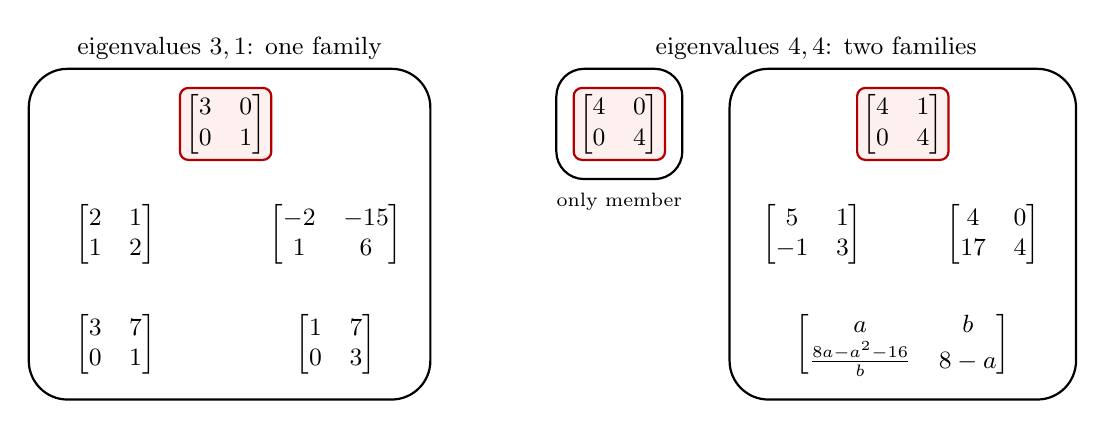
\begin{tikzpicture}[font=\small,
  best/.style={draw=red!70!black,thick,fill=red!6,rounded corners=3pt,inner sep=2pt}]
  \draw[thick,rounded corners=14pt] (-2.5,-2.6) rectangle (2.6,1.6);
  \node[above] at (0.05,1.6) {eigenvalues $3,1$: one family};
  \node[best] at (0,0.9) {$\begin{bmatrix}3&0\\0&1\end{bmatrix}$};
  \node at (-1.4,-0.5) {$\begin{bmatrix}2&1\\1&2\end{bmatrix}$};
  \node at (1.4,-0.5) {$\begin{bmatrix}-2&-15\\1&6\end{bmatrix}$};
  \node at (-1.4,-1.9) {$\begin{bmatrix}3&7\\0&1\end{bmatrix}$};
  \node at (1.4,-1.9) {$\begin{bmatrix}1&7\\0&3\end{bmatrix}$};
  \draw[thick,rounded corners=10pt] (4.2,0.2) rectangle (5.8,1.6);
  \node[best] at (5.0,0.9) {$\begin{bmatrix}4&0\\0&4\end{bmatrix}$};
  \node[below,align=center,font=\scriptsize] at (5.0,0.15) {only member};
  \draw[thick,rounded corners=14pt] (6.4,-2.6) rectangle (10.8,1.6);
  \node[best] at (8.6,0.9) {$\begin{bmatrix}4&1\\0&4\end{bmatrix}$};
  \node at (7.45,-0.5) {$\begin{bmatrix}5&1\\-1&3\end{bmatrix}$};
  \node at (9.75,-0.5) {$\begin{bmatrix}4&0\\17&4\end{bmatrix}$};
  \node at (8.6,-1.9) {$\begin{bmatrix}a&b\\\frac{8a-a^2-16}{b}&8-a\end{bmatrix}$};
  \node[above] at (7.5,1.6) {eigenvalues $4,4$: two families};
\end{tikzpicture}
\caption{Families of similar $2\times2$ matrices. Within a family every pair is connected by some
$M^{-1}AM$; the framed member is the simplest one (its Jordan form). With distinct eigenvalues
$3,1$ there is one family and its best member is $\Lambda$. With eigenvalues $4,4$ the loner $4I$
forms a family by itself, and all the other matrices are similar to the Jordan block.}
\label{fig:u32-families}
\end{figure}

\begin{example}[Bringing a matrix to its Jordan block]\label{ex:u32-chain}
Show directly that $B=\begin{bmatrix}5&1\\-1&3\end{bmatrix}$ is similar to $J=\begin{bmatrix}4&1\\0&4\end{bmatrix}$.
The lectures do not compute Jordan forms in general, but for a $2\times2$ block the idea is short.
We want $M=[\vb{x}_1\ \vb{x}_2]$ with $BM=MJ$, i.e.
\[
  B\vb{x}_1=4\vb{x}_1,\qquad B\vb{x}_2=\vb{x}_1+4\vb{x}_2\quad\text{(equivalently } (B-4I)\vb{x}_2=\vb{x}_1\text{)}.
\]
Here $B-4I=\left[\begin{smallmatrix}1&1\\-1&-1\end{smallmatrix}\right]$ has rank $1$; its nullspace gives
the eigenvector $\vb{x}_1=(1,-1)$, and $(B-4I)\vb{x}_2=\vb{x}_1$ is solved by $\vb{x}_2=(1,0)$. With
$M=\left[\begin{smallmatrix}1&1\\-1&0\end{smallmatrix}\right]$:
\[
  BM=\begin{bmatrix}5&1\\-1&3\end{bmatrix}\begin{bmatrix}1&1\\-1&0\end{bmatrix}=\begin{bmatrix}4&5\\-4&-1\end{bmatrix},
  \qquad
  MJ=\begin{bmatrix}1&1\\-1&0\end{bmatrix}\begin{bmatrix}4&1\\0&4\end{bmatrix}=\begin{bmatrix}4&5\\-4&-1\end{bmatrix}.
\]
They agree, $M$ is invertible ($\det M=1$), and so $M^{-1}BM=J$.
\end{example}

\subsection{Jordan blocks and Jordan's theorem}

\begin{definition}[Jordan block, Jordan matrix]\label{def:u32-jordan}
A \emph{Jordan block} $J_i$ of size $k$ has one eigenvalue $\lambda_i$ repeated on the diagonal,
ones just above the diagonal, and zeros elsewhere:
\[
  J_i=\begin{bmatrix}\lambda_i&1&&\\&\lambda_i&\ddots&\\&&\ddots&1\\&&&\lambda_i\end{bmatrix}.
\]
Its only independent eigenvector is $\vb{e}_1$. A \emph{Jordan matrix} is a block diagonal matrix
whose diagonal blocks are Jordan blocks:
\[
  J=\begin{bmatrix}J_1&&\\&\ddots&\\&&J_d\end{bmatrix}.
\]
\end{definition}

\begin{theorem}[Jordan form]\label{thm:u32-jordan}
Every square matrix $A$ is similar to a Jordan matrix $J=M^{-1}AM$. The eigenvalues of $A$ sit on
the diagonal of $J$; the number of blocks $d$ equals the number of independent eigenvectors of
$A$, one eigenvector per block; and $J$ is unique apart from the order of the blocks.
\end{theorem}

The proof is long, and the course states the theorem without it; a proof is in the appendix on
the Jordan form in Strang's \emph{Introduction to Linear Algebra}, and in any advanced linear
algebra text. Two cases summarize it.
If $A$ has $n$ distinct eigenvalues, every block has size $1$ and $J=\Lambda$: there are $d=n$
blocks and eigenvectors. If eigenvectors are missing, $J$ has $n-d$ ones above the diagonal,
one for each missing eigenvector. The uniqueness part, which is what separates families, can be
proved with one invariant.

\begin{proposition}[Ranks of powers are similarity invariants]\label{prop:u32-ranks}
If $B=M^{-1}AM$ then $\rank\,(B-\lambda I)^k=\rank\,(A-\lambda I)^k$ for every number $\lambda$ and every
$k\ge1$.
\end{proposition}
\begin{proof}
$B-\lambda I=M^{-1}(A-\lambda I)M$, and the inner factors $MM^{-1}$ cancel in a power:
$(B-\lambda I)^k=M^{-1}(A-\lambda I)^kM$. Multiplying by invertible matrices on either side does not
change the rank.
\end{proof}

Counting eigenvectors uses only $k=1$ (the nullity of $A-\lambda I$). Higher powers see the
sizes of the blocks, as the next example shows.

\begin{example}[Same eigenvalues, same eigenvector count, not similar]\label{ex:u32-4by4}
Compare the $4\times4$ matrices
\[
  A=\begin{bmatrix}0&1&0&0\\0&0&1&0\\0&0&0&0\\0&0&0&0\end{bmatrix},\qquad
  C=\begin{bmatrix}0&1&0&0\\0&0&0&0\\0&0&0&1\\0&0&0&0\end{bmatrix}.
\]
Both are triangular with four zero eigenvalues. Both have rank $2$, so each nullspace (the
eigenvectors for $\lambda=0$) has dimension $4-2=2$: two eigenvectors and two missing. But $A$
consists of a $3\times3$ block and a $1\times1$ block, while $C$ consists of two $2\times2$ blocks.
The squares tell them apart: $A^2$ has a single $1$ in position $(1,3)$, so $\rank A^2=1$,
whereas $C^2=0$. By Proposition~\ref{prop:u32-ranks}, $A$ and $C$ are not similar.

Changing the $(1,3)$ entry of $A$ from $0$ to $7$ gives a matrix $A'$ with the same ranks of
powers ($\rank A'=2$, $\rank A'^2=1$, $A'^3=0$); it is similar to $A$, and $A$ is the Jordan form of
that family: a $1$ above the diagonal for every missing eigenvector, zeros elsewhere.
\end{example}

\begin{trap}
Equal eigenvalues do not make matrices similar, and neither do equal eigenvalues plus equal
numbers of eigenvectors. $\left[\begin{smallmatrix}4&0\\0&4\end{smallmatrix}\right]$ and
$\left[\begin{smallmatrix}4&1\\0&4\end{smallmatrix}\right]$ share trace and determinant, and $A$, $C$ above
share even the eigenvector count. Only for distinct eigenvalues is ``same eigenvalues'' enough.
Note also that the Jordan form, though perfect for algebra, is useless numerically: the
slightest change in the entries splits repeated eigenvalues and changes the blocks.
\end{trap}

\subsection{Exercises}

\begin{exercise}[Jordan matrices with different block sizes]\label{exr:u32-JK}
Let $J$ have Jordan blocks of sizes $2,2$ and $K$ blocks of sizes $3,1$, all with eigenvalue $0$:
\[
  J=\begin{bmatrix}0&1&0&0\\0&0&0&0\\0&0&0&1\\0&0&0&0\end{bmatrix},\qquad
  K=\begin{bmatrix}0&1&0&0\\0&0&1&0\\0&0&0&0\\0&0&0&0\end{bmatrix}.
\]
Both have two independent eigenvectors. Show that if $JM=MK$ then $M$ is not invertible, so $J$
and $K$ are not similar.
\end{exercise}
\begin{solution}
Write $M=(m_{ij})$. Multiplying by $J$ on the left shifts rows: row~1 of $JM$ is row~2 of $M$,
row~3 of $JM$ is row~4 of $M$, rows 2 and 4 are zero. Multiplying by $K$ on the right shifts
columns: column~2 of $MK$ is column~1 of $M$, column~3 is column~2, columns 1 and 4 are zero:
\[
  JM=\begin{bmatrix}m_{21}&m_{22}&m_{23}&m_{24}\\0&0&0&0\\m_{41}&m_{42}&m_{43}&m_{44}\\0&0&0&0\end{bmatrix},
  \qquad
  MK=\begin{bmatrix}0&m_{11}&m_{12}&0\\0&m_{21}&m_{22}&0\\0&m_{31}&m_{32}&0\\0&m_{41}&m_{42}&0\end{bmatrix}.
\]
Comparing entries: column~1 gives $m_{21}=m_{41}=0$; row~2 gives $m_{21}=m_{22}=0$ and row~4 gives
$m_{41}=m_{42}=0$; then entry $(1,2)$ gives $m_{11}=m_{22}=0$ and entry $(3,2)$ gives
$m_{31}=m_{42}=0$. So the whole first column $(m_{11},m_{21},m_{31},m_{41})$ is zero and $M$ is
singular. A similarity $K=M^{-1}JM$ would require an invertible $M$ with $JM=MK$; none exists.
(Ranks of squares give the same verdict: $J^2=0$ but $\rank K^2=1$.)
\end{solution}

\begin{exercise}[True statements about similarity]\label{exr:u32-true}
Explain why each statement is true.
\begin{enumerate}[(a)]
  \item If $A$ is similar to $B$ then $A^2$ is similar to $B^2$.
  \item $A^2$ and $B^2$ can be similar when $A$ and $B$ are not.
  \item $\left[\begin{smallmatrix}3&0\\0&4\end{smallmatrix}\right]$ is similar to
        $\left[\begin{smallmatrix}3&1\\0&4\end{smallmatrix}\right]$.
  \item $\left[\begin{smallmatrix}3&0\\0&3\end{smallmatrix}\right]$ is not similar to
        $\left[\begin{smallmatrix}3&1\\0&3\end{smallmatrix}\right]$.
  \item If $B$ is obtained from $A$ by exchanging rows 1 and 2 and then columns 1 and 2, then $B$
        is similar to $A$.
\end{enumerate}
\end{exercise}
\begin{solution}
\begin{enumerate}[(a)]
  \item If $A=M^{-1}BM$ then $A^2=M^{-1}BMM^{-1}BM=M^{-1}B^2M$.
  \item Take $A=\left[\begin{smallmatrix}0&0\\0&0\end{smallmatrix}\right]$ and
        $B=\left[\begin{smallmatrix}0&1\\0&0\end{smallmatrix}\right]$. Then $A^2=B^2=0$, which are
        certainly similar, but only the zero matrix is similar to the zero matrix, so $A$ and $B$
        are not similar.
  \item The eigenvalues $3$ and $4$ are distinct, so both matrices are similar to
        $\operatorname{diag}(3,4)$ (Corollary~\ref{cor:u32-distinct}). Explicitly, with
        $M=\left[\begin{smallmatrix}1&1\\0&1\end{smallmatrix}\right]$,
        $M^{-1}\left[\begin{smallmatrix}3&1\\0&4\end{smallmatrix}\right]M
        =\left[\begin{smallmatrix}1&-1\\0&1\end{smallmatrix}\right]\left[\begin{smallmatrix}3&4\\0&4\end{smallmatrix}\right]
        =\left[\begin{smallmatrix}3&0\\0&4\end{smallmatrix}\right]$.
  \item For $3I$ every vector is an eigenvector; for the second matrix only the line through
        $(1,0)$. Similar matrices have the same number of independent eigenvectors.
  \item Exchanging rows 1 and 2 is left multiplication by the permutation matrix $P$ obtained from
        $I$ by exchanging its rows 1 and 2; exchanging columns 1 and 2 is right multiplication by
        the same $P$. So $B=PAP$, and since $P^{-1}=P$, $B=P^{-1}AP$.
\end{enumerate}
\end{solution}

\begin{exercise}[Polynomials, distinct eigenvalues and Jordan blocks]\label{exr:u32-recitation}
\begin{enumerate}[(a)]
  \item If $A$ and $B$ are similar, show that $2A^3+A-3I$ is similar to $2B^3+B-3I$.
  \item If $A$ and $B$ are $3\times3$ matrices with eigenvalues $1,0,-1$, must they be similar?
  \item Are $J_1=\left[\begin{smallmatrix}-1&1&0\\0&-1&1\\0&0&-1\end{smallmatrix}\right]$ and
        $J_2=\left[\begin{smallmatrix}-1&1&0\\0&-1&0\\0&0&-1\end{smallmatrix}\right]$ similar?
\end{enumerate}
\end{exercise}
\begin{solution}
\begin{enumerate}[(a)]
  \item Let $B=MAM^{-1}$. Then $MA^3M^{-1}=(MAM^{-1})^3=B^3$ and $MIM^{-1}=I$, so
        $M(2A^3+A-3I)M^{-1}=2B^3+B-3I$. The same works for any polynomial in $A$.
  \item Yes. Three distinct eigenvalues make both diagonalizable with the same
        $\Lambda=\operatorname{diag}(1,0,-1)$: $A=S\Lambda S^{-1}$ and $B=T\Lambda T^{-1}$, so
        $B=(TS^{-1})A(TS^{-1})^{-1}$. Similar to the same matrix means similar to each other.
  \item No. Both have the single eigenvalue $-1$, but $J_1+I$ has rank $2$ (a nullspace of
        dimension $1$: one eigenvector), while $J_2+I$ has rank $1$ (a nullspace of dimension $2$:
        two eigenvectors). Similar matrices have the same number of independent eigenvectors.
\end{enumerate}
\end{solution}

\begin{exercise}[When is \texorpdfstring{$A\T A$}{ATA} invertible?]\label{exr:u32-ata}
Let $A=\left[\begin{smallmatrix}1&1\\1&t\\1&t^2\end{smallmatrix}\right]$. For which $t$ is $A\T A$ positive
definite? Compute $A\T A$ for $t=1$ and exhibit $\vb{x}\ne\vb{0}$ with $\vb{x}\T A\T A\vb{x}=0$.
\end{exercise}
\begin{solution}
By Theorem~\ref{thm:u32-ata}, $A\T A$ is positive definite exactly when the columns $(1,1,1)$ and
$(1,t,t^2)$ are independent, i.e.\ unless $(1,t,t^2)$ is a multiple of $(1,1,1)$, which happens only
for $t=1$. So: positive definite for every $t\ne1$. At $t=1$ both columns are $(1,1,1)$ and
$A\T A=\left[\begin{smallmatrix}3&3\\3&3\end{smallmatrix}\right]$; the vector $\vb{x}=(1,-1)$ gives
$A\vb{x}=\vb{0}$, so $\vb{x}\T A\T A\vb{x}=3-3-3+3=0$.
\end{solution}

% unit: u33
% sources: sources/084-singular-value-decomposition.txt, sources/057-lecture-29-singular-value-decomposition.txt, sources/218-mit18-06scf11-ses3-5sum-pdf-download-file.txt, sources/058-problem-solving-determinants-and-volumecomputing-the-singula.txt, sources/219-mit18-06scf11-ses3-5prob-pdf-download-file.txt, sources/220-mit18-06scf11-ses3-5sol-pdf-download-file.txt; short s05 (svd-circle-to-ellipse)
\section{Singular value decomposition}\label{sec:u33}

The singular value decomposition, the SVD, is the final and best factorization of a matrix:
\[
  A=U\Sigma V\T ,\qquad U \text{ orthogonal},\quad \Sigma \text{ diagonal},\quad V \text{ orthogonal}.
\]
Unlike every earlier factorization, it works for \emph{any} matrix: rectangular, singular, not
symmetric. We have met two relatives. A symmetric positive definite matrix is $Q\Lambda Q\T$
(Section~\ref{sec:u29}), which is already of this form with $U=V=Q$. A diagonalizable matrix is
$X\Lambda X^{-1}$ (Section~\ref{sec:u24}), but $X$ is usually not orthogonal and many matrices have
no such factorization at all. The SVD keeps the diagonal middle and the orthogonal outsides by
paying one price: two different orthogonal matrices, $U$ on the left and $V$ on the right. The
construction uses everything from the last units: $A\T A$ is symmetric positive semidefinite
(Section~\ref{sec:u32}), so the spectral theorem applies to it, and the result produces
orthonormal bases for all four fundamental subspaces (Section~\ref{sec:u11}).

\subsection{Every matrix turns a circle into an ellipse}

Feed a $2\times2$ matrix every unit vector, the whole unit circle. The outputs always form an
ellipse. The SVD explains why: some pair of perpendicular unit vectors goes to perpendicular
vectors, and those are the axes of the ellipse.

\begin{example}[Perpendicular in, perpendicular out]\label{ex:u33-short}
Let $A=\begin{bmatrix}6&8\\-4&3\end{bmatrix}$ act on the unit circle.

\emph{The ordinary axes get skewed.} $A(1,0)=(6,-4)$ and $A(0,1)=(8,3)$. Their dot product is
$48-12=36\ne0$: the right angle between $\vb{e}_1$ and $\vb{e}_2$ is lost.

\emph{A better pair.} Take the perpendicular unit vectors $\vb{v}_1=(0.6,\,0.8)$ and
$\vb{v}_2=(-0.8,\,0.6)$. Then
\begin{align*}
  A\vb{v}_1&=(3.6+6.4,\ -2.4+2.4)=(10,\,0)=10\,(1,0),\\
  A\vb{v}_2&=(-4.8+4.8,\ 3.2+1.8)=(0,\,5)=5\,(0,1).
\end{align*}
The outputs are perpendicular too. So $\sigma_1=10$, $\sigma_2=5$, $\vb{u}_1=(1,0)$, $\vb{u}_2=(0,1)$, and
\[
  A=U\Sigma V\T=\begin{bmatrix}1&0\\0&1\end{bmatrix}\begin{bmatrix}10&0\\0&5\end{bmatrix}
  \begin{bmatrix}0.6&0.8\\-0.8&0.6\end{bmatrix}.
\]
The unit circle becomes the ellipse with semi-axes $10$ along $\vb{u}_1$ and $5$ along $\vb{u}_2$
(Figure~\ref{fig:u33-circle}).

\emph{Checks.} $A\T A=\left[\begin{smallmatrix}6&-4\\8&3\end{smallmatrix}\right]\left[\begin{smallmatrix}6&8\\-4&3\end{smallmatrix}\right]
=\left[\begin{smallmatrix}52&36\\36&73\end{smallmatrix}\right]$ has trace $125=100+25$ and determinant
$52\cdot73-36^2=3796-1296=2500=100\cdot25$, so its eigenvalues are $100=10^2$ and $25=5^2$. And the
area factor is $|\det A|=|18+32|=50=\sigma_1\sigma_2$: the ellipse has area $\pi\cdot10\cdot5=50\pi$,
fifty times the circle's.
\end{example}

\begin{figure}[ht]\centering
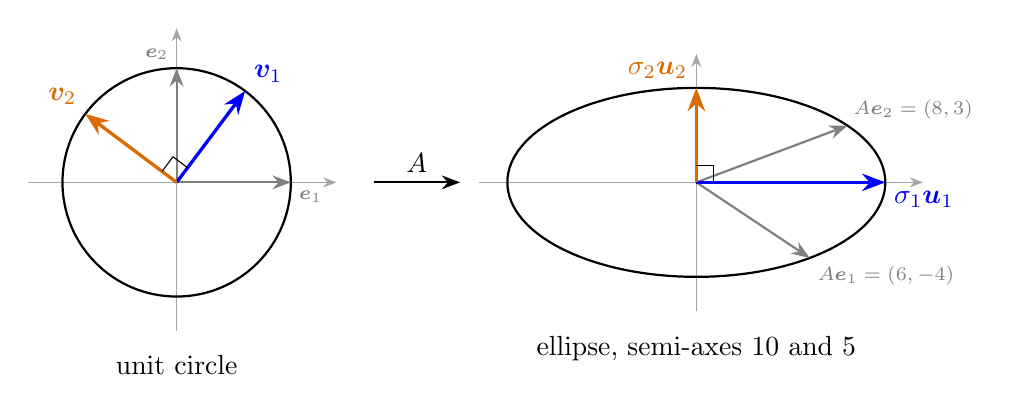
\begin{tikzpicture}[>=Stealth]
  \begin{scope}[scale=1.45]
    \draw[->,gray!70] (-1.3,0) -- (1.4,0);
    \draw[->,gray!70] (0,-1.3) -- (0,1.35);
    \draw[thick] (0,0) circle (1);
    \draw[->,gray,thick] (0,0) -- (1,0) node[below right=-1pt,font=\scriptsize] {$\vb{e}_1$};
    \draw[->,gray,thick] (0,0) -- (0,1) node[above left=-1pt,font=\scriptsize] {$\vb{e}_2$};
    \draw[->,very thick,blue] (0,0) -- (0.6,0.8) node[above right=-1pt] {$\vb{v}_1$};
    \draw[->,very thick,orange!85!black] (0,0) -- (-0.8,0.6) node[above left=-1pt] {$\vb{v}_2$};
    \draw (0.096,0.128) -- (-0.032,0.224) -- (-0.128,0.096);
    \node at (0,-1.6) {unit circle};
  \end{scope}
  \draw[->,thick] (2.5,0) -- node[above] {$A$} (3.6,0);
  \begin{scope}[xshift=6.6cm,scale=0.24]
    \draw[->,gray!70] (-11.5,0) -- (12,0);
    \draw[->,gray!70] (0,-6.8) -- (0,6.8);
    \draw[thick] (0,0) ellipse (10 and 5);
    \draw[->,gray,thick] (0,0) -- (6,-4) node[below right=-1pt,font=\scriptsize] {$A\vb{e}_1=(6,-4)$};
    \draw[->,gray,thick] (0,0) -- (8,3) node[above right=-2pt,font=\scriptsize] {$A\vb{e}_2=(8,3)$};
    \draw[->,very thick,blue] (0,0) -- (10,0) node[below right=-1pt] {$\sigma_1\vb{u}_1$};
    \draw[->,very thick,orange!85!black] (0,0) -- (0,5) node[above left=-1pt] {$\sigma_2\vb{u}_2$};
    \draw (0.9,0) -- (0.9,0.9) -- (0,0.9);
    \node at (0,-8.8) {ellipse, semi-axes $10$ and $5$};
  \end{scope}
\end{tikzpicture}
\caption{The SVD of $A=\left[\begin{smallmatrix}6&8\\-4&3\end{smallmatrix}\right]$ seen geometrically. The
standard axes (grey) land on the skewed pair $(6,-4)$, $(8,3)$. The perpendicular unit vectors
$\vb{v}_1=(0.6,0.8)$, $\vb{v}_2=(-0.8,0.6)$ land on $(10,0)$ and $(0,5)$, still perpendicular: they are
exactly the long and short axes of the image ellipse.}
\label{fig:u33-circle}
\end{figure}

\begin{trap}
Singular values are not eigenvalues. This $A$ has $\tr A=9$ and $\det A=50$, so its
eigenvalues solve $\lambda^2-9\lambda+50=0$: $\lambda=\tfrac12\bigl(9\pm i\sqrt{119}\bigr)$, complex. No
real direction keeps its line, yet the singular values $10$ and $5$ are real and positive. In
general $A\vb{v}_i=\sigma_i\vb{u}_i$ moves $\vb{v}_i$ to a different direction $\vb{u}_i$; only when $\vb{u}_i=\vb{v}_i$
is $\sigma_i$ an eigenvalue.
\end{trap}

\subsection{The goal in matrix language}

Think of $A$ ($m\times n$, rank $r$) as taking each vector $\vb{v}$ of its row space to $A\vb{v}$ in its
column space. Gram--Schmidt gives an orthonormal basis of the row space at once, but $A$ will
usually destroy its orthogonality. The SVD asks for a \emph{special} orthonormal basis
$\vb{v}_1,\dots,\vb{v}_r$ of the row space whose images are orthogonal:
\[
  A\vb{v}_1=\sigma_1\vb{u}_1,\quad A\vb{v}_2=\sigma_2\vb{u}_2,\quad\dots,\quad A\vb{v}_r=\sigma_r\vb{u}_r,
\]
with $\vb{u}_1,\dots,\vb{u}_r$ orthonormal in the column space and stretching factors $\sigma_i>0$. In
matrix form, with the $\vb{v}$'s and $\vb{u}$'s as columns,
\[
  A\begin{bmatrix}\vb{v}_1&\cdots&\vb{v}_r\end{bmatrix}
  =\begin{bmatrix}\vb{u}_1&\cdots&\vb{u}_r\end{bmatrix}
  \begin{bmatrix}\sigma_1&&\\&\ddots&\\&&\sigma_r\end{bmatrix}.
\]
The nullspaces cause no difficulty. Complete $\vb{v}_1,\dots,\vb{v}_r$ by an orthonormal basis
$\vb{v}_{r+1},\dots,\vb{v}_n$ of $\Nul{A}$ (so $A\vb{v}_j=\vb{0}$), and complete the $\vb{u}$'s by an orthonormal
basis $\vb{u}_{r+1},\dots,\vb{u}_m$ of $\Nul{A\T}$. The extra columns are multiplied by zeros in $\Sigma$, and
the equation becomes $AV=U\Sigma$ with square orthogonal $V$ and $U$.

\begin{definition}[Singular value decomposition]\label{def:u33-svd}
A \emph{singular value decomposition} of an $m\times n$ matrix $A$ of rank $r$ is a factorization
\[
  A=U\Sigma V\T ,
\]
where $U$ ($m\times m$) and $V$ ($n\times n$) are orthogonal and $\Sigma$ ($m\times n$) is zero except for
$\Sigma_{ii}=\sigma_i$, $i=1,\dots,r$, with $\sigma_1\ge\sigma_2\ge\cdots\ge\sigma_r>0$. The $\sigma_i$ are the
\emph{singular values}; the columns $\vb{v}_i$ of $V$ and $\vb{u}_i$ of $U$ are the right and left
\emph{singular vectors}.
\end{definition}

Multiplying $AV=U\Sigma$ on the right by $V^{-1}=V\T$ gives $A=U\Sigma V\T$; multiplying out columns
times rows gives the SVD as a sum of $r$ rank-one pieces,
\[
  A=\sigma_1\vb{u}_1\vb{v}_1\T+\sigma_2\vb{u}_2\vb{v}_2\T+\cdots+\sigma_r\vb{u}_r\vb{v}_r\T .
\]
Reading $A\vb{x}=U\bigl(\Sigma(V\T\vb{x})\bigr)$ from the right: $V\T$ rotates (or reflects), $\Sigma$ stretches
along the axes, $U$ rotates (or reflects). That is the circle-to-ellipse picture in any dimension.

\subsection{Finding \texorpdfstring{$V$}{V}, \texorpdfstring{$\Sigma$}{Sigma} and \texorpdfstring{$U$}{U}}

Two orthogonal matrices are unknown, and we do not want to find them at once. The combination
$A\T A$ makes $U$ disappear:
\[
  A\T A=(V\Sigma\T U\T)(U\Sigma V\T)=V(\Sigma\T\Sigma)V\T=V\begin{bmatrix}\sigma_1^2&&\\&\ddots&\\&&\sigma_n^2\end{bmatrix}V\T ,
\]
with $\sigma_i=0$ for $i>r$. This is $Q\Lambda Q\T$ for the symmetric matrix $A\T A$: \emph{the $\vb{v}$'s
are eigenvectors of $A\T A$ and the $\sigma_i^2$ are its eigenvalues}. In the opposite order,
$AA\T=U(\Sigma\Sigma\T)U\T$: the $\vb{u}$'s are eigenvectors of $AA\T$, with the same nonzero
eigenvalues $\sigma_i^2$. The construction turns this into a proof.

\begin{theorem}[Every matrix has an SVD]\label{thm:u33-existence}
Let $A$ be $m\times n$ of rank $r$. Let $\vb{v}_1,\dots,\vb{v}_n$ be orthonormal eigenvectors of $A\T A$ with
eigenvalues $\lambda_1\ge\cdots\ge\lambda_n\ge0$, and set $\sigma_i=\sqrt{\lambda_i}$. Then
$\sigma_1,\dots,\sigma_r>0$ and $\sigma_{r+1}=\cdots=\sigma_n=0$; the vectors
\[
  \vb{u}_i=\frac{A\vb{v}_i}{\sigma_i}\qquad(i=1,\dots,r)
\]
are orthonormal eigenvectors of $AA\T$; and completing them to an orthonormal basis of $\R^m$
gives $A=U\Sigma V\T$.
\end{theorem}
\begin{proof}
$A\T A$ is symmetric positive semidefinite (Section~\ref{sec:u32}), so the spectral theorem
supplies orthonormal eigenvectors with real eigenvalues $\lambda_i=\vb{v}_i\T A\T A\vb{v}_i=\|A\vb{v}_i\|^2\ge0$.
In particular $\|A\vb{v}_i\|=\sigma_i$. The number of nonzero eigenvalues is $\rank(A\T A)=\rank A=r$
(because $\Nul{A\T A}=\Nul{A}$: if $A\T A\vb{x}=\vb{0}$ then $\|A\vb{x}\|^2=\vb{x}\T A\T A\vb{x}=0$).

For $i,j\le r$,
\[
  \vb{u}_i\T\vb{u}_j=\frac{\vb{v}_i\T A\T A\vb{v}_j}{\sigma_i\sigma_j}=\frac{\sigma_j^2\,\vb{v}_i\T\vb{v}_j}{\sigma_i\sigma_j}
  =\begin{cases}1,&i=j,\\0,&i\ne j,\end{cases}
\]
so the $\vb{u}_i$ are orthonormal, and $AA\T\vb{u}_i=A(A\T A\vb{v}_i)/\sigma_i=\sigma_i^2\,A\vb{v}_i/\sigma_i=\sigma_i^2\vb{u}_i$.
For $i>r$, $\|A\vb{v}_i\|=\sigma_i=0$, so $A\vb{v}_i=\vb{0}$. Extend $\vb{u}_1,\dots,\vb{u}_r$ to an orthonormal basis
$\vb{u}_1,\dots,\vb{u}_m$ of $\R^m$. Column by column, $A\vb{v}_i=\sigma_i\vb{u}_i$ for $i\le r$ and $A\vb{v}_i=\vb{0}$ for
$i>r$, which is $AV=U\Sigma$. Since $V$ is orthogonal, $A=U\Sigma V\T$.
\end{proof}

\begin{trap}
Do not compute $U$ separately from the eigenvectors of $AA\T$ and then just multiply. Each
eigenvector is determined only up to sign (more freedom still for repeated eigenvalues), and an
independent choice of signs in $U$ and $V$ can give $U\Sigma V\T\ne A$. This happened in the lecture
itself (next example). Find $V$ from $A\T A$, then compute $\vb{u}_i=A\vb{v}_i/\sigma_i$; use $AA\T$ only as
a check.
\end{trap}

\begin{example}[The lecture's invertible example]\label{ex:u33-4433}
Take $A=\begin{bmatrix}4&4\\-3&3\end{bmatrix}$ (rank $2$).

\emph{Step 1: $A\T A$.}
$A\T A=\left[\begin{smallmatrix}4&-3\\4&3\end{smallmatrix}\right]\left[\begin{smallmatrix}4&4\\-3&3\end{smallmatrix}\right]
=\left[\begin{smallmatrix}25&7\\7&25\end{smallmatrix}\right]$. Its eigenvectors are $(1,1)$ with
eigenvalue $25+7=32$ and $(1,-1)$ with eigenvalue $25-7=18$. Normalizing,
$\vb{v}_1=\tfrac{1}{\sqrt2}(1,1)$, $\vb{v}_2=\tfrac{1}{\sqrt2}(1,-1)$, and $\sigma_1=\sqrt{32}=4\sqrt2$,
$\sigma_2=\sqrt{18}=3\sqrt2$.

\emph{Step 2: $\vb{u}_i=A\vb{v}_i/\sigma_i$.} $A\vb{v}_1=\tfrac{1}{\sqrt2}(8,0)=(4\sqrt2,0)$, so $\vb{u}_1=(1,0)$.
$A\vb{v}_2=\tfrac{1}{\sqrt2}(0,-6)=(0,-3\sqrt2)$, so $\vb{u}_2=(0,-1)$. Therefore
\[
  \begin{bmatrix}4&4\\-3&3\end{bmatrix}
  =\begin{bmatrix}1&0\\0&-1\end{bmatrix}
   \begin{bmatrix}4\sqrt2&0\\0&3\sqrt2\end{bmatrix}
   \begin{bmatrix}1/\sqrt2&1/\sqrt2\\1/\sqrt2&-1/\sqrt2\end{bmatrix}.
\]
\emph{Check with $AA\T$.} $AA\T=\left[\begin{smallmatrix}32&0\\0&18\end{smallmatrix}\right]$, diagonal by luck,
with the same eigenvalues $32$ and $18$ (the eigenvalues of $AB$ and $BA$ always agree). Its
eigenvectors are $(1,0)$ and $(0,\pm1)$. Choosing $\vb{u}_2=(0,1)$ from $AA\T$ alone, as the
lecture first did, produces $\left[\begin{smallmatrix}4&4\\3&-3\end{smallmatrix}\right]$: the second row has
the wrong sign. The formula $\vb{u}_2=A\vb{v}_2/\sigma_2$ fixes the sign to $(0,-1)$.
\end{example}

\begin{example}[A rank-one matrix with a nullspace]\label{ex:u33-rank1}
Let $A=\begin{bmatrix}4&3\\8&6\end{bmatrix}$. Every row is a multiple of $(4,3)$ and every column a
multiple of $(1,2)$, so $r=1$: the row space is the line through $(4,3)$, the column space the line
through $(1,2)$, and the nullspaces are the perpendicular lines.
\begin{itemize}
  \item Row space: $\vb{v}_1=(4,3)/5=(0.8,\,0.6)$. Nullspace: $\vb{v}_2=(0.6,\,-0.8)$.
  \item Column space: $\vb{u}_1=(1,2)/\sqrt5$. Left nullspace: $\vb{u}_2=(2,-1)/\sqrt5$.
  \item $A\T A=\left[\begin{smallmatrix}80&60\\60&45\end{smallmatrix}\right]$ has rank $1$, so one eigenvalue
        is $0$ and the other equals the trace $125$. So $\sigma_1=\sqrt{125}=5\sqrt5$.
\end{itemize}
Check the direction: $A\vb{v}_1=(3.2+1.8,\ 6.4+3.6)=(5,10)=5\sqrt5\cdot\tfrac{1}{\sqrt5}(1,2)=\sigma_1\vb{u}_1$. The SVD is
\[
  \begin{bmatrix}4&3\\8&6\end{bmatrix}
  =\frac{1}{\sqrt5}\begin{bmatrix}1&2\\2&-1\end{bmatrix}
   \begin{bmatrix}\sqrt{125}&0\\0&0\end{bmatrix}
   \begin{bmatrix}0.8&0.6\\0.6&-0.8\end{bmatrix},
\]
and as a single rank-one piece, $\sigma_1\vb{u}_1\vb{v}_1\T=5\sqrt5\cdot\frac{1}{\sqrt5}\left[\begin{smallmatrix}1\\2\end{smallmatrix}\right]
\begin{bmatrix}0.8&0.6\end{bmatrix}=5\left[\begin{smallmatrix}0.8&0.6\\1.6&1.2\end{smallmatrix}\right]=A$. The
nullspace vectors $\vb{v}_2$ and $\vb{u}_2$ only meet the zero in $\Sigma$.
\end{example}

\subsection{The right bases for the four subspaces}

\begin{theorem}[SVD bases]\label{thm:u33-bases}
In an SVD $A=U\Sigma V\T$ of an $m\times n$ matrix of rank $r$:
\begin{itemize}
  \item $\vb{v}_1,\dots,\vb{v}_r$ is an orthonormal basis of the row space $\Col{A\T}$;
  \item $\vb{u}_1,\dots,\vb{u}_r$ is an orthonormal basis of the column space $\Col{A}$;
  \item $\vb{v}_{r+1},\dots,\vb{v}_n$ is an orthonormal basis of the nullspace $\Nul{A}$;
  \item $\vb{u}_{r+1},\dots,\vb{u}_m$ is an orthonormal basis of the left nullspace $\Nul{A\T}$;
\end{itemize}
and in these bases $A$ is diagonal: $A\vb{v}_i=\sigma_i\vb{u}_i$ and $A\T\vb{u}_i=\sigma_i\vb{v}_i$ for $i\le r$.
\end{theorem}
\begin{proof}
For $j>r$, $A\vb{v}_j=\vb{0}$, so $\vb{v}_{r+1},\dots,\vb{v}_n$ are $n-r$ orthonormal vectors in $\Nul{A}$, whose
dimension is $n-r$: they are a basis. The remaining $\vb{v}_1,\dots,\vb{v}_r$ are orthogonal to all of
$\Nul{A}$, so they lie in its orthogonal complement, the row space (Section~\ref{sec:u16}), which has
dimension $r$. For $i\le r$, $\vb{u}_i=A\vb{v}_i/\sigma_i$ is in $\Col{A}$, of dimension $r$, so
$\vb{u}_1,\dots,\vb{u}_r$ is a basis of it; the other $\vb{u}$'s are orthogonal to $\Col{A}$, hence in
$\Nul{A\T}$, of dimension $m-r$. Finally, transposing $A=U\Sigma V\T$ gives $A\T=V\Sigma\T U\T$, so
$A\T U=V\Sigma\T$, i.e.\ $A\T\vb{u}_i=\sigma_i\vb{v}_i$.
\end{proof}

These are the ``right'' bases at last. Gram--Schmidt could already make bases orthonormal; the
eigenvectors of $A\T A$ make them orthonormal \emph{and} uncouple the matrix: each $\vb{v}_i$ goes to
a multiple of the matching $\vb{u}_i$ and nothing else (Figure~\ref{fig:u33-bigpicture}). For a square
matrix one more consequence follows: $|\det A|=|\det U|\,\det\Sigma\,|\det V|=\sigma_1\sigma_2\cdots\sigma_n$,
because orthogonal matrices have determinant $\pm1$. The singular values measure how $A$ stretches
volume, as in Example~\ref{ex:u33-short}.

\begin{figure}[ht]\centering
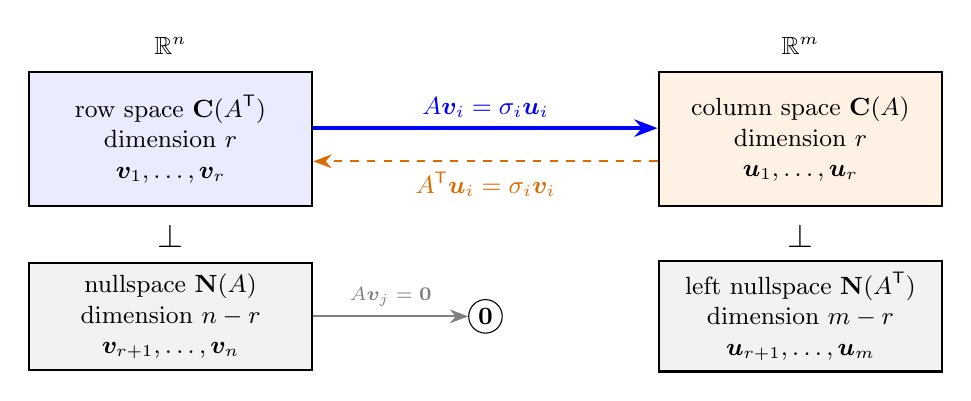
\begin{tikzpicture}[>=Stealth,font=\small,
  sp/.style={draw,thick,fill=#1,minimum width=3.6cm,align=center,inner sep=4pt}]
  \node[sp=blue!8,minimum height=1.7cm] (R) at (0,1.2)
    {row space $\Col{A\T}$\\ dimension $r$\\ $\vb{v}_1,\dots,\vb{v}_r$};
  \node[sp=gray!10,minimum height=1.3cm] (N) at (0,-1.05)
    {nullspace $\Nul{A}$\\ dimension $n-r$\\ $\vb{v}_{r+1},\dots,\vb{v}_n$};
  \node[sp=orange!10,minimum height=1.7cm] (C) at (8,1.2)
    {column space $\Col{A}$\\ dimension $r$\\ $\vb{u}_1,\dots,\vb{u}_r$};
  \node[sp=gray!10,minimum height=1.3cm] (LN) at (8,-1.05)
    {left nullspace $\Nul{A\T}$\\ dimension $m-r$\\ $\vb{u}_{r+1},\dots,\vb{u}_m$};
  \node[above] at (0,2.15) {$\R^n$};
  \node[above] at (8,2.15) {$\R^m$};
  \node[font=\large] at (0,-0.03) {$\perp$};
  \node[font=\large] at (8,-0.03) {$\perp$};
  \draw[->,very thick,blue] ([yshift=4pt]R.east) -- node[above] {$A\vb{v}_i=\sigma_i\vb{u}_i$} ([yshift=4pt]C.west);
  \draw[->,thick,dashed,orange!85!black] ([yshift=-8pt]C.west) -- node[below] {$A\T\vb{u}_i=\sigma_i\vb{v}_i$} ([yshift=-8pt]R.east);
  \node[circle,draw,inner sep=1.5pt] (Z) at (4,-1.05) {$\vb{0}$};
  \draw[->,thick,gray] (N.east) -- node[above,font=\scriptsize] {$A\vb{v}_j=\vb{0}$} (Z);
\end{tikzpicture}
\caption{The SVD chooses orthonormal bases for the four fundamental subspaces so that $A$ acts
diagonally: the row space basis $\vb{v}_i$ goes to $\sigma_i$ times the column space basis $\vb{u}_i$, and the
nullspace basis goes to zero. The left nullspace basis $\vb{u}_{r+1},\dots,\vb{u}_m$ is never reached.}
\label{fig:u33-bigpicture}
\end{figure}

\subsection{Exercises}

\begin{exercise}[Following the ellipse]\label{exr:u33-practice}
For $A=\left[\begin{smallmatrix}6&8\\-4&3\end{smallmatrix}\right]$ of Example~\ref{ex:u33-short}, where does $A$
send $2\vb{v}_1+\vb{v}_2$? Answer once by direct multiplication and once using $A\vb{v}_i=\sigma_i\vb{u}_i$.
\end{exercise}
\begin{solution}
$2\vb{v}_1+\vb{v}_2=(1.2-0.8,\ 1.6+0.6)=(0.4,\,2.2)$. Directly, $A(0.4,2.2)=(2.4+17.6,\ -1.6+6.6)=(20,\,5)$.
With the SVD, $A(2\vb{v}_1+\vb{v}_2)=2\sigma_1\vb{u}_1+\sigma_2\vb{u}_2=2(10,0)+(0,5)=(20,5)$. In the $\vb{v}$-coordinates the
matrix just scales the coordinates $2$ and $1$ by $10$ and $5$.
\end{solution}

\begin{exercise}[The Fibonacci matrix]\label{exr:u33-fib}
Show that the singular values of $A=\left[\begin{smallmatrix}1&1\\1&0\end{smallmatrix}\right]$ are
$\sigma_1=\frac{1+\sqrt5}{2}$ and $\sigma_2=\frac{\sqrt5-1}{2}$. How are they related to the
eigenvalues of $A$?
\end{exercise}
\begin{solution}
$A\T A=AA\T=\left[\begin{smallmatrix}2&1\\1&1\end{smallmatrix}\right]$, with characteristic polynomial
$\lambda^2-3\lambda+1$, so $\sigma_1^2=\frac{3+\sqrt5}{2}$ and $\sigma_2^2=\frac{3-\sqrt5}{2}$. Squaring the
claimed values: $\bigl(\frac{1+\sqrt5}{2}\bigr)^2=\frac{1+2\sqrt5+5}{4}=\frac{3+\sqrt5}{2}$ and
$\bigl(\frac{\sqrt5-1}{2}\bigr)^2=\frac{5-2\sqrt5+1}{4}=\frac{3-\sqrt5}{2}$. Since $A$ is symmetric, its
eigenvalues $\frac{1\pm\sqrt5}{2}$ are real and the singular values are their absolute values; the
negative eigenvalue $\frac{1-\sqrt5}{2}$ becomes $\sigma_2=\frac{\sqrt5-1}{2}$, and its sign moves into
$\vb{u}_2=-\vb{v}_2$.
\end{solution}

\begin{exercise}[Orthogonal columns]\label{exr:u33-orthcols}
Suppose the $n$ columns $\vb{w}_1,\dots,\vb{w}_n$ of $A$ are orthogonal, with lengths $\sigma_1\ge\cdots\ge\sigma_n>0$.
Compute $A\T A$ and find $U$, $\Sigma$, $V$.
\end{exercise}
\begin{solution}
The $(i,j)$ entry of $A\T A$ is $\vb{w}_i\T\vb{w}_j$, so $A\T A=\operatorname{diag}(\sigma_1^2,\dots,\sigma_n^2)$. Its
eigenvectors are the standard basis vectors, so $V=I$ and the singular values are the lengths
$\sigma_i$. Then $\vb{u}_i=A\vb{v}_i/\sigma_i=A\vb{e}_i/\sigma_i=\vb{w}_i/\sigma_i$: the columns of $U$ are the unit
vectors in the column directions (completed by an orthonormal basis of $\Nul{A\T}$ if $m>n$).
\end{solution}

\begin{exercise}[An SVD from scratch]\label{exr:u33-C}
Find the SVD of $C=\left[\begin{smallmatrix}5&5\\-1&7\end{smallmatrix}\right]$.
\end{exercise}
\begin{solution}
$C\T C=\left[\begin{smallmatrix}5&-1\\5&7\end{smallmatrix}\right]\left[\begin{smallmatrix}5&5\\-1&7\end{smallmatrix}\right]
=\left[\begin{smallmatrix}26&18\\18&74\end{smallmatrix}\right]$, with
$\det(C\T C-\lambda I)=\lambda^2-100\lambda+(26\cdot74-324)=\lambda^2-100\lambda+1600=(\lambda-80)(\lambda-20)$.
For $\lambda=80$: $C\T C-80I=\left[\begin{smallmatrix}-54&18\\18&-6\end{smallmatrix}\right]$ gives
$\vb{v}_1=(1,3)/\sqrt{10}$. For $\lambda=20$: $\left[\begin{smallmatrix}6&18\\18&54\end{smallmatrix}\right]$ gives
$\vb{v}_2=(-3,1)/\sqrt{10}$. So $\sigma_1=\sqrt{80}=4\sqrt5$, $\sigma_2=\sqrt{20}=2\sqrt5$. Then
\[
  \vb{u}_1=\frac{C\vb{v}_1}{\sigma_1}=\frac{(20,20)}{\sqrt{10}\cdot4\sqrt5}=\frac{1}{\sqrt2}\begin{bmatrix}1\\1\end{bmatrix},\qquad
  \vb{u}_2=\frac{C\vb{v}_2}{\sigma_2}=\frac{(-10,10)}{\sqrt{10}\cdot2\sqrt5}=\frac{1}{\sqrt2}\begin{bmatrix}-1\\1\end{bmatrix},
\]
\[
  C=\frac{1}{\sqrt2}\begin{bmatrix}1&-1\\1&1\end{bmatrix}
    \begin{bmatrix}4\sqrt5&0\\0&2\sqrt5\end{bmatrix}
    \frac{1}{\sqrt{10}}\begin{bmatrix}1&3\\-3&1\end{bmatrix}.
\]
Check: $|\det C|=|35+5|=40=4\sqrt5\cdot2\sqrt5$.
\end{solution}

% unit: u34
% sources: sources/098-linear-transformations-and-their-matrices.txt, sources/059-lecture-30-linear-transformations-and-their-matrices.txt, sources/221-mit18-06scf11-ses3-6sum-pdf-download-file.txt, sources/060-problem-solving-linear-transformations.txt, sources/222-mit18-06scf11-ses3-6prob-pdf-download-file.txt, sources/223-mit18-06scf11-ses3-6sol-pdf-download-file.txt
\section{Linear transformations and their matrices}\label{sec:u34}

Many linear algebra courses begin where this unit begins: with linear transformations,
described without coordinates. A projection onto a line or a rotation of the plane makes sense
before anyone writes down a matrix, and some people (physicists especially) prefer to think
that way, about the whole space at once. But as soon as we want to compute, we choose a basis,
coordinates appear, and every linear transformation becomes a matrix. Everything we have
learned about matrices (nullspaces, determinants, eigenvalues) then applies. This unit
explains that passage from transformation to matrix, and why the eigenvector basis gives the
best matrix of all.

\subsection{Linearity without coordinates}

\begin{definition}[Linear transformation]\label{def:u34-linear}
Let $V$ and $W$ be vector spaces. A \emph{transformation} (or map) $T\colon V\to W$ assigns an
output $T(\vb{v})\in W$ to every input $\vb{v}\in V$. It is \emph{linear} if, for all vectors
$\vb{v},\vb{w}$ and all scalars $c$,
\[
  T(\vb{v}+\vb{w})=T(\vb{v})+T(\vb{w})\qquad\text{and}\qquad T(c\vb{v})=c\,T(\vb{v}).
\]
Equivalently, $T(c\vb{v}+d\vb{w})=c\,T(\vb{v})+d\,T(\vb{w})$: $T$ respects the two operations on vectors,
addition and scalar multiplication, and so respects every linear combination.
\end{definition}

\begin{proposition}[Zero goes to zero]\label{prop:u34-zero}
Every linear transformation satisfies $T(\vb{0})=\vb{0}$.
\end{proposition}
\begin{proof}
Take $c=0$ in $T(c\vb{v})=cT(\vb{v})$: $T(\vb{0})=T(0\vb{v})=0\,T(\vb{v})=\vb{0}$.
\end{proof}

\emph{Examples.}
\begin{itemize}
  \item \emph{Projection} $T\colon\R^2\to\R^2$ onto a fixed line through the origin. Doubling
        $\vb{v}$ doubles its projection, reversing $\vb{v}$ reverses it, and the projection of a sum is the
        sum of the projections.
  \item \emph{Rotation} of the plane by $45^\circ$ about the origin. Rotating $\vb{v}+\vb{w}$ gives the
        same result as rotating $\vb{v}$ and $\vb{w}$ and then adding: the whole parallelogram rotates.
  \item \emph{Multiplication by a matrix}, $T(\vb{v})=A\vb{v}$. This is linear because
        $A(\vb{v}+\vb{w})=A\vb{v}+A\vb{w}$ and $A(c\vb{v})=c\,A\vb{v}$. Any $2\times3$ matrix gives a linear
        $T\colon\R^3\to\R^2$.
  \item \emph{Differentiation}, $T(f)=f'$, on a space of functions: $(f+g)'=f'+g'$ and $(cf)'=cf'$.
        This is why we can differentiate any combination of $\sin x$, $\cos x$, $e^x$, \dots{} once we
        know the derivatives of a short list.
\end{itemize}

\emph{Non-examples.}
\begin{itemize}
  \item \emph{Shift the whole plane}, $T(\vb{v})=\vb{v}+\vb{v}_0$ with a fixed $\vb{v}_0\ne\vb{0}$. Then
        $T(2\vb{v})=2\vb{v}+\vb{v}_0$ but $2T(\vb{v})=2\vb{v}+2\vb{v}_0$, and $T(\vb{0})=\vb{v}_0\ne\vb{0}$.
  \item \emph{Length}, $T(\vb{v})=\|\vb{v}\|$ from $\R^3$ to $\R$. It does send $\vb{0}$ to $0$ and doubles
        when $\vb{v}$ doubles, but $T(-2\vb{v})=2\|\vb{v}\|\ne-2\|\vb{v}\|$.
\end{itemize}

The advantage of the coordinate-free view is the big picture. Instead of following one vector,
watch what $T$ does to a whole figure, such as the outline of a house (Figure~\ref{fig:u34-house}).
The matrix $\left[\begin{smallmatrix}1&0\\0&-1\end{smallmatrix}\right]$ keeps each $x$-component and
reverses each $y$-component, so it reflects the house across the $x$-axis and turns it upside
down; the rotation turns it without distortion; the shift moves it, origin and all, which is how
we see at once that it is not linear.

\begin{figure}[ht]\centering
\begin{tikzpicture}[>=Stealth,scale=0.85,
  house/.pic={
    \draw[thick,fill=blue!10] (0,0) -- (1,0) -- (1,1) -- (0.5,1.55) -- (0,1) -- cycle;
    \draw[thick,fill=orange!40] (0.38,0) -- (0.38,0.5) -- (0.62,0.5) -- (0.62,0);
    \fill[red!70!black] (0.5,1.55) circle (1.6pt);
  }]
  \begin{scope}
    \draw[->,gray] (-1.3,0) -- (1.6,0); \draw[->,gray] (0,-1.7) -- (0,1.9);
    \pic at (0,0) {house};
    \node[font=\small] at (0.15,-2.15) {input};
  \end{scope}
  \begin{scope}[xshift=3.9cm]
    \draw[->,gray] (-1.3,0) -- (1.6,0); \draw[->,gray] (0,-1.7) -- (0,1.9);
    \pic[rotate=45] at (0,0) {house};
    \node[font=\small] at (0.15,-2.15) {rotation by $45^\circ$};
  \end{scope}
  \begin{scope}[xshift=7.8cm]
    \draw[->,gray] (-1.3,0) -- (1.6,0); \draw[->,gray] (0,-1.7) -- (0,1.9);
    \pic[yscale=-1] at (0,0) {house};
    \node[font=\small] at (0.15,-2.15) {$\left[\begin{smallmatrix}1&0\\0&-1\end{smallmatrix}\right]$: reflection};
  \end{scope}
  \begin{scope}[xshift=11.7cm]
    \draw[->,gray] (-1.3,0) -- (1.6,0); \draw[->,gray] (0,-1.7) -- (0,1.9);
    \pic at (0.6,-1.2) {house};
    \draw[->,thick,red!70!black] (0,0) -- (0.6,-1.2) node[pos=0.45,left,font=\scriptsize] {$\vb{v}_0$};
    \node[font=\small] at (0.15,-2.15) {shift: not linear};
  \end{scope}
\end{tikzpicture}
\caption{A linear transformation acts on the whole plane at once; following a house shows the
effect. Rotation and the reflection matrix keep the origin fixed and carry straight lines to
straight lines and parallelograms to parallelograms. The shift $T(\vb{v})=\vb{v}+\vb{v}_0$ moves the corner at
the origin to $\vb{v}_0$, violating $T(\vb{0})=\vb{0}$.}
\label{fig:u34-house}
\end{figure}

\subsection{A basis determines everything}

How much must we be told about a linear $T$ to know $T(\vb{v})$ for every input? Knowing $T(\vb{v}_1)$
gives $T(c\vb{v}_1)=cT(\vb{v}_1)$ on a whole line. Knowing $T(\vb{v}_1)$ and $T(\vb{v}_2)$ for independent
$\vb{v}_1,\vb{v}_2$ gives $T(c\vb{v}_1+d\vb{v}_2)$ on a whole plane. (If $\vb{v}_2$ were $6\vb{v}_1$, then $T(\vb{v}_2)$
would carry no new information.) A basis is enough.

\begin{theorem}[Linear maps are determined by a basis]\label{thm:u34-basis}
Let $\vb{v}_1,\dots,\vb{v}_n$ be a basis of $V$. If $T$ is linear, then for every $\vb{v}=c_1\vb{v}_1+\cdots+c_n\vb{v}_n$,
\[
  T(\vb{v})=c_1T(\vb{v}_1)+c_2T(\vb{v}_2)+\cdots+c_nT(\vb{v}_n).
\]
So $T$ is completely known once $T(\vb{v}_1),\dots,T(\vb{v}_n)$ are known.
\end{theorem}
\begin{proof}
Because the $\vb{v}_i$ span $V$, every $\vb{v}$ is such a combination; linearity, applied repeatedly to
the combination, gives the formula.
\end{proof}

\begin{definition}[Coordinates]\label{def:u34-coordinates}
If $\vb{v}_1,\dots,\vb{v}_n$ is a basis of $V$ and $\vb{v}=c_1\vb{v}_1+\cdots+c_n\vb{v}_n$, the numbers
$(c_1,\dots,c_n)$ are the \emph{coordinates} of $\vb{v}$ in this basis. They are unique: if also
$\vb{v}=\sum d_i\vb{v}_i$, then $\sum(c_i-d_i)\vb{v}_i=\vb{0}$, and independence forces every $c_i=d_i$.
\end{definition}

Coordinates come from a basis. When someone writes $\vb{v}=(3,2,4)$ we silently assume the
standard basis, $\vb{v}=3\vb{e}_1+2\vb{e}_2+4\vb{e}_3$, and then the coordinates are the components. But
another basis, for example the eigenvectors of some matrix, gives the same vector different
coordinates.

\subsection{The matrix of a transformation}

To turn $T\colon V\to W$ into a matrix we choose \emph{two} bases: an input basis $\vb{v}_1,\dots,\vb{v}_n$
of $V$ and an output basis $\vb{w}_1,\dots,\vb{w}_m$ of $W$. The matrix will take the input coordinates
to the output coordinates.

\begin{definition}[Matrix of \texorpdfstring{$T$}{T} in chosen bases]\label{def:u34-matrix}
Expand the output of each input basis vector in the output basis:
\[
  T(\vb{v}_j)=a_{1j}\vb{w}_1+a_{2j}\vb{w}_2+\cdots+a_{mj}\vb{w}_m\qquad(j=1,\dots,n).
\]
The $m\times n$ matrix $A=(a_{ij})$ is the \emph{matrix of $T$} in these bases: column $j$ holds the
output coordinates of $T(\vb{v}_j)$.
\end{definition}

\begin{theorem}[The matrix does what \texorpdfstring{$T$}{T} does]\label{thm:u34-matrix}
If $\vb{v}$ has input coordinates $\vb{c}=(c_1,\dots,c_n)$, then $T(\vb{v})$ has output coordinates $A\vb{c}$.
\end{theorem}
\begin{proof}
By Theorem~\ref{thm:u34-basis} and the definition of the columns,
\[
  T(\vb{v})=\sum_{j}c_jT(\vb{v}_j)=\sum_{j}c_j\sum_{i}a_{ij}\vb{w}_i=\sum_{i}\Bigl(\sum_{j}a_{ij}c_j\Bigr)\vb{w}_i ,
\]
and $\sum_ja_{ij}c_j$ is component $i$ of $A\vb{c}$. As a sanity check, the input coordinates
$(1,0,\dots,0)$ describe $\vb{v}_1$, and $A$ times them is column~1, the coordinates of $T(\vb{v}_1)$.
\end{proof}

\begin{example}[One projection, two matrices]\label{ex:u34-projection}
Let $T$ project $\R^2$ onto the $45^\circ$ line, using the same basis for inputs and outputs.

\emph{A good basis.} Take $\vb{v}_1=(1,1)/\sqrt2$ on the line and $\vb{v}_2=(-1,1)/\sqrt2$ perpendicular to
it. The projection leaves $\vb{v}_1$ alone and kills $\vb{v}_2$: $T(\vb{v}_1)=1\vb{v}_1+0\vb{v}_2$ and
$T(\vb{v}_2)=0\vb{v}_1+0\vb{v}_2$. So
\[
  A=\begin{bmatrix}1&0\\0&0\end{bmatrix},\qquad A\begin{bmatrix}c_1\\c_2\end{bmatrix}=\begin{bmatrix}c_1\\0\end{bmatrix}.
\]
These basis vectors are the eigenvectors of the projection (eigenvalues $1$ and $0$), and the
matrix came out as the diagonal eigenvalue matrix $\Lambda$.

\emph{The standard basis.} With $\vb{v}_1=\vb{w}_1=(1,0)$ and $\vb{v}_2=\vb{w}_2=(0,1)$: the projection of $(1,0)$
onto the line is $(\tfrac12,\tfrac12)$, and so is the projection of $(0,1)$. So
\[
  P=\begin{bmatrix}\tfrac12&\tfrac12\\\tfrac12&\tfrac12\end{bmatrix}=\frac{\vb{a}\vb{a}\T}{\vb{a}\T\vb{a}}\quad\text{with }\vb{a}=(1,1),
\]
the projection matrix of Section~\ref{sec:u17}. It is symmetric with $P^2=P$, but those facts are
obvious only in the eigenvector basis, where the matrix is diagonal. The course has mostly used
the handiest basis; the best basis is the eigenvector basis.
\end{example}

\begin{example}[Differentiation as a matrix]\label{ex:u34-derivative}
Let $T=\frac{d}{dx}$ take the quadratics $c_1+c_2x+c_3x^2$ (input basis $1,x,x^2$) to the linear
polynomials (output basis $1,x$): $T(c_1+c_2x+c_3x^2)=c_2+2c_3x$. Column by column,
$T(1)=0$, $T(x)=1$, $T(x^2)=2x$, so
\[
  A=\begin{bmatrix}0&1&0\\0&0&2\end{bmatrix},\qquad
  A\begin{bmatrix}c_1\\c_2\\c_3\end{bmatrix}=\begin{bmatrix}c_2\\2c_3\end{bmatrix}.
\]
For instance $p(x)=5+3x-4x^2$ has coordinates $(5,3,-4)$, and $A(5,3,-4)=(3,-8)$, the coordinates
of $p'(x)=3-8x$. The $2\times3$ shape reflects a three-dimensional input space and a
two-dimensional output space; the nullspace of $A$, spanned by $(1,0,0)$, is the constant
polynomials, whose derivative is zero.
\end{example}

\begin{example}[The transpose as a linear map]\label{ex:u34-transpose}
On the four-dimensional space of $2\times2$ matrices let $T(X)=X\T$. It is linear:
$(X+Y)\T=X\T+Y\T$ and $(cX)\T=cX\T$. Applying it twice gives back $X$, so $T^2=I$ and $T^{-1}=T$.
\begin{itemize}
  \item In the standard basis $\vb{v}_1=\left[\begin{smallmatrix}1&0\\0&0\end{smallmatrix}\right]$,
        $\vb{v}_2=\left[\begin{smallmatrix}0&1\\0&0\end{smallmatrix}\right]$,
        $\vb{v}_3=\left[\begin{smallmatrix}0&0\\1&0\end{smallmatrix}\right]$,
        $\vb{v}_4=\left[\begin{smallmatrix}0&0\\0&1\end{smallmatrix}\right]$ we have
        $T(\vb{v}_1)=\vb{v}_1$, $T(\vb{v}_2)=\vb{v}_3$, $T(\vb{v}_3)=\vb{v}_2$, $T(\vb{v}_4)=\vb{v}_4$, so the matrix is the
        permutation
        \[
          M_T=\begin{bmatrix}1&0&0&0\\0&0&1&0\\0&1&0&0\\0&0&0&1\end{bmatrix}.
        \]
        Check: $\left[\begin{smallmatrix}1&2\\3&4\end{smallmatrix}\right]$ has coordinates $(1,2,3,4)$ and
        $M_T(1,2,3,4)=(1,3,2,4)$, the coordinates of its transpose
        $\left[\begin{smallmatrix}1&3\\2&4\end{smallmatrix}\right]$.
  \item In the basis $\vb{w}_1=\left[\begin{smallmatrix}1&0\\0&0\end{smallmatrix}\right]$,
        $\vb{w}_2=\left[\begin{smallmatrix}0&1\\1&0\end{smallmatrix}\right]$,
        $\vb{w}_3=\left[\begin{smallmatrix}0&0\\0&1\end{smallmatrix}\right]$,
        $\vb{w}_4=\left[\begin{smallmatrix}0&1\\-1&0\end{smallmatrix}\right]$, the first three are symmetric and the
        last is antisymmetric: $T(\vb{w}_i)=\vb{w}_i$ for $i\le3$ and $T(\vb{w}_4)=-\vb{w}_4$. The matrix is
        $\operatorname{diag}(1,1,1,-1)$. These $\vb{w}$'s are eigenvectors of $T$: the symmetric matrices
        are its eigenspace for $\lambda=1$ and the antisymmetric ones for $\lambda=-1$.
\end{itemize}
\end{example}

\begin{trap}
A matrix of $T$ means nothing until both bases are named, and the same $T$ has many matrices
(compare the two projection matrices above). Also, the coordinate vector of an output must be
taken in the \emph{output} basis: for $\frac{d}{dx}$, the column for $x^2$ is $(0,2)$ because
$2x=0\cdot1+2\cdot x$, not $(0,0,2)$ or $(2,0)$.
\end{trap}

\subsection{Products of transformations are products of matrices}

If $T_1\colon U\to V$ and $T_2\colon V\to W$ are linear, so is the composition $T_2\circ T_1$
($\vb{u}\mapsto T_2(T_1(\vb{u}))$). Matrix multiplication was defined to match.

\begin{proposition}[Composition and inverses]\label{prop:u34-composition}
Fix bases of $U$, $V$, $W$. If $T_1$ has matrix $A_1$ and $T_2$ has matrix $A_2$, then
$T_2\circ T_1$ has matrix $A_2A_1$. If $T\colon V\to V$ is invertible with matrix $A$ (same basis in
and out), then $T^{-1}$ has matrix $A^{-1}$.
\end{proposition}
\begin{proof}
Let $\vb{u}$ have coordinates $\vb{c}$. By Theorem~\ref{thm:u34-matrix}, $T_1(\vb{u})$ has coordinates $A_1\vb{c}$,
and then $T_2(T_1(\vb{u}))$ has coordinates $A_2(A_1\vb{c})=(A_2A_1)\vb{c}$; a matrix that does this for every
$\vb{c}$ is the matrix of the composition (its columns come from $\vb{c}=\vb{e}_j$). For the inverse,
$T^{-1}\circ T$ is the identity, whose matrix is $I$, so the matrix $B$ of $T^{-1}$ satisfies $BA=I$.
\end{proof}

\begin{example}[The second derivative]\label{ex:u34-second}
Follow $\frac{d}{dx}$ from quadratics to linear polynomials (matrix $A_1$ above) by
$\frac{d}{dx}$ from linear polynomials (basis $1,x$) to constants (basis $1$), whose matrix is
$A_2=\begin{bmatrix}0&1\end{bmatrix}$. The product
\[
  A_2A_1=\begin{bmatrix}0&1\end{bmatrix}\begin{bmatrix}0&1&0\\0&0&2\end{bmatrix}=\begin{bmatrix}0&0&2\end{bmatrix}
\]
sends $(c_1,c_2,c_3)$ to $2c_3$, and indeed $\frac{d^2}{dx^2}(c_1+c_2x+c_3x^2)=2c_3$.
\end{example}

\subsection{Exercises}

\begin{exercise}[Doubling every distance]\label{exr:u34-polar}
In polar coordinates let $T(r,\theta)=(2r,\theta)$: $T$ doubles the distance from the origin and keeps
the direction.
\begin{enumerate}[(a)]
  \item Is $T$ linear?
  \item Describe $T$ in Cartesian coordinates and check that it doubles lengths.
  \item Find its matrix in the standard basis.
\end{enumerate}
\end{exercise}
\begin{solution}
\begin{enumerate}[(a)]
  \item Yes. As a map of vectors, $T(\vb{v})=2\vb{v}$, so $T(\vb{v}_1+\vb{v}_2)=2\vb{v}_1+2\vb{v}_2=T(\vb{v}_1)+T(\vb{v}_2)$ and
        $T(c\vb{v})=2c\vb{v}=cT(\vb{v})$.
  \item $T(x,y)=(2x,2y)$, and $\|(2x,2y)\|=\sqrt{4x^2+4y^2}=2\sqrt{x^2+y^2}=2\|(x,y)\|$.
  \item $T(1,0)=(2,0)$ and $T(0,1)=(0,2)$, so the matrix is
        $\left[\begin{smallmatrix}2&0\\0&2\end{smallmatrix}\right]=2I$.
\end{enumerate}
\end{solution}

\begin{exercise}[Fixing zero is not enough]\label{exr:u34-nonlinear}
Find a transformation of $\R^2$ with $T(\vb{0})=\vb{0}$ that is not linear.
\end{exercise}
\begin{solution}
One option acts differently on different parts of the plane: $T(x,y)=(|x|,|y|)$. Then
$T\bigl((1,1)+(1,-1)\bigr)=T(2,0)=(2,0)$, but $T(1,1)+T(1,-1)=(1,1)+(1,1)=(2,2)$. Another uses a
nonlinear formula: $T(x,y)=(x,y^2)$ gives $T(c(x,y))=(cx,c^2y^2)$, which differs from
$cT(x,y)=(cx,cy^2)$ when $c\ne0,1$ and $y\ne0$. Both send $\vb{0}$ to $\vb{0}$, so $T(\vb{0})=\vb{0}$ is a
necessary condition for linearity, not a sufficient one.
\end{solution}

\begin{exercise}[Rotations compose by adding angles]\label{exr:u34-rotation}
Find the matrix $R_\theta$ of rotation by $\theta$ in the standard basis, and use
Proposition~\ref{prop:u34-composition} to show $R_\theta R_\varphi=R_{\theta+\varphi}$. What is $R_\theta^{-1}$?
\end{exercise}
\begin{solution}
Rotating $(1,0)$ gives $(\cos\theta,\sin\theta)$ and rotating $(0,1)$ gives $(-\sin\theta,\cos\theta)$, so
\[
  R_\theta=\begin{bmatrix}\cos\theta&-\sin\theta\\\sin\theta&\cos\theta\end{bmatrix}.
\]
Rotating by $\varphi$ and
then by $\theta$ is rotation by $\theta+\varphi$, so the product of the matrices must be $R_{\theta+\varphi}$.
Multiplying out confirms it: the $(1,1)$ entry is $\cos\theta\cos\varphi-\sin\theta\sin\varphi=\cos(\theta+\varphi)$ and
the $(2,1)$ entry is $\sin\theta\cos\varphi+\cos\theta\sin\varphi=\sin(\theta+\varphi)$: the matrix product contains the
addition formulas of trigonometry. The inverse rotation is $R_{-\theta}=R_\theta\T$.
\end{solution}

\begin{exercise}[Integration undoes differentiation, on one side]\label{exr:u34-integral}
Let $S$ take linear polynomials $c_1+c_2x$ to quadratics by $S(p)=\int_0^xp(t)\,dt$, and let $D=\frac{d}{dx}$
take quadratics to linear polynomials (bases $1,x$ and $1,x,x^2$). Find the matrices of $S$ and $D$, and
compute $DS$ and $SD$. Interpret.
\end{exercise}
\begin{solution}
$S(1)=x$ and $S(x)=\tfrac12x^2$, so $S$ has matrix $\left[\begin{smallmatrix}0&0\\1&0\\0&1/2\end{smallmatrix}\right]$; $D$
has matrix $\left[\begin{smallmatrix}0&1&0\\0&0&2\end{smallmatrix}\right]$ (Example~\ref{ex:u34-derivative}).
Then $DS=\left[\begin{smallmatrix}1&0\\0&1\end{smallmatrix}\right]=I$: differentiating an integral returns the
original function. But $SD=\left[\begin{smallmatrix}0&0&0\\0&1&0\\0&0&1\end{smallmatrix}\right]\ne I$: integrating a
derivative loses the constant term $c_1$. So $S$ is a right inverse of $D$ but not a left inverse,
a theme of Section~\ref{sec:u36}.
\end{solution}

% unit: u35
% sources: sources/076-change-of-basis-image-compression.txt, sources/061-lecture-31-change-of-basis-image-compression.txt, sources/224-mit18-06scf11-ses3-7sum-pdf-download-file.txt, sources/062-problem-solving-change-of-basis.txt, sources/225-mit18-06scf11-ses3-7prob-pdf-download-file.txt, sources/226-mit18-06scf11-ses3-7sol-pdf-download-file.txt
\section{Change of basis; image compression}\label{sec:u35}

Section~\ref{sec:u34} showed that a linear transformation becomes a matrix once a basis is
chosen, and that a better basis gives a better matrix. This unit makes the change from one
basis to another explicit, for vectors (new coordinates) and for transformations (a new,
similar matrix). It starts with the application where the choice of basis is worth billions:
compressing images and video. Recording an image pixel by pixel uses the standard basis, which
is a poor basis for real pictures; switching to a Fourier or wavelet basis lets us keep a few
large coefficients and throw the rest away.

\subsection{Images are vectors, and the standard basis is poor}

A black-and-white image of $512\times512$ pixels records a gray level at every pixel, usually an
integer from $0$ to $255$ (eight bits). The image is therefore a vector $\vb{x}\in\R^n$ with
$n=512^2=262{,}144$ components; a color image needs three times as many. Sending each frame of a
video pixel by pixel would overload any channel.

Giving the value of each pixel is using the standard basis $\vb{e}_1,\dots,\vb{e}_n$: the coefficient of
$\vb{e}_i$ is pixel $i$. This ignores the most important feature of real images, that neighboring
pixels have nearly the same gray level. Before the lecture starts, the camera sees a blank
blackboard: every pixel is (almost) the same. Pixel by pixel that image still costs $n$ numbers.
In a basis that contains the vector of all ones, it costs \emph{one} coefficient. Other useful
basis vectors are the checkerboard $(1,-1,1,-1,\dots)$ and the half-and-half vector
$(1,\dots,1,-1,\dots,-1)$, an image bright on the left and dark on the right. Which basis is best
depends on the signal: the best basis for algebra lectures may not be the best for action films.

\subsection{Transform, threshold, reconstruct}

Lossy compression has three steps, only one of which loses information:
\[
  \underbrace{\vb{x}}_{\text{pixels}}
  \;\xrightarrow{\ \text{change basis (lossless)}\ }\;
  \underbrace{\vb{c}}_{\text{coefficients}}
  \;\xrightarrow{\ \text{threshold (lossy)}\ }\;
  \underbrace{\hat{\vb{c}}}_{\text{many zeros}}
  \;\xrightarrow{\ \text{reconstruct}\ }\;
  \hat{\vb{x}}=\sum_i\hat c_i\vb{w}_i .
\]
The change of basis writes $\vb{x}=c_1\vb{w}_1+\cdots+c_n\vb{w}_n$ in a new basis. \emph{Thresholding} sets
to zero every coefficient below a chosen size, small enough that the eye can hardly see the
difference. A smooth image has a large coefficient on the constant vector (zero frequency) and
very little of the fast-alternating, high-frequency vectors. If $64$ coefficients shrink to $3$,
that is compression by a factor of about $21$.

The JPEG standard (Joint Photographic Experts Group) cuts the $512\times512$ image into $8\times8$
blocks of $64$ pixels and changes basis separately in each block, using cosines: the real parts
of the Fourier vectors of Section~\ref{sec:u30}. Video adds a time dimension. Consecutive frames
are very close, so a good coder predicts each frame from the previous one and encodes only the
small correction. In space or in time, compression exploits the same fact: signals change
smoothly, so neighboring values predict each other.

\subsection{The Haar wavelet basis}

The main competitor to the Fourier basis is a \emph{wavelet} basis. The simplest wavelets, Haar's,
in $\R^8$ are the columns $\vb{w}_1,\dots,\vb{w}_8$ of
\[
  W=\begin{bmatrix*}[r]
  1&1&1&0&1&0&0&0\\
  1&1&1&0&-1&0&0&0\\
  1&1&-1&0&0&1&0&0\\
  1&1&-1&0&0&-1&0&0\\
  1&-1&0&1&0&0&1&0\\
  1&-1&0&1&0&0&-1&0\\
  1&-1&0&-1&0&0&0&1\\
  1&-1&0&-1&0&0&0&-1
  \end{bmatrix*}:
\]
the constant vector, one vector that is $+1$ on the first half and $-1$ on the second, two
that do the same on each half, and four that do it on each quarter
(Figure~\ref{fig:u35-haar}). Every entry is $0$ or $\pm1$, so multiplying by $W$ needs only
additions and subtractions. JPEG2000 uses smoother wavelets built on the same idea.

\begin{figure}[ht]\centering
\begin{tikzpicture}[x=0.25cm,y=0.36cm]
  \foreach \vals [count=\i from 0] in
    {{1,1,1,1,1,1,1,1},{1,1,1,1,-1,-1,-1,-1},{1,1,-1,-1,0,0,0,0},{0,0,0,0,1,1,-1,-1},
     {1,-1,0,0,0,0,0,0},{0,0,1,-1,0,0,0,0},{0,0,0,0,1,-1,0,0},{0,0,0,0,0,0,1,-1}} {
    \pgfmathtruncatemacro{\col}{mod(\i,4)}
    \pgfmathtruncatemacro{\row}{int(\i/4)}
    \pgfmathtruncatemacro{\num}{\i+1}
    \begin{scope}[xshift={\col*3.4cm},yshift={-\row*1.55cm}]
      \foreach \h [count=\k from 0] in \vals {
        \fill[blue!55] (\k+0.12,0) rectangle (\k+0.88,\h);
      }
      \draw[gray] (-0.3,0) -- (8.3,0);
      \draw[gray,very thin] (-0.3,1) -- (-0.1,1) (-0.3,-1) -- (-0.1,-1);
      \node[font=\small,anchor=east] at (-0.4,0) {$\vb{w}_{\num}$};
    \end{scope}
  }
\end{tikzpicture}
\caption{The eight Haar wavelets in $\R^8$, drawn as bar charts of their entries ($+1$ up, $-1$
down). Top row: the constant vector and the coarse wavelets on halves and quarters of the
signal. Bottom row: the finest wavelets, each a single $+1,-1$ pair. Their sum
$\vb{w}_5+\vb{w}_6+\vb{w}_7+\vb{w}_8=(1,-1,1,-1,1,-1,1,-1)$ is the fastest-oscillating Fourier vector.}
\label{fig:u35-haar}
\end{figure}

Finding the coefficients of $\vb{x}$ means solving $\vb{x}=W\vb{c}$, so $\vb{c}=W^{-1}\vb{x}$. The Haar vectors make
this easy because they are orthogonal: any two of them overlap where one is constant, and there
the other has as many $+1$'s as $-1$'s, so the dot product is zero.

\begin{proposition}[Coefficients in an orthogonal basis]\label{prop:u35-coeffs}
If $\vb{w}_1,\dots,\vb{w}_n$ is an orthogonal basis of $\R^n$ and $\vb{x}=\sum c_j\vb{w}_j$, then
\[
  c_i=\frac{\vb{w}_i\T\vb{x}}{\vb{w}_i\T\vb{w}_i}.
\]
In matrix form $W\T W=D$ is diagonal and $W^{-1}=D^{-1}W\T$. If the basis is orthonormal, $W^{-1}=W\T$.
\end{proposition}
\begin{proof}
Take the dot product of $\vb{x}=\sum_jc_j\vb{w}_j$ with $\vb{w}_i$. Every term with $j\ne i$ vanishes, leaving
$\vb{w}_i\T\vb{x}=c_i\,\vb{w}_i\T\vb{w}_i$. For the matrix form, the $(i,j)$ entry of $W\T W$ is $\vb{w}_i\T\vb{w}_j$, which is
zero off the diagonal; so $(D^{-1}W\T)W=I$.
\end{proof}

For the Haar basis $\vb{w}_i\T\vb{w}_i$ is $8,8,4,4,2,2,2,2$. Dividing each $\vb{w}_i$ by its length $\sqrt8$,
$\sqrt8$, $2$, $2$, $\sqrt2$, $\sqrt2$, $\sqrt2$, $\sqrt2$ makes $W$ orthogonal, with $W^{-1}=W\T$.

\begin{example}[Compressing eight pixels]\label{ex:u35-compress}
One row of an image has gray levels
\[
  \vb{p}=(100,\,102,\,104,\,106,\,60,\,60,\,62,\,62):
\]
a bright region with a gentle ramp next to a dark region. Using
Proposition~\ref{prop:u35-coeffs}, with $\vb{w}_i\T\vb{w}_i=8,8,4,4,2,2,2,2$:
\begin{align*}
  c_1&=\tfrac18(100+102+104+106+60+60+62+62)=\tfrac{656}{8}=82,\\
  c_2&=\tfrac18\bigl((100+102+104+106)-(60+60+62+62)\bigr)=\tfrac{412-244}{8}=21,\\
  c_3&=\tfrac14\bigl((100+102)-(104+106)\bigr)=-2,\qquad
  c_4=\tfrac14\bigl((60+60)-(62+62)\bigr)=-1,\\
  c_5&=\tfrac12(100-102)=-1,\quad c_6=\tfrac12(104-106)=-1,\quad
  c_7=\tfrac12(60-60)=0,\quad c_8=\tfrac12(62-62)=0 .
\end{align*}
So $\vb{c}=(82,21,-2,-1,-1,-1,0,0)$: the average gray level, the bright/dark contrast, and small
details. \emph{Threshold}: drop every coefficient with $|c_i|\le1$, keeping $\hat{\vb{c}}=(82,21,-2,0,0,0,0,0)$.
\emph{Reconstruct}:
\[
  \hat{\vb{x}}=82\vb{w}_1+21\vb{w}_2-2\vb{w}_3=(101,101,105,105,61,61,61,61).
\]
The error $\vb{p}-\hat{\vb{x}}=(-1,1,-1,1,-1,-1,1,1)$ is at most one gray level out of $255$, invisible,
and three numbers replace eight. A harsher threshold keeping only $c_1$ and $c_2$ gives
$82\vb{w}_1+21\vb{w}_2=(103,103,103,103,61,61,61,61)$, with errors up to $3$
(Figure~\ref{fig:u35-signal}). Had we kept
three \emph{pixels} instead, the other five would be lost entirely.
\end{example}

\begin{figure}[ht]\centering
\begin{tikzpicture}[x=0.9cm,y=0.05cm,>=Stealth]
  \begin{scope}[yshift=-2.5cm]
    \draw[->,gray] (0,50) -- (8.4,50) node[right,font=\small] {pixel};
    \draw[->,gray] (0,50) -- (0,115);
    \foreach \v in {60,80,100} {
      \draw[gray] (-0.08,\v) -- (0.08,\v) node[left=2pt,font=\scriptsize,black] {$\v$};
    }
    \foreach \k in {1,...,8} \node[font=\scriptsize,below] at (\k-0.5,50) {$\k$};
    \draw[thick,dashed,blue] (0,103) -- (4,103) -- (4,61) -- (8,61);
    \draw[very thick,red!75!black] (0,101) -- (2,101) -- (2,105) -- (4,105) -- (4,61) -- (8,61);
    \foreach \x/\v in {0.5/100,1.5/102,2.5/104,3.5/106,4.5/60,5.5/60,6.5/62,7.5/62}
      \fill (\x,\v) circle (2.2pt);
    \node[font=\scriptsize,anchor=west] at (8.6,106) {$\bullet$ pixels $\vb{p}$};
    \node[font=\scriptsize,anchor=west,red!75!black] at (8.6,96) {3 coefficients};
    \node[font=\scriptsize,anchor=west,blue] at (8.6,86) {2 coefficients};
  \end{scope}
\end{tikzpicture}
\caption{The pixel row of Example~\ref{ex:u35-compress} (dots) and its reconstructions from the
largest Haar coefficients. Three coefficients, $82\vb{w}_1+21\vb{w}_2-2\vb{w}_3$ (solid), miss no pixel by
more than one gray level; two coefficients (dashed) keep the bright/dark split but flatten the
ramp.}
\label{fig:u35-signal}
\end{figure}

What makes a basis good for compression? Two properties, and the competition between bases
is about both:
\begin{enumerate}
  \item \emph{Fast}: multiplying by $W$ and by $W^{-1}$ must be cheap. The Fourier basis has the FFT
        (Section~\ref{sec:u30}); wavelets have a fast wavelet transform; orthonormal bases have
        $W^{-1}=W\T$. The fastest choice of all is to change nothing, the standard basis, which fails
        the second test.
  \item \emph{Good compression}: a few basis vectors should come close to the signal, so that most
        coefficients are small and can be set to zero.
\end{enumerate}
The ideal basis would be the eigenvectors of a matrix built from the image itself, but finding
them costs far more than the savings; Fourier and wavelet bases are cheap and close.

\subsection{Change of basis for vectors and for transformations}

\emph{Vectors.} Let the columns of $W$ be new basis vectors $\vb{w}_1,\dots,\vb{w}_n$ of $\R^n$. A vector with
standard coordinates $\vb{x}$ has new coordinates $\vb{c}$ related by
\[
  \vb{x}=W\vb{c},\qquad \vb{c}=W^{-1}\vb{x}.
\]

\emph{Transformations.} Now let $T\colon V\to V$ be linear and use the same basis for inputs and
outputs. In an old basis $\vb{v}_1,\dots,\vb{v}_n$ it has a matrix $A$, in a new basis $\vb{w}_1,\dots,\vb{w}_n$ a
matrix $B$. The same transformation should give closely related matrices, and it does.

\begin{theorem}[Changing basis gives a similar matrix]\label{thm:u35-similar}
Let $M$ be the matrix whose column $j$ holds the old coordinates of the new basis vector $\vb{w}_j$.
Then for every vector, $(\text{old coordinates})=M\,(\text{new coordinates})$, and
\[
  B=M^{-1}AM .
\]
\end{theorem}
\begin{proof}
If $\vb{x}=\sum_jd_j\vb{w}_j$, substituting $\vb{w}_j=\sum_iM_{ij}\vb{v}_i$ gives
$\vb{x}=\sum_i\bigl(\sum_jM_{ij}d_j\bigr)\vb{v}_i$, so the old coordinates are $M\vb{d}$. Since $M$ converts
coordinates of a basis into coordinates of a basis, it is invertible. Now follow
Figure~\ref{fig:u35-diagram}: start with new coordinates $\vb{d}$ of $\vb{x}$; $M\vb{d}$ are its old coordinates;
$AM\vb{d}$ are the old coordinates of $T(\vb{x})$ (Section~\ref{sec:u34}); $M^{-1}AM\vb{d}$ are the new coordinates
of $T(\vb{x})$. A matrix that turns the new coordinates of every $\vb{x}$ into the new coordinates of
$T(\vb{x})$ is the matrix $B$ (apply it to $\vb{d}=\vb{e}_j$ to recover column $j$). So $B=M^{-1}AM$.
\end{proof}

\begin{figure}[ht]\centering
\begin{tikzpicture}[>=Stealth,font=\small]
  \node (nx) at (0,1.6) {new coordinates of $\vb{x}$};
  \node (ox) at (6,1.6) {old coordinates of $\vb{x}$};
  \node (nT) at (0,0) {new coordinates of $T(\vb{x})$};
  \node (oT) at (6,0) {old coordinates of $T(\vb{x})$};
  \draw[->,thick] (nx) -- node[above] {$M$} (ox);
  \draw[->,thick] (ox) -- node[right] {$A$} (oT);
  \draw[->,thick] (oT) -- node[below] {$M^{-1}$} (nT);
  \draw[->,thick,red!75!black] (nx) -- node[left] {$B=M^{-1}AM$} (nT);
\end{tikzpicture}
\caption{Two routes from the new coordinates of $\vb{x}$ to the new coordinates of $T(\vb{x})$: directly by
$B$, or by translating to the old basis ($M$), applying $A$, and translating back ($M^{-1}$).
Because both routes agree, $B=M^{-1}AM$: the two matrices of one transformation are similar.}
\label{fig:u35-diagram}
\end{figure}

This is where similar matrices (Section~\ref{sec:u32}) really come from: they are the matrices of
one transformation in different bases, which is why they share eigenvalues, trace and
determinant, all of which belong to $T$ itself. The best basis is again the eigenvector basis:
if $T(\vb{v}_i)=\lambda_i\vb{v}_i$, then column $i$ of the matrix is $\lambda_i\vb{e}_i$ and the matrix is $\Lambda$.

\begin{example}[Diagonalizing a projection by a change of basis]\label{ex:u35-projection}
In the standard basis the projection onto the $45^\circ$ line has matrix
$A=\left[\begin{smallmatrix}1/2&1/2\\1/2&1/2\end{smallmatrix}\right]$ (Section~\ref{sec:u34}). Take the new basis
$\vb{w}_1=(1,1)$ on the line and $\vb{w}_2=(-1,1)$ across it, so $M=\left[\begin{smallmatrix}1&-1\\1&1\end{smallmatrix}\right]$ and
$M^{-1}=\tfrac12\left[\begin{smallmatrix}1&1\\-1&1\end{smallmatrix}\right]$. Then
\[
  AM=\begin{bmatrix}1&0\\1&0\end{bmatrix},\qquad
  B=M^{-1}AM=\frac12\begin{bmatrix}1&1\\-1&1\end{bmatrix}\begin{bmatrix}1&0\\1&0\end{bmatrix}=\begin{bmatrix}1&0\\0&0\end{bmatrix}=\Lambda .
\]
\end{example}

\begin{example}[A basis known only by its values]\label{ex:u35-lagrange}
In the space of polynomials of degree at most $2$, compare the basis $1,x,x^2$ with a basis
$\vb{w}_1,\vb{w}_2,\vb{w}_3$ known only through its values at $x=-1,0,1$:
\[
  \begin{array}{c|ccc}
    & x=-1 & x=0 & x=1\\\hline
    \vb{w}_1 & 1&0&0\\ \vb{w}_2&0&1&0\\ \vb{w}_3&0&0&1
  \end{array}
\]
\emph{New coordinates are values.} If $p=\alpha\vb{w}_1+\beta\vb{w}_2+\gamma\vb{w}_3$, evaluating at $-1,0,1$ gives
$p(-1)=\alpha$, $p(0)=\beta$, $p(1)=\gamma$. So $y=5-x$, with values $6,5,4$, is $y=6\vb{w}_1+5\vb{w}_2+4\vb{w}_3$.

\emph{Change of basis matrices.} The new coordinates of $1$, $x$, $x^2$ are their values:
$(1,1,1)$, $(-1,0,1)$, $(1,0,1)$. These are the columns of $M^{-1}$ (old $\to$ new), and inverting
gives $M$ (new $\to$ old), whose columns are the $\vb{w}$'s written in $1,x,x^2$:
\[
  M^{-1}=\begin{bmatrix*}[r]1&-1&1\\1&0&0\\1&1&1\end{bmatrix*},\qquad
  M=\begin{bmatrix*}[r]0&1&0\\-\tfrac12&0&\tfrac12\\\tfrac12&-1&\tfrac12\end{bmatrix*},
\]
that is $\vb{w}_1=\tfrac12(x^2-x)$, $\vb{w}_2=1-x^2$, $\vb{w}_3=\tfrac12(x^2+x)$. (Check $\vb{w}_1$: values
$\tfrac12(1+1)=1$, $0$, $\tfrac12(1-1)=0$.)

\emph{The derivative in both bases.} With $1,x,x^2$ for inputs and outputs, $T=\frac{d}{dx}$ has
$A=\left[\begin{smallmatrix}0&1&0\\0&0&2\\0&0&0\end{smallmatrix}\right]$. In the $\vb{w}$ basis,
\[
  B=M^{-1}AM=\begin{bmatrix*}[r]-\tfrac32&2&-\tfrac12\\-\tfrac12&0&\tfrac12\\\tfrac12&-2&\tfrac32\end{bmatrix*}.
\]
Column~1 should be the values of $\vb{w}_1'=x-\tfrac12$ at $-1,0,1$: $(-\tfrac32,-\tfrac12,\tfrac12)$. It is.
And $B(6,5,4)=(-9+10-2,\ -3+0+2,\ 3-10+6)=(-1,-1,-1)$, the values of $y'=-1$. Both $A$ and $B$ have
trace $0$ and only the eigenvalue $0$, as similar matrices must.
\end{example}

\begin{trap}
Keep the direction of $M$ straight. Its columns are the \emph{new} basis vectors written in the
\emph{old} coordinates, so $M$ converts new coordinates to old ($\vb{x}=W\vb{c}$ in $\R^n$), and the new matrix
is $M^{-1}AM$, not $MAM^{-1}$. A quick test: apply your formula for $B$ to $\vb{e}_1$ and check that it
gives the new coordinates of $T(\vb{w}_1)$.
\end{trap}

\subsection{Exercises}

\begin{exercise}[An orthonormal Haar basis]\label{exr:u35-haar}
Verify that the eight Haar vectors are orthogonal and rescale them to an orthonormal basis.
\end{exercise}
\begin{solution}
$\vb{w}_2,\dots,\vb{w}_8$ each have equally many $+1$'s and $-1$'s, so they are orthogonal to the constant
$\vb{w}_1$. Each of $\vb{w}_3,\dots,\vb{w}_8$ lives on one half of the signal, where $\vb{w}_2$ is constant, and has
equally many $\pm1$ there, so it is orthogonal to $\vb{w}_2$. The same argument on quarters handles
$\vb{w}_3,\vb{w}_4$ against $\vb{w}_5,\dots,\vb{w}_8$, and vectors with disjoint supports (such as $\vb{w}_3$ and $\vb{w}_4$,
or $\vb{w}_5$ and $\vb{w}_6$) have dot product $0$. The lengths are $\sqrt8,\sqrt8,2,2,\sqrt2,\sqrt2,\sqrt2,\sqrt2$,
so the orthonormal basis is $\vb{w}_1/\sqrt8$, $\vb{w}_2/\sqrt8$, $\vb{w}_3/2$, $\vb{w}_4/2$, $\vb{w}_5/\sqrt2,\dots,\vb{w}_8/\sqrt2$:
entries $\pm1/\sqrt8$, $\pm\tfrac12$ and $\pm1/\sqrt2$.
\end{solution}

\begin{exercise}[Lossless compression]\label{exr:u35-lossless}
Find the Haar coefficients of $\vb{p}=(4,4,4,4,2,2,0,0)$. How many numbers are needed to store $\vb{p}$
exactly?
\end{exercise}
\begin{solution}
$c_1=\tfrac18(16+4)=2.5$, $c_2=\tfrac18(16-4)=1.5$, $c_3=\tfrac14(8-8)=0$, $c_4=\tfrac14(4-0)=1$, and
$c_5=c_6=c_7=c_8=0$ since each neighbouring pair is equal. So $\vb{p}=2.5\vb{w}_1+1.5\vb{w}_2+\vb{w}_4$, three numbers
with no loss at all. Check the fifth entry: $2.5-1.5+1=2$.
\end{solution}

\begin{exercise}[Bases for \texorpdfstring{$2\times2$}{2 by 2} matrices]\label{exr:u35-matrices}
The $2\times2$ real matrices form a four-dimensional vector space. Give two different bases. Which
is better for describing diagonal matrices? Triangular ones? Symmetric ones?
\end{exercise}
\begin{solution}
The standard basis is $\left[\begin{smallmatrix}1&0\\0&0\end{smallmatrix}\right]$,
$\left[\begin{smallmatrix}0&1\\0&0\end{smallmatrix}\right]$, $\left[\begin{smallmatrix}0&0\\1&0\end{smallmatrix}\right]$,
$\left[\begin{smallmatrix}0&0\\0&1\end{smallmatrix}\right]$. Another is
$\left[\begin{smallmatrix}1&0\\0&1\end{smallmatrix}\right]$, $\left[\begin{smallmatrix}0&1\\1&0\end{smallmatrix}\right]$,
$\left[\begin{smallmatrix}1&0\\0&-1\end{smallmatrix}\right]$, $\left[\begin{smallmatrix}0&1\\-1&0\end{smallmatrix}\right]$; viewed as
vectors in $\R^4$ these are orthogonal, hence independent. The standard basis is best for
diagonal matrices (two basis elements suffice) and for triangular ones (three). The second basis
is also good for diagonal matrices, e.g.\ $\left[\begin{smallmatrix}4&0\\0&2\end{smallmatrix}\right]
=3\left[\begin{smallmatrix}1&0\\0&1\end{smallmatrix}\right]+1\left[\begin{smallmatrix}1&0\\0&-1\end{smallmatrix}\right]$, and it is the
best for symmetric matrices: they are exactly the combinations with coefficient $0$ on the
antisymmetric $\left[\begin{smallmatrix}0&1\\-1&0\end{smallmatrix}\right]$.
\end{solution}

\begin{exercise}[A rotation in a reflected basis]\label{exr:u35-rotation}
The rotation by $90^\circ$ has standard matrix $R=\left[\begin{smallmatrix}0&-1\\1&0\end{smallmatrix}\right]$. Find its
matrix in the basis $\vb{w}_1=(1,1)$, $\vb{w}_2=(1,-1)$, and explain the answer.
\end{exercise}
\begin{solution}
$M=\left[\begin{smallmatrix}1&1\\1&-1\end{smallmatrix}\right]$, $M^{-1}=\tfrac12\left[\begin{smallmatrix}1&1\\1&-1\end{smallmatrix}\right]$,
$RM=\left[\begin{smallmatrix}-1&1\\1&1\end{smallmatrix}\right]$, and
$B=M^{-1}RM=\tfrac12\left[\begin{smallmatrix}0&2\\-2&0\end{smallmatrix}\right]=\left[\begin{smallmatrix}0&1\\-1&0\end{smallmatrix}\right]$.
Directly: $R\vb{w}_1=(-1,1)=-\vb{w}_2$ and $R\vb{w}_2=(1,1)=\vb{w}_1$, which are the columns $(0,-1)$ and $(1,0)$. The
new matrix looks like rotation by $-90^\circ$ because the basis $\vb{w}_1,\vb{w}_2$ has the opposite
orientation ($\det M=-2<0$). Trace $0$ and determinant $1$ are unchanged, as they must be.
\end{solution}

% unit: u36
% sources: sources/088-left-and-right-inverses-pseudoinverse.txt, sources/063-lecture-33-left-and-right-inverses-pseudoinverse.txt, sources/227-mit18-06scf11-ses3-8sum-pdf-download-file.txt, sources/064-problem-solving-pseudoinverses.txt, sources/228-mit18-06scf11-ses3-8prob-pdf-download-file.txt, sources/229-mit18-06scf11-ses3-8sol-pdf-download-file.txt
\section{Left and right inverses; pseudoinverse}\label{sec:u36}

We would like to ``divide by $A$'' and write $\vb{x}=A^{-1}\vb{b}$. Chapter-two matrices are square and of full rank, so $A^{-1}$ exists. Every other matrix has a nonzero nullspace, a nonzero left nullspace, or both, and those nullspaces are exactly what block an inverse. This unit sorts all $m\times n$ matrices of rank $r$ into four cases, finds the best available inverse in each, and ends with the pseudoinverse $A^{+}$, which exists for every matrix and is built from the SVD of Section~\ref{sec:u33}. Nothing here is new machinery: it is the four subspaces of Section~\ref{sec:u11}, the projections of Section~\ref{sec:u17} and the SVD, seen together.

\subsection{Four cases, sorted by rank}

\begin{definition}[Two-sided, left and right inverses]\label{def:u36-inverses}
Let $A$ be $m\times n$. A matrix $B$ (necessarily $n\times m$) is a \emph{left inverse} of $A$ if $BA=I_n$, and a \emph{right inverse} if $AB=I_m$. It is a \emph{two-sided inverse}, written $A^{-1}$, if it is both.
\end{definition}

The rank $r$ never exceeds $m$ or $n$, so there are four possibilities. Table~\ref{tab:u36-cases} records what each one means for the nullspaces and for the number of solutions of $A\vb{x}=\vb{b}$.

\begin{table}[ht]\centering\small
\caption{The four rank cases for an $m\times n$ matrix of rank $r$.}\label{tab:u36-cases}
\begin{tabular}{@{}llll@{}}
\toprule
Case & Nullspaces & Solutions of $A\vb{x}=\vb{b}$ & Inverse available \\
\midrule
$r=m=n$ & $\Nul{A}=\{\vb{0}\}$, $\Nul{A\T}=\{\vb{0}\}$ & exactly one & two-sided $A^{-1}$ \\
$r=n<m$ & $\Nul{A}=\{\vb{0}\}$ & zero or one & left: $(A\T A)^{-1}A\T$ \\
$r=m<n$ & $\Nul{A\T}=\{\vb{0}\}$ & infinitely many ($n-m$ free) & right: $A\T(AA\T)^{-1}$ \\
$r<m$, $r<n$ & both nonzero & zero or infinitely many & pseudoinverse $A^{+}$ only \\
\bottomrule
\end{tabular}
\end{table}

\begin{proposition}[Rectangular matrices have no two-sided inverse]\label{prop:u36-no-two-sided}
If $A$ is $m\times n$ with $m\neq n$, then $A$ has no two-sided inverse.
\end{proposition}
\begin{proof}
Suppose $n>m$. Then $r\le m<n$, so $A$ has $n-r>0$ free variables and some $\vb{x}\neq\vb{0}$ has $A\vb{x}=\vb{0}$. A left inverse $B$ would give $\vb{x}=BA\vb{x}=B\vb{0}=\vb{0}$, a contradiction. If $m>n$, apply the same argument to $A\T$: a two-sided inverse $B$ of $A$ would make $B\T$ a two-sided inverse of $A\T$, and $A\T$ has more columns than rows.
\end{proof}

\subsection{Full column rank: a left inverse}

When $r=n$ the columns are independent and $\Nul{A}=\{\vb{0}\}$. The key fact, already central to least squares in Section~\ref{sec:u18}, is that $A\T A$ inherits this.

\begin{lemma}[$A\T A$ is invertible exactly when the columns are independent]\label{lem:u36-ata}
For any $m\times n$ matrix $A$, $\Nul{A\T A}=\Nul{A}$. In particular the $n\times n$ symmetric matrix $A\T A$ is invertible if and only if $r=n$.
\end{lemma}
\begin{proof}
If $A\vb{x}=\vb{0}$ then $A\T A\vb{x}=\vb{0}$. Conversely, if $A\T A\vb{x}=\vb{0}$, multiply on the left by $\vb{x}\T$: $0=\vb{x}\T A\T A\vb{x}=(A\vb{x})\T(A\vb{x})=\|A\vb{x}\|^{2}$, so $A\vb{x}=\vb{0}$. A square matrix is invertible exactly when its nullspace is $\{\vb{0}\}$, which here means $\Nul{A}=\{\vb{0}\}$, that is $r=n$.
\end{proof}

\begin{theorem}[Left inverse]\label{thm:u36-left}
If $A$ has full column rank $r=n$, then $A^{-1}_{\text{left}}=(A\T A)^{-1}A\T$ is a left inverse of $A$, and
\[
A\,A^{-1}_{\text{left}}=A(A\T A)^{-1}A\T=P_{\Col{A}}
\]
is the $m\times m$ projection matrix onto the column space. It equals $I_m$ only when $m=n$.
\end{theorem}
\begin{proof}
By Lemma~\ref{lem:u36-ata} the inverse $(A\T A)^{-1}$ exists, and $\bigl[(A\T A)^{-1}A\T\bigr]A=(A\T A)^{-1}(A\T A)=I_n$. The product in the other order is the projection formula $P=A(A\T A)^{-1}A\T$ of Section~\ref{sec:u17}. A projection onto the $n$-dimensional subspace $\Col{A}$ has rank $n$, so it is $I_m$ only if $n=m$.
\end{proof}

There are other left inverses when $m>n$ (add to $A^{-1}_{\text{left}}$ any matrix whose rows lie in $\Nul{A\T}$), but $(A\T A)^{-1}A\T$ is the favourite: applied to $\vb{b}$ it gives the least-squares solution $\hat{\vb{x}}=(A\T A)^{-1}A\T\vb{b}$. The product $AA^{-1}_{\text{left}}$ ``tries to be the identity'': it is the identity on $\Col{A}$ and zero on $\Nul{A\T}$.

\subsection{Full row rank: a right inverse}

When $r=m$ the rows are independent, $\Nul{A\T}=\{\vb{0}\}$, and $A\vb{x}=\vb{b}$ is solvable for every $\vb{b}$, with $n-m$ free variables. Now $AA\T$ is the invertible $m\times m$ matrix (apply Lemma~\ref{lem:u36-ata} to $A\T$), and everything above flips.

\begin{theorem}[Right inverse]\label{thm:u36-right}
If $A$ has full row rank $r=m$, then $A^{-1}_{\text{right}}=A\T(AA\T)^{-1}$ satisfies $AA^{-1}_{\text{right}}=I_m$, and
\[
A^{-1}_{\text{right}}A=A\T(AA\T)^{-1}A=P_{\Col{A\T}}
\]
is the $n\times n$ projection onto the row space.
\end{theorem}
\begin{proof}
The first product is
\[
A\bigl[A\T(AA\T)^{-1}\bigr]=(AA\T)(AA\T)^{-1}=I_m .
\]
Writing $M=A\T$, the other product is $M(M\T M)^{-1}M\T$, the projection onto $\Col{M}=\Col{A\T}$.
\end{proof}

\begin{example}[A right inverse, and the projection it leaves behind]\label{ex:u36-right}
Take $A=\begin{bmatrix}1&0&1\\0&1&0\end{bmatrix}$, of rank $2=m$. Then
\[
AA\T=\begin{bmatrix}2&0\\0&1\end{bmatrix},\qquad (AA\T)^{-1}=\begin{bmatrix}1/2&0\\0&1\end{bmatrix},\qquad
A^{-1}_{\text{right}}=A\T(AA\T)^{-1}=\begin{bmatrix}1/2&0\\0&1\\1/2&0\end{bmatrix}.
\]
Check: $AA^{-1}_{\text{right}}=\begin{bmatrix}1/2+1/2&0\\0&1\end{bmatrix}=I_2$. In the other order,
\[
A^{-1}_{\text{right}}A=\begin{bmatrix}1/2&0&1/2\\0&1&0\\1/2&0&1/2\end{bmatrix},
\]
which is symmetric, equals its own square, and fixes the rows $(1,0,1)$ and $(0,1,0)$ of $A$ while sending the nullspace vector $(1,0,-1)$ to $\vb{0}$: it is the projection onto the row space, as Theorem~\ref{thm:u36-right} predicts. The transpose $A\T$ is $3\times 2$ with full column rank, and its left inverse $(AA\T)^{-1}A=\begin{bmatrix}1/2&0&1/2\\0&1&0\end{bmatrix}$ is just the transpose of $A^{-1}_{\text{right}}$.
\end{example}

\subsection{From row space to column space, \texorpdfstring{$A$}{A} is invertible}

In the general case $r<m$ and $r<n$ neither one-sided formula works, because both $A\T A$ and $AA\T$ are singular. The way forward is to stop asking $A$ to be invertible on all of $\R^n$ and look only at the row space. Every $\vb{x}\in\R^n$ splits as $\vb{x}=\vb{x}_r+\vb{x}_n$ with $\vb{x}_r\in\Col{A\T}$ and $\vb{x}_n\in\Nul{A}$, and $A\vb{x}=A\vb{x}_r$: the matrix kills the nullspace part, and the row-space part carries all the information.

\begin{theorem}[$A$ is one-to-one from row space onto column space]\label{thm:u36-rowcol}
If $\vb{x}$ and $\vb{y}$ are in the row space $\Col{A\T}$ and $\vb{x}\neq\vb{y}$, then $A\vb{x}\neq A\vb{y}$. Consequently $\vb{x}\mapsto A\vb{x}$ is an invertible linear map from the $r$-dimensional row space onto the $r$-dimensional column space.
\end{theorem}
\begin{proof}
Suppose $A\vb{x}=A\vb{y}$. Then $A(\vb{x}-\vb{y})=\vb{0}$, so $\vb{x}-\vb{y}\in\Nul{A}$. But the row space is a subspace, so $\vb{x}-\vb{y}$ is also in $\Col{A\T}$. The row space and nullspace are orthogonal complements (Section~\ref{sec:u16}), so the only vector in both is $\vb{0}$, and $\vb{x}=\vb{y}$. Thus the map is one-to-one. Its image lies in $\Col{A}$; it is all of $\Col{A}$ because any $A\vb{z}$ equals $A\vb{z}_r$ with $\vb{z}_r$ the row-space part of $\vb{z}$. A one-to-one linear map between spaces of the same dimension $r$ is invertible.
\end{proof}

\begin{figure}[ht]\centering
\begin{tikzpicture}[>=Stealth,font=\small]
  \foreach \ox/\lab/\dimr/\nlab/\dimn/\sp in {0/{row space $\Col{A\T}$}/{$r$}/{nullspace $\Nul{A}$}/{$n-r$}/{\R^n},6.5/{column space $\Col{A}$}/{$r$}/{left nullspace $\Nul{A\T}$}/{$m-r$}/{\R^m}}{
    \begin{scope}[xshift=\ox cm]
      \filldraw[fill=blue!12] (0,0) -- (1.7,1.7) -- (0,3.4) -- (-1.7,1.7) -- cycle;
      \filldraw[fill=orange!15] (0,0) -- (1.1,-1.1) -- (0,-2.2) -- (-1.1,-1.1) -- cycle;
      \node[above] at (0,3.4) {\lab, dim \dimr};
      \node[below] at (0,-2.2) {\nlab, dim \dimn};
    \end{scope}}
  \draw (0.25,0.25) -- (0.5,0) -- (0.25,-0.25);
  \draw (6.25,0.25) -- (6.0,0) -- (6.25,-0.25);
  \node at (-2.3,0) {$\R^n$};
  \node at (8.8,0) {$\R^m$};
  \fill (0.3,1.6) circle (1.6pt) node[left] {$\vb{x}_r$};
  \fill (6.2,1.6) circle (1.6pt) node[right] {$A\vb{x}_r$};
  \draw[->,thick,blue!70!black] (0.42,1.75) to[bend left=18] node[above] {$A$} (6.08,1.75);
  \draw[->,thick,red!70!black] (6.08,1.45) to[bend left=18] node[below] {$A^{+}$} (0.42,1.45);
  \fill (0.35,-0.9) circle (1.6pt) node[left] {$\vb{x}_n$};
  \draw[->,thick,orange!80!black] (0.47,-0.88) to[bend right=12] node[pos=0.5,below=1pt] {$A\vb{x}_n=\vb{0}$} (6.38,-0.06);
  \fill (6.75,-1.0) circle (1.6pt) node[right] {$\vb{y}$};
\end{tikzpicture}
\caption{The big picture with inverses. Between the two $r$-dimensional spaces (blue) $A$ is invertible, and the pseudoinverse $A^{+}$ is its inverse there. $A$ sends the nullspace to $\vb{0}$, and $A^{+}$ sends every $\vb{y}$ in the left nullspace to $\vb{0}$.}\label{fig:u36-bigpicture}
\end{figure}

Figure~\ref{fig:u36-bigpicture} is the whole unit in one picture. On the shaded spaces $A$ is a perfect, invertible matrix; the trouble lives entirely in the two nullspaces. Statisticians meet this case constantly: a repeated or redundant experiment makes the columns of the design matrix dependent, $A\T A$ becomes singular, and ordinary least squares breaks down. The inverse of the good part is what they need.

\subsection{The pseudoinverse from the SVD}

\begin{definition}[Pseudoinverse]\label{def:u36-pinv}
The \emph{pseudoinverse} of an $m\times n$ matrix $A$ is the $n\times m$ matrix $A^{+}$ that inverts $A$ from the row space to the column space and annihilates the left nullspace:
\[
A^{+}(A\vb{x})=\vb{x}\ \text{ for every }\vb{x}\in\Col{A\T},\qquad A^{+}\vb{y}=\vb{0}\ \text{ for every }\vb{y}\in\Nul{A\T}.
\]
Since $\R^m=\Col{A}\oplus\Nul{A\T}$ and Theorem~\ref{thm:u36-rowcol} makes the first condition well defined, these two rules fix $A^{+}\vb{b}$ for every $\vb{b}\in\R^m$, so $A^{+}$ exists and is unique.
\end{definition}

To compute it, start from the SVD $A=U\Sigma V\T$: $U$ ($m\times m$) and $V$ ($n\times n$) are orthogonal, and $\Sigma$ is $m\times n$ with $\sigma_1\ge\dots\ge\sigma_r>0$ in its first $r$ diagonal positions and zeros elsewhere. The orthogonal factors are trivial to invert; all the trouble is in $\Sigma$, where it is easy to see what to do. Define $\Sigma^{+}$ as the $n\times m$ matrix with $1/\sigma_1,\dots,1/\sigma_r$ in its first $r$ diagonal positions and zeros elsewhere:
\[
\Sigma=\begin{bmatrix}\sigma_1&&&\\&\ddots&&\\&&\sigma_r&\\&&&0\end{bmatrix}_{m\times n},\qquad
\Sigma^{+}=\begin{bmatrix}1/\sigma_1&&&\\&\ddots&&\\&&1/\sigma_r&\\&&&0\end{bmatrix}_{n\times m}.
\]
Then $\Sigma\Sigma^{+}$ is the $m\times m$ diagonal matrix with $r$ ones followed by zeros, and $\Sigma^{+}\Sigma$ is the $n\times n$ matrix of the same pattern. Neither is an identity unless $r=m$ or $r=n$; each is a projection.

\begin{theorem}[Pseudoinverse via the SVD]\label{thm:u36-svd}
If $A=U\Sigma V\T$, then $A^{+}=V\Sigma^{+}U\T$. Moreover $AA^{+}$ is the projection onto the column space and $A^{+}A$ is the projection onto the row space.
\end{theorem}
\begin{proof}
The SVD says $A\vb{v}_i=\sigma_i\vb{u}_i$ for $i\le r$; the vectors $\vb{v}_1,\dots,\vb{v}_r$ are an orthonormal basis of $\Col{A\T}$ and $\vb{u}_{r+1},\dots,\vb{u}_m$ an orthonormal basis of $\Nul{A\T}$. Let $B=V\Sigma^{+}U\T$. Since $U\T\vb{u}_i$ is the $i$-th standard basis vector,
\[
B\vb{u}_i=V\Sigma^{+}\vb{e}_i=\begin{cases}\vb{v}_i/\sigma_i,& i\le r,\\ \vb{0},& i>r.\end{cases}
\]
So $B(A\vb{v}_i)=B(\sigma_i\vb{u}_i)=\vb{v}_i$ for $i\le r$, and by linearity $B(A\vb{x})=\vb{x}$ for all $\vb{x}$ in the row space; and $B$ kills a basis of $\Nul{A\T}$. These are the two rules of Definition~\ref{def:u36-pinv}, so $B=A^{+}$. Finally
\[
AA^{+}=U\Sigma V\T V\Sigma^{+}U\T=U(\Sigma\Sigma^{+})U\T=\sum_{i\le r}\vb{u}_i\vb{u}_i\T,\qquad A^{+}A=V(\Sigma^{+}\Sigma)V\T=\sum_{i\le r}\vb{v}_i\vb{v}_i\T,
\]
the projections onto $\Span\{\vb{u}_1,\dots,\vb{u}_r\}=\Col{A}$ and $\Span\{\vb{v}_1,\dots,\vb{v}_r\}=\Col{A\T}$.
\end{proof}

One could put nonzero numbers in the lower-right block of $\Sigma^{+}$ and still get $\Sigma\Sigma^{+}$ with $r$ ones, because they multiply zeros. The pseudoinverse is the choice with no extra entries, the smallest matrix that does the job. When an ordinary inverse exists, nothing changes: if $r=m=n$ then $\Sigma^{+}=\Sigma^{-1}$ and $A^{+}=A^{-1}$. The one-sided inverses are also special cases.

\begin{proposition}[One-sided inverses are pseudoinverses]\label{prop:u36-consistent}
If $r=n$ then $A^{+}=(A\T A)^{-1}A\T$; if $r=m$ then $A^{+}=A\T(AA\T)^{-1}$.
\end{proposition}
\begin{proof}
Let $r=n$ and $B=(A\T A)^{-1}A\T$. Then $BA\vb{x}=\vb{x}$ for every $\vb{x}$ (here the row space is all of $\R^n$), and if $\vb{y}\in\Nul{A\T}$ then $B\vb{y}=(A\T A)^{-1}(A\T\vb{y})=\vb{0}$. These are the defining rules, so $B=A^{+}$. The case $r=m$ is the transpose of this one: $(A\T)^{+}=(A^{+})\T$ follows from $A^{+}=V\Sigma^{+}U\T$.
\end{proof}

\begin{example}[The pseudoinverse of a $1\times 2$ matrix]\label{ex:u36-row}
Let $A=\begin{bmatrix}1&2\end{bmatrix}$. Shapes first: $\Sigma$ has the shape of $A$ ($1\times 2$), so $U$ is $1\times 1$ and $V$ is $2\times 2$. The only $1\times1$ orthogonal matrices are $\pm1$; take $U=[1]$. Next
\[
A\T A=\begin{bmatrix}1\\2\end{bmatrix}\begin{bmatrix}1&2\end{bmatrix}=\begin{bmatrix}1&2\\2&4\end{bmatrix},
\]
which is singular (row two is twice row one), so $\lambda=0$ is an eigenvalue, and the trace gives the other, $\lambda=5$. Unit eigenvectors: $\vb{v}_1=\tfrac{1}{\sqrt5}(1,2)$ for $\lambda=5$ and $\vb{v}_2=\tfrac{1}{\sqrt5}(-2,1)$ for $\lambda=0$. So $\sigma_1=\sqrt5$ and
\[
A=\begin{bmatrix}1\end{bmatrix}\begin{bmatrix}\sqrt5&0\end{bmatrix}\frac{1}{\sqrt5}\begin{bmatrix}1&2\\-2&1\end{bmatrix},\qquad
A^{+}=V\Sigma^{+}U\T=\frac{1}{\sqrt5}\begin{bmatrix}1&-2\\2&1\end{bmatrix}\begin{bmatrix}1/\sqrt5\\0\end{bmatrix}\begin{bmatrix}1\end{bmatrix}=\frac15\begin{bmatrix}1\\2\end{bmatrix}.
\]
Because $A$ has full row rank, Proposition~\ref{prop:u36-consistent} gives the same answer faster: $A\T(AA\T)^{-1}=\tfrac15(1,2)$. Now the two products:
\[
AA^{+}=\tfrac15(1+4)=[1],\qquad A^{+}A=\frac15\begin{bmatrix}1&2\\2&4\end{bmatrix}.
\]
$AA^{+}$ is the $1\times1$ identity, since $\Col{A}=\R^1$. For $\vb{x}=(-2,1)$ in the nullspace, $A^{+}A\vb{x}=\tfrac15(-2+2,\,-4+4)=\vb{0}$. For $\vb{x}=(1,2)$ in the row space, $A^{+}A\vb{x}=\tfrac15(1+4,\,2+8)=(1,2)=\vb{x}$. So $A^{+}A$ acts as the identity on the row space and as zero on the nullspace: it is the projection onto the line through $(1,2)$.
\end{example}

\begin{example}[A square matrix with no inverse of either kind]\label{ex:u36-square}
Does $A=\begin{bmatrix}4&3\\8&6\end{bmatrix}$ have a left inverse, a right inverse, a pseudoinverse? Row two is twice row one, so $r=1$ and $\det A=0$. If $AB=I$ then $\det A\det B=1$, impossible; likewise $BA=I$. So there is no one-sided inverse. The pseudoinverse always exists. From $A\T A=\begin{bmatrix}80&60\\60&45\end{bmatrix}$, with eigenvalues $125$ and $0$, the SVD is
\[
\begin{bmatrix}4&3\\8&6\end{bmatrix}=\frac{1}{\sqrt5}\begin{bmatrix}1&2\\2&-1\end{bmatrix}\begin{bmatrix}\sqrt{125}&0\\0&0\end{bmatrix}\begin{bmatrix}0.8&0.6\\0.6&-0.8\end{bmatrix},
\]
where $\vb{v}_1=(0.8,0.6)$ and $\vb{u}_1=A\vb{v}_1/\sigma_1=(5,10)/\sqrt{125}=(1,2)/\sqrt5$. Only the first singular pair survives in $V\Sigma^{+}U\T$:
\[
A^{+}=\frac{1}{\sigma_1}\vb{v}_1\vb{u}_1\T=\frac{1}{\sqrt{125}}\begin{bmatrix}0.8\\0.6\end{bmatrix}\frac{1}{\sqrt5}\begin{bmatrix}1&2\end{bmatrix}=\frac{1}{25}\begin{bmatrix}0.8&1.6\\0.6&1.2\end{bmatrix}=\frac{1}{125}\begin{bmatrix}4&8\\3&6\end{bmatrix}.
\]
Check against the definition: $A^{+}\vb{u}_1=\frac{1}{125}\cdot\frac{1}{\sqrt5}(4+16,\,3+12)=\frac{1}{\sqrt{125}}(0.8,0.6)=\vb{v}_1/\sigma_1$, and for $\vb{u}_2=(2,-1)/\sqrt5$ we get $A^{+}\vb{u}_2=\frac{1}{125\sqrt5}(8-8,\,6-6)=\vb{0}$. Here $A^{+}=A\T/125$, and that is no accident: for any rank-one matrix $A=\sigma_1\vb{u}_1\vb{v}_1\T$ the pseudoinverse is $\vb{v}_1\vb{u}_1\T/\sigma_1=A\T/\sigma_1^{2}$.
\end{example}

\subsection{The shortest least-squares solution}

\begin{theorem}[$A^{+}\vb{b}$ is the minimum-length least-squares solution]\label{thm:u36-minnorm}
For any $A$ and $\vb{b}$, the vector $\vb{x}^{+}=A^{+}\vb{b}$ minimizes $\|A\vb{x}-\vb{b}\|$, and among all minimizers it is the unique one of smallest length. If $A\vb{x}=\vb{b}$ is solvable, $\vb{x}^{+}$ is its shortest solution.
\end{theorem}
\begin{proof}
By Theorem~\ref{thm:u36-svd}, $A\vb{x}^{+}=AA^{+}\vb{b}$ is the projection $\vb{p}$ of $\vb{b}$ onto $\Col{A}$, the closest point of the column space to $\vb{b}$; so $\vb{x}^{+}$ minimizes $\|A\vb{x}-\vb{b}\|$. Any other minimizer $\vb{x}$ also has $A\vb{x}=\vb{p}$ (the closest point is unique), so $\vb{x}=\vb{x}^{+}+\vb{n}$ with $\vb{n}\in\Nul{A}$. The vector $\vb{x}^{+}=V\Sigma^{+}U\T\vb{b}$ is a combination of $\vb{v}_1,\dots,\vb{v}_r$, so it lies in the row space and is orthogonal to $\vb{n}$. By Pythagoras $\|\vb{x}\|^{2}=\|\vb{x}^{+}\|^{2}+\|\vb{n}\|^{2}\ge\|\vb{x}^{+}\|^{2}$, with equality only when $\vb{n}=\vb{0}$.
\end{proof}

\begin{example}[Least squares with dependent columns]\label{ex:u36-lsq}
With $A=\begin{bmatrix}4&3\\8&6\end{bmatrix}$ from Example~\ref{ex:u36-square} and $\vb{b}=(5,0)$, the normal equations $A\T A\hat{\vb{x}}=A\T\vb{b}$ read
\[
\begin{bmatrix}80&60\\60&45\end{bmatrix}\hat{\vb{x}}=\begin{bmatrix}20\\15\end{bmatrix},
\]
which is the single equation $4\hat x_1+3\hat x_2=1$ written twice: a whole line of least-squares solutions, since $A\T A$ is singular. The pseudoinverse picks one:
\[
\vb{x}^{+}=A^{+}\vb{b}=\frac{1}{125}\begin{bmatrix}4&8\\3&6\end{bmatrix}\begin{bmatrix}5\\0\end{bmatrix}=\begin{bmatrix}0.16\\0.12\end{bmatrix}.
\]
It lies on that line ($0.64+0.36=1$) and is a multiple of the row $(4,3)$, so it is the point of the line closest to the origin. And $A\vb{x}^{+}=(1,2)$ is the projection of $(5,0)$ onto the column line through $(1,2)$, namely $\frac{5}{5}(1,2)$.
\end{example}

\begin{figure}[ht]\centering
\begin{tikzpicture}[scale=0.75,>=Stealth,font=\small]
  \draw[->] (-3.2,0) -- (6.2,0) node[right] {$x_1$};
  \draw[->] (0,-0.8) -- (0,4.2) node[above] {$x_2$};
  \draw[thick,orange!80!black] (-2.6,3.8) -- (6,-0.5) node[pos=0,left] {$x_1+2x_2=5$};
  \draw[blue!60,dashed] (-0.6,-1.2) -- (2.1,4.2) node[above right] {row space};
  \draw[->,very thick,blue!70!black] (0,0) -- (1,2) node[pos=0.55,left] {$\vb{x}^{+}$};
  \fill (1,2) circle (2pt);
  \fill (3,1) circle (2pt) node[above right] {$(3,1)$};
  \fill (5,0) circle (2pt) node[below] {$(5,0)$};
  \draw[->,thick,red!70!black] (1,2) -- (3,1) node[pos=0.5,below left] {$\vb{x}_n$};
  \draw (1.18,1.91) -- (1.27,2.09) -- (1.09,2.18);
\end{tikzpicture}
\caption{All solutions of $\begin{bmatrix}1&2\end{bmatrix}\vb{x}=5$ form a line parallel to the nullspace direction $(-2,1)$. The pseudoinverse solution $\vb{x}^{+}=A^{+}5=(1,2)$ is the one in the row space, perpendicular to the line, hence the shortest ($\|\vb{x}^{+}\|=\sqrt5$, against $\sqrt{10}$ for $(3,1)$ and $5$ for $(5,0)$).}\label{fig:u36-minnorm}
\end{figure}

\begin{trap}
$(A\T A)^{-1}A\T$ is a left inverse, not an inverse: $A(A\T A)^{-1}A\T$ is a projection, not $I$, whenever $m>n$. And for a rank-deficient matrix there is no $(A\T A)^{-1}$ at all, so ``$A^{+}=(A\T A)^{-1}A\T$'' is meaningless there; go through the SVD. Finally, the pseudoinverse does not reverse products the way an inverse does: in general $(AB)^{+}\neq B^{+}A^{+}$ (Exercise~\ref{exr:u36-product}).
\end{trap}

\subsection{Exercises}

\begin{exercise}\label{exr:u36-left}
Find the left inverse $(A\T A)^{-1}A\T$ of $A=\begin{bmatrix}1&2\\0&1\\1&0\end{bmatrix}$, check that it is a left inverse, and identify $A(A\T A)^{-1}A\T$.
\end{exercise}
\begin{solution}
$A\T A=\begin{bmatrix}2&2\\2&5\end{bmatrix}$ has determinant $6$, so $(A\T A)^{-1}=\frac16\begin{bmatrix}5&-2\\-2&2\end{bmatrix}$ and
\[
B=(A\T A)^{-1}A\T=\frac16\begin{bmatrix}5&-2\\-2&2\end{bmatrix}\begin{bmatrix}1&0&1\\2&1&0\end{bmatrix}=\frac16\begin{bmatrix}1&-2&5\\2&2&-2\end{bmatrix}.
\]
Then $BA=\frac16\begin{bmatrix}1+0+5&2-2+0\\2+0-2&4+2+0\end{bmatrix}=I_2$. The product
$AB=\frac16\begin{bmatrix}5&2&1\\2&2&-2\\1&-2&5\end{bmatrix}$
is symmetric with trace $2$; it is the projection onto the plane $\Col{A}$ (Theorem~\ref{thm:u36-left}). It sends $(1,-2,-1)$, which is orthogonal to both columns, to $\vb{0}$.
\end{solution}

\begin{exercise}\label{exr:u36-allright}
Find every right inverse of $A=\begin{bmatrix}1&0&1\\0&1&0\end{bmatrix}$ and show that $A\T(AA\T)^{-1}$ from Example~\ref{ex:u36-right} is the one with the smallest sum of squared entries.
\end{exercise}
\begin{solution}
Write $B=\begin{bmatrix}a&b\\c&d\\e&f\end{bmatrix}$. Then $AB=\begin{bmatrix}a+e&b+f\\c&d\end{bmatrix}=I$ forces $c=0$, $d=1$, $e=1-a$, $f=-b$:
\[
B=\begin{bmatrix}a&b\\0&1\\1-a&-b\end{bmatrix},\qquad a,b\ \text{arbitrary}.
\]
The sum of squares is $a^{2}+(1-a)^{2}+2b^{2}+1$, smallest at $a=\tfrac12$, $b=0$, which is exactly $A\T(AA\T)^{-1}$. The other right inverses differ from it by matrices whose columns are multiples of $(1,0,-1)$, the nullspace of $A$; the favourite one has its columns in the row space, which is why it is shortest (compare Theorem~\ref{thm:u36-minnorm}).
\end{solution}

\begin{exercise}\label{exr:u36-product}
Let $A=\begin{bmatrix}1&1\end{bmatrix}$ and $B=\begin{bmatrix}1\\0\end{bmatrix}$. Compute $(AB)^{+}$ and $B^{+}A^{+}$.
\end{exercise}
\begin{solution}
$AB=[1]$, so $(AB)^{+}=[1]$. $A$ has full row rank, so $A^{+}=A\T(AA\T)^{-1}=\tfrac12\begin{bmatrix}1\\1\end{bmatrix}$; $B$ has full column rank, so $B^{+}=(B\T B)^{-1}B\T=\begin{bmatrix}1&0\end{bmatrix}$. Then $B^{+}A^{+}=\begin{bmatrix}1&0\end{bmatrix}\tfrac12\begin{bmatrix}1\\1\end{bmatrix}=\tfrac12\neq1$. The rule $(AB)^{-1}=B^{-1}A^{-1}$ does not carry over to pseudoinverses.
\end{solution}

\begin{exercise}\label{exr:u36-ones}
Find the pseudoinverse of $A=\begin{bmatrix}1&1\\1&1\end{bmatrix}$. Use it to find the shortest solution of $A\vb{x}=(2,2)$ and the shortest least-squares solution of $A\vb{x}=(1,3)$.
\end{exercise}
\begin{solution}
$A$ is symmetric of rank one: $A=2\vb{q}\vb{q}\T$ with $\vb{q}=(1,1)/\sqrt2$, so $\sigma_1=2$, $\vb{u}_1=\vb{v}_1=\vb{q}$ and
\[
A^{+}=\frac{1}{2}\vb{q}\vb{q}\T=\frac14\begin{bmatrix}1&1\\1&1\end{bmatrix}.
\]
For $\vb{b}=(2,2)$: $A^{+}\vb{b}=(1,1)$, and indeed $A(1,1)=(2,2)$; every other solution $(1+t,1-t)$ is longer. For $\vb{b}=(1,3)$, which is not in $\Col{A}$: $A^{+}\vb{b}=\tfrac14(4,4)=(1,1)$ again, and $A(1,1)=(2,2)$ is the projection of $(1,3)$ onto the line through $(1,1)$, since $\frac{(1,3)\cdot(1,1)}{2}(1,1)=(2,2)$.
\end{solution}

\begin{exercise}\label{exr:u36-penrose}
Using $A^{+}=V\Sigma^{+}U\T$, prove that $AA^{+}A=A$ and $A^{+}AA^{+}=A^{+}$, and that $(A^{+})^{+}=A$.
\end{exercise}
\begin{solution}
$AA^{+}A=U\Sigma V\T V\Sigma^{+}U\T U\Sigma V\T=U(\Sigma\Sigma^{+}\Sigma)V\T$. The diagonal entries of $\Sigma\Sigma^{+}\Sigma$ are $\sigma_i\cdot\frac{1}{\sigma_i}\cdot\sigma_i=\sigma_i$ for $i\le r$ and $0$ otherwise, so $\Sigma\Sigma^{+}\Sigma=\Sigma$ and $AA^{+}A=A$. In the same way $\Sigma^{+}\Sigma\Sigma^{+}=\Sigma^{+}$ gives $A^{+}AA^{+}=A^{+}$. Finally $A^{+}=V\Sigma^{+}U\T$ is itself an SVD (orthogonal, diagonal with nonnegative entries $1/\sigma_i$, orthogonal), so its pseudoinverse is $U(\Sigma^{+})^{+}V\T=U\Sigma V\T=A$, because inverting the nonzero diagonal entries twice returns $\sigma_i$.
\end{solution}

% unit: u37
% sources: sources/010-exam-3-review.txt, sources/023-exam-3-review.txt, sources/106-mit18-06scf11-ses3-9sum-pdf-download-file.txt, sources/011-exam-3-problem-solving.txt
\section{Exam 3 review}\label{sec:u37}

The third exam is about understanding a matrix through its eigenvalues: $d\vb{u}/dt=A\vb{u}$ and $e^{At}$ (Section~\ref{sec:u25}), symmetric matrices $A=Q\Lambda Q\T$ (Section~\ref{sec:u29}), positive definite matrices (Section~\ref{sec:u31}), similar matrices (Section~\ref{sec:u32}) and the SVD (Section~\ref{sec:u33}). Linear transformations wait for the final. This review collects the facts that make eigenvalue questions fast and then works the review problems in full.

\subsection{Why elimination is set aside}

Elimination was the engine of the first two thirds of the course, but it is the wrong tool now: row operations change the eigenvalues. The operations that preserve eigenvalues are similarity transformations.

\begin{proposition}[Similar matrices share eigenvalues]\label{prop:u37-similar}
If $B=M^{-1}AM$ with $M$ invertible, then $A$ and $B$ have the same characteristic polynomial, hence the same eigenvalues with the same multiplicities. If $A\vb{x}=\lambda\vb{x}$ then $B(M^{-1}\vb{x})=\lambda M^{-1}\vb{x}$, and $B^{k}=M^{-1}A^{k}M$ for every $k$.
\end{proposition}
\begin{proof}
Since $B-\lambda I=M^{-1}(A-\lambda I)M$,
\[
\det(B-\lambda I)=\det M^{-1}\,\det(A-\lambda I)\,\det M=\det(A-\lambda I).
\]
For the eigenvectors, $BM^{-1}\vb{x}=M^{-1}AMM^{-1}\vb{x}=\lambda M^{-1}\vb{x}$. Finally, writing $B^{k}$ as $k$ copies of $M^{-1}AM$, each inner pair $MM^{-1}$ cancels and leaves $M^{-1}A^{k}M$.
\end{proof}

So if powers of $A$ grow, so do powers of $B$; if one decays, the other does too. In the language of Section~\ref{sec:u35}, similar matrices represent the same transformation in different bases.

\begin{example}[Elimination moves eigenvalues; similarity does not]\label{ex:u37-elim}
$A=\begin{bmatrix}2&1\\1&2\end{bmatrix}$ has trace $4$ and determinant $3$, so $\lambda=1,3$. One elimination step gives $U=\begin{bmatrix}2&1\\0&3/2\end{bmatrix}$, whose eigenvalues are its diagonal entries $2$ and $3/2$: the determinant survived ($2\cdot\tfrac32=3$) but the trace did not. With $M=\begin{bmatrix}1&1\\0&1\end{bmatrix}$ and $M^{-1}=\begin{bmatrix}1&-1\\0&1\end{bmatrix}$,
\[
M^{-1}AM=\begin{bmatrix}1&-1\\0&1\end{bmatrix}\begin{bmatrix}2&3\\1&3\end{bmatrix}=\begin{bmatrix}1&0\\1&3\end{bmatrix},
\]
which is triangular with eigenvalues $1$ and $3$, the same as $A$.
\end{example}

\subsection{Eigenvalues of the special matrices}

Most exam questions are answered by knowing where each special family keeps its eigenvalues (Figure~\ref{fig:u37-plane}). The proofs are short and worth knowing.

\begin{proposition}[Where the eigenvalues live]\label{prop:u37-where}
Let $A\vb{x}=\lambda\vb{x}$ with $\vb{x}\neq\vb{0}$ (complex entries allowed).
\begin{enumerate}[(a)]
\item If $Q$ is orthogonal, $|\lambda|=1$.
\item If $P$ is a projection ($P^{2}=P$), $\lambda=0$ or $1$.
\item If $A$ is real symmetric, $\lambda$ is real; if $A$ is real skew-symmetric ($A\T=-A$), $\lambda$ is purely imaginary.
\end{enumerate}
\end{proposition}
\begin{proof}
(a) Orthogonal matrices preserve length: $\|Q\vb{x}\|^{2}=\bar{\vb{x}}\T Q\T Q\vb{x}=\|\vb{x}\|^{2}$. Taking lengths in $Q\vb{x}=\lambda\vb{x}$ gives $\|\vb{x}\|=|\lambda|\,\|\vb{x}\|$, so $|\lambda|=1$.
(b) $\lambda\vb{x}=P\vb{x}=P^{2}\vb{x}=\lambda^{2}\vb{x}$, so $\lambda(\lambda-1)\vb{x}=\vb{0}$ and $\lambda\in\{0,1\}$.
(c) Let $s=\bar{\vb{x}}\T A\vb{x}=\lambda\,\bar{\vb{x}}\T\vb{x}=\lambda\|\vb{x}\|^{2}$. Since $A$ is real, the conjugate of the number $s$ is $\vb{x}\T A\bar{\vb{x}}$, and transposing this $1\times1$ matrix gives $\bar{\vb{x}}\T A\T\vb{x}$. If $A\T=A$ this is $s$ itself, so $s$ is real and so is $\lambda=s/\|\vb{x}\|^{2}$. If $A\T=-A$ it is $-s$, so $s$ and $\lambda$ are purely imaginary.
\end{proof}

\begin{remark}[Which matrices have orthogonal eigenvectors]\label{rem:u37-normal}
A real matrix has a full set of orthonormal (possibly complex) eigenvectors exactly when $AA\T=A\T A$. Symmetric matrices pass ($A^{2}$ on both sides), skew-symmetric matrices pass ($-A^{2}$ on both sides) and orthogonal matrices pass ($I$ on both sides). The proof goes through Schur's triangular form and is not needed for the exam; the symmetric case is the spectral theorem of Section~\ref{sec:u29}. When the eigenvectors are complex, ``orthogonal'' means $\bar{\vb{x}}\T\vb{y}=0$: conjugate the first vector.
\end{remark}

\begin{figure}[ht]\centering
\begin{tikzpicture}[scale=1.45,>=Stealth,font=\small]
  \draw[->] (-1.9,0) -- (2.6,0) node[right] {$\operatorname{Re}\lambda$};
  \draw[->] (0,-1.8) -- (0,1.9) node[above] {$\operatorname{Im}\lambda$};
  \draw[thick,gray] (0,0) circle (1);
  \node[gray!70!black,anchor=east] at (-0.55,-1.05) {orthogonal: $|\lambda|=1$};
  \draw[line width=2.2pt,green!50!black,opacity=0.55] (0.04,0) -- (2.45,0);
  \node[green!40!black,below] at (2.0,-0.05) {pos.\ definite};
  \draw[line width=2.2pt,violet,opacity=0.35] (0,-1.75) -- (0,1.75);
  \node[violet,right] at (0.05,1.65) {skew-symmetric};
  \fill[red!70!black] (1,0) circle (1.6pt) node[above right] {$1$};
  \fill[red!70!black] (0,0) circle (1.6pt) node[below left] {$0$};
  \fill[orange!80!black] (-1,0) circle (1.6pt) node[below left] {$-1$};
  \fill[blue!70!black] (0,1.414) circle (1.6pt) node[left] {$\sqrt2\,i$};
  \fill[blue!70!black] (0,-1.414) circle (1.6pt) node[left] {$-\sqrt2\,i$};
  \fill[teal] (0.6,0.8) circle (1.6pt) node[right] {$0.6+0.8i$};
  \fill[teal] (0.6,-0.8) circle (1.6pt) node[right] {$0.6-0.8i$};
\end{tikzpicture}
\caption{Where eigenvalues live. Symmetric: the real axis; positive definite: the positive real axis; skew-symmetric: the imaginary axis (the matrix of Example~\ref{ex:u37-skew} has $0,\pm\sqrt2\,i$); orthogonal: the unit circle (the rotation of Exercise~\ref{exr:u37-pqr} has $0.6\pm0.8i$); projections: only $0$ and $1$; reflections and symmetric orthogonal matrices: only $\pm1$.}\label{fig:u37-plane}
\end{figure}

Two more facts round out the toolkit. Markov matrices (Section~\ref{sec:u26}) have $\lambda=1$ and all $|\lambda|\le1$. Adding $cI$ or multiplying by $c$ keeps the eigenvectors and shifts or scales the eigenvalues: $A+cI$ has $\lambda+c$, and $cA$ has $c\lambda$.

\subsection{Solved review problems}

\begin{example}[A skew-symmetric system $d\vb{u}/dt=A\vb{u}$]\label{ex:u37-skew}
Solve $\dfrac{d\vb{u}}{dt}=A\vb{u}$ for $A=\begin{bmatrix}0&-1&0\\1&0&-1\\0&1&0\end{bmatrix}$.

\emph{Eigenvalues.} Rows one and three are negatives of each other, so $A$ is singular and $\lambda_1=0$. Also $A\T=-A$, so the other eigenvalues are imaginary. Expanding,
\[
\det(A-\lambda I)=\begin{vmatrix}-\lambda&-1&0\\1&-\lambda&-1\\0&1&-\lambda\end{vmatrix}=-\lambda^{3}-2\lambda=-\lambda(\lambda^{2}+2),
\]
so $\lambda=0,\ \sqrt2\,i,\ -\sqrt2\,i$. Solving $(A-\lambda I)\vb{x}=\vb{0}$: the first row gives $x_2=-\lambda x_1$ and the second $x_3=x_1-\lambda x_2=(1+\lambda^{2})x_1$, so
\[
\vb{x}_1=\begin{bmatrix}1\\0\\1\end{bmatrix},\qquad \vb{x}_2=\begin{bmatrix}1\\-\sqrt2\,i\\-1\end{bmatrix}\ (\lambda=\sqrt2\,i),\qquad \vb{x}_3=\begin{bmatrix}1\\\sqrt2\,i\\-1\end{bmatrix}\ (\lambda=-\sqrt2\,i).
\]
They are orthogonal, as Remark~\ref{rem:u37-normal} promises: $\bar{\vb{x}}_1\T\vb{x}_2=1+0-1=0$ and $\bar{\vb{x}}_2\T\vb{x}_3=1+(\sqrt2\,i)(\sqrt2\,i)+1=1-2+1=0$.

\emph{General solution.} $\vb{u}(t)=c_1\vb{x}_1+c_2e^{\sqrt2\,it}\vb{x}_2+c_3e^{-\sqrt2\,it}\vb{x}_3$. Each $e^{\pm\sqrt2\,it}$ has absolute value $1$ and travels around the unit circle, so the solution neither grows nor decays. It is periodic: everything returns to its starting value when $\sqrt2\,T=2\pi$, that is $T=\pi\sqrt2$.

\emph{The exponential.} Since $A$ has three independent eigenvectors, the eigenvector matrix $X$ diagonalizes it and
\[
e^{At}=Xe^{\Lambda t}X^{-1},\qquad e^{\Lambda t}=\begin{bmatrix}1&&\\&e^{\sqrt2\,it}&\\&&e^{-\sqrt2\,it}\end{bmatrix}.
\]
A real form avoids complex arithmetic: the characteristic polynomial gives $A^{3}=-2A$ (Cayley--Hamilton), so the power series collapses to
\[
e^{At}=I+\frac{\sin\sqrt2\,t}{\sqrt2}\,A+\frac{1-\cos\sqrt2\,t}{2}\,A^{2},\qquad A^{2}=\begin{bmatrix}-1&0&1\\0&-2&0\\1&0&-1\end{bmatrix}.
\]
For $\vb{u}(0)=(1,0,0)$ this gives $\vb{u}(t)=\bigl(\tfrac{1+\cos\sqrt2\,t}{2},\ \tfrac{\sin\sqrt2\,t}{\sqrt2},\ \tfrac{1-\cos\sqrt2\,t}{2}\bigr)$, whose length is $1$ for all $t$ (Exercise~\ref{exr:u37-expskew}).
\end{example}

\begin{example}[A matrix known only by its eigenvectors]\label{ex:u37-givenx}
A $3\times3$ matrix has eigenvalues $0$, $c$, $2$ with eigenvectors
$\vb{x}_1=(1,1,1)$, $\vb{x}_2=(1,-1,0)$, $\vb{x}_3=(1,1,-2)$. For which $c$ is it diagonalizable, symmetric, positive definite, Markov, or twice a projection?

The three vectors are not just independent but orthogonal ($\vb{x}_1\cdot\vb{x}_2=0$, $\vb{x}_1\cdot\vb{x}_3=0$, $\vb{x}_2\cdot\vb{x}_3=0$), and that settles most parts.
\begin{itemize}
\item \emph{Diagonalizable}: for every $c$; three independent eigenvectors are all that matter, even if $c$ repeats $0$ or $2$.
\item \emph{Symmetric}: for every real $c$. Normalizing gives $A=Q\Lambda Q\T$, which is symmetric when $\Lambda$ is real; a symmetric matrix cannot have a non-real eigenvalue. Explicitly,
\[
A=\begin{bmatrix}\tfrac{c}{2}+\tfrac13&\tfrac13-\tfrac{c}{2}&-\tfrac23\\[2pt]\tfrac13-\tfrac{c}{2}&\tfrac{c}{2}+\tfrac13&-\tfrac23\\[2pt]-\tfrac23&-\tfrac23&\tfrac43\end{bmatrix}.
\]
\item \emph{Positive definite}: never, because $\lambda=0$ is not positive. It is positive \emph{semidefinite} for $c\ge0$.
\item \emph{Markov}: never; a Markov matrix has no eigenvalue larger than $1$, and here $\lambda=2$.
\item \emph{$\tfrac12A$ a projection}: its eigenvalues $0$, $c/2$, $1$ must all be $0$ or $1$, and it is symmetric, so $c=0$ or $c=2$. For $c=2$ the formula gives $\tfrac12A=I-\tfrac13\vb{x}_1\vb{x}_1\T$, the projection onto the plane perpendicular to $(1,1,1)$.
\end{itemize}
Without orthogonal eigenvectors, symmetric, positive definite and projection would all have failed.
\end{example}

\begin{example}[Reading an SVD]\label{ex:u37-svd}
Suppose $A=U\Sigma V\T$ with $U$ and $V$ having two columns each.
\begin{enumerate}[(a)]
\item $\Sigma=\begin{bmatrix}3&0\\0&2\end{bmatrix}$: $A$ is $2\times2$ and invertible, since all three factors are; $|\det A|=3\cdot2=6$.
\item $\Sigma=\begin{bmatrix}3&0\\0&-5\end{bmatrix}$: impossible. Singular values are never negative.
\item $\Sigma=\begin{bmatrix}3&0\\0&0\end{bmatrix}$: $A=3\vb{u}_1\vb{v}_1\T$ has rank one, a one-dimensional nullspace, and orthonormal bases of all four subspaces can be read off: $\vb{v}_1$ for the row space, $\vb{v}_2$ for $\Nul{A}$ (since $A\vb{v}_2=0\vb{u}_2$), $\vb{u}_1$ for $\Col{A}$ and $\vb{u}_2$ for $\Nul{A\T}$.
\end{enumerate}
To \emph{compute} an SVD, take $V$ from the eigenvectors of $A\T A$ and $\sigma_i=\sqrt{\lambda_i}$, then get each $\vb{u}_i$ from $A\vb{v}_i=\sigma_i\vb{u}_i$. For $A=\begin{bmatrix}4&4\\-3&3\end{bmatrix}$: $A\T A=\begin{bmatrix}25&7\\7&25\end{bmatrix}$ has $\lambda=32,18$ with $\vb{v}_1=\tfrac{1}{\sqrt2}(1,1)$, $\vb{v}_2=\tfrac{1}{\sqrt2}(1,-1)$. Then $A\vb{v}_1=(4\sqrt2,0)$ gives $\sigma_1=4\sqrt2$, $\vb{u}_1=(1,0)$, and $A\vb{v}_2=(0,-3\sqrt2)$ gives $\sigma_2=3\sqrt2$, $\vb{u}_2=(0,-1)$.
\end{example}

\begin{trap}
Taking $U$ from the eigenvectors of $AA\T$ independently of $V$ can produce a wrong sign. For the matrix just above, $AA\T=\begin{bmatrix}32&0\\0&18\end{bmatrix}$ suggests $\vb{u}_2=(0,1)$, and then $U\Sigma V\T\neq A$. Eigenvectors are only determined up to sign; $A\vb{v}_i=\sigma_i\vb{u}_i$ fixes the sign of $\vb{u}_i$ once $\vb{v}_i$ is chosen.
\end{trap}

\begin{example}[Symmetric and orthogonal]\label{ex:u37-symorth}
Suppose $A$ is both symmetric and orthogonal. Its eigenvalues are real (symmetric) with $|\lambda|=1$ (orthogonal), so each is $1$ or $-1$. Hence: $A$ need not be positive definite ($\begin{bmatrix}1&0\\0&-1\end{bmatrix}$ is a counterexample); it must have repeated eigenvalues once $n\ge3$; it is diagonalizable, even with orthonormal eigenvectors; it is invertible, as every orthogonal matrix is. Finally $P=\tfrac12(A+I)$ is a projection: it is symmetric, and $A^{2}=A\T A=I$ gives
\[
P^{2}=\tfrac14(A^{2}+2A+I)=\tfrac14(2A+2I)=\tfrac12(A+I)=P.
\]
(Or: the eigenvalues $\pm1$ of $A$ become $1$ and $0$.) For instance the exchange matrix $A=\begin{bmatrix}0&1\\1&0\end{bmatrix}$ gives $P=\tfrac12\begin{bmatrix}1&1\\1&1\end{bmatrix}$, the projection onto the line through $(1,1)$.
\end{example}

\begin{example}[Five tests for positive definiteness]\label{ex:u37-pd}
For a symmetric matrix the following are equivalent (Sections~\ref{sec:u29} and~\ref{sec:u31}): all $\lambda_i>0$; all pivots $>0$; all upper-left determinants $>0$; $\vb{x}\T A\vb{x}>0$ for $\vb{x}\neq\vb{0}$; $A=R\T R$ with independent columns in $R$. For
$K=\begin{bmatrix}2&-1&0\\-1&2&-1\\0&-1&2\end{bmatrix}$:
the upper-left determinants are $2,3,4$; the pivots are their ratios $2,\tfrac32,\tfrac43$; the eigenvalues are $2-\sqrt2,\ 2,\ 2+\sqrt2$ (sum $6=\tr K$, product $4=\det K$); and
\[
\vb{x}\T K\vb{x}=2x_1^{2}+2x_2^{2}+2x_3^{2}-2x_1x_2-2x_2x_3=x_1^{2}+(x_1-x_2)^{2}+(x_2-x_3)^{2}+x_3^{2},
\]
which is zero only when $x_1=x_2=x_3=0$. Every test agrees: $K$ is positive definite.
\end{example}

\subsection{Exercises}

\begin{exercise}\label{exr:u37-pqr}
Let $\vb{a}=(3,4)$. Find the eigenvalues and eigenvectors of (a) the projection $P=\vb{a}\vb{a}\T/\vb{a}\T\vb{a}$, (b) the rotation $Q=\begin{bmatrix}0.6&-0.8\\0.8&0.6\end{bmatrix}$, (c) the reflection $R=2P-I$.
\end{exercise}
\begin{solution}
(a) $P=\frac{1}{25}\begin{bmatrix}9&12\\12&16\end{bmatrix}$. A projection has $\lambda\in\{0,1\}$. $P\vb{a}=\vb{a}(\vb{a}\T\vb{a})/(\vb{a}\T\vb{a})=\vb{a}$, so $\vb{a}=(3,4)$ has $\lambda=1$; $\vb{b}=(-4,3)$ is perpendicular to $\vb{a}$, so $P\vb{b}=\vb{a}(\vb{a}\T\vb{b})/25=\vb{0}$ and $\lambda=0$.
(b) $0.6^{2}+0.8^{2}=1$, so $Q$ is the rotation with $\cos\theta=0.6$, $\sin\theta=0.8$. $\det(Q-\lambda I)=(0.6-\lambda)^{2}+0.64=0$ gives $\lambda=0.6\pm0.8i$, a conjugate pair on the unit circle. For $\lambda=0.6+0.8i$, $Q-\lambda I=\begin{bmatrix}-0.8i&-0.8\\0.8&-0.8i\end{bmatrix}$, whose second row is $i$ times the first, and $\vb{x}=(1,-i)$ solves $-0.8i(1)-0.8(-i)=0$. The other eigenvector is the conjugate $(1,i)$.
(c) $R=\frac{1}{25}\begin{bmatrix}-7&24\\24&7\end{bmatrix}$ has the same eigenvectors as $P$, with $\lambda\mapsto2\lambda-1$: $R\vb{a}=\vb{a}$ ($\lambda=1$) and $R\vb{b}=-\vb{b}$ ($\lambda=-1$). A reflection keeps the mirror line and flips the perpendicular direction.
\end{solution}

\begin{exercise}\label{exr:u37-expskew}
Show that if $A$ is real and skew-symmetric, then $e^{At}$ is an orthogonal matrix, so every solution of $d\vb{u}/dt=A\vb{u}$ keeps its length. Check this for the solution $\vb{u}(t)$ found in Example~\ref{ex:u37-skew}.
\end{exercise}
\begin{solution}
Transposing the series term by term gives $(e^{At})\T=e^{A\T t}=e^{-At}$. Since $At$ and $-At$ commute, $e^{At}e^{-At}=e^{0}=I$, so $(e^{At})\T e^{At}=I$ and $\|\vb{u}(t)\|=\|e^{At}\vb{u}(0)\|=\|\vb{u}(0)\|$. With $C=\cos\sqrt2\,t$ and $S=\sin\sqrt2\,t$,
\[
\|\vb{u}(t)\|^{2}=\frac{(1+C)^{2}}{4}+\frac{S^{2}}{2}+\frac{(1-C)^{2}}{4}=\frac{2+2C^{2}}{4}+\frac{S^{2}}{2}=\frac{1+C^{2}+S^{2}}{2}=1=\|\vb{u}(0)\|^{2}.
\]
\end{solution}

\begin{exercise}\label{exr:u37-notsimilar}
$A=\begin{bmatrix}1&1\\0&1\end{bmatrix}$ and $I$ have the same eigenvalues. Are they similar?
\end{exercise}
\begin{solution}
No. Every matrix similar to $I$ is $M^{-1}IM=I$ itself, and $A\neq I$. Same eigenvalues is necessary for similarity but not sufficient: $A$ has only one independent eigenvector, $(1,0)$, while $I$ has two (Section~\ref{sec:u32} on Jordan form).
\end{solution}

\begin{exercise}\label{exr:u37-pieces}
$A=U\Sigma V\T$ with $U=I$, $\Sigma=\begin{bmatrix}3&0\\0&0\end{bmatrix}$ and $V=\frac{1}{\sqrt2}\begin{bmatrix}1&-1\\1&1\end{bmatrix}$. Find $A$ and a basis for each of its four subspaces.
\end{exercise}
\begin{solution}
$A=\sigma_1\vb{u}_1\vb{v}_1\T=3\begin{bmatrix}1\\0\end{bmatrix}\frac{1}{\sqrt2}\begin{bmatrix}1&1\end{bmatrix}=\frac{3}{\sqrt2}\begin{bmatrix}1&1\\0&0\end{bmatrix}$. Row space: $\vb{v}_1=\tfrac{1}{\sqrt2}(1,1)$. Nullspace: $\vb{v}_2=\tfrac{1}{\sqrt2}(-1,1)$; check $A\vb{v}_2=\tfrac{3}{2}(-1+1,0)=\vb{0}$. Column space: $\vb{u}_1=(1,0)$. Left nullspace: $\vb{u}_2=(0,1)$, and indeed the second row of $A$ is zero.
\end{solution}

% unit: u38
% sources: sources/004-exam-3.txt, sources/102-mit18-06scf11-ex3s-pdf-download-file.txt
\section{Exam 3}\label{sec:u38}

The Unit~III exam has three questions (34, 33 and 33 points), and each one is about reading a matrix through its eigenvalues or singular values rather than its entries. Question~1 asks what ``all singular values equal $1$'' means and builds a matrix from an orthonormal eigenvector matrix; Question~2 diagonalizes a triangular matrix to get powers and exponentials; Question~3 expands vectors in orthonormal eigenvectors. Each question is stated as an exercise; try it before reading the solution, which follows the exam's own reasoning with every step filled in. Section~\ref{sec:u37} reviews the tools.

\subsection{Question 1: singular values equal to one, and a matrix built from its eigenvectors}

\begin{exercise}\label{exr:u38-q1}
\begin{enumerate}[(a)]
\item A square matrix $A$ has all $n$ of its singular values equal to $1$. Which of these classes must $A$ belong to: singular, symmetric, orthogonal, positive definite or semidefinite, diagonal?
\item The orthonormal columns of
\[
H=\frac12\begin{bmatrix}1&1&-1&-1\\1&-1&-1&1\\1&1&1&1\\1&-1&1&-1\end{bmatrix},\qquad H^{-1}=H\T,
\]
are eigenvectors of $B$, with eigenvalues $\lambda=0,1,2,3$ in that order. Write $B$ as a product of three specific matrices, and do the same for $C=(B+I)^{-1}$.
\item Which classes from the list in (a) do $B$ and $C$ belong to?
\end{enumerate}
\end{exercise}
\begin{solution}
(a) With $\Sigma=I$ the SVD reads $A=UIV\T=UV\T$, a product of orthogonal matrices, which is orthogonal: $(UV\T)\T(UV\T)=VU\T UV\T=I$. Equivalently, the $\sigma_i^{2}$ are the eigenvalues of the symmetric matrix $A\T A=V\Sigma\T\Sigma V\T$, so all $\sigma_i=1$ means $A\T A=VIV\T=I$. Nothing else is forced. $A$ is never singular, but it need not be symmetric: $U=\begin{bmatrix}0&-1\\1&0\end{bmatrix}$ and $V=I$ give the rotation $A=U$ by $90^\circ$, which is not symmetric, not diagonal, and (with eigenvalues $\pm i$) not positive definite or semidefinite.

(b) The eigenvector matrix is $H$ and $H^{-1}=H\T$, so
\[
B=H\Lambda H^{-1}=H\begin{bmatrix}0&&&\\&1&&\\&&2&\\&&&3\end{bmatrix}H\T .
\]
Adding $I$ keeps the eigenvectors and adds $1$ to each eigenvalue, and inverting keeps the eigenvectors and inverts each eigenvalue:
\[
C=(B+I)^{-1}=H(\Lambda+I)^{-1}H^{-1}=H\begin{bmatrix}1&&&\\&1/2&&\\&&1/3&\\&&&1/4\end{bmatrix}H\T .
\]
(c) $B=H\Lambda H\T$ with real $\Lambda$ is symmetric. It has $\lambda=0$, so it is singular, and its eigenvalues are $\ge0$, so it is positive semidefinite (not definite). It is not orthogonal ($|\lambda|\neq1$) and, as Example~\ref{ex:u38-B} shows, not diagonal. $C$ is symmetric with eigenvalues $1,\tfrac12,\tfrac13,\tfrac14>0$: symmetric positive definite, invertible, not orthogonal, not diagonal.
\end{solution}

\begin{example}[The matrices $B$ and $C$ written out]\label{ex:u38-B}
Multiplying out $B=\sum_i\lambda_i\vb{h}_i\vb{h}_i\T=1\cdot\vb{h}_2\vb{h}_2\T+2\,\vb{h}_3\vb{h}_3\T+3\,\vb{h}_4\vb{h}_4\T$, where $\vb{h}_i$ is column $i$ of $H$, gives
\[
B=\frac14\begin{bmatrix}6&-2&-4&0\\-2&6&0&-4\\-4&0&6&-2\\0&-4&-2&6\end{bmatrix},\qquad
C=(B+I)^{-1}=\frac{1}{48}\begin{bmatrix}25&7&11&5\\7&25&5&11\\11&5&25&7\\5&11&7&25\end{bmatrix}.
\]
Checks: $B$ is symmetric; each row of $B$ sums to $0$, so $B\vb{h}_1=\vb{0}$ for $\vb{h}_1=\tfrac12(1,1,1,1)$; $\tr B=6=0+1+2+3$; and $B\vb{h}_2=\tfrac14\cdot\tfrac12(6+2-4+0,\,-2-6+0+4,\,-4+0+6+2,\,0+4-2-6)=\tfrac12(1,-1,1,-1)=\vb{h}_2$. For $C$, $\tr C=\tfrac{100}{48}=\tfrac{25}{12}=1+\tfrac12+\tfrac13+\tfrac14$. Notice how much easier the three-factor form is to use than these entries: the question asks for the factors because they display everything.
\end{example}

\subsection{Question 2: powers and exponentials through diagonalization}

\begin{exercise}\label{exr:u38-q2}
Let $A=\begin{bmatrix}-1&2&4\\0&0&5\\0&0&1\end{bmatrix}$.
\begin{enumerate}[(a)]
\item Find the three eigenvalues of $A$ and an eigenvector matrix $X$ (called $S$ on the exam).
\item Explain why $A^{1001}=A$. Is $A^{1000}=I$? Find the three diagonal entries of $e^{At}$.
\item The matrix $A\T A=\begin{bmatrix}1&-2&-4\\-2&4&8\\-4&8&42\end{bmatrix}$. Without computing them, how many of its eigenvalues are positive, zero, negative? Does $A\T A$ have the same eigenvectors as $A$?
\end{enumerate}
\end{exercise}
\begin{solution}
(a) $A$ is triangular, so its eigenvalues are its diagonal entries $-1,0,1$. Eigenvectors:
\begin{itemize}
\item $\lambda=-1$: $(A+I)\vb{x}=\vb{0}$ has rows $(0,2,4)$, $(0,1,5)$, $(0,0,2)$, forcing $x_3=x_2=0$: $\vb{x}=(1,0,0)$.
\item $\lambda=0$: $A\vb{x}=\vb{0}$ gives $x_3=0$ and $-x_1+2x_2=0$: $\vb{x}=(2,1,0)$.
\item $\lambda=1$: $(A-I)\vb{x}=\vb{0}$ has rows $(-2,2,4)$, $(0,-1,5)$, $(0,0,0)$. With $x_3=1$: $x_2=5$, then $-2x_1+10+4=0$ gives $x_1=7$: $\vb{x}=(7,5,1)$.
\end{itemize}
So $X=\begin{bmatrix}1&2&7\\0&1&5\\0&0&1\end{bmatrix}$, upper triangular like $A$, with $X^{-1}=\begin{bmatrix}1&-2&3\\0&1&-5\\0&0&1\end{bmatrix}$.

(b) $A=X\Lambda X^{-1}$ gives $A^{k}=X\Lambda^{k}X^{-1}$. Since $(-1)^{1001}=-1$, $0^{1001}=0$ and $1^{1001}=1$, we have $\Lambda^{1001}=\Lambda$ and therefore $A^{1001}=A$. But $A^{1000}\neq I$: $\Lambda^{1000}=\operatorname{diag}(1,0,1)\neq I$, and in any case a singular matrix has singular powers. (In fact $A^{1000}=A^{2}=\begin{bmatrix}1&-2&10\\0&0&5\\0&0&1\end{bmatrix}$.) For the exponential,
\[
e^{At}=Xe^{\Lambda t}X^{-1}=X\begin{bmatrix}e^{-t}&&\\&1&\\&&e^{t}\end{bmatrix}X^{-1}.
\]
$X$ and $X^{-1}$ are triangular with ones on the diagonal, so the diagonal of $e^{At}$ is $e^{-t},\ 1,\ e^{t}$. A second proof: every term $(At)^{k}/k!$ of the series is upper triangular with diagonal $(-t)^{k}/k!,\ 0^{k}/k!,\ t^{k}/k!$, and these sum to $e^{-t}$, $1$ (only the $k=0$ term survives) and $e^{t}$. Multiplying out completely,
\[
e^{At}=\begin{bmatrix}e^{-t}&2-2e^{-t}&7e^{t}-10+3e^{-t}\\0&1&5e^{t}-5\\0&0&e^{t}\end{bmatrix},
\]
which is $I$ at $t=0$ as it must be.

(c) $A\T A$ is symmetric, and $\vb{x}\T A\T A\vb{x}=\|A\vb{x}\|^{2}\ge0$, so no eigenvalue is negative. Its rank equals the rank of $A$, which is $2$ (one zero eigenvalue, two independent eigenvectors for $\pm1$), so exactly one eigenvalue is $0$ and $3-1=2$ are positive. Alternatively, the signs of the eigenvalues of a symmetric matrix match the signs of its pivots: elimination subtracts $-2$ and $-4$ times row one, leaving
\[
\begin{bmatrix}1&-2&-4\\0&0&0\\0&0&26\end{bmatrix},
\]
nonzero pivots $1$ and $26$ (from $42-16$) and one zero. The eigenvectors are different: $A\T A$ is symmetric, so its eigenvectors are orthogonal, while those of $A$ are not ($(1,0,0)\cdot(2,1,0)=2$). (Numerically the eigenvalues are $0$ and $\tfrac12(47\pm\sqrt{1689})\approx2.95,\ 44.05$.)
\end{solution}

\begin{trap}
``$\Lambda^{1001}=\Lambda$, so $\Lambda^{1000}=I$'' divides by $\Lambda$, which is not allowed when $\lambda=0$ is an eigenvalue: $0^{1000}=0$, not $1$. Cancelling a factor of $A$ from $A^{1001}=A$ is legitimate only when $A$ is invertible.
\end{trap}

\subsection{Question 3: expanding in orthonormal eigenvectors}

\begin{exercise}\label{exr:u38-q3}
The $n\times n$ matrix $A$ has orthonormal eigenvectors $\vb{q}_1,\dots,\vb{q}_n$ and positive eigenvalues $\lambda_1,\dots,\lambda_n$, so $A\vb{q}_j=\lambda_j\vb{q}_j$.
\begin{enumerate}[(a)]
\item What are the eigenvalues and eigenvectors of $A^{-1}$? Prove it.
\item Any $\vb{b}$ is a combination $\vb{b}=c_1\vb{q}_1+\dots+c_n\vb{q}_n$. Give a quick formula for $c_1$.
\item The solution of $A\vb{x}=\vb{b}$ is $A^{-1}\vb{b}=d_1\vb{q}_1+\dots+d_n\vb{q}_n$. Give a quick formula for $d_1$.
\end{enumerate}
\end{exercise}
\begin{solution}
(a) All $\lambda_j>0$, so $A$ is invertible. Multiply $A\vb{q}_j=\lambda_j\vb{q}_j$ by $A^{-1}$ to get $\vb{q}_j=\lambda_jA^{-1}\vb{q}_j$, and divide by $\lambda_j\neq0$: $A^{-1}\vb{q}_j=\frac{1}{\lambda_j}\vb{q}_j$. Same eigenvectors, eigenvalues $1/\lambda_j$.

(b) Multiply $\vb{b}=c_1\vb{q}_1+\dots+c_n\vb{q}_n$ on the left by $\vb{q}_1\T$. Orthogonality kills every term but the first, and $\vb{q}_1\T\vb{q}_1=1$:
\[
c_1=\vb{q}_1\T\vb{b}.
\]
(c) By (a), $A^{-1}$ multiplies each $\vb{q}_i$ by $1/\lambda_i$, so $A^{-1}\vb{b}=\sum_i\frac{c_i}{\lambda_i}\vb{q}_i$ and
\[
d_1=\frac{c_1}{\lambda_1}=\frac{\vb{q}_1\T\vb{b}}{\lambda_1}.
\]
\end{solution}

\begin{example}[Question 3 with numbers]\label{ex:u38-q3num}
Take $A=\begin{bmatrix}2&1\\1&2\end{bmatrix}$, with $\vb{q}_1=\tfrac{1}{\sqrt2}(1,1)$ for $\lambda_1=3$ and $\vb{q}_2=\tfrac{1}{\sqrt2}(1,-1)$ for $\lambda_2=1$, and $\vb{b}=(4,2)$. Then
\[
c_1=\vb{q}_1\T\vb{b}=\tfrac{6}{\sqrt2}=3\sqrt2,\qquad c_2=\vb{q}_2\T\vb{b}=\tfrac{2}{\sqrt2}=\sqrt2,
\]
so $\vb{b}=3\sqrt2\,\vb{q}_1+\sqrt2\,\vb{q}_2=(3,3)+(1,-1)$. Dividing by the eigenvalues, $d_1=3\sqrt2/3=\sqrt2$ and $d_2=\sqrt2/1=\sqrt2$:
\[
\vb{x}=A^{-1}\vb{b}=\sqrt2\,\vb{q}_1+\sqrt2\,\vb{q}_2=(1,1)+(1,-1)=(2,0).
\]
Check: $A(2,0)=(4,2)=\vb{b}$. No elimination and no inverse were needed, only two dot products and two divisions (Figure~\ref{fig:u38-expand}).
\end{example}

\begin{figure}[ht]\centering
\begin{tikzpicture}[scale=1.1,>=Stealth,font=\small]
  \draw[->] (-0.5,0) -- (4.8,0) node[right] {$x_1$};
  \draw[->] (0,-1.6) -- (0,3.6) node[above] {$x_2$};
  \draw[gray,dashed] (-0.4,-0.4) -- (3.5,3.5) node[above right] {$\vb{q}_1$ line};
  \draw[gray,dashed] (-0.4,0.4) -- (1.7,-1.7) node[below] {$\vb{q}_2$ line};
  \draw[->,very thick,blue!70!black] (0,0) -- (4,2) node[right] {$\vb{b}=(4,2)$};
  \draw[->,thick,blue!50] (0,0) -- (3,3) node[left=2pt] {$c_1\vb{q}_1=(3,3)$};
  \draw[->,thick,blue!50] (3,3) -- (4,2);
  \draw[->,very thick,red!70!black] (0,0) -- (2,0) node[below=2pt] {$\vb{x}=(2,0)$};
  \draw[->,thick,red!50] (0,0) -- (1,1) node[above left=-1pt] {$(1,1)$};
  \draw[->,thick,red!50] (1,1) -- (2,0);
  \draw[->,thick,blue!50] (0,0) -- (1,-1) node[right] {$c_2\vb{q}_2=(1,-1)$};
\end{tikzpicture}
\caption{Solving $A\vb{x}=\vb{b}$ in the eigenvector basis. $\vb{b}$ splits along the orthonormal eigenvectors into $(3,3)+(1,-1)$; $A^{-1}$ divides the first piece by $\lambda_1=3$ and the second by $\lambda_2=1$, giving $\vb{x}=(1,1)+(1,-1)=(2,0)$.}\label{fig:u38-expand}
\end{figure}

\subsection{More practice in the same style}

\begin{exercise}\label{exr:u38-sigma2}
Every singular value of the square matrix $A$ equals $2$. What can you say about $A$? What are the singular values of $A^{-1}$ and of $A^{2}$?
\end{exercise}
\begin{solution}
$\Sigma=2I$, so $A=U(2I)V\T=2(UV\T)=2Q$ with $Q$ orthogonal; equivalently $A\T A=4I$. Then $A^{-1}=\tfrac12Q\T$ has all singular values $\tfrac12$, and $A^{2}=4Q^{2}$ with $Q^{2}$ orthogonal has all singular values $4$. Such an $A$ doubles the length of every vector.
\end{solution}

\begin{exercise}\label{exr:u38-flow}
With $B$ from Exercise~\ref{exr:u38-q1}, solve $d\vb{u}/dt=-B\vb{u}$ starting from $\vb{u}(0)=(4,0,0,0)$, and find $\lim_{t\to\infty}\vb{u}(t)$.
\end{exercise}
\begin{solution}
$-B=H(-\Lambda)H\T$ has eigenvalues $0,-1,-2,-3$ with eigenvectors $\vb{h}_1,\dots,\vb{h}_4$, so
\[
\vb{u}(t)=\sum_{i=1}^{4}e^{-\lambda_it}(\vb{h}_i\T\vb{u}(0))\,\vb{h}_i,\qquad \vb{h}_i\T\vb{u}(0)=4\times(\text{first entry of }\vb{h}_i)=2,\,2,\,-2,\,-2.
\]
Hence $\vb{u}(t)=2\vb{h}_1+2e^{-t}\vb{h}_2-2e^{-2t}\vb{h}_3-2e^{-3t}\vb{h}_4$. Every term but the first decays, so $\vb{u}(t)\to2\vb{h}_1=(1,1,1,1)$: the initial total of $4$ spreads evenly. (Check at $t=0$: $2(\vb{h}_1+\vb{h}_2-\vb{h}_3-\vb{h}_4)=(1+1+1+1,\ 1-1+1-1,\ 1+1-1-1,\ 1-1-1+1)=(4,0,0,0)$.)
\end{solution}

\part{Review}
% unit: u39
% sources: sources/071-final-course-review.txt, sources/230-final-course-review.txt, sources/231-mit18-06scf11-finalrevsum-pdf-download-file.txt, sources/020-final-exam-problem-solving.txt
\section{Final course review}\label{sec:u39}

The final exam covers the whole course, and its best questions connect the parts: a question about solvability turns into a question about $A\T A$; a Markov matrix is solved by noticing that it is singular. The way to review is to work old final-exam problems, and that is what this section does after a one-page summary of the tools they use. Even the ``easy'' material from the first third of the course does real work here.

\subsection{The toolkit}

\begin{enumerate}[(1)]
\item \emph{Rank and solvability} (Sections~\ref{sec:u09}--\ref{sec:u11}). For $m\times n$ $A$ of rank $r$: $A\vb{x}=\vb{b}$ is solvable for every $\vb{b}$ iff $r=m$; solutions are unique (when they exist) iff $r=n$, i.e.\ $\Nul{A}=\{\vb{0}\}$. The dimensions are $r$, $n-r$, $r$, $m-r$ for $\Col{A\T},\Nul{A},\Col{A},\Nul{A\T}$.
\item \emph{The matrix $A\T A$} (Sections~\ref{sec:u18} and~\ref{sec:u36}). It is square, symmetric and positive semidefinite, and $\Nul{A\T A}=\Nul{A}$; so it is invertible (indeed positive definite) iff $r=n$.
\item \emph{Projections and least squares} (Sections~\ref{sec:u17}--\ref{sec:u18}). $A\T A\hat{\vb{x}}=A\T\vb{b}$, $\vb{p}=A\hat{\vb{x}}$, $P=A(A\T A)^{-1}A\T$; the error $\vb{e}=\vb{b}-\vb{p}$ lies in $\Nul{A\T}$. For a line, $P=\vb{a}\vb{a}\T/\vb{a}\T\vb{a}$.
\item \emph{Eigenvalue shortcuts} (Sections~\ref{sec:u23}--\ref{sec:u26}). Sum $=\tr A$, product $=\det A$; singular $\Rightarrow\lambda=0$; Markov $\Rightarrow\lambda=1$; $A+cI$ has $\lambda+c$; triangular matrices show their eigenvalues on the diagonal; $A=X\Lambda X^{-1}$ builds a matrix from given eigenvalues and eigenvectors.
\item \emph{Special matrices} (Section~\ref{sec:u37}). Symmetric, skew-symmetric, orthogonal, projection, permutation, Markov, positive definite: each has a signature in its eigenvalues and eigenvectors.
\end{enumerate}

\subsection{Solved problems from past finals}

\begin{example}[What one solvable and one unsolvable system reveal]\label{ex:u39-rank}
$A$ is $m\times n$ of rank $r$. $A\vb{x}=(1,0,0)$ has no solution, and $A\vb{x}=(0,1,0)$ has exactly one.

(a) \emph{What are $m,n,r$?} The right-hand sides have three components, so $m=3$. Some right-hand side is unreachable, so $\Col{A}\neq\R^{3}$ and $r<3$. A solution exists and is unique, so $\Nul{A}=\{\vb{0}\}$ and $r=n$; and $(0,1,0)\in\Col{A}$ gives $r\ge1$. In short: $m=3$ and $1\le r=n\le2$.

(b) \emph{An example.} Put $(0,1,0)$ in the column space and stop: $A=\begin{bmatrix}0\\1\\0\end{bmatrix}$ ($n=r=1$). Or add a column that keeps $(1,0,0)$ out: $A=\begin{bmatrix}0&0\\1&0\\0&1\end{bmatrix}$ ($n=r=2$).

(c) \emph{True or false for every such $A$:} (i) $\det A\T A=\det AA\T$; (ii) $A\T A$ is invertible; (iii) $AA\T$ is positive definite. Statement (ii) is true because $r=n$ (toolkit item 2); for the examples, $A\T A=I$. Statement (iii) is false: $AA\T$ is $3\times3$ with rank $n<3$, so it is singular. It is always positive \emph{semi}definite; for the second example $AA\T=\operatorname{diag}(0,1,1)$. Then (i) is false too: $\det A\T A\neq0$ but $\det AA\T=0$. The rule $\det(BA)=\det(AB)=\det A\det B$ needs square matrices.

(d) \emph{Prove that $A\T\vb{y}=\vb{c}$ has infinitely many solutions for every $\vb{c}$.} $A\T$ is $n\times3$ with rank $n$: full row rank, so a solution exists for every $\vb{c}$. Its nullspace $\Nul{A\T}$ has dimension $m-r=3-n\ge1$, and adding any multiple of a nonzero nullspace vector to one solution gives another.
\end{example}

\begin{example}[Columns $\vb{v}_1,\vb{v}_2,\vb{v}_3$]\label{ex:u39-columns}
The columns of $A$ are $\vb{v}_1,\vb{v}_2,\vb{v}_3$.
(a) $A\vb{x}=\vb{v}_1-\vb{v}_2+\vb{v}_3$ is solved by $\vb{x}=(1,-1,1)$: $A\vb{x}$ is the combination of columns with coefficients $x_j$, the very first idea of the course.
(b) \emph{True or false: if $\vb{v}_1-\vb{v}_2+\vb{v}_3=\vb{0}$, the solution in (a) is not unique.} True. Then $(1,-1,1)$ is in $\Nul{A}$, and adding any multiple of it to a solution gives another solution.
(c) \emph{If $\vb{v}_1,\vb{v}_2,\vb{v}_3$ are orthonormal, which combination of $\vb{v}_1$ and $\vb{v}_2$ is closest to $\vb{v}_3$?} The projection of $\vb{v}_3$ onto the plane of $\vb{v}_1,\vb{v}_2$ is $(\vb{v}_1\T\vb{v}_3)\vb{v}_1+(\vb{v}_2\T\vb{v}_3)\vb{v}_2=0\vb{v}_1+0\vb{v}_2$. Think of $\vb{v}_3$ as the $z$-axis and the plane as the $xy$-plane: the closest point is the origin.
\end{example}

\begin{example}[A singular Markov matrix]\label{ex:u39-markov}
$A=\begin{bmatrix}.2&.4&.3\\.4&.2&.3\\.4&.4&.4\end{bmatrix}$; note that column 1 $+$ column 2 $=2\times$ column 3.

\emph{Eigenvalues.} The columns are dependent, so $\lambda=0$. The columns sum to $1$, so $\lambda=1$ (the all-ones vector is an eigenvector of $A\T$). The trace is $0.8$, so the third is $\lambda=0.8-0-1=-0.2$.

\emph{Steady state from $\vb{u}_0=(0,10,0)$.} $\vb{u}_k=A^{k}\vb{u}_0=c_1(0)^{k}\vb{x}_1+c_2(1)^{k}\vb{x}_2+c_3(-0.2)^{k}\vb{x}_3$, so only $c_2\vb{x}_2$ survives as $k\to\infty$. For $\vb{x}_2$ solve $(A-I)\vb{x}=\vb{0}$: the matrix has columns $(-.8,.4,.4)$, $(.4,-.8,.4)$, $(.3,.3,-.6)$, and a lucky guess with $x_1=x_2$ works: $\vb{x}_2=(3,3,4)$, since $A(3,3,4)=(.6+1.2+1.2,\ 1.2+.6+1.2,\ 1.2+1.2+1.6)=(3,3,4)$. A Markov step preserves the total of the entries, which is $10$ at the start and $10$ in $(3,3,4)$, so $c_2=1$ and
\[
\vb{u}_\infty=(3,3,4).
\]
Figure~\ref{fig:u39-markov} shows the approach: the third entry is $4$ from the first step on, and the first two oscillate around $3$ because of the factor $(-0.2)^{k}$.
\end{example}

\begin{figure}[ht]\centering
\begin{tikzpicture}
\begin{axis}[width=0.6\textwidth,height=5cm,xlabel={step $k$},ylabel={entries of $\vb{u}_k$},
  xmin=0,xmax=8,ymin=-0.5,ymax=10.5,xtick={0,1,...,8},ytick={0,2,3,4,6,8,10},grid=major,grid style={gray!20},
  legend style={font=\small,at={(0.98,0.97)},anchor=north east},font=\small]
\addplot[blue!70!black,thick,mark=*,mark size=1.4pt] coordinates {(0,0) (1,4) (2,2.8) (3,3.04) (4,2.992) (5,3.0016) (6,2.9997) (7,3.0001) (8,3)};
\addplot[red!70!black,thick,mark=square*,mark size=1.4pt] coordinates {(0,10) (1,2) (2,3.2) (3,2.96) (4,3.008) (5,2.9984) (6,3.0003) (7,2.9999) (8,3)};
\addplot[green!45!black,thick,mark=triangle*,mark size=1.8pt] coordinates {(0,0) (1,4) (2,4) (3,4) (4,4) (5,4) (6,4) (7,4) (8,4)};
\legend{$u_1$,$u_2$,$u_3$}
\end{axis}
\end{tikzpicture}
\caption{The Markov chain of Example~\ref{ex:u39-markov} from $\vb{u}_0=(0,10,0)$. The $\lambda=0$ part disappears after one step, the $\lambda=-0.2$ part shrinks by a factor $5$ and changes sign each step, and $\vb{u}_k\to(3,3,4)$.}\label{fig:u39-markov}
\end{figure}

\begin{example}[Four $2\times2$ matrices on demand]\label{ex:u39-four}
(a) \emph{The projection onto the line through $\vb{a}=(4,-3)$:} $P=\dfrac{\vb{a}\vb{a}\T}{\vb{a}\T\vb{a}}=\dfrac{1}{25}\begin{bmatrix}16&-12\\-12&9\end{bmatrix}$; as a check, $\det P=0$ and $\tr P=1$.

(b) \emph{The matrix with $\lambda=0$, $\vb{x}=(1,2)$ and $\lambda=3$, $\vb{x}=(2,1)$:}
\[
A=X\Lambda X^{-1}=\begin{bmatrix}1&2\\2&1\end{bmatrix}\begin{bmatrix}0&0\\0&3\end{bmatrix}\begin{bmatrix}-1/3&2/3\\2/3&-1/3\end{bmatrix}=\begin{bmatrix}0&6\\0&3\end{bmatrix}\begin{bmatrix}-1/3&2/3\\2/3&-1/3\end{bmatrix}=\begin{bmatrix}4&-2\\2&-1\end{bmatrix}.
\]
Check: $A(1,2)=(0,0)$ and $A(2,1)=(6,3)=3(2,1)$.

(c) \emph{A real matrix that is not $B\T B$ for any $B$:} $B\T B$ is always symmetric, so any non-symmetric matrix works, e.g.\ $\begin{bmatrix}0&0\\1&0\end{bmatrix}$. (So is any symmetric matrix with a negative eigenvalue, since $B\T B$ is semidefinite.)

(d) \emph{Orthogonal eigenvectors but not symmetric:} the skew-symmetric $\begin{bmatrix}0&1\\-1&0\end{bmatrix}$ or the rotation $\begin{bmatrix}\cos\theta&-\sin\theta\\\sin\theta&\cos\theta\end{bmatrix}$, both of which commute with their transposes; their eigenvectors $(1,\pm i)$ are complex and orthogonal.
\end{example}

\begin{example}[Least squares, given the answer]\label{ex:u39-lsq}
For $A\vb{x}=\vb{b}$ with
\[
A=\begin{bmatrix}1&0\\1&1\\1&2\end{bmatrix},\qquad \vb{b}=\begin{bmatrix}3\\4\\1\end{bmatrix},
\]
the least-squares solution is $(\hat c,\hat d)=(\tfrac{11}{3},-1)$. (Check: $A\T A=\begin{bmatrix}3&3\\3&5\end{bmatrix}$, $A\T\vb{b}=(8,6)$, and $3\cdot\tfrac{11}{3}-3=8$, $3\cdot\tfrac{11}{3}-5=6$.)

(a) \emph{The projection of $\vb{b}$ onto $\Col{A}$} is the best combination of the columns: $\vb{p}=\tfrac{11}{3}(1,1,1)-1\cdot(0,1,2)=(\tfrac{11}{3},\tfrac83,\tfrac53)$.

(b) \emph{The straight-line problem.} The rows say $C+Dt=b$ at $t=0,1,2$: fit the points $(0,3)$, $(1,4)$, $(2,1)$. The best line is $b=\tfrac{11}{3}-t$ (Figure~\ref{fig:u39-line}); the errors $\vb{e}=\vb{b}-\vb{p}=(-\tfrac23,\tfrac43,-\tfrac23)$ are perpendicular to both columns.

(c) \emph{A nonzero $\vb{b}$ whose least-squares solution is $(0,0)$.} We need $\vb{p}=\vb{0}$, i.e.\ $\vb{b}$ orthogonal to both columns, i.e.\ $\vb{b}\in\Nul{A\T}$: $\vb{b}=(1,-2,1)$ works ($1+(-2)+1=0$ and $0-2+2=0$). Notice that $\vb{e}$ in (b) is $-\tfrac23(1,-2,1)$, in the same line.
\end{example}

\begin{figure}[ht]\centering
\begin{tikzpicture}[scale=1.25,>=Stealth,font=\small]
  \draw[->] (-0.4,0) -- (3.0,0) node[right] {$t$};
  \draw[->] (0,-0.3) -- (0,4.7) node[above] {$b$};
  \foreach \y in {1,2,3,4} \draw (0.06,\y) -- (-0.06,\y) node[left] {$\y$};
  \foreach \x in {1,2} \draw (\x,0.06) -- (\x,-0.06) node[below] {$\x$};
  \draw[thick,blue!70!black] (-0.2,3.867) -- (2.7,0.967) node[right] {$b=\frac{11}{3}-t$};
  \draw[red!70!black,thick] (0,3) -- (0,3.667);
  \draw[red!70!black,thick] (1,4) -- (1,2.667);
  \draw[red!70!black,thick] (2,1) -- (2,1.667);
  \fill (0,3) circle (2pt) node[below right] {$(0,3)$};
  \fill (1,4) circle (2pt) node[above right] {$(1,4)$};
  \fill (2,1) circle (2pt) node[below right] {$(2,1)$};
  \node[red!70!black,right] at (1,3.3) {$e_2=\frac43$};
  \node[red!70!black,left] at (2,1.35) {$e_3=-\frac23$};
\end{tikzpicture}
\caption{The straight-line fit behind Example~\ref{ex:u39-lsq}. The vertical errors $e_1=-\tfrac23$, $e_2=\tfrac43$, $e_3=-\tfrac23$ are the components of $\vb{e}=\vb{b}-\vb{p}$; they sum to zero and are orthogonal to $(0,1,2)$, which is exactly $A\T\vb{e}=\vb{0}$.}\label{fig:u39-line}
\end{figure}

\begin{example}[Eigenvalues, pivots and semidefiniteness without computing]\label{ex:u39-pivots}
$A=\begin{bmatrix}1&0&1\\0&1&1\\1&1&0\end{bmatrix}$ has eigenvalues $\lambda_1=1$, $\lambda_2=2$, and its first two pivots are $1$ and $1$.

(a) \emph{The third eigenvalue and pivot.} The trace is $1+1+0=2=1+2+\lambda_3$, so $\lambda_3=-1$. Elimination without row exchanges does not change the determinant, so $d_1d_2d_3=\det A=\lambda_1\lambda_2\lambda_3=-2$, giving $d_3=-2$. (No row exchange is needed, since the first two pivots $1,1$ are nonzero, so the determinant really is the product of the three pivots.)

(b) \emph{The smallest $a_{33}$ that makes $A$ positive semidefinite.} With $a_{33}$ in the corner, elimination gives pivots $1$, $1$ and $\det A/(1\cdot1)$, where expanding the determinant gives $\det A=a_{33}-2$. A symmetric matrix factored as $LDL\T$ is semidefinite exactly when all pivots are $\ge0$, so the condition is $a_{33}\ge2$; the smallest choice is $a_{33}=2$ (the eigenvalues are then $0,1,3$).

\emph{The smallest $c$ that makes $A+cI$ positive semidefinite.} Shifting adds $c$ to each eigenvalue: $1+c$, $2+c$, $-1+c$ are all $\ge0$ exactly when $c\ge1$.
\end{example}

\begin{trap}
Positive leading determinants are a complete test for a positive definite matrix, but nonnegative leading determinants do not guarantee a semidefinite one: the diagonal matrix $\operatorname{diag}(0,-1)$ has leading determinants $0$ and $0$ but an eigenvalue $-1$. In Example~\ref{ex:u39-pivots} the argument works because the first two pivots are strictly positive, so the last pivot alone decides.
\end{trap}

\subsection{Exercises}

\begin{exercise}\label{exr:u39-halfA}
With $A$ as in Example~\ref{ex:u39-pivots}, let $\vb{u}_{k+1}=\tfrac12A\vb{u}_k$ and start from $(3,0,0)$, $(0,3,0)$ or $(0,0,3)$. Find $\lim_{k\to\infty}\vb{u}_k$.
\end{exercise}
\begin{solution}
Each column of $A$ sums to $2$, so $\tfrac12A$ is a Markov matrix. It has zero entries, so the usual guarantee of a unique steady state (for positive matrices) does not apply directly; check the eigenvalues instead. They are half of $1,2,-1$: $\tfrac12$, $1$, $-\tfrac12$. Only one has absolute value $1$, so $\vb{u}_k$ converges to a multiple of its eigenvector. Each row of $A$ also sums to $2$, so $A(1,1,1)=(2,2,2)$ and the eigenvector is $(1,1,1)$. A Markov step preserves the total $3$, so in all three cases
\[
\lim_{k\to\infty}\vb{u}_k=(1,1,1).
\]
\end{solution}

\begin{exercise}\label{exr:u39-P}
For the matrix $A$ of Example~\ref{ex:u39-lsq}, compute the projection matrix $P=A(A\T A)^{-1}A\T$ and check that $P\vb{b}=\vb{p}$ and $P(1,-2,1)=\vb{0}$.
\end{exercise}
\begin{solution}
$(A\T A)^{-1}=\frac16\begin{bmatrix}5&-3\\-3&3\end{bmatrix}$, and
\[
P=\frac16\begin{bmatrix}1&0\\1&1\\1&2\end{bmatrix}\begin{bmatrix}5&-3\\-3&3\end{bmatrix}\begin{bmatrix}1&1&1\\0&1&2\end{bmatrix}=\frac16\begin{bmatrix}5&2&-1\\2&2&2\\-1&2&5\end{bmatrix}.
\]
Then $P\vb{b}=\frac16(15+8-1,\ 6+8+2,\ -3+8+5)=\frac16(22,16,10)=(\tfrac{11}{3},\tfrac83,\tfrac53)=\vb{p}$, and $P(1,-2,1)=\frac16(5-4-1,\ 2-4+2,\ -1-4+5)=\vb{0}$.
\end{solution}

\begin{exercise}\label{exr:u39-variant}
Change Example~\ref{ex:u39-rank}: $A\vb{x}=(1,0,0)$ still has no solution, but $A\vb{x}=(0,1,0)$ now has infinitely many. What can you say about $m,n,r$? Which of the statements in (c) and (d) change?
\end{exercise}
\begin{solution}
Still $m=3$ and $1\le r<3$. Infinitely many solutions means $\Nul{A}\neq\{\vb{0}\}$, so now $r<n$ ($n$ can be anything larger than $r$). Then $A\T A$ is singular ($\Nul{A\T A}=\Nul{A}\neq\{\vb{0}\}$), so (ii) becomes false; (iii) stays false since $AA\T$ is $3\times3$ of rank $r<3$. Statement (d) fails: $A\T$ is $n\times3$ of rank $r<n$, not full row rank, so $A\T\vb{y}=\vb{c}$ is solvable only for $\vb{c}$ in the row space of $A$. Example: $A=\begin{bmatrix}0&0\\1&1\\0&0\end{bmatrix}$.
\end{solution}

\begin{exercise}\label{exr:u39-sym}
Find the symmetric $2\times2$ matrix with eigenvalue $0$ for $\vb{x}=(1,2)$ and eigenvalue $3$. Why could the matrix in Example~\ref{ex:u39-four}(b) not be symmetric?
\end{exercise}
\begin{solution}
A symmetric matrix has orthogonal eigenvectors, so $\lambda=3$ goes with $\vb{q}=(2,-1)/\sqrt5$, and $A=0\cdot(\dots)+3\vb{q}\vb{q}\T=\frac35\begin{bmatrix}4&-2\\-2&1\end{bmatrix}$. Check: $A(1,2)=\frac35(4-4,-2+2)=\vb{0}$, and $A(2,-1)=\frac35(10,-5)=3(2,-1)$. In Example~\ref{ex:u39-four}(b) the eigenvectors $(1,2)$ and $(2,1)$ have dot product $4\neq0$, and eigenvectors of a symmetric matrix for different eigenvalues are always orthogonal.
\end{solution}

% unit: u40
% sources: sources/009-final-exam.txt, sources/105-mit18-06scf11-final-exs-pdf-download-file.txt
\section{Final exam}\label{sec:u40}

A typical 18.06 final has nine questions in three closed-book hours, and this one runs the whole length of the course: from the special solutions of $A\vb{x}=\vb{0}$ through inverses, ranks, $A\T A$, Gram--Schmidt, projections and least squares, to eigenvalues, determinants and a recursion solved by a $2\times2$ eigenvalue problem. Most of the questions are posed with letters rather than numbers, so each is followed where useful by an example with numbers. The questions are grouped by theme; each is an exercise with its full solution. The reviews in Sections~\ref{sec:u37} and~\ref{sec:u39} cover the tools.

\subsection{Subspaces, ranks and one-sided inverses}

\begin{exercise}[Question 1]\label{exr:u40-q1}
$A$ is $3\times4$, and $A\vb{x}=\vb{0}$ has exactly two special solutions,
$\vb{x}_1=(1,1,1,0)$ and $\vb{x}_2=(-2,-1,0,1)$.
(a) Find the reduced row echelon form $R$ of $A$.
(b) Find the dimensions of $\Col{A}$, $\Nul{A}$, $\Col{A\T}$, $\Nul{A\T}$, and bases for those you can.
\end{exercise}
\begin{solution}
(a) A special solution sets one free variable to $1$ and the others to $0$. Here $\vb{x}_1$ has $(x_3,x_4)=(1,0)$ and $\vb{x}_2$ has $(x_3,x_4)=(0,1)$, so $x_3,x_4$ are free and $x_1,x_2$ are pivot variables. Two special solutions means $n-r=2$, so $r=2$ and the third row of $R$ is zero:
\[
R=\begin{bmatrix}1&0&*&*\\0&1&*&*\\0&0&0&0\end{bmatrix}.
\]
$R\vb{x}_1=\vb{0}$ gives $1+r_{13}=0$ and $1+r_{23}=0$; $R\vb{x}_2=\vb{0}$ gives $-2+r_{14}=0$ and $-1+r_{24}=0$. So
\[
R=\begin{bmatrix}1&0&-1&2\\0&1&-1&1\\0&0&0&0\end{bmatrix},
\]
whose free columns are the negatives of the pivot entries of the special solutions.

(b) $\dim\Nul{A}=n-r=2$, with basis $\vb{x}_1,\vb{x}_2$. $\dim\Col{A\T}=r=2$; elimination does not change the row space, so the nonzero rows of $R$, $(1,0,-1,2)$ and $(0,1,-1,1)$, are a basis (they are orthogonal to $\vb{x}_1$ and $\vb{x}_2$, as they must be). $\dim\Col{A}=r=2$, and the first two columns of $A$ (the pivot columns) are a basis, but we cannot write them down without $A$. $\dim\Nul{A\T}=m-r=1$: it is spanned by any nonzero vector orthogonal to the two pivot columns of $A$, again unknown.
\end{solution}

\begin{exercise}[Question 3]\label{exr:u40-q3}
(a) $A$ and $B$ have the same number of rows. Compare $\rank A$ with $\rank\begin{bmatrix}A&B\end{bmatrix}$.
(b) How do the ranks compare if $B=A^{2}$?
(c) If $A$ is $m\times n$ of rank $r$, what are the dimensions of $\Nul{A}$ and $\Nul{\begin{bmatrix}A&A\end{bmatrix}}$?
\end{exercise}
\begin{solution}
(a) Only $\rank A\le\rank\begin{bmatrix}A&B\end{bmatrix}$: the pivot columns of $A$ remain pivot columns of $\begin{bmatrix}A&B\end{bmatrix}$, and $B$ may contribute more. Both cases occur: with $A=\begin{bmatrix}1\\0\end{bmatrix}$, the rank stays $1$ for $B=A$ and jumps to $2$ for $B=\begin{bmatrix}0\\1\end{bmatrix}$.

(b) Equal. Column $j$ of $A^{2}$ is $A$ times column $j$ of $A$, a combination of the columns of $A$. So $\Col{\begin{bmatrix}A&A^{2}\end{bmatrix}}=\Col{A}$ and no new pivot columns appear.

(c) $\dim\Nul{A}=n-r$. The block matrix $\begin{bmatrix}A&A\end{bmatrix}$ is $m\times2n$, and its last $n$ columns repeat the first $n$, so its rank is still $r$ and its nullspace has dimension $2n-r$. (It contains every $(\vb{y},-\vb{y})$, an $n$-dimensional family, plus $(\vb{z},\vb{0})$ for $\vb{z}\in\Nul{A}$.)
\end{solution}

\begin{exercise}[Question 4]\label{exr:u40-q4}
$A$ is $5\times3$ and $A\vb{x}\neq\vb{0}$ whenever $\vb{x}\neq\vb{0}$.
(a) What can you say about the columns of $A$?
(b) Show that $A\T A\vb{x}=\vb{0}$ only for $\vb{x}=\vb{0}$ by explaining the key step: if $A\T A\vb{x}=\vb{0}$ then $\vb{x}\T A\T A\vb{x}=0$, and then (why?) $A\vb{x}=\vb{0}$.
(c) So $A\T A$ is invertible. Why is $B=(A\T A)^{-1}A\T$ a one-sided inverse of $A$, on which side, and why is it not two-sided?
\end{exercise}
\begin{solution}
(a) $\Nul{A}=\{\vb{0}\}$, so the three columns are independent: full column rank, $r=n=3$.
(b) $\vb{x}\T A\T A\vb{x}=(A\vb{x})\T(A\vb{x})=\|A\vb{x}\|^{2}$, the squared length of $A\vb{x}$. A vector of length zero is the zero vector, so $A\vb{x}=\vb{0}$, and by (a) $\vb{x}=\vb{0}$.
(c) $BA=(A\T A)^{-1}(A\T A)=I_3$: $B$ is a left inverse. It cannot be a right inverse: $AB$ is $5\times5$ but has rank at most $3$, so $AB\neq I_5$. In fact $AB=A(A\T A)^{-1}A\T$ is the projection onto the three-dimensional column space of $A$ (Theorem~\ref{thm:u36-left}).
\end{solution}

\subsection{An inverse that stays triangular}

\begin{exercise}[Question 2]\label{exr:u40-q2}
(a) Find the inverse of $U=\begin{bmatrix}a&b&c\\0&d&e\\0&0&f\end{bmatrix}$, all entries nonzero.
(b) The columns of $U$ are eigenvectors of a matrix $A$. Show that $A$ is upper triangular.
(c) Explain why this $U$ cannot be the first factor in an SVD $A=U\Sigma V\T$.
\end{exercise}
\begin{solution}
(a) Gauss--Jordan on $\begin{bmatrix}U&I\end{bmatrix}$. Divide the rows by $a$, $d$, $f$:
\[
\left[\begin{array}{ccc|ccc}1&b/a&c/a&1/a&0&0\\0&1&e/d&0&1/d&0\\0&0&1&0&0&1/f\end{array}\right].
\]
Subtract $e/d$ times row 3 from row 2 and $c/a$ times row 3 from row 1, then $b/a$ times the new row 2 from row 1:
\[
U^{-1}=\begin{bmatrix}1/a&-b/(ad)&(be-cd)/(adf)\\0&1/d&-e/(df)\\0&0&1/f\end{bmatrix}.
\]
(The $(1,3)$ entry is $-\frac{c}{af}+\frac{b}{a}\cdot\frac{e}{df}=\frac{be-cd}{adf}$.) Cofactors give the same answer: $U^{-1}=C\T/\det U$ with $\det U=adf$.

(b) Three independent eigenvectors diagonalize $A$: $A=U\Lambda U^{-1}$. $U$, $\Lambda$ and (by part (a)) $U^{-1}$ are all upper triangular, and products of upper triangular matrices are upper triangular.

(c) The $U$ of an SVD has orthonormal columns. Here the first two columns have dot product $ab+0\cdot d+0\cdot0=ab\neq0$.
\end{solution}

\begin{example}[Question 2 with numbers]\label{ex:u40-tri}
For $U=\begin{bmatrix}1&2&3\\0&4&5\\0&0&6\end{bmatrix}$ ($a,b,c,d,e,f=1,2,3,4,5,6$) the formula gives
\[
U^{-1}=\begin{bmatrix}1&-\tfrac{2}{4}&\tfrac{2\cdot5-3\cdot4}{1\cdot4\cdot6}\\0&\tfrac14&-\tfrac{5}{24}\\0&0&\tfrac16\end{bmatrix}=\begin{bmatrix}1&-\tfrac12&-\tfrac{1}{12}\\0&\tfrac14&-\tfrac{5}{24}\\0&0&\tfrac16\end{bmatrix}.
\]
Check the last column of $UU^{-1}$: row 1 gives $-\tfrac{1}{12}-\tfrac{10}{24}+\tfrac36=\tfrac{-2-10+12}{24}=0$, row 2 gives $-\tfrac{20}{24}+\tfrac56=0$, row 3 gives $1$.
\end{example}

\subsection{Energy in an eigenvector basis}

\begin{exercise}[Question 5]\label{exr:u40-q5}
$A$ is $3\times3$ symmetric positive definite, $A\vb{q}_i=\lambda_i\vb{q}_i$ with orthonormal $\vb{q}_i$ and $0<\lambda_1<\lambda_2<\lambda_3$. Let $\vb{x}=c_1\vb{q}_1+c_2\vb{q}_2+c_3\vb{q}_3$.
(a) Compute $\vb{x}\T\vb{x}$ and $\vb{x}\T A\vb{x}$ in terms of the $c$'s and $\lambda$'s.
(b) Which $c$'s make the ratio $\vb{x}\T A\vb{x}/\vb{x}\T\vb{x}$ as large as possible?
\end{exercise}
\begin{solution}
(a) Expanding $(c_1\vb{q}_1+c_2\vb{q}_2+c_3\vb{q}_3)\T(c_1\vb{q}_1+c_2\vb{q}_2+c_3\vb{q}_3)$ gives nine terms $c_ic_j\vb{q}_i\T\vb{q}_j$; orthonormality keeps only $i=j$, each with $\vb{q}_i\T\vb{q}_i=1$:
\[
\vb{x}\T\vb{x}=c_1^{2}+c_2^{2}+c_3^{2}.
\]
Since $A\vb{x}=c_1\lambda_1\vb{q}_1+c_2\lambda_2\vb{q}_2+c_3\lambda_3\vb{q}_3$, the same expansion gives
\[
\vb{x}\T A\vb{x}=\lambda_1c_1^{2}+\lambda_2c_2^{2}+\lambda_3c_3^{2}.
\]
(b) The ratio is a weighted average of the $\lambda$'s with weights $c_i^{2}/\sum c_j^{2}$, so
\[
\frac{\vb{x}\T A\vb{x}}{\vb{x}\T\vb{x}}=\frac{\lambda_1c_1^{2}+\lambda_2c_2^{2}+\lambda_3c_3^{2}}{c_1^{2}+c_2^{2}+c_3^{2}}\le\frac{\lambda_3(c_1^{2}+c_2^{2}+c_3^{2})}{c_1^{2}+c_2^{2}+c_3^{2}}=\lambda_3,
\]
with equality exactly when $c_1=c_2=0$. The ratio is largest when $\vb{x}$ is a multiple of the top eigenvector $\vb{q}_3$, and its maximum value is $\lambda_3$. This ratio is the \emph{Rayleigh quotient}; maximizing it numerically is one way to find the largest eigenvalue.
\end{solution}

\begin{example}[The Rayleigh quotient of a $2\times2$ matrix]\label{ex:u40-rayleigh}
For $A=\begin{bmatrix}2&1\\1&2\end{bmatrix}$ ($\lambda=1,3$; $\vb{q}=\tfrac{1}{\sqrt2}(1,-1),\tfrac{1}{\sqrt2}(1,1)$) take unit vectors $\vb{x}=(\cos\theta,\sin\theta)$. Then
\[
\vb{x}\T A\vb{x}=2\cos^{2}\theta+2\cos\theta\sin\theta+2\sin^{2}\theta=2+\sin2\theta,
\]
which ranges between $1$ and $3$. The maximum $3=\lambda_2$ occurs at $\theta=\pi/4$, the direction of $(1,1)$, and the minimum $1=\lambda_1$ at $\theta=3\pi/4$, the direction of $(-1,1)$ (Figure~\ref{fig:u40-rayleigh}).
\end{example}

\begin{figure}[ht]\centering
\begin{tikzpicture}
\begin{axis}[width=0.6\textwidth,height=4.6cm,xlabel={$\theta$},ylabel={$\vb{x}\T A\vb{x}$},
  xmin=0,xmax=3.1416,ymin=0.5,ymax=3.5,xtick={0,0.7854,1.5708,2.3562,3.1416},
  xticklabels={$0$,$\frac{\pi}{4}$,$\frac{\pi}{2}$,$\frac{3\pi}{4}$,$\pi$},ytick={1,2,3},grid=major,grid style={gray!20},font=\small]
\addplot[blue!70!black,thick,domain=0:3.1416,samples=80] {2+sin(deg(2*x))};
\addplot[only marks,mark=*,red!70!black] coordinates {(0.7854,3) (2.3562,1)};
\node[above right,font=\small] at (axis cs:0.80,3) {$\lambda_2=3$ at $\vb{q}_2$};
\node[below right,font=\small] at (axis cs:2.37,1) {$\lambda_1=1$};
\end{axis}
\end{tikzpicture}
\caption{The Rayleigh quotient $\vb{x}\T A\vb{x}$ on unit vectors $\vb{x}=(\cos\theta,\sin\theta)$ for $A=\begin{bmatrix}2&1\\1&2\end{bmatrix}$. Its maximum and minimum are the eigenvalues, reached at the eigenvectors.}\label{fig:u40-rayleigh}
\end{figure}

\subsection{Gram--Schmidt, projections and least squares}

\begin{exercise}[Question 6]\label{exr:u40-q6}
(a) Find a combination $\vb{w}$ of the independent vectors $\vb{v}$ and $\vb{u}$ that is perpendicular to $\vb{u}$.
(b) For $A=\begin{bmatrix}\vb{u}&\vb{v}\end{bmatrix}$ find $Q$ (orthonormal columns) and $R$ ($2\times2$ upper triangular) with $A=QR$.
(c) Using only $Q$, find the projection matrix onto the plane spanned by $\vb{u}$ and $\vb{v}$.
\end{exercise}
\begin{solution}
(a) $\vb{w}=\vb{0}$ is perpendicular to everything, but the useful answer subtracts from $\vb{v}$ just enough of $\vb{u}$: $\vb{w}=\vb{v}-c\vb{u}$ with $0=\vb{u}\T\vb{w}=\vb{u}\T\vb{v}-c\,\vb{u}\T\vb{u}$, so
\[
\vb{w}=\vb{v}-\frac{\vb{u}\T\vb{v}}{\vb{u}\T\vb{u}}\,\vb{u}.
\]
(b) Normalize: $\vb{q}_1=\vb{u}/\|\vb{u}\|$, $\vb{q}_2=\vb{w}/\|\vb{w}\|$. Then $\vb{u}=\|\vb{u}\|\vb{q}_1$ and $\vb{v}=\vb{w}+c\vb{u}=c\|\vb{u}\|\vb{q}_1+\|\vb{w}\|\vb{q}_2$, so
\[
A=\begin{bmatrix}\vb{u}&\vb{v}\end{bmatrix}=\begin{bmatrix}\vb{q}_1&\vb{q}_2\end{bmatrix}\begin{bmatrix}\|\vb{u}\|&c\|\vb{u}\|\\0&\|\vb{w}\|\end{bmatrix}=QR,\qquad c=\frac{\vb{u}\T\vb{v}}{\vb{u}\T\vb{u}}.
\]
(c) $P=A(A\T A)^{-1}A\T$ with $A=QR$ and $Q\T Q=I$:
\[
P=QR\,(R\T Q\T QR)^{-1}R\T Q\T=QR\,R^{-1}(R\T)^{-1}R\T Q\T=QQ\T.
\]
\end{solution}

\begin{figure}[ht]\centering
\begin{tikzpicture}[scale=1.4,>=Stealth,font=\small]
  \draw[->,very thick,blue!70!black] (0,0) -- (3,0) node[below right] {$\vb{u}$};
  \draw[->,very thick,orange!80!black] (0,0) -- (2.2,1.8) node[above] {$\vb{v}$};
  \draw[->,thick,blue!50] (0,0) -- (2.2,0) node[pos=0.55,below] {$c\vb{u}$};
  \draw[->,thick,red!70!black] (2.2,0) -- (2.2,1.8) node[pos=0.5,right] {$\vb{w}=\vb{v}-c\vb{u}$};
  \draw[->,thick,red!70!black,dashed] (0,0) -- (0,1.8) node[left] {$\vb{w}$};
  \draw (2.2,0.22) -- (1.98,0.22) -- (1.98,0);
  \draw[gray,dotted] (0,1.8) -- (2.2,1.8);
\end{tikzpicture}
\caption{Gram--Schmidt in Question 6: subtract from $\vb{v}$ its projection $c\vb{u}$ onto $\vb{u}$; what remains, $\vb{w}$, is perpendicular to $\vb{u}$. Normalizing $\vb{u}$ and $\vb{w}$ gives $Q$.}\label{fig:u40-gs}
\end{figure}

\begin{example}[Question 6 with numbers]\label{ex:u40-qr}
Take $\vb{u}=(1,2,2)$ and $\vb{v}=(5,1,1)$. Then $c=\vb{u}\T\vb{v}/\vb{u}\T\vb{u}=9/9=1$ and $\vb{w}=\vb{v}-\vb{u}=(4,-1,-1)$, which is perpendicular to $\vb{u}$ ($4-2-2=0$). With $\|\vb{u}\|=3$ and $\|\vb{w}\|=\sqrt{18}=3\sqrt2$:
\[
Q=\begin{bmatrix}1/3&4/(3\sqrt2)\\2/3&-1/(3\sqrt2)\\2/3&-1/(3\sqrt2)\end{bmatrix},\qquad R=\begin{bmatrix}3&3\\0&3\sqrt2\end{bmatrix}.
\]
Check the second column: $3\vb{q}_1+3\sqrt2\,\vb{q}_2=(1,2,2)+(4,-1,-1)=(5,1,1)=\vb{v}$. The projection onto the plane is
\[
P=QQ\T=\begin{bmatrix}1&0&0\\0&1/2&1/2\\0&1/2&1/2\end{bmatrix},
\]
which makes sense: both $\vb{u}$ and $\vb{v}$ have equal second and third entries, so the plane is $\{x_2=x_3\}$, and $P$ keeps $x_1$ and averages $x_2$ with $x_3$.
\end{example}

\begin{exercise}[Question 8]\label{exr:u40-q8}
$A$ has independent columns.
(a) Give formulas for the least-squares solution $\hat{\vb{x}}$ of $A\vb{x}=\vb{b}$ and for $\vb{p}=A\hat{\vb{x}}$.
(b) In which fundamental subspaces are $\vb{p}$ and $\vb{e}=\vb{b}-\vb{p}$?
(c) Find the projection matrix onto the column space of $A=\begin{bmatrix}1&0\\3&0\\0&-1\\0&-3\end{bmatrix}$.
\end{exercise}
\begin{solution}
(a) Multiply $A\vb{x}=\vb{b}$ by $A\T$ to get the normal equations $A\T A\hat{\vb{x}}=A\T\vb{b}$; $A\T A$ is invertible because the columns are independent, so
\[
\hat{\vb{x}}=(A\T A)^{-1}A\T\vb{b},\qquad \vb{p}=A\hat{\vb{x}}=A(A\T A)^{-1}A\T\vb{b}.
\]
(b) $\vb{p}$ is a combination of the columns, so $\vb{p}\in\Col{A}$. The error is perpendicular to the column space, so $\vb{e}\in\Nul{A\T}$; the normal equations say exactly $A\T\vb{e}=\vb{0}$.
(c) The columns are orthogonal: $A\T A=\begin{bmatrix}10&0\\0&10\end{bmatrix}=10I$. Hence
\[
P=A(10I)^{-1}A\T=\frac{1}{10}AA\T=\frac{1}{10}\begin{bmatrix}1&3&0&0\\3&9&0&0\\0&0&1&3\\0&0&3&9\end{bmatrix},
\]
the sum of the projections onto the two orthogonal columns.
\end{solution}

\subsection{Permutations, determinants and a recursion}

\begin{exercise}[Question 7]\label{exr:u40-q7}
Let $C=\begin{bmatrix}0&0&0&1\\1&0&0&0\\0&1&0&0\\0&0&1&0\end{bmatrix}$, so $C^{2}=\begin{bmatrix}0&0&1&0\\0&0&0&1\\1&0&0&0\\0&1&0&0\end{bmatrix}$.
(a) Find the eigenvalues of $C$ and $C^{2}$.
(b) Find $C^{-1}$ and $(C^{2})^{-1}$.
(c) Find $\det C$, $\det(C+I)$ and $\det(C+2I)$.
\end{exercise}
\begin{solution}
(a) Expanding $\det(C-\lambda I)$ by cofactors gives $\lambda^{4}-1=(\lambda-1)(\lambda+1)(\lambda^{2}+1)$, so $\lambda=1,-1,i,-i$, the four fourth roots of $1$. (A quicker route: $C$ moves each entry down one place cyclically, so $C^{4}=I$ and every eigenvalue satisfies $\lambda^{4}=1$; check that all four occur.) The eigenvalues of $C^{2}$ are the squares: $1,1,-1,-1$. The eigenvectors are the Fourier vectors $(1,\bar\lambda,\bar\lambda^{2},\bar\lambda^{3})$ of Section~\ref{sec:u30}.

(b) Permutation matrices are orthogonal, so $C^{-1}=C\T=\begin{bmatrix}0&1&0&0\\0&0&1&0\\0&0&0&1\\1&0&0&0\end{bmatrix}$. $C^{2}$ exchanges entries $1\leftrightarrow3$ and $2\leftrightarrow4$, so it is its own inverse: $(C^{2})^{-1}=C^{2}$.

(c) $\det C=1\cdot(-1)\cdot i\cdot(-i)=-1$. Adding $I$ adds $1$ to each eigenvalue, so $\det(C+I)=2\cdot0\cdot(1+i)(1-i)=0$; adding $2I$ gives $\det(C+2I)=3\cdot1\cdot(2+i)(2-i)=3\cdot5=15$. Equivalently, set $\lambda=-1$ and $\lambda=-2$ in $\det(C-\lambda I)=\lambda^{4}-1$: $1-1=0$ and $16-1=15$.
\end{solution}

\begin{exercise}[Question 9]\label{exr:u40-q9}
$A_n$ is the $n\times n$ tridiagonal matrix with $3$ on the diagonal, $2$ above it and $1$ below it; $D_n=\det A_n$.
(a) Find $D_2$ and $D_3$.
(b) Use cofactors of row 1 and column 1 to find $a,b$ in $D_n=aD_{n-1}+bD_{n-2}$.
(c) Writing the recursion as $\begin{bmatrix}D_n\\D_{n-1}\end{bmatrix}=\begin{bmatrix}a&b\\1&0\end{bmatrix}\begin{bmatrix}D_{n-1}\\D_{n-2}\end{bmatrix}$, how fast does $D_n$ grow? Find $D_5$.
\end{exercise}
\begin{solution}
(a) $D_1=3$, $D_2=\det\begin{bmatrix}3&2\\1&3\end{bmatrix}=9-2=7$, and $D_3=3D_2-2\cdot1\cdot D_1=21-6=15$ (by the expansion in (b)).

(b) Expand along row 1. The $(1,1)$ cofactor is $D_{n-1}$. The $(1,2)$ entry is $2$ with sign $-$, and its minor (delete row 1, column 2) has first column $(1,0,\dots,0)$; expanding that minor down its first column leaves $1\cdot D_{n-2}$. So
\[
D_n=3D_{n-1}-2D_{n-2},\qquad a=3,\ b=-2.
\]
(c) The matrix $\begin{bmatrix}3&-2\\1&0\end{bmatrix}$ has trace $3$ and determinant $2$, so $\lambda^{2}-3\lambda+2=0$ and $\lambda=1,2$. Powers of this matrix grow like $2^{n}$, so $D_n$ grows like $2^{n}$. Matching $D_n=\alpha2^{n}+\beta$ to $D_1=3$, $D_2=7$ gives $\alpha=2$, $\beta=-1$:
\[
D_n=2^{n+1}-1,\qquad D_4=31,\qquad D_5=3\cdot31-2\cdot15=63=2^{6}-1.
\]
\end{solution}

\begin{trap}
Carry the sign of $b$ through. Writing the recursion as $D_n=3D_{n-1}+2D_{n-2}$ gives $D_5=207$, which is wrong: a direct computation of $\det A_5$ gives $63$, and the sign comes from the checkerboard $(-1)^{1+2}$ in the cofactor of the $(1,2)$ entry. Checking a small case ($D_3=15$ from the formula against $\det A_3$ by elimination) catches this kind of slip.
\end{trap}

% unit: u41
% sources: sources/012-final-18-06-lecture-2023.txt, sources/013-final-18-06-lecture-2023.txt
\section{Final 18.06 lecture (2023)}\label{sec:u41}

On 15 May 2023 Gilbert Strang gave his last 18.06 lecture, at 88, after 61 years on the MIT faculty (more, the department head noted, than anyone in the department's history). Colleagues and former students spoke about what his teaching had done: Alan Edelman about textbooks in which simple examples lead to deep understanding, Pavel Grinfeld about a 3 by 3 matrix being enough to give scientific insight, Michel Goemans about lectures seen by millions on OpenCourseWare. In between, Strang reviewed the course for the final exam with two examples on the board. They are worth working through slowly, because between them they contain the arc of these notes: elimination (Section~\ref{sec:u03}), the matrix form $A\vb{x}=\vb{b}$ and $A=LU$ (Section~\ref{sec:u05}), special solutions and rank (Section~\ref{sec:u08}), and the theorem he called the first wonderful fact of the subject, that row rank equals column rank (Section~\ref{sec:u11}).

\subsection{Three equations, three unknowns: elimination}

The idea that opens the course is very old (Strang traced it to China some thousands of years ago): subtract multiples of equations from other equations to produce zeros, until the system is triangular, then solve from the bottom up.

\begin{example}[Strang's last elimination]\label{ex:u41-elim}
Solve
\[
\begin{aligned}
2x+3y+4z&=19\\
4x+11y+14z&=55\\
2x+8y+17z&=50
\end{aligned}
\qquad\text{i.e.}\qquad
\begin{bmatrix}2&3&4\\4&11&14\\2&8&17\end{bmatrix}\begin{bmatrix}x\\y\\z\end{bmatrix}=\begin{bmatrix}19\\55\\50\end{bmatrix}.
\]
\emph{Column 1.} The first pivot is $2$. Subtract $2\times$ equation 1 from equation 2 ($\ell_{21}=2$): $5y+6z=17$. Subtract $1\times$ equation 1 from equation 3 ($\ell_{31}=1$): $5y+13z=31$.

\emph{Column 2.} The second pivot is $5$. Subtract $1\times$ the new equation 2 from the new equation 3 ($\ell_{32}=1$): $7z=14$.

\emph{Back substitution.} $z=2$; then $5y+12=17$ gives $y=1$; then $2x+3+8=19$ gives $x=4$. So $(x,y,z)=(4,1,2)$, and indeed $4\cdot4+11+28=55$ and $8+8+34=50$.

In matrix language, elimination turned $A$ into the upper triangular $U$ and $\vb{b}$ into $\vb{c}$, and the multipliers fill $L$:
\[
U=\begin{bmatrix}2&3&4\\0&5&6\\0&0&7\end{bmatrix},\quad \vb{c}=\begin{bmatrix}19\\17\\14\end{bmatrix},\quad
L=\begin{bmatrix}1&0&0\\2&1&0\\1&1&1\end{bmatrix},\quad
LU=\begin{bmatrix}2&3&4\\4&11&14\\2&8&17\end{bmatrix}=A.
\]
\end{example}

Three equations and three unknowns with three nonzero pivots: one solution, as expected. The second board example drops that comfort.

\subsection{Three equations, four unknowns: rank and special solutions}

\begin{example}[A $3\times4$ matrix of rank 2]\label{ex:u41-rank}
Solve $A\vb{x}=\vb{0}$ for
\[
A=\begin{bmatrix}1&2&11&17\\3&7&37&57\\4&9&48&74\end{bmatrix}.
\]
$\vb{x}=\vb{0}$ is always a solution; the question is what else. With four unknowns and only three equations we expect at least one free variable, but the numbers decide how many.

\emph{Spot the dependence.} Row 1 $+$ row 2 $=(4,9,48,74)=$ row 3. Subtracting rows 1 and 2 from row 3 leaves a row of zeros: the third equation was a combination of the other two and says nothing new. So there are really two equations in four unknowns, and we expect $4-2=2$ independent solutions.

\emph{Eliminate, downward and then upward.} Row 2 $-\,3\times$row 1 $=(0,1,4,6)$. Then row 1 $-\,2\times$(new row 2) $=(1,0,3,5)$:
\[
R=\begin{bmatrix}1&0&3&5\\0&1&4&6\\0&0&0&0\end{bmatrix},\qquad
\begin{aligned}x_1+3x_3+5x_4&=0\\ x_2+4x_3+6x_4&=0.\end{aligned}
\]
\emph{Special solutions.} The pivot variables are $x_1,x_2$ and the free variables $x_3,x_4$. Setting $(x_3,x_4)=(1,0)$ gives $x_1=-3$, $x_2=-4$; setting $(x_3,x_4)=(0,1)$ gives $x_1=-5$, $x_2=-6$:
\[
\vb{s}_1=(-3,-4,1,0),\qquad \vb{s}_2=(-5,-6,0,1).
\]
They are independent (look at the last two entries), and every solution is a combination $c_1\vb{s}_1+c_2\vb{s}_2$, a plane through the origin in $\R^{4}$. Check one entry: row 2 of $A$ times $\vb{s}_1$ is $-9-28+37+0=0$.
\end{example}

\begin{trap}
No row of $A$ is a multiple of another, yet the rows are dependent. Dependence means some \emph{combination} gives zero (here row 1 $+$ row 2 $-$ row 3), not that one row is a multiple of one other row. The rank is the number of pivots after elimination, not the number of rows that ``look different''.
\end{trap}

\subsection{Row rank equals column rank}

The matrix $A$ has two independent rows. Look at its columns instead: from $R$, column 3 $=3\,$(column 1) $+\,4\,$(column 2) and column 4 $=5\,$(column 1) $+\,6\,$(column 2); for $A$ itself, $3(1,3,4)+4(2,7,9)=(11,37,48)$ and $5(1,3,4)+6(2,7,9)=(17,57,74)$. Columns 1 and 2 are independent, so there are also exactly two independent columns. That the two counts agree is not obvious (the rows live in $\R^{4}$, the columns in $\R^{3}$), and it is true for every matrix.

\begin{figure}[ht]\centering
\begin{tikzpicture}[font=\small,>=Stealth,box/.style={draw,rounded corners,align=center,minimum width=5.0cm,inner sep=4pt}]
  \node[box,fill=blue!10] (row) at (0,1.4) {row space $\Col{A\T}$, dim $2$\\ $(1,0,3,5),\ (0,1,4,6)$};
  \node[box,fill=orange!12] (nul) at (0,-0.3) {nullspace $\Nul{A}$, dim $2$\\ $(-3,-4,1,0),\ (-5,-6,0,1)$};
  \node[box,fill=blue!10] (col) at (8,1.4) {column space $\Col{A}$, dim $2$\\ $(1,3,4),\ (2,7,9)$};
  \node[box,fill=orange!12] (lnul) at (8,-0.3) {left nullspace $\Nul{A\T}$, dim $1$\\ $(1,1,-1)$};
  \node at (0,2.55) {in $\R^{4}$: $2+2=4$};
  \node at (8,2.55) {in $\R^{3}$: $2+1=3$};
  \draw[->,thick,blue!70!black] (row.east) -- node[above] {$A$, one-to-one} (col.west);
  \node (zero) at (4,-0.3) {$\vb{0}$};
  \draw[->,thick,orange!80!black] (nul.east) -- (zero.west);
\end{tikzpicture}
\caption{The four subspaces of the board matrix $A$ of Example~\ref{ex:u41-rank}, with a basis for each. Row rank and column rank are both $2$; the left nullspace vector $(1,1,-1)$ records the dependence row 1 $+$ row 2 $-$ row 3 $=\vb{0}$.}\label{fig:u41-four}
\end{figure}

\begin{theorem}[Row rank equals column rank]\label{thm:u41-rowcol}
For every $m\times n$ matrix $A$, the maximum number of independent rows equals the maximum number of independent columns. Both equal the number $r$ of pivots.
\end{theorem}
\begin{proof}
Let $R$ be the reduced row echelon form of $A$, with $r$ pivots.

\emph{Rows.} Each row operation replaces a row by a combination of rows and can be undone, so $A$ and $R$ have the same row space. The $r$ nonzero rows of $R$ are independent: each has a $1$ in its pivot column, where every other row of $R$ has a $0$, so a combination of them can vanish only if every coefficient is $0$. Hence $\dim\Col{A\T}=r$.

\emph{Columns.} Row operations do not change the solutions of $A\vb{x}=\vb{0}$, so $A\vb{x}=\vb{0}$ exactly when $R\vb{x}=\vb{0}$: a combination of columns of $A$ vanishes exactly when the same combination of columns of $R$ does. So any set of columns is independent in $A$ if and only if it is independent in $R$. In $R$ the $r$ pivot columns are distinct standard basis vectors of $\R^{m}$, hence independent, and every free column is a combination of them (its entries sit in the pivot rows). So the pivot columns of $A$ form a basis of $\Col{A}$, and $\dim\Col{A}=r$.
\end{proof}

Figure~\ref{fig:u41-four} puts the board example into the picture that organizes the whole course. The two equal dimensions on top are Theorem~\ref{thm:u41-rowcol}; the two at the bottom, $n-r$ and $m-r$, are what is left over; and the matrix is invertible from the top left box to the top right box (Theorem~\ref{thm:u36-rowcol}). Strang closed the mathematics there, on the fact that the number of independent rows always matches the number of independent columns.

\subsection{Exercises}

\begin{exercise}\label{exr:u41-lu}
Use the factors $L$ and $U$ of Example~\ref{ex:u41-elim} to solve $A\vb{x}=(9,29,27)$ without repeating elimination.
\end{exercise}
\begin{solution}
Forward substitution in $L\vb{c}=\vb{b}$: $c_1=9$, $c_2=29-2\cdot9=11$, $c_3=27-9-11=7$. Back substitution in $U\vb{x}=\vb{c}$: $7z=7$ gives $z=1$; $5y+6=11$ gives $y=1$; $2x+3+4=9$ gives $x=1$. So $\vb{x}=(1,1,1)$; check: the row sums of $A$ are $9$, $29$, $27$.
\end{solution}

\begin{exercise}\label{exr:u41-solvable}
For the $3\times4$ matrix $A$ of Example~\ref{ex:u41-rank}, for which $\vb{b}=(b_1,b_2,b_3)$ is $A\vb{x}=\vb{b}$ solvable? Find the complete solution when $\vb{b}=(1,4,5)$.
\end{exercise}
\begin{solution}
The same row operations act on $\vb{b}$: row 3 $-$ row 1 $-$ row 2 turns the third equation into $0=b_3-b_1-b_2$. So $A\vb{x}=\vb{b}$ is solvable exactly when $b_3=b_1+b_2$, i.e.\ when $\vb{b}$ is orthogonal to the left nullspace vector $(1,1,-1)$. For $\vb{b}=(1,4,5)$ this holds. Row 2 $-\,3\times$row 1 gives $x_2+4x_3+6x_4=4-3=1$, and row 1 $-\,2\times$(new row 2) gives $x_1+3x_3+5x_4=1-2=-1$. With the free variables set to zero, $\vb{x}_p=(-1,1,0,0)$; check $A\vb{x}_p=-(1,3,4)+(2,7,9)=(1,4,5)$. The complete solution is
\[
\vb{x}=(-1,1,0,0)+c_1(-3,-4,1,0)+c_2(-5,-6,0,1).
\]
\end{solution}

\begin{exercise}\label{exr:u41-transpose}
Without further elimination, find the rank of $A\T$ and the dimension of the nullspace of $A\T$ for the $3\times4$ matrix $A$, and explain the answers using Theorem~\ref{thm:u41-rowcol}.
\end{exercise}
\begin{solution}
The rows of $A\T$ are the columns of $A$, so the row rank of $A\T$ is the column rank of $A$, which is $2$; by the theorem the rank of $A\T$ is $2$. $A\T$ is $4\times3$, so its nullspace has dimension $3-2=1$, spanned by $(1,1,-1)$: $A\T(1,1,-1)=$ row 1 $+$ row 2 $-$ row 3 of $A$, written as a column, which is $\vb{0}$.
\end{solution}


\appendix
\section{Formula sheet}
The results below are the ones the rest of the course leans on. Each line points to the
section where it is derived; none of them should be used without knowing why it is true.

\subsection*{Part I: \texorpdfstring{$A\vb{x}=\vb{b}$}{Ax = b} and the four subspaces}
\renewcommand{\arraystretch}{1.25}
\begin{longtable}{@{}p{0.45\textwidth}p{0.40\textwidth}r@{}}
\toprule
Result & Meaning & Where \\
\midrule
$A\vb{x}=x_1\vb{a}_1+\dots+x_n\vb{a}_n$ & $A\vb{x}$ is a combination of the columns & \S\ref{sec:u01} \\
$A\vb{x}=\vb{b}$ solvable $\iff \vb{b}\in\Col{A}$ & the column picture decides solvability & \S\ref{sec:u07} \\
$(AB)^{-1}=B^{-1}A^{-1}$, \ $(AB)\T=B\T A\T$ & inverses and transposes reverse order & \S\ref{sec:u04}, \S\ref{sec:u06} \\
$A=LU$, \ $PA=LU$ & elimination recorded as a factorization & \S\ref{sec:u05}, \S\ref{sec:u06} \\
$\vb{x}=\vb{x}_p+\vb{x}_n$ & complete solution: particular plus nullspace & \S\ref{sec:u09} \\
$\dim\Col{A}=\dim\Col{A\T}=r$ & row rank equals column rank & \S\ref{sec:u11} \\
$\dim\Nul{A}=n-r$, \ $\dim\Nul{A\T}=m-r$ & free variables count the nullspace & \S\ref{sec:u08}, \S\ref{sec:u11} \\
$r=m$: solvable for every $\vb{b}$; \ $r=n$: at most one solution & full row rank / full column rank & \S\ref{sec:u09} \\
$\dim(S+U)=\dim S+\dim U-\dim(S\cap U)$ & dimension of a sum of subspaces & \S\ref{sec:u12} \\
$A\T C A\vb{x}=\vb{f}$ & balance law on a network & \S\ref{sec:u13} \\
\bottomrule
\end{longtable}

\subsection*{Part II: orthogonality, determinants and eigenvalues}
\begin{longtable}{@{}p{0.45\textwidth}p{0.40\textwidth}r@{}}
\toprule
Result & Meaning & Where \\
\midrule
$\Nul{A}\perp\Col{A\T}$, \ $\Nul{A\T}\perp\Col{A}$ & the four subspaces meet at right angles & \S\ref{sec:u16} \\
$\Nul{A\T A}=\Nul{A}$ & $A\T A$ is invertible iff $A$ has independent columns & \S\ref{sec:u16} \\
$\vb{p}=\dfrac{\vb{a}\T\vb{b}}{\vb{a}\T\vb{a}}\,\vb{a}$, \ $P=\dfrac{\vb{a}\vb{a}\T}{\vb{a}\T\vb{a}}$ & projection onto a line & \S\ref{sec:u17} \\
$A\T A\hat{\vb{x}}=A\T\vb{b}$, \ $P=A(A\T A)^{-1}A\T$ & projection onto $\Col{A}$; least squares & \S\ref{sec:u17}, \S\ref{sec:u18} \\
$P^2=P=P\T$ & what makes a matrix a projection & \S\ref{sec:u18} \\
$Q\T Q=I$, \ $A=QR$, \ $\hat{\vb{x}}=R^{-1}Q\T\vb{b}$ & orthonormal columns and Gram--Schmidt & \S\ref{sec:u19} \\
$\det AB=\det A\det B$, \ $\det A\T=\det A$ & multiplicative and transpose-invariant & \S\ref{sec:u20} \\
$\det A=\sum_j a_{1j}C_{1j}$, \ $A^{-1}=\dfrac{C\T}{\det A}$ & cofactor expansion and the inverse & \S\ref{sec:u21}, \S\ref{sec:u22} \\
$x_j=\det B_j/\det A$ & Cramer's rule & \S\ref{sec:u22} \\
$\det(A-\lambda I)=0$; \ $\sum\lambda_i=\tr A$, \ $\prod\lambda_i=\det A$ & eigenvalues & \S\ref{sec:u23} \\
$A=X\Lambda X^{-1}$, \ $A^k=X\Lambda^kX^{-1}$ & diagonalization and powers & \S\ref{sec:u24} \\
$\vb{u}(t)=e^{At}\vb{u}(0)=Xe^{\Lambda t}X^{-1}\vb{u}(0)$ & solving $\vb{u}'=A\vb{u}$; stable iff all $\operatorname{Re}\lambda<0$ & \S\ref{sec:u25} \\
Markov: $\lambda_1=1$, \ $|\lambda_i|\le1$ & steady state is the $\lambda=1$ eigenvector & \S\ref{sec:u26} \\
\bottomrule
\end{longtable}

\subsection*{Part III: symmetric matrices, the SVD and transformations}
\begin{longtable}{@{}p{0.45\textwidth}p{0.40\textwidth}r@{}}
\toprule
Result & Meaning & Where \\
\midrule
$S=Q\Lambda Q\T$ for $S=S\T$ & real eigenvalues, orthonormal eigenvectors & \S\ref{sec:u29} \\
$\bar{\vb{x}}\T\vb{y}$, \ $A^{\mathsf H}=\bar A\T$, \ $F_n^{-1}=\bar F_n/n$ & complex inner product; Fourier matrix & \S\ref{sec:u30} \\
$\vb{x}\T S\vb{x}>0$ for $\vb{x}\neq\vb{0}$ & positive definite: pivots, eigenvalues, upper-left determinants all positive & \S\ref{sec:u29}, \S\ref{sec:u31} \\
$B=M^{-1}AM$ has the eigenvalues of $A$ & similar matrices; Jordan form & \S\ref{sec:u32} \\
$A=U\Sigma V\T$, \ $A\vb{v}_i=\sigma_i\vb{u}_i$ & SVD; $\sigma_i^2$ are the eigenvalues of $A\T A$ & \S\ref{sec:u33} \\
$[T]_{\text{new}}=M^{-1}[T]_{\text{old}}M$ & a linear map in a new basis & \S\ref{sec:u34}, \S\ref{sec:u35} \\
$A^{+}=V\Sigma^{+}U\T$ & pseudoinverse; $A^{+}\vb{b}$ is the shortest least-squares solution & \S\ref{sec:u36} \\
\bottomrule
\end{longtable}

\end{document}
